\documentclass[output=book, nonflat, modfonts,
  colorlinks,citecolor=brown,
  draftmode,
showindex
		  ]{langsci/langscibook}    
  
%%%%%%%%%%%%%%%%%%%%%%%%%%%%%%%%%%%%%%%%%%%%%%%%%%%%
%%%          additional packages                 %%%
%%%%%%%%%%%%%%%%%%%%%%%%%%%%%%%%%%%%%%%%%%%%%%%%%%%%
\title{Information structure in spoken Japanese} 
\subtitle{Particles, word order, and intonation}
\BackBody{Change your blurb in localmetadata.tex}
%\dedication{Change dedication in localmetadata.tex}
%\typesetter{Change typesetter in localmetadata.tex}
%\proofreader{Change proofreaders in localmetadata.tex}
\author{Natsuko Nakagawa}
% \BookDOI{}%ask coordinator for DOI
\renewcommand{\lsSeries}{tgdi} % use lowercase acronym, e.g. sidl, eotms, tgdi
\renewcommand{\lsSeriesNumber}{} %will be assigned when the book enters the proofreading stage
\renewcommand{\lsID}{178} % contact the coordinator for the right number

 
 
 
 
  

% add all extra packages you need to load to this file  
\usepackage{tabularx} 

%%%%%%%%%%%%%%%%%%%%%%%%%%%%%%%%%%%%%%%%%%%%%%%%%%%%
%%%                                              %%%
%%%           Examples                           %%%
%%%                                              %%%
%%%%%%%%%%%%%%%%%%%%%%%%%%%%%%%%%%%%%%%%%%%%%%%%%%%% 
%% to add additional information to the right of examples, uncomment the following line
% \usepackage{jambox}
%% if you want the source line of examples to be in italics, uncomment the following line
% \renewcommand{\exfont}{\itshape}
\usepackage{./langsci/styles/langsci-optional}
\usepackage{./langsci/styles/langsci-gb4e}
\usepackage{./langsci/styles/langsci-lgr}
\usepackage{./langsci/styles/langsci-glyphs}

\usepackage[english]{babel}

% \usepackage[hang,flushmargin]{footmisc}
% \setlength\footnotemargin{10pt}


\usepackage{tipa}
\usepackage{qtree,linguex,stmaryrd,hhline,bigdelim,multirow}

%\usepackage{graphicx,color,amssymb,booktabs,colortbl,amsmath,wasysym,covington,enumerate}

% Abbreviations
\usepackage{abbr}

%%% \addabbr %%%
% \addabbr[<>]{<ID>}{}


%%% styleofabbr %%%
\renewcommand{\styleofabbr}[1]{\textsc{#1}}
\renewcommand{\optstyleofabbr}[1]{\textsc{#1}}

%%% tilte %%%
\titleoftoa{List of Abbreviations}
%%% notes %%%
\noteoftoa{Abbreviations used in this paper are listed below:}

\addabbr{1}{first person}
\addabbr{2}{second person}
\addabbr{3}{third person}
\addabbr{a}{agent-like argument of canonical transitive verb}
\addabbr{abl}{ablative}
\addabbr{abs}{absolutive}
\addabbr{acc}{accusative}
\addabbr{act}{active}
\addabbr{add}{additive}
\addabbr{adj}{adjective}
\addabbr{agt}{agentive}
\addabbr{an}{animate}
\addabbr{aor}{aorist}
\addabbr{art}{article}
\addabbr{asp}{aspectual marker}
\addabbr{ass}{assertion}
\addabbr{att}{attributive}
\addabbr{cap}{capability}
\addabbr{caus}{causative}
\addabbr{cl}{classifier}
\addabbr{cl1}{noun class 1}
\addabbr{cl2}{noun class 2}
\addabbr{cl5}{noun class 5}
\addabbr{cl7}{noun class 7}
\addabbr{cl8}{noun class 8}
\addabbr{cl9}{noun class 9}
\addabbr{cl17}{noun class 17}
\addabbr{com}{comitative}
\addabbr{comp}{complementizer}
\addabbr{conc}{concessive}
\addabbr{cond}{conditional}
\addabbr{conj}{conjugation}
\addabbr{cop}{copula}
\addabbr{dat}{dative}
\addabbr{decl}{declarative}
\addabbr{def}{definite}
\addabbr{dem}{demonstrative}
\addabbr{det}{determiner}
\addabbr{df}{disfluency}
\addabbr{dimin}{diminutive}
\addabbr{dir}{direction}
\addabbr{dist}{distal}
\addabbr{do}{direct object}
\addabbr{e}{epenthetic morpheme}
\addabbr{emph}{emphatic}
\addabbr{erg}{ergative}
\addabbr{exp}{experiencer}
\addabbr{f}{feminine}
\addabbr{fl}{filler}
\addabbr{foc}{focus marker}
\addabbr{fp}{final particle}
\addabbr{frg}{fragment}
\addabbr{fut}{future}
\addabbr{gen}{genitive}
\addabbr{gl}{goal}
\addabbr{habit}{habitual}
\addabbr{hbl}{humble}
\addabbr{hdg}{hedge}
\addabbr{hon}{honorific}
\addabbr{incomp}{incomplete}
\addabbr{ind}{indicative}
\addabbr{indef}{indefinite}
\addabbr{infr}{inferential}
\addabbr{imp}{imperative}
\addabbr{impfv}{imperfective}
\addabbr{inan}{inanimate}
\addabbr{ins}{instrumentative}
\addabbr{intr}{intransitive}
\addabbr{irr}{irrealis}
\addabbr{lat}{lative}
\addabbr{lim}{limitative}
\addabbr{loc}{locative}
\addabbr{m}{masculine}
\addabbr{med}{medial}
\addabbr{n}{neuter}
\addabbr{neg}{negation}
\addabbr{neg.concord}{negative concord}
\addabbr{nom}{nominative}
\addabbr{nmlz}{nominalizer}
\addabbr{obj}{object}
\addabbr{obl}{oblique}
\addabbr{ono}{onomatopoeia}
\addabbr{ord}{ordinal}
\addabbr{p}{patient-like argument of canonical transitive verb}
\addabbr{par}{pragmatic marker}
\addabbr{pass}{passive}
\addabbr{past}{past}
\addabbr{pat}{patientive}
\addabbr{pfv}{perfective}
\addabbr{pl}{plural}
\addabbr{plt}{polite}
\addabbr{poss}{possessive}
\addabbr{pot}{potential mood}
\addabbr{pres}{present}
\addabbr{pro}{pronoun}
\addabbr{prog}{progressive}
\addabbr{prox}{proxiamal}
\addabbr{q}{question}
\addabbr{q.content}{content question}
\addabbr{q.polar}{polar question}
\addabbr{quot}{quotation}
\addabbr{refl}{reflexive}
\addabbr{rel}{relative pronoun}
\addabbr{rep}{reportative}
\addabbr{res}{resultative}
\addabbr{rsn}{reason}
%\addabbr{s}{single argument of canonical intransitive verb}
\addabbr{sbj}{subject}
\addabbr{sg}{singular}
\addabbr{state}{state}
\addabbr{top}{topic}
\addabbr{tr}{transitive}
\addabbr{vol}{volitive}
%\addabbr{}{}


%% hyphenation points for line breaks
%% Normally, automatic hyphenation in LaTeX is very good
%% If a word is mis-hyphenated, add it to this file
%%
%% add information to TeX file before \begin{document} with:
%% %% hyphenation points for line breaks
%% Normally, automatic hyphenation in LaTeX is very good
%% If a word is mis-hyphenated, add it to this file
%%
%% add information to TeX file before \begin{document} with:
%% %% hyphenation points for line breaks
%% Normally, automatic hyphenation in LaTeX is very good
%% If a word is mis-hyphenated, add it to this file
%%
%% add information to TeX file before \begin{document} with:
%% \include{localhyphenation}
\hyphenation{
affri-ca-te
affri-ca-tes
com-ple-ments
}
\hyphenation{
affri-ca-te
affri-ca-tes
com-ple-ments
}
\hyphenation{
affri-ca-te
affri-ca-tes
com-ple-ments
}
\bibliography{bibliography} 

%%%%%%%%%%%%%%%%%%%%%%%%%%%%%%%%%%%%%%%%%%%%%%%%%%%%
%%%             Frontmatter                      %%%
%%%%%%%%%%%%%%%%%%%%%%%%%%%%%%%%%%%%%%%%%%%%%%%%%%%% 
\begin{document}     
%add all your local new commands to this file

\newcommand{\smiley}{:)}

\renewbibmacro*{index:name}[5]{%
  \usebibmacro{index:entry}{#1}
    {\iffieldundef{usera}{}{\thefield{usera}\actualoperator}\mkbibindexname{#2}{#3}{#4}{#5}}}

% \newcommand{\noop}[1]{}

\makeatletter
\def\blx@maxline{77}
\makeatother

\newcommand{\appref}[1]{Appendix \ref{#1}}
\newcommand{\fnref}[1]{Appendix \ref{#1}}
\newcommand{\regel}[1]{#1}
\newcommand{\vernacular}[1]{\emph{#1}}
\newcommand{\gloss}[1]{#1}

\newcommand{\chd}[1]{\textcolor{blue}{#1}}
\renewcommand{\chd}[1]{{#1}}
\newcommand{\src}[1]{\hfill{(\texttt{{#1}})}}
\newcommand{\dotvfill}{%
  \par\leaders\hbox{$\cdot$}\vfill}

%\makeatletter
%\newcommand{\figcaption}[1]{\def\@captype{figure}\caption{#1}}
%\newcommand{\tblcaption}[1]{\def\@captype{table}\caption{#1}}
%\makeatother

\newcommand{\iub}{\textipa{\textdoublevertline}}

\let\tblcaption\caption

\let\EM\textbf
\let\EMi\underline
\let\EMt\textit
\let\ci\textit
\let\tl\textbf
\let\code\texttt
\let\tp\textipa
\let\tcorner\textcorner
\let\ul\underline
\let\sstack\shortstack
\let\fea\textit
\let\foc\textsc
\let\cite\autocite
\let\citeA\textcite
%\let\ref\cref
\let\pk\textbf
\let\nuc\textbf
\let\dvline\textdoublevertline
\let\rt\small
 
 
\maketitle                
\frontmatter

\currentpdfbookmark{Contents}{name} % adds a PDF bookmark
\tableofcontents
% \addchap{Preface}
\begin{refsection}

%content goes here

\printbibliography[heading=subbibliography]
\end{refsection}


% !TEX root = ../main.tex
\addchap{Acknowledgments}
\begin{refsection}

This work is based on my PhD thesis,
\ci{Information Structure in Spoken Japanese: Particles, Word Order, and Intonation},
submitted in 2016 to Graduate School of Human and Environmental Studies, Kyoto University.
In 2005, I started as a graduate student of linguistics in Kyoto University, and more than 10 years have passed since then.
I cannot believe that I concentrated on a single topic for this long time,
and, on top of that,
I cannot believe that many people patiently and kindly
encouraged and helped me to finish the thesis.

First, I am most grateful to my advisor, Yuji Togo.
Since I started my graduate education,
he taught me a lot of important things,
suggested interesting issues related to my interest,
gave me precise advice, and
showed me how a scientist should be through his research and his lectures.
Without him,
I could not have even imagined finishing the thesis.
He encouraged me to do things that seemed impossible for me to achieve.

Also, I thank Yukinori Takubo and Koji Fujita,
who refereed my dissertation.
Their detailed questions and comments shed light on new issues of my thesis
from different perspectives.

In my early career in the graduate school in Kyoto University,
I met many professors and colleagues who shared interesting topics with me, advised my research, and showed their own exciting works:
Masa-Aki Yamanashi, Daisuke Yokomori, Yoshihiko Asao, Masanobu Masuda, Akihiro Yamazaki, Yukinori Kimoto, Chris Davis, Tomoko Endo, and many others who studied together.
I was very lucky to see them.
It is unfortunate that I can only name a few people here.
I thank all the people.

I learned a lot through investigating the same topic and wiring a paper with Yoshihiko Asao, Naonori Nagaya, and Daisuke Yokomori.
Especially, the works I did with Yoshihiko Asao and Naonori Nagaya,
triggered by lectures in LSA Summer Institute 2007 at Stanford University,
influenced my research methods and research topics.
Also, I thank Yasuharu Den and his colleagues, Katsuya Takanashi, Hanae Koiso, Mika Enomoto, Kikuo Maekawa, and many others,
who inspired me and expanded my view on linguistic research.
Also, I owe a lot to Yasuharu Den, who helped to conduct statistical analysis
throughout the thesis.
Potential problems, mistakes, and misunderstanding are due to my limited knowledge of statistics.

Chapter \ref{Particles}, especially \S \ref{CasePar}, is based on my master's thesis
submitted to State University of New York, Buffalo.
I also thank the faculty members and colleagues there.
Especially, I am grateful to Matthew Dryer,
who gave me insightful comments on my master's thesis.

Last but not least,
I am indebted to reviewers of Language Science Press,
who later revealed their identities: Yukiko Morimoto and Satoshi Imamura.
They devoted their time to giving detailed comments and questions and
helped this work to be further refined.

While I was writing my dissertation,
I was funded by Long-Term Study Abroad Program of Japan Student Services Organization,
and the Japan Society for the Promotion of Science (15J03835).

%\printbibliography[heading=subbibliography]
\end{refsection}


% !TEX root = ../main.tex
\addchap{Abstract}\label{Abstract}
\begin{refsection}

This book investigates the association between \isi{information structure}
and linguistic forms in spoken Japanese
mainly by analyzing spoken corpora.
It proposes multi-dimensional annotation and analysis procedures for spoken corpora and
explores the relationship between \isi{information structure}
and particles, \isi{word order}, and intonation.

Particles, \isi{word order}, and intonation in spoken Japanese have been investigated separately using different frameworks and different subfields in the literature
but there is no unified theory to account for all the phenomena.
This book investigated the phenomena as a whole in a consistent way
by annotating all target expressions according to the same criteria and
by employing the same analytical framework.
Chapter \ref{Introduction} outlines the questions to be investigated and introduces the methodology of this book.
Chapter \ref{Background} reviews the Japanese linguistics literature
as well as the literature on \isi{information structure} in different languages.
Chapter \ref{Framework} proposes the analytical framework of the book.
Major findings are discussed in Chapter \ref{Particles}, \ref{WordOrder}, and \ref{Intonation}.

Chapter \ref{Particles} analyzes the distributions of \isi{topic} and case particles.
It is made clear that so-called \isi{topic} particles 
(\ci{wa}, the zero particles, \ci{toiuno-wa}, and \ci{kedo/ga} preceded by \isi{copula}) are mainly sensitive to the given-new taxonomy,
whereas case particles (\ci{ga}, \ci{o}, and the zero particles) are sensitive to both focushood and grammatical function.
While the distinction between \ci{wa} and \ci{ga} attract much attention in traditional Japanese linguistics,
the distribution of different kinds of \isi{topic} and case particles, including the zero particles,
are analyzed in this book.

Chapter \ref{WordOrder} investigates \isi{word order}:
i.e., clause-initial, pre-predicate, and post-pred\-i\-cate noun phrases. %
%%%ISSUE OUT OF ALIGNMENT
Topical NPs appear either clause-initially or post-pred\-i\-cat\-ively,
while focal NPs appear pre-predicatively.
Clause-initial and post-pred\-i\-cate NPs are different mainly in status in the given-new taxonomy.
The previous literature investigated clause-initial, pre-predicate, and post-predicate constructions in different frameworks;
however, there was no unified account for \isi{word order} in Japanese.
The book outlines \isi{word order} in spoken Japanese in a unified framework.

\newpage 
Chapter \ref{Intonation} investigates intonation.
While the previous literature mainly concentrates on \isi{contrastive focus},
this book discusses both \isi{topic} and focus.
It turns out that intonation corresponds to a unit of processing and
argues that \isi{information structure} influences the form of intonation units.

Chapter \ref{Discussion} discusses the theoretical implications of these findings.
Finally, Chapter \ref{Conclusion} summarizes the book
and points out some remaining issues and possible future studies.

\end{refsection}

% \addchap{Abbreviations}
% \addchap{Abbreviations and symbols}

\begin{multicols}{2} 


\begin{tabular}{lp{4.5cm}} 
...        &    ... \\
...        &    ... \\
...        &    ... \\
...        &    ... \\
\end{tabular}
%
\begin{tabular}{lp{4.5cm}} 
...        &    ... \\
...        &    ... \\
...        &    ... \\
...        &    ... \\
\end{tabular}

 
\end{multicols} 
\mainmatter         

%%%%%%%%%%%%%%%%%%%%%%%%%%%%%%%%%%%%%%%%%%%%%%%%%%%%
%%%             Chapters                         %%%
%%%%%%%%%%%%%%%%%%%%%%%%%%%%%%%%%%%%%%%%%%%%%%%%%%%%
% !TEX root = ../main.tex
\chapter{Introduction}\label{Introduction}

%%% 最後に数字合わせをやること。
%%% それぞれ微妙に違うデータを元に集計している
%%% Principle -> もっと良い名前

%%% グロス整理

%%% Abstract, Acknowledgements

%%% Justification
%%% (1) 問題の設定 (問い)
%%% (2) 問題設定の背景(なぜ問うのか)
%%%     問題の議論の歴史的な流れ
%%% 
%%% (3) 方法論
%%%     理論(談話+認知)
%%% (4) アウトライン



%%----------------------------------------------------
\section{Aims of the study}\label{IntroAims}

The goal of this study is twofold.
First,
I will investigate the relationships between information structure and linguistic forms in spoken Japanese.
Second,
I propose a method to investigate the relations between information structure and linguistic forms in any language using corpora.

Speakers of Japanese, like speakers of many other languages,
infer the knowledge of other people and
express their assumption about it using various linguistic and non-linguistic ways.
Consider a piece of conversation of three people, A, B, and C
from \ci{the Chiba three-party conversation corpus} \cite{Den_2007_SAC}.
In \Next[-A1],
one of the participant, A, starts talking about \ci{ano koohii-meekaa} `that coffee machine'.
B in B2 to B4 explains why A started to talk about it;
it is related to the previous topic (too many people gathered in a small room).
C just adds weak backchannel response in C5.
In A6--A7,
A asks C whether she knows the new coffee machine that arrived in building E.
In C8--C11,
C answers to A that
C knows about it but has never tried it.%
	\footnote{
	Some of the utterances were omitted for the sake of simplicity.
	}
%
\ex.
 \ag.[A1:] ano \EM{koohii-meekaa} sugoi-yo-ne \\
      that coffee-maker great-\ab{fp}-\ab{fp} \\
      `That coffee machine is excellent, isn's it?'
 \bg.[B2:] \EM{koohii-meekaa}-o mi-tai \\
          coffee-maker-\ab{acc} see-want \\
          `(I) wanna see the coffee machine.'
 \bg.[B3:] tukat-teru-no-o mi-tai-tte iu-no-to \\
           use-\ab{pfv}-\ab{nmlz}-\ab{acc} see-want-\ab{quot} say-\ab{nmlz}-and \\
           `(They) want to see (us) use (the coffee machine), and'
 \bg.[B4:] koohii nom-e-nai san-nin-gumi-mo ita-kara otya non-de-ta \\
           coffee drink-\ab{cap}-\ab{neg} three-\ab{cl}.person-group-also exist-because tea drink-\ab{prog}-\ab{past} \\
           `since there were also three people who cannot drink coffee, they drank tea.'
 \bg.[C5:] un \\
           uh-huh \\
           `Uh-huh.'
 \bg.[A6:] [to C] ii-too-no sit-teru: \\
           {} {} E-building-\ab{gen} know-\ab{prog} \\
           `(Do you) know (that) in Building E?'
 \bg.[A7:] ano \EM{koohii-meekaa} \\
           that coffee-maker \\
           `That coffee machine.'
 \bg.[C8:] un un un un un \\
           yeah yeah yeah yeah yeah \\
           `Yeah yeah!'
 \bg.[A9:] tukat-ta koto aru \\
        use-\ab{past} thing exist \\
        `Have (you) used (it)?'
 \bg.[C10:] atasi-sa: \EM{are}-ga-ne: ki-te-kara-ne: \\
         \ab{1}\ab{sg}-\ab{fp} that-\ab{nom}-\ab{fp} come-and-since-\ab{fp} \\
         `Since it arrived, I'
 \bg.[C11:] moo hotondo sagyoo sun-no-ga nooha-beya-ni nat-tyat-ta-kara-ne: \\
           already almost work do-\ab{nmlz}-\ab{nom} brainwave-room-\ab{dat} become-\ab{pfv}-\ab{past}-because-\ab{fp} \\
           `almost always work in the brainwave room, so...'
          \src{chiba0932: 172.39-191.46}
%172.3866 174.0174 A: あのコーヒーメーカーすごいよね
%173.9564 175.1409 B: コーヒーメーカーを見たい
%174.0174 174.5300 A: メーカー
%174.6300 175.0125 A: <笑>
%176.5177 180.4778 B: 使ってるのを見たいっていうのと(0.446)コーヒー飲めない組三人もいたからお茶飲んでた
%178.0445 178.4060 C: (I_うん)
%178.0693 178.5800 A: そうそう
%180.4794 180.9095 A: そうそう
%181.2900 181.4900 B: <笑>
%181.4871 182.3664 A: E棟の知ってる:
%181.5620 182.1821 C: (D_パエー)
%182.3664 183.3625 A: あのコーヒーメーカー
%183.6570 184.9120 C: (I_うん)(I_うん)(I_うん)(I_うん)(I_うん)
%184.1662 185.1013 B: 純喫茶(R_吉田谷)
%184.8765 186.0390 A: (T_ツコ-|使っ)(.)使ったことある
%186.2325 191.4593 C: あたしさ:あれがね:(.)来てからね:もうほとんど作業すんのが脳波部屋になっちゃったからね:

From this short conversation,
observers (namely, we) can infer that
A in A1 assumed that the other participants already know about the great coffee machine that was introduced in their lab.
One can also infer that B in B2--B4 already knows about the coffee machine.
In A6--A7,
A appears to think that C might not know about the coffee machine.
However, C in C8 explicitly denies that A's concern does not apply.

Why is it possible for us to infer the assumption of speakers about the knowledge of other participants'?
In this case, linguistic expressions such as
\ci{ano (koohii meekaa)} `that (coffee machine)' in A1 and
\ci{sit-teru:} `(do you) know...?' in A6
indicate A's assumption about the other participants' knowledge.

This thesis investigates more subtle linguistic expression in spoken Japanese:
particles, word order, and intonation.
Let us discuss
the distinction between the particles \ci{ga} and \ci{wa},
that has been discussed for a long time in the literature of Japanese linguistics.
Examples \Next[a] with the particle \ci{ga} and \Next[b] with \ci{wa}
express the same proposition `A/the dog is running',
where definiteness is not explicit in the original Japanese sentences.
The expression \ci{inu} `dog' followed by \ci{ga} in \Next[a]
can be interpreted to be either definite or indefinite,
while that followed by \ci{wa} in \Next[b]
can only be interpreted to be definite;
from \Next[b] we can infer that the speaker assumes the hearer already knows about the dog.
%
\ex.
 \ag. inu-\EM{ga} hasit-teiru \\
      dog-\ab{nom} run-\ab{prog} \\
      `A/the dog is running.'
 \bg. inu-\EM{wa} hasit-teiru \\
      dog-\ab{top} run-\ab{prog} \\
      `The dog is running.'
 \hfill{(Constructed)}

As will be discussed in Chapter \ref{Particles},
however,
it is not the case that
the NP coded by \ci{wa} is always definite,
nor is it the case that
the NP coded by \ci{ga} is always indefinite.
What determines the usage of the particles?
Moreover,
the choice of particles interacts with other factors such as
word order and intonation.
This thesis investigates how information structure affects
the choices of particles, word order, and intonation
employing a corpus of spoken Japanese.

%%----------------------------------------------------
\section{Background}\label{IntroBackground}

Information structure in this thesis comprises
``the utterance-internal structural and semantic properties reflecting the relation of an utterance to the discourse context,
in terms of the discourse status of its content,
the actual and attributed attentional status of the discourse participants,
and the participants' prior and changing attitudes
(knowledge, beliefs, intentions, expectations, etc.)''
\cite[250]{kruijff-korbayovasteedman03}.
I assume that
information structure is subordinate part of discourse structure,
which is a clause-level unit and does not allow recursivity.
Also, I suppose that information structure should be analyzed at the surface level rather than at the level of underlying semantics (or logical form).

There are two kinds of roots of studies on information structure
(see \citeA{kruijff-korbayovasteedman03} for a useful survey).
One started from studies on definite and indefinite descriptions by \citeA{russell05} and \citeA{strawson50,strawson64}.
These studies triggered the discussion on presupposition and assertion,
which has been at issue until the present time.
Especially, they have influenced contemporary scholars of logics, formal semantics, and generative grammar \cite{chomsky65,jackendoff72,selkirk84,rooth85,rizzi97,erteschik-shir97,erteschik-shir07,buring07,ishihara11,krifkamusan12,endo14}.
The other started from studies of Prague School \cite{mathesius28,mathesius29,sgall67,firbas75}.
Their studies have especially inspired functional linguistics
\cite{bolinger65,halliday67,kuno73,gundel74,chafe76,chafe94,prince81,givon83,tomlin86,lambrecht94,birnerward98,birnerward09}.
Some scholars were influenced by both of these traditions
\cite{vallduvi90,steedman91,vallduvivilkuna98}.
Almost independent of this tradition of European and American linguistics,
the so-called topic particle \ci{wa} in Japanese,
often as opposed to the case particle \ci{ga},
has gathered attention of Japanese linguists for a long time \cite{matsushita28,yamada36,tokieda50,mikami53,mikami60,onoe81,kinsui95,kikuchi95,noda96,masuoka00,masuoka12}.
In addition to the issue of the usage of \ci{wa},
the discussion on \ci{wa} also elicited the question of the nature of subject
because, on the surface, \ci{wa} frequently alternates with \ci{ga},
the so-called subject particle.
See Chapter \ref{Background} for detail.

More recently,
more studies investigate actual productions and understandings of language instead of acceptability judgements of constructed examples.
Corpus-oriented studies  
\cite[e.g.,][]{calhounetal05,gotzeetal07,chiarcosetal11}
inherit both of the traditions of information structure:
the logic and the functional traditions.
Other corpus-oriented studies such as \citeA{hajicovaetal00},
annotating Czech, are based on the Prague School theory.
There are also questionnaires for eliciting expressions related to information structure cross-linguistically \cite{skopeteasetal06}.
\citeA{cowles03} and \citeA{cowlesferreira12} investigate information structure mainly employing psycholinguistic experiments.

I am influenced most by the tradition of functional linguistics and corpus linguistics.
Although I tried to include knowledge from studies of other traditions as much as possible,
sometimes my assumptions might be difficult to understand for readers of other traditions.
I assume that usage shapes a language \cite{givon76,comrie83,comrie89,bybeehopper01} and
am interested in how linguistic usage affects the shape of a language.
In this thesis,
I focus on the question of how the usage related to information structure affects linguistic form in Japanese.


%%----------------------------------------------------
\section{Methodology}\label{IntroMethodology}

I investigate linguistic forms in spoken Japanese associated with
information structure
mainly by examining spoken corpora.
It is well known that information structure phenomena are so subtle
that slight change in contexts can affect the judgement of the sentence in question;
acceptability judgements from a single person (i.e., the author) are not reliable.
This is the reason why I employ spoken corpora;
the speakers produce utterances naturally without concentrating on information structure too much like linguists.
Moreover, contexts are available in spoken corpora,
which are crucial for observers to determine the information structure of a sentence.
%Corpus investigation is a scientific method to investigate language
%because everybody can test the result using the same methodology.
It is also well known, however,
that information structure annotation is very hard.
There are studies on annotating information structure in various corpora in different languages
\cite{hajicovaetal00,calhounetal05,gotzeetal07,ritzetal08,chiarcosetal11}.
Some use syntactic information to decide the information structure of a sentence \cite{hajicovaetal00};
some use intonation \cite{calhounetal05};
others use linguistic tests \cite{gotzeetal07,chiarcosetal11}.
But many of the studies employ multiple features to decide the information structure of a sentence.
For example,
\citeA{gotzeetal07},
in annotating ``aboutness topic'',
not only employ tests such as whether the NP in question can be the answer to the question ``let me tell you something about X'',
but also employs morphological information of the NP
such as referentiality, definiteness, genericity, etc.
In the present work, I annotate multiple features of ``topichood'' and ``focushood'',
rather than annotating homogeneous ``topic'' and ``focus''.
I consider a topic as a cluster of features of presupposed, evoked, definite, specific, animate, etc.,
and a focus as a cluster of features of asserted, brand-new, indefinite, non-specific, inanimate, etc.
I assume that they typically (frequently) have these features.
Not all the features are necessarily present in topics or foci;
there could be infrequent (i.e., atypical) topics which are indefinite or inanimate,
or there could be foci which are definite or animate.
See discussion in Chapter \ref{Framework} for detail.

I sometimes employ acceptability judgements and production experiment
to support my argument.
I believe that, in the future,
it is necessary to test all the hypotheses by multiple methods
for a scientific investigation of language.


%%----------------------------------------------------
\section{Overview}\label{IntroOverview}

I outline chapters of this thesis.
In Chapter \ref{Background},
I provide an overview of the previous studies on information structure in across languages.
I also describe basic features of Japanese and review studies on Japanese related to this thesis.
In Chapter \ref{Framework},
I outline the framework employed in the thesis;
the notions of topic, focus, and related features to them.
Moreover, I introduce the nature of the corpora,
the annotation procedure, and the methods to analyze the results.
The following three chapters analyze linguistic forms in spoken Japanese
in the framework of this thesis.
Chapter \ref{Particles} investigates particles,
Chapter \ref{WordOrder} analyzes word order, and
Chapter \ref{Intonation} inquires intonation.
In Chapter \ref{Discussion},
I summarize the thesis and discuss theoretical aspects of the thesis.


















% !TEX root = ../main.tex
\chapter{Background}\label{Background}

%%% Stalnaker Assertion re-visited.
%%% assertionとは、可能世界の排除
%%% domain (topic) に関して何かをpredicate (focus) する (Chafe)
%%% contrastive topicはdomainの選択
%%% assertionよりも前に行われる

%%% E.Kissにも触れる
%%% 砂川、対比のハのformal analysis

%%% 誰が大金持ちですか? -- ビル・ゲイツは大金持ちです(Kuroda, 2005: p.7)
%%% -> among othersの「は」
%%% 「1例を挙げるなら」
%%% Presupposition = [X is rich.]
%%% Xの例をあげよ

%%% 誰がパーティーに来たの? -- 太郎「は」来たよ
%%% ちゃんと質問に答えていない

%%% focusとexhaustive listingの関係を論じる
%%% 完全なexhaustive listingの答えが要求される
%%% 不完全な答えは会話の公準違反


%%----------------------------------------------------
%%----------------------------------------------------
\section{Introduction}


%\begin{itemize}
%	\item Focus is an element by which the information in assertion is different from the presupposition in a given context.
%	\item An element which is unpredictable or unrecoverable.
%		\cite[][121]{lambrecht94}
%\end{itemize}
%
%
%\ex. {Predicate focus}
%	\a.[Q:] What did the children do the next?
%	\b.[A:] {The children went to SCHOOL.}
%
%\ex. {Argument focus}
%	\a.[Q:] Who went to school?
%	\b.[A:] {The CHILDREN went to school.}
%
%\ex. {Sentence focus}
%	\a.[Q:] What happened?
%	\b.[A:] {The CHILDREN went to SCHOOL.}
%
%\ex. {Zero focus} \\
%	John was very busy that morning. After {the children went to SCHOOL},
%	he had to clean the house and go shopping for the party.

This chapter provide an overview of various definitions of (or notions frequently associated with) topics (\S \ref{BackSecTopic}) and foci (\S \ref{BackSecFocus}).
In each section,
I first introduce the definition of topics and foci to be used in this study.
Then I review the literature.
%The characterizations of topics and foci proposed on the literature are based on either meaning or form.
%I argue that almost all the characterization based on meaning consist of features of topics, rather than they are mutually exclusive.
%I do not employ characterization based on form because this paper is attempting to demonstrate the association of forms (particles, word order, and intonation) with information structure.
%If topic and focus are identified based on some linguistic form,
%the goal of this paper would be ruined because the conclusion is circular.
Topic is roughly equivalent to ``psychological subject'' \cite{gabelentz69}, ``theme'' \cite[e.g.,][]{danes70,halliday04}, ``ground'', ``background'', and ``link'' \cite{vallduvi94},
although there are many (sometimes crucial) differences among these.
In the same manner,
focus is roughly equivalent to ``psychological predicate'', ``rheme'', ``foreground'', and ``comment''.
\citeA{gundel74} and \citeA{kruijff-korbayovasteedman03} provide a useful summary of the history of these notions.

In reviewing the literature,
I emphasize two aspects:
the importance of the definition of topics and foci proposed in the study and, at the same time,
their heterogeneous characteristics.
The present study argues that topics and foci in different languages form prototype categories with different features of different degrees.
This position is similar to \citeA{firbas75} and \citeA{givon76},
who viewed topic as a gradient notion,
although the proposed features are not exactly the same.
Also, I only assume a single layer of information structure
rather than assuming multiple layers such as the topic-comment vs.~focus-background layers.
While many researchers hypothesize multiple layers of information structure,
I instead suppose a flat layer of information structure with multiple features.


In \S \ref{BackSecCharJap}, finally,
I review the literature on Japanese particles, word order, and intonation.


%%----------------------------------------------------
%%----------------------------------------------------
\section{Topic}\label{BackSecTopic}

In this section, I give a brief overview of the definitions of topic.
The notion of topic is controversial, and the history is complicated.
I classify these complicated notions into several representative categories in the following subsections.
Before the overview, I first introduce the definition of topic in this study to make the discussion clear.

%%----------------------------------------------------
\subsection{The definition of topic in this study}\label{BackSubsecDefTopic}

%%% Gundel (1988) topic familiarity conditionを引用
%%% Gundel (1985) も見る

%%% predictability, recoverability

%%% Communicative Dynamism
%%% Firbas (1966: 270) "By the degree of CD carried by a sentence element we understand the extent to which the sentence element contributes to the development of the communication, to which it 'pushes the communication forward', as it were."

%%% Mathesius (1982): theme: represents 'what is known or at least obvious in a given situation and from which the speaker proceeds in his discourse' -> shared の支持に利用

Since I assume that information structure is a cognitive notion, I define the topic from a cognitive standpoint.
The definition of topic is stated in \Next.
%
\ex. \label{BackDefTopic} Topic is a discourse element that the speaker assumes or presupposes to be shared (known or taken for granted) and uncontroversial in a given sentence both by the speaker and the hearer.

This definition follows and elaborates the idea of topics (\ci{daimoku-tai} `topic form') in \citeA{matsushita28},
who states that ``the theme of judgement [topic] should not be changed before the judgement'' (p.~774, translated by NN).
Also, he states that the topic is ``determinate'' (p.~775).

In terms of the given-new taxonomy proposed by \citeA{prince81} shown in \Next,
topics defined in \Last include unused, declining (to be discussed below), inferable, and evoked elements \cite[\S 4.4.2]{lambrecht94}.%
 \footnote{
 Inferable elements are further divided into containing and non-containing inferable elements, and
 evoked elements are divided into textually and situationally evoked elements.
 I omit these distinctions since they are irrelevant to the discussion.
 }
%
By the statement that topics are ``shared'',
I mean that topics are either unused, declining, inferable, or evoked.
\vspace{0.5cm}
%
\ex.\label{Back:Top:DefTop:GNTaxonomy}

{ \small \Tree [.{Assumed Familiarity} [.New [.Brand-new Unanchored Anchored ] Unused ] [.\EM{Declining} ] [.Inferable ] [.Evoked ] ]}

\hfill{\cite[modified from][237]{prince81}}
\vspace{0.5cm}

A new element refers to an entity the speaker first introduces into the discourse;
in other words, ``[the speaker] tells the hearer to `put it on the counter''' \cite[235]{prince81}.
A brand-new element refers to a new entity that ``the hearer may have had to create'' (ibid.).
There are two types of brand-new elements: anchored and unanchored.
``A discourse entity is Anchored if the NP representing it is linked, by means of another NP, or `Anchor', properly contained in it, to some other discourse entity'' (op.cit.: 236).
According to Prince, ``\ci{a bus} [...] is Unanchored, or simply Brand-New, whereas \ci{a guy I work with} [...], containing the NP \ci{I}, is Brand-new Anchored, as the discourse entity the hearer creates for this particular guy will be immediately linked to his/her discourse entity for the speaker'' (ibid.).
An unused element refers to an entity ``the hearer may be assumed to have a corresponding entity in his/her own model and simply has to place it in (or copy it into) the discourse-model'' (ibid.) such as \ci{Noam Chomsky}.
An NP refers to an evoked entity ``if [the] NP is uttered whose entity is already in the discourse-model, or `on the counter''' (ibid.).
``A discourse entity is Inferable if the speaker assumes the hearer can infer it, via logical--or, more commonly, plausible--reasoning, from discourse entities already Evoked or from other Inferables'' (ibid.).

In addition, I put declining elements in the taxonomy.
A declining element refers to an entity which has been mentioned a while ago but is assumed to be declining in the hearer's mind because it has not been referred to for a while.
Declining elements are assumed to be in semi-active state in terms of \citeA{chafe87,chafe94}.
The referents of declining elements are in semi-active state especially through ``deactivation from an earlier active state'' \cite[29]{chafe87}.
Chafe's concept of semi-active also includes inferable entities.
Since I want to distinguish inferable from declining,
I introduce a new term.

Note that the condition where the speaker assumes the element to be shared is a necessary but not a sufficient condition of topic;
if the element in question is a topic, a topic is assumed by the speaker to be shared with the hearer,
but it is not necessarily the case that
all shared elements are topics.
The topic element must also be assumed to be uncontroversial,
and I argue that this is a necessary and sufficient condition for topic,
(see \S \ref{FrameworkTopic} for details).

Also note that the definition of topic in \ref{BackDefTopic} includes heterogeneous elements in \Last.
%For example, topics in (\ref{BackDefTopic}) include so-called given elements, 
Therefore, definition \ref{BackDefTopic} does not necessarily contradict the definitions proposed in the previous literature.
Rather, it includes many of the previous definitions and restates them in terms of a cognitive viewpoint.

In the following sections, I provide a brief overview of the notions of topics in the previous literature by comparing them with the notion I propose in the present study.

%%----------------------------------------------------
\subsection{Aboutness}

One of the representative definitions of topic is that
topic is what the sentence is about.
This definition is employed by various linguists such as \citeA{matsushita28,kuno72,gundel74,reinhart81,dik78,lambrecht94}, and \citeA{erteschik-shir07}.
%%%ISSUE Something wrong with bib file? The closing parenthesis has no link.
Topic as things under discussion \cite[e.g.,][]{heycock08} is also classified here.
Here I will discuss \citeA{reinhart81} because this is one of the most detailed and influential works.
% Topic as under discussion (Heycock, 08: p.65ff.)

According to \citeA{reinhart81},
inspired by \citeA{strawson64},
topics should be characterized in terms of \EMt{aboutness}.
More precisely,
``an expression will be understood as representing the topic
if the assertion is understood as intending to expand our knowledge of this topic'' \cite[59]{reinhart81}.%
  \footnote{
  Although Reinhart's idea of the definition of topic is basically from Strawson,
  the discussion in this work is based on \citeA{reinhart81}.
  This is because she notes that her ``presentation of [the criteria of topics] may not be fully loyal to [Strawson's] original intentions'' since ``[Strawson's] criteria are introduced in a rather parsimonious manner'' (59).
  }
Moreover, the truth value of a sentence is assessed with respect to the topic ({ibid.}).
She proposes some tests to identify a topic in a sentence.
The first one is an \ci{as for}/\ci{regarding} test;
an expression X is a topic if it is felicitously paraphrased as \{\ci{as for}/\ci{regarding}\} X (p.~63, see also \citeA{kuno72,kuno76,gundel74}).
Therefore, \ci{Matilda} in \Next[a] and \ci{your second proposal} \Next[b] are topics.
%
\ex. \a. \EM{As for Matilda}, she can't stand Felix.
     \b. \EM{Regarding your second proposal}, the board has found it unfeasible.
     \b.[] \hfill{\cite[59]{reinhart81}}

As she cautions, however,
not all topics can be identified in this way
because \ci{as for} and \ci{regarding} are typically used to change the current topic \cite{keenanschieffelin76,durantiochs79}.
For example, \ci{as for this book} in \Next is awkward even though this is clearly a topic.
This is because the book has already been the topic of the previous sentence.
%
\ex. \EMi{Kracauer's book} is probably the most famous ever written on the subject of the cinema.
 ??\EM{As for this book}, many more people are familiar with its catchy title then[sic] are acquainted with its [turgid] text.
 \hfill{\cite[64]{reinhart81}}

Therefore, she proposes a ``more reliable test'',
which embeds the sentence in question in \ci{about} sentences.
This is exemplified in \Next,
where the book is correctly identified as a topic.
%
\ex. He said \EM{\{about/of\} the book} that many more people are familiar with its catchy title than are acquainted with its turgid text.
  \hfill{(op.~cit., 65)}


To formalize this intuition, Reinhart introduces the notion of possible pragmatic assertions.
It is assumed that ``each declarative sentence is associated with a set of possible pragmatic assertions (PPA), which means that that sentence can be used to introduce the content of any of these assertions into the context set'' (p.~80).
The context set of a given discourse at a given point is a set of propositions that both the speaker and the hearer have accepted to be true at this point \cite{stalnaker78}.
The set of PPA's of a given sentence S is defined in \Next,
where $\phi$ indicates the proposition expressed by S.
%
\ex. \label{BackExPPA} PPA$_{(S)}$ = $\phi$ together with [$<\alpha,\phi>$: $\alpha$ is the interpretation of an NP expression in S]
   \hfill{\cite[80-81]{reinhart81}}

Assuming \Last, the topic expression of a sentence S in a context C
is defined as in \Next.
%
\ex. \label{BackExAboutness} Topic is ``the expression corresponding to $\alpha_{i}$ in the pair $<\alpha_{i},\phi>$ of PPA$_{(S)}$ which is selected in C ''.
    \hfill{(op.~cit., 81)}

This is achieved in the following steps:
(i) ``if possible, the proposition $\phi$ expressed in S will be assessed by the hearer in C with respect to the subset of propositions already listed in the context set under $\alpha_{i}$'', and
(ii) ``if $\phi$ is not rejected it will be added to the context set under the entry $\alpha_{i}$'' ({ibid.}).

Since this definition of topic in terms of aboutness is attractive and seems to coincide with our intuition,
many linguists adopt this definition \cite[e.g.,][]{lambrecht94,erteschik-shir07}.
However, I do not employ this definition
although my criteria of topics in \ref{BackDefTopic} and Reinhart's \ref{BackExAboutness} are apparently very similar and
the elements covered by these two definitions overlap most of the time.
Given that I am interested in finding topic expressions in corpora,
aboutness is not clear enough for my purpose.
For example, \citeA{vallduvi94} presents the following hypothetical mini-conversation between a newly-appointed White House butler (H$_{1}$) and the Foreign Office Secretary after returning from a trip to Europe (S$_{0}$).
%
\ex. \a.[H$_{1}$:] I am arranging things for the president's dinner. Anything I should know?
     \b.[S$_{0}$:] Yes. [The president]$_{TOP}$ [hates the Delft china set]$_{FOC}$.\\
     \begin{flushright}
     {\cite[9, 12]{vallduvi94}}
     \end{flushright}

In this example, Vallduv\'{\i} identifies \ci{hates the Delft china set} as focus,
whereas it passes the \ci{about} test as shown in \Next.
%
\ex. The Foreign Office Secretary said about \EM{the Delft china set} that the president hates it.
%%% 要確認

Since I am assuming that topics are in complementary distribution with focus elements,
the element in question is not a focus if it is a topic, and vice versa.

On the other hand, the \ci{no}- and \ci{aha}-tests proposed in \S \ref{FrameworkTopic} correctly identify \ci{the president} as a topic and \ci{the Delft china set} as a focus.
As shown in \Next[H$_{2}$] and \NNext[H$_{2}$],
the topic \ci{the president} cannot be argued against or repeated as news,
whereas the focus \ci{the Delft china set} can be.
%
\ex. \a.[H$_{1}$:] I'm arranging things for the president's dinner. Anything I should know?
     \b.[S$_{0}$:] Yes. [The president]$_{TOP}$ [hates the Delft china set]$_{FOC}$.
     \b.[H$_{2}$:] ?No, \EM{the first lady} hates the Delft china set.
     \b.[H$_{2}^{\prime}$:] No, the president hates \EM{Rockingham Pottery}.

\ex. \a.[H$_{1}$:] I'm arranging things for the president's dinner. Anything I should know?
     \b.[S$_{0}$:] Yes. [The president]$_{TOP}$ [hates the Delft china set]$_{FOC}$.
     \b.[H$_{2}$:] ?Aha, \ci{the president}.
     \b.[H$_{2}^{\prime}$:] Aha, \EM{the Delft china set}.
%%% 要確認


Therefore, I conclude that
the definition \ref{BackDefTopic} identifies a topic
better than the aboutness test,
although aboutness captures some aspects of our intuition about topics.


%%----------------------------------------------------
\subsection{Evokedness}\label{BackEvoked}

Evoked information is commonly called ``given'' or ``old'' information.
However, as pointed out in \citeA{prince81},
``given'' and ``old'' are too ambiguous terms.
Following Prince,
I use the term ``evoked information'' to indicate the referent that has been mentioned in the previous discourse or has been physically present in the speaker's and the hearer's attention
and hence ``in the consciousness of the addressee [(or the hearer)] at the time of utterance'' \cite[30]{chafe76}.
The term ``the focus (center) of attention'', ``anaphoric'', ``predictable'' \cite{kuno72}, and ``active'' \cite{portner07} are understood in the same way.

Most researchers agree that evoked information is not the topic itself \cite[\EMt{inter alia}]{reinhart81,gundel88,lambrecht94}.
As it is well known, evoked elements can be focus instead of topic as shown in \Next[B].
%
\ex.\label{BackExHimself} \a.[A:] Who did Felix praise?
     \b.[B:] [Felix praised]$_{TOP}$ [himself.]$_{FOC}$
     \b.[] \hfill{\cite[72, style modified by NN]{reinhart81}}

In \Last[B], it is obvious that \ci{himself} is evoked information
since the referent is mentioned in the previous context and in the sentence in question itself.
At the same time, it consists of focus because
it is the answer to the \ci{wh}-question (see also the discussion on focus in \S \ref{BackSecFocus} below).
Given that foci cannot be topics,
\ci{himself} in \Last[B] is not a topic.

Moreover, as has been pointed out by many scholars \cite[see][\EMt{inter alia}]{li76,givon83,halliday04},
topics are frequently evoked, but this is not always the case.

%%----------------------------------------------------
%\subsection{Communicative dynamism}

%%%----------------------------------------------------
%\subsection{Topic is the focus of attention}
%
%Topics are the center or focus of attention of the hearer
%\cite{schachter73,garcia75}.
%
%As argued in \citeA{reinhart81},
%focus can be characterized exactly in the same way.
%For example, 
%\citeA{erteschik-shirlappin79} employs the term focus
%as something to draw the hearer's attention.
%Therefore, it is confusing to use this as the definition of topic.
%

%%----------------------------------------------------
\subsection{Subject}

As pointed out in \citeA{li76},
topics are frequently, but not always, subjects.
For example, the whole utterance in \Next[a-d] can be the answer to a question ``what happened?'',
which indicates that the subjects in these utterances are also part of focus,
not topic.
%
\ex.
  \a.[] What happened?
  \b. [A man shot a lion.]$_{FOC}$
  \b. [It is snowing.]$_{FOC}$
  \b. [Someone came in.]$_{FOC}$
  \b. [The Mets beat the A's.]$_{FOC}$
  \b.[] \hfill{\cite[49, modified by NN]{gundel74}}


Topics are not always subjects, either.
Objects and other elements can be also topics.
In \Next,
objects are topics.
The information structure is annotated by the current author.
It is necessary to specify the context to determine the detailed information structure.
%
\ex.
 \a. [Beans]$_{TOP}$ he won't eat.
 \b. [As for that dress]$_{TOP}$, I promise I won't wear [it.]$_{TOP}$
 \b. (What about) [beans]$_{TOP}$, does he like [them?]$_{TOP}$
 \b.[] \hfill{\cite[27, modified by NN]{gundel74}}

However, it is also important to note that topics are frequently subjects \cite{li76}.


%%----------------------------------------------------
\subsection{Sentence-initial elements}

\citeA{chomsky65} and \citeA{halliday67} characterize the topic as the sentence-initial element
(more recently, see \citeA{hajicovaetal00}).
To define the topic in terms of linguistic form pre-empts the goal of this study:
i.e., to figure out the association between information structures (topic and focus) and linguistic forms (particles, word order, and intonation).

Moreover, there are cases where the sentence-initial elements are not topics.
For example, the sentences in \LLast in the last section are topicless sentences;
therefore, the sentence-initial elements are not topics.

Also, topics sometimes do not appear sentence-initially.
%
\ex. (What about the proposal?) -- [Archie rejected]$_{FOC}$ [\{it/the proposal\}.]$_{TOP}$

We will see
topics which appear after the predicate
in Chapter \ref{WordOrder}.
As will be discussed in Chapter \ref{WordOrder},
topics frequently appear sentence-finally in casual spoken Japanese and many other languages;
and post-predicate topics have their own characteristics.

%%----------------------------------------------------
%\subsection{Unstressed elements}\label{BackSecUnstressed}
%
%%%% 要確認
%Topics are assumed to be unstressed elements in \citeA{chomsky96}.
%However, \citeA{buring99} finds many examples of stressed (``accented'') topics in English and German (see also \citeA{steedman00}).
%As will be discussed in Chapter \ref{Intonation},
%not having a stress is a property of evoked elements rather than topics in general.
%As has been discussed in \S \ref{BackEvoked} above,
%not all evoked elements are topics and not all topics are evoked,
%although this is frequently the case.

%----------------------------------------------------
%\subsection{\textit{Wa}-coded element}
%
%In the tradition of Japanese linguistics,
%topics are simply assumed to be \ci{wa}-coded elements or ``what the sentence is about'';
%the exact characteristics of topics have rarely been discussed \cite[e.g.,][]{mikami60,noda96,kijutubumpokenkyukai09}.
%However, as stated in the sections above,
%since this study aims to find the association between information structure and linguistic forms,
%it is problematic to define \ci{wa}-coded elements as topics \EMt{a priori}.
%Moreover, there are many topic markers including \ci{toiuno-wa}, \ab{cop}-\ci{kedo}, and the zero particles,
%but the difference among these are not very clear.
%
%In \citeA[254]{kijutubumpokenkyukai09}, for example,
%\ab{cop}-\ci{kedo} (literally `\ab{cop}-although') is reported to ``be used to introduce a new element that has not been a topic of the current discourse,''
%which appears to be a reasonable description.
%They also point out that one cannot use \ci{wa} instead of \ab{cop}-\ci{kedo}.
%However, there is no explanation of why \ci{wa} is not natural:
%i.e., what characteristics of \ci{wa} prohibits \ci{wa} to be used in this context.
%A unified framework that accounts for all topic markers is necessary.
%

%%----------------------------------------------------
%\subsection{Notes on ``contrastive topic''}


%%----------------------------------------------------
%%----------------------------------------------------
\section{Focus}\label{BackSecFocus}

In this section, I review the definitions of (or the notions closely associated with) focus.
Like topic, focus is also a controversial notion and the literature disagrees on the definition as well as the properties of focus.
Here again, I categorize different notions of focus into several representative groups in the following subsections.
But first, I introduce my definition of focus in order for the discussion to be clear.
Then, I give an overview of each definition of focus in the literature.

%%----------------------------------------------------
\subsection{The definition of focus in this study}\label{BackSubsecDefFocus}

Since I try to capture the phenomena of information structure in a single layer,
I believe that topic and focus should be mutually exclusive rather than overlapping with each other
as has been mentioned above.
Therefore, I define the notion of focus as in \Next
(see also the discussion in \S \ref{FrameworkFocus}).
%
\ex. Focus is a discourse element that the speaker assumes to be news to the hearer and possibly controversial.
S/he wants the hearer to learn the relation of the presupposition to the focus by his/her utterance.
In other words, focus is an element that is asserted.
%The speaker typically does not assume the element to be shared (known or taken for granted) with the hearer.
\label{BackFocDef}

Like \ref{BackDefTopic},
this definition also follows and elaborates the idea of focus (\ci{heisetsu-tai} `plain form') in \citeA{matsushita28}.
He states that ``whereas the theme of judgement [topic] should not be changed before the judgement, materials to be used for the judgement [focus] are indeterminate, variate, and free since the speaker uses these materials at his/her own choice'' (p.~774, translated by NN).

I believe the statement that the speaker ``wants the hearer to learn the relation of the presupposition to the focus'' in \ref{BackFocDef} is essentially the same as the definition of a comment in \citeA{gundel88},
which states as follows.
%
\ex. A predication, P, is the comment of a sentence, S, iff in using S the speaker intends P to be assessed relative to the topic of S.
     \hfill{\cite[210]{gundel88}}

\citeA{lambrecht94} \cite[based on][]{halliday67} also employs the same definition of focus as stated in \Next.
%
\ex. [T]he focus of a sentence, or more precisely,
  the focus of the proposition expressed by a sentence
  in a given utterance context,
  is seen as the element of information whereby the presupposition 
  and the assertion \EMt{differ} from each other.
  The focus is that portion of a proposition which
  cannot be taken for granted at the time of speech.
  It is the \EMt{unpredictable} or pragmatically
  \EMt{non-recoverable} element in an utterance.
  \hfill{\cite[207, underlined by the original author]{lambrecht94}}

Unpredictability or non-recoverability \cite[see also][]{kuno72} is also very similar to definition \ref{BackFocDef}.

I use the term \EMt{assertion} in the sense proposed by \citeA{stalnaker04}.
He argues that, among possible worlds, a single world is chosen by assertion.
I consider this to be equivalent to ``being news to the hearer.''
The reason why I do not simply say ``focus is the element being asserted'' is that
to single out a world from many possible worlds might be confused with contrastiveness.
As will be discussed in \S \ref{Back:Foc:Contr},
focushood and contrastiveness are similar but different notions.

As has been pointed out in many studies \cite[e.g.,][]{matsushita28,chomsky65,gundel74},
the answer corresponding to a \ci{wh}-question is a typical focus.
The following examples are from \citeA[121]{lambrecht94}.
The interpretation of information structure is of the current author
and might slightly differ from Lambrecht's original intention.
%
\ex. \label{BackLambPredFoc}{Predicate focus}
	\a.[Q:] What did the children do next?
	\b.[A:] {[The children]$_{TOP}$ [went to school.]$_{FOC}$}

\ex. \label{BackLambArgFoc}{Argument focus}
	\a.[Q:] Who went to school?
	\b.[A:] {[The children]$_{FOC}$ [went to school.]$_{TOP}$}

\ex. \label{BackLambAllFoc}{Sentence focus}
	\a.[Q:] What happened?
	\b.[A:] {[The children went to school.]$_{FOC}$}


Focus is news (or newsworthy in \citeA{mithun95}) for the hearer and can be repeated as what s/he learned from the current utterance.
For example, in \Next,
the topic \ci{John} in \Next[A] cannot be repeated as news by B,
whereas (part of) the focus \ci{teacher} can be repeated by B$^{\prime}$.
%
\ex. \a.[A:] [\{As for/Regarding\} John]$_{TOP}$, [he]$_{TOP}$ [is a teacher]$_{FOC}$.
     \b.[B:] ??Aha, \EM{John}.
     \b.[B$^{\prime}$:] Aha, \EM{a teacher}.
%%% 要確認

\ci{No} tests based on \citeA{erteschik-shir07} are also available.
See discussion in \S \ref{FrameworkFocus}.
Identifying focus by
\ci{wh}-question-answer pairs (\ref{BackLambPredFoc}-\ref{BackLambAllFoc}) or the \ci{aha} test \Last
is based on the assumption that
foci are news or newsworthy,
while \ci{no} tests like \ref{BackExJohn2} in \S \ref{FrameworkFocus} are based on the assumption that
foci can be controversial.

In the following sections,
I review various notions associated with foci
and how they relate to the discussion of foci in the present work.

%%----------------------------------------------------
\subsection{Newness}

Newness is known to correlate with focushood \cite[\EMt{inter alia}]{li76,givon83,halliday04}.
Although different researchers use the term \ci{new} to refer to different concepts,
I use this term to indicate strictly ``new'' in terms of \citeA{prince81} or ``what the speaker assumes he is introducing into the addressee's consciousness by what he says'' \cite[30]{chafe76}.
Other newness, what is called ``relational new'' in \citeA{gundel88},
is excluded from the current discussion.
According to \citeA[177]{gundelfretheim06}, relational newness is described as follows.
%
\ex. Y [focus] is new in relation to X [topic] in the sense that
     it is new information that is asserted, questioned, etc.~about X.
     Relational [...] newness thus reflects how the informational content of a particular event or state of affairs expressed by a sentence is represented and how its truth value is to be assessed.

The notion of ``relational new'' corresponds to focus in this study and the notion of comment in \citeA{gundel88}.
%%% 不要?


The literature agrees that
not all foci are new.
As discussed in \S \ref{BackEvoked},
focus can be an evoked element.
\ref{BackExHimself}, repeated here as \Next,
is an example of this case;
\ci{himself} in \Next[B] is evoked because the referent ``Felix'' has already been mentioned in the preceding utterance \Next[A],
and, at the same time, it serves as focus because it corresponds to the answer part of \ci{wh}-question in \Next[A].
%
\ex. \a.[A:] Who did Felix praise?
     \b.[B:] [Felix praised]$_{TOP}$ [himself.]$_{FOC}$
     \b.[] \hfill{\cite[72, style modified by NN]{reinhart81}}


On the other hand,
all new elements can be foci.
It is well known that, in English, (specific or non-generic) indefinite noun phrases cannot be topics.
For example, \citeA{gundel74}, discussing the following examples,
concludes that indefinite noun phrases cannot be topics.
As shown in \Next[a] and \NNext[a],
indefinite noun phrases cannot be put in the frame \ci{concerning} and \ci{about};
nor can they appear in the frame \ci{what about}.
%
\ex. 
  \a. *Concerning a French king, he married his mother.
  \b. *What about a French king? -- He married his mother.
  \b.[] \hfill{\cite[54]{gundel74}}

\ex.
  \a. *About a lion, Bill shot him.
  \b. *What about a lion? -- Bill shot him.
     \hfill{(\EMt{ibid.})}


I argue that new elements that have been known to the hearer before the utterance, i.e., ``unused'' in terms of \citeA{prince81}, can be either topic or foci.
They are new in the sense that the speaker is introducing them into the hearer's consciousness by what s/he says;
but they are given in the sense that they are assumed by the speaker to be shared with the hearer.
In Chapter \ref{WordOrder},
I argue that in fact unused elements have characteristics of both topics and foci.
%I am not sure whether new elements that have been known to the hearer before the utterance, i.e., ``unused'' in terms of \citeA{prince81}, is always foci or not.
%For example, is it natural to produce \Next out of blue
%if the speaker and the hearer has not seen Jay for a year?
%What if the hearer seems not to care about Jay so much
%although the hearer met Jay yesterday?
%What if the speaker believes that the hearer always cares about Jay so much even though the hearer has not seen him for a long time?
%%
%\ex. \a. Concerning Jay, he finally got a PhD!
%     \b. About Jay, he got married!
%%%% 要確認
%
%I leave the question open whether ``unused'' elements can be topics out of blue.
%Some languages might allow the speaker to express them as topics,
%whereas other languages might not.
%In Chapter \ref{Particles},
%I argue that in Japanese ``unused'' elements can be topics
%when the speaker believes that the hearer has the referent in mind.

%\citeA{hornby71}
%"The part of the sentence which constitutes what the speaker is talking about is being called the topic of the sentence in the preset work.
%The rest of the sentence, the comment, provides new information about the topic."


%%----------------------------------------------------
\subsection{Contrastiveness}\label{Back:Foc:Contr}

Many studies, particularly in generative linguistics,
associate focushood with contrastiveness (frequently accompanied with pitch peak).
Here I base my discussion on \citeA{rooth85,rooth92},
who was inspired by \citeA{vonstechow91},
since his theory is one of the most influential studies on focus as contrastive.

\chd{In his theory, alternative semantics,
where focus is related to the intuitive notion of contrast},
Rooth argues that the function of focus is to evoke alternatives;
in other words,
the focused element is contrasted with the alternatives.
For example, consider \Next in two cases
where \ci{Mary} is focused and \ci{Sue} is focused.
%
\ex. Mary likes Sue.

The former case evokes the set of propositions of the form `x likes Sue'
as formalized in \Next[a],
whereas the latter case evokes the set of propositions of the form `Mary likes y', as formalized in \Next[b].
%
\ex.
  \a. $\llbracket$[$_{S}$ [Mary]$_{F}$ likes Sue]$\rrbracket^{f}$ = \{\textbf{like}(x,\textbf{s}) $\mid$ x $\in$ $E$\}, where $E$ is the domain of individuals.
  \b. $\llbracket$[$_{S}$ Mary likes [Sue]$_{F}$]$\rrbracket^{f}$ = \{\textbf{like}(\textbf{m},y) $\mid$ y $\in$ $E$\}
  \b.[] \hfill{\cite[76]{rooth92}}

Among the members of these sets,
Mary is chosen as the one who likes Sue in \Last[a],
and Sue is chosen as the one who Mary likes in \Last[b].

Characterization and formalization of focus by alternative semantics is
clear and seems to work well.
However, characterizing foci as contrastive is problematic
for our assumptions;
whereas we have assumed that topic and focus are mutually exclusive,
there can be both contrastive topic and contrastive focus
as has been pointed out in \citeA{vallduvivilkuna98}.
Especially problematic for us is the existence of contrastive topics.
If contrastiveness is equal to focushood,
one has to admit that contrastive topic is both topic and focus.
%Although many linguists are perfectly comfortable with this,
Following \citeA{vallduvivilkuna98},
I argue that this is very confusing for a theory of information structure and
it is more plausible to assume that contrastiveness is a feature independent of both topichood and focushood.
For example,
as will be discussed in Chapter \ref{Particles},
the particle \ci{wa} in Japanese is sensitive to some properties of topichood,
whereas the particle \ci{ga} is sensitive to some properties of focushood.
In addition to this,
these two particles are also sensitive to contrastiveness;
these particles are obligatory for contrastiveness,
while, in other cases, they are optional.
Still, contrastive \ci{wa} and \ci{ga} are sensitive to topichood and focushood, respectively.
Therefore, this study
%, which studies Japanese information structure,
assumes that
contrastiveness is independent of topic and focus.
However, it is highly likely that other languages work differently.
Further study is needed to investigate whether contrastiveness is independent of topic and focus in all languages.

%%%----------------------------------------------------
%\subsection{Importance}
%
%highlighted
%
%%----------------------------------------------------
\subsection{Pitch peak}

\chd{Some studies assume that focus is a pitch peak.
For example, \cite[100]{chomsky96} states that
``phrases that contain the intonation center [pitch peak in the present work] may be interpreted as focus of utterance''.}
As \citeA[230]{gundel88} reports,
the association between a pitch peak and focus
is found in typologically, genetically, and geographically diverse languages
and concludes that this association seems to be universal.
According to her,
a focus is given a pitch peak at least in English, Guarani, Russian and Turkish
with the only exception of Hixkaryana (see also the references in her work and \citeA{buring07}).%
\footnote{
See \citeA{downing12} for more exceptions.
}
%%% BolingerとかSteedmanも?

As has been pointed out in previous studies on other languages (e.g., \citeA[\S 6.2]{jackendoff72}),
%and discussed in \S \ref{BackSecUnstressed},
however,
I do not employ the definition of focus as pitch peak
because the goal of this study is to investigate the association between information structure and linguistic forms including intonation;
the definition of focus as pitch peak spoils the goal of our study.
Moreover,
I will argue in Chapter \ref{Intonation} that 
elements other than focus are given pitch peak.
For example, a topic that is reintroduced in the discourse is produced prominently \cite[see also][]{gundel99}.
It is also well known that
contrastiveness correlates with pitch peak.
Therefore, regarding focus as elements with pitch peak causes great confusion.

%%----------------------------------------------------
%\subsection{Structural analysis of focus}

%Rizzi

%%% 反論は\cite{buring07}
%%% フォーカスのvacuous movementを証拠なしに仮定しなければならない
%%% backgroundも証拠なしにどかさないといけない

%%% Culicover "Topicalization, inversion, and complementizers in English Topicalization, inversion, and complementizers in English"


%%----------------------------------------------------
%%----------------------------------------------------
\section{Characteristics of Japanese}\label{BackSecCharJap}

In this section, I provide a rough overview of the typological characteristics of Japanese.
Most of the literature on Japanese is based on written language;
therefore, most of this section (except for sound parts such as intonation) is also based on written Japanese.
I discuss the difference between written and spoken Japanese
where necessary.


%%----------------------------------------------------
\subsection{General characteristics}\label{BackSubSecGeneralChar}

Japanese is an SOV language, with typical OV characteristics
in terms of \citeA{dryer07};
it has postpositions (which are called particles in this study),
genitives precede nouns,
adverbial subordinators appear after the verbs,
main verbs precede auxiliary verbs,
question particles and complementizer appear after the verbs,
subordinate clauses precede main clauses, and
relative clauses precede the nouns
\cite{shibatani90,masuokatakubo92}.
Moreover,
nouns are preceded by adjectives and demonstratives,
and verbs are followed by many kinds of suffixes indicating tense, modality, negation, passive, causative, and so on.
\Next shows some examples of Japanese sentences.
``A'' stands for the agent-like argument of transitive clauses;
``S'' stands for the only argument of intransitive clauses; and
``P'' stands for the patient-like argument of transitive clauses.
%
\ex.
     \ag. taroo-ga hanako-ni hon-o yat-ta \\
        Taro-\ab{nom} Hanako-\ab{dat} book-\ab{acc} give-\ab{past} \\
        `Taro gave a book to Hanako.' \hfill{(A + DAT + P + V)}
     \bg. sono san-nin-no ookina otoko \\
          that three-\ab{cl}.person-\ab{gen} big man \\
          `those three big men' \hfill{(Adj + N)}
     \bg. taroo-no hon \\
          Taro-\ab{gen} book \\
          `Taro's book' \hfill{(GEN + N)}
     \bg. [taroo-ga kat-ta] hon \\
           Taro-\ab{nom} buy-\ab{past} book \\
           `the book Taro bought' \hfill{(Rel + N)}
     \bg. ik-e-nai \\
          go-\ab{cap}-\ab{neg} \\
          `cannot go' \hfill{(V + SFX1 + SFX2)} \\
     \b.[] \hfill{\cite[257--258, glosses modified by NN]{shibatani90}}

The features of Japanese mosst relevant in this study are the order of the subject, the object, and the verb and the order of nouns and particles.
Also, as will be discussed in \ref{BackSubSecWO},
arguments such as subjects and objects can be `scrambled';
i.e., word orders other than the basic word order are found in both spoken and written Japanese.

The particles \ci{ga} and \ci{o}, which follow nouns, are considered to be a nominative particle and an accusative particle respectively in written Japanese,
and accordingly Shibatani glossed them as such.
As will be discussed below, however,
the zero particles are extensively used in spoken Japanese and
the characterization of \ci{ga} as the nominative marker and \ci{o} as the accusative marker does not necessarily reflect the exact properties of these particles.
Since the literature is mainly based on written Japanese,
I keep the glosses of \ab{nom} for \ci{ga} and \ab{acc} for \ci{o} in this chapter.
In the same way, I will use \ab{top} for \ci{wa} since
most literature agrees that \ci{wa} is a topic marker (no matter what it means),
although, again, the zero particle is extensively used in the spoken language.
But keep in mind that the glosses are tentative.
I will not use \ab{nom} \ab{acc}, and \ab{top} in the following chapters;
instead, I just gloss \ci{ga}, \ci{o}, and \ci{wa} for each particle.

Japanese extensively employs so-called zero pronouns.
In \Next, for example,
pronouns such as `I', `him', and `it' are not explicitly uttered.
%
\ex.
 \ag. zyon-ga ki-ta-node, ai-ni it-ta \\
      John-\ab{nom} come-\ab{past}-since meet-\ab{dat} go-\ab{past} \\
      ``Since John came, (I) went to see (him),''
 \bg. zyon-ga dekire-ba suru-desyoo \\
      John-\ab{nom} can-if do-will \\
      ``If John can (do it), (he) will do (it).''
      \hfill{\cite[17]{kuno73}}

These omitted pronouns are sensitive to the information status of the referents \cite[see][Chapter 1]{kuno78}.


The language has five vowels and 15 consonants (although the number may vary depending on the analysis).
The syllable structures are relatively simple;
a syllable basically consists of a consonant and a vowel,
whereas long vowels, geminates, final nasal coda are possible.
Also, /y/ ([\tp{j}]) can appear between a consonant and a vowel
as in \ci{kyoo} ([\tp{kjo:}]) `today' as opposed to \ci{koo} ([\tp{ko:}]) `this way'.
The pitch accent plays an important role.
The systems of pitch accent vary among Japanese dialects,
and here I review the accent system of Standard Japanese (spoken around Tokyo),
which is to be investigated in the present study.
First, in Standard Japanese,
the pitch is either high or low, and
the pitches of the first and the second syllables are different.
If the first syllable is high, the second syllable is low,
and vice versa.
Second, the accent nucleus (indicated by {\tcorner}) specifies where the pitch falls.
For example,
[\tp{ha{\tcorner}Ci}] `chopsticks' indicates that [\tp{ha}] is high and [\tp{Ci}] is low.
On the other hand, [\tp{haCi{\tcorner}}] `bridge' indicates that
[\tp{ha}] is low and [\tp{Ci}] is high.
Words without nucleus accents are also possible as in the case of [\tp{haCi}] `edge',
which is pronounced in the same way as `bridge'.
The distinction between [\tp{haCi{\tcorner}}] `bridge' and [\tp{haCi}] `edge' can be made, for example, by the following particles without accents.
For example, when \ci{ga} `\ab{nom}' follows [\tp{haCi{\tcorner}}] `bridge', the pitch of \ci{ga} is low
because the accent nucleus specifies where the pitch falls.
On the other hand, when \ci{ga} follows [\tp{haCi}] `edge', \ci{ga} is produced in a high pitch.
Thereby [\tp{haCi{\tcorner}}] `bridge' and [\tp{haCi}] `edge' can be distinguished from each other.
In addition to phonemes and pitch accents,
there are also issues on intonation, which will be discussed in the following section (\S \ref{BackSubIntonation}) in more detail since it is one of the main topics of this study.


%%----------------------------------------------------
\subsection{Particles}\label{BackSubSecParticles}

As mentioned above,
nouns in Japanese are followed by various particles or postpositions.
In general, they are believed to be clitics and indicate the status of a noun in a clause.%
 \footnote{
 Although the equal sign (=) is usually used for clitic boundaries,
 I use the hyphen (-) and do not distinguish clitics from affixes for the sake of simplicity.
 }
In this section, I review the literature on \ci{ga}, \ci{o}, and \ci{wa},
which are to be investigated in this study.
Note again that the literature is mainly on written Japanese.
In \S \ref{BackSubSubZero},
I present a review of the literature on the zero particles,
which are widely used in spoken Japanese in place of \ci{ga}, \ci{o}, and \ci{wa}.

%%----------------------------------------------------
\subsubsection{Case particles vs.~adverbial particles}

In the present study,
I discuss two kinds of particles that attach to nouns:
case and adverbial particles.
Case particles such as \ci{ga} and \ci{o}
code grammatical relations of nouns.
For example, in \Next,
\ci{ga}, following a noun \ci{taroo}, codes nominative case,
whereas \ci{o}, following a noun \ci{hon} `book', codes accusative case.
%
\exg.\label{ExShibatani90257}taroo-\EM{ga} hanako-ni hon-\EM{o} yat-ta \\
        Taro-\ab{nom} Hanako-\ab{dat} book-\ab{acc} give-\ab{past} \\
        `Taro gave a book to Hanako.'
  \hfill{\cite[257]{shibatani90}}


Adverbial particles, on the other hand,
sometimes follow and sometimes replace case particles
and add additional meaning to the sentence.
The adverbial particle discussed in this study is \ci{wa}.%
 \footnote{
 There are other adverbial particles such as \ci{mo} `also' and \ci{dake} `only',
 which also follow or replace case particles.
 As the glosses `also' and `only' suggest,
 they are translated like adverbs in English,
 which is part of the reason why they are called ``adverbial'' particles.
 }
\ci{Wa} can replace \ci{ga} and \ci{o} and change the noun into ``topic''.
It sometimes replaces with and sometimes follows \ci{ni} `\ab{dat}'.
For example,
each noun in \Last can be \ci{wa}-marked in the following ways.
%
\ex. \ag. taroo-\EM{wa} hanako-ni hon-o yat-ta \\
        Taro-\ab{nom}-\ab{top} Hanako-\ab{dat} book-\ab{acc} give-\ab{past} \\
        `Regarding Taro, he gave a book to Hanako.'
 \bg. hon-\EM{wa} taroo-{ga} hanako-ni yat-ta \\
      book-\ab{top} Taro-\ab{top} Hanako-\ab{dat} give-\ab{past} \\
        `Regarding the book, Taro gave it to Hanako.'
 \bg. hanako-(ni)-\EM{wa} taroo-{ga} hon-o yat-ta \\
      Hanako-(\ab{dat})-\ab{top} Taro-\ab{top} book-\ab{acc} give-\ab{past} \\
        `Regarding Hanako, Taro gave a book to her.'

There are complex interactions between \ci{wa}-marking and word order \cite[e.g.,][]{kuroda79},
which is to be discussed in Chapter \ref{WordOrder}.


%%----------------------------------------------------
\subsubsection{\textit{Ga}}

Almost all studies agree that
\ci{ga} in contemporary Japanese is a case marker that codes nominative case \cite[e.g.,][]{yamada36,kuno73,tanaka77,shibatani90}.
\ci{Ga} is also said to code the ``subject'' \cite[e.g.,][164]{kuroda79}.
%which I will not discuss in detail in this study.
It has some important characteristics in addition to coding nominative case;
it can code genitive and object (in terms of this study, P).
I do not introduce these usages since they are irrelevant to the present work.
See, for example, \cite{ono75,nishida77,yasuda77,kuno73,shibatani01}.

Recent studies are more interested in the mapping between
surface form (such as \ci{ga} and \ci{o})
and the semantic (or deep) structure of predicates.
See \citeA{kondo03} for the survey of such studies.


%%%----------------------------------------------------
%\paragraph{Genitive \ci{ga}}
%
%\ci{ga} is sometimes used as a genitive marker.
%This is a residual of classic Japanese;
%in classic Japanese, \ci{ga} used to be a genitive marker,
%which gradually developed into a nominative marker
%\cite[e.g.,][]{ono75,nishida77,yasuda77}.
%In classic Japanese,
%\ci{ga} can be used productively as a genitive marker
%as shown in \Next.
%%
%\ex.
% \ag. wa-\EM{ga} kuni \\
%      \ab{1}\ab{sg}-\ab{gen} nation \\
%      `my nation'
% \bg. ani-\EM{ga} kataki \\
%      older.brother-\ab{gen} enemy \\
%      `(my) older brother's enemy'
%      \hfill{\cite[7]{ono75}}
%
%In contemporary Japanese, however, 
%this use of \ci{ga} is unproductive and
%it is possible for \ci{ga} to attach to a very limited number of words such as \ci{wa} `\ab{1}\ab{sg}' in \Last[a].%
% \footnote{
% \ci{Wa} `\ab{1}\ab{sg}' is also fossilized and
% \ci{wa-ga} is almost a fixed expression that cannot be analyzed.
% Contemporary speakers do not use \ci{wa} to refer to themselves.
% }
%
%%%----------------------------------------------------
%\paragraph{Object marking}
%
%\citeA[373ff.]{tokieda41} proposed that \ci{ga} sometimes codes ``objects''.
%%Objective marking, I believe, can be either exhaustive listing or neutral description.
%In \Next, for example,
%\ci{ga} appears to code ``the objects'' of the predicates \ci{hanaseru} `can speak', \ci{hosii} `want', and \ci{suki-da} `be fond of', respectively.
%``The subject'' appears to be \ci{watakusi} `I'.
%%
%\ex.
% \ag. watakusi-wa eigo-\EM{ga} hanas-eru \\
%      \ab{1}\ab{sg}-\ab{top} English-\ab{obj} speak-can \\
%      `I can speak English.'
% \bg. watakusi-wa okane-\EM{ga} hosii \\
%      \ab{1}\ab{sg}-\ab{top} money-\ab{obj} want \\
%      `I want money.'
% \bg. watakusi-wa mearii-\EM{ga} suki-da \\
%      \ab{1}\ab{sg}-\ab{top} Mary-\ab{obj} fond.of-\ab{cop} \\
%      `I like Mary.' \hfill{\cite[79]{kuno73}}
%
%Others such as \citeA[44]{martin62} argue that
%\ci{ga}-coded nouns in cases like \Last are also ``subjects''
%because the predicate such as \ci{hosii} `want' and \ci{suki-da} `be fond.of' are adjectives rather than verbs.
%More accurately, these predicates are translated as `desirable' for \ci{hosii} and `appealing' for \ci{like}.
%The predicate \ci{hanaseru} in \Last[a] can be translated as
%`possible to speak'.
%\citeA{kuno73} argues that this analysis is peculiar because
%one has to admit that there are two subjects
%in \Next[a-b],
%where each sentence has two \ci{ga}-coded nouns.
%%
%\ex.
% \ag. dare-\EM{ga} eiga-\EM{ga} suki-desu-ka \\
%      who-\ab{nom} movie-\ab{nom} fond.of-\ab{cop}.\ab{plt}-\ab{q} \\
%      `Who likes movies?'
% \bg. watakusi-\EM{ga} eiga-\EM{ga} suki-desu \\
%      \ab{1}\ab{sg}-\ab{nom} movie-\ab{nom} fond.of-\ab{cop}.\ab{plt} \\
%      `I like movies.'
%      \hfill{\cite[80]{kuno73}}
%
%I do not step into the issues of
%what a subject of a sentence is,
%whether a sentence should have a single subject or not,
%whether all sentences should have a subject, and
%how to identify a subject in a sentence.
%For detailed discussion, see \citeA[280ff.]{shibatani90}.
%The important generalization for now is that
%the predicates of \ci{ga}-coded ``objects'' represent states, not actions \cite[81]{kuno73}.
%Also, predicates which represent psychological events or states
%have \ci{ga}-coded ``objects'' \cite[373ff.]{tokieda41}.
%As summarized in \citeA{onishi01},
%non-canonical coding of core arguments are found
%cross-linguistically with
%predicates of low transitivity and those which represent psychological events or states.
%The \ci{Ga}-coded ``object'' is one of these non-canonical coding
%and is independent of information structure.
%See \citeA{shibatani01} for more detail on this type of \ci{ga}-coding.

%%----------------------------------------------------
\paragraph{Exhaustive listing vs.~neutral description}

\citeA{kuno73} distinguishes two types of \ci{ga}:
exhaustive listing and neutral description.
In terms of the present study,
exhaustive listing corresponds to argument focus (or narrow focus),
while neutral description corresponds to part of predicate focus and sentence focus (or broad focus),
although whether the latter \ci{ga} codes focus or not is controversial
as will be discussed below.
Examples \Next[a-b] are instances of exhaustive listing and
neutral description, respectively.
%
\ex.
 \a. \tl{Exhaustive listing}
 \bg.[] zyon-\EM{ga} gakusei-desu \\
      John-\ab{nom} student-\ab{cop}.\ab{plt} \\
      `(Of all the people under discussion) John (and only John) is a student.' \\
      `It is John who is a student.'
 \b. \tl{Neutral description}
 \bg.[] ame-\EM{ga} hutte i-masu \\
      rain-\ab{nom} fall \ab{prog}-\ab{plt} \\
      ``It is raining.''
      \hfill{\cite[38]{kuno73}}

Kuno, following \citeA{kuroda79},
proposes that
\ci{ga} of neutral description can only code
the subject (As and Ss in this study) of action verbs,
existential verbs, and
adjectives/nominal adjectives
that represent changing states,
whereas \ci{ga} of exhaustive listing can attach to any kinds of nouns.
This is not the topic of the present work,
which does not examine
the associations between information structure and predicate types,
although this is a very important topic.
See \citeA[Chapter 4]{masuoka00},
which extensively discusses this issue.


%%----------------------------------------------------
\paragraph{\textit{Ga} as focus marker}
%%% Kuroda (2005) では明確に否定されているらしい (Oxford Handbook)
Lastly but most importantly in the present work,
\ci{ga} is sometimes described as a focus marker.
\ci{Ga} of exhaustive listing in \citeA{kuno73} corresponds to
\ci{ga} as a focus marker \cite{heycock08}.
%But it seems to me that
%\ci{ga} of neutral description also express some kind of focus.
\ci{Ga} coding new (unpredictable) information \cite[Chapter 25]{kuno73j} is also related to \ci{ga} coding focus.

\citeA{noda95} classifies \ci{ga} of exhaustive-listing into focus markers, or \ci{toritate} particles,
while he argues that \ci{ga} of neutral description is a case marker.%
 \footnote{
 \citeA{tokieda50} classifies some uses of \ci{ga} into ``particles which represents limitation'' (p.~188ff.),
 which are also close to focus markers.
 }
\ci{Toritate} can be literally translated as `taking up'
and is intended to mean `to make something remarkable'.
\ci{Toritate} particles are defined as
particles that make part of a sentence or a phrase remarkable and emphasize that part \cite[178]{miyata48}.
\ci{Toritate} particles include \ci{mo} `also', \ci{sae} `even',
\ci{dake} `only', etc.,
which are in general classified into focus markers in other languages.
Therefore, I conclude that \ci{toritate} particles\chd{, including \ci{ga} with exhaustive-listing readings,} correspond to
focus particles.%
 \footnote{
 However, many researchers also classify the so-called topic marker 
 \ci{wa} into \ci{toritate} particles;
 some of them only include contrastive \ci{wa}  \cite{okutsu74,okutsu86,numata86},
 others include both contrastive and non-contrastive \ci{wa}
 \cite{miyata48,suzuki72,teramura81,noda95}.
 Although I do not believe that \ci{wa}, including contrastive \ci{wa}, is a focus marker,
 the notions of focushood and contrastiveness are frequently confused,
 but should be discussed independently.
 Therefore, I regard \ci{toritate} particles as focus markers
 in other languages.}

\citeA{onoetal00} go further and claim that
\ci{ga} in natural conversation does not code As and Ss;
rather, they claim that
``\ci{ga} is well characterized as marking that its NP is to be construed as a participant in the state-of-affairs named by the predicate in pragmatically highly marked situations'' (p.~65).
In other words,
``\ci{ga} is found in pragmatically highly marked situations where
there is something unpredictable about the relationship between
the \ci{ga}-marked NP and the predicate such that
an explicit signalling of that relationship becomes interactionally or cognitively relevant'' (ibid.).
Although it is not perfectly clear what they mean by
``pragmatically marked situations'',
part of what they mean is that
\ci{ga} functions as a focus marker
because they use \ci{ga} coding new or unpredictable information
as a piece of evidence that supports their claim.
In \Next[b], for example,
\ci{ga} codes the answer to the question
`what club (are you going to) join?' in \Next[a].
%
\ex.
 \ag. nani-ni hai-n-da \\
      what-\ab{dat} enter-\ab{nmlz}-\ab{cop} \\
      `What (club are you going) to join?'
 \bg. handobooru-\EM{ga} ii-kana-toka omotte [...] \\
      handball-\ab{nom} good--\ab{q}-\ab{hdg} think \\
      `(It's) handball (I want to join), (I) think.' \\
 \b.[]     \hfill{\cite[70]{onoetal00}}


%%----------------------------------------------------
\paragraph{Remaining issues}

It is indeed the case that
\ci{ga} sometimes codes nouns other than nominative
as shown in \Next.
(See Chapter \ref{Particles} for detailed discussion.)
In \Next[a], \ci{ga} follows the postposition \ci{kara} `from (\ab{abl})';
the noun cannot be nominative.
In a similar manner,
\ci{ga} follows \ci{to} `with (\ab{com})' in \Next[b] and
\ci{made} `til (\ab{lim})' in \Next[c].%
 \footnote{\ref{ExFocGa} is not acceptable for some people.}
%%% フォーカスの「が」は生産的ではない
%%% 「までが」「からが」しか言えない
%
\ex.
 \ag. kore-\EM{kara}-\EM{ga} hontoo-no zigoku-da \\
      this-\ab{abl}-\ci{ga} true-\ab{gen} hell-\ab{cop} \\
      `From this the true hell starts.'
      \hfill{(Vegeta in \ci{Dragon Ball}%
      \footnote{
      Toriyama, Akira (1990) \ci{Dragon Ball} 23, p.~149. Tokyo: Shueisha.
      }
      )}
 \bg.\label{ExFocGa}kotira-wa nihonsyu-\EM{to}-\EM{ga} au-desyoo \\
      this-\ab{top} sake-\ab{com}-\ci{ga} match-will \\
      `This one goes well with sake.'
      \hfill{(A review from \ci{Tabelog}%
       \footnote{http://tabelog.com/ehime/A3801/A380101/38006535/dtlrvwlst/2992604/, last accessed on 03/23/2015}
      )}
  \bg. ie-ni kaeru-\EM{made}-\EM{ga} ensoku-desu \\
       home-\ab{dat} return-\ab{lim}-\ab{nom} excursion-\ab{cop}.\ab{plt} \\
       `Until (you) arrive at home is the excursion. (Before you arrive at home, you are on the way of excursion.)'
       \hfill{(Common warning by school teachers)}%
       \footnote{
       I found 32,700 websites using this expression with Google exact search (searched on 06/17/2015).
       }
% ここからが本当の地獄だ (ドラゴンボールのベジータのセリフ)
% こちらは日本酒とが合うでしょう。(http://tabelog.com/ehime/A3801/A380101/38006535/dtlrvwlst/2992604/, last accessed on 03/23/2015)
% 家に帰るまでが遠足ですよ (先生がよく言うセリフ)

As will be discussed in detail in Chapter \ref{Particles},
this type of \ci{ga} codes focus rather than nominative case.
However, it is too extreme to claim that all kinds of \ci{ga} do not code nominative.
For example, it is never possible to replace
\ci{o} in \ref{ExShibatani90257} with \ci{ga}
no matter how much \ci{hon} `book' is focalized.
It is clear that \ci{ga} sometimes codes nominative, sometimes codes a focus, and sometimes codes both.
Also, as will be outlined below,
the zero particles are extensively used in spoken Japanese.
Therefore, the question is under what conditions \ci{ga} codes focus,
under what conditions it codes nominative,
and when \ci{ga} is used instead of the zero particles.
Also, what motivates \ci{ga} to code a focus?
It is not appropriate to discuss
whether \ci{ga} codes a focus or nominative case.
I discuss these issues in Chapter \ref{Particles}.



%%----------------------------------------------------
\subsubsection{\textit{O}}

There are fewer studies on the particle \ci{o} and,
as far as I am aware, almost all studies agree that \ci{o} is an accusative marker
and codes the patient-like argument in a transitive clause \cite[e.g.,][]{yamada36,shibatani90}.
In this section,
there are some non-canonical usages of the particle \ci{o}:
coding time and place of transferring \cite{yamada36}.

%%%----------------------------------------------------
%\paragraph{Place of transferring}
%In addition to coding P,
%\ci{O} can code the place of transferring.
%This is exemplified in \Next,
%where the places of transferring are coded by \ci{o} and treated as ``object''
%instead of being coded by other postpositions for the place of action
%such as \ci{ni}, \ci{de}, etc.
%%
%\ex.
% \ag. mon-\EM{o} deru \\
%      gate-\ab{acc} go.out \\
%      `To get out of the gate (go through the gate)'
% \bg. sora-\EM{o} tobu \\
%      sky-\ab{acc} fly \\
%      `To fly in the sky'
% \bg. kuni-\EM{o} saru \\
%      country-\ab{acc} leave \\
%      `To leave the (home) country'
%      \hfill{\cite[414]{yamada36}}
%
%%Whereas this use of \ci{o} sometimes sounds a little bit too formal,
%Examples like \Last can be used normally also in spoken Japanese.
%As noted earlier, however, the zero particles are predominant in everyday conversation.
%
%
%%%----------------------------------------------------
%\paragraph{Time}
%
%Time expressions, with predicates such as `spend' and `pass', are also coded by \ci{o},
%as exemplified in \Next.
%In \Next[a],
%the time expression \ci{toki}, with the predicate \ci{sugosu} `spend',
%is coded by \ci{o}.
%In \Next[b],
%the expression \ci{tosi} `year', with the predicate \ci{heru} `pass',
%is coded by \ci{o}.
%%
%\ex.
% \ag. ie-de saigo-no toki-\EM{o} sugosu tame-ni \\
%      home-\ab{loc} last-\ab{gen} time-\ab{acc} spend purpose-for \\
%      `To spend the last minue (of your life) at home'
%      \hfill{(A handout on home-visit nursing%
%       \footnote{
%       http://www.nihonkaigaku.org/library/university/i100911-t1.pdf,
%       last accessed on 03/24/2015
%       }
%      )}
% \bg. tosi-\EM{o} heru goto-ni huuai-ga masi [...] \\
%      year-\ab{acc} pass every-at texture-\ab{nom} increase \\
%      `As it passes years (as years pass by), the texture changes...'
%      \hfill{(A description of furniture%
%       \footnote{
%       http://www.ikea.com/jp/ja/catalog/categories/series/28865/,
%       last accessed on 03/24/2015
%       }
%      )}
%
%

%%----------------------------------------------------
\paragraph{Remaining issues}

Both of these non-canonical usages of \ci{o} are a matter of the mapping
between surface forms and semantic structures,
as I discussed in the paragraph on \ci{ga} of ``object'' marking.
Therefore, I consider these issues to be independent of
issues of information structure.

Like \ci{ga},
the zero particles are extensively used instead of \ci{o} in spoken Japanese.
It is therefore necessary to investigate the distribution of the zero particles and \ci{o}.
I propose the conditions for the zero particles and \ci{o} in Chapter \ref{Particles}.
I will give an overview of the literature on the zero particles in \S \ref{BackSubSubZero}.




%%----------------------------------------------------
\subsubsection{\textit{Wa}}\label{Back:GeneralChar:Wa}

%%% Hinds, John and Iwasaki, Shoichi and Maynard, Senko. Eds. 1987. Perspectives on Topicalization: The Case of Japanese Wa. John Benjamins.
%%% Iwasaki, Shoichi. 2002. Japanese. John Benjamins.
%%% Heycock, Caroline. 2008. Japanese -Wa, -Ga, and Information Structure. In Shigeru Miyagawa & Mamoru Sait (Eds.) The Oxford Handbook of Japanese Linguistics. pp.54--83.


The adverbial particle \ci{wa} has been widely discussed in the literature
because the conditions on where it appears are very complex and subtle.

In the early literature of modern linguistics on Japanese,
\ci{wa} was confused with a nominative marker
because most of the time \ci{wa} codes so-called nominative case in place of \ci{ga}.
According to \citeA[2]{aoki92},
who studied more than 10,000 examples of \ci{wa}
in novels and essays,
76.7\% of \ci{wa} codes nominative case, and
84.7\% of \ci{wa}-marked nouns code nominative case.
Moreover,
\ci{wa} appears to ``replace'' \ci{ga}.
For example,
the sentences in \Next[a] with \ci{wa} and \Next[b] with \ci{ga}
are truth-conditionally equivalent, and
replacing one particle with the other does not affect the truth value
of the sentence.
%
\ex.
 \ag. zyon-\EM{wa} gakusei-desu \\
      John-\ab{top} student-\ab{cop}.\ab{plt} \\
      `John is a student.'
 \bg. zyon-\EM{ga} gakusei-desu \\
      John-\ab{nom} student-\ab{cop}.\ab{plt} \\
      `John is a student.'
      \hfill{\cite[38]{kuno73}}

In the same way,
\Next[a] and \Next[b] are truth-conditionally equivalent.
%
\ex.
 \ag. ame-\EM{wa} hutte i-masu-ga... \\
      rain-\ab{top} fall \ab{prog}-\ab{plt}-though \\
      `It is raining, but...'
 \bg. ame-\EM{ga} hutte i-masu \\
      rain-\ab{nom} fall \ab{prog}-\ab{plt} \\
      `It is raining.'
      \hfill{(ibid.)}

Therefore, \ci{wa} was considered to code nominative case like \ci{ga}.

\citeA[472ff.]{yamada36} pointed out that
\ci{wa} should be classified as an adverbial particle (\ci{kakari joshi})%
 \footnote{
 Yamada distinguishes \ci{kakari joshi} from \ci{fuku joshi}.
 Although the English term \ci{adverbial particle} sounds closer to
 \ci{fuku joshi},
 I use the term \ci{adverbial particle} to include both
 \ci{kakari joshi} and \ci{fuku joshi}
 because this distinction does not matter for now. 
 }
and should not be confused with case particles such as \ci{ga}.
However, since \ci{wa} codes nominative case most of the time,
\ci{wa} has been analyzed as opposed to \ci{ga}.
The nature of \ci{wa} has been so widely discussed, and
I can only give a simplified overview of representative analyses of \ci{wa} below,
each of which captures a certain aspect of \ci{wa}.
\citeA{onoe77} is a useful survey of the history of studies on \ci{wa},
and \citeA{noda96} is a good summary of contemporary studies.
Here I focus on \ci{wa}-marked nouns and put aside the other types of \ci{wa}.
For other types of \ci{wa},
see, for example, \citeA[Chapter 7]{teramura91}.
%\ci{Wa} attaching nouns consist of 90.5\% in novels and essays according to \citeA{aoki92}.

The most popular analysis of \ci{wa}
is that \ci{wa} is a topic marker,
which was proposed by \citeA{matsushita28}.%
 \footnote{
 According to \citeA{onoe77},
 this was first proposed in \ci{Ayuish\^{o}} by Fujitani Nariakira (1778).
 }
However, the definition topic itself is controversial in the literature
as we have seen in \S \ref{BackSecTopic}.
So, the question of what ``a topic marker'' is still remains.
I will outline various aspects of \ci{wa} proposed in the literature.

%%----------------------------------------------------
\paragraph{Givenness}

The first characterization of \ci{wa} is that
\ci{wa} codes given information
\cite[233]{chafe70}.
\citeA{kuno73} also makes a similar claim;
\ci{wa} codes anaphoric information,
i.e.,
information that has been ``entered into the registry of the
present discourse'' (45).
According to \citeA{kuno73}, for example,
\Next[a] is unacceptable because
\ci{ame} `rain' has not been entered into the present registry,
whereas \Next[b] is acceptable because
\ci{wa}-coded \ci{ame} `rain' has been registered.
Note that the first-mentioned \ci{ame} was coded by \ci{ga} in \Next[b].
%
\ex.
 \ag. *ame-\EM{wa} hutte i-masu \\
       rain-\ab{top} fall \ab{prog}-\ab{plt} \\
       `Speaking of rain, it is falling.'
 \bg. asa hayaku ame-\EMi{ga} huri dasi-ta... yoru-ni natte-mo ame-\EM{wa} hutte i-ta \\
       morning early rain-\ab{nom} fall start-\ab{past} night-\ab{dat} become-also rain-\ab{top} fall \ab{prog}-\ab{past}\\
       `It started raining early in the morning...
       Speaking of the rain, it was still falling even at night.'
       \hfill{\cite[45]{kuno73}}


The analysis that \ci{wa} codes given information
explains the fact that
\ci{wa} cannot attach to nouns such as \ci{wh}-phrases like \Next[a],
quantified noun phrases like \Next[b],
and indefinite pronouns like \Next[c].
They represent new information and have not been entered into the registry of temporary discourse.
%
\ex.
 \ag. *dare-\EM{wa} ki-masi-ta-ka \\
       who-\ab{top} come-\ab{plt}-\ab{past}-\ab{q} \\
       `Who came?'
       \hfill{\cite[37]{kuno73}}
 \bg. *oozei-no hito-\EM{wa} paathii-ni ki-masi-ta \\
       many-\ab{gen} person-\ab{top} party-\ab{dat} come-\ab{plt}-\ab{past} \\
       `Speaking of many people, they came to the party.'
       \hfill{(op.cit.: 45)}
 \bg. *dareka-\EM{wa} byooki-desu \\
       somebody-\ab{top} sick-\ab{cop}.\ab{plt}\\
       `Speaking of somebody, he is sick.'
       \hfill{(ibid.)}


Although I believe that Kuno's observation explains
a condition of \ci{wa}-coding well,
his claim needs to be supported by more natural data
because his grammatical judgements are not always agreeable to many native speakers of Japanese.
Moreover,
as will be discussed in Chapter \ref{Particles},
78 (41.1\%) out of 190 cases of \ci{wa} codes new (non-anaphoric) information, i.e., nouns without antecedents in the previous contexts. 
Most of them are neither generic nor contrastive and need explanation.
I will discuss the conditions of the use of \ci{wa}
in Chapter \ref{Particles}.


%%----------------------------------------------------
\paragraph{Generic \textit{wa}}

\citeA{kuroda72} and \citeA{kuno73} argue that
generic nouns can be always coded by \ci{wa}.%
 \footnote{
 \citeA{kuroda72} pays more attention to generic events rather than
 just nouns.
 }
According to \citeA{kuno72},
this is because they are ``in the permanent registry of discourse,
and do not have to be reentered into the temporary registry for each discourse'' (p.~41).
For example, the sentences in \Next are acceptable in an out-of-the-blue context.
%
\ex.
 \ag. kuzira-\EM{wa} honyuu-doobutu-desu \\
      whale-\ab{top} mammal-animal-\ab{cop}.\ab{plt} \\
      `Speaking of whales, they are mammals. (A whale is a mammal.)'
      \hfill{\cite[44]{kuno73}}
 \bg. hito-\EM{wa} sinu (mono-desu) \\
      person-\ab{top} die (thing-\ab{cop}.\ab{plt})\\
      `Human beings die. (All humans are mortal.)'
      \hfill{(Constructed)}


In Chapter \ref{Particles}, however,
I will show that not all generic nouns can be felicitously coded by \ci{wa} in an out-of-the-blue context.
Instead, I propose that
the generic condition of \ci{wa}-coding is integrated into
the givenness condition of \ci{wa}.


%%----------------------------------------------------
\paragraph{Contrastive \textit{wa}}

\citeA{kuno73} distinguishes \ci{wa} coding given (in his term, anaphoric) information
from that coding contrastive information.
He argues that the contrastive \ci{wa} can code new (in his term, ``non-anaphoric'') information
as shown in the contrast between \Next[a] and \Next[b].
According to Kuno,
\ci{oozei-no hito} `many people' in \Next[a] is new and non-contrastive;
therefore, the sentence is not acceptable.
On the other hand, \ci{oozei-no hito} `many people' in \Next[b] is new but contrasted with \ci{omosiroi hito} `interesting person';
in this case, the sentence is acceptable.
The contrastive \ci{wa} is typically accompanied by high pitch.
Note that the acceptability judgements as well as examples are from Kuno and
in particular \Next[b] is not acceptable to some people (including the current author).
%
\ex.
 \ag. *oozei-no hito-\EM{wa} paathii-ni ki-masi-ta \\
       many-\ab{gen} person-\ci{EM} party-\ab{dat} come-\ab{plt}-\ab{past} \\
       `Speaking of many people, they came to the party.'
       \hfill{(Non-contrastive)}
 \bg. oozei-no hito-\EM{wa} paathii-ni ki-masi-ta-ga omosiroi hito-\EM{wa} hitori-mo i-mase-n-desi-ta \\
       many-\ab{gen} person-\ab{top} party-\ab{dat} come-\ab{plt}-\ab{past}-though interesting people-\ab{top} single-also exist-\ab{plt}-\ab{neg}-\ab{plt}-\ab{past} \\
       `Many people came to the party indeed, but there was none who was interesting.'
       \hfill{(Contrastive)}
 \b.[] \hfill{\cite[47]{kuno73}}

The contrast between \Next[a] and \Next[b] is explained in the same way.
\ex.
 \ag. *ame-\EM{wa} hutte i-masu \\
       rain-\ab{top} fall \ab{prog}-\ab{plt} \\
       `Speaking of rain, it is falling.'
       \hfill{(Non-contrastive)}
 \bg. ame-\EM{wa} hutte i-masu-ga taisita koto-wa ari-mase-n \\
       rain-\ab{top} fall \ab{prog}-\ab{plt}-though serious matter-\ab{top} exist-\ab{plt}-\ab{neg} \\
       `It is raining, but it is not much.'
       \hfill{(Contrastive)}
 \b.[] \hfill{\cite[46]{kuno73}}
%
%\ex.
% \ag. watakusi-\EM{wa} tabako-\EM{wa} sui-masu-ga sake-\EM{wa} nomi-mase-n \\
%      \ab{1}\ab{sg}-\ci{wa} cigarette-\ci{wa} smoke-\ab{plt}-though alcohol-\ci{wa} drink-\ab{plt}-\ab{neg} \\
%      `Speaking of myself, I do smoke, but I don't drink.'
%  \bg. watakusi-\EM{wa} syuumatu-ni-\EM{wa} hon-\EM{wa} yomi-masu-ga benkyoo-\EM{wa} si-mase-n \\
%       \EM{1}\ab{sg}-\ci{wa} weekend-on-\ci{wa} book-\ci{wa} read-\ab{plt}-though study-\ci{wa} do-\ab{plt}-\ab{neg} \\
%       `Speaking of myself, I read books on the weekend, but I don't do any studying.'
%       \hfill{\cite[48--49]{kuno73}}

While some studies like \citeA{kuno73} assume that
the contrastive \ci{wa} and non-contrastive \ci{wa} are independent and mutually exclusive,
others like \citeA{teramura91} speculate that
they are governed by the same condition(s).
\citeA{teramura91}
claims that the basic property of \ci{wa} is to contrast one with the other(s) and
the non-contrastive \ci{wa} appears when the contrasted elements are not noticed.

%Note that other particles can be contrastive such as \ci{ga} and \ci{o} and the difference among the contrastive \ci{wa}, \ci{ga}, and \ci{o} is left unexplained in \citeA{kuno73}.
%%
%\ex.
% \ag. 僕がウナギで、花子がそばで、太郎が天丼
% \bg. 


\citeA{hara08}
shows that the contrastive \ci{wa} always induces scalar implicatures as in \Next[a] and
proposes a formal analysis of the contrastive \ci{wa}.
Furthermore,
\citeA{hara06} argues that the implicatures induced by the contrastive \ci{wa}
are conventional implicatures, rather than conversational implicatures.
%
\ex.
 \ag. nanninka-\EM{wa} ki-ta \\
      some.people-\ab{top} come-\ab{past} \\
      `Some people came.'\\
      (Implicature: it is possible that it is not the case that
      everyone came.)
  \bg. \#minna-\EM{wa} ki-ta \\
        everyone-\ab{top} come-\ab{past} \\
        `Everyone came.'\\
        (No implicature possible.)
  \b.[] \hfill{\cite[36]{hara06}}
%\ex.
% \a. Who came to the party?
% \bg. zyon-\EM{wa} ki-ta \\
%      John-\ab{top} come-\ab{past} \\
%      `As for John, he came.'\\
%      (Implicature: it is possible that it is not the case that John and Mary came. $\thickapprox$ I don't know about others.)
% \bg. zyon-\EM{ga} ki-ta \\
%      John-\ci{ga} come-\ab{past} \\
%      `John came.'
%      (Complete answer)


The present study does not aim at investigating detailed characteristics of
the contrastive \ci{wa};
rather, I am more interested in capturing various aspects of \ci{wa} as a whole,
including contrastive \ci{wa},
and giving a unified explanation of \ci{wa}.
Therefore, issues like the syntactic position of the contrastive \ci{wa},
the interaction between contrast and negation or quantifiers,
and their formal analyses
are outside of the scope of this study.
In Chapter \ref{Particles},
I will argue that the contrastive and non-contrastive \ci{wa} can be explained consistently in a single principle
along the lines of \citeA{teramura91}.

%%% Contrastive waをフォーカスとしている例

%%%----------------------------------------------------
%\paragraph{\ci{Kakari musubi}}
%
%Traditionally,
%the particle \ci{wa} has been considered to be a \ci{kakari joshi}
%(since \citeA{yamada36} following \ci{Kotoba-no Tama-no O} by Motoori Norinaga (1785))
%and the function of \ci{kakari} is the nature of \ci{wa}.
%Before the review of \ci{wa} as a \ci{kakari joshi},
%I outline \ci{kakari-musubi} phenomena in classic Japanese,
%from which Yamada got the idea.
%
%In classic Japanese,
%\ci{Kakari-musubi} (translated as ``hanging-tying'' in \citeA[247]{frellesvig10}) is
%``a construction in which some constituent is marked by one of the
%\ci{kakari particles} [\ci{kakari joshi}]
%(a) \ci{ka, ya, so/zo, namo/namu} or (b) \ci{koso}
%and the sentence predicate it relates to is in the
%(a) adnominal [in the present study, attributive (\ab{att})] or (b) exclamatory [concessive]%
% \footnote{
% \citeA{ono64} argues that the meaning of this predicate form (\ci{izenkei}) is
% presupposed concession.
% Therefore, I gloss this as concessive (\ab{conc}).
% }
%form, rather than in the conclusive [finite] form 
%generally used to conclude sentences'' (ibid.).
%Examples in \Next
%are from \ci{Man'y\^{o}sh\^{u}},
%which is a collection of poems around the 8th century.
%\Next[a] exemplifies \ci{zo} and the attributive form \ci{keru} (the finite form is \ci{keri}),
%and \Next[b] is an example of \ci{koso} and the concessive form \ci{kere}.
%%
%\ex.
% \ag. sak-u hana-no iro-ha kahara-zu momosiki-no oomiyahito-\EM{zo} tatikahari-\EM{ker-u} \\
%      bloom-\ab{att} flower-\ab{gen} color-\ab{top} change-\ab{neg} palace-\ab{gen} courtier-\ci{zo} change-\ab{past}-\ab{att} \\
%      `While the color of blooming flowers do not change,
%      just courtiers in the palace have changed.'
%      \hfill{(Man'y\^{o}sh\^{u} 1061)}%
%      \footnote{
%      \citeA[175]{kojimaetal95}
%      }
% \bg. yuu-sara-ba kimi-ni aha-mu-to omohe-\EM{koso} hi-no kuru-raku-mo uresikari-\EM{ker-e} \\
%      dusk-become-because \ab{2}\ab{sg}-\ab{dat} see-will-\ab{quot} think-\ci{koso} sun-\ab{gen} fall-\ab{nmlz}-also happy-\ab{past}-\ab{conc} \\
%      `Just because I will see you after dusk,
%      I was happy to see the sunset.'
%      \hfill{(Man'y\^{o}sh\^{u} 2922)}%
%      \footnote{
%      \citeA[310]{kojimaetal95_2}
%       }
%% 咲く花の色は変らずももしきの大宮人ぞ立ちかはりける (万葉1061)
%% 夕さらば君に会はむと思へこそ日の暮るらくもうれしかりけれ (万葉2922)
%
%
%In modern Japanese, however,
%clear \ci{kakari-musubi} of this kind is lost;
%instead, \citeA{yamada36} argues that
%\ci{wa} as \ci{kakari joshi} relates to \ci{chinjutsu} (``statement'') of the predicate,
%which corresponds to an illocutionary act rather than a verb morpheme.
%\ci{Chinjutsu} is
%``an expression of an mental association between subjective and objective concepts, by stating whether these two concepts agree or not'' \cite[679]{yamada36}.
%Since the idea of \ci{chinjutsu} itself is very controversial in the literature \cite[see e.g.,][]{tokieda37a,tokieda37b},
%I simplify the issue and try to capture the essence of what Yamada means.
%Compare the following incomplete sentences \Next[a] with \ci{ga} and
%\Next[b] with \ci{wa}.
%Intuitively, \ci{tori} `bird' with \ci{ga} in \Next[a] relates to
%the predicate \ci{tobu},
%whereas \ci{tori} with \ci{wa} in \Next[b] does not.
%%
%\ex.
% \ag. tori-\EM{ga} tobu toki \\
%      bird-\ab{nom} fly when \\
%      `when a bird flies...'
% \bg. tori-\EM{wa} tobu toki \\
%      bird-\ab{top} fly when \\
%      `when a bird flies...'
%      \hfill{\cite[489]{yamada36}}
%
%\ci{Wa}-coded \ci{tori} requires a predicate of the main clause.
%Therefore, when \ci{wa}-coded \ci{tori} is not an argument of the main clause,
%the sentence results in anomaly,
%whereas \ci{ga}-coded \ci{tori} is acceptable under the same condition.
%For example,
%if the main clause meaning `(you should) look up!' is added to \Last,
%where the agent corresponds to (implicit) `you' and
%the patient corresponds to `above',
%\Next[a] with \ci{ga}-coding is acceptable,
%while \Next[b] with \ci{wa}-coding is not.
%%
%\ex.
% \ag. tori-\EM{ga} tobu toki ue-o mi-nasai \\
%      bird-\ab{nom} fly when above-\ab{acc} look-\ab{imp} \\
%      `When a bird flies, look up.'
% \bg. ??tori-\EM{wa} tobu toki ue-o mi-nasai \\
%      bird-\ab{top} fly when above-\ab{acc} look-\ab{imp} \\
%      `When a bird flies, look up.'
%
%
%Whereas Yamada's claim is criticized in the literature \cite[e.g.,][]{saji74},
%his idea also triggered many interesting studies.
%However,
%since the definition of \ci{chinjutsu} is not clear and
%is difficult to investigate in quantitative studies like the present work,
%I leave this issue open for further studies.

%%----------------------------------------------------
\paragraph{Characterization of \textit{wa} based on judgement types}

%Some studies investigate the association between \ci{wa} (and \ci{ga}) and judgement types.
%For example, \citeA{mio48}, inspired by \citeA{sakuma40},
%distinguishes four types of judgements
%in terms of ``field'' of speech.
%The ``field'' is ``a set of conditions which
%influence sentences in some way at a given moment'' (p.~38).
%The first type is the sentence corresponding to a field,
%which introduces a new field.
%They are separated from the previous context and 
%something different comes up in the sentence.
%For example,
%\Next[a] ``introduces new field (or scene), which branches off from the previous context'' (p.~47).
%\Next[b] is also explained in the same way.
%As can be seen from these examples,
%\ci{ga}, rather than \ci{wa}, is used in sentences of this type.
%This is equal to sentence-focus structure in terms of the present work.
%%
%\ex. \tl{Sentences corresponding to a field}
% \ag. a, ame-\EM{ga} hut-teru \\
%      oh rain-\ab{nom} fall-\ab{prog} \\
%      `Oh, it's raining!'
% \bg. mukasi mukasi aru kaigan-ni mesu-no kuzyaku-to osu-no kuzyaku-\EM{ga} sunde i-masi-ta \\
%      long.ago long.ago certain coast-\ab{dat} female-\ab{gen} peacock-and male-\ab{gen} peacock-\ab{nom} live \ab{prog}-\ab{plt}-\ab{past} \\
%      `Once upon a time, there lived male and female peacocks in the coast area.'
%      \hfill{\cite[46--47]{mio48}}
%
%The second type is the sentence which contains the field.
%\Next[b] is a sentence of this type,
%which is the answer to a question \Next[a].
%Since the answer assumes a question,
%this kind of sentence is not equal to a field;
%instead, it contains the field of ``question''.
%\Next[b] is equal to predicate-focus structure in terms of the present study.
%%
%\ex. \tl{A sentence which contains the field}
% \a. (Continuing from \LLast[b]) What did the peacocks do?
% \bg. kuzyaku-tati-\EM{wa} sumi yoi sima-o mituke-masi-ta \\
%      peacock-\ab{pl}-\ci{wa} live good island-\ab{acc} find-\ab{plt}-\ab{past} \\
%      `The peacocks found an island suitable to live.'
%      \hfill{(op.cit.:p.~51)}
%
%The examples in \Next[b-c] are also sentences which contain the field.
%\Next[b] is equal to predicate-focus structure, and
%\Next[c] is equal to argument-focus structure.
%%
%\ex. \a. Which is mine?
% \bg. anata-no-\EM{wa} kore-da \\
%      \ab{2}\ab{sg}-\ab{nmlz}-\ab{top} this-\ab{cop} \\
%      `Yours is this.'
%      \hfill{(Constructed)}
% \bg. kore-\EM{ga} anata-no-da \\
%       this-\ab{nom} \ab{2}\ab{sg}-\ab{nmlz}-\ab{cop} \\
%       `This is yours.'
%       \hfill{(op.cit.:53)}
%
%The third type is the sentence which orients the field.
%This type of sentence is not enough to express the field itself;
%rather, it expresses part of the field.
%For example,
%sentences in \Next express incompletely in the sense that
%they only partially describe the field
%(the situations where it is raining in \Next[a] and
%plum flowers are blooming in \Next[b]).
%They ``orient richer fields by poorer expressions''
%\cite[55]{mio48}.
%I assume that sentences of this type are equal to sentence-focus structure.
%%
%\ex. \tl{Sentences which direct the field}
% \ag. a, ame-da\\
%      oh rain-\ab{cop} \\
%      `Oh, (it's) rain(ing).'
% \bg. a, ume-da\\
%      oh plum-\ab{cop} \\
%      `Oh, plum flowers (are blooming).'
%      \hfill{(op.cit.:55)}
%
%The fourth and last type is the sentence which complements the field.
%This is similar to the second type (the sentence which contains the field) but the question included in the second type is missing.
%\Next[b], for example,
%where the pronoun corresponding to `they' is not expressed,
%is a sentence which complements the field,
%while the sentence with `they' is of the second type (the sentence which contains the field).
%%
%\ex. \tl{Sentences which complement the field}
% \a. (What are they?)
% \bg. ume-da \\
%      plum-\ab{cop} \\
%      `(They are) plum flowers.'
%      \hfill{(op.cit.:56)}
%
%Similarly, in \Next,
%`I' and `it' are not expressed,
%which results in a sentence which complement the field.
%%
%\exg. yomi-tai \\
%      read-want \\
%      `(I) want to read (it).'
%      \hfill{(op.cit.:57)}
%
%I assume that the fourth type is equal to predicate-focus structure.

\citeA{kuroda72},
inspired by Branz Brentano and Anton Marty,
proposed the distinction between \ci{wa} vs.~\ci{ga}
based on the categorical vs.~thetic judgements.
According to Kuroda,
``the categorical judgement is assumed to consist of two separate acts,
one, the act of recognition of that which is to be made the subject,
and the other, the act of affirming or denying what is expressed by the predicate about the subject'' (p.~154).
On the other hand,
the thetic judgement ``represents simply the recognition or rejection of material of a judgement'' (ibid.).
Kuroda argues that
sentences with \ci{wa} like \Next[a] correspond to the categorical judgement and
those with \ci{ga} like \Next[b] correspond to the thetic judgement.
%
\ex.
 \ag. inu-\EM{wa} neko-o oikakete iru \\
      dog-\ab{top} cat-\ab{acc} chase \ab{prog} \\
      `The dog is chasing a/the cat.'
      \hfill{(Categorical judgement)}
 \bg. inu-\EM{ga} neko-o oikakete iru \\
      dog-\ab{nom} cat-\ab{acc} chase \ab{prog} \\
      `A/The dog is chasing a/the cat.'
      \hfill{(Thetic judgement)}
 \b.[] \hfill{\cite[161]{kuroda72}}

The categorical judgement roughly corresponds to the predicate-focus structure, and
the thetic judgement corresponds to the sentence-focus structure.

%Although the approach to \ci{wa} (and \ci{ga}) from judgement types
%potentially have more issues on information structure,
I assume that some part of judgement types can be reduced into particles.
Therefore, the theory of judgement types and particles are compatible and complement each other.
In the present study,
I only focus on the distinction among particles
and leave the rest for future studies.

%%----------------------------------------------------
\paragraph{Cohesion}

\citeA{clancydowning87},
analyzing spoken narratives, suggest that
``\ci{wa}-marking is not necessary to establish thematic status, nor does \ci{wa}-marking, when it appears, necessarily indicate that the participant in question is thematic, to the extent that
thematicity can be equated with the measures that [they] have considered,
i.e., the frequency of appearance, persistence, or ability to elicit zero switch reference'' (p.~24),
contrary to other studies such as \citeA{maynard80}.
They conclude that
``the primary function of \ci{wa} is to serve as a local cohesive device,
linking textual elements of varying degrees of contrastivity'' (p.~46)
because ``the majority of \ci{wa} uses in [their] data,
whether thematic or locally contrastive or both,
occurred on switch subjects,
i.e., references to participants who by definition had been non-subjects when last mentioned'' (ibid.).

I investigated whether this generalization applies to
my data, CSJ (\ci{the Corpus of Spontaneous Japanese}), which also includes spoken narratives as will be explained in the next chapter.
First, I extracted all \ci{wa}-coded NPs and pronouns and their antecedent NPs and pronouns.
Then, I categorized the antecedents into
so-called subjects (\ci{ga}-coded NPs),
objects (\ci{o}-coded NPs), and datives (\ci{ni}-coded NPs) and
counted their numbers.
As a result,
it turned out that
13 subjects, 11 objects, and 10 datives are the antecedents of
\ci{wa}-coded NPs or pronouns.
Although the numbers are very small and it is inappropriate to generalize based on them,
it is clear that
Clancy and Downing's claim does not hold in my data.

Moreover, \citeA{watanabe89}, analyzing corpora, argues that
\ci{wa} codes important and definite nouns, contrary to \citeA{clancydowning87}
Therefore, it is necessary to re-examine their claim.

%%% Maynard (1980): ``-wa functions in the Japanese paragraph primarily to identify the NP which the writer has chosen as theme'' ``[in narratives,] to signal which one is the more prominent, constant figure on our thematic stage.''

%%----------------------------------------------------
\paragraph{Isolation}

%%% 松下大三郎『改撰標準日本文法』

It has been pointed out that
\ci{wa} isolates the \ci{wa}-marked nouns from the rest of a sentence.
\citeA{onoe77} reports that this issue was observed in the 19th century
in studies like \ci{Colloquial Japanese} by Brown (1863) and
\ci{Japansche Spraakleer} by Hoffmann (1868).
\citeA[103]{onoe81}, supporting this view,
argues that a sentence with \ci{ga} as in \Next[a] expresses a unified situation,
whereas that with \ci{wa} as in \Next[b] isolates or separates
the noun from the predicate,
in this case
\ci{sora} `sky' from \ci{aoi} `blue',
and then associates these two.
%
\ex.
 \ag. sora-\EM{ga} aoi \\
      sky-\ab{nom} blue \\
      `The sky is blue.'
 \bg. sora-\EM{wa} aoi \\
      sky-\ab{top} blue \\
      `The sky is blue.'

He further argues that
\ci{wa} ``drastically confirms the thetic judgement `the sky is blue'{''} (ibid.).

While I believe that this characterization captures
some aspect of \ci{wa},
it needs to be captured in a theory and supported by more data.%
 \footnote{
 Onoe seems to think that the existence of the contrastive \ci{wa}
 supports \ci{wa}'s ``isolation'' function.
 However, the connection between isolation and contrastiveness is not clear to me.
 }
For example,
\ci{ga} in \Last[a] also separates \ci{sora} from \ci{aoi} because
there is a phrase boundary.
Where does the intuition of \ci{wa}'s ``isolation'' come from?
In Chapter \ref{Intonation},
I argue that there is an intonation boundary between a topic and a focus;
therefore, topics including \ci{wa}-coded elements are intonationally separated from foci.


%%----------------------------------------------------
\paragraph{Remaining issues}

As I have mentioned above,
the aim of this study is to give a consistent explanation of \ci{wa}-coding,
rather than to give a detailed model of some aspect of \ci{wa}.
The characteristics of \ci{wa} summarized above reflect some aspects of \ci{wa}.
I will propose the conditions of \ci{wa}-coding capturing \ci{wa} as a whole.
As I also stated above,
the properties of predicates and sentence types are outside of the scope of this study.
However, I believe that characterizing the particle \ci{wa} will help us to understand other unexplained features in the future.

%%----------------------------------------------------
\subsubsection{\textit{Toiuno-wa}}\label{Back:GeneralChar:Toiunowa}

In this section,
I discuss the marker \ci{toiuno-wa},
which is to be investigated in the present study.
It consists of at least four morphemes as shown in \Next.
%
\exg. to iu-no-wa \\
	\ab{quot} call-one-\ci{wa} \\

The first morpheme \ci{to} is a quotation marker,
and \ci{iu} corresponds to `call' (or, more closely, `hei{\ss}en' in German).
\Next is an example of how \ci{to} and \ci{iu}, which is realized as \ci{to ii}, are used.
%
\exg. hasi-wa tyuugoku-go-de nan-\EM{to} \EM{ii}-masu-ka \\
		chopstick-\ab{top} China-language-in what-\ab{quot} call-\ab{plt}-\ab{q} \\
		`How do you call ``chopsticks'' in Chinese?'
		\hfill{\cite[][p.\ 81]{masuokatakubo92}}

The morpheme \ci{no} is a nominalizer which corresponds to `one' (as in \ci{this one}) in English.
It can be used when restrictively modified nouns are repeated or are clear from the context (p.\ 160).
%
\exg. kono seetaa-wa tiisai-node ookii-\EM{no}-to kaete kudasai \\
	this sweater-\ab{top} small-because big-one-with exchange please \\
	`Since this sweater is too small, please exchange this with a bigger one.'
	\hfill{(op.\ cit.: p.\ 160)}

\citeA{masuokatakubo92} point out that
the combination of noun + \ci{to iu} + \ci{mono} (`thing') is used
when the speaker is talking about the category in general,
rather than a specific referent of the noun.
For example, \ci{kyoosi} `teacher' in \Next[a] simply refers to specific teachers,
whereas \ci{kyoosi} followed by \ci{-to iu mono} in \Next[b] refers to teachers in general rather than specific teachers.
%
\ex.
 \ag. sotugyoo-paatii-ni-wa \EM{kyoosi}-ga 20-mei seito-ga 140-mei syusseki si-ta \\
	graduation-party-\ab{dat}-\ab{top} teacher-\ab{nom} 20-\ab{cl} student-\ab{nom} 140-\ab{cl} attend do-\ab{past} \\
	`In the graduation party, 20 teachers and 140 students participated.'
	\hfill{(Specific teachers)}
 \bg. \EM{kyoosi-to} \EM{iu} \EM{mono}-wa tuneni aizyoo-o mot-te seeto-o mitibika-nakere-ba nara-nai \\
 teacher-\ab{quot} call thing-\ab{top} always love-\ab{acc} have-and student-\ab{acc} lead-\ab{neg}-\ab{cond} become-\ab{neg} \\
 `Teachers always must lead their students with love.'
 \hfill{(Teachers in general)}
 \begin{flushright}
 	(op.\ cit.: p.\ 34)
 \end{flushright}

%They discuss \ci{mono} instead of \ci{no}.
This also applies to \ci{no};
\ci{no} also refers to some category in general rather than a specific entity.
In fact, \ci{mono} in \Last[b] can be replaced with \ci{no} without changing the meaning.
The morpheme \ci{wa} is the same \ci{wa} discussed in the previous section.

Unless I am discussing the compositional meanings of \ci{to iu no-wa},
I will put no space in \ci{toiuno}
because sometimes it is reduced into \ci{(t)teno}, \ci{t(y)uuno}, or even [\tp{tW:n@}].
I separate \ci{wa} to keep the relationships between \ci{toiuno-wa} and \ci{wa} transparent,
although \ci{wa} sometimes merges into \ci{toiuno}
and realizes as [\tp{tW:n@:}], [\tp{t:Ena:}], [\tp{tsW:na:}], etc.

Whereas other combinations such as \ci{toiuno-ga} and \ci{toiuno-o} are possible,
I focus on \ci{toiuno-wa} because other combinations are rare in the corpus.
Since there are only a few studies on \ci{toiuno-wa} itself,
I also include studies on \ci{toiu} (without \ci{no-wa}) in the following overview.
% and more colloquial form \ci{tte},
%which is similar but not exactly the same as \ci{toiuno-wa}.

%%----------------------------------------------------
\paragraph{Basic usage}

According to \citeA{takubo89},
the combination of
\ci{toiu} and basic category nouns (such as \ci{hito} `person' and \ci{mono} `thing') is sometimes used to introduce proper names that the hearer is assumed not to know.
%
\exg. kinoo tanaka siroo-\EM{toiu} \EM{hito}-ni ai-masi-ta \\
	yesterday Tanaka Shiro-called person-\ab{dat} meet-\ab{plt}-\ab{past} \\
	`Yesterday I met a person called Shiro Tanaka.'
	\hfill{\cite[][p.\ 218]{takubo89}}


Similarly, \citeA{kijutubumpokenkyukai09} describes \ci{toiuno-wa} as
``presenting an expression as a topic and explaining the meaning or
attributing a noun to a specific referent'' (p.~230).
\Next[a] exemplifies the former, and
\Next[b] exemplifies the latter.
%
\ex.
 \ag. dokukinhoo-\EM{toiuno-wa} dokusen-kinsi-hoo-no ryaku-dearu \\
      \ci{dokukinhoo}-\ci{toiuno-wa} monopoly-ban-law-\ab{gen} abbreviation-\ab{cop} \\
      `The expression \ci{dokukinhoo} stands for \ci{dokusen-kinsi-hoo} (competition law).'
 \bg. satoo-san-\EM{toiuno-wa} eigyoo-bu-no satoo-san-desu-ka zinzi-bu-no satoo-san-desu-ka\\
      Sato-\ab{hon}-\ci{toiuno-wa} sales-section-\ab{gen} Sato-\ab{hon}-\ab{cop}-\ab{q} personnel-section-\ab{gen} Sato-\ab{hon}-\ab{cop}-\ab{q}\\
      `Which do you mean by ``Mr.Sato'', the person in the sales section or the person in the personnel section?'
      \hfill{\cite[230]{kijutubumpokenkyukai09}}


Sentences with \ci{toiuno-wa} also express
the topics' general properties or the judgement of what they should be.
\Next[a] is an example of the former, and
\Next[b] is that of the latter.
%
\ex.
 \ag. suzuki-\EM{tteiuno-wa} aaiu yatu-da-yo \\
      Suzuki-\ci{toiuno-wa} that.kind guy-\ab{cop}-\ab{fp} \\
      `Suzuki is that kind of guy.'
 \bg. kagaku-\EM{toiuno-wa} honrai heewa-no tame-ni yakudateru-beki mono-da \\
      science-\ci{toiuno-wa} essentially peace-\ab{gen} sake-for use-should thing-\ab{cop} \\
      `We should use science for the sake of peace.'
      \hfill{(op.cit.: 231)}


%%----------------------------------------------------
\paragraph{Characterization of \textit{toiuno-wa} based on predication types}

\citeA{masuoka12}, inspired by \citeA{sakuma41},
analyzes the association between predication types and
the marker \ci{toiuno-wa} and concludes that
\ci{toiuno-wa} is a topic marker only for property predication (or individual-level predication),
as opposed to event predication (or stage-level predication).
Property predication states a property of a referent \cite{masuoka87,masuoka08}.
The property is unbounded by space or time.
Masuoka states that property predication corresponds to
individual-level predication proposed in \citeA{carlson77}.%
 \footnotemark
 \footnotetext
 {
 However, property predication and individual-level predication are
 not exactly the same because
 according to \citeA{masuoka08p},
 the following examples are classified into property predication,
 which are typically considered to be stage-level predication rather than
 individual-level predication.
 \ex.
  \a. That person is busy.
  \b. My friend \{has been to / went to\} France many times.
  \b.[] \hfill{\cite[5--6, translated by NN]{masuoka08p}}
 
 Masuoka states that they are atypical property predication.
 Anyway, I do not get involved in the issue of predicate types in the present study.
 }
\Next exemplifies property predication.
They are true regardless of time and space and hence
they are unbound by time and space.
%
\ex.
 \a. Japan is an island country.
 \b. That person is kind.
 \b.[] \hfill{\cite[4, translated by NN]{masuoka08p}}

On the other hand,
event predication describes an event bound by time and space like \Next.
%
\ex. A child smiled.  \hfill{(op.cit.: 5)}

This corresponds to stage-level predication in \citeA{carlson77}.

To see that \ci{toiuno-wa} is a marker only for property predication,
compare the following examples.
In \Next[a], which expresses event predication bound by space and time,
\ci{toiuno-wa} cannot be felicitously used,
while, in \Next[b], which expresses property predication
unbound by space and time,
\ci{toiuno-wa} can be used.
%
\ex.\label{ExSatiko}
\ag. *satiko-\EM{toiuno-wa} uso-o tui-ta \\
     Sachiko-\ci{toiuno-wa} lie-\ab{acc} commit-\ab{past} \\
     `Regarding Sachiko, she lied.'
     \hfill{\cite[96]{masuoka12}}
\bg. satiko-\EM{toiuno-wa} uso-tuki-da \\
     Sachiko-\ci{toiuno-wa} lie-commiter-\ab{cop} \\
     `Regarding Sachiko, she is a liar.'
     \hfill{(Constructed)}


%\citeA{masuoka12}, inspired by \citeA{sakuma41}, points out that



%%----------------------------------------------------
\paragraph{Remaining issue}

Masuoka's characterization of \ci{toiuno-wa} well captures
an aspect of this marker.
In the present work, I will discuss \ci{toiuno-wa} from different perspectives
and will not go into detail about predication types.
I also aim at describing the relationships among other topic markers
such as \ci{wa} and \ci{kedo}/\ci{ga},
which is to be discussed below.



%%----------------------------------------------------
\subsubsection{\textit{Kedo} and \textit{ga}}\label{BackSubSubKedo}

Sometimes conjunctions can be used as topic markers.
The present study discusses \ci{kedo} and \ci{ga} preceded by a copula,
both of which correspond to `although' or `whereas' in English.
\ci{Kedo} and \ci{ga} are different mainly in register;
\ci{kedo} can be used in both casual and formal styles,
while \ci{ga} is mainly used in a formal style.
\ci{Ga} in \Next[a] and \ci{kedo} in \Next[b],
preceded by copulas,
function as topic markers in the sense that
they newly introduce topics in the beginning of a discourse or a paragraph, or
they are used to state different aspects of the current topic
\cite{koide84,takahashi99}.
Intuitively,
`that issue' in \Next[a] and `Yamada' in \Next[b]
are considered to be newly introduced.
%
\ex.
 \ag. rei-no ken-desu-\EM{ga} nantoka nari-sou-desu \\
      that-\ab{gen} issue-\ab{cop}.\ab{plt}-though whatever become-will-\ab{cop}.\ab{plt} \\
      `Regarding that issue, (I) guess (I) figured the way out.'
 \bg. yamada-no koto-da-\EM{kedo} ano mama hot-toi-te ii-no-kana \\
      Yamada-\ab{gen} issue-\ab{cop} that way leave-let-and good-\ab{nmlz}-\ab{q} \\
      `Regarding Yamada, is it OK to just leave him?'
      \hfill{\cite[283]{niwa06}}


Note that the so-called nominative \ci{ga} is different from
the conjunctive \ci{ga} in various ways.
For example,
the conjunctive \ci{ga} does not directly follow nouns
as shown in \Last[a];
nouns must be followed by the copula (\ci{desu}) as shown in \Last[a] and \Next[a].
On the other hand,
the so-called case marker \ci{ga} can directly follow nouns
as shown in \Next[b].
%
\ex.
 \ag. taroo-wa sensei-\EM{desu-ga} hanako-wa kangosi-desu \\
      Taro-\ab{top} teacher-\ab{cop}.\ab{plt}-though Hanako-\ab{top} nurse-\ab{cop} \\
      `Taro is a teacher, while Hanako is a nurse.'
      \hfill{(Conjunctive \ci{ga})}
 \bg. sensei-\EM{ga} ki-masi-ta-yo \\
      teacher-\ab{nom} come-\ab{plt}-\ab{past}-\ab{fp} \\
      `The teacher has come.'
      \hfill{(Nominative \ci{ga})}


Also note that \ci{ga} and \ci{kedo} as topic markers are different from
conjunctive \ci{ga} and \ci{kedo}.
Conjunctive \ci{ga} and \ci{kedo} by definition follow clauses
instead of phrases;
on the other hand,
the topic marker \ci{ga} and \ci{kedo} cannot follow clauses.
Since \ci{kedo}- or \ci{ga}-coded NPs like \ci{rei-no ken} `that issue' in \LLast[a] and \ci{yamada-no koto} `yamada's issue' in \LLast[b]
appear to be the predicate of copular sentences,
there should be subjects of copular sentences.
However, no subjects can be added in sentences like \LLast.

%%----------------------------------------------------
\paragraph{Remaining issue}

The characterization of \ci{kedo} and \ci{ga} as topic markers
which introduce topics well predicts the distributions of these markers.
In Chapter \ref{Particles},
I aim at capturing these markers as well as other topic particles from a unified point of view.


%%----------------------------------------------------
\subsubsection{Zero particle}\label{BackSubSubZero}

While overt particles almost always follow nouns in written Japanese,
the zero particles are ubiquitous in spoken Japanese.
All kinds of core arguments (A, S, and P) can be basically coded by the zero particles ({\O}) as exemplified in \Next.
%
\ex. \a.[] \tl{\ci{Ga} vs.~{\O}}
	\bg. {taroo-\{\EM{{\O}/ga}\}} {kaet-teru-no-\{\EM{{\O}/o}\}} sitte iru? \\
		Taro-\{{\O}/\ab{nom}\} return-\ab{prog}-\{{\O}/\ab{acc}\} know be \\
		`Do (you) know that Taro is back?' \hfill{(A \& P)}
	\b.[] \tl{\ci{O} vs.~{\O}}
	\bg. ima kono {hon-\{\EM{{\O}/o}\}} yon-deru-nen \\
		now this book-\{{\O}/\ab{acc}\} read-\ab{prog}-\ab{par} \\
		`Now (I'm) reading this book.' \hfill{(P)}
	\b.[] \tl{\ci{Wa} vs.~{\O}}
	\bg. {kimi-\{\EM{{\O}/wa}\}} dare-ga suki? \\
		\ab{2}\ab{sg}-\{{\O}/\ab{top}\} who-\ab{nom} like \\
		`Who do you like?' \hfill{(S)}
		\begin{flushright}
		{\cite[pp.\ 367-368, glosses modified]{shibatani90}}
		\end{flushright}

Although I employ the symbol {\O} for a zero particle and
use expressions like ``zero-coding'' and ``the zero particles'',
I do not claim the existence of {\O} or the zero particles,
which are just a matter of notation and
are equivalent to ``bare NPs'' or ``NPs are not followed by any particle''.
For the sake of clarity, however,
I rather use the symbol {\O} and express bare nouns as ``zero-coding''.
Also, I do not get involved in the discussion of whether
the zero particles are in fact zero or are simply omitted.
%Kuno (1972, 282)
%Ga for subject marking in the matrix sentence cannot be deleted in informal speech.
%All instances of subject with no overt particles in the matrix sentence
%are the result of Wa deletion.
I assume that each production of a zero particle in everyday usage is governed by unique and complex conditions.
When somebody says ``the particle X can be replaced with {\O} in this context,''
I consider it to mean ``the conditions of producing X and {\O} in this context are not predictable in the current model''.

In this section, I review conditions of zero-coding proposed in the literature.
Note that other parts of \S \ref{BackSubSecParticles}
focus on written Japanese,
while this part focuses on spoken Japanese.
\citeA{shimojo06} and \citeA{fry01} are useful surveys of the previous literature and
I rely on them to review the literature here.

%%----------------------------------------------------
\paragraph{Socio-linguistic factors}

\citeA{tsutsui84} points out that the zero particles are acceptable
in less formal situations.
%For example,
%in \ci{the Corpus of Spontaneous Japanese} \cite[CSJ:][]{maekawa03,maekawaetal04},
%where participants did not know each other before the recording,
%speakers rarely use the zero particles
%because they use polite forms such as \ci{desu} `\ab{cop}.\ab{plt}' and \ci{masu} `\ab{plt}'.
%For example, in a segment \Next from CSJ,
%the speaker uses the overt particles \ci{ga} and \ci{o}
%instead of the zero particles.
%Note that the speaker also employs polite form \ci{desu} in line c.
%%
%\ex.
% \ag. e kono ni-hiki-\EM{ga} ookina karada-\EM{o} yusuri-nagara \\
%      \ab{fl} this 2-\ab{cl}.animal-\ci{ga} big body-\ab{acc} shake-while \\
%      `These two (dogs) shake their body,'
% \bg. kawaii kao site \\
%      cute face do \\
%      `with cute faces,'
% \bg. hurahura aruki mawat-teru-n-\EMi{desu} \\
%      zigzag walk wander-\ab{prog}-\ab{nmlz}-\ab{cop}.\ab{plt} \\
%      `walk around in a zig-zag manner'.
%      \src{S00F0031: 187.05-192.60}
%% S00F0031|00187051L|187.051137|192.598282|L|(F え)この二匹が大きな体を揺すりながらかわいい顔してふらふら歩き回ってるんです|[文末]|
%
%On the other hand,
%casual conversations like \ci{the Chiba three-party conversation corpus} \cite{Den_2007_SAC},
%speakers frequently employ the zero particles
%because the speakers had known each other well before the recording and
%talk very casually.
%As in \Next[a],
%the speaker, talking informally,
%uses the zero particles instead of overt particles.
%Note that the expressions like \ci{suggee} `madly' and \ci{mon} `\ab{nmlz}' are casual forms.
%%
%\ex.
% \ag. watasi-\EM{\O} ima-no mahuraa-\EM{\O} nakusi-tara \\
%      \ab{1}\ab{sg}-{\O} now-\ab{gen} scarf-{\O} lose-\ab{cond} \\
%      `If I lose my current scarf,'
% \bg. \EMi{suggee} kanasii-\EMi{mon} \\
%      madly sad-\ab{nmlz} \\
%      `(I) am madly sad.'
%      \src{chiba0832: 486.86-489.73}
%% 486.8587 489.7325 B: わたし今のマフラーなくしたらすっげえ悲しいもん
%
%
Also, it is reported that
the zero particles are used differently in different dialects \cite[e.g.,][]{sasaki06,nakagawa13m}.
%\citeA{fry01} investigated the dialect difference between Tokyo (Standard) and Kansai (Western) dialects and report that
%the difference was not statistically significant.
%According to \citeA{nakagawa13m}, however,
%who studied conditions of zero vs.~overt particles in these two dialects,
%the conditions that allows the zero particles are different in Tokyo and Kansai Japanese (see also \citeA{satonakagawa12}).
%
I discuss the zero particles in casual forms spoken around Tokyo
to control the effects of stylistic and dialect differences.

%%----------------------------------------------------
\paragraph{Word and sentence length}

\citeA[98ff.]{tsutsui84} also proposes that
the zero particles following monosyllabic nouns are less natural than
those following multisyllabic nouns.
%%
%\ex.
% \ag. zyon-wa \EM{me}-\{\EM{ga/?{\O}}\} ii-naa \\
%      John-\ab{top} eye-\{\ci{ga/{\O}}\} good-\ab{fp} \\
%      `John has good eyes.'
% \bg. zyon-wa \EM{atama}-\{\EM{ga/{\O}}\} ii-naa \\
%      John-\ab{top} head-\{\ci{ga/{\O}}\} good-\ab{fp} \\
%      `John is smart. (Lit. John has a good head.)'
%      \hfill{\cite[99]{tsutsui84}}
%
\citeA[123]{fry01} reports that
40\% of the multisyllabic words are zero-coded,
while 27\% of the monosyllabic words are zero-coded.%
 \footnote{
 However, his results are more complex;
 the difference between the zero-coding ratios of multisyllabic words
 and monosyllabic words are significant for As and Ss;
 but not for Ps.
 }
Moreover,
\citeA[44]{jorden74} has claimed that
zero-coding is frequent especially in short sentences.
\citeA[122ff.]{fry01},
by comparing short utterances with less than 10 words and
long utterances with more than or equal to 10 words,
found that the zero particles appear significantly in short utterances.
%Fry, inspired by \citeA{alfonso66},
%suggests that ``longer sentences exhibit more syntactic complexity,
%and hence introduce more potential ambiguities'' (p.~122).
%To avoid ambiguities,
%overt particles preferred over the zero particles.
%
Henceforth, I focus on overt vs.~zero particles following multisyllabic NPs in short sentences to avoid this factor.

%%----------------------------------------------------
\paragraph{Contrast and narrow focus}

Contrasted elements are always followed by \ci{wa} \cite[53ff.]{tsutsui84}.
In \Next[a], for example,
\ci{boku} `I' and \ci{biru} `Bill' are contrasted,
which cannot felicitously be followed by the zero particles.
%
\ex.
 \ag. boku-\{\EM{wa/*{\O}}\} oyoi-da-kedo biru-\{\EM{wa/*{\O}}\} oyoga-nakat-ta-yo \\
      \ab{1}\ab{sg}-\{\ab{top}/{\O}\} swim-\ab{past}-though Bill-\{\ci{{wa}/{\O}}\} swim-\ab{neg}-\ab{past}-\ab{fp} \\
      `I swam, but Bill didn't swim.'
 \bg. boku-\{\EM{wa/{\O}}\} biiru-\{\EM{wa/*{\O}}\} nomu-kedo sake-\{\ci{wa/*{\O}}\} noma-nai \\
      \ab{1}\ab{sg}-\{\ci{wa/{\O}}\} beer-\{\ci{wa/{\O}}\} drink-though sake-\{\ci{wa/{\O}}\} drink-\ab{neg} \\
      `I drink beer but not sake.'
      \hfill{(Modified from \citeA[54]{tsutsui84})}%
      \footnote{
      Many of Tsutsui's examples employ formal and polite forms
      rather than casual forms.
      Therefore, I henceforth modified all of his examples cited
      in the present study into casual forms
      to exclude the effect of formality.
      }

%%% 田中くん来たけど、山田くんまだ来ないね <- 言える

As \citeA[93ff.]{tsutsui84} has also pointed out,
the zero particles cannot felicitously be used
in the narrow-focus context
(the argument focus structure or ``exclusivity'' in Tsutsui's term),
Instead, overt particles are obligatory
(see also \citeA{fujiiono00}).
As shown in \Next[B], where \ci{suteeki} `steak' is focused, for example,
the overt particle \ci{o} is natural,
while the zero particle {\O} is not.
%
\ex.
 \a.[A:] Did you eat spaghetti in the restaurant?
 \bg.[B:] boku-wa suteeki-\{\EM{o/*{\O}}\} tabe-ta-n-da-yo \\
          \ab{1}\ab{sg}-\ab{top} steak-\{\ci{o/{\O}}\} eat-\ab{past}-\ab{nmlz}-\ab{fp} \\
          `I ate steak (not spaghetti).'
          \hfill{\cite[93, context added]{tsutsui84}}

In a similar manner,
\ci{hon} `book' in \Next[B] can be naturally followed by \ci{ga},
but not {\O}
because \ci{hon} is narrow-focused.
%
\ex.
 \a.[A:] Which book is interesting?
 \bg.[B:] kono hon-\{\EM{ga/*{\O}}\} omosiroi-yo \\
          this book-\{\ci{ga/*{\O}}\} interesting-\ab{fp} \\
          `This book is interesting.'
          \hfill{(op.cit.: 94, context added)}

Based on these facts,
\citeA{shimojo06}, following \citeA{leed02},
proposes that the function of the zero particles is to
``withhold[...] reference to other referents 
which are potentially related to the proposition denoted by the sentence'' (p.~131).


On the other hand,
\citeA{matsuda96} and \citeA{fry01} report the tendency that
\ci{wh}-word Ps (such as \ci{nani} `what' and \ci{dare} `who') are
more likely to be zero-coded than non-\ci{wh}-word Ps.
Fry found that 71\% of the \ci{wh}-Ps are zero-coded,
whereas 51\% of the non-\ci{wh}-Ps are zero-coded.
As exemplified in \Next,
zero-coded \ci{wh}-Ps are not rare.%
 \footnote{
 However, I did not find any examples of \ci{dare} as P in
 \ci{the Chiba three-party conversation corpus}.
 }
%
\ex.
 \ag. de satosi ima \EM{nani-{\O}} si-ten-no \\
      then Satoshi now what-{\O} do-\ab{prog}-\ab{q} \\
      `So, what are you doing now, Satoshi?'
      \src{chiba1232: 349.08-349.98}
 \bg. \EM{nani-{\O}} turu-no \\
      what-{\O} fish-\ab{q} \\
      `What do you fish?'
      \src{chiba0732: 491.59-492.07}
% 349.0820 349.9822 A: で(R_聡史)今何してんの
% chiba0732.txt:491.5876 492.0735 B: 何釣るの

The fact that \ci{wh}-words are more likely to be zero-coded than non-\ci{wh}-words contradicts Tsutsui's observation because,
in general, \ci{wh}-questions are considered to be in narrow focus.
Similarly, \citeA[Chapter 10]{niwa06} reports that
objects corresponding to the answer to \ci{wh}-questions are acceptable,
which is also considered to be in narrow focus and
is a counter-example to Tsutsui's claim.
As shown in the example \Next[A],
the object \ci{kootya} `tea' corresponding to the answer to a \ci{wh}-question can be coded by either \ci{o} or {\O}.
%
\ex.
 \a.[Q:] Which do you wanna drink, coffee or tea?
 \bg.[A:] zyaa \EM{kootya-\EM{\{o/{\O}\}}} nomu-wa \\
          then tea-\ci{o/{\O}} drink-\ab{fp} \\
          `Then, (I) drink tea.'
          \hfill{\cite[291]{niwa06}}

More complicatedly,
\ci{wh}-subjects can be zero-coded,
while subjects corresponding to the answer to a \ci{wh}-question cannot be zero-coded \cite{niwa06}.
As exemplified in \Next,
the \ci{wh}-subject \ci{dare} `who' can be either zero-coded or \ci{ga}-coded,
but the subject corresponding to the answer cannot be felicitously zero-coded.
%
\ex.
 \ag. ima \EM{dare-\EM{\{ga/{\O}\}}} ki-teta-no? \\
       now who-\ci{ga/{\O}} come-\ab{pfv}-\ab{q} \\
       `Who came a moment ago?'
 \bg. \EM{taroo-\{ga/?{\O}\}} ki-teta-n-da \\
       Taro-\ci{\{ga/{\O}\}} come-\ab{pfv}-\ab{nmlz}-\ab{cop} \\
       `Taro came.'
          \hfill{\cite[291]{niwa06}}

\citeA{fry03} reports that
the ratio of the zero particles coding \ci{wh}-words for As and Ss (25\%) is lower than the ratio of zero-coding for non-\ci{wh}-As and Ss (32\%),
although the difference is not significant in a $\chi^{2}$-test.


%%%(13) コーヒー?紅茶?どっち飲む? -- じゃあ、紅茶{φ/を}飲むわ
%%%(14) (眼の前に本を差し出して)どっち読む? -- こっち{φ/を}読むね
%%%(15) 今、誰{φ/が}来てたの? -- 太郎{?φ/が}来てたんだ
%%%(16) 誰{?φ/が}犯人? -- 太郎{?φ/が}犯人

%%----------------------------------------------------
\paragraph{Word order}

\citeA[108ff.]{tsutsui84} argues that
the zero particles can be used naturally
``if the NP [...] is preceded by the subject of the sentence and immediately followed by the predicate'' (p.~108).
As instantiated in \Next,
Tsutsui claims that the zero-coded NP \ci{eigo} `English' in \Next[a] is natural
because it is preceded by the subject \ci{boku} `I' and immediately followed by the predicate \ci{umai} `good',
while the zero-coding in \Next[b] is unnatural because
it is not immediately followed by the predicate.
%
\ex.
 \ag. \EMi{boku-\{{wa/{\O}}\}} hanako-yori \EM{eigo-\{{ga/{\O}}\}} umai-yo \\
      \ab{1}\ab{sg}-\{\ci{wa/{\O}}\} Hanako-than English-\{\ci{ga/{\O}}\} good-\ab{fp} \\
      `I'm better at English than Hanako.'
 \bg. \EMi{boku-\{{wa/{\O}}\}} \EM{eigo-\{{ga/??{\O}}\}} hanako-yori umai-yo \\
      \ab{1}\ab{sg}-\{\ci{wa/{\O}}\} English-\{\ci{ga/{\O}}\} Hanako-than good-\ab{fp} \\
      `I'm better at English than Hanako.'
      \hfill{\cite[110]{tsutsui84}}

This is supported by \citeA{matsuda96} and \citeA{fry01}.
\citeA[124]{fry01}, for example, found that
58\% of the verb-adjacent Ps are zero-coded,
whereas 41\% of the non-verb-adjacent Ps are zero-coded.

\citeA[291ff.]{niwa06} points out that verb-adjacent NPs
can be more naturally zero-coded
when the NPs are non-topic (focus).%
 \footnote{
 There may be elements in a sentence that are
 neither topic nor focus.
 The present study, however, assumes that all core arguments are
 either topic or focus;
 therefore, if an element is not a topic,
 it is assumed that it is a focus.
 }
On the other hand,
Niwa also found that clause-initial NPs can be naturally zero-coded
when the NPs are topics.
Compare \Next and \NNext.
\ci{Sugoi kawaii ko} `very cute girl' in \Next is in focus
because the NP is indefinite and is treated as news.
In this case,
the verb-adjacent NP can be felicitously zero-coded as in \Next[a],
whereas the non-verb-adjacent NP cannot naturally be zero-coded \Next[b].
%
\ex.
 \ag. oi keiri-ka-ni \EM{sugoi} \EM{kawaii} \EM{ko}-\{\EM{ga/{\O}}\} hait-ta-zo \\
      hey accounting-section-\ab{dat} very cute girl-\{\ci{ga/{\O}}\} enter-\ab{past}-\ab{fp}\\
      `Hey, a very cute girl joined the accounting section.'
 \bg. oi \EM{sugoi} \EM{kawaii} \EM{ko}-\{\EM{ga/?{\O}}\} keiri-ka-ni hait-ta-zo \\
      hey very cute girl-\{\ci{ga/{\O}}\} accounting-section-\ab{dat} enter-\ab{past}-\ab{fp}\\
      `Hey, a very cute girl joined the accounting section.'
      \hfill{\cite[293]{niwa06}}

On the contrary,
\ci{ano ko} `that girl' in \Next is topical
because the NP is definite and the participants have discussed her.
In this case,
both the verb-adjacent and non-verb-adjacent NPs can be
felicitously zero-coded.
%
\ex. (People have discussed a female newcomer \ci{ano ko} `that girl'.)
 \ag. oi keiri-ka-ni \EM{ano} \EM{ko}-\{\EM{ga/{\O}}\} hait-ta-zo \\
      hey accounting-section-\ab{dat} that girl-\{\ci{ga/{\O}}\} enter-\ab{past}-\ab{fp}\\
      `Hey, that girl joined the accounting section.'
 \bg. oi \EM{ano} \EM{ko}-\{\EM{ga/{\O}}\} keiri-ka-ni hait-ta-zo \\
      hey that girl-\{\ci{ga/{\O}}\} accounting-section-\ab{dat} enter-\ab{past}-\ab{fp}\\
      `Hey, that girl joined the accounting section.'
      \hfill{(ibid.)}
%(40) a. おい、経理課にすごいかわいい子{φ/が}入ったぞ
%     b. おい、すごいかわいい子{?φ/が}経理課に入ったぞ
%(42) (新人の「あの子」のことが前から話題になっている)
%     a. おい、経理課にあの子{φ/が}入ったぞ
%     b. おい、あの子{φ/が}経理課に入ったぞ

%Likewise,
%\citeA{tsutsui84} speculates that zero-coding in \Next[a] is natural
%because it is preceded by the subject `Mary',
%while that in \Next[b] is unnatural
%because it is not preceded by the subject.
%%
%\ex.
% \ag. mearii-\EMi{ga} asi-\{\EM{ga/{\O}}\} nagai-no sitte-ta \\
%      Mary-\ci{ga} leg-\{\ci{ga/{\O}}\} long-\ab{nmlz} know-\ab{past} \\
%      `Did you know that Mary has long legs? (Lit. Did you know that Mary, (her) legs are long?)'
%  \bg. mearii-\EMi{no} asi-\{\EM{ga/??{\O}}\} nagai-no sitte-ta \\
%      Mary-\ab{gen} leg-\{\ci{ga/{\O}}\} long-\ab{nmlz} know-\ab{past} \\
%      `Did you know that Mary's legs are long?'
%      \hfill{(op.cit.: p.~113)}
%\ex.
% \ag. atasi-\{{wa/{\O}}\} sinu-hodo onaka-\{\EM{ga/{\O}}\} sui-teru-no \\
%      \ab{1}\ab{sg}-\{\ci{wa/{\O}}\} die-like stomach-\{\ci{ga/{\O}}\} get.empty-\ab{prog}-\ab{fp} \\
%      `I'm starving to death. (Lit. My stomach has gotten empty like I would die.)'
% \bg. atasi-\{{wa/{\O}}\} onaka-\{\EM{ga/??{\O}}\} sinu-hodo sui-teru-no \\
%      \ab{1}\ab{sg}-\{\ci{wa/{\O}}\} stomach-\{\ci{ga/{\O}}\} die-like get.empty-\ab{prog}-\ab{fp} \\
%      `I'm starving to death. (Lit. My stomach has gotten emply like I would die.)'
%      \hfill{(op.cit.: pp.~110-111)}

%However, this is not supported by \citeA{fry01}.
%According to Fry's result,
%31\% of the verb-adjacent subjects are zero-coded,
%whereas 33\% of the non-verb-adjacent subjects are zero coded.
%This difference is not significant.
%In fact, Tsutsui's grammatical judgement in \Last is
%intuitively not agreeable to me.



%%----------------------------------------------------
\paragraph{Types of predicates}

\citeA{tateishi89} argues that the zero particles are natural only inside V$^{\prime}$.
The subjects of a stage-level predicate or an unaccusative predicate can be naturally zero-coded
because they are realized inside V$^{\prime}$.
On the other hand, the subjects of an individual-level predicate or an unergative predicate
are realized outside V$^{\prime}$ \cite[see also][56--57]{kageyama93}.
As shown by the contrast between \Next and \NNext,
the subjects of unaccusative predicates \Next can naturally be either zero- or \ci{ga}-coded,
while those of unergative predicates \NNext can only be coded by \ci{ga};
zero-coding results in anomaly.
%
\ex. Unaccusative predicate
 \ag. tanaka-san-\{\EM{ga/{\O}}\} \EMi{nakunat}-ta-no sira-nakat-ta \\
      Tanaka-\ab{hon}-\{\ci{ga/{\O}}\} pass.away-\ab{past}-\ab{nmlz} know-\ab{neg}-\ab{past} \\
      `(I) didn't know that Mr.~Tanaka passed away.'
 \bg. terebi-no nyuusu-de tankaa-\{\EM{ga/{\O}}\} \EMi{tinbotu} suru tokoro mi-ta-yo \\
      TV-\ab{gen} news-at tanker-\{\ci{ga/{\O}}\} sink do place see-\ab{past}-\ab{fp} \\
      `(I) saw a tanker sinking in the TV news.'
      \hfill{\cite[56]{kageyama93}}

\ex. Unergative predicate
 \ag. kodomo-tati-\{\EM{ga/?*{\O}}\} \EMi{sawagu}-no mi-ta koto nai \\
      child-\ab{pl}-\{\ci{ga/{\O}}\} mess.around-\ab{nmlz} see-\ab{past} thing not.exist \\
      `(I've) never seen the children messing around.'
 \bg. kanzya-\{\EM{ga/?*{\O}}\} \EMi{abare}-ta-no sit-te-masu-ka \\
      patient-\{\ci{ga/{\O}}\} go.violent-\ab{past}-\ab{nmlz} know-\ab{prog}-\ab{plt}-\ab{q} \\
      `Did (you) know that the patient went violent?'
      \hfill{(ibid.)}


\citeA{yatabe99} points out that there are counter-examples to Tateishi's generalization,
citing an example from \citeA{niwa89}.
The predicate \ci{happyoo suru} `give a presentation' is an ergative predicate and it is possible to zero-code the agent of this action
as shown in \Next.
%
\exg. kondo gengo-gakkai-de yamada-san-\{\EM{ga/{\O}}\} happyoo suru-n-da-tte \\
      next.time linguistic-conference-\ab{loc} Yamada-\ab{hon}-\{\ci{ga/{\O}}\} presentation do-\ab{nmlz}-\ab{cop}-\ab{quot} \\
      `I heard that Mr.~Yamada is going to give a presentation in the next linguistic conference.'
      \hfill{\cite[49]{niwa89}}

Note, however, that this example is topical zero-coding,
rather than focal zero-coding and
these two might be different from each other.

Yatabe also argues against Tateishi's claim that
zero particles cannot naturally follow
the subject of an individual-level predicate.
Although I do not get involved in this discussion
because it is outside the scope of the present study,
I suggest that this is also attributable to
the distinction between the topic vs.~focus zero particles.
%
%\ex.
% \ag. komaru-yo-naa mado-\{\EM{ga/{\O}}\} chiisakat-tara \\
%      troublesome-\ab{fp}-\ab{fp} window-\{\ci{ga/{\O}}\} small-\ab{cond} \\
%      `We'll have a problem, won't we -- if the wondow is small.'
% \bg. komaru-yo-naa sono gakusei-\{\EM{ga/{\O}}\} nihon-jin-dat-tara \\
%      troublesome-\ab{fp}-\ab{fp} that student-\{\ci{ga/{\O}}\} Japan-person-\ab{cop}-\ab{cond} \\
%      `We'll have a problem, won't we -- if that student is Japanese.'
%      \hfill{\cite[87]{yatabe99}}


%%----------------------------------------------------
\paragraph{Types of nouns}

The hierarchy of features proposed in \citeA{silverstein76,silverstein81}
also plays a crucial role in zero-codings of spoken Japanese.
\citeA{minashima01} reports that
indefinite or inanimate objects are more likely to be zero-coded
than definite or animate objects.
The results in \citeA[128ff.]{fry01} support Minashima's generalization.%
 \footnote{
 In Fry's data, zero-codings of animate and inanimate objects are not
 significantly different.
 He speculates that this might be because of the small number of
 animate objects in his corpus.
 }
\citeA{kurumadajaeger13,kurumadajaeger15}, by conducting experiments on speaker's choice between overt vs.~zero particles,
also report that speakers are more likely to attach the overt particle (\ci{o}) to animate objects.
On the other hand,
\citeA[128ff.]{fry01} reports that
``strongly definite'' subjects (proper nouns and personal pronouns)
are more likely to be zero-coded than other kinds of subjects.
Also, animate subjects are more likely to be zero-coded than
inanimate subjects.
Fry points out that this tendency follows the typological generalization
proposed in \citeA{comrie79,comrie83}.

\citeA{niwa06} suggests that
the predictability of nouns influences the coding of particles.
Compare \Next[a] and \Next[b], for example.
The only difference between these two examples is what
might fall from the sky;
in \Next[a], rain might fall,
while, in \Next[b], hail might fall,
which is more surprising.
In \Next[a], both the overt particle \ci{ga} and the zero particle
are acceptable.
But, in \Next[b], only the overt particle is acceptable.
%
\ex. (The sky looks threatening.)
 \ag. \EM{ame}-\{\EM{ga/{\O}}\} huru-kamosirenai-n-da-tte \\
      rain-\{\ci{ga/{\O}}\} fall-\ab{pot}-\ab{nmlz}-\ab{cop}-\ab{quot} \\
      `I heard that it might rain.'
 \bg. \EM{hyoo}-\{\EM{ga/?{\O}}\} huru-kamosirenai-n-da-tte \\
      hail-\{\ci{ga/{\O}}\} fall-\ab{pot}-\ab{nmlz}-\ab{cop}-\ab{quot} \\
      `I heard that it might hail.'
      \hfill{\cite[290]{niwa06}}

\citeA{kurumadajaeger13} argues that
``Japanese speakers prefer to produce an object NP without case marking
when grammatical function of a noun is made more predictable
given the semantics of the noun (e.g., animacy) and
the other linguistic elements in the sentence
(e.g., plausibility of [grammatical-function]-assignment given the subject, object, and verb)'' (p.~863, see also \citeA{kurumadajaeger15}).
For example,
doctors are more likely to do something to patients,
rather than vice versa.
Therefore, the case \Next[a] is more predictable than the case \Next[b],
and \ci{isya} in \Next[b] is more likely to be overtly coded than
\ci{kanzya} in \Next[a].
%
\ex.
 \ag. \EMi{isya}-ga \EM{kanzya}-\{\EM{o/{\O}}\} byoositu-de teate si-ta \\
      doctor-\ab{nom} patient-\{\ci{o/{\O}}\} hospital.room-in treat do-\ab{past} \\
      `The/a doctor treated the/a patient in a hospital room.'
 \bg. \EMi{kanzya}-ga \EM{isya}-\{\EM{o/{\O}}\} byoositu-de mat-ta \\
      patient-\ab{nom} doctor-\{\ci{o/{\O}}\} hospital.room-in wait-\ab{past} \\
      `The/a patient waited for the/a doctor in a hospital room.'
  \b.[]    \hfill{(Translated from \citeA[860]{kurumadajaeger13})}

They argue that their study
``constitutes strong support for the view that
language production is optimized to maximize the efficiency of information transmission'',
referring to \citeA{levyjaeger07} and \citeA{jaeger10}.

%``Shared information'' condition in \citeA[121ff.]{tsutsui84}.

%\ci{Ga} cannot be dropped if it marks the subject of an individual predicate.

% 意外性の関与 (車田さんの研究も引用)
%(10) a. 雲行きが怪しいな -- 雨{φ/が}降るかもしれないんだって
%     b. 雲行きが怪しいな -- 雹{?φ/が}降るかもしれないんだって



%%----------------------------------------------------
\paragraph{Other pragmatic factors}

\citeA{makinotsutsui86} and \citeA{backhouse93} point out that
NPs in interrogatives tend to be zero-coded.
This is supported by \citeA{fry01},
who studied a large corpus.
For example,
in \Next from the corpus of \citeA{fry01},
\ci{pen}, whose existence is in question, is zero-coded.
%
\exg. nanka kami-to pen-\EM{\O} aru? \\
      um paper-and pen-\ci{\O} exist \\
      `Um, do you have pen and paper?'
      \hfill{\cite[120]{fry01}}

Sentences of this type have attracted particular attention
because the zero particle in this sentence is not optional;
\ci{wa} and \ci{ga} (and, of course, \ci{o}) cannot be used in this context.
According to \citeA{onoe87},
these obligatory zero particles typically appear in sentences like
the following.
%
\ex.
 \ag. kore-\EM{\O} oisii-yo \\
      this-\ci{\O} good-\ab{fp} \\
      `This is delicious.'
 \bg. huzi-san-\EM{\O} mi-eru? \\
      Fuji-mountain--\ci{\O} see-\ab{cap} \\
      `Can you see Mt.~Fuji? (Is Mt.~Fuji visible to you?)'
 \bg. rosia-go-\EM{\O} yom-eru? \\
      Russia-language-\ci{\O} read-\ab{cap} \\
      `Can you read Russian? (Is Russian readable to you?)'
      \hfill{\cite[48]{onoe87}}


Also, \citeA[118ff.]{tsutsui84} observes that
the zero particles code information the hearer expects to hear.
As shown in the contrast between \Next and \NNext,
the zero particle (as well as \ci{ga} in this case) can naturally code \ci{basu} `bus' \Next
if the speaker and the hearer are waiting for a bus and hence
the hearer expects to hear the word \ci{basu} `bus';
on the other hand,
zero-coded \ci{basu} \NNext is unnatural
because the hearer does not expect to hear \ci{basu}.
%
\ex.
 \a.[] Situation: the speaker and the hearer are waiting for a bus,
       and the speaker sees the bus coming.
 \bg.[] a basu-\{\EM{ga/{\O}}\} ki-ta \\
      oh bus-\{\ci{ga/{\O}}\} come-\ab{past} \\
      `Oh here comes a bus.'
      \hfill{\cite[120]{tsutsui84}}

\ex.
 \a.[] Situation: the speaker sees a bus coming in a place
       where there is no bus service.
 \bg.[] a basu-\{\EM{ga/*{\O}}\} ki-ta \\
      oh bus-\{\ci{ga/{\O}}\} come-\ab{past} \\
      `Oh here comes a bus.'
      \hfill{(ibid.)}


Some researchers argue that
discourse structures affect the selection of \ci{wa} vs.~{\O}.
\citeA{suzuki95}, analyzing casual interviews,
claims that
``relatively speaking, zero-marked phrases tend to represent
minor [discourse] boundaries in contrast to major boundaries represented
by \ci{wa}-phrases'' (p.~615).
On the other hand,
\citeA{kurosaki03},
investigating scenarios of TV dramas,
argues that the zero particles are employed to introduce new topics
\cite[see also][]{niwa06},
which implies that the zero particles appear at major discourse boundaries.
For now,
I suppose that it is extremely difficult to identify discourse boundaries in a reliable way,
let alone the difference between major and minor boundaries.
Therefore, we need to wait for breakthroughs in this area.

%%----------------------------------------------------
\paragraph{Remaining issues}

As we can see from the outline of studies on the zero particles,
factors that affect zero- vs.~overt-codings are complex,
and some results are contradictory.
A theory that explains zero-coding is necessary.
I propose a unified theory that predicts zero-coding in terms of
information structure
based on \citeA{nakagawa13m}.
Along the lines of \citeA{comrie79,comrie83},
I propose a frequency account of zero- vs.~overt-codings of particles.
I believe that this account is congruent with
the theory proposed in \citeA{levyjaeger07,kurumadajaeger13} and \citeA{kurumadajaeger15}.



%%%----------------------------------------------------
%\subsubsection{Other particles}\label{BackSubSubOthers}
%
%There are other particles used in spoken Japanese,
%which are not discussed in the present study.
%In the following,
%I present a brief review of some important particles.
%
%%%----------------------------------------------------
%\paragraph{Case particles}
%
%Of course, Japanese has many other particles which express grammatical functions.
%All of the particles are post-nominal.
%Since I included \ci{ni} in the corpus investigation to compare \ci{ni} `\ab{dat}' with \ci{ga} and \ci{o},
%I briefly discuss \ci{ni}.
%Even though I investigate \ci{ni} for comparison,
%I will not discuss \ci{ni}
%because, as will be outlined below, \ci{ni} expresses heterogeneous meanings and it is difficult to identify each of the meanings of \ci{ni} in the corpus.
%The meaning of \ci{ni} is mainly locative,
%but it also covers so-called dative.
%I decided to gloss \ci{ni} as dative (\ab{dat})
%since there is another locative marker \ci{de}.
%\Next shows examples of locative-like \ci{ni},
%which attaches the location of a thing in \Next[a]
%or to the goal of an action in \Next[b].
%%
%\ex.
% \ag. bokuzyoo-\EM{ni} usi-ga iru \\
%      pasture-\ab{dat} cow-\ab{nom} exist \\
%      `There is a cow in a pasture.'
%% \bg. tuki-ga tyuu-kuu-\EM{ni} kakaru \\
%%      moon-\ab{nom} middle-sky-\ci{ni} hang \\
%%      `The moon hangs in the middle of the sky.'
% \bg. kisya-\EM{ni} noru \\
%      train-\ab{dat} ride \\
%      `Get on a train'
%      \hfill{\cite[369]{tanaka77}}
%
%\Next shows examples of dative-like \ci{ni},
%which attaches to the causee (`younger sister') in causative construction \Next[a]
%or to the agent (`somebody') in passive construction \Next[b].
%%
%\ex.
% \ag. imooto-\EM{ni} kanbyoo-o sa-seru \\
%      younger.sister-\ab{dat} nursing-\ab{acc} do-\ab{caus} \\
%      `make (one's) younger sister take care of (oneself)'
% \bg. hito-\EM{ni} damasa-reru \\
%      person-\ab{dat} trap-\ab{pass} \\
%      `be trapped by somebody'
%      \hfill{(ibid.)}
%
%
%I assume that verb-specific semantic roles such as `giver' and `runner'
%are mapped onto thematic relations such as `agent',
%which are further mapped onto grammatical functions such as `subject'
%\cite{vanvalin01}.
%The mappings are language-specific.
%I leave open the issue of what roles non-core arguments play in information structure.
%
%%%----------------------------------------------------
%\paragraph{Topic particles}
%
%\citeA{morishige65,fujitayamazaki06} and \citeA{kijutubumpokenkyukai09}
%are good collections of other topic particles
%including those which are not discussed in the present study.
%For example, the conditional marker \ci{nara} can be used as topic marker.
%%
%\ex.
% \a. I want to go to the zoo today.
% \bg. doobutu-en-\EM{nara} kyoo-wa yasumi-da-yo \\
%      animal-garden-\ab{cond} today-\ci{wa} closed-\ab{cop}-\ab{fp} \\
%      `(If you are talking about) the zoo, (it) is closed today.'
%      \hfill{\cite[244]{kijutubumpokenkyukai09}}
%
%Another conditional marker, \ci{ba},
%combined with \ci{to} `\ab{quot}' and \ci{iu} `call',
%can also function like a topic marker.
%%
%\ex.
% \a. Travel to Okinawa is now becoming popular.
% \bg. Okinawa-\EM{to-ie-ba} aoi umi-ya mabusii yookoo-ga omoi ukabu \\
%      Okinawa-\ab{quot}-{call}-\ab{cond} blue ocean-and bright sunlight-\ab{nom} think float \\
%      `Speaking of Okinawa, it reminds (me) of blue ocean and bright sunlight.'
%      \hfill{(op.cit.: 247)}
%
%Another conditional marker, \ci{tara},
%combined with \ci{to} `\ab{quot}' and the verb \ci{kuru} `come',
%also function as a topic marker.
%%
%\ex.
% \ag. tikagoro-no wakamono-\EM{to}-\EM{ki}-\EM{tara} hubensa-ni taeru-to iu koto-o sira-nai \\
%      recent-\ab{gen} kid-\ab{quot}-come-\ab{cond} inconvenience-\ab{dat} endure-\ab{quot} call thing-\ab{acc} know-\ab{neg} \\
%      `When it comes to kids these days, they don't know how to stand up inconvenience.'
%  \bg. ano otoko-no iikagensa-\EM{to}-\EM{ki}-\EM{tara} mattaku haradatasii \\
%       that man-\ab{gen} looseness-\ab{quot}-come-\ab{cond} indeed annoying \\
%       `When it comes to that guy's looseness, it is indeed annoying.'
%       \hfill{(op.cit.: 242)}
%
%See also \citeA{masuoka12} for discussion on \ci{to-ki-tara}.
%
%There are many more topic markers and their variations.
%It is intriguing to investigate the distribution of all these markers.
%Also, studying interactions between topics and conditionals will provide
%fruitful insights both topics and conditionals.
%However, since there are few examples of these particles in my corpus,
%it is difficult to explore them in this study.
%
%%%----------------------------------------------------
%\paragraph{Focus particles}
%
%Focus particles such as \ci{dake} `only', \ci{made} `as far as', \ci{sae} `even', and \ci{sika} `anything but' are discussed as \ci{toritate} particles in Japanese linguistics \cite[e.g.,][]{numata86,teramura91} and as focus particles in formal linguistics \cite[e.g.,][]{aoyagi06}.
%The present work cannot discuss these focus particles because
%they are rare in my corpus (and spoken data in general).
%It is difficult to investigate rare items in corpora;
%As far as I notice,
%these focus particles are studied based on constructed examples and
%acceptability or grammaticality judgements of authors.
%Production or sentence-judging experiments are necessary for
%empirical investigation.
%

%%----------------------------------------------------
\subsection{Word order}\label{BackSubSecWO}

While Japanese basic word order is APV (or SOV in more popular terminology),
other variations are also possible.
Example \Next[a] shows the basic word order, and
examples \Next[b--f] show other possibilities.
According to \citeA[260]{shibatani90},
not all possibilities are equally natural in out-of-the-blue contexts,
as shown by `?' before the sentence.
%
\ex.
 \ag. taroo-ga hanako-ni sono hon-o yat-ta \\
      Taro-\ab{nom} Hanako-\ab{dat} that book-\ab{acc} give-\ab{past} \\
      `Taro gave a book to Hanako.' \hfill{(A + DAT + P + V)}
 \bg. hanako-ni taroo-ga sono hon-o yat-ta \\
      Hanako-\ab{dat} Taro-\ab{nom} that book-\ab{acc} give-\ab{past} \\
      \hfill{(DAT + A + P + V)}
 \bg. sono hon-o taroo-ga hanako-ni yat-ta \\
      that book-\ab{acc} Taro-\ab{nom} Hanako-\ab{dat} give-\ab{past} \\
      \hfill{(P + A + DAT + V)}
 \bg. taroo-ga sono hon-o hanako-ni yat-ta \\
      Taro-\ab{nom} that book-\ab{acc} Hanako-\ab{dat} give-\ab{past} \\
      \hfill{(A + P + DAT + V)}
 \bg. ?hanako-ni sono hon-o taroo-ga yat-ta \\
      Hanako-\ab{dat} that book-\ab{acc} Taro-\ab{nom} give-\ab{past} \\
      \hfill{(DAT + P + A + V)}
 \bg. ?sono hon-o hanako-ni taroo-ga yat-ta \\
      that book-\ab{acc} Hanako-\ab{dat}  Taro-\ab{nom} give-\ab{past} \\
      \hfill{(P + DAT + A + V)}
 \b.[] \hfill{\cite[260]{shibatani90}}

In spoken Japanese,
NPs (and adverbs) sometimes appear post-predicatively as exemplified in \Next[b].
%
\ex.
 \ag. \EM{taroo-ga} ki-ta \\
      Taro-\ab{nom} come-\ab{past} \\
      `Taro came.' \hfill{(S + V)}
 \bg. ki-ta-yo \EM{taroo-ga} \\
      come-\ab{past}-\ab{fp} Taro-\ab{nom} \\
      `Lit.~Came, Taro.' \hfill{(V + S)}
 \b.[] \hfill{\cite[258--259]{shibatani90}}



Different theories are interested in different aspects of word order phenomena in Japanese.
Generative linguists and psycholinguists, as far as I can see, are mainly interested in `scrambling':
word order variations of subjects, objects, datives, and possibly other arguments,
all of which appear before the predicates.
More recently, generative linguists have also been interested in `left periphery',
which is tightly connected with information structure.
Some construction grammarians study dative-alternation-like phenomena in Japanese.%
 \footnote{
 I do not discuss the dative alternation in this study.
 See \citeA{nakamotoetal06},
 who found that a choice between DAT+P+V and P+DAT+V is determined
 by the meaning of a sentence as a whole.
 More specifically, they showed that P+DAT+V is preferred for caused motion.
 On the other hand, their results also show that
 ``there is an overall tendency for Japanese speakers to prefer [DAT+P+V] order to [P+DAT+V]'' (p.~1).
 They argue that ``the strength of the preference is not constant among different supralexical meanings '' (ibid.).
 }
Functional linguists and, more recently, interactional linguists are interested in post-predicate constructions,
partially because they are mainly working on spoken language,
and post-predicate constructions in Japanese only appear in spoken language.
On the other hand,
traditional Japanese linguists have not discussed the word order phenomena
that I am interested in (except for \citeA{noda83}).
Instead of word order variations, they concentrate on affix ordering and dependency relations (see e.g., \citeA{saeki98}).

I outline previous studies on basic word order and other variations in the following sections.
Note that different approaches are skewed to different sections
for the reasons stated above.



%%----------------------------------------------------
\subsubsection{Basic word order}

As far as I can tell,
all the Japanese linguists agree that
the basic word order in Japanese is SOV (APV in terms of this study).
For example,
\citeA{shibatani90} states that
``Japanese is an `ideal' SOV (Subject-Object-Verb) language
in the sense that the word order of `dependent-head' is consistently maintained with regard to all types of constituent'' (p.~257).
%
\ex.
 \ag. taroo-ga ki-ta \\
      Taro-\ab{nom} come-\ab{past} \\
      `Taro came.' \hfill{(S + V)}
 \bg. taroo-wa ki-ta-ka \\
      Taro-\ab{top} come-\ab{past}-\ab{q} \\
      `Did Taro come?'  \hfill{(S (Topic) + V)}
 \bg. taroo-ga hon-o kat-ta \\
      Taro-\ab{nom} book-\ab{acc} buy-\ab{past} \\
      `Taro bought a book.' \hfill{(A + P + V)}
 \bg. taroo-ga hanako-ni hon-o yat-ta \\
      Taro-\ab{nom} Hanako-\ab{dat} book-\ab{acc} give-\ab{past} \\
      `Taro gave a book to Hanako.' \hfill{(A + DAT + P + V)}
 \bg. taroo-ga nani-o kat-ta-ka sira-nai \\
      Taro-\ab{nom} what-\ab{acc} buy-\ab{past}-\ab{q} know-\ab{neg} \\
      `(I) don't know what Taro bought.'  \hfill{(Clause + V)}
 \b.[]     \hfill{\cite[257--258]{shibatani90}}


\citeA{chujo83} conducted a sentence-comprehension experiment and
reports that it takes longer to judge the grammaticality of PAV order than APV order.%
 \footnote{
 There is one exceptional case;
 if P is human and is not followed by the particle \ci{o},
 the time difference between APV and PAV disappears.
 }
It is also confirmed that
the order PAV is more difficult to process than the basic order APV
in other experiments such as
phrase-by-phrase reading tasks \cite{miyamototakahashi02},
eye-movement experiments \cite{mazukaetal02}, and
ERP experiments \cite{uenokluender03}.
%fMRI \cite{kimetal04}.

In my data from \ci{the Corpus of Spontaneous Japanese},
which is to be explained in the next chapter,
39 examples appear in APV order,
whereas 9 examples appear in PAV order.
Therefore, APV is the basic (most frequent) word order in the corpus.%
 \footnote{
 Other non-verb-final orders such as VAP or AVP are extremely rare.
 }
Note, however, that
these numbers are very small compared to
examples where a single full NP appears in a clause;
644 examples appear in the SV order,
336 examples appear in the PV order (without A), and
526 examples appear in the DAT + V order.%
 \footnote{
 However, the AV pattern appears only in 8 examples.
 }
Infrequency of two or more full NPs within the same clause
has already been reported in Japanese \cite{matsumoto03} and other languages \cite{dubois87,dryer97},
which is also supported in my data.


%%% Nemoto, フィアラに言及

%%----------------------------------------------------
\subsubsection{Clause-initial elements}

Although NPs that appear clause-initially can also be called
``preposed'' or ``scrambled'' NPs,
I call them clause-initial NPs
because terms like ``preposing'' and ``scrambling'' assume
the movement of NPs.
Some even call all clause-initial NPs ``topicalized'' NPs,
but I do not employ this term either because
the term already attributes a special function to the clause-initial NPs.
On the other hand, the term ``clause-initial'' does not assume movements
nor any functions of clause-initial NPs.

%%----------------------------------------------------
\paragraph{Topic}

Functional linguists and recent generative grammarians who are working on cartography agree that topic-like NPs appear clause initially.
As has traditionally been pointed out,
topics, which correlate with given information,
tend to appear clause-initially
\cite{mathesius28,firbas64,danes70,kuno78}.
These topics function as ``anchors''
that associates the previous and up-coming utterances.
Generative grammarians \cite[e.g.,][]{endo14} assume the universal hierarchy \Next proposed in \citeA{rizzi04}
and argue that Japanese also follows this hierarchy.
In generative grammar,
it is assumed that a language (structure) is uniform
unless there is strong counter-evidence
\cite[the Uniformity Principle:][2]{chomsky01}.
%
 \ex. Force Top* Int Top* Focus Mod* Top* Fin IP
    \hfill{\cite[242]{rizzi04}}

``Force'' stands for clause types such as declarative, interrogative, and imperative;
``Top'' for topic,
``Int'' for higher \ci{wh}-elements \cite{rizzi01};
``Mod'' for modifier such as adverbs; and
``Fin'' for finiteness.

\chd{
\citeA{ferreirayoshita03} conducted a production experiment and found that
Japanese speakers produced given arguments before new arguments,
especially ``when the previous mention of the given argument involved the same lexical content'' (p.~688).
\citeA{imamura17} employed \ci{the Balanced Corpus of Contemporary Written Japanese} (BCCWJ) and concludes that
``the direct objects in OSV [non-canonical ``scrambled'' word order] and \ci{wa}-marked entities are generally given information.
Yet, word order changes from SOV [canonical word order] to OSV do not influence the cataphoric prominence of a referent'' (p.~78).
}

%%----------------------------------------------------
\paragraph{Weight}

Another important factor that affects word order is the weight of NP.
\citeA{yamashitachang01} pointed out that
in Japanese,
heavy NPs tend to precede light NPs,
whereas, in SVO languages like English,
light NPs are reported to precede heavy NPs \cite[e.g.,][]{arnoldetal00}.
They also report that topics and subjects tend to precede other NPs
and the weight and topichood of a NP competes to decide the order of NPs \cite[see also][]{kondoyamashita07}.


%%----------------------------------------------------
\paragraph{Remaining issue}

The previous literature agrees that topics,
correlating with given information, appear clause-initially.
This is also motivated from a cognitive perspective.
The results of Chapter \ref{WordOrder}, however, show that
not all given elements appear clause-initially.
Moreover, there are post-predicate elements which correspond to topics in Japanese.
It is therefore also necessary to explain why some topics appear after the predicate.
In Chapter \ref{WordOrder},
I will show that sharedness,
rather than givenness in general,
affects word order in Japanese and that
activation status determines whether
NPs appear clause-initially or post-predicatively.
Also, whether the referent in question is mentioned in the following discourse or not affects word order in addition to the effect of particles,
contrary to the finding of \citeA{imamura17}.

%%----------------------------------------------------
\subsubsection{Post-predicate elements}\label{Back:CharJ:WO:PostP}

I call NPs that appear after the predicate post-predicate or postposed NPs.
As has been stated earlier,
they appear mainly in the spoken language.
Whereas adverbs and noun-modifying phrases are also postposed frequently in conversation,
the present study only discusses postposed NPs,
which are exemplified in \Next.
%
\ex.
 \ag. yurusite kun-nai-yo \EM{syatyoo-ga} \\
      allow give-\ab{neg}-\ab{fp} president-\ab{nom} \\
      `(He) would not allow (us to do such a thing), the president.'
      \hfill{\cite[431]{onosuzuki92}}
 \bg. omosiroi-kamo \EM{haikei-ga} \\
      interesting-may.be background-\ab{nom} \\
      `It's interesting, the background.'
      \hfill{\cite[9]{nakagawaetal08_paper}}


%%----------------------------------------------------
\paragraph{Afterthoughts}

Some researchers consider postposed elements to be ``afterthoughts'' \cite[259]{shibatani90}:
a clarification for an omitted element.
\citeA{kuno78,hinds82} and \citeA{onosuzuki92} also make a similar point.
However,
it has been pointed out that
some postposed elements are produced in a coherent intonation contour without pause (\citeA[436]{onosuzuki92}; \citeA[\S 2]{ono07}),
which suggests the possibility that
the speaker does not have time to plan to produce the postposed part;
rather, the postposed part has been planned as such.




%%----------------------------------------------------
\paragraph{Non-focus}

\citeA{takami95b},
modifying \citeA{kuno78},
proposes that non-focus NPs can be postposed.
When the focus NPs are postposed,
the sentences are not acceptable,
as shown in \Next,
where the \ci{wh}-word \ci{nani} `what' in \Next[a] and
\ci{mizu} `water' in \Next[b] are considered to be foci.
%
\ex.
% \ag. *kimi-wa tabe-ta-n-desu-ka \EM{nani-o} \\
%      \ab{2}\ab{sg}-\ab{top} eat-\ab{past}-\ab{nmlz}-\ab{plt}-\ab{q} what-\ci{o} \\
%      `Did you eat, what?'
%      \hfill{\cite[227]{takami95a}}
 \ag. *ato iti-nen-de teinen-nan-desu-ka \EM{dare-ga} \\
      remaining one-year-within retiring-\ab{cop}-\ab{plt}-\ab{q} who-\ab{nom} \\
      `Is (he) going to retire within a year, who?'
      \hfill{\cite[160]{takami95b}}      
 \bg. ??boku-wa nomi-tai \EM{mizu-ga} \\
      \ab{1}\ab{sg}-\ab{top} drink-want water-\ab{nom} \\
      `I want to drink, water.'
      \hfill{(op.cit.: p.~161)}

\citeA{takami95a} argues that
the NPs in the following examples can be postposed because
they are not the most important information,
although they are part of focus.
%
\ex.
 \ag. akegata yatto umare-masi-ta \EM{otoko-no} \EM{ko-ga} \\
      dawn finally born-\ab{plt}-\ab{past} male-\ab{gen} child-\ab{nom} \\
      `At dawn, (he) was finally born, a male baby.'
 \bg. taroo-wa hanako-ni katte yat-ta-yo \EM{zyuk-karatto-no} \EM{daiya-no} \EM{yubiwa-o} \\
      Taro-\ab{top} Hanako-\ab{dat} buy give-\ab{past}-\ab{fp} 10-carat-\ab{gen} diamond-\ab{gen} ring-\ab{acc} \\
      `Taro gave Hanako, a 10-carat diamond ring.'
      \hfill{\cite[236]{takami95a}}

I suppose that Takami's important information is equal to focus.
In \Last, part of the focus is postposed,
but it is not ``the most focalized part'';
so the sentences in \Last are acceptable.
Therefore,
Takami's generalization that foci (or the most focalized part) cannot be postposed still holds.

\citeA{fujii91} argues that pragmatically important parts (such as focus and contrast) are uttered first,
which results in postposed constructions.
I consider this argument to be similar to Takami's argument and
include Fujii in this section of postposed elements as non-focus.


%%----------------------------------------------------
\paragraph{Emphasis}

\citeA{hinds82} argues that some postposed elements add emphasis to the utterance.
\citeA[437]{onosuzuki92} also point out postposed elements that
``strengthen the speaker's stance toward the proposition.''
% \footnote{
% They made this statement on adverbial phrases.
% However, I believe that their ``emotive type'' has similar characteristics
% }

Although it is not clear how to identify ``emphasis'',
their argument is important at least in two ways.
First,
when the postposed elements are produced in a coherent contour with the predicate,
they are similar to final particles such as \ci{ne} and \ci{yo}.
For example, in \Next,
the postposed element \ci{watasi} `I' follows the final particle \ci{yo}.
%
\exg. sukii itte ki-masi-ta-\EM{yo} \EM{watasi} \\
      ski go come-\ab{plt}-\ab{past}-\ab{fp} \ab{1}\ab{sg} \\
      `(I) went skiing, me.'
      \hfill{\cite[438]{onosuzuki92}}

Given that final particles can appear in a row (e.g., \ci{oisii \EM{yo ne}} `good, isn't it?'),
it is no wonder that postposed elements behave like final particles
and add some kind of the speaker's attitude toward the proposition like final particles.

Second,
as \citeA{onosuzuki92} pointed out,
the implicatures of some postposed construction are dramatically different from the corresponding pre-predicate constructions.%
%%%ISSUE OUT OF ALIGNMENT.
For example, compare \Next[a] and \Next[b].
They are composed of exactly the same elements;
only the orders are different.
In \Next[a], \ci{sore} `that' is postposed;
in \Next[b], \ci{sore} is in the basic position.
Therefore, they are expected to convey exactly the same meaning.
However, \Next[a] is not a simple question;
rather it is closer to a rhetorical question implying that the speaker doesn't like \ci{sore}.
On the other hand, \Next[b] is a simple neutral question.
%
\ex.
 \ag. nani \EM{sore} \\
      what that \\
      `What!?'
      \hfill{(op.cit.: p.~440)}
 \bg. \EM{sore} nani \\
       that what \\
       `What's that?'


Based on the evidence discussed above,
\citeA{ono07} claims that the postposed construction has already been grammaticalized and is part of Japanese grammar.


%%----------------------------------------------------
\paragraph{Activation cost}

\citeA{nakagawaetal08_paper} divided postposed NPs into two types
based on intonation,
following \citeA{onosuzuki92}:
the postposed element uttered within the same intonation contour with the predicate (single-contour type) and
that uttered separately from the predicate (double-contour type).
They measured the Referential Distance (RD) between the postposed element in question and and its immediate antecedent by inter-pausal unit.
The RD approximates the activation cost of the referent.
A smaller RD indicates that the referent has been previously mentioned relatively recently and hence the activation cost is low;
a larger RD indicates that it has been previously mentioned less recently
and hence the activation cost is high.

Nakagawa et al.~found that
the RD of the single-contour type is much smaller than that of the double-contour type.
They argue that the activation cost of the single-contour type is small
and the referent is discussed currently as a topic.
On the other hand, they report that the double-contour type is contributed by multiple factors.


%%----------------------------------------------------
\paragraph{Preferred interactional structure}

\citeA{tanaka05} argues that
interactional factors affect word order in Japanese conversation.
In sequences of conversation,
there are preferred and dispreferred organizations \cite{schegloffetal77,heritage84,pomerantz84}.
Preferred organizations are, for example,
an assessment followed by agreement and a request followed by acceptance.
On the other hand,
dispreferred organizations include
an assessment followed by disagreement and a request followed by refusal.
Preferred second parts such as agreement to an assessment and acceptance to a request are simple, direct, and are uttered without delay.
On the other hand,
dispreferred second parts such as disagreement to an assessment and a refusal to a request are complex, indirect, and are uttered with delay.
\citeA[332ff.]{levinson83} compares preferred vs.~dispreferred organizations to unmarkedness vs.~markedness in morphology.

Based on this argument,
\citeA{tanaka05} found that the preferred second part begins with the predicate, followed by NPs (and other adverbs and adverbial clauses),
while the dispreferred second part ends with the predicate,
preceded by NPs (and other elements).
Tanaka argues that this contrast is observed because
the predicate expresses the conclusion such as agreement, disagreement, acceptance, and refusal.

Let us take a closer look at the following example of an assessment-agreement sequence.
In \Next,
Chikako (C), Keiko (K), and Emiko (E) are talking about current fashion trends, which have been revived from their youth.
First, Chikako comments that the current fashion is exactly the same as the fashion trends of their youth.
Then Keiko immediately agrees with Chikako
by uttering the predicate followed by an NP.
Note that the sign ``='' indicates that there is no pause between utterances.
%
\ex.
 \ag.[C:] ima-no katati-to \ul{ma}ttaku onnazi.= \\
                now-\ab{gen} form-\ab{com} exactly same \\
                `(It's) exactly the same shape as the ones in vogue now.'
 \bg.[K:] =\fbox{onnazi-yo}$\downarrow$ =[\EM{eri-mo} \\
          \hspace{0.2cm}same-\ab{fp} \hspace{0.3cm}collar-also \\
          `(It's) the same, the collar too.'
 \bg.[E:] {\hspace{2.5cm}} [a! honto::. \\
          {} oh really \\
          {\hspace{2.5cm}}`Oh re::ally.'
          \hfill{\cite[406]{tanaka05}}

On the other hand, in the next example of a dispreferred second part,
the speaker delays the predicate expressing refusal
by putting a lot of NPs and adverbs before the predicate.
Before the second part \Next,%
 \footnote{
 I modified the transcription symbol ``- (hyphen)'' to ``{\textasciitilde} (tilde)'' because hyphens are used to express morphological boundaries in this study.
 The tilde (originally, a hyphen) indicates a sudden stop of an utterance (typically a word) on the way to utter it.
 I will not explain other transcription symbols here because
 they are irrelevant to the current discussion.
 For more detail on transcription symbols,
 see \citeA{jefferson04} and \citeA{hepburnbolden13}.
 }
the speaker was asked about the content of an advertisement in a magazine.
%
\ex.
 \ag. sono \EM{$<$\ul{nakami}$>$-made} tyotto-ne \\
      its \hspace{0.2cm}content-even a.bit-\ab{fp} \\
      `When it comes down to its contents, sort of...'
 \bg. \EM{kookoku-no}{\textasciitilde} gn \EM{$>$ga-tte-no-wa} tyotto \\
      advert-\ab{gen} \ab{df} \ab{nom}-\ab{quot}-\ab{nmlz}-\ab{top} a.bit \\
      `when it comes to (the content) of the advert, sort of...'
 \bg. \EM{kotira-de-wa} \\
      here-\ab{loc}-\ab{top} \\
      `on our side...'
 \bg. \fbox{wakara-nai}-n-desu-keredomo$<$, .hhhh \\
      know-\ab{neg}-\ab{nmlz}-\ab{plt}-though \\
      `(we) have no knowledge of.'
      \hfill{(op.cit.: 413)}

The speaker could have simply said ``we have no knowledge of (it)''
because all other NPs are clear from the context.
However, the speaker chose to utter NPs (and adverbs) instead of omitting them presumably to delay the conclusion.

%%----------------------------------------------------
\paragraph{Remaining issue}

Postposed constructions are well studied in various theories.
However, few studies examine the difference between postposed NPs and
other NPs such as clause-initial and pre-predicate NPs.
\citeA{tanaka05} does not explain why speakers sometimes produce
post-predicate elements and sometimes not.
In Chapter \ref{WordOrder},
I will investigate these three kinds of NPs in terms of information structure,
especially activation cost.
Also, I will discuss the possible raison d'{\^{e}}tre of post-predicate elements.

%%% 他に読まないとダメそうな文献:田窪「統語構造と文脈情報」

%%----------------------------------------------------
\subsubsection{Pre-predicate elements}

I call NPs that appear immediately before the predicate pre-predicate elements.
The discussion of the basic word order implies that
Ps most frequently appear pre-predicatively and that this is the basic order.
Therefore,
I assume that almost all theories assume that Ps appear pre-predicatively as basic word order and
I provide a review of other characteristics of NPs that appear pre-predicatively.


%%----------------------------------------------------
\paragraph{Unaccusativity}

Since \citeA{perlmutter78},
it is widely assumed that there are two types of intransitive verbs:
unergative verbs, which involve an agent, and
unaccusative verbs, which involve only a patient (theme).
Especially among generative linguists,
it is also assumed that the argument of an unergative verb syntactically appears in the same position as the subject (A) of transitive clauses,
while the argument of an unaccusative verb appears in the same position as the object (P) of transitive clauses.
\citeA{kageyama93}, who applied this idea to Japanese,
provides rich examples to support this analysis of the surface structures of Japanese sentences.
As can be seen in examples \Next to \ref{ExKageyamaUnacc},
the argument of an unergative verb \ci{otoko-no ko} `boy' in \NNext appears in the same position as the subject (A) of a transitive verb \ci{kodomo} `child' in \Next,
whereas the argument of an unaccusative verb \ci{ki-no eda} `tree branch' in \ref{ExKageyamaUnacc} appears in the same position as the object (P) of a transitive verb \ci{ki-no eda} in \Next.
%
\ex. \tl{Transitive verb}
 \ag. \EMi{kodomo}-ga \EM{ki-no} \EM{eda}-o ot-ta \\
      child-\ab{nom} tree-\ab{gen} branch-\ab{acc} break-\ab{past} \\
      `A child broke a tree branch.'
 \b. \Tree [.VP [.NP$_{1}$ \EMi{kodomo}-ga ] [.V$^{\prime}$ \qroof{\EM{ki-no} \EM{eda}-o}.NP$_{2}$ [.V ot-ta ] ] ]
  \hfill{\cite[46]{kageyama93}}

\ex.\label{ExKageyamaUner} \tl{Intransitive (Unergative) verb}
 \ag. \EMi{otoko-no} \EM{ko}-ga abare-ta \\
      male-\ab{gen} child-\ab{nom} go.violent-\ab{past} \\
      `A boy went violent.'
 \b. \Tree [.VP \qroof{\EMi{otoko-no ko}-ga}.NP$_{1}$ [.V$^{\prime}$ [.V abare-ta ] ] ]
 \hfill{(ibid.)}

\ex.\label{ExKageyamaUnacc} \tl{Intransitive (Unaccusative) verb}
 \ag. \EM{ki-no} \EM{eda}-ga ore-ta \\
      tree-\ab{gen} branch-\ab{nom} break-\ab{past} \\
      `A tree branch broke.'
 \b. \Tree [.VP [.NP$_{1}$ ] [.V$^{\prime}$ \qroof{\EM{ki-no eda}}.NP$_{2}$ ] [.V ore-ta ] ]
 \hfill{(ibid.)}

The important point for our interest is that
the argument of unaccusative verbs and the object (P) of transitive verbs
structurally appear closer to the verb;
i.e., they appear pre-predicatively since Japanese is basically a verb-final language.


%%----------------------------------------------------
\paragraph{Focus}

\citeA{kuno78} and \citeA{takami95a} point out that
pre-predicate elements are focus (``most important information'').
\citeA[\S 4.2.]{endo14} also states that foci appear pre-predicatively.
Compare the following examples.
In \Next[A],
where `Boston' appears pre-predicatively preceded by `Hanako',
responding only to Boston is felicitous as in \Next[A],
while responding only to Hanako is not as in \Next[A$^{\prime}$].
%
\ex.
 \a.[Q:] ziroo-wa \EM{hanako-to} \EM{bosuton-ni} it-ta? \\
         Jiro-\ab{top} Hanako-with Boston-\ab{dat} go-\ab{past} \\
         `Did Jiro go to Boston with Hanako?'
 \bg.[A:] un \EM{bosuton-ni} it-ta-yo \\
           yeah Boston-\ab{dat} go-\ab{past}-\ab{fp} \\
           `Yeah, I went to Boston.'
 \bg.[A$^{\prime}$:] *un \EM{hanako-to} it-ta-yo \\
           yeah Hanako-with go-\ab{past}-\ab{fp} \\
           `Yeah, I went with Hanako.'
           \hfill{\cite[52]{kuno78}}

In \Next,
on the other hand,
where `Hanako' appears pre-predicatively preceded by `Boston',
responding only to Hanako is a natural answer as in \Next[A$^{\prime}$],
while responding only to Boston is not as in \Next[A].
%
\ex.
 \a.[Q:] ziroo-wa \EM{bosuton-ni} \EM{hanako-to} it-ta? \\
         Jiro-\ab{top} Boston-\ab{dat} Hanako-with go-\ab{past} \\
         `Did Jiro go to Boston with Hanako?'
 \bg.[A:] *un \EM{bosuton-ni} it-ta-yo \\
           yeah Boston-\ab{dat} go-\ab{past}-\ab{fp} \\
           `Yeah, I went to Boston.'
 \bg.[A$^{\prime}$:] un \EM{hanako-to} it-ta-yo \\
           yeah Hanako-with go-\ab{past}-\ab{fp} \\
           `Yeah, I went with Hanako.'
           \hfill{\cite[54]{kuno78}}

This implies that focus appears pre-predicatively.
The results reported in Chapter \ref{WordOrder} basically support this observation.

%%----------------------------------------------------
\paragraph{Remaining issue}

The observations discussed in the literature above imply that
Ps, the arguments of the unaccusative verbs, and foci appear pre-predicatively.
The results in Chapter \ref{WordOrder} show that both patienthood and newness contribute to word order in Japanese.
The next question is what kind of theory allows both patient and new elements to appear pre-predicatively.
Throughout this study,
I aim at showing the plausibility of the theory that captures multiple variables at the same time, i.e., the theory of competing motivations \cite{dubois85}.



%%----------------------------------------------------
\subsection{Intonation}\label{BackSubIntonation}

I employ the term intonation and prosody roughly in the same way.
Here I outline studies on associations between intonation and some functions including information structure.
For detailed phonetic descriptions and analyses of Japanese intonation,
see \citeA{beckmanpierrehumbert84,pierrehumbertbeckman88,sugito94ed,venditti00,igarashietal06,igarashi15}.%
%%%ISSUE Igarashi15 OUT OF ALIGNMENT, SOMETHING WRONG IN PARENTHESIS
Also, I only discuss a unit smaller than a clause;
I do not discuss discourse structure
although there are many interesting interactions between intonation and discourse structure \cite[e.g.,][]{nakajimaallen93,vendittiswerts96,muraiyamashita99,koisoetal03,okuboetal03,koisoishimoto12}.
I focus on 
%prominence (\S \ref{BackSubSubSecProminence}), nonprominence (\S \ref{BackSubSubSecNonProminence}), and down-stepping (\S \ref{BackSubSubSecDownStep})
%since they have been considered to be related to information structure.
studies on intonation units and information structure.
%%% イントネーションといえばフォーカスの研究だったが、本研究はユニットとしてのイントネーションとISの関連を調べる。
%%% prominenceとの関連を述べる

%%%----------------------------------------------------
%\subsection{Pitch accent in Japanese}\label{PitchAccentJapanese}
%
%Before intorucing how to define intonation units,
%I will briefly discuss accent patterns of Japanese as background knowledge.
%Standard spoken Japanese, which is investigated in this study, is a pitch accent language,
%a language which lexically distinguish high vs.\ low pitch with a single accent nucleus within a word.
%In standard Japanese,
%the accent nucleus specifies where the pitch falls.
%Once the pitch falls, it never rises within a word.
%Standard Japanese also has a principle that the pitches of the first and the second morae must be different;
%when the first mora is high, the second mora must be low,
%the the first mora is low, the second mora must be high.%
%	\footnote{
%	So-called ``special morae'' such as moraic nasal, geminates, and long vowels are exceptions.
%	}
%Words in standard Japanese are divided into those with accent nucleus and those without it.
%The vast majority of words with accent nucleus have the accent nucleus on the third-last (antepenultimate) mora,
%while minor words has accent nucleus somewhere else \cite{kubozono06}.
%To summarize, three-mora words in standard Japanese have accent patterns as shown in \Next.
%The bold face letter indicates accent nucleus,
%H indicates high pitch, and
%L indicates low pitch.%
%	\footnote{One might wonder how to distinguish (\ref{AccentPatternJ}a) and (\ref{AccentPatternJ}d).
%	When these words are followed by particles without accent specification such as \ci{ga} `\ab{nom}',
%	three-mora words without accent nucleus followed by \ci{ga} are pronounced as LHH-H,
%	while those with accent nucleus followed by \ci{ga} are pronounced as LH\nuc{H}-L,
%	which is schematized in \Next.
%	\ex.
%	\a.[(\ref{AccentPatternJ}a)] LHH-\ci{ga} $\to$ LHH-H 
%	\b.[(\ref{AccentPatternJ}d)] LH\nuc{H}-\ci{ga} $\to$ LH\nuc{H}-L
%	
%	 }
%%
%\ex.\label{AccentPatternJ}
%\begin{tabular}{lll}
% & Accent type & Example \\
% a. & LHH & nezumi `mouse' \\
% b. & \nuc{H}LL & \nuc{i}noti `life' \\
% c. & L\nuc{H}L  & ko\nuc{ko}ro `heart' \\
% d. & LH\nuc{H} & oto\nuc{ko} `man' \\
%\end{tabular}\\
%\begin{flushright}
% {\cite[][14]{kubozono06}}
%\end{flushright}
%
%Intonation is considered to interact with these accent rules in standard spoken Japanese.
%

%%----------------------------------------------------
\subsubsection{Definition of intonation unit}

Before reviewing the previous literature,
I briefly discuss how an intonation unit is defined.
The definition of an intonation unit makes use of a labeling system for Japanese prosodic information called X-JToBI,
which has already been annotated in \ci{the Corpus of Spontaneous Japanese}.
I discuss X-JToBI in the following paragraph, then I will introduce intonation units.

%%----------------------------------------------------
\paragraph{X-JToBI and intonational phrases}

X-JToBI \cite{maekawaetal02,igarashietal06} is based on J-ToBI proposed in \citeA{venditti97,venditti00},
which itself is modified from ToBI (Tones and Break Indices), a labeling system for English prosody \cite{silvermanetal92,pitrellietal94,beckmanelam97}.%
%%%ISSUE igarashietal06 OUT OF ALIGNMENT

Here I mainly discuss the break indices (BI) tier of X-JToBI
since this is the most relevant feature for intonation units.
The BI labelings are determined by human annotators and represent the strength of prosodic boundaries \cite{maekawaetal02,igarashietal06}.
BI labelings basically consist of \code{1}, \code{2}, and \code{3}.%
	\footnote{
	In addition, there are diacritics \code{m, -, p}.
	There are also labels for disfluency;
	word fragments, fillers, and so on.
	See \citeA{igarashietal06} for detailed description.
	}
\code{1} corresponds to a word boundary,
\code{2} corresponds to an accentual-phrase boundary, and
\code{3} corresponds to an intonational-phrase boundary.
An intonational phrase consists of more than or equal to one accentual phrase.
An accentual phrase consists of a pitch contour with a single F$_{0}$ peak.
Intonational-phrase boundaries are the place where a pitch reset occurs;
if the pitch range of the current accentual phrase is smaller than the next accentual phrase,
an intonational-phrase boundary is identified in the current accentual-phrase boundary.

I introduce an example of an intonational-phrase boundary (the label \code{3}),
which is the most relevant to our study.
Figure \ref{BIexF} shows the pitch contour of the utterance \Next.
%
\exg. aoi yane-no ie-ga mieru \\
	blue roof-\ab{gen} house-\ab{nom} visible \\
	`A house with the blue roof is visible.'

The vertical lines in the figure across the pitch contour indicate
the peak and the bottom of F$_{0}$.
A contour with a single pitch peak corresponds to a single accentual phrase.
Comparing the first (\ci{aoi} `blue') and the second (\ci{yane-no} `roof-\ab{gen}') accentual phrases,
the pitch range of the second accentual phrase is smaller than the first one;
i.e., downstepping occurs in the second accentual phrase.
Downstepping, a.k.a.~catathesis, is ``a phonological process by which the [pitch] range is compressed after a lexical accent'' (\citeA[17]{venditti00}, see \citeA{poser84,beckmanpierrehumbert84,pierrehumbertbeckman88,kubozono93}).
%This is schematically represented in Figure \ref{FigDownStep},
%where ``IP'' indicates intonational phrase and ``AP'' indicates accentual phrase \cite[18]{venditti00}.
In Figure \ref{BIexF}, the first accentual-phrase boundary is not an intonational-phase boundary.
On the other hand,
comparing the second (\ci{yane-no} `roof-\ab{gen}') and the third (\ci{ie-ga} `house-\ab{nom}') accentual phrases,
the second pitch range is smaller than the third one.
Therefore,
the second accentual-phrase boundary is an intonational-phrase boundary.

\begin{figure}
%\begin{minipage}{0.5\textwidth}
 \centering
 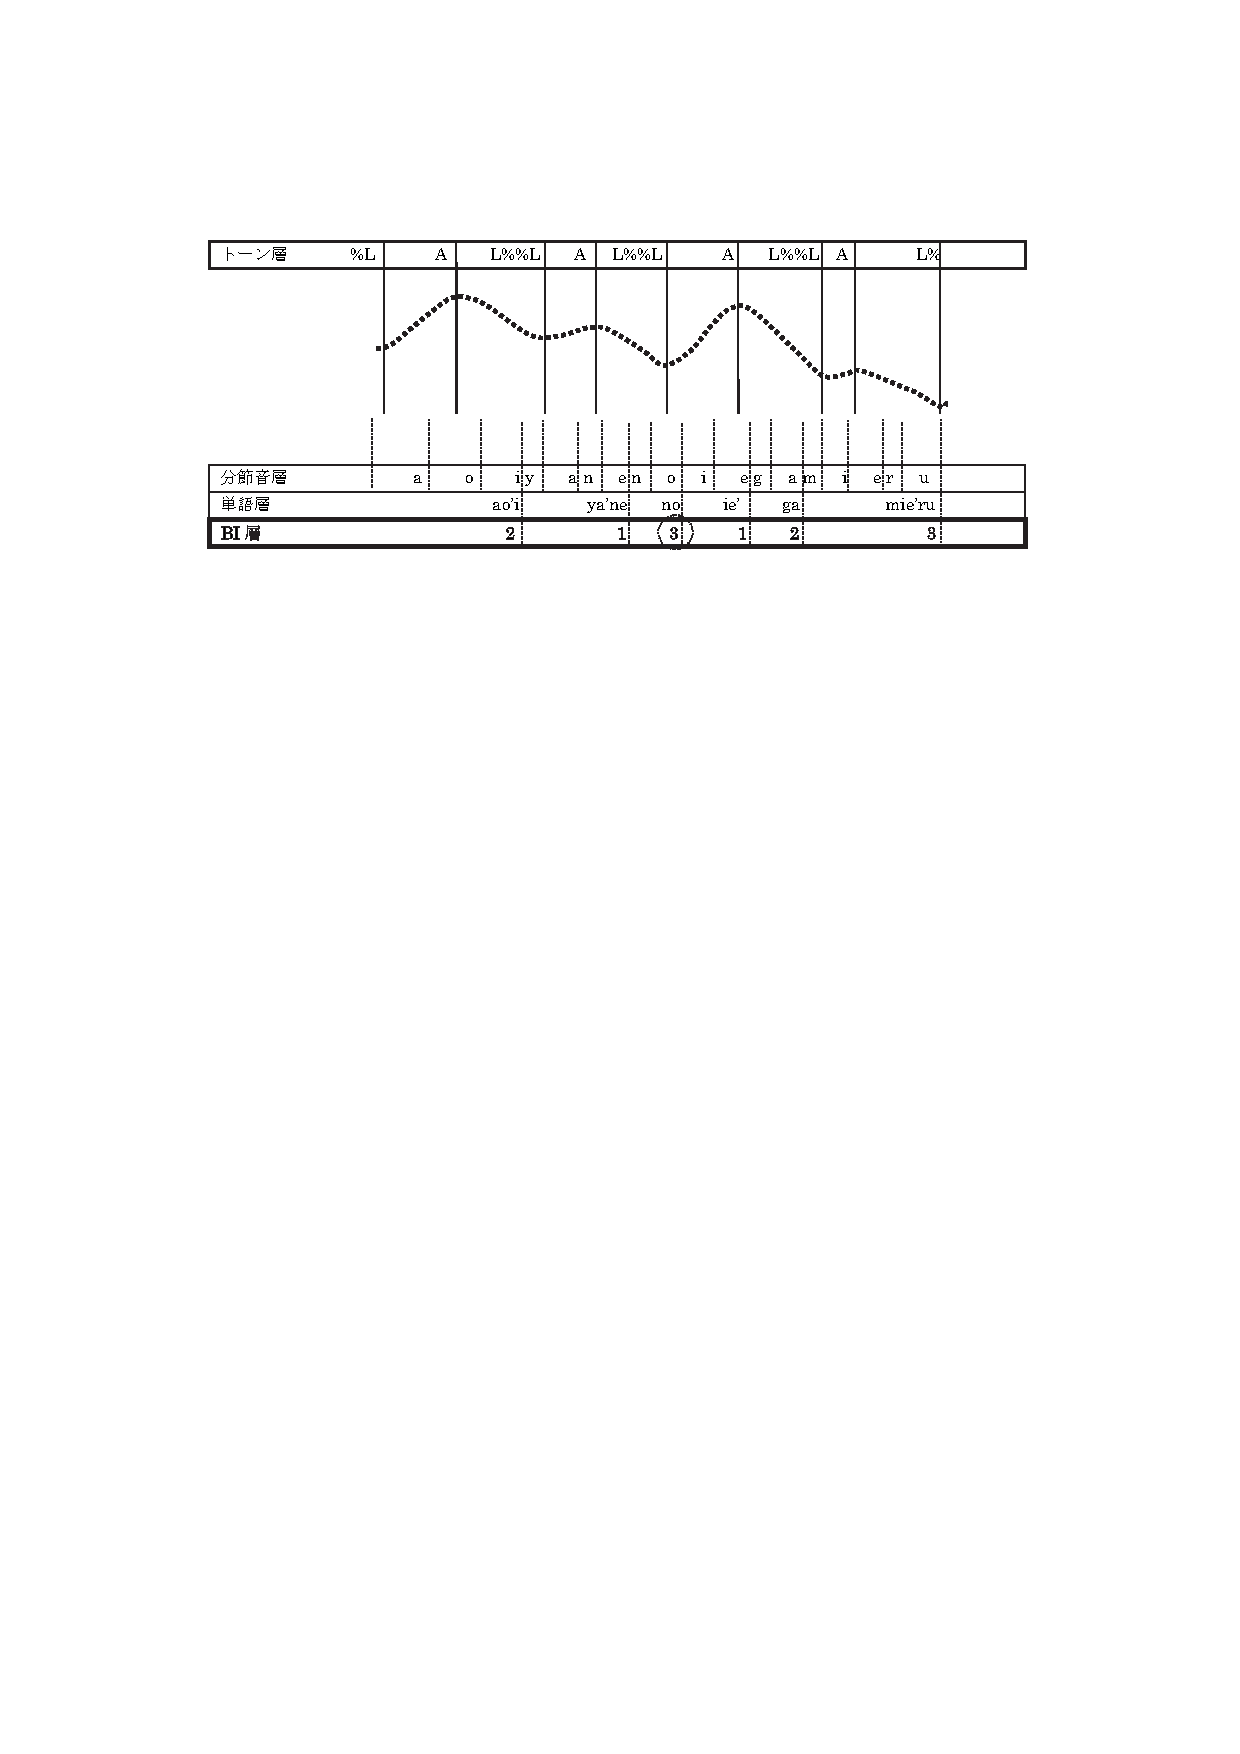
\includegraphics[width=0.7\textwidth]{figure_BIex.pdf}
 \caption{An example of annotation of BI \cite[][412]{igarashietal06}}
 \label{BIexF}
%\end{minipage}
%\end{figure}
%\begin{figure}
%\begin{minipage}{0.5\textwidth}
%\vspace{2cm}
% \centering
% 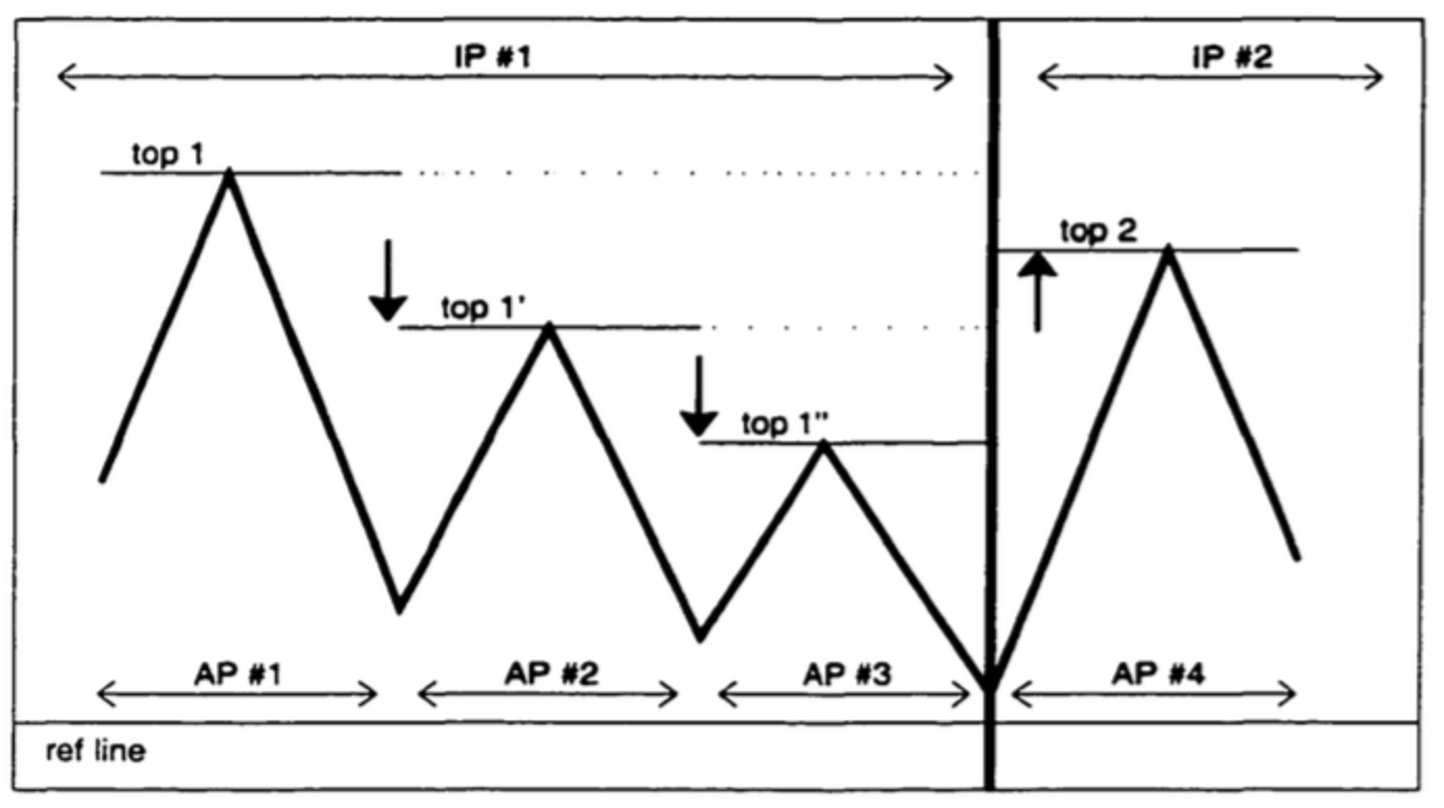
\includegraphics[width=0.5\textwidth]{figure_Venditti00_18.pdf}
% \caption{A schematic representation of down-stepping and intonational-phrase reseting in Japanese \cite[18]{venditti00}}
% \label{FigDownStep}
%\end{minipage}
\end{figure}


%An intonational phrase roughly corresponds to
%an intermediate phrase and utterance in \citeA{pierrehumbertbeckman88},
%and a major phrase and intonational phrase in \citeA{selkirktateishi91}.
%The correspondence is not one-to-one because
%some level in a theory lacks in another theory.
%For example, \citeA{selkirktateishi91} assume three levels above the major phrase (or accentual phrase) as shown in \Next,
%whereas \citeA{pierrehumbertbeckman88} assume no levels between the major phrase (their intermediate phrase) and the utterance.
%In X-JToBI, 
%Pierrehumbert-Beckman's intermediate level and utterance are further integrated into a single level of intonation phrase,
%which means that there is a single level above the accentual phrase.
%The correspondence is summarized as a table in \Next,
%where ``ST91'' indicates \citeA{selkirktateishi91} and
%``PB88'' indicates \citeA{pierrehumbertbeckman88}.%
% \footnote{
% In \citeA{selkirk09}, however, the distinction between
% major vs.~minor phrases is abandoned and only a single level, a phonological phrase, is hypothesized.
% The level of utterance is also dismissed.
% }
%%
%\ex. \EM{Levels of prosody in different theories} \\
%\begin{tabular}{llll}
%\toprule
%   & ST91 & PB88 & X-JToBI \\
%\midrule
% a. & \EM{Utterance} & Utterance & \rdelim\}{3}{1.5in}[Intonational phrase]  \\
% b. & \EM{Intonational phrase} & \rdelim\}{2}{1.5in}[Intermediate phrase] & \\
% c. & \EM{Major phrase} & & \\
% d. & {Minor phrase} & & \\
%    & {(Accentual phrase)} & & \\
% e. & Prosodic word & & \\
% f. & Foot & & \\
% g. & Syllable & & \\
% h. & Mora & & \\
%\bottomrule
%\end{tabular}
%
%What is more complicated is that
%the definition of each level varies depending on theories.
%However, major phrase, intermediate phrase, and intonational phrase basically based on the domain of downstepping.
%The present study is based on X-JToBI because
%this is the only label extensively annotated in a large spoken corpus, namely CSJ.
%However, I leave open the question of whether this label is the best or not.
%I will briefly discuss this issue in Chapter \ref{Intonation}.
%Note that, in reviewing the literature in the following section,
%different theories assume different levels of prosody and
%the definition of each level also varies.

%%----------------------------------------------------
\paragraph{Intonation unit}

Based on X-JToBI,
\citeA{denetal10} and \citeA{denetal11} propose the definition of intonation unit,
which I will employ in this study.
They call it short utterance-unit as opposed to long utterance-unit,
but I use the term ``intonation unit (IU)'' throughout
since I do not discuss long utterance-units.
An intonation-unit boundary is identified
where there is an intonational phrase (the boundary labelled as \code{3} in CSJ) discussed above,
a clause boundary,%
	\footnote{
	To be more precise, this is a long utterance-unit boundary.
	See \citeA{denetal11} for the definition of this unit.
	}
or
a pause equal to or more than 0.1 seconds.
As discussed in \citeA{enomotoetal04},
it is difficult for human annotators to agree in deciding intonation-unit boundaries based on the system proposed in \citeA{duboisetal92} and \citeA{iwasaki08}.
Den and his colleagues made it possible to identify intonation units in spontaneous speech consistently across annotators.

In the following section, however,
I review studies on various kinds of intonation units including those of \citeA{duboisetal92,maekawaetal02,iwasaki08,denetal11}.
Also, whereas prominence marking, down-stepping, and boundary pitch movements are more popular topics than intonation units,
I review those studies in relation to the current study.
See \citeA{vendittietal08} for an overview of such studies.


%%----------------------------------------------------
%\subsubsection{Prominence (pitch peak)}\label{BackSubSubSecProminence}
%
%Focus
%New \& non-adjacent Given elements \cite{venditti00}
%
%%----------------------------------------------------
%\subsubsection{Nonprominence (pitch valley)}\label{BackSubSubSecNonProminence}
%
%Adjacent given elements \cite{venditti00}
%
%%----------------------------------------------------
%\subsubsection{Down-stepping}\label{BackSubSubSecDownStep}





%%----------------------------------------------------
%\subsubsection{Pause}\label{BackSubSubSecPause}

%%% 会話分析による、日本語の話題導入の方法

%%----------------------------------------------------
\subsubsection{Intonation units and related phenomena}

In this section,
I present a review of the literature on the association between prosodic units and related characteristics of language.
Note again that
the review includes various kinds of prosodic units
based on slightly different definitions,
although they agree in many cases.

%%----------------------------------------------------
\paragraph{Prominence and downstepping}

Prominence and downstepping are crucial features in determining intonation units.
It is well known that
a focus receives prominence (pitch peak).
\citeA[99--101]{pierrehumbertbeckman88} report that
``sequences with focus on the noun almost always had an intermediate phrase [i.e., intonational phrase] boundary between the adjective and the noun[...] an intermediate phrase boundary blocks catathesis [i.e., downstepping]'',
through production experiments,
where subjects were asked to produce a sequence of an adjective and a noun with different focus positions.
Target sentences and contexts Pierrehumbert and Beckman used are like the one in \Next.
The capital letters indicate that those words are in focus, and
the bold-faced letters indicate that they are the targets of analysis.
%
%\ex.
% \a.[Q:] [In America,] are there sweet beans like there are in Japan?
% \bg.[A:] mame-wa ari-masu-ga \EM{AMAI} \EM{mame}-wa ari-mase-n \\
%      bean-\ab{top} exist-\ab{plt}-though sweet bean-\ab{top} exist-\ab{plt}-\ab{neg} \\
%      `There are beans, but there aren't SWEET beans.'
%  \b.[]    \hfill{\cite[59]{pierrehumbertbeckman88}}
%
\ex.
 \a.[Q:] [In America,] are there sweet beans or carrots like there are in Japan?
 \bg.[A:] amai {NINZIN}-wa ari-masu-ga \EM{amai} \EM{MAME}-wa ari-mase-n \\
          sweet carrot-\ab{top} exist-\ab{plt}-though sweet bean-\ab{top} exist-\ab{plt}-\ab{neg} \\
      `There are sweet CARROTS, but there aren't sweet BEANS.'
 \b.[]   \hfill{\cite[59]{pierrehumbertbeckman88}}

Pierrehumbert and Beckman showed that
there is an intonational phrase (i.e., intermediate phrase) boundary
between the adjective (\ci{amai} `sweet' in \Last[A]) and the noun (\ci{mame} `bean' in \Last[b])
when the noun is focused as in \Last.
Although the results are complicated,
they conclude that their generalization applies to both accented and unaccented words.%
 \footnote{
 \citeA{kubozono07} compared two definitions of downstepping (syntagmatic and paradigmatic) and investigated whether a pitch reset occurs before the focus.
 He found conflicting results;
 from a syntagmatic perspective, the focus receives higher pitch than the preceding phrase, which indicates that downstepping is blocked.
 From a paradigmatic perspective, on the other hand,
 he had to conclude that downstepping is not blocked before the focus.
 The present study employs the definition of syntagmatic downstepping
 and assumes that the conclusions in \citeA{pierrehumbertbeckman88} and \citeA{kubozono07} do not contradict each other.
 See \citeA{kubozono07} for detailed discussion on this issue.
 }

%%% フォーカスがピッチリセットを引き起こすか(kubozono, PB, Poser)
%%% contrastive focusと普通のフォーカスの音調の違い (郡)


%%----------------------------------------------------
\paragraph{Focus projection}

There has been a cross-linguistic question of how
human beings distinguish broad focus and narrow focus:
the issue of focus projection.
This has been investigated based on English, German and Dutch
\cite{selkirk84,gussenhoven83}.
\citeA{ito02}, who investigated this question in Japanese,
compared the response time and acceptability of each of the intonation types in \Next[A1-A3]
followed by a broad focus question like \Next[Q].
The capital letters indicate the phrases whose pitch range is expanded.
\ex.
 \ag.[Q:] yokoyama-kun-wa boonasu morat-tara doo suru-no \\
          Yokoyama-\ab{hon}-\ab{top} bonus get-\ab{cond} how do-\ab{q} \\
          `What will Mr.Yokoyama do when he gets a bonus?'
 \bg.[A1:] kare-wa \EM{DAIBINGU-o} \EM{HAZIMERU-n-da-yo} \\
           \ab{3}\ab{sg}-\ab{top} diving-\ab{acc} begin-\ab{nmlz}-\ab{cop}-\ab{fp} \\
           `He starts (scuba) diving.'
 \bg.[A2:] kare-wa \EM{DAIBINGU-o} \EM{hazimeru-n-da-yo} \\
           \ab{3}\ab{sg}-\ab{top} diving-\ab{acc} begin-\ab{nmlz}-\ab{cop}-\ab{fp} \\
           `He starts (scuba) diving.'
 \bg.[A3:] kare-wa \EM{daibingu-o} \EM{HAZIMERU-n-da-yo} \\
           \ab{3}\ab{sg}-\ab{top} diving-\ab{acc} begin-\ab{nmlz}-\ab{cop}-\ab{fp} \\
           `He starts (scuba) diving.'
% \ag. kare-wa \EM{ie-o} \EM{kariru-n-da-yo} \\
%      \ab{3}\ab{sg}-\ab{top} house-\ab{acc} rent-\ab{nmlz}-\ab{cop}-\ab{fp} \\
%      `He rents a house'
% \bg. kare-wa \EM{ie-o} {kariru-n-da-yo} \\
%      \ab{3}\ab{sg}-\ab{top} house-\ab{acc} rent-\ab{nmlz}-\ab{cop}-\ab{fp} \\
% \bg. kare-wa {ie-o} \EM{kariru-n-da-yo} \\
%      \ab{3}\ab{sg}-\ab{top} house-\ab{acc} rent-\ab{nmlz}-\ab{cop}-\ab{fp} \\
      \hfill{\cite[412]{ito02}}

Ito found that
``though dual prominence [like \Last[A1]] is preferred for answers to broad focus questions,
utterances with a single intonational prominence on the object [like \Last[A2]] may be comprehended equally quickly as those with dual prominence'' (op.cit.: 413),
whereas A1 is significantly more acceptable than A2.
Also, she reports that the response time and acceptability of the A3-type do not significantly differ from those of A1 and A2.
She concluded that
``it is possible that the relation between argument structure and intonational focus marking is not universal'' (ibid.).

%The results reported in \citeA{kori11}, on the other hand,
%suggest that the intonation of broad and narrow focus is different.
%
\citeA{kori11} investigated intonation of broad and narrow focus and
reports that, by default,
only the first word receives pitch peak and the following word is
suppressed,
although some speakers put prominence on the second word too.
\Next[a] is the target sentence that he asked participants to read aloud
and \Next[b-c] are contexts.
In \Next[b-c], both \ci{aoi} `blue' and \ci{mahuraa} `scarf' are focused
because both of them contrast with `red' and `gloves' or `sweater', respectively.
In \Next[d], \ci{aoi} `blue' is narrowly focused
because only \ci{aoi} `blue' contrasts with `red' and
`scarf' is not contrasted.
%
\ex.
 \ag. \EM{aoi} \EM{mahuraa}-dat-ta-n-desu \\
      blue scarf-\ab{cop}-\ab{past}-\ab{nmlz}-\ab{cop}.\ab{plt} \\
      `(It) was a blue scarf.'
 \b. I ordered \EMi{red gloves}, but I received \EM{a blue scarf}. \hfill{(Broad focus)}
 \b. I ordered \EMi{a red sweater}, but I received \EM{a blue scarf}.\hfill{(Broad focus)}
 \b. I ordered \EMi{a red scarf}, but I received \EM{a blue scarf}. \hfill{(Narrow focus)}

Kori concludes that
the default intonation for broad focus is to suppress the second word (\ci{mahuraa} `scarf' in this case)
because most of the participants produced the sentences as such,
although some participants chose the sentence with prominence both on \ci{aoi} `blue' and \ci{mahuraa} `scarf'
when they were asked to choose a good sentence.

%%%----------------------------------------------------
%\paragraph{Syntactic structure}
%
%\citeA{selkirk09} propose the hypothesis that
%``the clause structure of a sentence in Japanese
%corresponds to a domain for certain of the phonological and phonetic phenomena that contribute to defining the intonational patterns of Japanese sentence.
%This domain has been referred to as the $\iota$-domain, or intonational phrase'' \cite[66]{selkirk09}.
%Selkirk proposes two pieces of evidence that support her hypothesis,
%one of which is from \citeA{kawaharashinya08},
%who investigated the intonation of gapping and coordination in Japanese.
%Here I only introduce the first piece of evidence Selkirk provides
%because the second one seems to me to require further investigations.
%Kawahara and Shinya assume that
%prosodic and syntactic structures have some correspondence
%and explored the associations between them.
%Assuming that there are four levels above the phonological word,
%they hypothesized the correspondence as schematized in \Next.
%%
%\exg.
% {Syntactic boundaries:} $_{Sentence}$[... $_{Clause}$[... $_{VP}$[... {\hspace{0.2cm}} $_{NP}$[... ] ...] ...] ...] \\
% {\it Prosodic boundaries:} Utt IP MaP {\hspace{0.2cm}} MiP \\
% \hfill{\cite[65]{kawaharashinya08}}
%
%In a clause, corresponding to their intonational phrase,
%they found initial rise, pitch reset, final lowering, final pause, and final creakiness.
%In a VP, assumed to correspond to their major phrase,
%they found initial rise and pitch reset,
%both of which are smaller than those of intonational phrases,
%but found no final lowering, final pause, and final creakiness.
%
%%The second piece of evidence for the hypothesis of syntax-phonology correspondence is from \citeA{ishihara02}.
%%\exg. 
%
%%%% 統語構造の曖昧性を韻律で解決する (心理言語学の人たち)
%%%% Kawahara & Shinya (2008): 節頭のpitch riseのほうが節中のpitch riseよりも大きい → intonational phraseの存在。intonational phraseは統語構造と一致している。(Selkirk, 2009)
%%%% Deguchi & Kitagawa (2002); Ishihara (2002): 
%
%Functions of prosody to disambiguate syntactic structures are also well studied in the literature.
%For example,
%\citeA{uyenoetal80} studied how prosody affects the interpretation of syntactically ambiguous sentences like \Next,
%where \ci{ototoi} `the day before yesterday' is ambiguous over
%whether it is included in the relative clause (left-branching interpretation) or in the main clause (center-embedded interpretation).
%They manipulated the pitch peaks of relative clauses
%and had participants listen to the recording and judge whether the sentences are interpreted as left-branching or center-embedded.
%%
%\ex.
% \ag. [\EM{ototoi} koron-da otona]-ga warat-ta \\
%      day.before.yesterday fall-\ab{past} adult-\ab{nom} laugh-\ab{past} \\
%      `The adult who fell the day before yesterday laughed.'
%      \hfill{(Left-branching)}
% \bg. \EM{ototoi} [koron-da otona]-ga warat-ta \\
%      day.before.yesterday fall-\ab{past} adult-\ab{nom} laugh-\ab{past} \\
%      `The adult who fell laughed the day before yesterday.'
%      \hfill{(Center-embedded)}
% \b.[] \hfill{\cite[225]{uyenoetal80}}
%
%They found that
%``[w]hen the pitch assigned to the relative clause is the same or higher than that of the preceding portion of the sentence,
%it tends to be interpreted as center-embedded, otherwise as left-branching'' (op.cit.: 234).

%%----------------------------------------------------
\paragraph{Functional and cognitive motivations for intonation units}

\citeA{iwasaki93},
applying the style of IU identification proposed in \citeA{duboisetal92} and \citeA{chafe94}  to Japanese,
argues that a Japanese intonation unit corresponds to a phrase rather than a clause,
while \citeA{chafe87,chafe94} reports that an English IU often corresponds to a clause.
According to Iwasaki's survey,
clausal IUs in Japanese are 42.2\%,
whereas phrasal IUs are 57.8\%.
Their intonation unit is a ``stretch of speech uttered under a single coherent intonation contour'' \cite[17]{duboisetal92}.
\citeA[39]{iwasaki93} states that
the beginning of an IU ``is often, though not always, marked by a pause, hesitation noises, and/or resetting of the baseline pitch level'',
whereas the ending of an IU ``is often, again though not always, marked by a lengthening of the last syllable.''
\citeA{iwasaki93} provides \Next as an example of intonation units in Japanese corresponding to a phrase.
Each line in \Next corresponds to a single intonation unit
and \Next[a-e] as a whole consist of a single proposition
``I heard that broadcast at home with my family.''
%
\ex.
 \ag. atasi-wa-ne:* \\
      \ab{1}\ab{sg}-\ab{top}-\ab{fp} \\
      `I, you know...'
 \bg. uti-de kii-ta-no-ne? \\
      home-\ab{loc} hear-\ab{past}-\ab{nmlz}-\ab{fp} \\
      `heard at home, you know...'
 \bg. sono are-wa-ne? \\
      that that-\ab{top}-\ab{fp} \\
      `that thing, you know...'
 \bg. hoosoo-wa-ne? \\
      broadcast-\ab{top}-\ab{fp} \\
      `that broadcast, you know,'
 \bg. kazoku-de. \\
      family-with \\
      `with my family.'
 \hfill{\cite[40]{iwasaki93}}

The pitch and intensity of \Next are shown in Figure \ref{IUExF} from
\citeA[109]{iwasaki08},
where he explains the same example with the figure.
The IU \Next[a] ends with a final vowel lengthening,
whereas boundary pitch movements are observed in the ending of IUs \Next[b-d],
which are indicated by ``?''.
\Next[e] ends with a final lowering, indicated by ``.''.

Iwasaki divided the kinds of ``functional components'' into four types.
%
\ex.
 \tl{Four functional components}
 \a. \EM{Lead (LD)} such as fillers, which have no substantial meaning
 \b. \EM{Ideation (ID)}, which conveys the content of speech
 \b. \EM{Cohesion (CO)} such as conjunctives and \ci{wa}, which relates the previous and the current IUs
 \b. \EM{Interaction (IT)} such as \ci{ne} `\ab{fp}' and \ci{yo} `\ab{fp}', which is associated with communication

Based on this,
he showed the similarities among IUs.
For example, 
\Next[a] is an IU which only contains an NP followed by particles, and
\Next[b] is an IU which only contains a VP also followed by particles.
%According to the functional component classification in \Last,
The structures of these two IUs are essentially the same in terms of functional components,
although they are different in terms of grammatical structure.
%
\ex.
 \a.
  \glll [mami-ni-dake] [-wa] [-ne] \\
        Mami-\ab{dat}-only -\ab{top} -\ab{fp} \\
        \EM{ID} \EM{CO} \EM{IT} \\
 \b.
  \glll [ik-ase-ta-rasii] [-no] [-yo] \\
         go-\ab{caus}-\ab{rep} -\ab{nmlz} -\ab{fp} \\
         \EM{ID} \EM{CO} \EM{IT} \\
  \glt  `(I heard that she) let only Mami go.'
% \a.
% \glll [sooyuu sito-ga siki si] [-te] [-ne*] \\
%       such person-\ab{nom} lead do -and -\ab{fp} \\
%       \EM{ID} {} {} {} \EM{CO} \EM{IT} \\
% \glt `Such people led and...'
% \b.
% \glll [sinin-o asoko-e minnna] [-ne*] \\
%        corpse-\ab{acc} there-\ab{gl} all -\ab{fp} \\
%        \EM{ID} {} {} \EM{IT} \\
% \glt   `all the corpses to there...'
% \b.
% \glll [ano] [dote-no ue-e] [-sa*] \\
%       \ab{fl} bank-\ab{gen} top-\ab{gl} -\ab{fp} \\
%       \EM{LD} \EM{ID} {} \EM{IT} \\
% \glt  `to the top of the bank...'
% \b.
% \glll [atume] [-te.] \\
%      gather and \\
%      \EM{ID} \EM{CO} \\
% \glt `gathered and...'
% \hfill{\cite[47]{iwasaki93}}

Iwasaki analyzed his data based on his classification and
found that more than 80\% of the IUs consist of
two or less functional components.
He states that
``this might be due to the limitation of work that the speaker can handle within one IU. [...] Japanese speakers [...] are faced with a constraint which permits them to exercise up to two functions per intonation unit'' (p.~49).


\begin{figure}
 \centering
 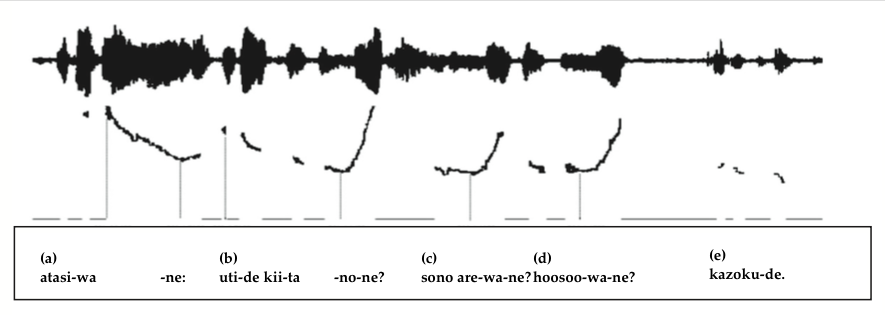
\includegraphics[width=0.85\textwidth]{sounds/iwasaki_IU.png}
 \caption{An example of an intonation unit \cite[109]{iwasaki08}}
 \label{IUExF}
\end{figure}


On the contrary, \citeA[68]{matsumoto00} reports that
``one clause comprises an average of 1.2 IUs''
and argues that
``the clause is the syntactic exponent of Japanese substantive IU''.
Instead, she proposes the ``one new NP per IU'' constraint in Japanese,
comparing it to the one new idea at a time constraint in \citeA{chafe87,chafe94}.
However, \citeA[\S 5.6]{matsumoto03} also reports that
one new or given NP per IU is preferred in Japanese conversation.
Therefore,
new as well as given NPs appear in an intonation unit
without other NPs.
%although she proposes ``one new NP per IU'' constraint
%also in this paper.


%\citeA{matsumoto03} extensively investigates the association between
%intonation units and syntactic structure, information structure, and functional structure.
%Here I review her study focusing on the association between
%intonation units and information structure.

%%%\citeA{sakutafujii}

\citeA{nakagawaetal10_piu} focused on the difference between
phrasal IUs and clausal IUs and
analyzed them in terms of information structure.
They measured referential distance and persistence \cite{givon83} and concluded that
one of the functions of phrasal IUs is to introduce or re-introduce
important topics in discourse.
They compare this function of phrasal IUs to left-dislocations observed in many languages.

%%----------------------------------------------------
%\paragraph{Other factors}
%
%length of a unit % \citeA{ghini93}
%speech rate % \citeA{hayeslahiri91}



%%----------------------------------------------------
\paragraph{Remaining issues}

Most studies on phonetics and phonology concentrate on
foci rather than topics.
Among foci, most of the studies (except for those on focus projection) concentrate on narrow focus rather than broad focus.
Moreover, almost all of them are experimental studies rather than
corpus studies.
On the other hand, I focus here on
the difference between broad foci and topics in spontaneous speech,
although I also employ a production experiment.

Functionalists such as \citeA{iwasaki93,matsumoto00,matsumoto03} and \citeA{nakagawaetal10_piu}
have methodological issues since they rely on the impressionistic definition of intonation units.
This study, on the contrary, is based on
strict definitions of intonation units and
aims at revealing associations between intonation and information structure.

The results in Chapter \ref{Intonation} show that
an intonation unit corresponds to a unit of information structure such as topic and focus,
which frequently but not always overlaps with a unit of syntactic structure.

%%----------------------------------------------------
\subsubsection{Pause}

\citeA{sugito94} showed that
pauses appear before pitch reset by means of a perceptual experiment.
She recorded trained announcers reading news and had subjects listen to the recording.
She found that, when pauses were eliminated,
subjects perceive the voice as though two people were overlapping with each other where there are pitch resets and there are supposed to be pauses.
According to her,
it is in fact impossible to reset pitch without pauses and
vocal cords are tensed 0.1 seconds before speech production.
Therefore, I assume that pauses correlate with pitch reset.

%%----------------------------------------------------
%%----------------------------------------------------
\section{Summary}

In this chapter,
I outlined the previous literature on topics and foci, and
the characteristics of Japanese related to this study,
and enumerated the remaining questions to be investigated.

In Chapters from \ref{Particles} to \ref{Intonation},
I investigate the associations between information structure and particles, word order, and intonation in spoken Japanese.
Before this,
I introduce the framework this study employs in the next chapter.





% !TEX root = ../main.tex
\chapter{Framework}\label{Framework}

%%% \isi{topic}, focusに直接対応する語順、助詞、イントネーションなどはない
%%% 下位レベルの素性で決まる
%%% Persistenceの定義
%%% CSJ-RDV版の変数名が変更されている

%%----------------------------------------------------
%%----------------------------------------------------
\section{Introduction}\label{FrameworkIntro}

In this chapter I describe the framework I employ here.
First, in \S \ref{FrameworkSemanticMap},
I introduce the theory of \isi{conceptual space} assumed throughout.
Then, I define the concepts of '\isi{topic}' and 'focus' I adopt, as well as describe the features
which have been proposed to be associated with \isi{information structure} phenomena (\S \ref{FrameworkDefinition}).
Finally,
\S \ref{FrameworkTFIdent} explains the characteristics of the corpus to be investigated and how to annotate features correlating with \isi{topic} and focus.

To investigate cognitive motivations of some linguistic category (e.g., \isi{topic} and focus),
it is possible to use a variety of clues such as generalizations about typological tendencies, models of language processing, theories of language change and language contact, language acquisition process, and language production data, as well as traditional grammaticality and acceptability judgements of sentences.
%Although it is ideal to investigate all of these clues to construct a hypothesis about human cognition of language,
This study mainly employs language production data (a.k.a.\ corpora) and
the acceptability of sentences
because these two directly reflect the intuition and cognition of adult native speakers of Japanese.
Sometimes I also use production experiments to obtain enough data
under controlled contexts.
It is necessary to investigate other kinds of clues such as typological tendencies, language processing models, and language acquisition processes of many other languages
to reveal how cognition is reflected in human language in general.
I hope that this study contributes to this larger goal.

This study restricts itself to investigating only standard Japanese,
since large spoken corpora are available in this language.
%One of the reasons for this is that
There are few empirical studies on \isi{information structure} in spoken Japanese,
while there are at least preliminary empirical studies in other languages, such as some European languages and languages in Africa \cite[e.g.,][]{cowles03,dipperetal04,dipperetal07,ritzetal08,skopeteasetal06,cookfildhauer11,chiarcosetal11}.
Another reason is that
a large spoken corpus of standard spoken Japanese is available.
% and few scholars have investigated \isi{information structure} using this corpus.
The corpus is called \ci{the Corpus of Spontaneous Japanese} (CSJ) and 
is morphologically analysed and annotated with a variety of information such as accentual phrases, intonation, parts of speech, dependent structures in addition to basic transcriptions of speech \cite{maekawa03,maekawaetal04}.
I will describe characteristics of the corpus in \S \ref{FrameworkCorpus}.


%%----------------------------------------------------
%%----------------------------------------------------
\section{Conceptual space and semantic maps}\label{FrameworkSemanticMap}

Throughout this study,
I assume a theory of \isi{conceptual space} \cite{croft01,haspelmath03}.
A \isi{conceptual space} is a multi-dimensional model of concept sensitive to some linguistic function(s).
As \citeA[93]{croft01} states,
``\isi{conceptual space} is a structured representation of functional structures and their relationships to each other. [...] Conceptual space is also multidimensional, that is, there are many different semantic, pragmatic, and discourse-functional dimensions that define any region of \isi{conceptual space}''.
It is claimed to be universal.
An example of \isi{conceptual space} is shown in Figure \ref{FrameworkCSF}.
This is a \isi{conceptual space} of parts of speech.
The horizontal dimension given in capital letters indicates
``the constructions used for the propositional acts of reference, modification, and \isi{predication}'' \cite[][p.\ 93]{croft01}.
The vertical dimension indicates the semantic classes of ``the words that fill the relevant roles in the propositional act constructions''  (op.cit.: 94).

Whereas
``the \isi{conceptual space} is the underlying conceptual structure,
[...] a \isi{semantic map} is a map of language-specific categories on the \isi{conceptual space}'' (p.\ 94).
While \isi{conceptual space} is supposed to be universal,
semantic maps are language-specific.
Figure \ref{FrameworkSMF} is an example of a \isi{semantic map} of parts of speech specific to Japanese.
The dimensions are suppressed for the purpose of convenience.
The figure shows that
nouns such as \ci{hon} `book' accompany \ci{no} to modify another noun and \ci{da} for \isi{predication}. %(58-59)
Adjectives such as \ci{yasu} `cheap' accompany \ci{i} for both modification and \isi{predication}. %(60-61)
Some nominal adjectives between `book' and `cheap' such as \ci{heewa} `peace(ful)' and \ci{kenkoo} `health(y)' accompany both \ci{no} and \ci{na} for modification and \ci{da} for \isi{predication}.
They are different from but similar to nouns such as `book'.
Some nominal adjectives such as \ci{atataka} `warm' and \ci{tiisa} `small' accompany both \ci{na} and \ci{i} for modification, and
`warm' allows both \ci{da} and \ci{i} to follow in \isi{predication}.
This indicates that
they are similar to adjectives rather than nouns.
The nominal \isi{adjective} \ci{kirei} `pretty' is in between;
it only allows \ci{na} for modification and \ci{da} for \isi{predication}.

\begin{figure}
 \fittable{
 \begin{tabular}{lclclclc}
             & \textsc{Reference} &  & \textsc{Modification} &  & \textsc{Predication} & & \\
 \textsc{Objects}     & Object    &  & Object       &  & Object      &  & Identity \\
\hhline{~~-~-~-~}
             & reference &  & modifier     &  & \isi{predication} &  & \isi{predication} \\
             & \hfill $|$ \hfill &  &  \hfill $|$ \hfill &  &  \hfill $|$ \hfill &  &  \\
 \textsc{Properties}  & Property  &  & Property     &  & Property    &  & Location \\
\hhline{~~-~-~-~}
             & reference &  & modifier     &  & \isi{predication} &  & \isi{predication} \\
             & \hfill $|$ \hfill &  &  \hfill $|$ \hfill &  &  \hfill $|$ \hfill &  &  \\
 \textsc{Actions}     & Action    &  & Action       &  & Action      &  &  \\
\hhline{~~-~-~~~}
             & reference &  & modifier     &  & \isi{predication} &  &  \\
 \end{tabular}
 }
 \caption{Conceptual space for parts of speech \cite[92]{croft01}}
 \label{FrameworkCSF}
\end{figure}

\begin{figure}
 \centering
 \begin{tabular}{clll}
                     &              & \textsc{Modification} & \textsc{Predication} \\
 \textsc{Objects}    & `book'       & \cellcolor[gray]{.8} \ci{no}         & \cellcolor[gray]{.95}  \ci{da} \\
  \vdots             & `peace(ful)' & \cellcolor[gray]{.75} \ci{no}/\ci{na} & \cellcolor[gray]{.95}  \ci{da} \\
  \vdots             & `health(y)'  & \cellcolor[gray]{.75} \ci{no}/\ci{na} & \cellcolor[gray]{.95}  \ci{da} \\
  \vdots             & `pretty'     & \cellcolor[gray]{.85} \ci{na}         & \cellcolor[gray]{.95}  \ci{da} \\
  \vdots             & `warm'       & \cellcolor[gray]{.8} \ci{na}/\ci{i}  & \cellcolor[gray]{.87} \ci{da}/\ci{i} \\
  \vdots             & `small'      & \cellcolor[gray]{.8} \ci{na}/\ci{i} & \cellcolor[gray]{.9} \ci{i} \\
 \textsc{Properties} & `cheap'      & \cellcolor[gray]{.9} \ci{i} & \cellcolor[gray]{.9} \ci{i} \\
 \end{tabular}
 \caption{The semantic map for the Japanese Nominal, Nominal Adjective, and Adjective constructions \cite[95]{croft01}}
 \label{FrameworkSMF}
\end{figure}

``The hypothesis of typological theory, including Radical Construction Grammar,
is that most grammatical domains will yield universals of the form-function mapping that can be represented as a coherent \isi{conceptual space}'' (p.\ 96), which is explicitly stated in \Next.
%
\ex. \label{SemanticMapHyp}\tl{Semantic Map Connectivity Hypothesis}: any relevant language-specific and construction-specific category should map onto a \EM{connected region} in \isi{conceptual space}. \hfill{(ibid.)}

Japanese parts of speech in Figure \ref{FrameworkSMF} support this hypothesis.
For example,
morphemes such as \ci{no} and \ci{na} map onto different but connected regions on the \isi{conceptual space}.
If the \isi{adjective} suffix \ci{i} could also attach to \ci{hon} `book', but not to \ci{kirei} `pretty', for example,
this would be a counter-example to the hypothesis.

There are also conceptual spaces for \isi{information structure},
and I aim here to describe semantic maps of \isi{information structure} in Japanese.
In terms of the theory of \isi{conceptual space},
each feature that has been proposed to correlate with \isi{information structure} (to be discussed in the next section) is considered to be a dimension of the \isi{conceptual space}.
Hence, the question I am pursuing here can be restated as follows:
what dimensions Japanese is sensitive to, and
how linguistic forms (i.e., particles, \isi{word order}, and intonation) in Japanese map onto the \isi{semantic map} of \isi{information structure} in Japanese.

In the following section,
I outline the definitions of \isi{topic} and focus I adopt and
the features correlating with \isi{topic} and focus
which are considered to be dimensions of \isi{conceptual space} for \isi{information structure}.

%%----------------------------------------------------
%%----------------------------------------------------
\section{Topic, focus, and correlating features}\label{FrameworkDefinition}

It has been pointed out that
there is a correlation between a \isi{topic} and
a referent that is activated, definite, specific, \isi{animate}, agent, and \isi{inferable},
and between a focus and
a referent that is inactivated, \isi{indefinite}, non-specific, \isi{inanimate}, and patient
\cite{givon76,keenan76,comrie79,comrie83}.
They form a prototype category;
e.g., topics are typically (i.e., frequently) but not always definite or \isi{animate}, and
foci are typically but not always \isi{indefinite} or \isi{inanimate}.
%In addition to these features,
%I propose that
%the correlation between a \isi{topic} and
%a referent that is \isi{inferable}, specific, and entity,
%and between a focus and
%a referent that is non-\isi{inferable}, non-specific, and proposition.
I propose that
the feature \fea{presupposed} is a necessary feature of \isi{topic},
while the feature \fea{asserted} is a necessary feature of focus.
On the other hand, other features correlate with \isi{topic} and focus respectively but are not necessarily topics or foci themselves.
The features correlated with \isi{topic} and focus are summarized in \Next.
\ex.\label{ISFeatures}
\begin{tabular}{lll}
	 & \isi{topic} & focus \\
	a. & presupposed & asserted \\
	b. & evoked & brand-new \\
	c. & definite & \isi{indefinite} \\
	d. & specific & non-specific \\
	e. & \isi{animate} & \isi{inanimate} \\
	f. & agent & patient \\
	g. & \isi{inferable} & non-\isi{inferable} \\
%	h. & entity & proposition \\
\end{tabular}

As will be shown in the following chapters,
\isi{topic} and focus are heterogeneous
and have complex features proposed in \ref{ISFeatures}.

In this section,
I will define each term in \Last.

%%----------------------------------------------------
\subsection{Topic}\label{FrameworkTopic}

A linguistic form is considered to represent a \isi{topic}
if it has the characteristics as in \ref{BackDefTopic} in \S \ref{BackSubsecDefTopic},
here repeated as \Next.
%
\ex.\label{FrameworkTopicDef}Topic is a \isi{discourse} element that the speaker assumes or presupposes to be shared (known or taken for granted) and uncontroversial in a given sentence both by the speaker and the \isi{hearer}.
%and that can be at issue at the time of \isi{utterance}.
%	That is, \isi{topic} is an element that is presupposed.

%While focus might also be activated,
%as discussed in \ref{FrameworkOthFeatures},
%being activated is not a definition feature of focus
%and if a linguistic form allows to represent a inactivated element as well as an activated element,
%it represents focus.
%
Since the proposition that ``the speaker assumes or presupposes to be shared both by the speaker and the \isi{hearer}'' is too long and complicated,
this statement is sometimes shortened to ``shared by the speaker and the \isi{hearer}'' to mean the same thing.
Remember that the statement is always the speaker's assumption
and hence avoids the paradox pointed out in \citeA{clarkmarshall81}.
The \isi{topic} is by definition presupposed to be shared both by the speaker and the \isi{hearer}.
By ``\isi{topic} is shared'',
I mean that topics are either evoked, \isi{inferable}, declining, or unused
in terms of the given-new taxonomy \ref{Back:Top:DefTop:GNTaxonomy} in \S \ref{BackSubsecDefTopic}.
By ``\isi{topic} is presupposed'',
I mean that the speaker assumes that the \isi{hearer} takes it for granted that the referent or the proposition being mentioned is known or accepted both by the speaker and the \isi{hearer}.
See also the discussion in \S \ref{BackSubsecDefTopic}.

Also, the notion of \ci{uncontroversial} is important;
topics cannot be questioned or argued against in a normal manner.
For instance,
\ili{English} noun phrases preceded by \ci{as for} or \ci{regarding} cannot be questioned or argued against.
Assuming that expressions like \ci{regarding} and \ci{as for} introduce \isi{topic} expressions \cite{kuno72,kuno76,gundel74},
this supports the idea that topics cannot be questioned or argued against.
In \Next, for example,
\ci{John} preceded by \ci{as for} or \ci{regarding} cannot be felicitously argued against as shown in \Next[B2,B2$^{\prime}$],
whereas \ci{a teacher}, which is considered to be focus,
can be argued against as in \Next[B2$^{\prime\prime}$].
%
\ex. \label{BackExJohn}\a.[A1:] Do you remember the guys we met at the last night's party?\label{BackExJohnA}
     Their names are Karl and John, I guess.
     Karl is doing linguistics at the grad school of our university.
     I forgot what languages he speaks.
     \b.[] [\{As for/Regarding\} John]$_{TOP}$, [he]$_{TOP}$ [is a teacher]$_{FOC}$.
     \b.[B2:] ??No, \EM{Rob} is a teacher.
     \b.[B2$^{\prime}$:] ??No, \{as for/regarding\} \EM{Rob}, he is a teacher.
     \b.[B2$^{\prime\prime}$:] No, John is \EM{an engineer}.
%%% 要確認

In other words, \isi{topic} expressions cannot be corrected by the next speaker in a normal manner.
I call this type of test the \ci{no}-test
 (see also the lie-test in \citeA[39]{erteschik-shir07}).

Careful readers might think that it is perfectly natural to produce an \isi{utterance} like \Next which is very similar to \Last[B2],
speculating that the \ci{no}-test is a flawed test.
The capital letters in \Next indicates that
those words are stressed.
%
\ex. \a.[B2:]\label{BackExRob} No, {ROB} is a teacher, not JOHN.

However, this does not mean that the test is flawed.
Note that the participants of this conversation would not be satisfied only with \Last;
John's information needs to be provided.
Therefore, a ``complete'' conversation is something like \Next.
%
\ex. \a.[A1:] [\{As for/Regarding\} John]$_{TOP}$, [he]$_{TOP}$ [is a teacher]$_{FOC}$. \hfill{(=\ref{BackExJohnA})}
     \b.[B2:] No, {ROB} is a teacher, not JOHN. \hfill{(=\ref{BackExRob})}
     \b.[A3:] Then what is John?
     \b.[B4:] I guess he is an engineer.

This suggests that
once B says \ci{no}, s/he must provide an alternative to the focus (as long as s/he knows).
I am inclined to label \ci{ROB} in \Last[B2] as focus
and think that the existence of examples like \LLast[B] does not invalidate the \ci{no}-test.

It is also unnatural to overtly receive topics as news
because overt acceptance indicates that they could be controversial.
For instance, as shown in \Next[B2],
topics cannot be repeated as news by the next speaker who has heard the \isi{utterance} \Next[A1],
whereas there is no problem to repeat the focus as news as in \Next[B2$^{\prime}$].
%
\ex.\label{aha} \a.[A1:] [\{As for/Regarding\} John]$_{TOP}$, [he]$_{TOP}$ [is a teacher]$_{FOC}$.
     \b.[B2:] ??Aha, \EM{John}.
     \b.[B2$^{\prime}$:] Aha, \EM{a teacher}.
%%% 要確認

I call this test the \ci{aha}-test.
The \ci{aha}-test is a natural consequence of the fact that
the truth value of a sentence is assessed with respect to \isi{topic} \cite{strawson64}.

Let us see specific examples of topics.
For instance,
as will be shown in Chapter \ref{Particles},
preposed zero-coded elements (elements without any overt particles) correspond to topics in Japanese
because the referent that the preposed element refers to is presupposed to be shared between the speaker and the \isi{hearer} as \ci{nezumi} `mouse' in \Next,
where {\O} indicates ``a \isi{zero particle}''.
	\ex. \label{FrameworkExMouse}Context: Y and H are roommates,
		who are bothered by a mouse running in their room
		and eating their leftovers.
		The cat they keep finally caught the mouse while H was out.
		When H is back, Y wants to let H know this news.
		\ag.[Y:] \EM{nezumi-\O} neko-ga tukamae-ta-yo \\
			nezumi-{\O} cat-\ci{ga} catch-\ab{past}-\ab{fp} \\
			`The cat caught (the) mouse.'
	
The referent `mouse' is interpreted as shared between the speaker and the \isi{hearer};
when the mouse is not shared between the speaker and the \isi{hearer} as in \Next,
the \isi{utterance} is infelicitous as shown by the contrast between \Next[Y] and \Next[Y$^{\prime}$].
	\ex. \label{TopDef}Context: Y and his cat is relaxing in the living room.
		H comes into the room.
		\a.[H:] Anything fun today?
		\bg.[Y:] ??\EM{nezumi-\O} neko-ga tukamae-ta-yo \\
			mouse-{\O} cat-\ci{ga} catch-\ab{past}-\ab{fp} \\
			Intended: `The cat caught a mouse.' \hfill{(=\LLast[Y])}
		\bg.[Y$^{\prime}$:] neko-ga \EM{nezumi-\O} tukamae-ta-yo \\
			cat-\ci{ga} mouse-{\O} catch-\ab{past}-\ab{fp} \\
			`The cat caught a mouse.'

When the mouse is not shared between the speaker (Y) and the \isi{hearer} (H),
the preposed \ci{nezumi} `mouse' is infelicitous as in \Last[Y],
while \ci{nezumi} in the pre-predicate position is felicitous as in \Last[Y$^{\prime}$].

%Moreover, the referent `mouse' is presupposed to be potentially at issue.
%If Y and H start to live separately and Y utters \LLast to H one year later for the first time they meet,
%it is infelicitous.%
% \footnote{
% In this case, however, the speaker may well assume that the \isi{hearer} has forgotten about the mouse because it is too trivial.
% Hence the speaker can treat the mouse as non-shared (new).
% In this case ``at-issue-ness'' is not necessary feature of topics.
% I leave this question for further study.
% }
%

Some readers might think that preposed zero-coded elements do not necessarily correspond to topics;
Instead, readers might suspect that they correspond to foci
because \ci{nezumi} `mouse' in \LLast is somehow ``new'' to the \isi{discourse},
or, more precisely,
it is not activated before the time of \isi{utterance} \LLast[Y].
However, as discussed below,
foci are not subject to a constraint such that their referent must be assumed to be shared by the speaker and the \isi{hearer}.
Typically, foci are \isi{indefinite} referents that are not shared as specified in \ref{ISFeatures}.
Since the preposed zero-coded elements in Japanese do not refer to \isi{indefinite} referents, as shown in \Last,
I categorize them as topics.

%%----------------------------------------------------
\subsection{Focus}\label{FrameworkFocus}

A linguistic form is considered to represent focus if it has the characteristics given in \ref{BackFocDef} in \S \ref{BackSubsecDefFocus},
repeated here as \Next for convenience.
%
\ex. Focus is a \isi{discourse} element that the speaker assumes to be news to the \isi{hearer} and possibly controversial.
S/he wants the \isi{hearer} to learn the relation of the \isi{presupposition} to the focus by his/her \isi{utterance}.
In other words, focus is an element that is asserted.
\label{FocDef}

A focused \isi{discourse} element is news in the sense that
the \isi{hearer} is assumed not to know the relationships between the element and the \isi{presupposition}.
For example,
consider the following example \Next.
\ex. \a.[Q:] Who broke the window?
	\bg.[A:] hanako-ga wat-ta-n-da-yo \\
		Hanako-\ci{ga} break-\ab{past}-\ab{nmlz}-\ab{cop}-\ab{fp} \\
		`HANAKO broke (it).'
	\b.[] Presupposition: ``x broke the window.''
	\b.[] Assertion: ``x = Hanako''

In \Last[A],
\ci{hanako} is shared in the sense that
her existence and identity are known by the speaker and the \isi{hearer}.
However,
\ci{hanako} is also news in relation to the \isi{presupposition}
``x broke the window'' at the time of \isi{utterance} \Last[Q].
The speaker of \Last[A] lets the \isi{hearer} learn the proposition that is assumed to be news: ``x = Hanako.''
\ci{Hanako} is the focus because
this is the part where the assertion is different from the \isi{presupposition}.

I also emphasize that the speaker thinks that the focus might be \EMt{controversial}.
This implies that another participant of the conversation can potentially argue against the focus statement.
%the focus is assumed to be possibly controversial by the speaker,
%while the \isi{topic} is not.
Therefore, the focus can be felicitously negated by the next speaker,
whereas the \isi{topic} cannot.
This is exemplified in \ref{BackExJohn}, repeated here as \Next.
%
\ex. \label{BackExJohn2}\a.[A:] Do you remember the guys we met at the last night's party?
     Their names are Karl and John, I guess.
     Karl is doing linguistics at the grad school of our university.
     I forgot what languages he speaks.
     \b.[] [\{As for/Regarding\} John]$_{TOP}$, [he]$_{TOP}$ [is a teacher]$_{FOC}$.
     \b.[B:] ??No, \EM{Rob} is a teacher.
     \b.[B$^{\prime}$:] ??No, \{as for/regarding\} \EM{Rob}, he is a teacher.
     \b.[B$^{\prime\prime}$:] No, John is \EM{an engineer}.
%%% 要確認

As shown in \Last,
(part of) the focus \ci{a teacher} can be negated felicitously,
whereas the \isi{topic} \ci{John} cannot be negated felicitously.
The concept of controversialness is more hearer-oriented and \isi{interactional} than the previous notions such as assertions, unpredictability, and unrecoverablity.
See also the discussion in \S \ref{BackSecFocus}.
%The definition (\ref{FocDef}) is essentially the same as the definition of focus \Next proposed in \citeA{lambrecht94}.
%\ex. The semantic component of a pragmatically structured proposition
%	whereby the assertion differs from the \isi{presupposition}.
%	\hfill{\cite[][p.\ 213]{lambrecht94}}

%%----------------------------------------------------
\subsection{Information structure in a sentence}\label{FrameworkIS}

%Predicate-focus structure
%Argument-focus structure
%Sentence-focus structure

Here I discuss types of \isi{information structure}.
Following \citeA{lambrecht94},
I distinguish three types of information structures within a sentence:
\EM{predicate-focus structure} (topic-comment structure),
\EM{sentence-focus structure}, and
\EM{argument-focus structure}.
%In addition to these three types,
%I further divide \isi{predicate-focus structure} into two types
%depending on the status of topics:
%\EM{the discontinuous topic} and \EM{the continuous topic}.

In \EM{the predicate-focus structure} or the topic-comment structure,
the predicate is the focus, as the name suggests.
The predicate may include the complement of the predicate.
This is exemplified in \Next[A] for \ili{English},
where the capital letters represent prominence in \ili{English}.
\ex. Predicate-focus structure
	\a.[Q:] (What did the children do next?)
	\b.[A:] [The children]$_{T}$ [went to SCHOOL]$_{F}$.
	\hfill{\cite[][p.\ 121]{lambrecht94}}

\Next[A] is an example of \isi{predicate-focus structure} in Japanese.
%
\ex.
 \a.[Q:] What is Hanako doing?
 \bg.[A:] [\EM{Hanako}-wa]$_{T}$ [syoosetu-o yon-deru]$_{F}$-yo \\
		Hanako-\ci{wa} novel-\ci{o} read-\ab{prog}-\ab{fp} \\
		`Hanako is reading a novel.'

%In this paper, I divide topics in predicate-focus structures into two types:
%discontinuous \isi{topic} and continuous \isi{topic}.
%They are exemplified in \Next[b] and \NNext[b] for \ili{English} \cite[][p.\ 153, interpretation of \isi{information structure} added]{givon76}.
%\ex. Predicate-focus structure with discontinuous \isi{topic}
%	\a. Once there was \EM{a wizard}.
%	He was very wise, rich, and was married to a beautiful witch.
%	They had two sons.
%	The first was tall and brooding, he spent his days in the forest hunting snails, and his mother was afraid of him.
%	The second was short and vivacious, a bit crazy but always game.
%	\b. Now [\EM{the wizard}]$_{T}$, he [lived in Africa]$_{F}$.%
%		\footnote{
%		The status of \ci{he} in this example is irrelevant for the current discussion and hence is ignored.
%		}
%
%\ex. Predicate-focus structure with continuous \isi{topic}
%	\a. Once there was \EM{a wizard}.
%	\b. [\EM{He}]$_{T}$ [lived in Africa]$_{F}$.
%
%\EM{The wizard} and \EM{he} in \LLast[b] and \Last[b] refers to \EM{a wizard} in \Next[a] and \NNext[a].
%However,
%they are intervened by other \isi{discourse} referents in \Next,
%while they are not in \NNext.
%I will call the former discontinuous \isi{topic}
%and the latter continuous \isi{topic}.
%Examples in Japanese are shown in \Next[b] for discontinuous \isi{topic} and \NNext[b] for continuous \isi{topic}.
%\ex. Predicate-focus structure with discontinuous \isi{topic}
%	\a. Taro and Hanako is in the room. Taro is sitting on the couch and playing a video game.
%	\bg. [\EM{hanako}-wa]$_{T}$ [hon(-o) yon-deru]$_{F}$-yo \\
%		Hanako-\ci{wa} book-\ci{o} read-\ab{prog}-\ab{fp} \\
%		`As for Hanako, she is reading a book.'
%
%\ex. Predicate-focus structure with continuous \isi{topic}
%	\a. Hanako is in the room, and
%	\bg. [hon(-o) yon-deru]$_{F}$-yo \\
%		book-\ci{o} read-\ab{prog}-\ab{fp} \\
%		`She is reading a book.'


In \EM{the sentence-focus structure},
the whole sentence is focused.
This is exemplified in \Next[A] for \ili{English},
where, again, the capital letters indicate stress.
\ex. Sentence-focus structure
	\a.[Q:] What happened?
	\b.[A:] [The CHILDREN went to SCHOOL]$_{F}$!
	\hfill{\cite[][p.\ 121]{lambrecht94}}

A Japanese example of sentence-focus structure is shown in \Next[A].
\ex. Sentence-focus structure
	\a.[Q:] What happened? 
	\bg.[A:] [hanako-ga syoosetu(-o) yon-deru]$_{F}$-yo \\
		Hanako-\ci{ga} novel-\ci{o} read-\ab{prog}-\ab{fp} \\
		`Hanako is reading a novel!'

In sentence-focus structure,
there is no explicit \isi{topic} and all the arguments (e.g., \ci{the children} and \ci{school} in \Last[A]) are part of the focus.
However, if one assumes stage topics \cite{erteschik-shir97,erteschik-shir07},
the distinction between the predicate-focus and the sentence-focus structures may not be clear.
%especially in languages with zero pronouns.
%In Japanese, for example,
%elements such as \ci{kyoo} `today' are coded by the so-called \isi{topic} marker \ci{wa} and appear to function in a way similar to topics as in \Next[a].
In \Next[a], for example,
\ci{kyoo} `today' might function as a \isi{topic} in the sense that
the truth value of the sentence is evaluated with respect to the specific time `today' (although, in this study, I do not examine stage topics in detail).
\ex. 
	\ag. [\EM{kyoo}-wa]$_{T?}$ [hanako-ga syoosetu(-o) yon-deru]$_{F}$-yo \\
		today-\ci{wa} Hanako-\ci{ga} novel(-\ci{o}) read-\ab{prog}-\ab{fp} \\
		`Today Hanako is reading a novel.'
		\bg. [\EM{Hanako}-wa]$_{T}$ [syoosetu-o yon-deru]$_{F}$-yo \\
		Hanako-\ci{wa} novel-\ci{o} read-\ab{prog}-\ab{fp} \\
		`Hanako is reading a novel.'

Note that, in terms of \isi{information structure},
\Last[a] is similar to \Last[b],
which has \isi{predicate-focus structure}.
The predicate-focus and sentence-focus structures are similar
in that the predicate is in the domain of focus.
For this reason, I sometimes put the predicate-focus and sentence-focus structures into the same category
and refer to them as \EM{\isi{broad focus} structures}.

In \EM{the argument-focus structure},
elements other than predicates are focused.
This is exemplified in \Next[A] for \ili{English}
and \NNext[A] for Japanese.
This structure is sometimes referred to as the \EM{\isi{narrow focus} structure}
as opposed to \isi{broad focus} structure
because the domain of focus is limited to arguments or other elements except for predicates.
\ex. Argument-focus structure
	\a.[Q:] Who went to school?
	\b.[A:] [The CHILDREN]$_{F}$ [went to school]$_{T}$. \hfill{\cite[][p.\ 121]{lambrecht94}}

\ex. Argument-focus structure
	\a.[Q:] Who is reading a book?
	\bg.[A:] [hanako-ga]$_{F}$ [syoosetu(-o) yon-deru]$_{T}$-yo \\
		Hanako-\ci{ga} book(-\ci{o}) read-\ab{prog}-\ab{fp} \\
		`Hanako is reading a book.'

%Note that sentences where only the predicate is focused are of broad-focus structure.

%Definition of information, element, entity, etc.
I distinguish between two types of components constituting an \isi{information structure}:
\isi{discourse} element and \isi{discourse} referent,
each of which is defined as in \Next:
\ex.
	\a. \EM{(Discourse) element}: {A unit of linguistic form (including zero \isi{pronoun}) that is uttered by the participants in \isi{discourse}.}
	\b. \EM{(Discourse) referent}: {An entity or proposition that a \isi{discourse} element refers to (if a referent is a proposition, it is also called \EM{proposition}).}



%%----------------------------------------------------
\subsection{Other features correlating with topic/focus}\label{FrameworkOthFeatures}

This section discusses the definition of features which have been
proposed to correlate with \isi{topic} and focus.
Although I do not necessarily annotate all the features in my corpus,
I discuss all of them
since, in some place or other, they are relevant to my proposals.

%%----------------------------------------------------
%\subsubsection{Presupposition vs. assertion}


%%----------------------------------------------------
\subsubsection{Activation cost}\label{FrameworkActivation}
The \isi{activation cost} of a referent is the assumed cost for the \isi{hearer} to activate the referent in question.
An active referent is a referent
that the speaker assumes to be in the attention of the \isi{hearer} (and hence the \isi{activation cost} is low),
while an inactive referent is a referent
that the speaker does not assume to be in the attention of the \isi{hearer} (and hence the \isi{activation cost} is high)
\cite[see also][inter alia]{chafe94}.%
	\footnote{
	I am using the term \ci{attention} rather than \ci{consciousness}
	because I believe the speaker's ability to evaluate the \isi{hearer}'s state of mind is eventually related to joint attention \cite{tomasello99}.
	}
Typically,
referents are assumed to be brought to the \isi{hearer}'s attention
by mentioning them or putting them in the \isi{hearer}'s area of visual perception.

A \isi{topic} referent is often, but not always, activated in the \isi{hearer}'s mind.
In \ref{FrameworkExMouse},
the referent `mouse' is not necessarily considered to be active in H's mind.
Although the mouse kept bothering Y and H sometimes when they were in their room,
it is not appropriate for the speaker to assume that the mouse is in H's attention anymore in school when the speaker happened to talk to H.

According to \citeA{dryer96},
focus is an element that is not activated.
While this generalization well captures the view that the focus is the stressed linguistic element,
I will not employ this definition of focus in this study
because if \ci{nezumi} `mouse' in \ref{FrameworkExMouse} is focus,
one has to come up with an explanation for why it is assumed to be shared between the speaker and the \isi{hearer},
which is typically not the case with focus.
According to my account, on the other hand,
\ci{nezumi} `mouse' in \ref{FrameworkExMouse} is \isi{topic} because the the characteristics are in accordance with \isi{topic} correlation features in \ref{ISFeatures}
and a special account for why \ci{nezumi} `mouse' is shared is not necessary.
For detailed discussion of the relationships between focus and stress,
see \citeA[Chapter 5]{lambrecht94}.

A focus referent, on the other hand, is typically assumed not to be active in the \isi{hearer}'s mind.
As \citeA{lambrecht94} has pointed out,
the most frequent focus structure is \isi{predicate-focus structure} as in \Next[A,B],
where elements included in the \isi{predicate focus} are typically not active in the \isi{hearer}'s mind.
\ex.\label{tomodati} \a.[Q:] What did you guys do today?
	\bg.[A:] [watasi-wa]$_{T}$ [tomodati-to resutoran-de supagetii tabe-ta]$_{F}$-yo \\
			\ab{1}.\ab{sg}-\ci{wa} friend-with restaurant-\ab{loc} spaghetti eat-\ab{past}-\ab{fp} \\
			`I ate spaghetti with (a) friend in (a) restaurant.'
	\bg.[B:] [boku-wa]$_{T}$ [uti-de hon yon-de-ta]$_{F}$-yo \\
			\ab{1}.\ab{sg}-\ci{wa} home-\ab{loc} book read-\ab{prog}-\ab{past}-\ab{fp} \\
			`I was reading (a) book at home.'

In \Last,
it is reasonable to assume that
Q did not have `friend', `restaurant', `spaghetti', `home', and `book' in his/her attention at the time of \isi{utterance} \Last[Q].
%I also use the term \EM{new} interchangeablly with ``inactivated.''

There is another type of \isi{activation status}: \fea{semi-active}.
I use the term \ci{declining} specifically for the referent that has been active but starts to decline because other referents are also activated.
Declining elements are in \isi{semi-active state}.

%%----------------------------------------------------
\subsubsection{Definiteness}\label{Fr:Definition:TFFeathers:Definite}

A definite referent is a referent
that is unique in the domain of \isi{discourse},
while an \isi{indefinite} referent is a referent
that is not unique in the domain of \isi{discourse}.

The claim that ``\isi{topic} is a \isi{discourse} element that the speaker assumes or presupposes to be shared (known or taken for granted) and uncontroversial in a given sentence both by the speaker and the \isi{hearer}'' in \ref{FrameworkTopicDef} 
might lead to the interpretation that the \isi{topic} is definite.
As has been pointed out in the literature \cite{givon76,keenan76,comrie79,comrie83},
topics tend to be definite.
However, this is not a necessary nor sufficient feature of topics.
Let us discuss the following example \Next.%
	\footnote{
	I am grateful to Yoshihiko Asao
	for pointing out this type of example.
	}
\ex.\label{Fr:Definition:TFFeathers:Definite:Ex:Mango1}Context:
	Y told H that he had never seen and eaten mangoes.
	H told Y that they are delicious.
	Several days later, Y finally ate a mango.
	\ag.[Y:] \EM{mangoo} konoaida miyako-zima-de tabe-ta-yo \\
			mango the.other.day Miyako-island-\ab{loc} eat-\ab{past}-\ab{fp} \\
			`(I) ate (a) mango (we talked about) in Miyako island the other day.'

In \Last `mango' is \isi{indefinite} because the mango Y ate is not unique in the domain of \isi{discourse}; H cannot uniquely identify which mango Y ate.%
 \footnote{
 \chd{Yuji Togo and one of the reviewers (Morimoto) cast doubt on my claim
      that \ci{mangoo} in \ref{Fr:Definition:TFFeathers:Definite:Ex:Mango1} is \isi{indefinite};
      Rather, they suggest that it could be generic.
      I am reluctant to accept this view because
      this \ci{mangoo} seems to refer to a specific (non-generic) mango
      that Y ate, as indicated by the past tense of the predicate \ci{tabe-ta} `eat-\ab{past}'.
%      On the other hand, I share the intuition that this preposed \ci{mangoo}
%      is not just a specific mango.
      }
 }
However, the element \ci{mangoo} `mango' is preposed because it has been discussed and hence is assumed to be shared between the speaker and the \isi{hearer}.
This makes it possible for \ci{mangoo} to appear clause-initially as will be discussed in Chapter \ref{WordOrder}.
%This is exemplified more clearly
%in the contrast between \Next[Y2] and \Next[Y2$^{\prime}$].
%\ex.\label{Fr:Definition:TFFeathers:Definite:Ex:Mango2}Context:
%	Y and H have not met for a few months.
%	\a.[H1:] What did you do these days?
%	\bg.[Y2:] ??\EM{mangoo} konoaida miyako-zima-de tabe-ta-yo \\
%			mango the.other.day Miyako-island-\ab{loc} eat-\ab{past}-\ab{fp} \\
%		\hfill(=\LLast[Y])
%	\bg.[Y2$^{\prime}$:] konoaida miyako-zima-de \EM{mangoo} tabe-ta-yo \\
%			the.other.day Miyako-island-\ab{loc} mango eat-\ab{past}-\ab{fp} \\
%			`(I) ate (a) mango in Miyako island the other day.'
%
%In \Last,
%Y and H have not discussed mango before and hence preposing \ci{mangoo} `mango' as in \Last[Y2] is infelicitous,
%while that in the pre-predicate position as in \Last[Y2$^{\prime}$] is felicitous.
%Therefore,
%a \isi{topic} is an element that is shared by the speaker and the \isi{hearer}.
%It is frequently definite, but not necessarily.
%I categorize this kind of shared indefinites into \EM{unused} borrowing the term from \citeA{prince81}.
I include this type of example in the category of unused,
extending the term ``unused'' in \citeA{prince81}.

However,
some \isi{indefinite} referents are more difficult to interpret as topics than others.
For example, expressions such as \ci{dareka} `somebody' and \ci{oozee-no hito} `many people' are poor candidates for \isi{topic} than others
judging from the fact that they cannot be followed by \ci{wa}, but can be followed by \ci{ga} in Japanese as shown in \Next \cite[][p.\ 37 ff.]{kuno73}.
As will be shown in Chapter \ref{Particles},
\ci{wa} codes the element whose referent is assumed to be active in the \isi{hearer}'s mind;
\ci{wa} codes active topics.
On the other hand, as will also be shown in Chapter \ref{Particles},
\ci{ga} codes focus elements.
\ex. \a. \EM{dareka-\{??wa/ga\}} byooki-desu \\
		somebody-\ci{wa/ga} sick-\ab{cop}.\ab{plt} \\
		`Speaking of somebody, he is sick.'
	\b. \EM{oozee-no} \EM{hito-\{??wa/ga\}} paatii-ni ki-masi-ta \\
		many-\ab{gen} person-\ci{wa/ga} party-to come-\ab{plt}-\ab{past} \\
		`Speaking of many people, they came to the party.'



A focus referent, on the other hand,
tends to be \isi{indefinite} rather than definite \cite{givon76,keenan76,comrie79,comrie83,dubois87}.
As has been mentioned above,
% in relation to example (\ref{tomodati}) in the previous section,
the most frequent focus structure is \isi{predicate-focus structure} exemplified in \ref{tomodati} and
it is reasonable to assume that Q in \ref{tomodati} cannot identify the referents included in the \isi{predicate focus} such as `friend', `restaurant', `spaghetti', and `book'.

%%%ほんと? to be modified.
%However, there is a tendency that \isi{argument focus} is definite.
%For example, \Next in infelicitous.
%\ex. \a.[X:] Alice broke the window.
%	\b.[Y:] No. A MAN broke it.
%
%\ex. \a.[X:] A woman broke the window.
%	\b.[Y:] No. A MAN broke it.

It is natural for \isi{topic} referents to be frequently realized by definite noun phrases.
The participants typically talk about the person or the thing whose identity is known by them.
Or sometimes they talk about people or something in more general terms.
This is an exceptional case known as a generic referent and requires a special account.
On the other hand, it is natural for focus referents to be frequently realized by \isi{indefinite} noun phrases
because, intuitively, an element that is not known by the \isi{hearer} in relation to a \isi{presupposition} is typically not shared between the speaker and the \isi{hearer}.
%They are independent persons and they encounter different people and things they do not share every day.


%%----------------------------------------------------
\subsubsection{Specificity}

A specific referent is fixed, namely, the speaker has one particular referent in his/her mind;
while a non-specific referent is not fixed,
i.e., the speaker does not have one particular referent in mind \cite{karttunen69diss,enc91,abbott94}.
\ili{Turkish} unambiguously codes specific and non-specific objects:
if the NP is coded by the \isi{accusative} \isi{case marker} \ci{-(y)i} (or \ci{-(y)u}),
it is interpreted as specific as in \Next[a],
while, if the NP is not overtly coded,
it is interpreted as non-specific as in \Next[b].
\ex. \ag. Ali bir piyano-yu kiralamak istiyor \\
	Ali one piano-\ab{acc} to.rent wants \\
	`Ali wants to rent a certain \isi{piano}.'
	\bg. Ali bir piyano kiralamak istiyor \\
	Ali one \isi{piano} to.rent wants \\
	`Ali wants to rent a (non-specific) \isi{piano}.'
	\hfill{\cite[][p.\ 4-5]{enc91}}

Specific referents like `\isi{piano}' in \Last[a] are fixed
in the sense that
the speaker wants to rent a particular \isi{piano} in his/her mind.
Non-specific referents like `\isi{piano}' in \Last[b] are not fixed
in the sense that
the speaker does not care which \isi{piano} s/he could rent;
any \isi{piano} works in \Last[b].

Topics are frequently but not always specific.
Consider the following example \Next,
which is slightly modified from \ref{Fr:Definition:TFFeathers:Definite:Ex:Mango1}.
%
\ex.\label{Fr:Definition:TFFeathers:Specificity:Mango}Context:
	Y told H that he had never seen and eaten mangoes.
	H told Y that they are delicious.
	Several days later, Y finally got a chance to eat a mango.
	\ag.[Y:] \EM{mangoo} raisyuu miyako-zima-de taberu-yo \\
			mango next.week Miyako-island-\ab{loc} eat-\ab{fp} \\
			`(I will) eat (a) mango (we talked about) in Miyako island next week.'

In this case, \ci{mangoo} is non-specific because speaker Y does not know which mango he will eat.
However, it is the \isi{topic} at the same time for the same reason discussed in association with \ref{Fr:Definition:TFFeathers:Definite:Ex:Mango1}.

There is a concept that is related to but distinct from non-specificity: genericity.
Generic referents do not represent an individual entity,
but do represent a concept or a category.
On the other hand, non-specific referents still represent an individual entity.
According to \citeA{kuno72},
generic referents are always available to be \isi{topic}.
In \Next,
the element \ci{kuzira} corresponds to a generic referent as the \isi{topic}.
%
\exg. \EM{kuzira}-wa honyuudoobutu-desu \\
		whale-\ci{wa} mammal-\ab{cop}.\ab{plt} \\
		`A whale is a mammal.' \hfill{\cite[][p.\ 270]{kuno72}}

When participants talk about generic referents,
the referent that is presupposed to be shared is the concept itself.
Therefore, generic referents are always shared
(unless the \isi{hearer} has never heard the expression in question).
As will be shown in Chapter \ref{Particles}, however,
\ci{wa} codes the element whose referent is assumed to be active or semi-active \isi{inferable} in the \isi{hearer}'s mind and
not all generic elements can be coded by \ci{wa}.


Foci, on the other hand, can be either specific or non-specific,
but tend to be non-specific.
In \Next[A],
the speaker may or may not have a particular book in his/her mind.
%
\ex. \a.[Q:] What are you going to do tomorrow?
	\b.[A:] [I]$_{T}$'m going to [read \EM{a book} tomorrow]$_{F}$.
%\ex.	 \a.[Q:] What did you do yesterday?
%	\b.[A:] [I]$_{T}$ [read \EM{a book} yesterday]$_{F}$.

In the example above,
the specificity of the book in question is not important.
Instead, the whole event of reading a book is more relevant to the question.
%In \Last[A], however,
%one can pragmatically infer from the past tense that
%there must be one specific book that the speaker read.



%%----------------------------------------------------
\subsubsection{Animacy}

An \isi{animate} referent is a living entity such as human beings, cats, and dogs,
while an \isi{inanimate} referent is a non-living entity such as computers, books, and love.
Snakes, bugs, plants, and flowers are somewhere in between.

Topic tends to be \isi{animate},
while focus tends to be \isi{inanimate} \cite{givon76,keenan76,comrie79,comrie83,dubois87}.
Although this study does not discuss \isi{animacy} very much,
it is relevant to some aspects of the distinction between
zero vs.\ overt particles,
as briefly mentioned in Chapter \ref{Particles}.


%%----------------------------------------------------
\subsubsection{Agentivity}

I employ the prototypes of the agent and the patient
discussed in \citeA[][inter alia]{dowty91}.
An agent is a referent
that typically has volition,
has sentience,
causes an event or change of state in another participant, or
moves.
On the other hand,
a patient is a referent
that typically undergoes a change of state,
corresponds to an incremental theme,
is causally affected by another participant, or
stationary relative to movement of another participant.

Agentivity or subjecthood is often discussed in association with \isi{topic} \cite[][inter alia]{li76}.
%Some scholars even claim that \isi{agentivity} is the definition of \isi{topic}.
%%% Reference???
However, it is inaccurate to assume that a \isi{topic} is limited to an agent
or that an agent is always the \isi{topic}.
It is important to keep in mind that
\isi{topic} correlates with agent or subject
but being an agent or subject itself is neither a necessary nor sufficient condition to be \isi{topic}.
Focus, on the other hand, correlates with patients.
In the same way as \isi{topic}, however,
it is inaccurate to assume that all foci are patients.
The relationships between \isi{topic}/focus and \isi{agentivity} are discussed in Chapter \ref{Particles},
in association with the distinction between zero vs.\ overt particles.


%%----------------------------------------------------
\subsubsection{Inferability}

%Participants talk about something they are interested in:
%it is often \fea{inferable} to some other things the participants or their interests are related to.
%The term \fea{inferable} is used in \citeA{prince81}
%to refer to a \isi{discourse} referent
%that the NP representing ``is linked, by means of another NP, or ``Anchor'', [...] to some other \isi{discourse} entity [\isi{discourse} referent in this paper's term].''

The term \fea{inferable} is borrowed from \citeA{prince81}
though many other scholars have discussed similar concepts \cite[e.g.,][]{havilandclark74,chafe94}.
A \isi{discourse} referent is \isi{inferable}
``if the speaker assumes the \isi{hearer} can infer it, via logical --  or, more commonly, plausible -- reasoning, from [\isi{discourse} referents] already [active] or from other inferables'' \cite[][p.\ 236]{prince81}.%
	\footnote{
	The terms are replaced according to this study's terminology.
	}
A referent is \isi{inferable} typically through
the part-whole or metonymic relationships between the referent and another referent that has been already active.
Inferable referents can be a \isi{topic}
by being assumed to be shared between the speaker and the \isi{hearer},
or can be focus.

%%%To be modified (消防車の例)
%As has also been pointed out in Prince (xxxx),
%some entities can be easily inferred in a given culture,
%while others are not.


%%----------------------------------------------------
%\subsubsection{Entity vs.\ event}
%
%Topic is typically an entity,
%while focus is more frequently an event.
%This is related to the observation that
%\isi{predicate-focus structure}, rather than \isi{argument-focus structure},
%is more common in the natural \isi{discourse} \cite{lambrecht94}.
%In \isi{predicate-focus structure},
%the \isi{topic} is an entity (e.g., \ci{Hanako} in \ci{Hanako read a book}),
%while the focus is an event (e.g., \ci{read a book}).
%Features such as % definite, specific, 
%\isi{animacy} and \isi{agentivity} are those of entities.
%Events cannot have these features.
%

%%----------------------------------------------------
%%----------------------------------------------------
\section{Methodology}\label{FrameworkTFIdent}

In this section,
I will discuss the methods in this study,
based on the definitions and assumptions of the \isi{topic} and the focus specified in the last section.
This study employs acceptability judgements,
production experiments, and
corpus annotation,
to be discussed in the following sections.
%In acceptability judgements, production experiments, or corpus study,
%it is necessary to identify topics and foci with clearly defined criteria for each methodology.
%While it is possible to control contexts in acceptability judgements and production experiments,
%it is relatively harder to define them in naturally occurring data.

%%----------------------------------------------------
\subsection{Topic and focus in acceptability judgements}

In acceptability judgements,
I sometimes employ the \ci{hee} test,
where the element in question is focus if it can be repeated after the expression \ci{hee} `really',
while it is not if it cannot.
See also the discussions in \S \ref{BackSubsecDefTopic}, \ref{BackSubsecDefFocus}, \ref{FrameworkTopic}, and \ref{FrameworkFocus}.
The \ci{hee}-test is exemplified in \Next.%
 \footnote{
  \chd{
  Read Jiro's \isi{utterance} in \ref{Fr:Method:Ex:Hebi} with exclamative intonation.
  Question intonation always works regardless of whether the element in question
  is \isi{topic} or focus.
  }
 }
\ex.\label{Fr:Method:Ex:Hebi} \ag.[Taro:] kinoo-sa [ore]$_{T}$ [hebi mi-ta-n-da]$_{F}$-yo \\
		yesterday-\ab{fp} \ab{1}\ab{sg} snake see-\ab{past}-\ab{nmlz}-\ab{cop}-\ab{fp} \\
	`Yesterday [I]$_{T}$ [saw a snake]$_{F}$!'
	\bg.[Jiro:] hee, \{??kinoo / ??taroo / hebi (mi-ta-n-da)\}! \\
			really yesterday / Taro / snake (see-\ab{past}-\ab{nmlz}-\ab{cop}) \\
			`Really, yesterday? / you? / (saw) a snake?'

Let us assume that in \Last[-Taro] it is presupposed that something happened to Taro yesterday.
Since something must always happen to Taro all the time,
this \isi{presupposition} is appropriate even in an out-of-the-blue context.
Therefore,
\ci{ore} `\ab{1}\ab{sg}' is interpreted as \isi{topic},
while \ci{hebi mi-ta-n-da} `snake see-\ab{past}-\ab{nmlz}-\ab{cop}' is interpreted as focus in this particular context.
Given this situation,
the \isi{hearer} of \Last[-Taro] can respond to this \isi{utterance} as in \Last[-Jiro]:
while the focus part \ci{hebi mi-ta-n-da} `snake see-\ab{past}-\ab{nmlz}-\ab{cop}' can be felicitously repeated followed by \ci{hee} `really',
the \isi{topic} part \ci{ore} `\ab{1}\ab{sg}',
which corresponds to \ci{taroo} in \Last[-Jiro], cannot be repeated felicitously.
Topics are identified negatively in this test.
The assumption of this \ci{hee} test is that
topics can never be taken as ``news'' or ``a surprise'' since they are assumed to be shared between the speaker and the \isi{hearer},
while foci are expected to be ``news'' or ``a surprise'' to the \isi{hearer}.

The expression \ci{kinoo} `yesterday' cannot be repeated either.
I assume that this is because \ci{kinoo} `yesterday' is also a part of \isi{presupposition}.
However, I am neutral as to whether or not \ci{kinoo} `yesterday' is a \isi{topic}
in the same sense that \ci{ore} `\ab{1}\ab{sg}' is a \isi{topic}.
It is a kind of stage \isi{topic} discussed in \ref{FrameworkIS}.
In this study I restrict myself to investigating elements which constitute arguments of sentences
and do not discuss much about the stage topics in detail.

In grammaticality judgements,
%If elements themselves are not clear as to whether they are topics or foci,
contexts will be provided
in order for topics to be typical topics (presupposed, definite, etc.)
and for foci to be typical foci (asserted, \isi{indefinite}, etc.).
Examples of contexts which prompt different focus structures are provided in \ref{FrameworkExPredFocus} to \ref{FrameworkExArgFocus},
where the target expression is \ci{koinu(-o) yuzut-ta} `gave a/the puppy'.
%
	\ex. \label{FrameworkExPredFocus}
	\a.[] \EM{Predicate-focus context}: Yesterday the speaker and his/her friend found an abandoned puppy on the street. The speaker brought it to his/her home. Today, the speaker tells the friend what happened to the puppy.
	\bg.[A:] sooieba [\EM{koinu}]$_{T}$ [\EM{yuzut-ta}]$_{F}$-yo \\
		by.the.way puppy give-\ab{past}-\ab{fp} \\
		`By the way, (I) gave the puppy (to somebody).'
%	\hfill{\movie{play}{koinut.wav}}

		\ex. \label{FrameworkExSentFocus}
		\a.[] \EM{Sentence-focus context}: the speaker and his/her friend are working in an animal shelter. The friend was absent yesterday and wants to know what happened yesterday.
		\bg.[A:] kinoo-wa [\EM{koinu} \EM{yuzut-ta}]$_{F}$-yo \\
		yesterday-\ci{wa} puppy give-\ab{past}-\ab{fp} \\
		`Yesterday (we) gave a puppy.'
%	\hfill{\movie{play}{koinuf.wav}}

\ex. \label{FrameworkExArgFocus}\a.[] \EM{Argument-focus context}
	\b.[Q:] What did you give to him?
	\bg.[A:] [\EM{koinu-o}]$_{F}$ [\EM{yuzut-ta}]$_{T}$-yo \\
			 puppy-\ci{o} give-\ab{past}-\ab{fp} \\
			`(I) gave the/a puppy.'

In predicate-focus contexts like \ref{FrameworkExPredFocus},
typically the referent of the \isi{discourse} element in question has already appeared in the context preceding the target expression;
in this example,
\ci{koinu} `puppy' has appeared in the context and the speaker and the \isi{hearer} share the identity of the puppy.
Therefore,
\ci{koinu} `puppy' is easily presupposed and is interpreted as \isi{topic}.
The speaker intends to tell the \isi{hearer} what happened to the puppy
because this news is not shared with the \isi{hearer}.
The readers may wonder
why I do not simply use a question like `what happened to the puppy?',
which typically prompts \isi{predicate-focus structure}.
This question, however,
strongly favours omitting the element \ci{koinu} `puppy'
because it appears in the immediate context.
This is the reason why
the context which prompts \isi{predicate-focus structure} like \ref{FrameworkExPredFocus} appears to be complicated.

In sentence-focus contexts like (\ref{FrameworkExSentFocus}),
on the other hand,
typically the referent is not shared;
in A of \ref{FrameworkExSentFocus},
\ci{koinu} `puppy' appears out-of-the-blue.
The whole \isi{utterance} is interpreted as news or focus.
In this case, A of \ref{FrameworkExSentFocus} can be easily preceded by
questions like `what happened yesterday?'.

Argument-focus contexts like \ref{FrameworkExArgFocus}
are typically \ci{what}- or \ci{who}-questions
that prompt a single argument as answer.
In \ref{FrameworkExArgFocus},
the question prompts \ci{koinu} `puppy' as answer.
`A gave (something)' is presupposed.


%%----------------------------------------------------
\subsection{Assumptions in experiments}

In production experiments,
I asked Japanese native speakers to read aloud sentences preceded by different contexts:
the context where the sentence is interpreted as different types of focus structures.
%\isi{predicate-focus structure} and where it is interpreted as sentence-focus structure.
The contexts that prompt different types of focus structures
are designed in the same way as discussed in the last section.

%%----------------------------------------------------
\subsection{Corpus annotation and analysis}\label{FrameworkCorpus}

In analyzing \isi{spontaneous speech},
it is relatively difficult to apply the definition of the \isi{topic} and the focus discussed above
because clean contexts are not available in contrast to the case with constructed examples.
For this reason,
I will provide the definitions of \isi{topic} and focus for the corpus investigation
based on the assumptions concerning \isi{topic} and focus discussed in \S \ref{FrameworkDefinition}.
%Before providing the definitions,
The basic idea is that, since it is difficult to determine
whether some \isi{discourse} referent is presupposed or not,
I will use \isi{information status} to approximate the given-new taxonomy (\S \ref{FW:Cor:TopFoc})
%and the persistence (discussed below)
of the referent
%to identify a \isi{topic} and a focus in the corpus
instead of the \fea{presupposed} vs.\ \fea{asserted} distinction.
The \isi{activation status} of the referent in question is approximated
by whether the referent has an \isi{antecedent} or not.
%The persistence of the referent is approximated by
%how many times the referent is mentioned in the following \isi{discourse} \cite{givon83}.

Firstly, I will discuss the characteristics of the corpus (\S \ref{FW:Cor:Cor})
and the procedure of annotating \isi{anaphoric} relations (\S \ref{FW:Cor:AnaRel}).
Then the annotations of relevant features will be discussed (\S \ref{FW:Cor:TopFoc}).
%Secondly, I will discuss how to identify topics and foci in the natural spoken corpus and the limitation of the identification process (\S \ref{FW:Cor:TopFoc}).
%Thirdly, the methods of annotating other features will be discussed (\S \ref{FW:Cor:OthFea}).
%Finally, the statistical methods employed in this study and their limitation will be discussed in \S \ref{FW:Cor:Stats}.

%%----------------------------------------------------
\subsubsection{Corpus}\label{FW:Cor:Cor}

This study investigates 12 core data of simulated public speaking 
from \ci{the Corpus of Spontaneous Japanese} \cite[CSJ:][]{maekawa03,maekawaetal04}.
The data list and basic information are summarized in Table \ref{CorpusInfoT}.
The data to be investigated are randomly chosen out of 107 core data of simulated public speaking.
Simulated public speaking is a type of speech
where the speakers talk about everyday topics
such as `my most delightful memory' or `if I live in a deserted island'.
I use the RDB version of CSJ \cite{koisoetal12} to search the corpus.

\begin{table}
	\begin{center}
	\caption{Corpus used in this study}
	\label{CorpusInfoT}
	\begin{tabular}{lllr}
	\toprule
	ID & Speaker gender (age) & Theme & Length (sec) \\
	\midrule
	S00F0014 & F (30-34) & Travel to Hawaii & 1269 \\
	S00F0209 & F (25-29) & Being a pianist & 619 \\
	S00M0199 & M (30-34) & Kosovo War & 580 \\
	S00M0221 & M (25-29) & Working at Sarakin & 654 \\
	S01F0038 & F (40-44) & Luck in getting jobs & 628 \\
	S01F0151 & F (30-34) & Trek in Himalayas & 765 \\
	S01M0182 & M (40-44) & Boxing & 644 \\
	S02M0198 & M (20-24) & Dog's death & 762 \\
	S02M1698 & M (65-69) & Dog's death & 649 \\
	S02F0100 & F (20-24) & Rare disease & 740 \\
	S03F0072 & F (35-39) & A year in Iran & 816 \\
	S05M1236 & M (30-34) & Memories in Mobara & 832 \\
	\bottomrule
	\end{tabular}
	\end{center}
\end{table}

The core data of CSJ has rich information of various kinds.
%\Next is the list of information that is relevant for this study.
I used the information in \Next to generate information relevant for this study.
%
\ex.
 \a. Utterance time
% \b. Morphological information
 \b. Dependency relation
 \b. Phrase \& clause boundary
 \b. Intonation

Relevant variables will be explained in each section.

%%----------------------------------------------------
\subsubsection{Annotation of anaphoric relations}\label{FW:Cor:AnaRel}

The information of \isi{anaphoric} relations is used
to identify \isi{topic} and focus.
Anaphoric relations are identified in the following way.
The basic procedures have been proposed in \citeA{iidaetal07} and \citeA{nakagawaden12}.
\ex.\label{AnnotationProcedure} 
	\a. \EM{Identification of grammatical function, \isi{discourse} elements, and zero pronoun}
	\b. \EM{Classification of \isi{discourse} elements}: Discourse elements are classified into categories based on what they refer to.
	\b. \EM{Identification of \isi{anaphoric} relations}:
		The link between the anaphor and the \isi{antecedent} is annotated.
%	\b. \EM{Annotation of \isi{topic} continuity}:
%		The information structural features of each \isi{discourse} element are computed
%		from the annotation of \isi{anaphoric} relations.


First,
I identified the grammatical function of clauses (a in \ref{AnnotationProcedure}),
namely A, S, vs.~P.
This is necessary in order to determine \isi{discourse} elements and zero pronouns to be investigated.
In Japanese,
pronouns such as \ci{watasi} `\ab{1}\ab{sg}', \ci{anata} `\ab{2}\ab{sg}', and \ci{kare} `\ab{3}\ab{sg}' are rare;
the most frequent \isi{pronoun} is the zero \isi{pronoun}.
In \Next,
for example, the speaker indicated by {\O$_{Sp}$} and `the dog' indicated by {\O$_{i}$} are zero pronouns,
assuming that they appear immediately before the predicates.%
	\
As shown in \Next[d],
two zero pronouns {\O$_{Sp}$} and {\O$_{i}$} can appear in the same clause;
still, native speakers have no trouble in understanding the \isi{utterance}.
\ex. \ag. yo-nen-kan amerika-de sigoto-o {\O$_{Sp}$} si-teru aida \\
			four-year-for America-\ab{loc} work-\ci{o} {\O$_{Sp}$} do-\ab{prog} during \\
			`While (I) was working for four years,'
	\bg. aa zutto kono inu$_{i}$-to issyoni eii {\O$_{Sp}$} sun-de \\
		\ab{fl} all.the.time this dog-with together \ab{fl} {\O$_{Sp}$} live-and \\
		`(I) lived with this dog all the time.'
	\bg. sikamo oo tabi-o {\O$_{Sp}$} suru toki-mo \\
		moreover \ab{fl} travel-\ci{o} {\O$_{Sp}$} do time-also \\
		`Moreover, also when (I) travel,'
	\bg. kuruma-ni {\O$_{Sp}$} {\O$_{i}$} nose-te \\
		car-\ab{loc} {\O$_{Sp}$} {\O$_{i}$} put-and \\
		`(I) put (the dog) in my car.'
	\bg. ee amerika-o tabi {\O$_{Sp}$} si-ta-to \\
		\ab{fl} America-\ab{acc} travel {\O$_{Sp}$} do-\ab{past}-\ab{q} \\
		`(I) traveled America.'
		\hfill{\code{(S02M1698: 182.88-195.87)}}
%四年間アメリカで仕事をしてる間
%あーずっとこの犬と一緒にえいー住んで
%しかもおー旅をする時も
%車に乗せて
%えーアメリカを旅したと
%(S02M1698: 182.88-195.87)

I identified 7697 \isi{discourse} elements (5234 NPs, 655 overt pronouns, and 1808 zero pronouns) from the corpus.

Second, I classified \isi{discourse} elements into 13 categories depending on what they refer to b in \ref{AnnotationProcedure}:
common referent, connective, speaker, \isi{hearer}, time, filler, exophora, question, quantifier, degree words, proposition, and other.
Although there are many categories,
only common referents are relevant for the purpose of this study.
Other categories were annotated for future studies.
Also, I limit my analyses to A, S, P, and Ex (to be discussed below).
Datives are also added for comparison.
This process leaves us
2301 elements (1662 NPs, 80 overt pronouns, and 559 zero pronouns).
However, I occasionally use data which include other kinds of elements
for detailed analysis.

Third,
I identified the \isi{anaphoric} relation for each \isi{discourse} element (c in \ref{AnnotationProcedure}).
A unique ID number is given for the set of \isi{discourse} elements which refer to the same entity.
In \Next, for example,
\ci{syoo-doobutu} `a small animal' in line a,
\ci{\O} in line c, e, and f refers to the small animal introduced in line a.
All of them are given the ID number 1 because they refer to the same entity.
The element \ci{syoo-doobutu} `a small animal' is called the \EM{antecedent} of the \EM{anaphor} \ci{\O} in line c.
In the same way, the element \ci{\O} in line c is the \isi{antecedent} of the \EM{anaphor} \ci{\O} in line e.
The element \ci{watasi} refers to another entity, the speaker,
and is given another ID number 2.
\ex.
		\begin{tabular}{llr}
		 & & ID \\
		\rowcolor{gray}
		a. & \sstack{\EM{syoo-doobutu}-ga koo tyokotyoko-to \\ ki-ta-n-desu-ne} & 1  \\
		\rowcolor{gray}
		 & `\EM{A small animal} came (towards us) with small steps.' & \\
		b. & de saisyo koo  & -- \\
		 & `and at first, so...' & \\
		\rowcolor{gray}
		c. & \sstack{ano sotira-no soto-no-hoo-kara \\ \EM{\O} nozoi-ta-mon-desu-kara} & 1 \\
		\rowcolor{gray}
		 & `uh \EM{it} looked at us from that direction, so' & \\
		d. & \ul{watasi}-wa saisyo & 2 \\
		 & `At first, I...' & \\
		\rowcolor{gray}
		e. & \EM{\O} risu-kana-to omot-ta-n-desu & 1 \\
		\rowcolor{gray}
		 & `(I) thoguht that \EM{it} was a squirrel.' & \\
%		f. & de & -- & -- \\
%		 & `and' & & \\
%		g. & t= sat-to koo & -- & -- \\
%		 & `quickly' & & \\
%		h. & are-to omot-te it-tara & -- & -- \\
%		 & `when I was thinking something,' & & \\
		f. & [...] sat-to \EM{\O} nige-tyai-masi-te & 1 \\
		 & `\EM{it} quickly ran away, and' & \\
		\end{tabular}
		\begin{flushright}
		(\code{S00F0014: 619.51-631.71})
		\end{flushright}


Using the \isi{anaphoric} relations and various information in the corpus,
I generated other relevant features to be discussed in the next section.

%%----------------------------------------------------
\subsubsection{Annotation of topichood and focushood}\label{FW:Cor:TopFoc}

%%----------------------------------------------------
\paragraph{Approximation to the given-new taxonomy}

The status of a referent in the given-new taxonomy is approximated by
whether the expression referring to the referent has an \isi{antecedent} or not.
An expression that has an \isi{antecedent} is called an \EM{anaphoric} element,
while an expression that does not have an \isi{antecedent} is called a \EM{non-anaphoric} element.
I use the term \isi{information status} to refer to the status of a referent being \isi{anaphoric} or non-\isi{anaphoric}.
\chd{Note that the terms \isi{anaphoric} vs.~non-\isi{anaphoric} are used in Chapter \ref{Particles}, \ref{WordOrder}, and \ref{Intonation} only to refer to corpus counts.}
The referent of an \isi{anaphoric} elements is assumed to be either evoked or declining in terms of the given-new taxonomy and active or semi-active in terms of \isi{activation status}.
On the other hand, the referent of a non-\isi{anaphoric} elements is \isi{inferable}, unused, or new in terms of the given-new taxonomy and
semi-active or inactive in terms of \isi{activation status}.
I prefer to use the terms of the given-new taxonomy over \isi{activation status} because
they are more fine-grained.
The correspondence among activation statuses, the given-new taxonomy, and corpus annotations are shown in Table \ref{ActStatusCorpus}.
The distinction between \isi{inferable}, declining, unused, and brand-new is judged manually when necessary.
By ``shared'', I mean the referent is evoked, declining, \isi{inferable}, or unused in terms of the given-new taxonomy.

\begin{table}
	\caption{Activation status, the given-new taxonomy, and corpus annotation}
	\label{ActStatusCorpus}
	\begin{center}
	\begin{tabular}{llll}
	\toprule
	Activation status & \multicolumn{2}{l}{The given-new taxonomy} & Corpus annotation \\
	\midrule
	Active & Evoked & & Anaphoric \\
	Semi-active & Declining &  & \\
	\rowcolor{gray}
	Semi-active & Inferable &  & \\
	\rowcolor{gray}
	Inactive & Unused & \rdelim\}{-4}{20pt}[Shared] & Non-\isi{anaphoric} \\
	\rowcolor{gray}
	Inactive & Brand-new & &  \\
	\bottomrule
	\end{tabular}\\
	\end{center}
\end{table}


%%----------------------------------------------------
\paragraph{Grammatical function}

Following \citeA{comrie78} and \citeA{dixon79},
I distinguish S, A, and P in grammatical function.
S is the only argument of \isi{intransitive} clause,
A is the \isi{agent-like argument} of \isi{transitive clause},
and P is the patient-like argument of \isi{transitive clause}.
For now, I simply distinguish A and P based on whether the argument in question is or can be coded by \ci{ga} or \ci{o}.
When it can be coded by \ci{ga}, it is A;
when it can be coded by \ci{o}, it is P.
Furthermore, I sometimes distinguish agent S and patient S if needed.
%since the distinction plays an important role in the spoken Japanese grammar.
%For now, I had to rely on the intuition to distinguish agent and patient S.
%I employ the criteria proposed in the literature to avoid unreliability.
%The criteria will be explained in the relevant chapters.

In addition to S, A, and P,
I identify non-argument elements (Ex).\label{FW:Cor:TopFoc:ExDef}
Non-argument elements are those which appear to be part of the clause but do not have direct relationships with the predicate.
A typical example is shown in \Next.
%
\exg. \EM{zoo-wa} hana-ga nagai \\
		elephant-\ci{wa} nose-\ci{ga} long \\
		`The elephant, the nose is long (The elephant has a long nose).' \hfill{\cite{mikami60}}

As exemplified in \Last,
the element \ci{zoo} `elephant' is considered to be Ex.
\ci{Hana} `nose' is the only argument of the predicate (S),
and \ci{zoo} `elephant' does not have direct relationships with the predicate \ci{nagai} `long';
still, \ci{zoo} `elephant' looks like part of the clause and needs a label,
which happens to be ``Ex''.

Although Ex is frequently coded by so-called \isi{topic} markers
such as \ci{wa} and \ci{toiuno-wa},
\ci{wa}- and \ci{toiuno-wa}-coded elements are not always labelled as Ex.
If they are considered to be S, A, or P,
they are labelled as such.
For example, in the case where \ci{hana} `nose' is coded by \ci{wa} like \Next,
\ci{nose} is labelled as S, instead of Ex.
%
\exg. zoo-no hana-wa nagai \\
      elephant-\ab{gen} nose-\ci{wa} long \\
      `The elephant's nose is long.'






%In \Last,
%the element coded by \ci{wa}, \ci{toiuno-wa}, or \ci{mo}
%are often non-arguments,
%and hence this feature needs to be annotated.


%%----------------------------------------------------
\paragraph{Other features}

Ideally, it is necessary to annotate all the variables proposed in \ref{ISFeatures},
but it is impossible to annotate all of them,
partially because of the limitation of time and labor and 
partially because of the lack of clear criteria to annotate them consistently.
For example, \isi{definiteness} and specificity are difficult to annotate consistently.
Multiple annotators are needed for reliable and objective analyses.
Animacy could be simpler, but I have not annotated this feature throughout the corpus due to the limitation of time and labor.
The previous literature indicates that
these features play little role in Japanese grammar.
These features will be discussed when necessary.

%In investigating a spoken corpus,
%\isi{topic} and focus are identified by the \isi{activation status}.
% and the persistence.
%As discussed in \S \ref{FrameworkActivation},
%activated referents are more likely to be topics.
%On the other hand, inactivated referents are more likely to be focus.
%As \citeA{lambrecht94} and many others have pointed out,
%activated referents are more acceptable topics than inactivated referents.
%The \isi{topic} acceptability scale is summarized as in \Next,
%where I paraphrased Lambrecht's terms with this study's terminology in parentheses.
%\ex. \label{TopicAcceptabilityScale}The \isi{topic} acceptability scale
%	\a.[$\uparrow$] \tl{most acceptable topic}
%	\b. active (activated)
%	\b. accessible (semi-activated/\isi{inferable})
%	\b. unused (inactivated and definite or generic)
%	\b. brand-new anchored (inactivated and maybe definite or \isi{indefinite})
%	\b. brand-new unanchored (inactivated and \isi{indefinite})
%	\b.[$\downarrow$] \tl{least acceptable topic}
%		\hfill{\cite[][p.\ 165]{lambrecht94}}
%
%Table \ref{ActStatus} is a summary of \Last and my argument so far:
%activated referents are typical, or most frequent, topics, and
%new (inactivated) referents are typical foci.
%I will keep the term ``unused'' in \Last for convenience and, henceforth,
%I will exclude unused referents from inactivated referents.
%
%\begin{table}
%	\caption{Activation status and topic/focus}
%	\label{ActStatus}
%	\begin{center}
%	\begin{tabular}{lcc}
%	\toprule
%	& Topic & Focus \\
%	\midrule
%	Activated & \cellcolor{gray}{Typical topic} & \\
%	Inferable &  & \\
%	Semi-activated &  & \\
%	Unused & & \\
%	Inactivated &  & \cellcolor{gray}{Typical focus} \\
%	\bottomrule
%	\end{tabular}\\
%	\end{center}
%\end{table}
%
%In my corpus investigation,
%the \isi{activation status} of a referent is approximated by
%whether the element referring to the referent in question has an \isi{antecedent} or not.
%I will call this approximation \EM{information status}.
%If the element has an \isi{antecedent},
%it indicates that the referent is activated
%because it has already been mentioned by the \isi{antecedent}.
%If an element has no \isi{antecedent},
%it is more likely to be inactivated in the hear's mind.
%This method is employed in annotations of \isi{information structure}
%\cite{givon83,calhounetal05,gotzeetal07}
%.
%Note, however, that
%the referent of an element without an \isi{antecedent} are not always inactivated.
%The referent may be activated through the visual perception,
%or it may be partially activated through the part-whole relations.
%To keep in mind that the correlation between the actual \isi{activation status} and having an \isi{antecedent} is not perfect,
%I will refer to the referent of an element that has \isi{antecedent} as \EM{given} referent,
%and the referent of an element without an \isi{antecedent} as \EM{new} referent.
%The relation between the \isi{activation status} and given vs.\ new distinction is summarized in Table \ref{ActStatusCorpus}.
%I assume that given referents are more likely to be topics and new referents are more likely to be foci in the corpus investigation.
%The referents that are \isi{inferable}, semi-activated, or unused will be analyzed qualitatively followed by quantitative investigations.
%
%\begin{table}
%	\caption{Activation status in the corpus}
%	\label{ActStatusCorpus}
%	\begin{center}
%	\begin{tabular}{lcc}
%	\toprule
%	& Topic & Focus \\
%	\midrule
%	Activated & \multicolumn{2}{c}{Given in the corpus} \\
%	\rowcolor{gray}
%	Inferable &  & \\
%	\rowcolor{gray}
%	Semi-activated &  & \\
%	\rowcolor{gray}
%	Unused & \multicolumn{2}{c}{New in the corpus} \\
%	\rowcolor{gray}
%	Inactivated &  & \\
%	\bottomrule
%	\end{tabular}\\
%	\end{center}
%\end{table}
%
%I will employ another diagnostics of topics and foci:
%persistence \cite{givon83}.
%A persistent referent is a referent that is mentioned more than once throughout the \isi{discourse},
%while a non-persistent referent is a referent that is mentioned only once throughout the \isi{discourse}.
%Note that I modified the criteria of persistence from Giv\'on's original ones.
%The domain where the criteria can be applied is each speech that the speaker gave, which is simply separated by files.
%I assume that persistent referents are more likely to be topics,
%while non-persistent referents are more likely to be foci
%following \cite{givon83}.

%Table \ref{TFhierarchyT}

%\begin{table}
%	\begin{center}
%	\caption{Activation status and other features of non-generic referent}
%	\label{ISFeaturesST}
%%	\small
%	\begin{tabular}{lccccc}
%	\toprule
%	& Activated & \sstack{Can be \isi{topic} \\ (or presupposed)} & \sstack{Can be Focus \\ (or asserted)} & definite & Specific \\
%	\midrule
%	\EM{Activated} & \Circle & \Circle & \Circle & \Circle & \Circle \\
%	\EM{Semi-activated} & \RIGHTcircle & \Circle & \Circle & \Circle & \Circle \\
%	\EM{Inferable} & \RIGHTcircle & \Circle & \Circle & \RIGHTcircle & \RIGHTcircle \\
%	\EM{Unused} & \CIRCLE & \Circle & \Circle & \Circle & \Circle \\
%%	\EM{Unmentioned} & \CIRCLE & \Circle & \Circle & \RIGHTcircle & \CIRCLE \\
%	\EM{Brand new} & \CIRCLE & \CIRCLE & \Circle & \CIRCLE & \RIGHTcircle \\
%	\bottomrule
%	\end{tabular}\\
%%	\hfill{(features in higher position override those in lower position)}
%	\end{center}
%\end{table}
%
%\begin{table}
%	\begin{center}
%	\caption{Activation status and other features of generic referent}
%	\label{ISFeaturesGT}
%%	\small
%	\begin{tabular}{lccccc}
%	\toprule
%	& Activated & \sstack{Can be \isi{topic} \\ (or presupposed)} & \sstack{Can be Focus \\ (or asserted)} & definite & Specific \\
%	\midrule
%	\EM{Activated} & \Circle & \Circle & \Circle & \RIGHTcircle & \CIRCLE \\
%	\EM{Semi-activated} & \RIGHTcircle & \Circle & \Circle & \RIGHTcircle & \RIGHTcircle \\
%	\EM{Inferable} & \RIGHTcircle & \Circle & \Circle & \RIGHTcircle & \RIGHTcircle \\
%%	\EM{Unused} & \CIRCLE & \Circle & \Circle & \Circle & \Circle \\
%	\EM{Unmentioned} & \CIRCLE & \Circle & \Circle & \CIRCLE & \CIRCLE \\
%%	\EM{Brand new} & \CIRCLE & \CIRCLE & \Circle & \CIRCLE & \RIGHTcircle \\
%	\bottomrule
%	\end{tabular}\\
%%	\hfill{(features in higher position override those in lower position)}
%	\end{center}
%\end{table}


%Information structure features \\ \cite[see also]{prince81,chafe94}
%\begin{table}
%	\begin{center}
%	\caption{Topic-focus distinction and given-new hyerarchy}
%	\label{TFhierarchyT}
%%	\small
%	\begin{tabular}{lcc}
%	\toprule
%	& Topic & Focus \\
%	\midrule
%	\EM{Activated} & \Circle & \Circle \\
%	\EM{Semi-activated} & \Circle &  \Circle \\
%	\EM{Inferable} & \Circle &  \Circle  \\
%	\EM{Unused} & \Circle & \Circle \\
%%	\EM{Unmentioned} & \Circle & \Circle \\
%	\EM{Brand new} & \CIRCLE & \Circle \\
%	\bottomrule
%	\end{tabular}\\
%%	\hfill{(features in higher position override those in lower position)}
%	\end{center}
%\end{table}

%%----------------------------------------------------
%\subsubsection{Annotation of other features}\label{FW:Cor:OthFea}




%%%----------------------------------------------------
%\subsubsection{Notes on statistics}\label{FW:Cor:Stats}
%
%Ideally, all the features relating to \isi{information structure} should be annotated, and
%a regression analysis should be applied to investigate
%which feature contributes to which part of spoken Japanese grammar.
%However, it turned out that
%my data is still too small to apply a regression analysis;
%%therefore, I mainly employ Fischer's exact test.
%I sometimes apply statistical tests when appropriate.
%The tool used for statistical analyses and graphics throughout the study
%is R.%
%	\footnote{
%	\href{http://www.r-project.org/}{http://www.r-project.org/}
%	}


%%----------------------------------------------------
\section{Summary}

In this chapter,
I discussed
the framework employed in this study and
the method of corpus annotation and analysis.
In the next three chapters,
different aspects of spoken Japanese grammar (i.e., particles, \isi{word order}, and intonation) will be analyzed based on the framework and methodology discussed in this chapter.









% !TEX root = ../main.tex
\chapter{Particles}\label{Particles}

%%% すべての旧情報にトピックマーカーがつくわけではない
%%% トイウノハは長い
%%% トイウノハはほとんどSにつく
%%% 文頭に出るとヲがつく
%%% grammatical functionに言及:トピックはSが多い→属性叙述
%%% African American English, Mandarinなどでコピュラがトピックマーカーになっている (Lee, 2002: Contrastive Topic)
%%% ヲがつくとdefiniteに解釈されやすいかも
%%% 話題の無助詞は新規トピックの導入 \cite{niwa06} を引用
%%% ハ vs. 話題の無助詞は活性化されているか否かの違い \cite{kaneda08} を引用
%%% トピックマーカーあり vs. なしで統計に賭ける
%%% Kuno (1972) ハの意味はanaphoric, generic, contrastive -> 統一的に説明できる
%%% ``Wa marks either the theme or the contrasted element of the sentence. The theme must be either anaphoric or generic, while there is no such constraint for the contrasted element.'' (Kuno, 1972: p.296) (Kuno 1969; 1970も参照)
%%% Contrastive wa にもちゃんと制約はある。Activateされた集合の中から選ばなければならない。
%%% ハがactivated referentsを標示する = Kuno (1973: p.40) のanaphoricとほぼ同じ
%%% 誰がパーティーに来たの? -- ジョンは来た に対する反論
%%% 誰が大金持ちですか? -- ビル・ゲイツは大金持ちです(Kuroda, 2005: p.7)
%%% cf. 誰がこの委員会のメンバーですか? -- ジョン{が/?は}メンバーです (作例)

%%% Clancy & Downing のハはcohesive divideだという議論に言及

%%----------------------------------------------------
%%----------------------------------------------------
\section{Introduction}\label{ParIntro}

In this section, I will describe
so-called topic particles coding different kinds of topics (\S \ref{TopPar})
and
so-called case particles coding different kinds of foci and grammatical functions (\S \ref{CasePar}).
Table \ref{ParInfoStatusT} summarises kinds of so-called topic particles and case particles
coding topics and focus in different statuses of given-new taxonomy.
The activation status is also specified in the table to show the correspondence,
although I mainly use the terms of given-new taxonomy.
Different topic particles attach to elements in different statuses of given-new taxonomy,
while case particles are not sensitive to the given-new taxonomy.
Instead, case particles are sensitive to the grammatical functions and the broad vs.\ narrow focus distinction,
which is summarized in Table \ref{OvertZeroCaseParT1}.
The morpheme \ab{cop} indicates copula.

\begin{table}[hbt]
	\caption{Topic particle vs.\ activation status and given-new taxonomy}
	\label{ParInfoStatusT}
	\begin{center}
	\begin{tabular}{|l|l|c|c|}
	\hhline{----}
	Activation status & Given-new taxonomy & Topic & Focus \\
	\hhline{|-|-|-|-|}
	 Active & Evoked & \ci{toiuno-wa, wa}, {\O} &  \\
	\hhline{|-|-|-|~|}
	\cellcolor[gray]{.9}Semi-active & \cellcolor[gray]{.9}Inferable & \ci{wa}, {\O} &  \\
	\hhline{|-|-|-|~|}
	 Semi-active & Declining & \multirow{2}{*}{\ab{cop}-\ci{kedo/ga}, {\O}}  & case particles, {\O} \\
	\hhline{|-|-|~|~|}
	\cellcolor[gray]{.9}Inactive & \cellcolor[gray]{.9}Unused &  &  \\
	\hhline{|-|-|-|~|}
	\cellcolor[gray]{.9}Inactive & \cellcolor[gray]{.9}Brand-new &  --  &  \\
	\hhline{----}
	\end{tabular}\\
	\end{center}
\end{table}

%\begin{table}[hbnt]
%\begin{center}
%	\caption{Topic particle vs.\ contrastiveness}
%	\label{TopicContrast}
%\begin{tabular}{lcccc}
%	\toprule
%	 & A & \multicolumn{2}{c}{S} & P \\
%\cline{3-4}
%			 & & agent & patient & \\
%	\midrule
%%	inactive Topic & \cellcolor[gray]{.9} {\O} & \cellcolor[gray]{.9} {\O}  & \cellcolor[gray]{.9} {\O} & \cellcolor[gray]{.9} {\O} \\
%%	\rowcolor{gray}
%%	Activated Topic (KJ) & {\O} & {\O}  & {\O} & {\O} \\
%	Activated Topic & \cellcolor[gray]{.9} {\O}, \ci{wa} & \cellcolor[gray]{.9} {\O}, \ci{wa} & \cellcolor[gray]{.9} {\O}, \ci{wa} & \cellcolor[gray]{.9} {\O}, \ci{wa} \\
%%	\rowcolor{gray}
%%	Contrastive Topic (KJ)  & {\O}, \ci{wa}  & {\O}, \ci{wa} & \ci{wa} & \ci{wa} \\
%	Contrastive Topic & \ci{wa} & \ci{wa} & \ci{wa} & \ci{wa} \\
%	\bottomrule
%\end{tabular}
%\end{center}
%\end{table}

\begin{table}[hbt]
	\begin{center}
	\caption{Case particle vs.\ grammatical function}
	\label{OvertZeroCaseParT1}
	\begin{tabular}{lcccc}
		\toprule
		 & A & \multicolumn{2}{c}{S} & P \\
	\cline{3-4}
				 & & Agent & Patient & \\
		\midrule
		Non-Contrastive Focus  & \ci{ga} & \ci{ga} & \ci{ga}, {\O} &  {\O} \\
		Contrastive Focus   & & & & \\
		or Formal Speech  & \ci{ga} & \ci{ga} & \ci{ga} & \ci{o} \\
		\bottomrule
	\end{tabular}
	\end{center}
\end{table}

I argue that these tables are a kind of semantic map \cite{croft01,haspelmath03}.
By arguing that Table \ref{ParInfoStatusT} and \ref{OvertZeroCaseParT1} are examples of semantic maps,
I postulate that
the scales of given-new taxonomy (the column) and the topic vs.\ focus distinction (the row) in Table \ref{ParInfoStatusT} and
the contrast vs.\ non-contrast distinction (the column) and the grammatical function (the row) in \ref{OvertZeroCaseParT1} are cognitively real and continuous in the way they are ordered in the tables.
This argument and the Semantic Map Connectivity Hypothesis \ref{SemanticMapHyp} in \S \ref{FrameworkSemanticMap} lead us to our hypotheses \Next.
%
\ex. \label{SemanticMapHypIS}
 \EM{Semantic Map Connectivity Hypothesis of Information Structure}:
 Since the scales of given-new taxonomy and the topic vs.\ focus distinction in Table \ref{ParInfoStatusT} and
the contrast vs.\ non-contrast distinction and the grammatical function in \ref{OvertZeroCaseParT1} are cognitively continuous,
	the particles
	%such as \ci{toiuno-wa}, \ci{wa}, and \ci{ga}
	map onto a connected region in the conceptual space.

The semantic maps in Table \ref{ParInfoStatusT} and \ref{OvertZeroCaseParT1}
support the hypothesis \Last because
all of the particles are in connected regions.
In the following sections,
I will show the details of the distributions of these particles
with specific examples.


%%----------------------------------------------------
%%----------------------------------------------------
\section{So-called topic particles}\label{TopPar}

As shown in Table \ref{ParInfoStatusT},
evoked elements are coded by \ci{Toiuno-wa} or \ci{wa},
while inferable elements are coded by \ci{wa}.
Declining and unused elements are coded by a copula followed by \ci{kedo} `though' or \ci{ga} `though'.
The zero particle (indicated by {\O}) can code elements in the given-new taxonomy.
%The distinction of activation statuses turned out to be insufficient to capture the different usages of topic particles in Japanese.
%I employ the given-new taxonomy (\ref{Back:Top:DefTop:GNTaxonomy}) for fine-grained analysis of activation status.
The statuses in the given-new taxonomy have corresponding activation statuses in the hearer's mind assumed by the speaker.
I propose that inferable and declining elements and unused and brand-new elements are in different activation statuses in the assumed hearer's mind.

Table \ref{ParInfoStatusCTT} and Figure \ref{ParInfoStatusCTF} show the distributions of elements in different information status coded by different particles in our corpus.
%Table \ref{ParInfoStatusT} and Figure \ref{ParInfoStatusF} show the distributions of elements coded by case particles,
%which are also put here for comparison.
Overall, the topic particles \ci{toiuno-wa} and \ci{wa} codes more ratio of anaphoric elements than the case particles \ci{ga} and \ci{o}.
The particles \ci{mo} and \ci{ni} are included here for comparison.
In the corpus, the markers \ci{wa}, \ci{toiuno-wa}, and \ci{mo} are the most frequent topic markers and 
\ci{ga}, \ci{o}, and \ci{ni} are the most frequent case markers (except for \ci{no} `\ab{gen}').
% codes new elements most frequently among the three.
%As discussed below,
%\ci{mo} can actually code focus elements and it is not a topic marker in terms of the present study's definition.
Note that ``anaphoric'' in the present work just means ``the element in question has the co-referential antecedent'' and ``non-anaphoric'' means ``it does not.''
Elements with bridging antecedents are included in ``non-anaphoric.''
See \S \ref{FW:Cor:AnaRel} for the detail of the procedure of annotation.
\chd{A linear mixed effects model was employed to predict information status.%
 \footnote{
 I used R for the statistical analysis of the thesis.
 \code{https://www.r-project.org}
 The packages \code{lme4} and \code{lsmeans} were employed.
 }
I included particles (\ci{toiuno-wa, wa, mo, ga, o, ni}), word order (\code{nth} in CSJ, see \S \ref{WO:Intro} for the definition of this annotation), and intonation (phrasal vs.~clausal IU, see \S \ref{Int:PIUCIU} for the definitions)
as fixed effects, and speakers (\code{TalkID}) as a random effect.
The model with the effects of particles, word order, and intonation is significantly different from the model without each of those effects (likelihood ratio test, $p<0.001$ a model without particles, $p<0.01$ that without word order, and $p<0.05$ without intonation).%
 \footnote{The effects of word order and intonation are to be discussed
           in Chapter \ref{WordOrder} and \ref{Intonation}, respectively.}
The least-squares mean for each level of the particles was calculated, and the pairwise comparisons among particles were conducted.
The results of this pairwise comparison is shown in Table \ref{Par:InfoStatusPar:LSMEANST},
which only includes the pairs of interest and those whose p-values are less than $0.5$.%
\footnote{
The p-values are adjusted using Tukey method for comparing a family of multiple estimates.
}
The contrast of \code{ga - o}, whose estimate is $-0.465$, indicates that
the least-squares mean of the odds ratio of anaphoric elements coded by \ci{ga} is significantly less than the least-squares mean of the odds ratio of those coded by \ci{o};
in other words, anaphoric elements are more likely to be coded by \ci{o} than by \ci{ga}.
Similarly, anaphoric elements are more likely to be coded by \ci{wa} than by \ci{ga}, by \ci{ni}, and by \ci{mo}.
The difference between the particles \ci{o} and \ci{wa}/\ci{toiuno-wa} is not statistically significant.
As will be discussed in \ref{Par:ArgStr:TopHierarchy},
this is because \ci{wa} (and presumably \ci{toiuno-wa}) prefers to code anaphoric As over anaphoric Ps.
Also, the difference between \ci{toiuno-wa} and \ci{ga} is not statistically significant
because of the effect of intonation;
most of the \ci{toiuno-wa} coded elements are in phrasal IUs (see Chapter \ref{Intonation}).
}

The statistical analysis shows that
\ci{toiuno-wa} codes as much ratio of anaphoric elements as \ci{wa} does.
However, detailed qualitative analysis in \S \ref{Toiunowa} reveals that
in fact the referents of \ci{toiuno-wa}-coded elements are evoked;
the referent of non-anaphoric elements coded by \ci{toiuno-wa} has been introduced implicitly in the previous contexts.
%Note that
%the activation status of non-anaphoric elements in the corpus can be
%inferable, unused, or brand-new
%as indicated by the gray rows of Table \ref{ParInfoStatusT}.
On the other hand,
the referent of \ci{wa}-coded elements have not necessarily been introduced in the previous contexts;
they can be inferable elements.
The zero marker {\O} does not appear frequently enough in the corpus because CSJ consists of formal speeches.
As has already been pointed out in \citeA{tsutsui84} and discussed in \S \ref{BackSubSubZero},
zero markers tend not to appear in formal speeches.
%In fact,
%the new elements coded by topic markers (except for \ci{mo}) are either inferable or unused
%and are never inactive as discussed below.
There are not enough examples for copula followed by \ci{ga} or \ci{kedo} (7 examples)
and I refrain from generalizing by this small amount of data.
Instead,
I will employ grammatical judgements and analyze these examples qualitatively,
which is also supported by the observations in the previous literature.

I also calculated the persistence of each element.
Persistence,
which is proposed in \citeA{givon83} to measure topichood,
is the number of times the referent is mentioned
after it is mentioned by the expression in question.
The persistence of elements are shown in Table \ref{ParPerNumT}.
The table shows the count of persistent and non-persistent elements;
the persistent elements are mentioned at least once in the following discourse after it is mentioned,
while non-persistent elements are not mentioned in the following discourse.
See \ref{FW:Cor:AnaRel} for the procedure of annotation.
\chd{A linear mixed effects model was applied to predict persistence (persistent vs.~non-persistent).
I used particles (\ci{toiuno-wa, wa, mo, ga, o, ni}), word order (\code{nth} in CSJ), and intonation (phrasal vs.~clausal IU) as fixed effects and speakers (\code{TalkID}) as a random effect.
The model with the effects of particles, word order, and intonation is significantly different from the model without either of the effects of particles and word order (likelihood ratio test, $p<0.001$ a model without particles, $p<0.01$ that without word order).
However, that with the effects of particles, word order, and intonation is not significantly different from that without the effect of intonation ($p=0.423$).
The least-squares means were calculated, and the pairwise comparisons among particles were conducted.
The results of this pairwise comparison is shown in Table \ref{Par:PersistencePar:LSMEANST},
which only includes the pairs of interest and those whose p-values are less than $0.5$.
}
\chd{Although the effect of particles are significant,
this effect mainly appears to come from the contribution of \ci{ni} in contrast with \ci{toiuno-wa}, \ci{wa}, and \ci{o}, which is not of interest in the present work.
%I expected the topic particles \ci{toiuno-wa} and \ci{wa} to be more persistent than the case particles \ci{ga} or \ci{o}.
One notable contrast is the effect of \ci{toiuno-wa} in contrast to \ci{ga}.
The result suggests that \ci{toiuno-wa} is more likely to code persistent elements than \ci{ga}.
}
Figure \ref{ParPerNumF} shows how many times the referent in question is mentioned after the NPs or pronouns coded by each particle were mentioned.
Numbers more than or equal to 5 are compressed as ``5+''.
%It is clear that \ci{toiuno-wa}-coded elements have large persistence and
%that \ci{toiuno-wa} codes elements of high topicality.
%However, it is not clear whether \ci{wa} also codes elements of high topicality.
%I discuss more on this in \ref{Wa}.



%\begin{table}
%	\begin{center}
%	\caption{Topic marker vs.\ information status}
%	\label{TopParInfoStatusT}
%	\begin{tabular}{lcc}
%	\toprule
%	& Topic & Focus \\
%%	\multicolumn{2}{c}{Given} & \multicolumn{2}{c}{New} \\
%%	\cline{2-3}\cline{4-5}
%%	& thing & proposition & thing & proposition \\
%	\midrule
%%	situationally given & & & \\
%	\sstack{{Given} \\ {\tiny (evoked)}} & \cellcolor{gray} \ci{toiuno-wa/wa} & \multirow{5}{*}{case markers, {\O}} \\
%	\sstack{{Accessible} \\ {\tiny (inferable)}} & \ci{wa}/{\O} &  \\
%	\sstack{{Shared} \\ {\tiny (Unused)}} & \cellcolor{gray} \ab{cop}-\ci{kedo/ga}, {\O} & \\
%%	\EM{Kind} & ? &  \\
%	{New} & -- &  \\
%	\bottomrule
%	\end{tabular}
%	\end{center}
%\end{table}

%%% トピックとフォーカスのInfoStatus, PerNumの分布の違いの説明

\begin{table}
	\begin{center}
	\tblcaption{Particle vs.\ information status}
	\label{ParInfoStatusCTT}
	\begin{tabular}{lrrrrrr}
	\toprule
	 & \ci{toiuno-wa} & \ci{wa} & \ci{mo}  & \ci{ga} & \ci{o} & \ci{ni} \\
	\midrule
	Anaphoric & 39             & 112        & 45         & 172        & 163        & 179 \\
	      & {\rt (57.4\%)} & {\rt (58.9\%)} & {\rt (38.1\%)} & {\rt (38.1\%)} & {\rt (47.9\%)} & {\rt (40.2\%)} \\
	Non-anaphoric   & 29             & 78         & 73         & 280        & 177        & 266 \\
	      & {\rt (42.6\%)} & {\rt (41.1\%)} & {\rt (61.9\%)} & {\rt (61.9\%)} & {\rt (52.1\%)} & {\rt (59.8\%)} \\
	\midrule
	Sum   & 68             & 190        & 118         & 452        & 340       & 445 \\
	      & {\rt (100\%)}  & {\rt (100\%)}& {\rt (100\%)}&{\rt (100\%)} & {\rt (100\%)} & {\rt (100\%)} \\
	\bottomrule
	\end{tabular}
	\end{center}
\end{table}

\begin{figure}
\begin{center}
  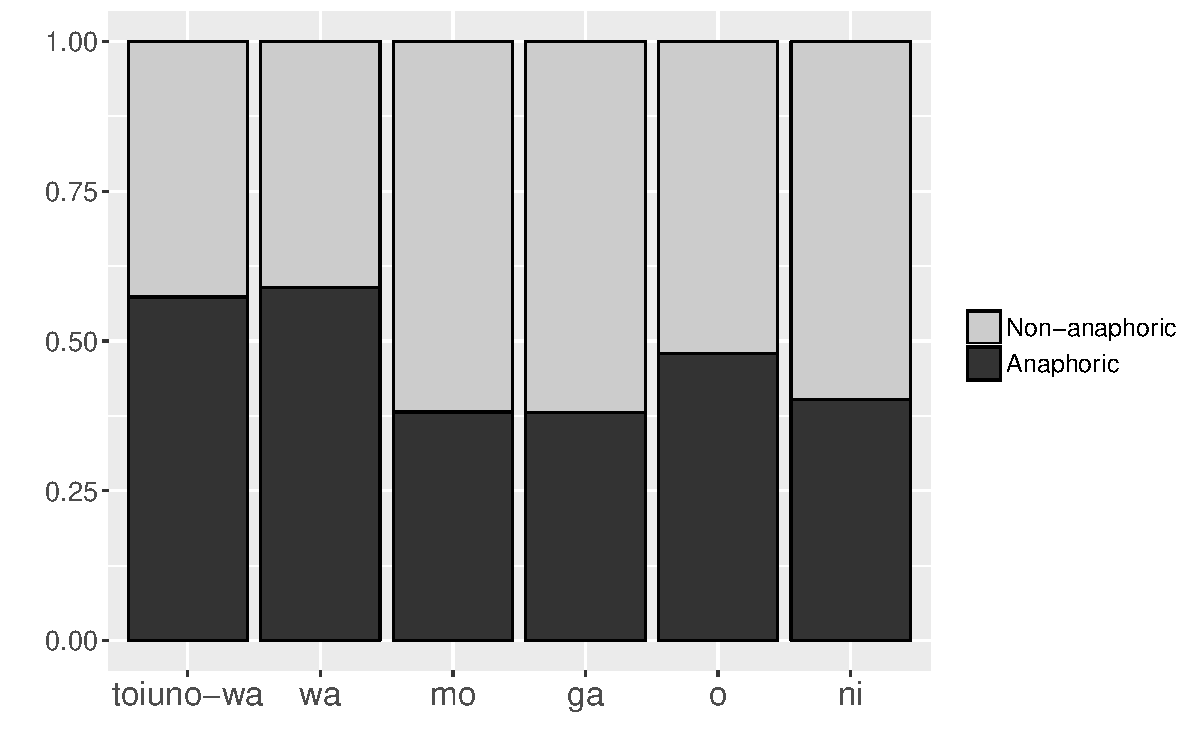
\includegraphics[width=0.8\textwidth]{figure/ParInfoStatus.pdf}
  \caption{Particle vs.\ information status (ratio)}
  \label{ParInfoStatusCTF}
\end{center}
\end{figure}

\begin{table}
 \begin{center}
 \tblcaption{\chd{The results of pairwise comparison among the least-squares means (information status)}}
 \label{Par:InfoStatusPar:LSMEANST}
 \begin{tabular}{lrrrrr}
 \toprule
 contrast      &    estimate &        SE & z.ratio & p.value & \\
 \midrule
  ga - o         & $-0.465$ & $0.149$ & $-3.120$ &  $0.022$ & * \\
  ga - wa        & $-0.748$ & $0.182$ & $-4.096$ & $<0.001$ & *** \\
  ga - toiuno-wa & $-0.659$ & $0.274$ & $-2.409$ &  $0.153$ &  \\
  o - wa         & $-0.282$ & $0.193$ & $-1.463$ &  $0.688$ &  \\
  o - toiuno-wa  & $-0.194$ & $0.282$ & $-0.688$ &  $0.983$ &  \\
  ni - wa        & $-0.661$ & $0.184$ & $-3.602$ &  $0.004$ & ** \\
  wa - toiuno-wa & $ 0.089$ & $0.293$ & $ 0.302$ &  $1.000$ &  \\
  wa - mo        & $ 0.759$ & $0.244$ & $ 3.107$ &  $0.023$ & * \\
 \bottomrule
 \end{tabular}
 \end{center}
\hfill{(0 $\le$ `***' $\le$ 0.001 $\le$ `**' $\le$ 0.01 $\le$ `*' $\le$ 0.05 `.' $\le$ 0.1 $\le$ ` ' 1)}
\end{table}

\begin{table}
	\begin{center}
	\tblcaption{Particle vs.~persistence}
	\label{ParPerNumT}
	\begin{tabular}{lrrrrrr}
	\toprule
	                  & \ci{toiuno-wa} & \ci{wa} & \ci{mo} & \ci{ga} & \ci{o} & \ci{ni} \\
	\midrule
	Persistent        & 45             & 107     & 53      & 209    & 175 & 184 \\
	                  & {\rt (66.2\%)} & {\rt (56.3\%)} & {\rt (44.9\%)} & {\rt (46.2\%)} & {\rt (51.5\%)} & {\rt (41.3\%)} \\
	Non-persistent    & 23             & 83     & 65      & 243    & 165 & 261 \\
	                  & {\rt (33.8\%)} & {\rt (43.7\%)} & {\rt (55.1\%)} & {\rt (53.7\%)} & {\rt (48.5\%)} & {\rt (58.7\%)} \\
	\midrule
	Sum               & 68             & 190     &  118    & 452    & 340 & 445 \\
	                  & {\rt (100\%)} & {\rt (100\%)} & {\rt (100\%)} & {\rt (100\%)} & {\rt (100\%)} & {\rt (100\%)} \\
	\bottomrule
	\end{tabular}
	\end{center}
\end{table}

\begin{figure}
%\begin{minipage}{0.5\textwidth}
	\begin{center}
	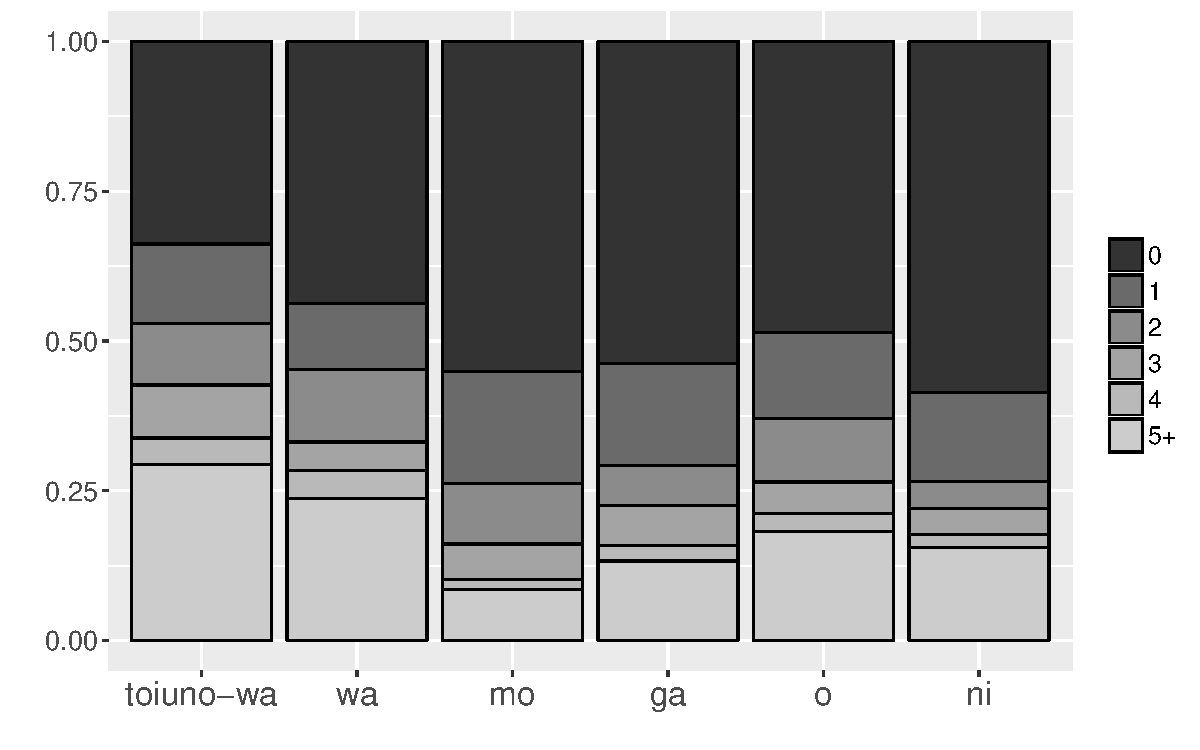
\includegraphics[width=0.8\textwidth]{figure/ParPerNum.pdf}
	\caption{Particle vs.\ \# of mention (ratio)}
	\label{ParPerNumF}
	\end{center}
\end{figure}
%\end{minipage}
%\begin{minipage}{0.5\textwidth}
%	\begin{center}
%	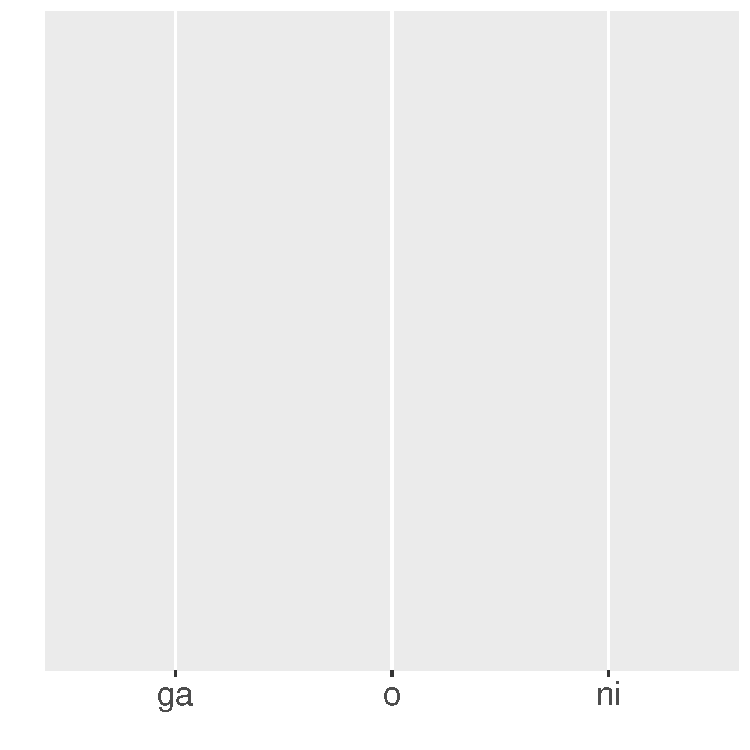
\includegraphics[width=0.95\textwidth]{figure/PerNumCasePar.pdf}
%	\caption{Case marker vs.\ \# of mention (ratio)}
%	\label{PerNumCaseParF}
%	\end{center}
%\end{minipage}

\begin{table}
 \begin{center}
 \tblcaption{\chd{The results of pairwise comparison among the least-squares means (persistence)}}
 \label{Par:PersistencePar:LSMEANST}
 \begin{tabular}{lrrrrr}
 \toprule
 contrast      &    estimate &        SE & z.ratio & p.value & \\
 \midrule
 ga - o         &  $-0.215$ & $0.146$ & $-1.473$ & $0.6817$ & \\
 ga - wa        &  $-0.349$ & $0.178$ & $-1.960$ & $0.3657$ & \\
 ga - toiuno-wa &  $-0.802$ & $0.281$ & $-2.856$ & $0.0491$ & * \\
 o - wa         &  $-0.134$ & $0.187$ & $-0.714$ & $0.9804$ & \\
 o - toiuno-wa  &  $-0.587$ & $0.287$ & $-2.044$ & $0.3171$ & \\
 o - ni         &  $ 0.440$ & $0.148$ & $ 2.978$ & $0.0345$ & * \\
 ni - wa        &  $-0.574$ & $0.180$ & $-3.189$ & $0.0179$ & * \\
 ni - toiuno-wa &  $-1.027$ & $0.282$ & $-3.642$ & $0.0037$ & ** \\
 wa - toiuno-wa &  $-0.453$ & $0.302$ & $-1.501$ & $0.6635$ & \\
 \bottomrule
 \end{tabular}
 \end{center}
 \hfill{(0 $\le$ `***' $\le$ 0.001 $\le$ `**' $\le$ 0.01 $\le$ `*' $\le$ 0.05 `.' $\le$ 0.1 $\le$ ` ' 1)}
\end{table}


Elements coded by so-called topic markers cannot be repeated as news as shown in hypothetical conversation between A and B in the following examples.
%
%	\ex. \ag. tozan-\EM{toiuno-wa} \\
%			mountain.climbing-\ab{quot}-\ci{wa} \\
%			`Mountain climbing is,'
%		\bg. ee yama-o nobot-te \\
%			\ab{fl} mountain-\ab{acc} climb-and \\
%			`(you) climb a mountain and'
%		\bg. tyoozyoo-ni tat-te \\
%			top-\ab{loc} stand-and \\
%			`(you) stand at the top of the mountain and'
%		\bg. soko-kara ee kudaru-toiu hitotu-no katee-ga aru-n-desu-keredomo \\
%			there-from \ab{fl} climb.down-\ab{quot} one-\ab{gen} process-\ab{nom} exist-\ab{nmlz}-\ab{cop}.\ab{plt}-though \\
%			`(you) climb down from there.' \hfill{(\code{S01F0151: 64.14-72.42})}
%		
%	\ex. hee, \{\EM{??tozan} / \}
%登山というのはえー山を登って
%頂上に立って
%そこからえー下るという一つの過程があるんですけれども (S01F0151: 64.14-72.42)
As in \Next and \NNext,
the \ci{toiuno-wa}-coded elements
\ci{mooningu thii} `morning tea'%
	\footnote{
	As discussed in \S \ref{Toiunowa},
	there are some formal variations of \ci{toiuno-wa} and,
	\ci{tteno-wa} is one of these variations.
	}
and \ci{eberesuto-kaidoo} `the Everest Trail'
cannot be repeated as news,
while the case-marker-coded elements \ci{kootya-ka koohii-ka} `tea or coffee', \ci{tibetto} `Tibet', \ci{nepparu} `Nepal', and \ci{kooeki-ro} `trading road'
can be repeated as news.
%
	\ex. \a.[A:] \ag. kono \EM{mooningu-thii-tteno-wa} \\
			this morning-tea-\ci{toiuno}-\ci{wa} \\
			`(In) this morning tea (time)'
		\bg. ma \EM{kootya-ka} \EM{koohii-ka-tteiuno-o} erab-eru-n-desu-keredomo \\
			\ab{fl} black.tea-or coffee-or-\ab{quot}-\ci{o} choose-can-\ab{nmlz}-\ab{plt}-though \\
			`(you) can choose tea or coffee.'
			 \hfill{(\code{S01F0151: 297.23-300.44})}
		\z.	
	\b.[B:] hee, \{\EM{??moo-ningu-thii(-wa)}/ \EM{kootya-ka koohii-o}\}\\
			Oh, \{morning tea/tea or coffee\}
	

%このモーニングティーってのはま紅茶かコーヒーかっていうのを選べるんですけれども (S01F0151: 297.23-300.44)
%
	\ex. \a.[A:] \ag. kono \EM{eberesuto-kaidoo-toiuno-wa} \\
			this Everest-road-\ab{quot}-\ci{wa} \\
			`This Everest Trail is'
		\bg. \EM{tibetto-to} \EM{nepaaru-no} \EM{kooeki-ro-ni}-mo nat-te ori-masi-te \\
			Tibet-and Nepal-\ab{gen} trade-road-for-also  become-and \ab{plt}-\ab{plt}-and \\
			`also used for trading between Tibet and Nepal.'
			 \hfill{(\code{S01F0151: 105.73-110.29})}
		\z.
	\b.[B:] hee, \{\EM{??eberesuto-kaidoo(-wa)}/\EM{tibetto-to}/\EM{nepaaru-to} / \EM{kooeki-ro-ni(-mo)}\}\\
			Oh, \{Everest Trail/Tibet/Nepal/trading road\}
	

%このエベレスト街道というのはチベットとネパールの交易路にもなっておりまして (S01F0151: 105.73-110.29)
%
As shown in \Next,
the element \ci{thii-taimu} `tea time' coded by copula + \ci{kedo}%
	\footnote{
	Again there are some variations of this marker
	and I will discuss this in \S \ref{kedo}.
	}
or the \ci{wa}-coded element \ci{takai tokoro} `places of high elevation'
cannot be repeated as news,
while the \ci{ga}-coded elements can be repeated as news.
%
\ex. \a.[A:] \ag. de kono \EM{thii-taimu-nan-desu-keredomo} \\
		and this tea-time-\ab{nmlz}-\ab{cop}.\ab{plt}-though \\
		`And at this tea time,'
	\bg. kono hyookoo-no \EM{takai} \EM{tokoro-de-wa} koozanbyoo-toiu hizyooni \EM{kikennna} \EM{kanoosee-ga} aru-node \\
		this elevation-\ab{gen} high place-\ab{loc}-\ci{wa} altitude.sickness-\ab{quot} very dangerous possibility-\ab{nom} exist-because \\
		`this place of high elevation, there is a possibility of altitude sickness, so...'
	\bg. ee \EM{mizu-ga} hizyooni zyuuyooni nari-masu \\
		\ab{fl} water-\ab{nom} very important become-\ab{plt} \\
		`water is very important.'
		 \hfill{(\code{S01F0151: 339.78-349.56})}
	\z.
\b.[B:] hee, \{\EM{??thii-taimu}/\EM{??takai tokoro-de}/\EM{kikennna kanoosee-ga}/\EM{mizu-ga}\} \\
	Oh, \{tea time/on places of high elevation/the possibility of danger/water\}


%でこのティータイムなんですけれども
%この標高の高いところでは高山病という非常に危険な可能性があるので
%えー水が非常に重要になります (S01F0151: 339.78-349.56)
%
%僕らそのー新人で入った時っていうのは
%一応新人いー用にあまある程度残業代ってのが確保されてるらしいんですね (S05M1236: 393.59-401.15)
%
%On the other hand,
%\ci{mo}-coded elements can be repeated as news
%as shown in \Next.
%%
%\ex.\label{kosobo-tiiki-de-mo}
% \a.[A:]
% \ag. kono \EM{kosobo-tiiki-de-mo} \\
% 	this Kosovo-region-\ab{loc}-also \\
%	`Also in this Kosovo,'
% \bg. minzoku-hunsoo-ga okot-ta wake-de-gozaimasu-ga \\
% 	ethnic-conflict-\ci{ga} happen-\ab{past} reason-\ab{cop}-\ab{plt}-though \\
%	`ethnic conflicts occurred, and...'
%	\hfill{(\code{S00M0199: 163.04-165.91})}
% \z.
% \b.[B:] hee, \{$^{ok}$kosobo-tiiki-de(-mo)/minzoku-hunsoo-ga\} \\
% 	Oh, \{(also) in Kosovo/ethnic conflicts\}.
%
%このコソボ地域でも
%民族紛争が起こった訳でございますが
% (S00M0199: 163.04-165.91)
%
%According to Figure \ref{TopParInfoStatusF} and Table \ref{TopParInfoStatusT},
%more than half of the \ci{mo}-coded elements are new,
%and, according to Figure \ref{PerNumTopParF} and Table \ref{PerNumTopParT},
%approximately half of the \ci{mo}-coded elements are non-persistent.
%Based on our criteria for topic,
%\ci{mo}-coded elements are not topics.
%The characteristics of elements coded by \ci{mo} `also' will be discussed in \S \ref{Mo}.
%Basically \ci{mo} codes an element
%in addition to some set that has already been introduced.

As indicated in Table \ref{ParInfoStatusT} and will be discussed below,
brand-new elements can never be coded by topic markers;
they can never be assumed to be shared between the speaker and the hearer.
Non-anaphoric elements coded by topic markers are
inferable, declining, or unused
as will be discussed in the following sections.
%as has been pointed out in \citeA{kuno73} and as has been discussed in \S \ref{BackSecTopic}.
For example,
as in \Next,
it is unacceptable for topic markers to code brand new elements \ci{oozei-no hito} `many people' out-of-the-blue.
% without assuming that the hearer can identify which girl the speaker is talking about.%
%	\footnote{
%	As discussed in \S \ref{TopZero} and \S \ref{FocZero},
%	the agent-like argument of transitive clauses can be zero-coded if it is a topic,
%	while it cannot if it is (part of) a focus.
%	Hence the zero markers that code \ci{oozei-no hito} `many people' in \Next and \ci{otoosan} `father' in \NNext are unambiguously interpreted as topic zero marker.
%	}
%
\exg.
 *\EM{oozei-no} \EM{hito-wa} paathii-ni ki-masi-ta \\
  many-\ab{gen} person-\ci{wa} party-\ab{dat} come-\ab{plt}-\ab{past} \\
  `Speaking many people, they came to the party.'
    \hfill{\cite[~45]{kuno73}}
% \bg. *dareka-\EM{wa} byooki-desu \\
%       somebody-\ci{wa} sick-\ab{cop}.\ab{plt}\\
%       `Speaking of somebody, he is sick.'
%       \hfill{(ibid.)}

Similarly, it is unacceptable for other topic markers to code these elements, whereas \ci{ga} can code them.
%
\exg.
 \EM{oozei-no} \EM{hito-\{??{toiuno-wa}/??da-kedo/??{\O}/ga\}} paathii-ni ki-masi-ta \\
 many-\ab{gen} person-{\{\ci{toiuno-wa}/\ab{cop}-\ci{though}/{\O}/\ci{ga}\}} party-\ab{dat} come-\ab{plt}-\ab{past} \\
 `Many people came to the party.'
% \bg. dareka-\{??{toiuno-wa}/??wa/??da-kedo/??{\O}/ga\} ki-masi-ta-ne \\
%       somebody-\{\ci{toiuno-wa}/\ci{wa}/\ab{cop}-\ci{though}/{\O}/\ci{ga}\} come-\ab{plt}-\ab{past}-\ab{fp} \\
%       `Somebody came.'


%\exg. a! \label{onnanoko}\EM{onnanoko-\{??{toiuno-wa}/??wa/??da-kedo/??{\O}/ga\}} henna boosi kabut-temasu-yo \\
% oh! girl-\{\ci{toiuno-wa}/\ci{wa}/\ab{cop}-\ci{though}/{\O}/\ci{ga}\} weird hat wear-\ab{prog}.\ab{plt}-\ab{fp} \\
% `A girl is wearing a red hat.' 

%Although it is possible to interpret \Last as ``girls in general wear red hats,''
%it is otherwise unacceptable.
While \ci{oozei-no hito} `many people' in \Last was unanchored in Prince's term,
\ci{taroo-no otoosan} `Taro's father' in \Next is anchored.
The element coded by a topic marker is still not acceptable in an out-of-the-blue context.
%
\exg. a! \EM{taroo-no} \EM{otoosan-\{??{toiuno-wa}/??wa/??da-kedo/{\O}\}} asoko-de tabako sut-teru-yo \\
 oh! Taro-\ab{gen} father-\{\ci{toiuno-wa}/\ci{wa}/\ab{cop}-\ci{though}/{\O}\} there-\ab{loc} cigarette smoke-\ab{prog}.\ab{plt}-\ab{fp} \\
 `Taro's father is smoking over there.'

Therefore, topic markers in Japanese are sensitive to the given-new taxonomy rather than definiteness and identifiability.%
 \footnote{
 I suppose that the zero particle is acceptable
 because the zero particle in this case is ambiguous between topic and focus coding.
 }

Finally, as will be discussed in detail in \S \ref{TopZero},
an element coded by a zero particle ({\O}) that precedes other arguments and is uttered in a coherent intonation contour
cannot be repeated as news and hence considered to be presupposed to be shared.
\ex. \label{mouse}Context: Y and H are roommates,
	who are bothered by a mouse running around their room
	and eating their leftovers.
	The cat they keep finally caught the mouse while H was out.
	When H is back, Y wants to let H know this news.
	\ag.[Y:] \EM{nezumi-\O} neko-ga tukamae-ta-yo \\
		nezumi-{\O} cat-\ci{ga} catch-\ab{past}-\ab{fp} \\
		`The cat caught (the) mouse.'
	\b.[H:] hee, \{??nezumi, neko(-ga)\} \\
	  Oh, \{mouse, cat(-\ci{ga})\}
	  \hfill{(=\ref{FrameworkExMouse} in \S \ref{FrameworkTopic})}


In the following sections,
I analyze each topic markers in detail.

%%----------------------------------------------------
\subsection{\textit{Toiuno-wa}}\label{Toiunowa}

In this section
I will show that \ci{toiuno-wa} codes elements of referents
which are evoked
through explicit or implicit introduction of the elements or
availability in the universe of discourse.

There are phonetic variations of \ci{toiuno-wa}:
\ci{(t)teno-wa}, \ci{t(y)uuno-wa}, \ci{teiuno-wa}, etc.
I put them into the same category \ci{toiuno-wa} and assume that they are the same
except for stylistic difference.


%%----------------------------------------------------
\subsubsection{Evoked elements tend to be coded by \textit{toiuno-wa}}

\ci{Toiuno-wa} typically codes evoked elements.
As exemplified in \Next and \NNext,
the antecedent of the \ci{toiuno-wa}-coded elements,
\ci{un} `fortune' in \Next and \ci{tiryoo-hoo} `treatment methods' in \NNext,
are mentioned in the immediately preceding contexts.
%
\ex.
 \ag. syokugyoo-ni taisite-no \EMi{un}-toiu koto-o tyotto o-hanasi si-tai-to omoi-masu \\
		job-to towards-\ab{gen} fortune-\ab{quot} thing-\ci{o} a.bit \ab{plt}-talk do-want-\ab{quot} think-\ab{plt} \\
		`I would like to talk a bit about fortune in job.'
 \bg. de \EM{un-toiuno-wa} maa iroirona un-ga aru-to omou-n-desu-keredomo \\
 	then fortune-\ci{toiuno-wa} \ab{fl} various fortune-\ci{ga} exist-\ab{quot} think-\ab{nmlz}-\ab{plt}-though \\
	`I guess there are various kinds of fortunes...'
	\hfill{(\code{S01F0038: 0.53-8.70})}
%職業に対しての運ということをちょっとお話ししたいと思います
%で運というのはまー色々な運があると思うんですけれども
%(S01F0038: 0.53-8.70)

\ex. \ag. de sono byooki-wa gen'in-ga humee-de \\
	and that disease-\ci{wa} source-\ci{ga} unknown-\ab{cop} \\
	`And the source of that disease was unknown, and'
	\bg. \EMi{tiryoo-hoo}-mo kakuritu-si-tei-mas-en-desi-ta \\
		treatment-method-also establish-do-\ab{pfv}-\ab{plt}-\ab{neg}-\ab{plt}-\ab{past} \\
		`The treatment methods had not been established.'
	\bg. sono \EM{tiryoo-hoo-toiuno-wa} yuiitu ... suteroidozai-de sinkoo okur-aseru koto-dake-desi-ta \\
		that treatment-method-\ci{toiuno-wa} only ... steroid-by progress delay-\ab{caus} thing-only-\ab{plt}-\ab{past} \\
		`The only way to treat is just to delay the progress of the disease by steroid that I cannot use.' \hfill{(\code{S02F0100: 294.39-308.12})}

%でその病気は原因が不明で治療法も確立していませんでした
%その治療法というのは唯一私が使うことのできないステロイド剤で進行遅らせることだけで (S02F0100: 294.39-308.12)

Non-anaphoric elements coded by \ci{toiuno-wa} are considered to be evoked
through implicit introduction of an element or by the physical context.
In \Next,
\ci{supootu-kansen} `sport watching' is non-anaphoric
but the speaker mentioned that he watched a world title match.
Thus `sport watching' is considered to be evoked
when the speaker mentioned `sports watching' with \ci{toiuno-wa} coding in line c.
%
\ex. \ag. ee \EMi{sekai-taitoru-sen-o-desu-ne} ee \EMi{terebi-de} \EMi{mi-masi-ta} \\
		\ab{fl} world-title-fight-\ci{o}-\ab{plt}-\ab{fp} \ab{fl} TV-by watch-\ab{plt}-\ab{past} \\
		`(My friend and I) watched a world title match on TV.'
	\b. ...
	\bg. watasi-zisin gu -wa ee amari koo \EM{supootu-kansen-teiunowa} tyotto si-nakat-ta-n-desu-ne \\
		\ab{1}\ab{sg}-self \ab{frg} -\ci{wa} \ab{fl} not.really \ab{fl} sport-watching-\ci{toiuno-wa} \ab{fl} do-\ab{neg}-\ab{past}-\ab{nmlz}-\ab{plt}-\ab{fp} \\
		`I myself hadn't watched any kinds of sports.' \hfill{(\code{S01M0182: 52.77-79.62})}
%	
%えー世界タイトル戦をですねえーテレビで見ました
%...
%私自身ぐはえーあまりこうスポーツ観戦ていうのはちょっとしなかったんですね (S01M0182: 52.77-79.62)

Similarly, in \Next,
\ci{taitoru} `title (in piano competitions)' is an non-anaphoric element
but the speaker was talking about `awards' in the preceding context
and `title' can be considered to have been evoked at the time of utterance \Next[e].
%
\ex. \a. I have been participating in various piano competitions
	\b. So far the best award I received was the fourth best play in the China-Japan International Competition.
	\b. Beyond that, I would like to receive higher awards.
	\bg. ano doositemo kore-wa yappari piano-o kokorozasu mono-ni totte-wa \\
		\ab{fl} anyhow this-\ci{wa} anyway piano-\ci{o} orient people-for in.terms.of-\ci{wa} \\
		`This, for those who want to make name as a pianist,'
	\bg. kono \EM{taitoru-tteiuno-wa} sugoku ookii-node \\
		this title-\ci{toiuno-wa} very big-because \\
		`titles matters a lot, so...'
\hfill{(\code{S00F0209: 507.13-529.76})}
%
%やはりあの今まで受けたコンクールの最高順位が
%あのま日中友好国際音音楽コンクールっていうのがあって
%それがまー一般のピアノ部門で四位で奨励賞だったんですね
%でそれを超えてあの三位以内に入賞することがまず一つで
%あのどうしてもこれはやっぱりピアノを志す者にとっては
%このタイトルってのは凄く大きいので (S00F0209: 507.13-529.76)

In another example like \Next,
\ci{toiuno-wa}-coded elements are considered to be evoked through ``common sense''.
\Next is the beginning of the talk
but the speaker mentions \ci{ningen} `human being' with \ci{toiuno-wa} coding.
This is because
people can always talk about human beings even in out-of-the-blue contexts.
Therefore, ``human beings'' are always available as topic.
\ci{Tuuno-wa} is a variation of \ci{toiuno-wa}.
%the human being is always evoked through the physical context.
%
\exg.\label{ExNingenToiunowa}\EM{ningen-tuuno-wa} hizyooni ano umaku deki-teru doobutu-da-to omoi-masu-ne \\
	human-\ci{toiuno-wa} very \ab{fl} well created-\ab{pfv} animal-\ab{cop}-\ab{quot} think-\ab{plt}-\ab{fp} \\
	`I think that human beings are well-created.' \\
 \hfill{(\code{S02M1698: 6.99-11.00})}
%
%人間つうのは非常にあのうまくできてる動物だと思いますね (S02M1698: 6.99-11.00)

Readers might think that \Last is acceptable because `human being' is generic rather than evoked in the physical context.
However, I do not employ this account for the following two reasons:
(i) being generic is a characteristics across all \ci{toiuno-wa}-coded elements (see \S \ref{Par:Topic:Toiunowa:Other}), and
(ii) even though the elements are generic, some elements are still difficult to be coded by \ci{toiuno-wa} in the beginning of speeches.
%Let us discuss example \Next, which is at the very beginning of a speech about Kosovo conflicts.
\chd{Let us discuss example \Next,
which is at the very beginning of a speech about travel to Hawaii.}
%
\exg.\label{Par:Toiunowa:Ex:Hawaii}teema-wa hawai-too-no sizen-no subarasisa-to tabi-no tanosisa-nituite-desu \\
   theme-\ci{wa} Hawaii-island-\ab{gen} nature-\ab{gen} splendor-and travel-\ab{gen} fun-about-\ab{cop} \\
   `The topic (of this talk) is about the splendor of Hawaii nature and fun of travelling.'
 \hfill{(\code{S00F0014: 0.30-6.08})}
%テーマはハワイ島の自然の素晴らしさと旅の楽しさについてです
%%
%\ex.\label{ExKosovo}
% \ag. ee \ci{kosobo-mondai}-ni-tuite \\
%	\ab{fl} Kosovo-problem-on-about \\
%	`On Kosovo conflicts.'
% \bg. ee ima-kara tyoodo ee iti-nen-hodo-mae-ni nari-masu-ne \\
% 	\ab{fl} now-from exactly \ab{fl} one-year-ago-about-to become-\ab{plt}-\ab{fp} \\
%	`From now, it was exactly a year ago...'
%	\hfill{(\code{S00M0199: 0.24-10.50})}
%%えーコソボ問題について
%%えー今からちょうどえー一年程前になりますね
%% (S00M0199: 0.24-10.50)

\chd{In this example,
the speaker did not choose to code `the splendor of Hawaii nature and fun of travelling' with \ci{toiuno-wa}.
It is harder to code this with \ci{toiuno-wa} than `human being' because
it is not always available as topic
even though `the splendor of Hawaii nature and fun of travelling'
is generic.}
%The sentence itself is natural if \ci{ni-tuite} is replaced with \ci{toiuno-wa}.
%(In that case, \Last[a-b] are considered to be a single coherent sentence.)
%However, it is slightly unnatural without introducing `Kosovo conflict'
%in the preceding discourse.
Therefore,
I argue that the acceptability of \ci{toiuno-wa} coded `human being' without introduction of human beings in \LLast is possible
because it is always available as topic,
not because it is generic.


%%----------------------------------------------------
\subsubsection{Declining or inferable elements tend not to be coded by \textit{toiuno-wa}}\label{Toiuno-waInfSemiActUnuse}

There are a few examples
where \ci{toiuno-wa} codes inferable elements.
In \Next,
the speaker explains why she came to Iran and describes the middle school there.
The climate in Iran has not been mentioned before \Next[c],
but is still coded by \ci{toiuno-wa}.
The climate in Iran is neither implicitly introduced nor available as universal topic.
\ex. \label{IranClimate}
 \a. (The speaker moved to Iran when she is a middle school student.)
 \b. (The school for Japanese students in Iran was small but she had a lot of fun there.)
 \bg. eeto iran-no \EM{kikoo-tteiuno-wa} tomokaku kansoo si-tei-masi-te \\
 	\ab{fl} Iran-\ab{gen} \ci{climate-toiuno-wa} at.any.rate dry do-\ab{prog}-\ab{plt}-and \\
	`Uh, the climate in Iran was very dry...'
	\hfill{(\code{S03F0072: 178.31-181.65})}
%えーとイランの気候っていうのはともかく乾燥していまして
% (S03F0072: 178.31-181.65)
%

Similarly, in \Next[c],
the speaker is going to talk about a dog his family kept.
The speaker begins with the explanation why the dog came to his house.
The element \ci{keei} `background (of why the dog came)' is coded by \ci{toiuno-wa},
although \ci{keei} has not been explicitly mentioned in the preceding context.
%
\ex.
 \a. (The speaker talks about a dog his family kept.)
 \b. (After the death of the previous dog they kept, the dog he is going to talk about joined his family.)
 \bg. e uti-ni ki-ta \EM{keei-toiuno-wa} \\
 	\ab{fl} home-to come-\ab{past} background-\ci{toiuno-wa} \\
	`The background of how the dog came to our house is'
 \bg. ma sono zyuui-san-no syookai-nan-desu-keredomo \\
 	\ab{fl} that vet-\ab{hon}-\ab{gen} introduction-\ab{nmlz}-\ab{cop}.\ab{plt}-though \\
	`(through) the introduction of that vet...'
	\hfill{(\code{S02M0198: 141.97-146.92})}
%えうちに来た経緯というのは
%まその獣医さんの紹介なんですけれども
% (S02M0198: 141.97-146.92)


On the other hand,
there are some cases where it is unnatural for \ci{toiuno-wa} to code inferable elements.
For example, in \Next[c],
the element \ci{hikoozyoo} `airport' cannot naturally be coded by \ci{toiuno-wa},
which is originally coded by \ci{wa}.
The airport is inferable because the speaker has already mentioned flying to Lukla.
\ex.
%
%		\ag. hikooki-de ee hyookoo 2600 meetoru-no rukura-to iu mura-ni mazu tobi-masu \\
%			airplane-by \ab{fl} elevation 2600 meter-\ab{gen} Lukla-\ab{quot} call village-to first fly-\ab{plt} \\
	\a. To start Himalaya trekking, you first fly to a village called Lukla whose elevation is 2600 meters.
%		\bg. soko-kara ee torekkingu-o kaisi-itasi-masi-ta \\
%			that-from \ab{fl} trekking-\ab{acc} start-do-\ab{plt}-\ab{past} \\
	\b. From that village, we started trekking.
	\bg. sono rukura-no mura-nan-desu-ga \\
		that Lukla-\ab{gen} village-\ab{nmlz}-\ab{plt}-though \\
		`Regarding that Lukla village,'
	\bg. \EM{hikoozyoo-\{wa}(/??-\EM{toiuno-wa})\} hontooni yama-no naka-ni ari-masi-te \\
		airport-\ci{wa}(/-\ci{toiuno-wa}) really mountain-\ab{gen} inside-in exist-\ab{plt}-and \\
		`the airport is really in a mountainous area.'
	\hfill{(\code{S01F0151: 179.50-191.39})}
%飛行機でえー標高二千六百メートルのルクラという村にまず飛びます
%そこからえートレッキングを開始いたしました
%そのルクラの村なんですが
%飛行場は本当に山の中にありまして (S01F0151: 179.50-191.39)

I speculate that the different acceptabilities of \ci{toiuno-wa} among \ref{IranClimate}, \LLast, and \Last are due to different statuses of given-new taxonomy or the accessibility of the elements;
`the climate' in \ref{IranClimate} and `the background' in \LLast are more general terms and are easily accessible
than `the airport' in \Last.
Note that this does not contradict, rather, is consistent with, the Semantic Map connectivity Hypothesis \ref{SemanticMapHypIS}.
Since the given-new taxonomy scale is continuous,
the boundary between evoked and inferable is blur, and
among the inferable elements in these examples,
`the climate' of Iran in \ref{IranClimate} and `the background' in \LLast are easier to access than `the airport' in \Last.
This is consistent with the nature of the conceptual space,
although the boundary is drawn clearly in the semantic map in Table \ref{ParInfoStatusT}
for the purpose of presentation.

It is unnatural when \ci{toiuno-wa} codes declining elements.
The degree of how a referent is declining is difficult to calculate from the corpus.
Apparently, it does not simply correspond to the distance between an element and its antecedent,
but the intervention of (an)other topic(s) seems to be more relevant.
For example,
a copula followed by \ci{kedo} codes declining or unused elements as will be shown in \S \ref{kedo}.
In \Next[g],
it codes a declining element rather than unused element
because the element has already been introduced in line a.
In line a, two potential topics `fame' and `job' are introduced.
The speaker talks about `fame' first and moves on to `job' in line g.
It is fair to assume that the topic `job' is intervened by another topic `fame'.
When the element `job' is retrieved as a current topic in line g,
it is coded by a copula followed by \ci{keredomo} `though',
a variation of \ci{kedo}.
However,
this marker cannot be replaced with \ci{toiuno-wa}.
%
\ex.\label{sigoto}
 \a. I have two goals: one is for \EMi{fame} and the other is for \EMi{\EMi{job}}.
 \b. Concerning \EMi{fame},
 \b. I have been participating in various piano competitions
 \b. So far the best award I received was the fourth best play in the China-Japan International Competition.
 \b. Beyond that, I would like to receive higher awards.
 \b. Titles matters a lot for pianists, so I will work hard.
 \bg. de ato-wa \EM{sigoto-no} \EM{bubun-\{nan-desu-keredomo/(??toiuno-wa)\}} \\
 	then remaining-\ci{wa} job-\ab{gen} part-\{\ab{nmlz}-\ab{cop}.\ab{plt}-though/\ci{toiuno-wa}\} \\
	`Concerning the other one, job,'
 \b. to receive higher wages...
\hfill{(\code{S00F0209: 495.77-539.19})}
%
%これからのあの目標っていうのがありまして
%まそれは大きく分けて二つあるんですけども
%ま名声の部分と仕事っていう部分がありまして
%一番目の名声の部分は
%やはりあの今まで受けたコンクールの最高順位が
%あのま日中友好国際音音楽コンクールっていうのがあって
%それがまー一般のピアノ部門で四位で奨励賞だったんですね
%でそれを超えてあの三位以内に入賞することがまず一つで
%あのどうしてもこれはやっぱりピアノを志す者にとっては
%このタイトルってのは凄く大きいので
%あのやってきたいです
%で後は仕事の部分なんですけれども
%あの一回のギャランティーがえーと勿論アップするように
% (S00F0209: 495.77-539.19)


%\begin{figure}
%\begin{minipage}{0.5\textwidth}
%	\begin{center}
%	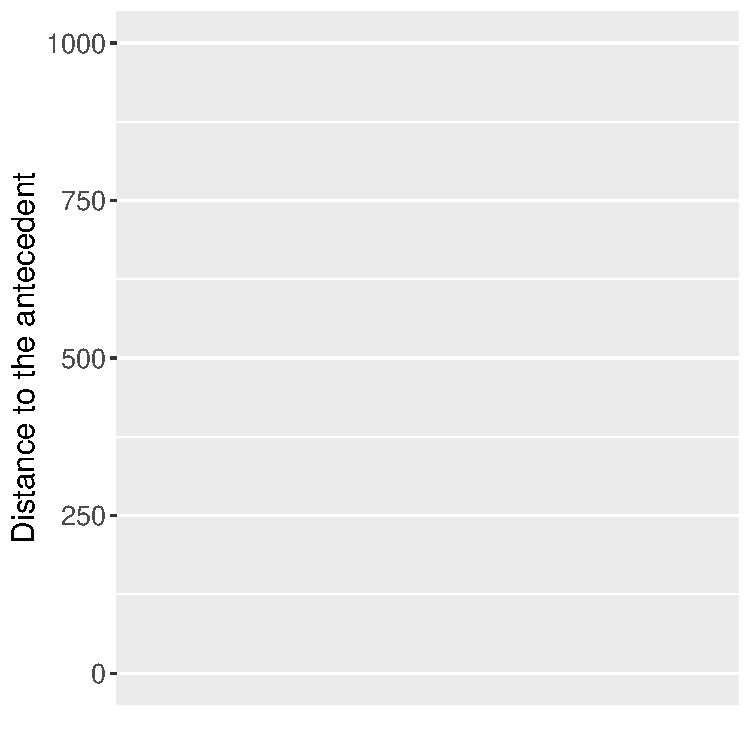
\includegraphics[width=0.95\textwidth]{figure/AnaRelDistTop.pdf}
%	\caption{}
%	\label{AnaRelDistTopF}
%	\end{center}
%\end{minipage}
%\begin{minipage}{0.5\textwidth}
%	\begin{center}
%	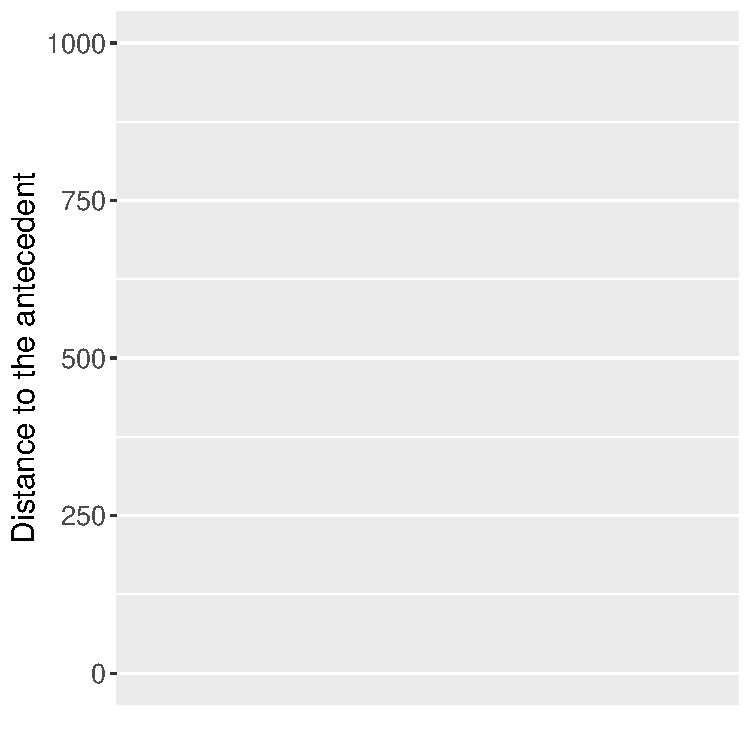
\includegraphics[width=0.95\textwidth]{figure/AnaRelDistCase.pdf}
%	\caption{}
%	\label{AnaRelDistCaseF}
%	\end{center}
%\end{minipage}
%\end{figure}



\ci{Toiuno-wa} cannot code elements that have not been established as topic.
In \Next,
although `tea time' is introduced in line b,
it does not appear to be established enough as topic,
which makes \ci{toiuno-wa} unnatural in line d;
the original marker is a copula followed by \ci{keredomo}.
%
\ex.\label{thii-taimu}
 \a. While we trek on the Everest Trail, the cook made us lunch on the way,
 \b. in addition, there is tea time and we can take a break while we climb the mountain,
 \b. so, we walked without feeling that we were in a big group.
 \bg. de kono \EM{thii-taimu-nan-desu-\{keredomo/(??toiuno-wa)\}} \\
		and this tea-time-\ab{nmlz}-\ab{cop}.\ab{plt}-\{though/toiuno-wa\} \\
		`And at this tea time,'
 \bg. kono hyookoo-no {takai} {tokoro-de-wa} koozanbyoo-toiu hizyooni {kikennna} {kanoosee-ga} aru-node \\
		this elevation-\ab{gen} high place-\ab{loc}-\ci{wa} altitude.sickness-\ab{quot} very dangerous possibility-\ci{ga} exist-because \\
		`this place of high elevation, there is a possibility of altitude sickness, so...'
 \bg. ee {mizu-ga} hizyooni zyuuyooni nari-masu \\
		\ab{fl} water-\ci{ga} very important become-\ab{plt} \\
		`water is very important.'
		 \hfill{(\code{S01F0151: 323.00-349.56})}
%途中でえー勿論お昼御飯もキッチンスタッフが作ってくれたり
%後はティータイムって言って
%途中でちょっとブレークする時間もあるんですけれども
%えーかなりえーそういうツアーで来ているっていう印象をそんなに与えないで
%えー歩くことができました
%でこのティータイムなんですけれども
%この標高の高いところでは高山病という非常に危険な可能性があるので
%えー水が非常に重要になります (S01F0151: 323.00-349.56)

These subtle differences of acceptability of \ci{toiuno-wa} cannot be captured simply by counting numbers.
However, they are clear from the acceptability judgements.

Unused elements also cannot be coded by \ci{toiuno-wa}.
It is very difficult to find unused elements
because of the nature of our corpus;
each speaker gave a speech in front of people s/he does not know
and there are few things the speaker can assume to be shared with the hearer(s).
However, constructed examples like \Next clearly shows that \ci{toiuno-wa} cannot code unused elements.
%
\ex. \label{FacebookParty}Context: According to Facebook, both A and B are going to a party tomorrow. But they have not seen each other for a week. A sees B in a classroom and talks to B:
	\a.[A:] asita-no \EM{paathii-\{da-kedo/??toiuno-wa\}} nan-zi-kara-na-no \\
		tomorrow-\ab{gen} party-\{\ab{cop}-though/\ci{toiuno-wa}\} what-o'clock-from-\ab{cop}-\ab{q} \\
		`What time does tomorrow's party start?' 

Note that if the element `party' has already been introduced into the discourse, \ci{toiuno-wa} can code it.
This is shown in \Next[A].%
	\footnote{
	In this example, I am using \ci{tteiuno-wa} instead of \ci{toiuno-wa}
	simply because this hypothetical utterance is casual;
	\ci{tteiuno-wa} is more casual than \ci{toiuno-wa}.
	\ci{Toiuno-wa} sounds too formal in this utterance.
	}
\ex. \label{Party}Context: A and B are having a conversation. B mentioned the tomorrow's party, which A knows that both A and B are going to.
	\ag.[A:] sono \EM{paathii-\{??da-kedo/tteiuno-wa\}} nan-zi-kara-na-no \\
		that party-\{\ab{cop}-though/\ci{toiuno-wa}\} what-o'clock-from-\ab{cop}-\ab{q} \\
		`What time does tomorrow's party start?' 


%%----------------------------------------------------
\subsubsection{Further characteristics of \textit{toiuno-wa}-coded elements}\label{Par:Topic:Toiunowa:Other}

Statements about \ci{toiuno-wa}-coded elements tend to represent the general characteristics of the referents
as has been pointed out in \citeA{masuoka87,masuoka08}.
Masuoka argues that \ci{toiuno-wa}-coded elements only accompany individual-level predicates (in his term, property predicates).
This is clearly shown in the contrast between \Next[a] and \Next[b] (repeated from \ref{ExSatiko}) in \S \ref{Back:GeneralChar:Toiunowa}.
Whereas the stage-level predication \Next[a] does not allow \ci{toiuno-wa},
the individual-level predication \Next[b] does allow \ci{toiuno-wa}.
%
\ex.
\ag. *satiko-\EM{toiuno-wa} uso-o tui-ta \\
     Sachiko-\ci{toiuno-wa} lie-\ci{o} commit-\ab{past} \\
     `Sachiko lied.'
     \hfill{\cite[p.~96]{masuoka12}}
\bg. satiko-\EM{toiuno-wa} uso-tuki-da \\
     Sachiko-\ci{toiuno-wa} lie-commiter-\ab{cop} \\
     `Sachiko is a liar.'
     \hfill{(Constructed)}

In our corpus,
most examples of \ci{toiuno-wa} also accompany individual-level predication
rather than stage-level predication.
In \Next,
the speaker is talking about the general characteristics of puppies.
%
\exg. \EM{koinu-toiuno-wa} dono syurui-demo hizyooni ano neru-no-ga tokui-desu-ne \\
 puppy-\ci{toiuno-wa} which kind-also very \ab{fl} sleep-\ab{nmlz}-\ci{ga} good.at-\ab{cop}.\ab{plt}-\ab{fp} \\
 `Puppies are, no matter what kinds, good at sleeping.'
 \hfill{(\code{S02M1698: 166.62-170.59})}
%小犬というのはどの種類でも非常にあの寝るのが得意ですね
% (S02M1698: 166.62-170.59)

The explanation for this requires further investigation.

%As exemplified in the contrast between \Next[b] and \Next[b$^{\prime}$],
%\ci{toiuno-wa} can be used when the statement is about the usual event for the cat,
%while it cannot when the statement is about the event that happened only once.
%%
%\ex.
% \a. I had a cat when I was small.
% \bg. sono \EM{neko-toiuno-wa} yoku mado-no soto-o mi-tei-masi-ta \\
% 	that cat-\ci{toiuno-wa} often window-\ab{gen} outside-\ci{o} look-\ab{prog}-\ab{plt}-\ab{past} \\
%	`The cat was often looking at the outside of the window...'
% \bg.[b$^{\prime}$.] aru hi watasi-ga gakkoo-ni iku toki sono \EM{neko-\{??toiuno-wa/wa\}} mado-no soto-o mi-tei-masi-ta \\
% one day \ab{1}\ab{sg}-\ci{ga} school-to go when that cat-\{\ci{toiuno-wa}/\ci{wa}\} window-\ab{gen} outside-\ci{o} look-\ab{prog}-\ab{plt}-\ab{past} \\
% `One day, when I was going to school, the cat was looking at the outside of the window...'
 


%\ex. 
% \a. kitee-ga ari-masi-te \\
% 	rule-\ci{ga} exist-\ab{plt}-and \\
%	`There is a rule (for collecting debts from people),'
% \b. n o sono \EM{kaisyuu-rinri-kitee-tteiuno-wa} \\
% 	\ab{fl} \ab{fl} collect-ethic-rule-\ci{toiuno-wa} \\
%	`the rule'
% \b. ironna koomoku-de takusan ume-rare-te-desu-ne \\
% 	various point-with a.lot fill-\ab{pass}-\ab{prog}-\ab{plt}-\ab{fp} \\
%	`is filled with a lot of points...'
%	\hfill{(\code{S00M0221: 473.74-481.94})}
%規定がありまして
%んおその回収倫理規定っていうのは
%色んな項目でたくさん埋められててですね
% (S00M0221: 473.74-481.94)





%%----------------------------------------------------
\subsection{\textit{Wa}}\label{Wa}

\ci{Wa} codes inferable elements in addition to evoked elements.
Overall, the referents of \ci{wa}-coded elements are assumed to be
borne in the hearer's mind at the time of utterance,
or can be easily accommodated to the assumption.

%%----------------------------------------------------
\subsubsection{Evoked and inferable elements tend to be coded by \textit{wa}}

As exemplified in the following examples,
\ci{wa} can code evoked elements.
In \Next,
`chelow kebab' is mentioned in line a,
and it is mentioned again in line b and g.
The second and the third mentioned elements are coded by \ci{wa}.
%
\ex.\label{kebab}
 \a. There is a dish called \EMi{chelow kebab}.
 \bg. de \EM{sore-wa} eeto gohan-ni eeto bataa-o maze-te \\
 	and that-\ci{wa} \ab{fl} rice-to \ab{fl} butter-\ci{o} mix-and \\
	`That, you mix rice with butter...'
 \b. on top of that you put spice,
 \b. on top of that you put mutton,
 \b. you mix it and eat it.
 \b. There were many dishes of this kind.
 \bg. \ci{sore-wa} kekkoo sonnani hituzi-no oniku-no kusasa-mo naku-te \\
 	that-\ci{wa} to.some.extent not.really sheep-\ab{gen} meat-\ab{gen} smell-also not.exist-and \\
	`It did not have smell of mutton...'
 \b. I thought it was delicious.
 \hfill{(\code{S03F0072: 446.03-471.72})}
%チェロカバブというのがありまして
%でそれはえーと御飯にえーとバターを混ぜて
%その上に香辛料を振って
%その上に羊のお肉が乗っていて
%それをこう混ぜて
%ぐちゃぐちゃに混ぜて食べるという
%えーとお料理があのー多かったんですけれども
%それは結構そんなに羊のお肉の臭さもなくて
%あのーおいしいなって思って
% (S03F0072: 446.03-471.72)

Also in \Next,
`the result of the medical exam' is mentioned in line b,
and it is mentioned again in line c, which is coded by \ci{wa}.
%
\ex.\label{kensakekka}
 \ag. de sosite is-syuu anoo zibun-de-mo odoroku-hodo reeseeni \\
 	then and one-week \ab{fl} self-for-also be.surprised-degree calmly \\
	`For a week, surprisingly calmly,'
 \bg. kensa-no \EM{kekka}-o mati-masi-ta \\
 	exam-\ab{gen} result-\ci{o} wait-\ab{plt}-\ab{past} \\
	`I was waiting for the result of the medical exam.'
 \bg. nde sono kensa-no \EM{kekka-wa} hutuu-no hito-yori-mo sootoo izyoodat-ta-n-desu-ga \\
 	and that exam-\ab{gen} result-\ci{wa} normal-\ab{gen} person-than-also very abnormal-\ab{past}-\ab{nmlz}-\ab{cop}-though \\
 	`The result of the exam was quite abnormal than common people,'
 \b. but it didn't reach the disease.
 \hfill{(S02F0100: 662.61-677.85)}
%で(0.373)私は(0.393)そして一週間(0.115)(F あのー)(1.016)自分でも驚く程冷静に検査の結果を待ちました
%んで(0.222)その検査の結果は(0.24)普通の人よりも(D す)(0.454)相当異常だったんですが病気にまでは至っていませんでした
% (S02F0100: 662.61-677.85)


Unlike \ci{toiuno-wa},
\ci{wa} also codes inferable elements extensively.
In \Next,
\ci{nyuusya} `admission to a company' in line a triggers
\ci{siken} `exam' in line c,
which is naturally coded by \ci{wa}.
%
\ex.\label{siken} \ag. ee toaru ryokoo-sya-ni ano itioo \EMi{nyuusya} kimari-masi-ta \\
		\ab{fl} certain travel-company-\ab{dat} \ab{fl} tentatively admission decide-\ab{plt}-\ab{past} \\
		`A certain travel company admitted me to work there.'
	\b. ...
	\bg. hizyooni \EM{siken-wa} muzukasikat-ta-to ima-mo oboe-teori-masu \\
	very exam-\ci{wa} difficult-\ab{past}-\ab{quot} now-also remember-\ab{prog}-\ab{plt} \\
	`(I) still remember that the exam was very hard.' \\
\hfill{(\code{S01F0038: 231.34-241.96})}
%えーとある旅行社にあの一応入社決まりました
%...
%非常に試験は難しかったと今も覚えております (S01F0038: 231.34-241.96)

\ci{Wa} sometimes forces the hearer to accept the assumption that the hearer has already been thinking about the \ci{wa}-coded referent;
I call this {accommodation}.
In \Next, which immediately follows \Last,
\ci{wa} which codes \ci{gyappu} `gap' in line c
forces the hearer to accept the assumption that s/he expected the speaker to talk about the gap between the expectation and the reality.
%
\ex. \ag. tada soko-kara saki-wa ano dono sigoto-mo soo-da-to omou-n-desu-ga \\
	but that-from ahead-\ci{wa} \ab{fl} which job-also so-\ab{cop}-\ab{quot} think-\ab{nmlz}-\ab{plt} \\
	`But, after the admission, I guess this is the same in all kinds of jobs,'
	\bg. yume-to genzitu-tte iu-n-desu-ka \\
		dream-and reality-\ab{quot} call-\ab{nmlz}-\ab{plt}-\ab{q} \\
		`people might call it (the difference between) dream and the reality,'
	\bg. \EM{gyappu-wa} kanari ari-masi-te \\
			gap-\ci{wa} very exist-\ab{plt}-and \\
			`there was a gap (between what I expected and the reality).'
\hfill{(\code{S01F0038: 265.11-270.98})}
%ただそこから先はあのどの仕事もそうだと思うんですが
%夢と現実って言うんですか
%ギャップはかなりありまして (S01F0038: 265.11-270.98)

In cases like \LLast and \Last,
some hypothetical speakers might have chosen to use \ci{ga}
instead of \ci{wa},
while \ci{wa} cannot be replaced with \ci{ga}
to code evoked elements in \ref{kebab} and \ref{kensakekka}.
If the elements were coded by \ci{ga} in \LLast and \Last,
they do not force the hearer to accommodate the assumption that s/he has already been thinking about them.

What can be inferable depends on the culture.
In Japanese culture,
apartments might come with furniture such as a washing machine,
but not with livestock.
Therefore, as in \Next[b],
\ci{wa} coding \ci{sentaku-ki} `washing machine' sounds natural,
while, as in \Next[b$^{\prime}$],
\ci{wa} coding \ci{hituzi} `sheep' sounds strange
because it sounds as if the speaker assumed that it is common for a room to come with a sheep
and it is too difficult to accommodate oneself to this assumption.
\ex.\label{ExSentakuki}
 \a. I'm looking for a new room and yesterday I saw one room.
 \bg. \EM{sentaku-ki-\{wa/ga\}} tui-te-ta-yo \\
 	washing-machine-\{\ci{wa/ga}\} come.with-\ab{prog}-\ab{past}-\ab{fp} \\
	`(The room) comes with a washing machine.'
 \bg.[b$^{\prime}$.] \EM{hituzi-\{??wa/ga\}} tui-te-ta-yo \\
 	hituzi-\{\ci{wa/ga}\} come.with-\ab{prog}-\ab{past}-\ab{fp} \\
	`(The room) comes with a sheep.'

Note that \ci{ga}-coding is acceptable in both cases
because \ci{ga} can code new elements.

\citeA{kuroda72} and \citeA{kuno73} argue that
generic NPs are always available as topics and
can be always coded by \ci{wa}.
However, as I have discussed in \S \ref{Toiunowa},
not all generic NPs are available as topics.
Kuno's examples like \Next may be natural at the beginning of speech.
%
\exg. kuzira-\EM{wa} honyuu-doobutu-desu \\
      whale-\ab{top} mammal-animal-\ab{cop}.\ab{plt} \\
      `Speaking of whales, they are mammals. (A whale is a mammal.)'
      \hfill{\cite[p.~44]{kuno73}}

People can expect the speaker to start talking about \ci{kuzira} `whales' out-of-the-blue.
However, it is difficult to expect the speaker to talk about
``Kosovo War'' (\code{S00M0199}) and ``Himalaya trekking'' (\code{S01F0151}).
Therefore,
these NPs  are not naturally coded by \ci{wa} out-of-the-blue
even when they are in generic statements
because they are not available as topics and are difficult to accommodate.
The speakers would choose other forms to introduce these NPs,
then might explain them in more detail in generic statements.
Out of 12 speeches I studied,
there is only one speech (\code{S02M1698}) where the speaker begins with a generic statement with \ci{toiuno-wa},
which is \ref{ExNingenToiunowa}.
The speaker begins with a generic statement about human beings in general,
which the hearer(s) can easily expect the speaker to start talking about out-of-the-blue.

%%----------------------------------------------------
\subsubsection{So-called contrastive \textit{wa}}

%%% contrastive P & patient Sではハが必須なのは何故か

I argue that so-called contrastive \ci{wa},
which has been discussed for a long time in the literature \cite[e.g.,][]{kuno73},
%%% Reference
is a special case for \ci{wa} coding inferable elements.
In typical cases of inferables like \ref{siken},
the referent of one element (e.g., \ci{nyuusya} `admission to a company') is evoked by an explicit mention and the referent of another related element (e.g., \ci{siken} `exam') is partially evoked, triggered by the element explicitly mentioned;
`the admission' and `the exam' form a set relevant to the current discourse.
Similarly, the elements coded by contrastive \ci{wa}
are assumed to belong to a set relevant to the current discourse.
In \Next, which is slightly modified from \ref{ExSentakuki},
\ci{reezooko} `fridge' and \ci{sentaku-ki} `washing machine' belong to the same category of `things expected to come with a room'.
The `fridge' and the `washing machine' are contrasted
in the sense that
one is furnished but the other is not.
%
\ex.
 \a. I'm looking for a new room and yesterday I saw one room.
 \bg. \EM{reezooko-wa} tui-te-nakat-ta-kedo \EM{sentaku-ki-wa} tui-te-ta-yo \\
 	fridge-\ci{wa} come.with-\ab{prog}-\ab{neg}-\ab{past}-though washing-machine-\ci{wa} come.with-\ab{prog}-\ab{past}-\ab{fp} \\
	`Though (The room) doesn't come with a fridge, (it) comes with a washing machine.'

Note that \ci{wa} coding \ci{hituzi} `sheep' is still not natural in \Next
for the same reason as described in relation to \ref{ExSentakuki};
sheep is not expected as a normal thing which accompanies with an apartment.
%
\ex.
 \a. I'm looking for a new room and yesterday I saw one room.
 \bg. ??\EM{reezooko-wa} tui-te-nakat-ta-kedo \EM{hituzi-wa} tui-te-ta-yo \\
 	fridge-\ci{wa} come.with-\ab{prog}-\ab{neg}-\ab{past}-though sheep-\ci{wa} come.with-\ab{prog}-\ab{past}-\ab{fp} \\
	`Though (The room) doesn't come with a fridge, (it) comes with a sheep.'

Similarly, in \Next from our corpus,
the \ci{wa}-coded elements \ci{tinomigo} `infants' and \ci{inu} `dogs' are contrasted.
They belong to the relevant category of `creatures that might not be allowed to enter restaurants'.
%
\ex.
 \ag. de doitu-toiu kuni-wa hizyooni ano uu inu-ni e sumi-yasui kuni-desu \\
 	and Germany-\ab{quot} nation-\ci{wa} very \ab{fl} \ab{fl} dog-\ab{dat} \ab{fl} live-easy nation-\ab{cop}.\ab{plt} \\
	`Germany is a dog-friendly country.'
 \bg. tatoeba aa resutoran-de-mo anoo \EM{tinomigo-wa} haire-nai-yoona resutoran-mo \EM{inu-wa} haireru-to \\
 	for.example \ab{fl} restaurant-at-also \ab{fl} infant-\ci{wa} enter.can-\ab{neg}-such.as restaurant-also dog-\ci{wa} enter.can-\ab{quot} \\
 	`For example, restaurants that infants are not allowed to get in, uh, dogs can get into them.'
	\hfill{(\code{S02M1698: 243.46-256.10})}
%でドイツという国は非常に(F あの)(D うー)(0.224)犬に(0.368)(F え)住み易い(0.312)国です
%例えば(0.344)(F (? あー))レストランでも(0.397)(F あのー)乳飲み子は入れないようなレストランも犬は(0.156)入れると
% (S02M1698: 243.46-256.10)


\citeA[p.\ 44 ff.]{kuno73} points out that
the contrastively \ci{wa}-coded elements are not necessarily anaphoric (given),
while the non-contrastively \ci{wa}-coded elements are.
However, there is a problem with this claim.
It is possible for non-contrastively \ci{wa}-coded elements to be non-anaphoric;
they can be inferable as we have seen in the previous section.
If what Kuno means by ``anaphoric'' includes bridging anaphora \cite{clark75} and thus includes inferable elements,
then contrastively \ci{wa}-coded elements are also anaphoric
because the elements belong to the same category relevant to the current discourse.
I argue that the distinction between contrastive and non-contrastive is continuous and a matter of degree;
if there are more than two evoked referents in the same category,
they tend to be contrastive,
while if there is only one element,
it is non-contrastive.
%
%\exg. ?\EM{ame-wa} hut-tei-masu \\
%	rain-\ci{wa} fall-\ab{prog}-\ab{plt} \\
%	`Speaking of rain, it's falling.' \hfill{\cite[][p.\ 46]{kuno73}}
%
%\exg. \EM{ame-wa} hut-tei-masu-ga taisita koto-wa ari-masen \\
%	rain-\ci{wa} fall-\ab{prog}-\ab{plt}-though significant thing-\ci{wa} \ci{cop}-\ab{plt}.\ab{neg} \\
%	`It's raining, but it is not much.' \hfill{(ibid.)}




%%----------------------------------------------------
\subsubsection{Declining and unused elements tend not to be coded by \textit{wa}}\label{Par:Wa:DecUnusedWa}

Declining elements cannot be coded by \ci{wa}.
For example, in \ref{sigoto}, which is repeated here as \Next for convenience,
`job' is intervened by another topic `fame'.
When the speaker mentions back to `job',
it is not natural for \ci{wa} to code the element `job'.
%
\ex.
 \a. I have two goals: one is for fame and the other is for job.
 \b. Concerning fame,
 \b. I have been participating in various piano competitions
 \b. So far the best award I received was the fourth best play in the China-Japan International Competition.
 \b. Beyond that, I would like to receive higher awards.
 \b. Titles matters a lot for pianists, so I will work hard.
 \bg. de ato-wa \EM{sigoto-no} \EM{bubun-\{nan-desu-keredomo/(??-wa)\}} \\
 	then remaining-\ci{wa} job-\ab{gen} part-\{\ab{nmlz}-\ab{cop}.\ab{plt}-though/\ci{-wa}\} \\
	`Concerning the other one, job,'
 \b. to receive heigher wages...
\hfill{(\code{S00F0209: 495.77-539.19})}
%
%これからのあの目標っていうのがありまして
%まそれは大きく分けて二つあるんですけども
%ま名声の部分と仕事っていう部分がありまして
%一番目の名声の部分は
%やはりあの今まで受けたコンクールの最高順位が
%あのま日中友好国際音音楽コンクールっていうのがあって
%それがまー一般のピアノ部門で四位で奨励賞だったんですね
%でそれを超えてあの三位以内に入賞することがまず一つで
%あのどうしてもこれはやっぱりピアノを志す者にとっては
%このタイトルってのは凄く大きいので
%あのやってきたいです
%で後は仕事の部分なんですけれども
%あの一回のギャランティーがえーと勿論アップするように
% (S00F0209: 495.77-539.19)

Similarly,
unused elements cannot be coded by \ci{wa}
as the contrast between \Next and \NNext shows.
These examples are repeated from \ref{FacebookParty} and \ref{Party}.
%
\ex. Context: According to Facebook, both A and B are going to a party tomorrow. But they have not seen each other for a week. A sees B in a classroom and talks to B:
	\a.[A:] asita-no \EM{paathii-\{da-kedo/??-wa\}} roku-zi-kara-da-yo-ne \\
		tomorrow-\ab{gen} party-\{\ab{cop}-though/\ci{toiuno-wa}\} six-o'clock-from-\ab{cop}-\ab{fp}-\ab{fp} \\
		`Tomorrow's party is from six, right?' 

%
\ex. Context: A and B are having a conversation. B mentioned the party tomorrow, which A knows that both A and B are going to.
	\ag.[A:] asita-no \EM{paathii-\{??da-kedo/-wa\}} roku-zi-kara-da-yo-ne \\
		tomorrow-\ab{gen} party-\{\ab{cop}-though/\ci{toiuno-wa}\} six-o'clock-from-\ab{cop}-\ab{fp}-\ab{fp} \\
		`Tomorrow's party is from six, right?' 

%\ex. 
%	\a. Once there was \EM{a wizard}.
%	He was very wise, rich, and was married to a beautiful witch.
%	They had two sons.
%	The first was tall and brooding, he spent his days in the forest hunting snails, and his mother was afraid of him.
%	The second was short and vivacious, a bit crazy but always game.
%	\bg. aru hi \EM{mahootukai-\{??wa/desu-ga\}} ahurika-ni iku koto-ni si-masi-ta \\
%		one day wizard-\{\ci{wa}/\ab{cop}.\ab{plt}-though\} Africa-to go thing-to do-\ab{plt}-\ab{past} \\
%		`One day the wizard decided to go to Africa.'
%	\hfill{\cite[Translated from][p.\ 153]{givon76}}

Although many scholars discuss \ci{wa} based on examples like \Next,
which appears to be produced out-of-the-blue,
they are unnatural in spoken Japanese.
%
\exg. ??anoo \EM{toire-wa} doko-desu-ka \\
	\ab{fl} bathroom-\ci{wa} where-\ab{cop}.\ab{plt}-\ab{q} \\
	`Excuse me, where is the bathroom?'

Assuming that \Last is produced out-of-the-blue without the previous mention of the bathroom,
the best marker is \ci{\O}.
It seems that in written Japanese,
\ci{wa} can be used to code unused elements as shown in \Next,
assuming that this is written Japanese (in an e-mail or letter).
%
\exg. tokorode kono aida ohanasi si-tei-ta \EM{eega-wa} totemo omosirokat-ta-desu \\
	by.the.way this interval speech do-\ab{prog}-\ab{past} movie
 very interesting-\ab{past}-\ab{plt} \\
 `By the way, the movie I mentioned the other day was very interesting.'

The spoken Japanese version of \Last is not natural as shown in \Next.
%
\exg. ?a kono aida hanasi-te-ta \EM{eega-wa} totemo omosirokat-ta-desu-yo \\
	oh this interval talk-\ab{prog}-\ab{past} movie
 very interesting-\ab{past}-\ab{plt}-\ab{fp} \\
 `By the way, the movie I mentioned the other day was very interesting.'

Formal speech is closer to written Japanese than casual speech
and the boundary between them is blur.
Note, however, that
the conceptual space is a suitable format to capture variations like this \cite[see][]{croft10}.

%%----------------------------------------------------
\subsection{Copula followed by \textit{ga} or \textit{kedo}}\label{kedo}

A combination of a copula followed by \ci{ga} or \ci{kedo}
codes declining or unused elements.
As has been mentioned above,
there are not many examples of \chd{these topic markers} in the corpus
and I will mainly employ grammatical judgements of constructed and actual examples
and analyze them qualitatively rather than quantitatively.
The results are compatible with the claims in \citeA{koide84} and \citeA{takahashi99},
which supports the conclusion of this thesis.
As discussed in \S \ref{BackSubSubKedo},
they argue that \ci{ga} newly introduces topics in the beginning of a discourse.

There are variations of both copulas and \ci{ga} or \ci{kedo}.
Copulas can be \ci{da} or \ci{desu}.
\ci{Desu} is more polite than \ci{da},
and it appears more frequently in our corpus.
This is a natural consequence of the nature of the corpus;
the speakers are not familiar with their listeners.
There are no remarkable variations of \ci{ga},
while there are some variations of \ci{kedo}:
\ci{keredomo} and \ci{kedomo}.
In the following sections,
I will sometimes call this marker \ci{kedo}.
Keep in mind, however, that there are variations of \ci{kedo} as well as copulas preceding it.

%%----------------------------------------------------
\subsubsection{Evoked and inferable elements cannot be coded by copula followed by \textit{ga} or \textit{kedo}}

Evoked elements cannot be coded by \ci{kedo}.
This is exemplified in \Next,
where `ice cream' that H had kept in the fridge is assumed to be evoked in H's mind by speaker Y.
It is appropriate to assume that the referent `ice cream' is evoked in H's mind
because H opens the fridge.
%
\ex. Context: Y knows that H, his roommate, keeps ice cream in the fridge
	but saw Taro, another roommate, eat all of H's ice cream after H had left for school.
	When H came back and opens the freezer,
	Y wants to tell the fact.
	\ag.[Y:] \EM{aisu-\{??da-kedo/wa\}} taroo-ga tabe-tyat-ta-yo \\
		ice.cream-\{\ab{cop}-though/\ab{top}\} Taro-\ci{ga} eat-\ab{pfv}-\ab{past}-\ab{fp} \\
		`Taro ate up (your) ice cream.'
%	\bg.[H:] uso \\
%		lie \\
%		`What?'

In a similar way,
inferable elements cannot be coded by the marker
as shown in \Next,
where `ice cream' is assumed to be inferable because they are talking about the things in the fridge and both of them know that there was ice cream there.
%
\ex. Context:
	Y and H are roommates and check what is remaining in the fridge.
	\a.[H:] I'm sure that there are still rice cakes remaining.
	\bg.[Y:] un demo \EM{aisu-\{??da-kedo/wa\}} taroo-ga tabe-tyat-ta-yo \\
		yeah but ice.cream-\{\ab{cop}-though/\ci{wa}\} Taro-\ci{ga} eat-\ab{pfv}-\ab{past}-\ab{fp} \\
		`Yeah, but Taro ate up (your) ice cream.'


%%----------------------------------------------------
\subsubsection{Declining and unused elements can be coded by copula followed by \textit{ga} or \textit{kedo}}

Declining elements can be coded by \ci{kedo}.
As discussed above,
there are no simple way to identify declining elements.
The declining status appears to be related to intervention of other topics;
when the speaker shifts one topic to another topic and mentions the first one again,
the first topic is considered to be declining.
In the following example \Next,
the speaker introduced the first (fame) and the second (job) topics at the same time in line a.
She talks about the first one from line b-f,
then moves on to the second one in line g,
where the second topic (job) is considered to be declining.
%
\ex.\label{sigoto2}
 \a. I have two goals: one is for \EMi{fame} and the other is for \EMi{job}.
 \b. Concerning \EMi{fame},
 \b. I have been participating in various piano competitions.
 \b. So far the best award I received was the fourth best play in the China-Japan International Competition.
 \b. Beyond that, I would like to receive higher awards.
 \b. Titles matters a lot for pianists, so I will work hard.
 \bg. de ato-wa \EM{sigoto-no} \EM{bubun-nan-desu-keredomo} \\
 	then remaining-\ci{wa} job-\ab{gen} part-\ab{nmlz}-\ab{cop}.\ab{plt}-though \\
	`Concerning the other one, job,'
 \b. to receive heigher wages...
\hfill{(\code{S00F0209: 495.77-534.04})}
%
%これからのあの目標っていうのがありまして
%まそれは大きく分けて二つあるんですけども
%ま名声の部分と仕事っていう部分がありまして
%一番目の名声の部分は
%やはりあの今まで受けたコンクールの最高順位が
%あのま日中友好国際音音楽コンクールっていうのがあって
%それがまー一般のピアノ部門で四位で奨励賞だったんですね
%でそれを超えてあの三位以内に入賞することがまず一つで
%あのどうしてもこれはやっぱりピアノを志す者にとっては
%このタイトルってのは凄く大きいので
%あのやってきたいです
%で後は仕事の部分なんですけれども
%あの一回のギャランティーがえーと勿論アップするように
% (S00F0209: 495.77-539.19)

As discussed in \ref{Toiuno-waInfSemiActUnuse},
`tea time' in the example \ref{thii-taimu}, repeated here as \Next, is not established as a topic yet (and hence cannot be coded by \ci{toiuno-wa}).
This kind of referent can also be coded by \ci{kedo}.
\ci{Kedo} is able to upgrade the referent to the topic status.
%
\ex.\label{thii-taimu2}
 \a. While we trek on the Everest Trail, the cook make us lunch in a way,
 \b. in addition, there is tea time and we can take a break while we climb the mountain,
 \b. so, we walked without feeling that we were in a big group.
 \bg. de kono \EM{thii-taimu-nan-desu-keredomo} \\
		and this tea-time-\ab{nmlz}-\ab{cop}.\ab{plt}-though \\
		`And at this tea time,'
 \bg. kono hyookoo-no {takai} {tokoro-de-wa} koozanbyoo-toiu hizyooni {kikennna} {kanoosee-ga} aru-node \\
		this elevation-\ab{gen} high place-\ab{loc}-\ci{wa} altitude.sickness-\ab{quot} very dangerous possibility-\ci{ga} exist-because \\
		`this place of high elevation, there is a possibility of altitude sickness, so...'
 \bg. ee {mizu-ga} hizyooni zyuuyooni nari-masu \\
		\ab{fl} water-\ci{ga} very important become-\ab{plt} \\
		`water is very important.'
		 \hfill{(\code{S01F0151: 323.00-349.56})}
%途中でえー勿論お昼御飯もキッチンスタッフが作ってくれたり
%後はティータイムって言って
%途中でちょっとブレークする時間もあるんですけれども
%えーかなりえーそういうツアーで来ているっていう印象をそんなに与えないで
%えー歩くことができました
%でこのティータイムなんですけれども
%この標高の高いところでは高山病という非常に危険な可能性があるので
%えー水が非常に重要になります (S01F0151: 323.00-349.56)

There is only one non-anaphoric element coded by \ci{kedo} as in \Next,
while the other six examples are anaphoric.
In \Next,
the speaker has been talking about travel to Hawaii,
then she mentions `the travelling style',
which is coded by \ci{kedo}.
\ex. \ag. nde ee kono tabi-no \EM{sutairu-tteiu-mono-nan-desu-keredomo} \\
		and \ab{fl} this travel-\ab{gen} style-called-thing-\ab{nmlz}-\ab{cop}.\ab{plt}-though \\
		`And regarding this travel's style'
	\bg. anoo watasi-wa moo kekkoo ma tabi-nare-teru-to iu-ka \\
		\ab{fl} \ab{1}.\ab{sg}-\ci{wa} \ab{fl} to.some.extent \ab{fl} travel-is.used.to-\ab{quot} say-\ab{q} \\
		`I'm used to travel to some extent, so to speak...'
		\hfill{(\code{S00F0014: 300.43-309.95})}
%
%んでえーこの旅のスタイルっていうものなんですけれども
%あのー私はもう結構ま旅慣れてると言うか (S00F0014: 300.43-309.95)

This kind of example may be considered to be inferable;
travelling is associated with its style.
However, the association might be too weak.
I categorize this example as a marginal case of inferable
and \ci{kedo} functions to upgrade the referent to the topic status.

Unused elements can be coded by \ci{kedo}
as shown in \Next.
In \Next,
it is assumed that speaker Y and hearer H shares particular ice cream
but it is not evoked in H's mind
because s/he is just in school.
%
\ex. \label{aisuT}Context: Y knows that H, Y's roommate, keeps ice cream in the fridge
	but saw Taro, another roommate, eat all of H's ice cream after H had left for school.
	Y wants to tell H this fact when Y sees H in school.
	\ag.[Y:] sooieba \EM{aisu-\{da-kedo/??wa\}} taro-ga tabe-tyat-ta-yo \\
		by.the.way ice.cream-\{\ab{cop}-though/\ab{top}\} Taro-\ci{ga} eat-\ab{pfv}-\ab{past}-\ab{fp} \\
		`By the way, Taro ate up (your) ice cream.'
%	\bg.[H:] uso \\
%		lie \\
%		`What?'


%\ex. \ag. ee sono \EM{eberesuto-kaidoo-nan-desu-ga} \\
%		\ab{fl} that Everest-road-\ab{nmlz}-\ab{cop}.\ab{plt}-though \\
%		`Regarding the Everest Trail,'
%	\bg. zissaini-wa kooeki-ro-toiu-koto-de \\
%		actually-\ci{wa} trade-road-\ab{quot}-thing-\ab{cop} \\
%		`(it is) actually a road for trading...'\\
%		\hfill{(\code{S01F0151: 136.52-140.33})}
%		
%%えーそのエベレスト街道なんですが
%%実際には交易路ということで (S01F0151: 136.52-140.33)

%	\ex. \ag. kono zitai-ga okot-ta ee tyokusetu-no gen'in-toiunoga \\
%			this event-\ci{ga} happen-\ab{past} \ab{fl} direct-\ab{gen} source-\ci{toiunoga} \\
%			`The direct trigger that make it (NATO bombing) happen is'
%		\bg. ee ma toozi-no yuugosurabia-kyoowakoku-nai-no ee \EM{minzoku-hunsoo} ee iwayuru \EM{kosobo-mondai}-tteiu koto-ni nari-masu \\
%			\ab{fl} \ab{fl} that.time-\ab{gen} Yugoslavia-Republic-inside-\ab{gen} \ab{fl} ethnic-conflict \ab{fl} so.called Kosovo-problem-\ab{quot} thing-to become-\ab{plt} \\
%			`an ethnic conflict within Federal Republic of Yugoslavia, also known as Kosovo War.' \\
%			\hfill{(\code{S00M0199: 33.75-43.61})}

%この事態 (NATOによる空爆) が起こったえー直接の原因というのが
%えーま当時のユーゴスラビア共和国内のえー民族紛争いわゆるコソボ問題っていうことなりますけれども (S00M0199: 33.75-43.61)

%%----------------------------------------------------
\subsubsection{Further analysis of copula followed by \textit{ga} or \textit{kedo}}

The above examples of \ci{kedo} might be considered to be clauses rather than phrases
because \ci{ga} and \ci{kedo} are subordinate-clause markers.
In \Next,
\ci{kedo} (realized as \ci{keredomo}) is a subordinate-clause marker;
the clause has the subject \ci{pointo} `point' and the predicate \ci{kirauea-kazan} `Kilauea'.
Thus all the examples of topics coded by \ci{kedo} above might also be the predicates of copula clauses.
%
\ex. \ag. sono hawai-too-no ma kankoo-no itiban sono ookina pointo-tteiuno-ga \EM{kirauea-kazan-nan-desu-keredomo} \\
		\ab{fl} Hawaii-island-\ab{gen} \ab{fl} sightseeing-\ab{gen} most \ab{fl} big point-\ci{toiuno-ga} Kilauea-volcano-\ab{nmlz}-\ab{cop}.\ab{plt}-though \\
		`The biggest sightseeing point is Hawaii island is Kilauea...'
	\bg. anoo kirauea-kazan-mo mappu-o kai-masi-te de zibun-tati-de ma renta-kaa-o tobasi-te e iki-masi-ta \\
	\ab{fl} Kilauea-volcano-also map-\ci{o} buy-\ab{plt}-and and self-\ab{pl}-by \ab{fl} rent.a-car-\ci{o} drive-and \ab{fl} go-\ab{plt}-\ab{past} \\
	`(We) bought a map, drove rent-a-car, and went to Kilauea by ourselves.'
		\hfill{(\code{S00F0014: 836.05-850.16})}

However, there are differences between examples like \Last
and topics coded by \ci{kedo} discussed in preceding sections.
As has been mentioned in \S \ref{BackSubSubKedo}.
First,
it is actually impossible to ``recover'' the subject of alleged copula clauses in topic-coding \ci{kedo},
while it is possible in general for the copula predicate followed by \ci{kedo} to have a subject.
For example,
one cannot ``recover'' the subject of the alleged copula clause \ref{aisuT},
while examples like \Last does have a subject.
Therefore,
the former is considered to be a kind of phrase,
whereas the latter is a kind of clause.

Second,
topic elements coded by \ci{kedo} are presupposed to be shared between the speaker and the hearer,
while the predicate of copula clauses followed by \ci{kedo} like \Last are not presupposed to be shared.
This is supported by the \ci{hee} test.
As shown in \Next, \ci{kedo}-coded topics cannot be repeated as news preceded by \ci{hee} `oh, really'.
%
\ex. \a.[A:]
 \ag. sono \EM{rukura-no} \EM{mura-nan-desu-ga} \\
   that Lukla-\ab{gen} village-\ab{nmlz}-\ab{cop}-though \\
   `Regarding that village, Lukla,'
  \bg. hikoozyoo-wa hontooni yama-no naka-ni ari-masi-te \\
    airport-\ci{wa} really mountain-\ab{gen} inside-\ab{dat} exist-\ab{plt}-and \\
    `the airport was really in a mountainous area...'
    \hfill{(\code{S01F0151: 187.33-191.39})}
   \z.
   \b.[B:] ??hee, rukura-no mura \\
     Oh, Lukla village.
%
%S01F0151|00187334L|187.333752|188.841579|L|そのルクラの村なんですが|/並列節ガ/|
%S01F0151|00189198L|189.198089|191.390893|L|飛行場は本当に山の中にありまして|/テ節/|
%(S01F0151: 187.33-191.39)

On the other hand,
the predicate of copula clauses followed by \ci{kedo} can be repeated as news as shown in \Next.
%
\ex. \ag.[A:] sono hawai-too-no ma kankoo-no itiban sono ookina pointo-tteiuno-ga \EM{kirauea-kazan-nan-desu-keredomo} \\
		\ab{fl} Hawaii-island-\ab{gen} \ab{fl} sightseeing-\ab{gen} most \ab{fl} big point-\ci{toiuno-ga} Kilauea-volcano-\ab{nmlz}-\ab{cop}.\ab{plt}-though \\
		`The biggest sightseeing point is Hawaii island is Kilauea...'
%	\bg. anoo kirauea-kazan-mo mappu-o kai-masi-te de zibun-tati-de ma renta-kaa-o tobasi-te e iki-masi-ta \\
%	\ab{fl} Kilauea-volcano-also map-\ci{o} buy-\ab{plt}-and and self-\ab{pl}-by \ab{fl} rent.a-car-\ci{o} drive-and \ab{fl} go-\ab{plt}-\ab{past} \\
%	`(We) bought a map, drove rent-a-car, and went to Kilauea by ourselves.'
		\hfill{(\code{S00F0014: 836.05-842.87})}
%	\z.
	\bg.[B:] hee, kirauea-kazan-nan-da \\
	  Oh Kilauea-volcano-\ab{nmlz}-\ab{cop}  \\
	  `Oh, Kilauea volcano.'
	  \hfill{(Constructed)}


Although these two kinds of \ci{kedo} are distinct,
they are related to each other.
\citeA[Chapter 9]{niwa06} argues that
\ci{ga}-coded subordinate clauses state background of the main clause and
that this use of subordinate \ci{ga} grammaticalizes into topic marker.
However, historical investigations are necessary to support this claim
and I leave it open for future studies.
%I speculate that \ci{kedo} as a topic marker originates from the prefacing function of \ci{kedo}.

%%----------------------------------------------------
\subsection{{\O$_{t}$}}\label{TopZero}

As mentioned earlier,
zero particles do not appear frequently in our corpus
because of the stylistic difference.
As a result,
most examples in this section are constructed rather than naturally produced.

There are two kinds of zero particles:
a topic-coding zero particle ({\O$_{t}$}) and a focus-coding zero particle ({\O$_{f}$}).
There are at least three differences as summarized in \Next \cite[see also][]{niwa06,nakagawasato12}.
%
\ex.
\begin{tabular}{lll}
%\toprule
 & {\O$_{t}$}-coded elements & {\O$_{f}$}-coded elements \\
%\midrule
 (a) & shared between the speaker & not shared between the speaker \\
 & and the hearer & and the hearer \\
 (b) & precede other arguments & close to predicate \\
 (c) & followed by accentual boundary & coherent intonation contour\\
 &   &  with predicate \\
%\bottomrule
\end{tabular}

The elements coded by {\O$_{t}$} are by definition assumed to be shared between the speaker and the hearer.
Also, they precede other arguments and are followed by the accentual-phrase boundary.
On the other hand,
those coded by {\O$_{f}$} are by definition assumed not to be shared between the speaker and the hearer.
They appear close to the predicate and are not followed by the accentual-phrase boundary;
rather, they are produced in a single intonation contour with the predicate.
As shown in the contrast between \Next and \NNext,
the element \ci{nezumi} `mouse' preceding another argument \ci{neko} `cat' is felicitous when the speaker and the hearer share the referent in question as in \Next[Y],
while it is not when they do not share the referent as in \NNext[Y].
On the other hand,
the element `mouse' adjacent to the predicate \ci{tukamae-ta} `caught' is felicitous when they do not share the referent as in \NNext[Y$^{\prime}$],
while it is not when they share the referent as in \Next[Y$^{\prime}$].
%
\ex. Context: Y and H are roommates,
	who are bothered by a mouse running around their room
	and eating their leftovers.
	They set a trap to catch the mouse.
	But the cat they keep caught the mouse while H was out.
	When H is back and looks inside of the trap,
	Y wants to let H know this news.
	\ag.[Y:] \EM{nezumi-{\O}}, neko-ga tukamae-ta-yo \\
		nezumi-{\O} cat-\ci{ga} catch-\ab{past}-\ab{fp} \\
		`The cat caught (the) mouse.'
	\bg.[Y$^{\prime}$:] ?neko-ga \EM{nezumi-\O} tukamae-ta-yo \\
		cat-\ci{ga} mouse-{\O} catch-\ab{past}-\ab{fp} \\
		`The cat caught a mouse.'

%
\ex. Context: Y and his cat is relaxing in the living room.
	H comes into the room.
	\a.[H:] Anything fun today?
	\bg.[Y:] ??\EM{nezumi-\O}, neko-ga tukamae-ta-yo \\
		mouse-{\O} cat-\ci{ga} catch-\ab{past}-\ab{fp} \\
		Intended: `The cat caught a mouse.'
	\bg.[Y$^{\prime}$:] neko-ga \EM{nezumi-\O} tukamae-ta-yo \\
		cat-\ci{ga} mouse-{\O} catch-\ab{past}-\ab{fp} \\
		`The cat caught a mouse.'


Similarly,
\citeA[Chapter 10]{niwa06} reports that topical elements such as
\ci{ano ko} `that girl' and \ci{ree-no seerusuman} `the salesman' are felicitously zero-coded clause-initially
as the contrasts between \Next[a--b] and \NNext[a--b] show.
%
\ex.\label{Par:Ex:Anoko} (People have discussed a female newcommer \ci{ano ko} `that girl'.)
 \ag. oi keiri-ka-ni \EM{ano} \EM{ko}-\{\EM{ga/{\O}}\} hait-ta-zo \\
      hey accounting-section-\ab{dat} that girl-\{\ci{ga/{\O}}\} enter-\ab{past}-\ab{fp}\\
      `Hey, that girl joined the accounting section.'
 \bg. oi \EM{ano} \EM{ko}-\{\EM{ga/{\O}}\} keiri-ka-ni hait-ta-zo \\
      hey that girl-\{\ci{ga/{\O}}\} accounting-section-\ab{dat} enter-\ab{past}-\ab{fp}\\
      `Hey, that girl joined the accounting section.'
      \hfill{\cite[293-294]{niwa06}}

\ex.\label{Par:Ex:Seerusuman}
 \ag. kinoo \EM{ree-no} \EM{seerusuman}-\{\EM{ga/{\O}}\} ki-ta-mitai-da-yo \\
      yesterday you.know.who-\ab{gen} salesman-\{\ci{ga/{\O}}\} come-\ab{past}-\ab{infr}-\ab{cop}-\ab{fp} \\
      `Yesterday that salesman came (here), apparently'
 \bg. \EM{ree-no} \EM{seerusuman}-\{\EM{ga/{\O}}\} kinoo ki-ta-mitai-da-yo \\
      you.know.who-\ab{gen} salesman-\{\ci{ga/{\O}}\} yesterday come-\ab{past}-\ab{infr}-\ab{cop}-\ab{fp} \\
      `Yesterday that salesman came (here), apparently'
      \hfill{(ibid.)}


On the other hand, focal elements such as \ci{kawaii ko} `a cute girl' and \ci{dokokano seerusuman} `a salesman' are not felicitously zero-coded clause-initially as the contrasts between \Next[a--b] and \NNext[a--b] show.
%
\ex.
 \ag. oi keiri-ka-ni \EM{sugoi} \EM{kawaii} \EM{ko}-\{\EM{ga/{\O}}\} hait-ta-zo \\
      hey accounting-section-\ab{dat} very cute girl-\{\ci{ga/{\O}}\} enter-\ab{past}-\ab{fp}\\
      `Hey, a very cute girl joined the accounting section.'
 \bg. oi \EM{sugoi} \EM{kawaii} \EM{ko}-\{\EM{ga/?{\O}}\} keiri-ka-ni hait-ta-zo \\
      hey very cute girl-\{\ci{ga/{\O}}\} accounting-section-\ab{dat} enter-\ab{past}-\ab{fp}\\
      `Hey, a very cute girl joined the accounting section.'
      \hfill{(ibid.)}

\ex.
 \ag. kinoo \EM{dokoka-no} \EM{seerusuman}-\{\EM{ga/{\O}}\} ki-ta-mitai-da-yo \\
      yesterday somewhere-\ab{gen} salesman-\{\ci{ga/{\O}}\} come-\ab{past}-\ab{infr}-\ab{cop}-\ab{fp} \\
      `Yesterday a salesman came (here), apparently'
 \bg. \EM{dokoka-no} \EM{seerusuman}-\{\EM{ga/?{\O}}\} kinoo ki-ta-mitai-da-yo \\
      somewhere-\ab{gen} salesman-\{\ci{ga/{\O}}\} yesterday come-\ab{past}-\ab{infr}-\ab{cop}-\ab{fp} \\
      `Yesterday a salesman came (here), apparently'
      \hfill{(ibid.)}
%(40) a. おい、経理課にすごいかわいい子{φ/が}入ったぞ
%     b. おい、すごいかわいい子{?φ/が}経理課に入ったぞ
%(42) (新人の「あの子」のことが前から話題になっている)
%     a. おい、経理課にあの子{φ/が}入ったぞ
%     b. おい、あの子{φ/が}経理課に入ったぞ
%(41) a. きのうどこかのセールスマン{φ/が}来たみたいだよ
%     b. どこかのセールスマン{?φ/が}きのう来たみたいだよ
%(43) a. きのう例のセールスマン{φ/が}来たみたいだよ
%     b. 例のセールスマン{φ/が}きのう来たみたいだよ

Note that \ci{wa} is unnatural in all of the examples \ref{Par:Ex:Anoko} through \Last
although I interpret these elements as topics.
As I have discussed in \S \ref{Wa},
\ci{wa} codes elements referring to evoked or inferable entities.
\ci{Ano ko} `that girl' in \ref{Par:Ex:Anoko} and \ci{ree-no seerusuman} `the salesman' in \ref{Par:Ex:Seerusuman} are unused.
Hence, \ci{wa}-coding is unnatural in this case;
instead, \ci{ga}-coding is natural.
The question which naturally arises is whether these elements are actually topics.
I argue that unused elements are ambiguous between topic and focus.
They are topics in the sense that the referent in question is shared between the speaker and the hearer \chd{via shared knowledge or common sense};
they are focus in the sense that it is newly introduced into the discourse.
%I discuss this issue in \S \ref{Par:Dis:Cont}.

Throughout this section,
I mainly discuss P (the patient-like argument in transitive clauses) preceding A (the agent-like argument in transitive clauses)
because \chd{it is clear that they are preposed,
which are tend to be topics
as we will see in Chapter \ref{WordOrder}}.
%because it is clear from the word order that P preceding A is a topic rather than focus.
%to make sure that it is really a topic rather than a focus.

%%----------------------------------------------------
\subsubsection{Evoked, inferable, declining, and unused elements can be coded by {\O$_{t}$}}

Evoked elements can be coded by {\O$_{t}$}
as exemplified in \Next,
where `mouse' is assumed to be evoked in H's mind
because H is looking at the trap to catch a mouse.
In this case, \ci{wa}-coding is also natural.
%
\ex. Context: Y and H are roommates,
	who are bothered by a mouse running around their room
	and eating their leftovers.
	They set a trap to catch the mouse.
	But the cat they keep caught the mouse while H was out.
	When H is back and looks at the inside of the trap,
	Y wants to let H know this news.
	\ag.[Y:] \EM{nezumi-\{{\O}/wa\}}, neko-ga tukamae-ta-yo \\
		nezumi-\{{\O}/\ci{wa}\} cat-\ci{ga} catch-\ab{past}-\ab{fp} \\
		`The cat caught (the) mouse.' \hfill{(Evoked topic P)}

This judgement might be too subtle for some readers.
Here I am assuming that H is thinking about the mouse because s/he is checks the trap right now.
Given this assumption, Y can felicitously use \ci{wa} as well as zero-coding.

Inferable elements can be also coded by {\O$_{t}$}
as shown in \Next.
\ci{Hyoosi} `(book) cover' is used instead of \ci{nezumi} `mouse',
which is easily associate with a book and is assumed to be inferable from the book mentioned earlier.
Again, \ci{wa}-coding is also natural in this case.
%
\ex. Context: Y borrowed a book from H and wants to return it.
 \a.[Y1:] Thank you for the book. It was interesting.
 \bg.[Y2:] \EM{hyoosi-\{{\O$_{t}$}/wa\}} neko-ga yabui-tyat-ta gomen \\
   cover-\{{\O$_{t}$}/\ci{wa}\} cat-\ci{ga} break-\ab{pfv}-\ab{past} sorry \\
   `The cat broke the cover. Sorry.' \hfill{(Inferable topic P)}

%\ci{Wa} in this context is not very natural.
%I speculate this is because of the stylistic difference.
%%Thus the generalization in Table \ref{ParInfoStatusT} might be a mixture of  two styles: polite and casual styles.
%I will leave this as open question for future studies.

Declining elements can be coded by {\O$_{t}$}
as shown in \Next,
where `mouse' is assumed to be declining.
The mouse belongs to the speaker and is mentioned first in \Next[-Y2].
Then the speaker mentions the cat in \Next[-Y3-4],
and again mentions the mouse in \Next[-Y5], which is assumed to be declining.
%
\ex.
 \a.[Y1:] A cat was chasing our mouse.
 \b.[Y2:] The mouse ran really quickly.
 \b.[Y3:] But the cat was also running very fast.
 \b.[Y4:] The cat seemed to be hungry.
 \b.[Y5:] de kekkyoku uti-no \EM{nezumi-\{{\O$_{t}$}/wa/??da-kedo\}} neko-ga tukamae-tyat-ta-yo \\
   and eventually our-\ab{gen} {mouse-\{{\O$_{t}$}/\ci{wa}/\ci{cop}-though\}} cat-\ci{ga} catch-\ab{pfv}-\ab{past}-\ab{fp} \\
   `Finally the cat caught our mouse.' \hfill{(Declining topic P)}

In this example \Last[-Y5],
the passive version is preferable to an active version like \Last[-Y5]
because the mouse belongs to the speaker but the cat does not.
I will discuss this issue further in association with subjecthood in \S \ref{Par:ArgStr}.
%\ci{Wa}-coding is acceptable against the generalization in \S \ref{Par:Wa:DecUnusedWa} because the mouse belongs to the speaker and is the center of the speaker's interest.
Moreover,
\ci{wa} is acceptable and \ci{kedo} is not acceptable in \Last[-Y5]
contrary to the generalization in Table \ref{ParInfoStatusT}.
I suspect that this is because the referent `mouse' is the center of the speaker's interest;
the mouse is still evoked,
which causes \ci{wa}, rather than \ci{da-kedo} to be natural.

Unused elements can be coded by {\O$_{t}$}
as exemplified in \Next,
where the referent `mouse' is assumed to be unused
because there is no clear evidence that H is thinking about the mouse at the time of utterance,
though Y and H share the mouse that bothers them.
%
\ex. \label{UnusedMouse}Context: Y and H are roommates,
	who are bothered by a mouse running around their room
	and eating their leftovers.
	The cat they keep finally caught the mouse while H was out.
	When H is back, Y wants to let H know this news.
	\ag.[Y:] \EM{nezumi-\{{\O}/??wa/da-kedo\}}, neko-ga tukamae-ta-yo \\
		nezumi-\{{\O}/\ci{wa}/\ab{cop}-though\} cat-\ci{ga} catch-\ab{past}-\ab{fp} \\
		`The cat caught (the) mouse.' \hfill{(Unused topic P)}


%%----------------------------------------------------
\subsubsection{Difference between {\O$_{t}$} and explicit forms}

In addition to the stylistic difference,
there are further differences between {\O$_{t}$} and explicit forms such as \ci{toiuno-wa}, \ci{wa}, and \ci{kedo}.
First,
the functional category of the topic element within a clause is less clear when the topic is coded by explicit markers,
while the category needs to be clear
if the topic is zero-coded.
For example, in \Next,
where \ci{thii-taimu} `tea time' is originally coded by \ci{kedo},
`tea time' and the following clause are only vaguely connected
and the status of the topic element in grammatical function within the clauses is not clear.
In this case, coding elements by {\O$_{t}$} is difficult.
%
\ex. \ag. de kono \EM{thii-taimu-\{nan-desu-keredomo/(??{\O$_{t}$})\}} \\
		and this tea-time-\ab{nmlz}-\ab{cop}.\ab{plt}-though \\
		`And at this tea time,'
	\bg. kono hyookoo-no {takai} {tokoro-de-wa} koozanbyoo-toiu hizyooni {kikennna} {kanoosee-ga} aru-node \\
		this elevation-\ab{gen} high place-\ab{loc}-\ci{wa} altitude.sickness-\ab{quot} very dangerous possibility-\ci{ga} exist-because \\
		`this place of high elevation, there is a possibility of altitude sickness, so...'
	\bg. ee {mizu-ga} hizyooni zyuuyooni nari-masu \\
		\ab{fl} water-\ci{ga} very important become-\ab{plt} \\
		`water is very important.'
		 \hfill{(\code{S01F0151: 339.78-349.56})}


%Second,
%although it is possible to code unused elements by {\O$_{t}$} as shown in \ref{UnusedMouse},
%the zero-coded unused element in question are more relevant to the context than the \ci{kedo}-coded unused element.

Another difference between zero-coded elements and explicitly coded elements is whether backchannel responses such as \ci{un} `yeah' are possible right after the production of the topic element in question.
For example, in \ref{UnusedMouse} repeated here as \Next,
it is difficult to insert a backchannel response such as \ci{un} `yeah' after \ci{nezumi-{\O$_{t}$}},
but it is possible after \ci{nezumi-da-kedo}.
%
\ex. Context: Y and H are roommates,
	who are bothered by a mouse running around their room
	and eating their leftovers.
	The cat they keep finally caught the mouse while H was out.
	When H is back, Y wants to let H know this news.
	\ag.[Y:] \EM{nezumi-\{{\O}/da-kedo\}}, neko-ga tukamae-ta-yo \\
		nezumi-\{{\O}/\ab{cop}-though\} cat-\ci{ga} catch-\ab{past}-\ab{fp} \\
		`The cat caught (the) mouse.' \hfill{(=\ref{UnusedMouse})}

This suggests that the speaker assesses through \ci{kedo} the hearer's state of knowledge,
i.e., whether the hearer can recall the referent of the \ci{kedo}-coded element that is supposed to be shared between the speaker and the hearer,
while this assessment effect is weaker in zero-coding.
%This difference is more natural than the other way around.

%%----------------------------------------------------
\subsection{Summary of topic markers}

The findings of topic codings are summarized in Table \ref{ParInfoStatusT},
repeated here as Table \ref{ParInfoStatusT3} for convenience.
The results indicate that topics are heterogeneous,
but at the same time, can be accounted for in terms of given-new taxonomy.
Closer analyses also revealed that the given-new taxonomy are continuous and there are borderline cases.

\begin{table}[hbt]
	\caption{Topic marker vs.\ activation status and given-new taxonomy}
	\label{ParInfoStatusT3}
	\begin{center}
	\begin{tabular}{|l|l|c|c|}
	\hhline{----}
	Activation status & Given-new taxonomy & Topic & Focus \\
	\hhline{|-|-|-|-|}
	 Active & Evoked & \ci{toiuno-wa, wa}, {\O} &  \\
	\hhline{|-|-|-|~|}
	\cellcolor[gray]{.9}Semi-active & \cellcolor[gray]{.9}Inferable & \ci{wa}, {\O} &  \\
	\hhline{|-|-|-|~|}
	 Semi-active & Declining & \multirow{2}{*}{\ab{cop}-\ci{kedo/ga}, {\O}}  & case markers, {\O} \\
	\hhline{|-|-|~|~|}
	\cellcolor[gray]{.9}Inactive & \cellcolor[gray]{.9}Unused &  &  \\
	\hhline{|-|-|-|~|}
	\cellcolor[gray]{.9}Inactive & \cellcolor[gray]{.9}Brand-new &  --  &  \\
	\hhline{----}
	\end{tabular}\\
	\end{center}
\end{table}


The characteristics of \ci{toiuno-wa}
discussed in \S \ref{Toiunowa}
are a combination of
the descriptions of \citeA{masuokatakubo92} and \citeA{takubo89}.
The statements that include \ci{toiuno-wa}-coded elements describe the general characteristics of the referents.
Although it is not always the case that the speaker assumes that the hearer does not know the referent in question,
the speaker might assume that s/he knows about it more than the hearer.
For example, in \Next,
\ci{hawai} `Hawaii' is coded by \ci{toiuno-wa},
where I do not believe that
the speaker assumes that the hearer(s) do(es) not know Hawaii
because it is too famous.
However, the speaker might assume that she knows more about Hawaii than the hearer(s).
%
\exg. \EM{hawai-toiuno-wa} ma nihon-zin-ga totemo suki-de \\
	Hawaii-\ci{toiuno-wa} \ab{fl} Japan-person-\ci{ga} very like-and \\
	`Hawaii, Japanese people love it.'
	\hfill{(\code{S00F0014: 1145.00-1147.55})}
%ハワイというのはま日本人がとても好きで
% (S00F0014: 1145.00-1147.55)

In addition to the characteristics the previous literature has pointed out,
this study found that
the \ci{toiuno-wa}-coded elements tend to be evoked at the time of utterance
and tend to be mentioned repeatedly in the following discourse;
% as shonw in Table \ref{PerNumTopParT} Figure \ref{PerNumTopParF};
\ci{toiuno-wa} codes important topics.

The discussion in \S \ref{Wa} showed that
\ci{wa} codes elements referring to entities which are
evoked or inferable through related elements.
This is not only compatible with, but also elaborates the observation that
\ci{wa} codes elements that have been ``entered into the registry of the present discourse'' \cite[45]{kuno73}.
I provided the cognitive model which well captures the distribution of \ci{wa}-coding and showed the range of \ci{wa}-coding:
what can be and cannot be coded by \ci{wa}.
This thesis also provided an unified account for \ci{wa}-coding in general,
i.e., \ci{wa}-coding including generic and contrastive \ci{wa}.
Of course, further empirical investigations are necessary to test whether the observations proposed here are supported or not.

The discussion in \S \ref{kedo} supports the previous observation of this topic expression;
the expression is used to newly introduce topics in the beginning of a discourse or a paragraph \cite{koide84,takahashi99}.
I re-examined this observation in terms of given-new taxonomy.

The discussion in \S \ref{TopZero} distinguished topic vs.~focus zero particles,
following \citeA{niwa06} and \citeA{nakagawasato12},
This section investigated topic zero particles and made it clear
that they can code elements referring to all entities in the given-new taxonomy
if the entities are shared between the speaker and the hearer.


%%----------------------------------------------------
%\subsection{\textit{Mo}}\label{Mo}
%
%As stated at the beginning of this section,
%\ci{mo}-coded elements can be repeated as news after \ci{hee}.
%This was shown in (\ref{kosobo-tiiki-de-mo}),
%repeated here as \Next.
%%
%\ex.\label{kosobo-tiiki-de-mo2}
% \a.[A:]
% \ag. kono \EM{kosobo-tiiki-de-mo} \\
% 	this Kosovo-region-\ab{loc}-also \\
%	`Also in this Kosovo,'
% \bg. minzoku-hunsoo-ga okot-ta wake-de-gozaimasu-ga \\
% 	ethnic-conflict-\ci{ga} happen-\ab{past} reason-\ab{cop}-\ab{plt}-though \\
%	`ethnic conflicts occurred, and...'
%	\hfill{(\code{S00M0199: 163.04-165.91})}
% \z.
% \b.[B:] hee, \{$^{ok}$kosobo-tiiki-de(-mo)/minzoku-hunsoo-ga\} \\
% 	Oh, \{(also) in Kosovo/ethnic conflicts\}. \hfill{(=(\ref{kosobo-tiiki-de-mo}))}
%%
%%このコソボ地域でも
%%民族紛争が起こった訳でございますが
%% (S00M0199: 163.04-165.91)
%
%Therefore,
%\ci{mo}-coded elements are not topics from our criteria.
%In this section, however,
%I will point out some similarities between \ci{mo}-coded elements and other topic elements coded by topic markers.
%
%While I am not claiming that
%\ci{mo} is a topic marker by our definition,
%I argue that the presupposition that is lead by \ci{mo} is similar to that of \ci{wa} coding inferable elements;
%\ci{mo}-coded elements belong to the same category that has been set up in the previous discourse.
%For example, in \Last,
%the speaker has mentioned various conflicts that occurred after Berlin Wall destruction.
%Kosovo is one of the place where conflicts occurred after this event.
%In this sense, \ci{mo}-coded elements are similar to inferable elements coded by \ci{wa}
%because both presuppose a category that has been set up in the previous context.
%In a similar way,
%the presupposed category in \Next is something like ``things that dogs are typically afraid of'';
%the representative members of this category are big dogs and human beings.
%But the speaker's dog was afraid of neither of them.
%%
%\ex.
% \ag. ookii \EM{inu-mo} kowagara-nakere-ba \EM{ningen-mo} kowagara-nai-tteiu imi-de \\
%  big dog-also fear-\ab{neg}-and human-also fear-\ab{neg}-\ab{quot} sense-in \\
%  `In the sense that (our dog) was afraid of neither big dogs nor human beings,'
%  \bg. ma banken-tosite-wa nan-no yaku-ni-mo tata-nai inu-ga niwa-ni i-ta koto-ni nari-masu \\
%   \ab{fl} watch.dog-as-\ci{wa} what-\ab{gen} role-for-also play-\ab{neg} dog-\ci{ga} garden-\ab{loc} exist-\ab{past} thing-to become-\ab{plt} \\
%   `it concludes that (our family) had a dog that was useless as a watch dog in the garden.'
%    \hfill{(\code{S02M0198: 304.64-316.21})}
%%
%%S02M0198|00304640L|304.639808|316.213095|L|そういう育ち方をしたせいか(0.451)大きい犬も怖がらなければ人間も怖がらないっていう意味で(0.571)(F ま)番犬としては何の役にも立たない犬が(0.528)庭に(0.41)いたことになります|[文末]|

%%----------------------------------------------------
%\subsubsection{\textit{}}
%


%%----------------------------------------------------
%%----------------------------------------------------
\section{Case markers}\label{CasePar}

While topic markers code topics of different statuses in the given-new taxonomy as discussed in the previous section,
I will argue in this section that
elements coded by case markers \ci{ga} and \ci{o} are foci.
For example in \Next,
the \ci{ga}-coded element \ci{doobutu-aigo-kyookai} `animal shelters' and
the \ci{o}-coded elements \ci{kihu} `donation' and \ci{koto} `thing'
can be repeated as news after \ci{hee}.
%
\ex.
 \a.[A:]
 \ag. amerika-de-wa anoo \EM{doobutu-aigo-kyookai-ga} \\
   America-\ab{loc}-\ci{wa} \ab{fl} animal-protection-association-\ci{ga} \\
   `In America, animal shelters'
  \bg. a ee kurisumasu-no mae-ni-wa sono doneesyon \EM{kihu-o} si-te \\
   \ab{fl} \ab{fl} Christmas-\ab{gen} before-\ab{dat}-\ci{wa} \ab{fl} donation donation-\ci{o} do-and \\
   `let (people) donate before Christmas and'
  \bg. maa aa ip-piki mot-teku-toiu \EM{koto-o} yat-te ori-masi-te \\
   \ab{fl} \ab{fl} one-\ab{cl} have-go-\ab{quot} thing-\ci{o} do-and \ab{prog}-\ab{plt}-and \\
   `take one, (they) were doing this kind of thing.'
   \hfill{(\code{S02M1698: 115.54-126.38})}
  \z.
  \b.[B:] hee, \{doobutu-aigo-kyookai-ga/kihu-o/sonna koto-o\} \\
   Oh, \{animal shelters/donation/such a thing\}
%
%S02M1698|00115545L|115.54487|126.382286|L|アメリカでは(F あのー)動物愛護協会が(0.455)(F あ)(F えー)クリスマスの前には(F その)ドネーション寄付をして(0.481)(F まー)(0.329)(F あー)一匹持ってくと(0.131)いうことをやっておりまして|/テ節/|

It has been pointed out by many scholars that
elements coded by case markers in Japanese are foci.
\citeA{lambrecht94}, for instance, argues that \ci{ga} is appropriate for focal elements
and not appropriate for topical elements.
For example,
compare \Next and \NNext.
In \Next,
where the speaker's neck is presupposed to be at issue at the time of utterance \Next[A],
only \ci{wa}-coding is natural,
\chd{although zero pronoun is more natural in this context}.
%
\ex. \a.[Q:] How's your neck?
	\bg.[A:] [kubi-\{??ga/\EM{wa}\}]$_{T}$ itai]$_{F}$ \\
			neck-\{\ci{ga}/\ci{wa}\} hurt \\
			`My neck HURTS.' \hfill{\citeA[p.137]{lambrecht94}}

In \Next,
on the other hand,
where the speaker's neck is not presupposed to be at issue at the time of utterance \Next[A],
\ci{ga}-coding is more natural than \ci{wa}-coding.
\ex. \a.[Q:] What's the matter?
	\bg.[A:] [kubi-\{\EM{ga}/??wa\} [itai]$_{F}$ \\
			neck-\{\ci{ga}/\ci{wa}\} hurt \\
			`My NECK HURTS.' \hfill{(ibid.)}


In the following sections,
I will discuss focus coding mainly by means of case particles including zero ({\O$_{f}$}).
The distribution of particles are summarized in Table \ref{OvertZeroCaseParT} (repeated from Table \ref{OvertZeroCaseParT1}),
where A indicates the agent-like argument of a transitive clause,
S indicates the only argument of intransitive clause, and
P indicates the patient-like argument of a transitive clause \cite{comrie78,dixon79}.
Since zero-coding typically appears only in casual speech,
the main source for the generalization in Table \ref{OvertZeroCaseParT}
is grammatical judgements.

Note that Table \ref{OvertZeroCaseParT} is also a kind of semantic map;
a scale of agentivity on the one hand
and that of contrastiveness on the other.
\chd{Here I categorize argument focus together with contrastive focus
to refer to ``contrastive focus''
because, as long as \ci{ga}/\ci{o} vs.~zero-coding concerns, argument and contrastive focus do not differ from each other;
\ci{ga}/\c{o} overtly codes argument and contrastive focus (of P and patient S),
whereas zero-coding is preferred elsewhere.}

I argue that
the Semantic Map Connectivity Hypothesis \ref{SemanticMapHypIS} applies to this table:
the category that each the marker codes should map onto a connected region in conceptual space.
In the following sections,
I will discuss each case particle.

\begin{table}
	\begin{center}
	\caption{Overt vs.\ zero case markers}
	\label{OvertZeroCaseParT}
	\begin{tabular}{lcccc}
		\toprule
		 & A & \multicolumn{2}{c}{S} & P \\
	\cline{3-4}
				 & & Agent & Patient & \\
		\midrule
	%	\rowcolor{gray}
	%	Non-Contrastive Focus (KJ)  & \ci{ga} & {\O} & {\O} & {\O} & {\O} \\
		Non-Contrastive Focus  & \ci{ga} & \ci{ga} & \ci{ga}/{\O} & {\O} \\
	%	\rowcolor{gray}
	%	Contrastive Focus (KJ) & \ci{ga} & \ci{ga} & \ci{ga} & \ci{ga} & {\O/\ci{o}} \\
		\sstack{Contrastive Focus \\ or Formal Speech}  & \ci{ga} & \ci{ga} & \ci{ga} & \ci{o} \\	
		\bottomrule
	\end{tabular}
	\end{center}
\end{table}

As has been mentioned earlier,
there are few zero particles in the corpus because of the style of this corpus, and the majority of discussions in this section also rely on grammaticality judgements rather than corpus studies or other experimental methods.%
 \footnote{
 This section is based on part of the discussion in \citeA{nakagawa13m}.
 }

%%----------------------------------------------------
\subsection{\textit{Ga}}\label{Par:CasePar:Ga}

This section considers the marker \ci{ga}.
I distinguish \ci{ga} coding A and S, and \ci{ga} in the argument- and sentence-focus environment.

%%----------------------------------------------------
\subsubsection{\textit{Ga} coding focus A}

Focus A requires \ci{ga} regardless of
whether the element in question is contrastive or not.
As exemplified in \Next,
only \ci{ga}-coding is natural and \ci{o}- and zero-codings are not natural
to code non-contrastive focus A.
%
\exg.\label{ExfocusA}a \EM{neko-\{ga/*o/??{\O}/\}} nezumi oikake-teru \\
	oh cat-\{\ci{ga}/\ci{o}/{\O}\} mouse chase-\ab{prog} \\
	`Look! A cat is chasing a mouse.' \hfill{(Non-contrastive focus A)}

Unnaturalness of zero-coding in \Last is not necessarily because
A is not adjacent to the predicate.
As shown in \Next,
where the A is adjacent to the predicate,
zero-coding is still not natural
and only \ci{ga}-coding is natural.
%
\ex. \a.[Q:] Do you know where my mouse is?
	\bg.[A:] \EM{neko-\{ga/*o/??{\O}\}} oikake-te-ta-yo \\
		cat-\{\ci{ga}/\ci{o}/{\O}\} chase-\ab{prog}-\ab{past}-\ab{fp} \\
		`The cat was chasing it.' \hfill{(Non-contrastive focus A)}

Contrastive focus (or argument focus) A is only naturally coded by \ci{ga}
and other markers are not natural.
This is exemplified in \Next,
where only \ci{neko} `cat' rather than the whole clause is the domain of focus.
%
\ex.
	\a.[Q:] What is chasing a mouse?
	\bg.[A:] \EM{neko-\{ga/*o/??{\O}\}} nezumi oikake-teru-yo \\
	cat-\{\ci{ga}/\ci{o}/{\O}\} mouse chase-\ab{prog}-\ab{fp} \\
	`A cat is chasing a mouse.' \hfill{(Contrastive focus A)}

%\ex. \a.[Q:] What is chasing a mouse?
%	\bg.[A:] \EM{neko-\{ga/??{\O}\}} oikake-teru-yo \\
%		cat-\{\ci{ga}/{\O}\} chase-\ab{prog}-\ab{fp} \\
%		`The cat is chasing it.'


%%----------------------------------------------------
\subsubsection{\textit{Ga} coding focus S}

Agent S is obligatorily coded by \ci{ga},
while patient S can be coded by either \ci{ga} or {\O$_{f}$},
when S is non-contrastive focus,
which has already been pointed out in \citeA[pp.~56-57]{kageyama93}.
As shown in the contrast between \Next and \NNext,
agent S is naturally coded by \ci{ga},
but not \ci{o} or {\O$_{f}$} as in \Next,
while patient S can be naturally coded by either \ci{ga} or {\O$_{f}$},
but not \ci{o} as in \NNext.
%
\ex.\label{ExAgentS}
	\ag. a \EM{neko-\{ga/*o/??\O\}} arui-teru \\
	oh cat-\{\ci{ga}/\ci{o}/\O\} walk-\ab{prog} \\
	`Look! A cat is walking!'
	\bg. a \EM{kodomo-\{ga/*o/??\O\}} ason-deru \\
		oh child-\{\ci{ga}/\ci{o}/\O\} play-\ab{prog} \\
		`Look! A child is playing.' \hfill{(Non-contrastive focus S (agent))}

\ex.\label{ExPatientS}
	\ag. a \EM{saihu-\{ga/*o/\O\}} oti-teru \\
		oh purse-\{\ci{ga}/\ci{o}/\O\} \\
		`Look! A purse is on the road! (Lit: A purse has fallen (and it's there).)'
	\bg. a \EM{kanban-\{ga/*o/\O\}} taore-teru \\
		oh sign-\{\ci{ga}/\ci{o}/\O\} fall-\ab{prog} \\
		`Look! A sign has fallen (and it is lying).' \hfill{(Non-contrastive focus S (patient))}


Contrastive S is always coded by \ci{ga}
regardless of whether S is agent or patient.
%
\ex.
 \a.[Q:] What is walking over there?
 \bg.[A:] \EM{neko-\{ga/*o/??\O\}} arui-teru yo \\
	cat-\{\ci{ga}/\ci{o}/\O\} walk-\ab{prog} \ab{fp} \\
	`A cat is walking.' \hfill{(Contrastive focus S (agent))}

\ex. \a.[Q:] What has fallen?
	\bg.[A:] \EM{saihu-\{ga/*o/??\O\}} oti-ta-yo \\
			wallet-\{\ci{ga}/\ci{o}/\O\} fall-\ab{past}-\ab{fp} \\
			`The wallet has fallen.' \hfill{(Contrastive focus S (patient))}

Note that
it is more natural to code non-contrastive focus animate patient S by \ci{ga} rather than {\O$_{f}$} as exemplified in \Next.
%
\ex. \label{ExAnimateS}
	\ag. a \EM{kodomo-\{ga/*o/{??\O}\}} taore-teru \\
		oh child-\{\ci{ga}/\ci{o}/{\O}\} fall-\ab{prog} \\
		`Look! A child has fallen (and he is lying).'
	\bg. a anna tokoro-ni \EM{\{kodomo/neko\}-\{ga/*o/{?\O}\}} iru \\
		oh such place-\ab{dat} \{child/cat\}-\{\ci{ga}/\ci{o}/{\O}\} exist \\
		`Look! A child/cat is in that kind of (dangerous) place.' \hfill{(Non-contrastive focus S (patient \& animate))}


%%----------------------------------------------------
\subsubsection{\textit{Ga} coding animate elements?}\label{Par:CasePar:Ga:GaAnim}

Some might think that the choice between \ci{ga} vs.\ {\O$_{f}$} is sensitive to animacy rather than agentivity.
As has been discussed in Chapter \ref{Introduction}, I rather take a view that a single marker can code complex features;
the marker \ci{ga} codes focus, agent, and animate elements
and one cannot determine a single feature that \ci{ga} codes.
\citeA{comrie79} calls this \EM{seepage}.
In Hindi,
for example,
the postposition \ci{ko} codes definite or animate (especially human) direct object,
while other kinds of direct objects tend to be zero-coded.
There is no simple correlation of \ci{ko} with either animate or definite direct object.
In the following example \Next,
where \ab{do} stands for `direct object marker',
sometimes \ci{ko} codes animate elements as in \Next[a] but sometimes not as in \Next[c],
and it sometimes codes definite elements as in \Next[c] but sometimes not as in \Next[a,d].
Therefore,
it is difficult to decide a single feature that \ci{ko} codes.
Rather,
as \citeA{comrie79} argues,
\ci{ko} codes complex features of animacy, definiteness, and direct object.
\ex.
 \ag. aurat \EM{bacce} \EM{ko} bul\={a} rahi hai \\
	woman child \ab{do} calling \ab{prog} is \\
	`The woman is calling the/a child.' \hfill{(animate DO)}
%	\bg. ?aurat bacce bul\={a} rahi hai \\
%		woman child calling \ab{prog} is \\
%		\hfill{(animate indefinite? DO)}
 \bg. \EM{darz\={\i}} \EM{\O} bul\={a}o \\
	tailor {\O} call \\
	`Call a tailor.' \hfill{(animate indefinite DO)}
 \bg. un patrom ko parhie \\
	those letters \ab{do} read (POL) \\
	`Please read those letters.' \hfill{(definite DO)}
 \bg. ye \EM{patr} \EM{\O} parhie \\
	these letters {\O} read (POL) \\
	`Please read these letters' \hfill{(inanimate definite DO)}
%	\bg. patr likhie \\
%		letter write (POL) \\
%		`Please write a letter.'
\begin{flushright}
\cite[][p.\ 48]{mcgregor72}
\end{flushright}

In the same sense that \ci{ko} codes complex features,
I argue that \ci{ga} codes complex features
of agent, animacy, and focus.
First,
\ci{ga}, but not {\O$_{f}$}, codes inanimate A.
For example, in \Next,
\ci{makku} `Mac(intosh)' in \Next[a] and \ci{baketu} `bucket' in \Next[b]
are inanimate As
and can only be coded by \ci{ga};
{\O$_{f}$} is unnatural in this context.
Therefore, in addition to animacy,
\ci{ga} is also sensitive to agentivity.
%
\ex. \label{ExInanimateA}
 \ag. a \EM{makku-\{ga/?{\O}\}} koe dasi-ta \\
  oh Mac-\{\ci{ga}/{\O}\} koe produce-\ab{past} \\
  `Wow, a Mac produced voice!'
 \bg. a \EM{baketu-\{ga/?{\O}\}} doa osae-teru \\
  oh bucket-\{\ci{ga}/{\O}\} door hold-\ab{prog} \\
  `Oh a bucket holds the door (and this is why the door won't close).'
   \hfill{(Inanimate A)}

%%----------------------------------------------------
\subsubsection{\textit{Ga} coding non-nominative focus}\label{Par:CasePar:Ga:GaFoc}

\ci{Ga} also codes non-nominative focus.
For example, 
\ci{poteto-tippusu-to} `with potato chips' in \Next[a] and
\ci{ima-made} `before now'
are non-nominative
as is shown in the translation;
however, they are coded by \ci{ga}.
%
\ex.\label{ExNon-ArgFocus}
 \ag. koora-wa \EM{poteto-tippusu-to-ga} au-n-da-yo \\
   cola-\ci{wa} \EM{potato-chip-with-\ci{ga}} match-\ab{nmlz}-\ab{cop}-\ab{fp} \\
   `Cola (especially) goes with POTATO CHIPS.'%
    \footnote{
    This nice example was suggested by Yuji Togo.
    }
 \bg. tanni \EM{ima-made-ga} samuku-nakat-ta-dake-mitai \\
   simply now-from-\ci{ga} cold-\ab{neg}-\ab{past}-just-apparently \\
   `It simply looks like BEFORE NOW was not cold (and now it's cold).'
 \hfill{(Focus non-nominative)}

Similarly,
\ci{guratan-ni} `for gratin' in \Next[B] is not argument of the predicate
but is still coded by \ci{ga}.
%
\ex. \a.[A:] I thought that you did't like penne.
	\bg.[B:] penne-wa \EM{guratan-ni-ga} ii-n-da-yo \\
	penne-\ci{wa} gratin-for-{ga} good-\ab{nmlz}-\ab{cop}-\ab{fp} \\
	`Penne is good for GRATIN.' \hfill{(Contrastive focus non-nominative)}

The following examples are from a comic book and the Internet.
One can find many examples of \ci{ga}-coding non-nominative in the Internet.
Note, however, that
especially \Next[b] is not acceptable to some people.
%
\ex.
 \ag. koko-\EM{kara}-\EM{ga} hontoo-no zigoku-da \\
      here-\ab{abl}-\ci{ga} true-\ab{gen} hell-\ab{cop} \\
      `From here the true hell starts.'
      \hfill{(Vegeta in \ci{Dragon Ball}%
      \footnote{
      Toriyama, Akira (1990) \ci{Dragon Ball} 23, p.~149. Tokyo: Shueisha.
      }
      )}
 \bg. kotira-wa nihonsyu-\EM{to}-\EM{ga} au-desyoo \\
      this-\ci{wa} sake-\ab{com}-\ci{ga} match-will \\
      `This one goes well with sake.'
      \hfill{(A review from \ci{Tabelog}%
       \footnote{http://tabelog.com/ehime/A3801/A380101/38006535/dtlrvwlst/2992604/, last accessed on 03/23/2015}
      )}
  \bg. ie-ni kaeru-\EM{made}-\EM{ga} ensoku-desu \\
       home-\ab{dat} return-\ab{lim}-\ci{ga} excursion-\ab{cop}.\ab{plt} \\
       `Until (you) arrive at home is the excursion. (Before you arrive at home, you are on the way of excursion.)'
       \hfill{(Common warning by school teachers)}%
       \footnote{
       I found 32,700 websites using this expression with Google exact search (searched on 06/17/2015).
       }


There are examples of \ci{ga} coding focus non-nominative
in actual spoken data.
The following examples are from \ci{the Chiba three-party conversation corpus} \cite{Den_2007_SAC},
which includes more casual conversations than CSJ.
In \Next,
\ci{sono hoo} `that way' is marked by \ci{ga} even though \ci{okane} `money' is the only argument of the intransitive predicate \ci{kakaru} `required or cost'.
The speaker compares buying a computer with other options,
and claims that buying a computer costs more.
Buying a computer is interpreted as focus and is coded by \ci{ga},
while money is S.
%
\exg. \EM{sono} \EM{hoo-ga} \EMi{okane-{\O}} kakaru-zyan \\
	that way-\ci{ga} money-{\O} required.\ab{intr}-\ab{fp} \\
	`More money is required on THAT way (i.e., if you buy a computer).' \hfill{(\code{chiba0232: 400.32-401.43})}

In \Next,
after listening to an angry story of another participant,
the speaker claims that it is the speaker himself (and the other participant) that were angry in this story.
\ci{hara} `belly' is the only argument of the intransitive predicate \ci{tatu} `stand'.
\ci{hara tatu} `belly stands' is an idiomatic expression meaning `to be angry'.
In this example,
however,
\ci{ore-tati} `we' is coded by \ci{ga}
because it is focused.
\exg. are-wa musiro \EM{ore-tati-ga} \EM{hara-{\O}} tat-ta-yo-ne \\
	that-\ci{wa} rather \ab{1}\ab{sg}-\ab{pl}-ga belly-{\O} stand.\ab{intr}-\ab{past}-\ab{fp}-\ab{fp} \\
	`In that event, WE got angry (rather than you).' \hfill{(\code{chiba0432: 111.64-113.37})}

These examples are the cases where \ci{ga} codes purely focus:
\ci{ga} codes neither agent nor animate elements.


To summarize,
\ci{ga} sometimes codes animate patient S like \ref{ExAnimateS},
sometimes codes non-animate agent like \ref{ExInanimateA},
sometimes codes non-nominative inanimate focus elements as in \ref{ExNon-ArgFocus} to \Last, and,
probably more frequently,
it codes elements with complex features of agentivity, animacy, and focus.
Like \ci{ko} in Hindi,
\ci{ga} codes multiple features
and it is difficult and not necessary to determine a single feature that \ci{ga} codes.


%%----------------------------------------------------
\subsection{\textit{O}}

%%----------------------------------------------------
\subsubsection{\textit{O} coding focus P}

Non-contrastive focus P is usually zero-coded,
while contrastive focus P is only naturally coded by \ci{o}.
This is shown by the contrast between \Next and \NNext.
In \Next,
where the question elicits a broad focus structure,
zero-coding is the most natural option,
while \ci{ga}- and \ci{o}-codings are less natural.
%
\ex.\label{ExfocusP}
	\a.[Q:] What do you do?
	\bg.[A:] \EM{tetugaku-\{*ga/?o/\O\}} benkyoo si-te-n-da-yo \\
		philosophy-\{\ci{ga}/\ci{o}/\O\} study do-\ab{prog}-\ab{nmlz}-\ab{decl}-\ab{fp} \\
		`I study philosophy.'

In \Next,
on the other hand,
where the question elicits a narrow focus structure,
overt \ci{o}-coding is more natural than \ci{ga}- and zero-codings.
%
\ex. 
	\a.[Q:] What do you study?
	\bg.[A:] \EM{tetugaku-\{*ga/o/??\O\}} benkyoo si-teru-n-da-yo \\
		philosophy-\{\ci{ga}/\ci{o}/\O\} study do-\ab{prog}-\ab{nmlz}-\ab{decl}-\ab{fp} \\
		`I study philosophy.'


Some native speakers of Japanese might find \ci{o}-coding in \LLast is not unnatural contrary to my claim.
I argue that \ci{o}-marking of non-contrastive focus in casual conversation
is limited to theatric speech.
According to \citeA{nakagawa13m}
, who studied a casual spoken corpus of \ci{manzai}
(a popular stand-up comedy performed by two people),
75 \% (222 examples) of 297 P-codings are zero-coding,
while only 25 \% (75 examples) are \ci{o}-coding.
Although this corpus survey does not distinguish contrastive vs.\ non-contrastive foci,
it is clear from this survey that
vast majority of P-coding in casual spoken Japanese is {\O}.

%%% \citeA{kurumadajaeger13,kurumadajaeger15} にも言及

%%----------------------------------------------------
\subsection{{\O$_{f}$}}\label{FocZero}

As discussed in the previous sections on \ci{ga} and \ci{o},
non-contrastive focus P and patient S are coded by {\O$_{f}$}.
As shown in \ref{ExfocusA},
non-contrastive focus A can only naturally be coded by \ci{ga},
and zero-coding is not natural.
As discussed in relation to examples \ref{ExAgentS} and \ref{ExPatientS},
non-contrastive agent S can only naturally be coded by \ci{ga}, but not {\O},
while non-contrastive patient S can be coded by either \ci{ga} or {\O}.
As shown in \ref{ExfocusP},
non-contrastive P can only naturally be coded by {\O}.

%%----------------------------------------------------
\subsection{Summary of case markers}

The distributions of case markers including zero particles are summarized in Table \ref{OvertZeroCaseParT}.
This thesis revealed the distributions of case particles and zero particles in term of information structure.
The previous literature was not clear about the relationships between the twofold characteristics of \ci{ga}:
nominative and exhaustive listing vs.~neutral description.
Following \citeA{comrie79},
the thesis proposed that
a single particle has multiple features at the same time.
The particles \ci{ga} and \ci{o} are used in the focus environment;
at the same time, they indicate the functional relation of the element coded by these particles.
Especially, \ci{ga} even codes non-nominative focus elements,
which indicates that the particle is on the way to grammaticalize into a focus particle.
In \S \ref{Par:Dis:Markedness},
I will discuss why the particle \ci{ga}, among other particles,
starts to code focus.

%%----------------------------------------------------
%%----------------------------------------------------
\section{So-called subjects}\label{Par:ArgStr}

In this section,
I will briefly discuss the relationships between grammatical function and information structure.
This is associated with the issue that has long been discussed in the literature: the connection between topic and subject
\cite{li76,duboisetal03}.
Since it is impossible to provide an overview of all the things that have been discussed for a long time,
I briefly discuss a few points.

%%----------------------------------------------------
\subsection{Subject and topic}


\begin{table}
\begin{center}
\tblcaption{Topic markers vs.~grammatical function}
\label{Par:ASPTopParT}
\begin{tabular}{lrrr}
	\toprule
     & \ci{toiuno-wa} & \ci{wa}& \ci{mo} \\
	\midrule
  Ex     & 18          & 33    & 7 \\
         & \rt{(20.7\%)} & \rt{(5.9\%)} & \rt{(2.4\%)}  \\
  A      & 2           & 30    & 8 \\
         & \rt{(2.3\%)} & \rt{(5.4\%)} & \rt{(2.7\%)}  \\
  S      & 47          & 194   & 120 \\
         & \rt{(54.0\%)} & \rt{(35.0\%)} & \rt{(40.8\%)}  \\
  P      & 5           & 28    & 23 \\
         & \rt{(5.7\%)} & \rt{(5.0\%)} & \rt{(7.8\%)}  \\
  Dative & 2           & 65    & 29 \\
         & \rt{(2.3\%)} & \rt{(11.7\%)} & \rt{(9.9\%)}  \\
  Others & 13          & 205   & 107 \\
         & \rt{(14.9\%)} & \rt{(36.9\%)} & \rt{(36.4\%)}  \\
  	\midrule
  Sum    & 87          & 555   & 294 \\
         & \rt{(100\%)} & \rt{(100\%)} & \rt{(100\%)}  \\
	\bottomrule
\end{tabular}
\end{center}
%             Ex   A   S   P DAT Oth
%  toiuno-wa  18   2  47   5   2  13
%  wa         33  30 194  28  65 205
%  mo          7   8 120  23  29 107
\end{table}

\begin{figure}
%\begin{minipage}{0.5\textwidth}
	\begin{center}
	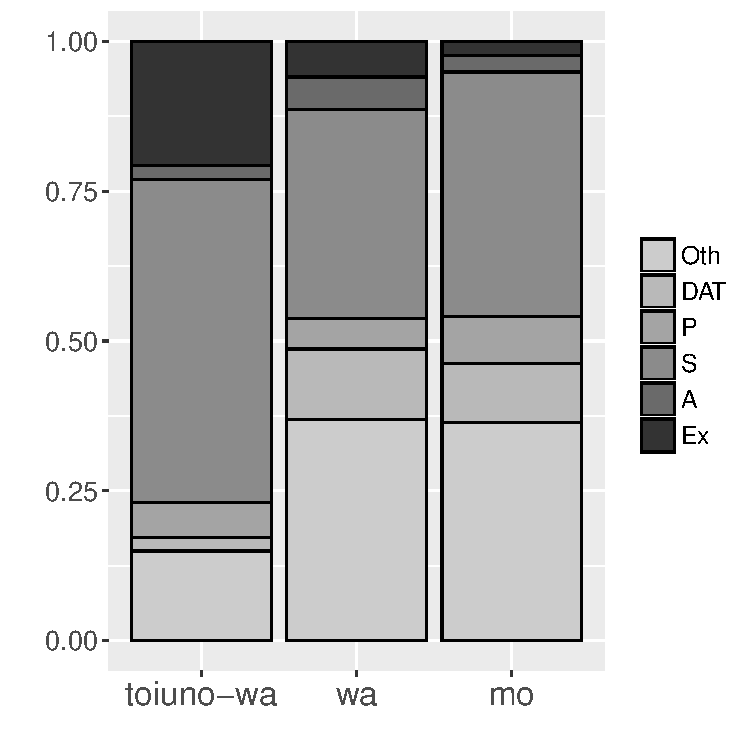
\includegraphics[width=0.5\textwidth]{figure/ASPTopPar.pdf}
	\caption{Topic markers vs.~grammatical function}
	\label{Par:ASPTopParF}
	\end{center}
%\end{minipage}
\end{figure}
\begin{figure}
%\begin{minipage}{0.5\textwidth}
	\begin{center}
	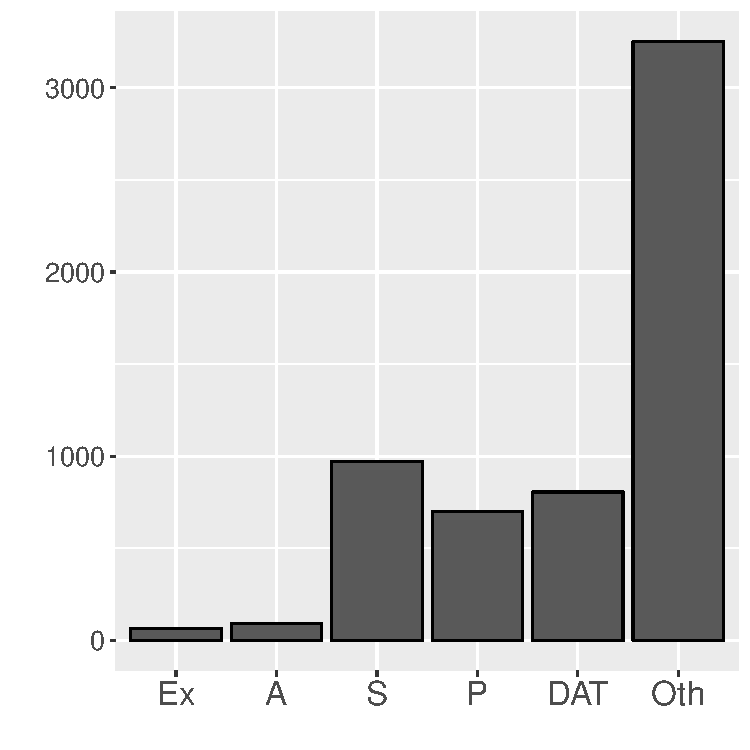
\includegraphics[width=0.5\textwidth]{figure/ASPall.pdf}
	\caption{Overall distributions of elements}
	\label{Par:ASPallF}
	\end{center}
%\end{minipage}
\end{figure}


Whereas \citeA[2]{aoki92} reported that
84.7\% of \ci{wa} attaching nouns code so-called subjects (A and S in my term, nominative case in her term) in novels and essays,
only 40.3\% of \ci{wa} in our data codes As and Ss
as shown in Table \ref{Par:ASPTopParT} and Figure \ref{Par:ASPTopParF}.
These table and figure include all kinds of elements excluded in other analyses.%
 \footnote{
 Refer to \S \ref{FW:Cor:AnaRel} to see what is excluded.
 }
Figure \ref{Par:ASPallF},
which represents the overall frequencies of elements,
is shown for comparison.
This graph also includes all kinds of elements excluded in other graphs.
On the other hand, Table \ref{Par:ASPTopParT} and Figure \ref{Par:ASPTopParF} show that
59.0\% of \ci{toiuno-wa} codes so-called subjects.
This demonstrates that
\ci{toiuno-wa} in spoken Japanese is in fact closer to \ci{wa} in written Japanese
in terms of the preference of coding grammatical functions. %and the functions of spoken \ci{wa} are shifting.
Although a majority of the literature focuses on \ci{wa} coding subjects,
the results suggest that \ci{wa} codes other kinds of elements in spoken Japanese.

So-called subjects have some special status in the discourse;
they are interpreted to be definite in the discourse
even though the NP is coded by \ci{ga} instead of \ci{wa}.
For example,
consider the difference between \Next and \NNext.
%
\ex.
 \a.[Q:] Why were you absent yesterday?
 \bg.[A:] \EM{kuruma-ga} inu-o hii-ta-n-desu \\
		car-\ci{ga} dog-\ci{o} run.over-\ab{past}-\ab{nmlz}-\ab{plt} \\
		`(My) car ran over (a) dog.'
 \bg.[A$^{\prime}$] \EM{kuruma-ga} inu-ni butukat-ta-n-desu \\
   car-\ci{ga} dog-\ab{dat} hit-\ab{past}-\ab{nmlz}-\ab{plt} \\
   `(My) car hit (a) dog.'
%			\b. My dog ate a toy.
%			\b. A toy was eaten by my dog.
	
\ex. \a.[Q:] Why were you absent yesterday?
	\bg.[A:] \EM{inu-ga} kuruma-ni hik-are-ta-n-desu \\
		dog-\ci{ga} car-\ab{dat} run.over-\ab{pass}-\ab{past}-\ab{nmlz}-\ab{plt} \\
		`(My) dog was run over by (a) car.'
 \bg.[A$^{\prime}$] \EM{inu-ga} kuruma-ni butukat-ta-n-desu \\
   dog-\ci{ga} car-\ab{dat} hit-\ab{past}-\ab{nmlz}-\ab{plt} \\
   `(My) dog hit (a) car.'
%			\b. A dog ate my toy.
%			\b. My toy was eaten by a dog.

These utterances represent the same propositional meaning
that can be something like `(a/the) car ran over (a/the) dog.'
Note that,
since Japanese does not have obvious ways to code definiteness,
both `car' and `dog' can be potentially interpreted as either definite or indefinite,
and hence `car' and `dog' are expressed in the same way in \LLast and \Last
except for case markers.
Under these conditions,
the subjects `car' in \LLast and `dog' in \Last are interpreted as definite, % and are associated with the speaker,
while the non-subjects `car' in \Last and `dog' in \LLast are indefinite,
according to the author's intuition.
NPs coded by \ci{wa} are also likely to be interpreted as definite since
the referent of those NPs are assumed to be evoked.
This observation suggests that subjects without topic-marking still function like topic markers.
This is worth investigating in the future
since my argument is no more than an impressionistic analysis.


%Similarly,
%the contrast between \Next[-A2] and \Next[-A2$^{\prime}$] and  shows that
%the subject `friend' in \Next[-A2] can only be interpreted as the speaker's friend
%(if there are no other salient people in the context),
%while the object `friend' in \Next[-A2$^{\prime}$] can be interpreted as the speaker's friend or the subject Taro's friend.
%%
%\ex.
% \a.[A1:] Oh my gosh...
% \b.[B1:] What happened?
% \bg.[A2:] ima \EM{tomodati-ga} taroo nagut-ta-n-da-yo \\
%   now friend-\ci{ga} Taro hit-\ab{past}-\ab{nmlz}-\ab{cop}-\ab{fp} \\
%   `(My) friend hit Taro just now.'
% \bg.[A2$^{\prime}$:] ima \EM{taroo-ga} tomodati nagut-ta-n-da-yo \\
%   now Taro-\ci{ga} friend hit-\ab{past}-\ab{nmlz}-\ab{cop}-\ab{fp} \\
%   `Taro hit (my/his) friend just now.'
%

%%% Silversteinの名詞句階層と角田

%%----------------------------------------------------
\subsection{Hierarchy of topic-coding}\label{Par:ArgStr:TopHierarchy}

There seems to be a hierarchy of topic-coding;
given As and Ss are more likely to be coded by topic markers than given Ps.
For example, consider the following example.
In \Next,
\ci{sohu} `grandfather' is introduced in line a, and
\ci{pan} `bread' is introduced in line b.
In line c, which is of interest in the discussion,
\ci{oziityan} `grandfather' is coded by \ci{wa}, but
\ci{sore} `that' referring to the bread in line b is coded by the case particle \ci{o}.
%
\ex.
 \ag. uti-no \EM{sohu}-tteiuno-ga okasi-ga sukina mono-de \\
 		out-\ab{gen} grandfather-\ci{toiuno}-\ci{ga} sweet-\ci{ga} favorite thing-\ab{cop} \\
		`Our grandfather likes sweets.'
 \bg. yoku pan-ya-san-de \EMi{kasi-pan}-o kat-te kuru-n-desu-ga \\
   often bread-store-\ab{hon}-\ab{loc} sweet-bread-\ci{o} buy-and come-\ab{nmlz}-\ab{cop}.\ab{plt}-though \\
   `(He) often buys sweet bread and comes home,'
 \bg. e n \EMi{sore-o} i maa yoowa \EM{oziityan-wa} issyookenmee taberu-n-desu-keredomo \\
   \ab{fl} \ab{frg} that-\ci{o} \ab{frg} \ab{fl} in.a.word grandfather-\ci{wa} trying.best eat-\ab{nmlz}-\ab{cop}.\ab{plt}-though \\
   `that, he tries his best to eat it, but'
 \b. he cannot eat all and
 \b. gives leftovers to the dog...
  \hfill{(\code{S02M0198: 244.48-262.82})}

It is unnatural for \ci{wa} to code \ci{sore} referring to the bread
instead of \ci{oziityan} `grandfather',
as shown in \Next[c$^{\prime}$].
If A (e.g., \ci{obaatyan} `grandmother') is newly introduced as in \Next[c$^{\prime\prime}$],
there is no problem for \ci{wa} coding \ci{sore};
\ci{obaatyan} `grandmother' is naturally coded by \ci{ga} instead of \ci{wa}.
%
\ex.
 \ag.[c$^{\prime}$.] e n \EMi{sore-\{o/wa\}} i maa yoowa ??\EM{oziityan-ga} issyookenmee taberu-n-desu-keredomo \\
   \ab{fl} \ab{frg} that-\{\ci{o}/\ci{wa}\} \ab{frg} \ab{fl} in.a.word grandfather-\ci{ga} trying.best eat-\ab{nmlz}-\ab{cop}.\ab{plt}-though \\
   `that, my grandfather tries his best to eat it, but...'
  \bg.[c$^{\prime\prime}$.] e n \EMi{sore-\{o/wa\}} i maa yoowa \EM{obaatyan-\{ga/??wa\}} issyookenmee taberu-n-desu-keredomo \\
   \ab{fl} \ab{frg} that-\{\ci{o}/\ci{wa}\} \ab{frg} \ab{fl} in.a.word grandmother-\ci{ga}/\ci{wa} trying.best eat-\ab{nmlz}-\ab{cop}.\ab{plt}-though \\
   `that, my grandmother tries her best to eat it, but...'
   \hfill{(modified from \Last[c])}

In fact, the majority of anaphoric Ps are still coded by \ci{o},
instead of topic markers,
whereas more ratio of anaphoric As and Ss are coded by topic markers.
Table \ref{Par:ASPParGivenT} and \ref{Par:ASPParNewT} and
Figure \ref{Par:ASPParGivenF} and \ref{Par:ASPParNewF} show
the distributions of topic and case markers coding A, S, and P.
Table \ref{Par:ASPParGivenT} and Figure \ref{Par:ASPParGivenF} represent the distributions of topic and case markers coding anaphoric A, S, and P.
As the table and the graph show,
while 44.1\% of anaphoric As and 38.8\% of anaphoric Ss are coded by topic markers,
only 8.4\% of anaphoric Ps are coded by topic markers.
On the other hand,
the majority of non-anaphoric elements are coded by case markers,
although non-anaphoric Ss (most of which are in fact inferable) are remarkably more coded by \ci{wa} than others.

I propose the hierarchy \Next for topic-coding.
The given elements higher in this hierarchy are more likely to be coded by topic markers.
%
\ex.\label{ASPGivenSchema}
 A, S $>$ P

The hierarchy indicates that so-called subjects are more likely to be coded by topic markers.
This hierarchy is a topic hierarchy:
the hierarchy of elements which are more likely to be topics \cite{givon76,keenan76,comrie79,comrie83,dubois87}.
%%% あやしい
This hierarchy is present in many languages in various ways.
For example, A and S are more likely to be agreed with the verb than P cross-linguistically.
Also, A and S are more likely to be zero-coded than P.
Japanese \ci{wa}-coding seems to follow this hierarchy;
if there are two given elements potentially coded by \ci{wa},
A and S are preferred over P following the hierarchy \Last.

\begin{table}
\begin{center}
\tblcaption{Markers for anaphoric}
\label{Par:ASPParGivenT}
\begin{tabular}{lrrrr}
	\toprule
	              & Ex & A & S & P \\
	\midrule
	 Topic marker & 20 & 15 & 97 & 15 \\
	              & \rt{(100\%)} & \rt{(44.1\%)} & \rt{(38.8\%)} & \rt{(8.4\%)} \\
	 Case marker  & 0 & 19 & 153 & 163 \\
	              & \rt{(0\%)} & \rt{(55.9\%)} & \rt{(61.2\%)} & \rt{(91.6\%)} \\
	\midrule
	 Sum          & 20 & 34 & 250 & 178 \\
	              & \rt{(100\%)} & \rt{(100\%)} & \rt{(100\%)} & \rt{(100\%)} \\
	\bottomrule
%             Ex   A   S   P DAT
%  toiuno-wa   9   1  26   2   0
%  wa          11  14  71  13   0
%  ga          0  19 153   0   0
%  o           0   0   0 163   0
\end{tabular}
\end{center}
\end{table}

\begin{table}{}
\begin{center}
\tblcaption{Markers for non-anaphoric}
\label{Par:ASPParNewT}
\begin{tabular}{rrrr}
	\toprule
	 Ex & A & S & P \\
	\midrule
	 12 & 1 & 74 & 13 \\
	 \rt{(100\%)} & \rt{(8.3\%)} & \rt{(21.6\%)} & \rt{(6.8\%)} \\
	 0 & 11 & 269 & 177 \\
	 \rt{(0\%)} & \rt{(91.7\%)} & \rt{(78.4\%)} & \rt{(93.2\%)} \\
	\midrule
	 12 & 12 & 343 & 190 \\
	 \rt{(100\%)} & \rt{(100\%)} & \rt{(100\%)} & \rt{(100\%)} \\
	\bottomrule
%             Ex   A   S   P DAT
%  toiuno-wa   8   1  16   3   0
%  wa          4   0  58  10   0
%  ga          0  11 269   0   0
%  o           0   0   0 177   0
\end{tabular}
\end{center}
\end{table}

\begin{figure}
%\begin{minipage}{0.5\textwidth}
	\begin{center}
	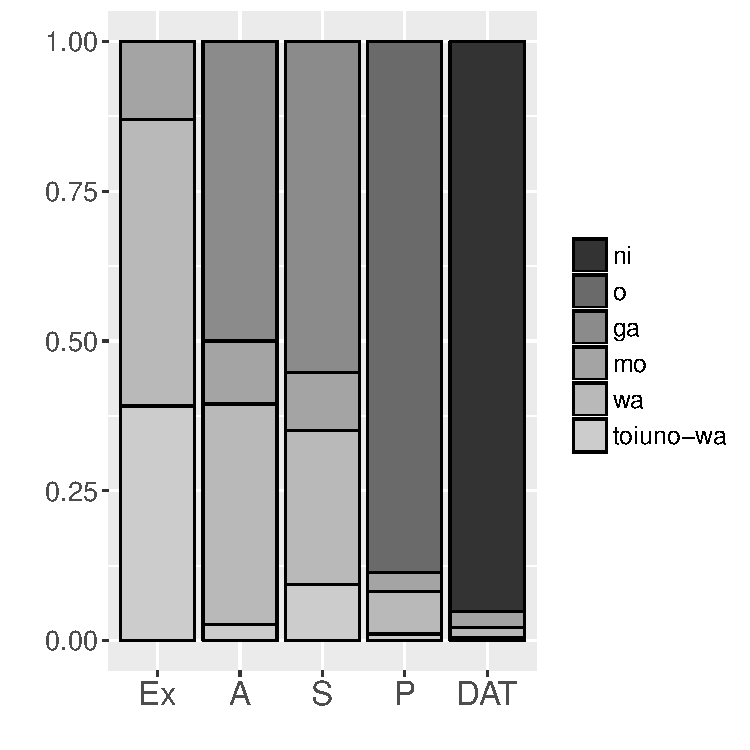
\includegraphics[width=0.5\textwidth]{figure/ASPParGiven.pdf}
	\caption{Markers for anaphoric}
	\label{Par:ASPParGivenF}
	\end{center}
\end{figure}
\begin{figure}
%\end{minipage}
%\begin{minipage}{0.5\textwidth}
	\begin{center}
	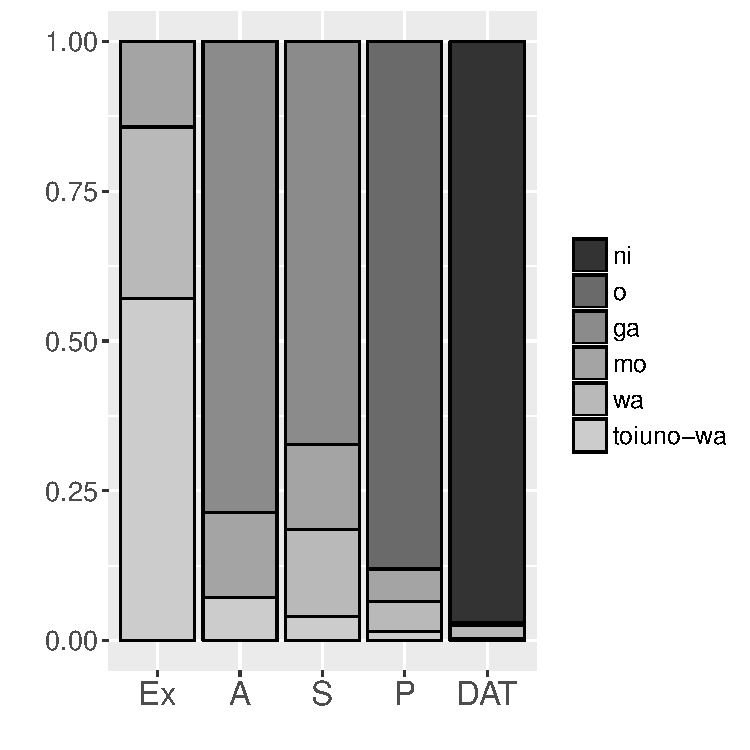
\includegraphics[width=0.5\textwidth]{figure/ASPParNew.pdf}
	\caption{Markers for non-anaphoric}
	\label{Par:ASPParNewF}
	\end{center}
%\end{minipage}
\end{figure}


%%----------------------------------------------------
\subsection{Ex or detached NPs}\label{Par:Subj:Ex}

Finally, I discuss associations between ``Ex'' and topic markers.
In \S \ref{FW:Cor:TopFoc},
Ex was defined as elements ``which appear to be part of the clause but do not have direct relationships with the predicate'' (p.~\pageref{FW:Cor:TopFoc:ExDef}).
A typical example is shown in \Next.
In \Next, the predicate \ci{nagai} `long' is directly related to \ci{hana} `nose'.
\ci{Zoo} `elephant' is not directly related to the predicate;
it is not the elephant itself that is long.
%
\exg. \EM{zoo-wa} hana-ga nagai \\
		elephant-\ci{wa} nose-\ci{ga} long \\
		`The elephant, the nose is long (The elephant has a long nose).' \hfill{\cite{mikami60}}

Table \ref{Par:ASPParGivenT} and \ref{Par:ASPParNewT} and
Figure \ref{Par:ASPParGivenF} and \ref{Par:ASPParNewF}
show that Ex is only coded by topic markers.
Table \ref{Par:ASPTopParT} and Figure \ref{Par:ASPTopParF}
show that 21.7\% of \ci{toiuno-wa}-coded elements and
5.9\% of \ci{wa}-coded elements are categorized into Ex.

\citeA{lambrecht94}
discusses cross-linguistic cases of Ex (in his term, ``detached'' topic)
and argues that
``in some languages at least, the detached topic NP cannot be a constituent [...] of the clause with which it is pragmatically associated'' (p.~192).
In \Next, examples in English,
the detached topics are not constituents of the clause;
rather, they have a part-whole relation with some element(s) within a clause.
In \Next[a], the detached topic \ci{the typical family today} is not a constituent of the clause;
instead, it is associated with \ci{the husband and the wife} pragmatically.
In the same way, the detached topics \ci{tulips} in \Next[b] and
\ci{other languages} in \Next[c]
are pragmatically associated with constituents of the clauses \ci{bulbs} and \ci{tones}, respectively.
%
\ex.
% \a. (Six year old girl, explaining why the African elephant has bigger ears than Asian elephant) \\
%  \EM{The African elephant}, it's so hot there, so \EM{he} can fan himself.
 \a. (From a TV interview about the availability of child care) \\
   That isn't the typical family anymore.
   \EM{The typical family today},
   \EMt{the husband and the wife} both work.
 \b. (Talking about how to grow flowers) \\
   \EM{Tulips}, you have to plant new \EMt{bulbs} every year?
 \b. (Lecture in an introductory linguistics course) \\
   \EM{Other languages}, you don't just have straight \EMt{tones} like that.
% \b. (From an article in the San Fransisco Chronicle about a wealthy town in Dade Country, Florida, becoming a ``'fort against crime') \\
%   ``what we are trying to do here is keep this community what it is, a beautiful, safe place to live,'' said police chief Dick de Stefani.
%   ``\EM{Dade Country}, you just can't belive the rise in crime.''
  \b.[] \hfill{\cite[193]{lambrecht94}}

These detached topics are strikingly similar to
``Ex'' in Japanese.

Lambrecht also discusses cases in which
topics are not counted as constituent of the clause
even though they appear to be constituents.
German, for example, has the principle that only allows the verb in the second position within a clause as exemplified in \Next[a-d].
However, the detached topic constituents that appear at the beginning are not counted as the first constituent of the clause.
%rather they are outside of the clause.
As exemplified in \Next[e],
the verb \ci{isst} `ate' appears in the second position assuming that the preceding \ci{den} `it' is in the first position,
which indicates that
the detached topic \ci{den Apfel} is not counted as the first constituent in the clause.
In fact, as in \Next[f],
it is unacceptable
if the detached topic \ci{den Apfel} is counted as the first constituent.%
 \footnote{
 \chd{\ci{Apfel} `apple' in e, f of \ref{Par:Subj:Ex:Ex:Apfel} is considered to be ``detached'' because
 the resumptive pronoun \ci{den} `it.\ab{acc}' is regarded as argument of the clause and \ci{Apfel} itself does not function as argument.}
 }
%
\ex.\label{Par:Subj:Ex:Ex:Apfel}
 \ag. Hans \EM{isst} den Apfel. \\
   Hans eat the.\ab{acc} apple \\
   `Hans eats the apple.' \hfill{(SVO)}
 \b. Den Apfel \EM{isst} Hans. \hfill{(OVS)}
 \b. *Den Apfel Hans \EM{isst}.\hfill{(*OSV)}
 \bg. Den isst Hans. \\
   it.\ab{acc} eat Hans \\
   `Hans eats it.' \hfill{(OVS)}
 \bg. \EMi{Den} \EMi{Apfel} den \EM{isst} Hans. \\
   the.\ab{acc} apple it.\ab{acc} eat Hans \\
   `The apple, Hans eats it.'  \hfill{(TOVS)}
 \b. *\EMi{Den} \EMi{Apfel} \EM{isst} Hans den. \hfill{(*TVSO)}
 \b.[] \hfill{(op.cit.: p.~194)}

Both the topicalized NP \ci{den Apfel} and the resumptive pronoun \ci{den} in \Last[e] appear as accusative.
According to Lambrecht, however,
it is optional for the topicalized NP,
while it is obligatory for the resumptive pronoun.
This is also reminiscent of topic-marking in Japanese.
In Japanese,
nominative and accusative codings are overridden by topic-marking
and the case for A, S, and P coded by topic markers are not overtly expressed
as has been discussed in \S \ref{Back:GeneralChar:Wa}.
%Whereas the detached topic \ci{den Apfel} in the examples above have the coreferent pronoun \ci{den} within the clause,
%He discusses cases where the detached topics do not have the coreferent in the clause:
%examples of unlinked topic construction.


The fact that topics tend to be ``detached'' from the predicate and
lose case marking cross-linguistically suggests the possibility that
there are some universal motivations behind this phenomenon.
I argue that at least one of the motivations is clause-chaining.
In clause-chaining,
the speaker combines multiple clauses to form a thematic unit
\cite{longacre85,martin92,givon01}.
\Next is an example of clause-chaining.
%
\ex. She came in, [\O] stopped, [\O] looked around and froze.\\
     \hfill{\cite[349]{givon01}}

By combining clauses in this way,
thematic continuity is achieved.
In clause-chaining,
the detached topic, which typically appears utterance-initially as will be discussed in Chapter \ref{WordOrder},
is not necessarily an argument of the clauses;
instead, it is pragmatically related to the following clauses.
For example, in \Next,
where the speaker talks about a life in Iran,
\ci{mukoo-no hito} `people there (in Iran)' in \Next[a] is detached
and annotated as ``Ex''
because its predicate \ci{hukaku} `deep', which has a part-whole relations with the people, has the so-called subject \ci{hori} `(face) form'.
In \Next[b-c], the speaker continues to talk about Iran people
by clause-chaining.
\ci{Kodomo} `child' in \Next[c] also has a part-whole relation
with the Iran people.
%
\ex.
 \ag. eto n \EM{mukoo-no} \EM{hito-toiuno-wa} hontooni \EMi{hori-ga} hukaku-te \\
      \ab{fl} \ab{fl} there-\ab{gen} person-\ci{toiuno-wa} really form-\ci{ga} deep-and \\
      `People there (in Iran), (their) face forms are really chiseled,'
 \bg. kiree-de \\
      beautiful-and \\
      `beautiful,'
 \bg. \EMi{kodomo-nanka-wa} anoo sugoku kawaii kao-o si-tei-mashi-ta \\
      child-\ab{hdg}-\ci{wa} \ab{fl} very cute face-\ci{o} do-\ab{prog}-\ab{plt}-\ab{past} \\
      `children had very cute faces.'
      \src{S03F0072: 375.01-386.35}
%S03F0072|00375010L|375.010443|386.346614|L|(F えと)(D ん)(0.507)向こうの人というのは本当に(F あのー)彫りが深くて(0.229)奇麗で(0.907)(F えーと)子供なんかは(0.587)(F あのー)凄く(1.012)かわいい顔をして(0.627)いました|[文末]|

Clause-chaining is a useful way to talk about something;
the speaker puts the topic at the beginning and
continue to describe the topic as much as s/he can.
In the descriptions in clause-chaining,
the topic is not necessarily an argument;
it is pragmatically associated with each clause.
The hearer does not get lost.
The hearer can trace the topic
when the speaker provides enough evidence
through linguistic expressions (such as particles, word order, and intonation) and other means (such as gesture, background knowledge, sequence of conversation, etc.).

\citeA[Chapter 2]{mikami60} points out that
\ci{wa}-coded NPs can ``go beyond periods'' (p.~117) and ``commas'' (p.~130).
This is closely related to what I argue here.
%
%\ex.
% \ag. \EM{tookyoo-wa} kinbenna hito-ga takusan i-te \\
% \bg. issyookenmee hatarai-teiru-no-da-ga \\
% \bg. mati-mo kitanai-si \\
% \bg. miti-mo kitanai \\
%
He states:
``in general, `X-\ci{wa}', skipping adverbial clauses in the middle, governs the final main clause.
However, it [sometimes] governs the verbs in the middle a little bit;
this is what I call [\ci{wa}'s] going beyond commas'' (p.~130).
Of course, there are no commas and periods in spoken language,
\ci{wa} and \ci{toiuno-wa} go beyond ``commas'' and ``periods'' by governing the whole clause-chaining.
%In \S \ref{Back:GeneralChar:Wa},

%%----------------------------------------------------
%%----------------------------------------------------
\section{Discussion}\label{ParticlesDiscussion}

%%----------------------------------------------------
\subsection{Distribution of markers and semantic space}

\begin{figure}
%\begin{minipage}{0.5\textwidth}
	\begin{center}
	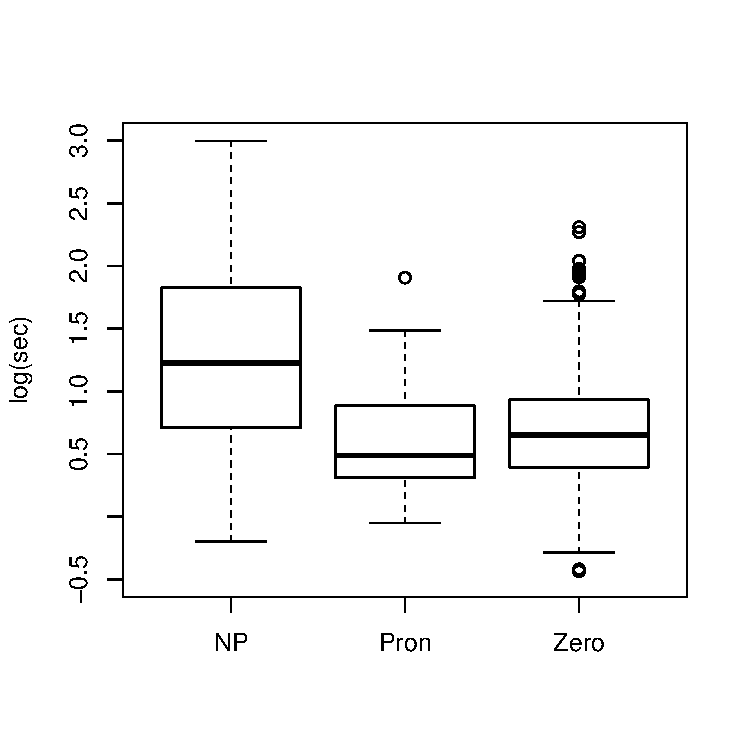
\includegraphics[width=0.5\textwidth]{figure/DistExpType.pdf}
	\caption{Anaphoric distance vs.\ expression type (all)}
	\label{DistExpTypeF2}
	\end{center}
%\end{minipage}
%\begin{minipage}{0.5\textwidth}
%	\begin{center}
%	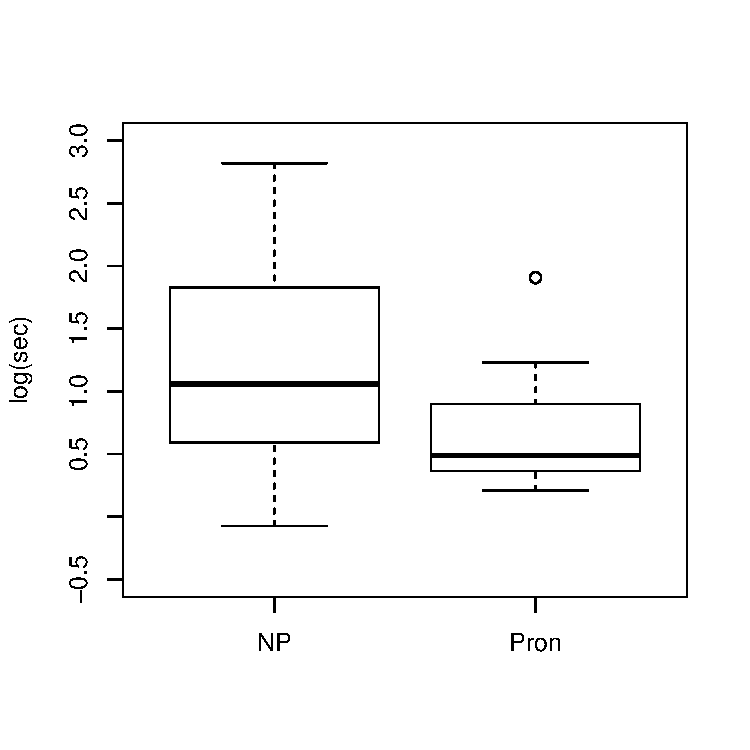
\includegraphics[width=0.99\textwidth]{figure/DistExpTypeTop.pdf}
%	\caption{Anaphoric distance vs.\ expression type (coded by topic markers)}
%	\label{DistExpTypeParF}
%	\end{center}
%\end{minipage}
\end{figure}

As discussed in \S \ref{ParIntro},
the particles code elements with features that can be mapped onto a conceptual space.
As in Table \ref{ParInfoStatusT} and discussion in \S \ref{TopPar},
topic markers map onto a conceptual space of given-new taxonomy,
while, as in Table \ref{OvertZeroCaseParT1} and discussion in \S \ref{CasePar},
case markers map onto a conceptual space of agentivity, focushood, contrastiveness, and possibly animacy.

The semantic map of topic markers in Japanese indicates that
inferable and evoked statuses form a connected region and are expressed by the same marker \ci{wa},
while declining and unused statuses form a connected region and are expressed by the same marker a copula followed by \ci{kedo} or \ci{ga};
hence, the inferable status is closer to the evoked status, and the declining status is closer to unused in the conceptual space.
This makes sense because inferable elements are more relevant to
the current topic than declining elements.
For example, in \Next,
the inferable element \ci{gen'in} `cause' is coded by \ci{wa}.
The element `cause' is inferable because the disease has been already introduced and the cause of the disease can be considered to be part of the knowledge of getting a disease.
%
\ex.
 \a. (The speaker got a wired disease.)
 \b. First I visited several local hospitals.
 \b. I was examined several times, but
 \bg. \EM{gen'in-wa} humee-de \\
   cause-\ci{wa} unclear-\ab{cop} \\
   `the cause (of the disease) was unclear.'
   \hfill{(\code{S02F0010: 74.93-82.60})}
%
%まず地元の病院のを何軒か回りました
%でその度に検査をして
%あの調べたんですが
%原因は不明で (S02F0010: 74.93-82.60)

In \Last,
the cause of the disease is relevant to the current topic, i.e., the speaker's disease.
Later in this speech,
the speaker talks about her parents and friends;
in this case the cause of the disease is considered to be declining and is less relevant to the current topic (her parents and friends).
Declining elements like the cause of the disease become unused as the time passes.
If the speaker brings up the cause of the disease two days later,
she will code it as unused.
Thus, I argue that the adjacency of inferable and evoked statuses and that of declining and unused statuses are cognitively motivated and I argue that this is universal.

Moreover,
I propose that there are at least two kinds of evoked status:
evoked and what I call strongly evoked.
Evoked elements are full NPs, and
strongly evoked elements are zero and overt pronouns.
%Active elements are, as I have discussed so far,
%coded by \ci{toiuno-wa} and \ci{wa}.
%Strongly active elements are, on the other hand, so-called zero pronouns.
%Zero pronouns are more active than elements coded by \ci{toiuno-wa} and \ci{wa}.
Figure \ref{DistExpTypeF2} shows the time difference (anaphoric distance) on logarithmic scale between the first mora of the element in question is produced and that of its antecedent is produced.
Zero pronouns are assumed to be produced at the time when
the first mora of the predicate is produced.
The anaphoric distance approximates activation cost;
smaller distance indicates lower activation cost,
while larger distance indicates higher activation cost.
Figure \ref{DistExpTypeF2} represents the anaphoric distance of three kinds of elements:
full NPs, pronouns, and zero pronouns.
%Figure \ref{DistExpTypeParF} indicates the distance of elements coded by \ci{toiuno-wa} and \ci{wa}.
As is clear from the figure,
the anaphoric distance of zero and overt pronouns is smaller than
that of NPs,
which indicate that
zero and overt pronouns are more evoked than full NPs \chd{(fixed effects model, $p < 0.001$)}.
Therefore, I propose the status called ``strongly evoked''.
I add this status in Table \ref{ParInfoStatusT2}.
Since overt pronouns coded by topic markers are as strongly evoked as zero pronouns,
I suppose that topic markers \ci{wa} and \ci{toiuno-wa} can also code strongly evoked elements.
%%% Strongly activeだったら、トイウノハとハも付ける

Markers for focus coding map onto agentivity, focushood, contrastiveness, and possibly animacy
as has been discussed in \S \ref{CasePar}.
Table \ref{OvertZeroCaseParT} in \S \ref{CasePar} indicates that
A and agent S are adjacent to each other, and
patient S and P are adjacent.
This makes sense because
A is conceptually closer to agent S, and
P is conceptually closer to patient P.
%I will discuss other features such as focushood and animacy in the following section.

\begin{table}[hbt]
	\caption{Topic marker vs.\ activation status and given-new taxonomy}
	\label{ParInfoStatusT2}
	\begin{center}
	\begin{tabular}{|l|l|c|c|}
	\hhline{----}
	Activation status & Given-new taxonomy & Topic & Focus \\
	\hhline{|-|-|-|-|}
	                 &        & Zero pronoun  & -- \\
	\hhline{|~|~|~|-|}
	 Strongly active & Evoked & Overt pronoun &  \\
	                 &        & \ci{toiuno-wa, wa}, {\O} &  \\
	\hhline{|-|-|-|~|}
	 Active & Evoked & \ci{toiuno-wa, wa}, {\O} &  \\
	\hhline{|-|-|-|~|}
	\cellcolor[gray]{.9}Semi-active & \cellcolor[gray]{.9}Inferable & \ci{wa}, {\O} & case markers, {\O} \\
	\hhline{|-|-|-|~|}
	 Semi-active & Declining & \multirow{2}{*}{\ab{cop}-\ci{kedo/ga}, {\O}}  &  \\
	\hhline{|-|-|~|~|}
	\cellcolor[gray]{.9}Inactive & \cellcolor[gray]{.9}Unused &  &  \\
	\hhline{|-|-|-|~|}
	\cellcolor[gray]{.9}Inactive & \cellcolor[gray]{.9}Brand-new &  --  &  \\
%	\rowcolor{gray}
%	 & (Anchored) & & \\
%	\rowcolor{gray}
%	inactive & Brand-new &  --  & case markers, {\O} \\
%	\rowcolor{gray}
%	 & (Unanchored) & & \\
	\hhline{----}
	\end{tabular}\\
	\end{center}
\end{table}

%%----------------------------------------------------
\subsection{Distribution of markers and markedness}\label{Par:Dis:Markedness}

As discussed in \S \ref{CasePar} and summarized in Table \ref{OvertZeroCaseParT},
the distinction between overt vs.\ zero particles for focus coding is sensitive to grammatical functions, contrastiveness, and animacy.
%while that for topic coding is sensitive to activation status and contrastiveness as discussed in \S \ref{TopPar}.
The distribution of overt vs.\ zero particles for non-contrastive focus coding in Table \ref{OvertZeroCaseParT}
is similar to that of split intransitive languages,
if one ignores \ci{ga}-coding for patient S.
In general, split intransitive languages code S differently
depending on whether it is an agent or a patient;
agent S is coded in the same way as A in the transitive clause,
while patient S is coded in the same way as P.
\Next shows examples from Georgian.%
	\footnote{
	Examples are from the handouts in the lecture called Typology and Universals given by Matthew Dryer at the University at Buffalo in 2010.
	Glosses are modified.
	}
\ex. Georgian, South Caucasian
	\ag. \tp{vano-\EMi{m}} \tp{gamozarda} \tp{Zma-\EMi{\O}} \\
		Vano-\ab{a} \ab{3}.\ab{3}.grow brother-\ab{p} \\
		`Vano raised his brother.' \hfill{(A \& P)}
	\bg. \tp{vano-\EMi{m}} \tp{imGera} \\
		Vano-\ab{a} 3.sing \\
		`Vano sang.' \hfill{(Agent S)}
%	\bg. \tp{bav\v{s}v-ma} \tp{i{\.*t}ira} \\
%		child-\ab{act} 3.cry \\
%		`The child cried.' \hfill{(agent S)}
	\bg. \tp{rezo-\EMi{\O}} \tp{gamoizarda} \\
		Rezo-\ab{p} 3.grow \\
		`Rezo grew up.' \hfill{(Patient S)}
%
%\ex. Choctaw
%	\ag. \tp{alla-t} \tp{ofi} \tp{poshohli-tok} \\
%		child-\ab{nom} dog rub-\ab{past} \\
%		`The child patted the dog.' \hfill{(A \& P)}
%	\bg. \tp{hattak-a-t} \tp{oho:yo} ahpali-tok \\
%		man-\ab{det}-\ab{nom} woman kiss-\ab{past} \\
%		`The man kissed the woman.' \hfill{(A \& P)}
%	\bg. \tp{katos-a-t} \tp{\~{\i}pa-tok} \\
%		cat-\ab{det}-\ab{nom} eat-\ab{past} \\
%		`The cat ate.' \hfill{(agent S)}

Spoken Japanese and Georgian in \Last follow the typological tendency that
agent S and A tend to be overtly coded,
while patient S and P tend to be zero-coded.
%%% 文献
On the other hand,
Spoken Japanese does not follow the tendency of nominative/accusative languages:
the tendency that A and S (nominative elements) are more likely to be zero-coded than P (accusative elements).
I argue that, in coding focus elements,
patient elements are ``unmarked'',
i.e., more frequent than agent elements,
and are more likely to be zero-coded than agent elements.
This is supported in studies such as \citeA{dubois87} and \citeA{duboisetal03}.
On the other hand,
in coding topic elements,
agent elements are more frequent than patient elements,
and are more likely to be zero-coded than patient elements.
This is observed in another dialect of Japanese: Kansai Japanese.
In Kansai Japanese,
contrastive topic agents (A and agent S) can be zero-coded,
while contrastive topic patients (P and patient S) are overtly coded,
which is summarized in Table \ref{DistPartTopKJ}.
See \citeA{nakagawa13m}
for more detailed discussion on the relation
between markedness and the distribution of zero vs.\ overt particles in Standard and Kansai Japanese.

\begin{table}
\begin{center}
	\caption{Contrastive-topic coding in Kansai Japanese}
	\label{DistPartTopKJ}
\begin{tabular}{lcccc}
	\toprule
	 & A & \multicolumn{2}{c}{S} & P \\
\cline{3-4}
			 & & agent & patient & \\
	\midrule
%	inactive Topic & \cellcolor[gray]{.9} {\O} & \cellcolor[gray]{.9} {\O}  & \cellcolor[gray]{.9} {\O} & \cellcolor[gray]{.9} {\O} \\
%%	\rowcolor[gray]{0.95}
%	Activated Topic & \cellcolor[gray]{.9} {\O} & \cellcolor[gray]{.9} {\O}  &  \cellcolor[gray]{.9} {\O} & \cellcolor[gray]{.9} {\O} \\
%%	Activated Topic (SJ) & {\O}/\ci{wa} & {\O}/\ci{wa} & {\O}/\ci{wa} & {\O}/\ci{wa} \\
%%	\rowcolor[gray]{0.95}
	Contrastive Topic & {\O}/\ci{wa}  & {\O}/\ci{wa} & \ci{wa} & \ci{wa} \\
%	Contrastive Topic (SJ)  & \ci{wa} & \ci{wa} & \ci{wa} & \ci{wa} \\
	\bottomrule
\end{tabular}
\end{center}
\end{table}

As has been discussed in \S \ref{Par:CasePar:Ga:GaFoc},
\ci{ga} sometimes codes non-nominative focus NPs.
The theory of markedness also gives a hint to explain why \ci{ga} is on the way to grammaticalize into a focus particle;
focus A is the most rare in natural occurring discourse
and it is likely for Japanese native speakers to associate the marker \ci{ga} with focushood.
On the other hand, P is very frequently focus,
in which case, it is less likely to associate the marker \ci{o} with focushood.


%%%----------------------------------------------------
%\subsection{Continuity between topic and focus}\label{Par:Dis:Cont}


%%----------------------------------------------------
%%----------------------------------------------------
\section{Summary}

%%----------------------------------------------------
\subsection{Summary of this chapter}

This chapter discussed the distributions of so-called topic marker and case markers in Japanese.
I argued that
different markers are sensitive to different features, and
at the same time,
 multiple features contribute the usage of a single marker.


%%----------------------------------------------------
\subsection{Remaining issues}

While there are many remaining issues,
one of the biggest issues is that
it is necessary to test the proposals in this chapter through other empirical methods.
If the proposals are supported also by other methods,
they become more sound.
Especially the distribution of zero particles is mainly based on a few native speakers' acceptability judgements.
This should be tested with a larger number of native speakers.
One possible experiment is to ask subjects to listen to short conversation where the particles in question are blurred
and to produce what they hear.
This is easier than subtle acceptability judgements and linguistically na\"{\i}ve subjects can also participate in it.

Another issue is the focus test.
So far we only have the \ci{hee} test and the \ci{no} test,
which depend on the author's acceptability judgements.
One possible experiment is to ask subjects to listen to speech used in this study
and respond to what the speaker say by \ci{hee}
as if they were the hearers.
The elements that many subjects respond to are more likely to be foci.
Another possibility is to investigate conversations and study the elements that the hearer actually responds to.
\citeA{denetal12} annotated response tokens like \ci{hee} and the elements those response tokens address.
Thus it is not very difficult to seek the second possibility.


% !TEX root = ../main.tex
\chapter{Word Order}\label{WordOrder}

%%% ニガの語順を調べる
%%% Strongly active topicsは文頭に現れても良い

%%% 代名詞にアクセントがないことで、日本語の語頭アクセント規則(LH or HL)を破っている。よって後ろに現れるほうが良い。

%%% 前置された名詞はゼロになりやすいが、そうでない名詞はずっと繰り返し現れる。

%%% 文頭に現れる要素のすべてにトピック・マーカーがついているわけではない。トピック・マーカーはactivation statusに敏感だが、語順はidentityの方に敏感。

%%% Vallduv\UTF{00ED} (1994) のLink & Tailとの並行性を指摘。

%%% Gundel (1988)
%(52) Given before new principle
%     State what is given before what is new in relation to it.
%
%(53) First things first principle
%     Provide the most important information first.

%%% Rizziらのカートグラフィーに対する反論
%%% [TOPIC [FOCUS ...] ]
%%% 初期状態でこのような構造をしているという根拠はなく、トピックは文頭と文末、それぞれに現れる認知的動機付けが存在する

%%% フォーカスは動詞の直前 (Kuno, 1980)
%%% Tanaka (2005) 後置文の分析:選好応答は後置文

%%% 必ずしもDefiniteが文頭に来るわけではないというBackgroundのdefinitenessの節と矛盾

%%% 「へーテスト」にかける

%%----------------------------------------------------
%%----------------------------------------------------
\section{Introduction}\label{WO:Intro}

This chapter discusses how \isi{information structure} of a clause affects
\isi{word order}.

Figure \ref{DEPositionAllF} shows the overall distribution of elements
in terms of their positions in a clause.
%i.e.,
%elements' positions from the beginning of the clause in question
%to the last element of the current clause boundary.
Elements are counted by phrases (so called \ci{bunsetsu}).
The y-axis indicates the frequency of elements and
the x-axis indicates the position of elements:
\code{1} means that the element in question appeared in the first position in the clause,
\code{2} means that it appeared in the second position,
and so on.
I used the values of \code{nth} originally included in CSJ.
The reason why the frequencies of \code{1} and \code{2} are lower than \code{3} is that
the linguistic categories that appear in the first or second position
are typically fillers, connectives, and adjectives and
they are excluded from the analysis.
The fact that the elements later than fifth in the clause appear very frequently
might be counterintuitive based on the ordinary idea of a clause;
a clause consists of a single predicate and at most three arguments and a few more adjuncts.
In spoken language, however,
there are many fillers, intensifiers like \ci{hontooni} `really', and paraphrases,
which make the clause longer.
Since \code{nth} simply counts the position of a phrase in terms of linear position, and not structurally,
embedded clauses such as relative clauses are also included in the count.
\chd{I assume that it is worth including these intervening expressions
to analyze where a phrase can be interrupted by them and where it cannot.
In fact, the following results show that most non-\isi{anaphoric} elements appear immediately before the predicate, not interrupted by fillers, intensifiers, and so on (see \S \ref{WOPrePredEles}).}
Moreover,
CSJ has a unique definition of clause, which is not always the same as the intuitive of clause;
\chd{rather, a clause in CSJ is closer to a single series of clause-chaining.}
For example,
some subordinate markers such as \ci{-to} `if' and \ci{-te} `and' do not work as clause boundaries.
These characteristics cause more elements to appear in later positions.
See \citeA{maruyamaetal06} for a detailed definition of clause unit.

Figure \ref{DEPositionISF} and \ref{DEPositionPerF} show
element positions and their frequencies based on \isi{information status} and persistence, respectively.
The \isi{information status} ``\isi{anaphoric}'' in this study just means ``the element in question has a co-referential \isi{antecedent}'' and ``non-\isi{anaphoric}'' means ``it does not.''
``Persistent'' means ``the referent in question is also mentioned in the following \isi{discourse}'', and ``non-persistent'' means ``it is not.''%
%%%ISSUE "means" out of alignment.
See \S \ref{FW:Cor:AnaRel} for the detail of the annotation procedure.
\chd{As was discussed in \S \ref{TopPar},
a linear mixed effects model was employed to predict \isi{information status} (\isi{anaphoric} vs.~non-\isi{anaphoric}).
As fixed effects, \isi{word order} (\code{nth} in CSJ, see \S \ref{WO:Intro} for the definition of this annotation), particles (\ci{toiuno-wa, wa, mo, ga, o, ni}), and intonation (phrasal vs.~\isi{clausal} IU, see \S \ref{Int:PIUCIU} for the definitions) were included, and
as a random effect, the speaker (\code{TalkID}) was included.
The model with the effects of \isi{word order}, particles, and intonation is significantly different from the models without each of them, which indicates that
\isi{word order}, particles, and intonation respectively contribute to the prediction of \isi{information status}.
The model with all three effects is significantly different from the model without the effect of \isi{word order} (likelihood ratio test, $p < 0.01$);
it is significantly different from the model without the effect of particles ($p < 0.001$) and the model without the effect of intonation ($p<0.05$)}

\chd{As was also discussed in \S \ref{TopPar},
a linear mixed effects model was also applied to predict persistence (persistent vs.~non-persistent).
Word order, particles, and intonation were included as fixed effects, and
the speaker (\code{TalkID}) was included as a random effect.
The model with the effects of \isi{word order} and particles is again significantly different from the models without either of them (likelihood ratio test, $p < 0.01$ for the model without \isi{word order}, $p < 0.001$ for the model without particles).
However, the model with the effect of intonation is not significantly different from the model without it ($p=0.423$)}
The results are to be discussed more in \S \ref{WOSentInitEles}.

\begin{figure}
%\begin{minipage}{0.5\textwidth}
%	\begin{center}
	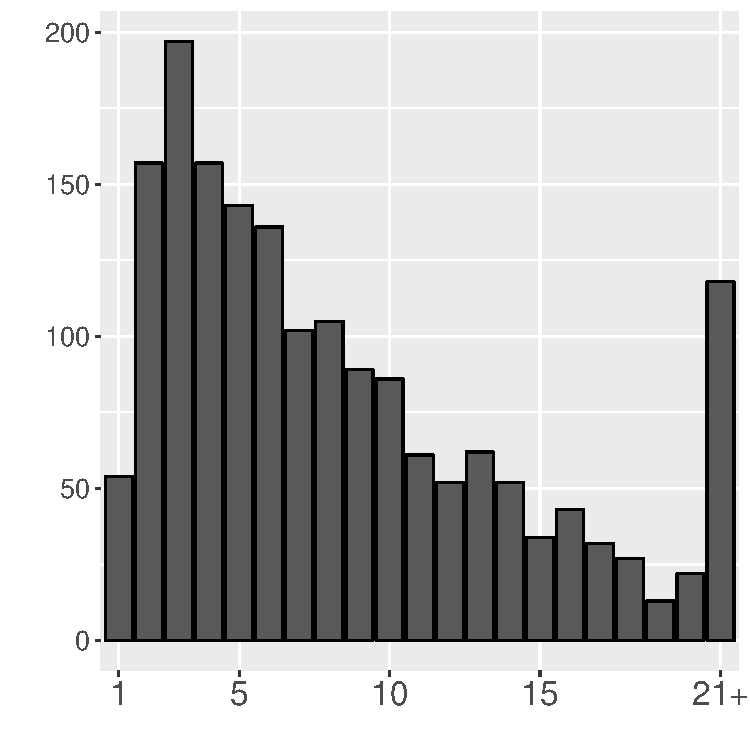
\includegraphics[width=0.7\textwidth]{figure/DEPositionAll.pdf}
	\caption{Order of all elements}
	\label{DEPositionAllF}
%	\end{center}
%\end{minipage}
\end{figure}
\begin{figure}
%\begin{minipage}{0.5\textwidth}
%	\begin{center}
	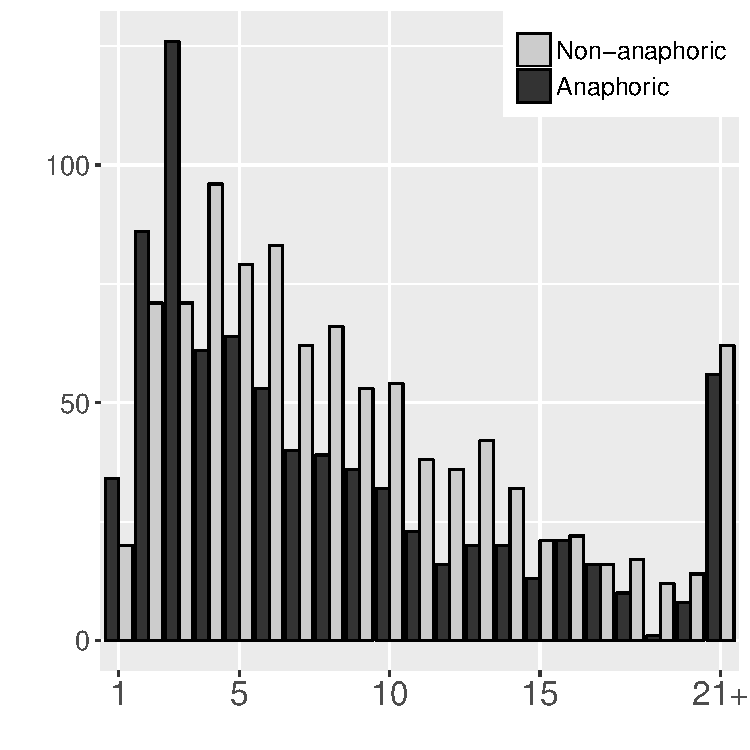
\includegraphics[width=0.7\textwidth]{figure/DEPositionIS.pdf}
	\caption{Word order vs.\ infoStatus}
	\label{DEPositionISF}
%	\end{center}
%\end{minipage}
\end{figure}
\begin{figure}
%\begin{minipage}{0.5\textwidth}
%	\begin{center}
	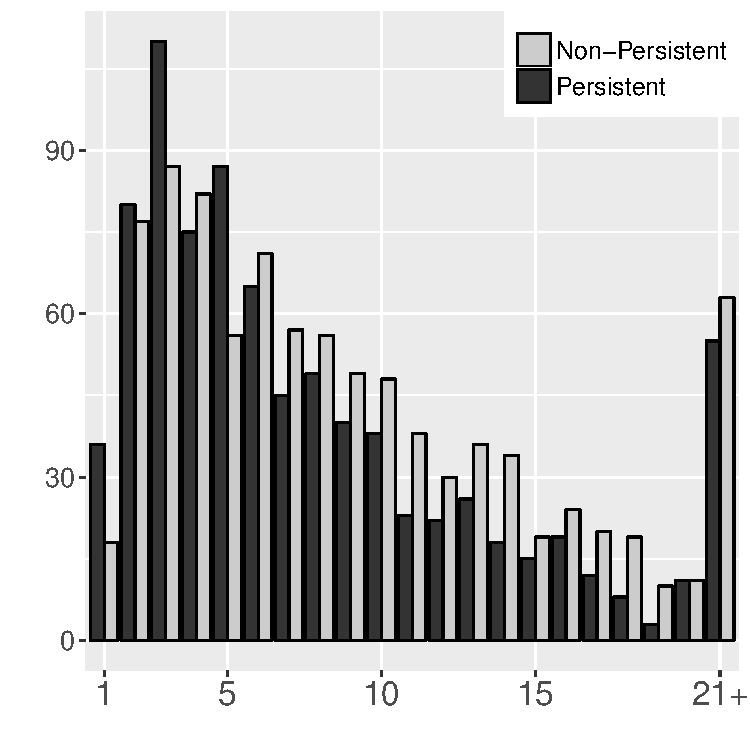
\includegraphics[width=0.7\textwidth]{figure/DEPositionPer.pdf}
	\caption{Word order vs.\ persistence}
	\label{DEPositionPerF}
%	\end{center}
%\end{minipage}
\end{figure}

%%%ISSUE Figures and texts are too far away because only one figure appears on one page. Also, some figures are too big.

Figure \ref{DiffAllF} shows the overall distribution of elements in terms of their distance from the predicate;
%\code{0} indicates that the element in question is the predicate itself,
\code{1} indicates that the element appears right before the predicate,
\code{2} indicates that there is one element between the preceding element and the following predicate, and so on.
If the element appears right after the predicate,
the distance is counted as \code{-1}.
Since the numbers of post-predicate elements are too small to achieve any generalization,
they are excluded from the figures.
Post-predicate elements will be discussed in comparison with dialogues
in \S \ref{WOPostPreEles}.

Figures \ref{DiffInfoStatusF} and \ref{DiffPerF} show the distance between the element and the predicate
depending on \isi{information status} and persistence.
\chd{A linear mixed effects model of \isi{information status} (the distance from the predicate and particles as fixed effects and the speaker as a random effect) indicates that
whereas the model with particles is significantly different from the model without them (likelihood ratio test, $p<0.001$),
the difference between the models with and without the distance from the predicate is only marginally significant ($p=0.060$).
This entails that the effect of particles significantly contributes to the model,
but the effect of the distance is inconclusive (see \S \ref{WOPrePredEles} for discussion).
On the other hand, a linear mixed effects model of persistence (fixed and random effects are the same as above) shows that the effects of both particles and the distance are significant to the model ($p<0.01$ for both the model without particle and that without the distance).}
The results are also to be discussed in further detail in \S \ref{WOPrePredEles}.


\begin{figure}
%\begin{minipage}{0.5\textwidth}
%	\begin{center}
	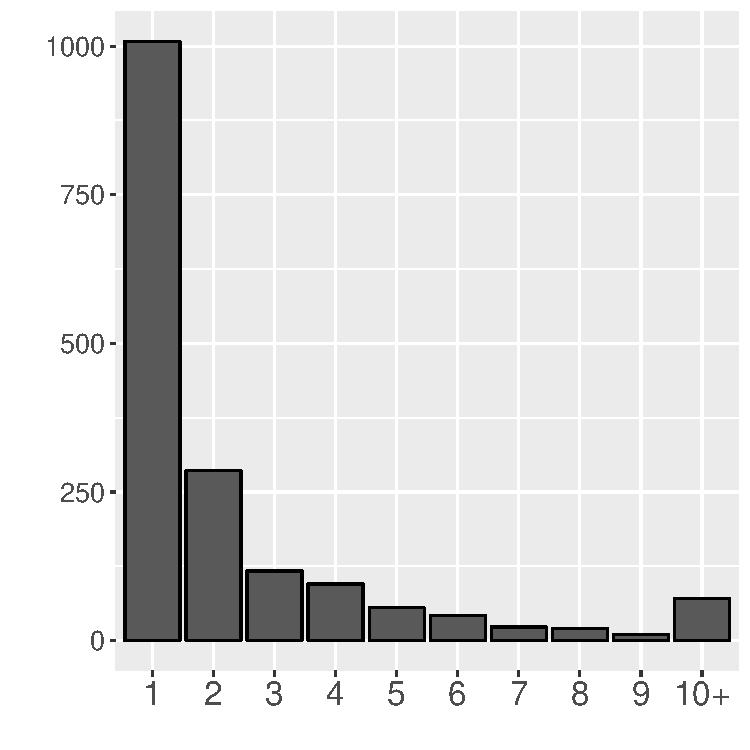
\includegraphics[width=0.7\textwidth]{figure/DiffAll.pdf}
	\caption{Distance from predicate}
	\label{DiffAllF}
%	\end{center}
%\end{minipage}
\end{figure}
\begin{figure}
%\begin{minipage}{0.5\textwidth}
%	\begin{center}
	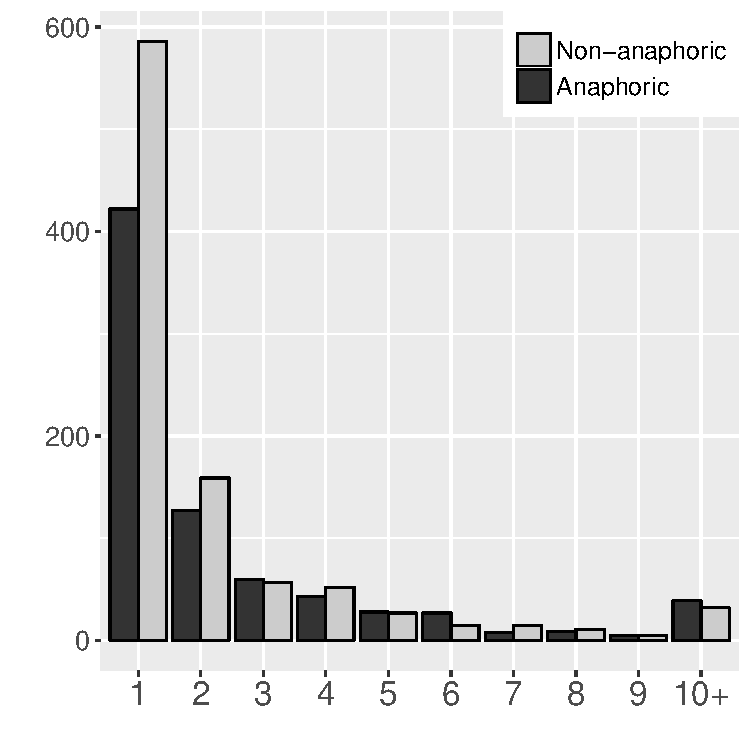
\includegraphics[width=0.7\textwidth]{figure/DiffInfoStatus.pdf}
	\caption{Distance from predicate vs.\ Information status}
	\label{DiffInfoStatusF}
%	\end{center}
%\end{minipage}
\end{figure}
\begin{figure}
%\begin{minipage}{0.5\textwidth}
%	\begin{center}
	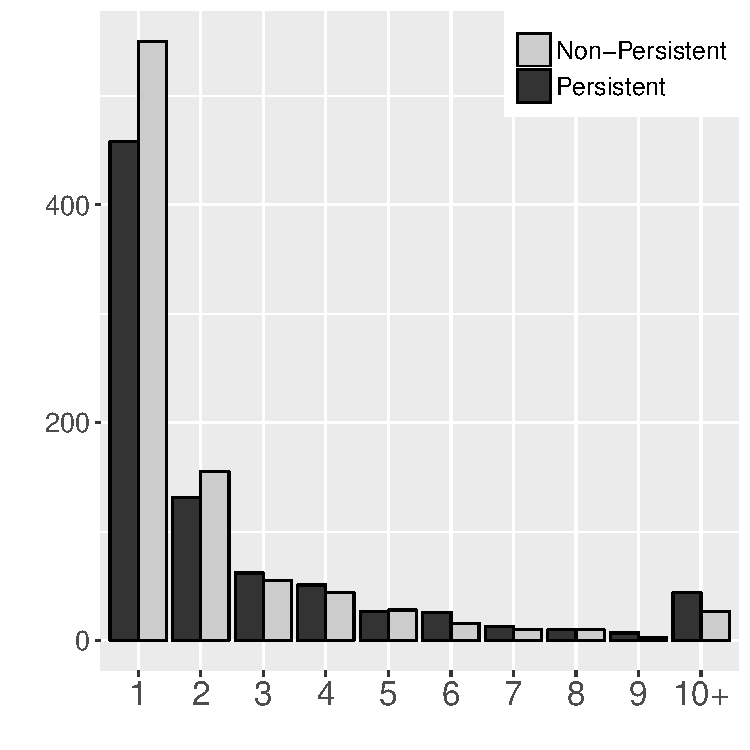
\includegraphics[width=0.7\textwidth]{figure/DiffPersistence.pdf}
	\caption{Distance from predicate vs.\ persistence}
	\label{DiffPerF}
%	\end{center}
%\end{minipage}
\end{figure}

%%----------------------------------------------------
%%----------------------------------------------------
\section{Clause-initial elements}\label{WOSentInitEles}

This section discusses clause-initial elements.
It will be argued that shared elements (i.e., unused, declining, \isi{inferable}, or evoked elements) tend to appear clause-initially
in \S \ref{GivenAppearClause-Initially},
and that
persistent elements tend to appear clause-initially
in \S \ref{PersistentAppearClause-Initially}.
From these observations,
it will be generalized that topics tend to appear clause-initially,
as predicted from the previous literature.
Finally in \S \ref{TopicAppearClause-Initially},
I discuss the motivations for topics to appear clause-initially.


%%----------------------------------------------------
\subsection{Shared elements tend to appear clause-initially}\label{GivenAppearClause-Initially}

%\begin{figure}
%\begin{minipage}{0.5\textwidth}
%	\begin{center}
%	\includegraphics[width=0.95\textwidth]{figure/WO.pdf}
%	\caption{Word order within a clause}
%	\label{WOF}
%	\end{center}
%\end{minipage}
%\begin{minipage}{0.5\textwidth}
%	\begin{center}
%	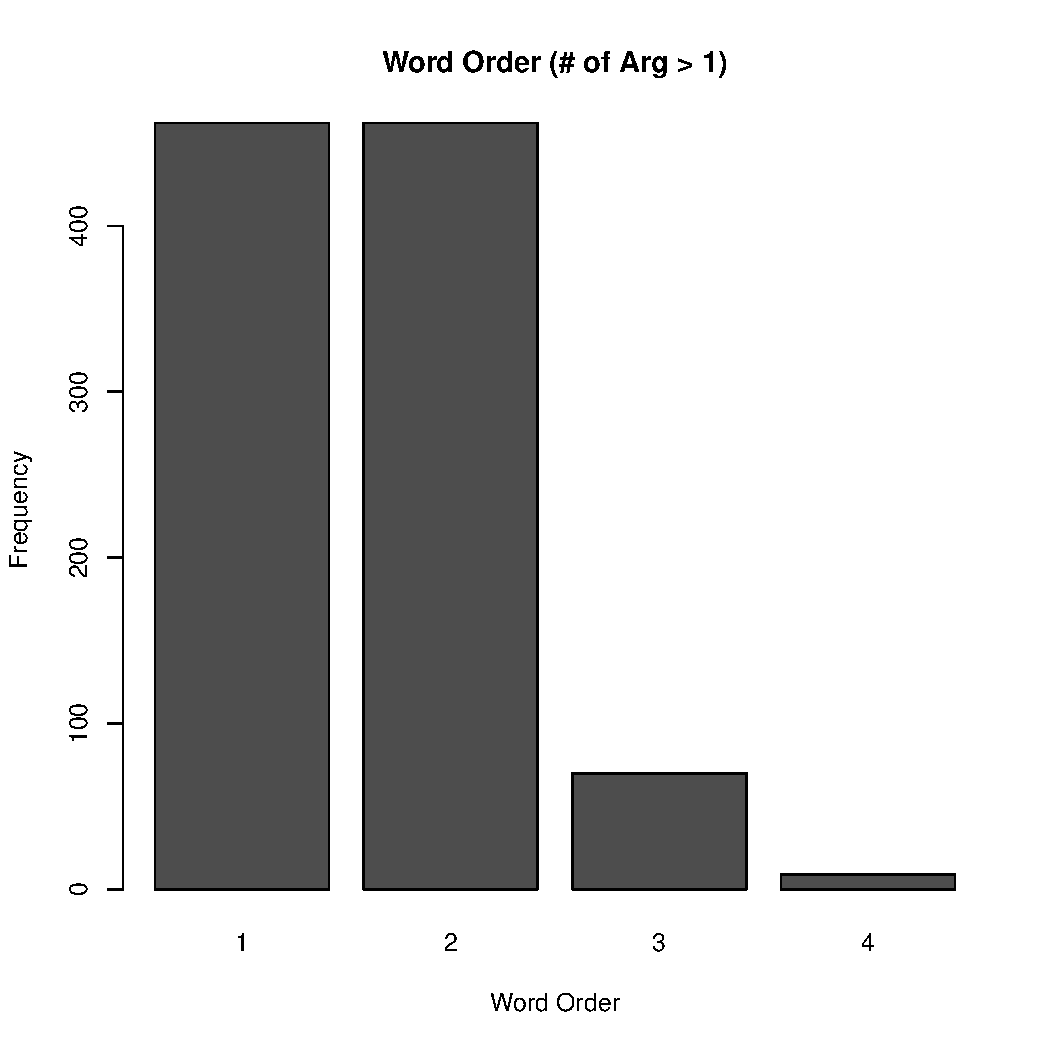
\includegraphics[width=0.95\textwidth]{figure/WO2.pdf}
%	\caption{Word order within a clause (\# of argument $>$ 1)}
%	\label{WO2F}
%	\end{center}
%\end{minipage}

%\begin{minipage}{0.5\textwidth}
%	\begin{center}
%	\includegraphics[width=0.95\textwidth]{figure/WOISGiven.pdf}
%	\caption{Word order vs.\ ASP (given, \# of argument $>$ 1)}
%	\label{WOISGivenF}
%	\end{center}
%\end{minipage}
%\begin{minipage}{0.5\textwidth}
%	\begin{center}
%	\includegraphics[width=0.95\textwidth]{figure/WOISNew.pdf}
%	\caption{Word order vs.\ ASP (new, \# of argument $>$ 1)}
%	\label{WOISNewF}
%	\end{center}
%\end{minipage}
%\end{figure}


Figure \ref{DEPositionISF} shows the frequency of elements and their positions
based on the \isi{information status}.
Anaphoric elements appear most frequently in the third position.
On the other hand, the non-\isi{anaphoric} elements appear most frequently in the fourth position,
but those in the fifth and sixth positions also appear frequently.
%This generalization still holds with another criterion.
%Figure \ref{WOF} shows the position of arguments within a clause (the arguments sharing the same predicate
%%considering only arguments of predicates
%potentially coded by \ci{ga} `\ab{nom}', \ci{o} `\ab{acc}', \ci{ni} `\ab{loc}'%
%	\footnote{
%	In Japanese, the same form \ci{ni} represent both locative and dative.
%	Here I simply included all \ci{ni}-coded elements as arguments.
%	}%
%).
%whereas Figure \ref{WOF} shows the overall orders of arguments.
%In Figure \ref{WOISF},
%clauses where more than one argument appears are considered.
%Figure \ref{WOISGivenF} shows the position of given arguments within a clause, considering only clauses where more than or equal to two arguments appear.
%Figure \ref{WOISNewF} shows the position of new arguments within a clause.
%As shown more clearly in these figures,
%given elements most frequently appear in the initial position,
%while new elements most frequently appear in the second position
%although those in the initial position are still frequent.
These distributions of elements in different information statuses appear to replicate the classic observation that
topics tend to appear earlier in a clause,
i.e., the from-old-to-new principle \cite{mathesius28,firbas64,danes70,kuno78,gundel88}
This is explicitly stated in \Next.
%
\ex. \label{oldnewprinciple}\tl{From-old-to-new principle}:
 In languages in which \isi{word order} is relatively free,
 the unmarked \isi{word order} of constituents is old,
 predictable information first and new, unpredictable information last.
 \hfill{(\citeA[][54]{kuno78}, \citeA[][p.\ 326]{kuno04})}


This principle is motivated by the accumulative nature of processing utterances;
old (or given) elements work as anchors that relate
the previous \isi{utterance} and the following \isi{utterance}.
%This does not indicate that all topics appear sentence initially.
%First,
%some kind of \isi{topic} appear after the predicate rather than at the beginning as will be argued in \S \ref{WORdis},
%where
%the conditions of topics that appear sentence initially and post-predicatively will be discussed.
%Second,
%given foci can also appear at the beginning.
%As shown in \Next, for example,
This principle appears to be supported by examples such as the following.
%\ci{keeki-o} `cake-\ab{acc}' in line (ii),
%which refers to cake and ice cream in line (i),
%can be repeated after \ci{hee}
%and be treated as news.
%\ci{Keeki-o} `keeki-\ab{acc}' can also appear naturally before the predicate as shown in (ii)$^{\prime}$.
%%
%\ex. \a. \ag. koko-ni keeki-to aisu-ga oi-te at-ta-n-da-kedo \\
%		here-\ab{loc} cake-and ice.cream-\ab{nom} put-and exist-\ab{past}-\ab{nmlz}-\ab{cop}-though \\
%		`There were a piece of cake and ice cream,'
%	\bg. \EM{keeki-o} hanako-ga tabe-tyat-ta mitai \\
%		cake-\ab{acc} Hanako-\ab{nom} eat-\ab{pfv}-\ab{past} apparently \\
%		`but Hanako ate the cake.'
%	\bg.[(ii)$^{\prime}$] hanako-ga \EM{keeki-o} tabe-tyat-ta mitai \\
%		Hanako-\ab{nom} cake-\ab{acc} eat-\ab{pfv}-\ab{past} apparently \\
%		`but Hanako ate the cake.'
% \z.
% \b. hee, \{\EM{keeki-o} / Hanako-ga\}
%
In \Next,
\ci{sore} `it' in line c, referring back to \ci{kasi-pan} `sweetbread' in line b, precedes the A element \ci{oziityan} `grandfather'.
%
\ex. \label{PronIni1}
% \ag. sarani uti-no sohu-tteiuno-ga okasi-ga sukina mono-de \\
%   moreover \ab{1}\ab{pl}-\ab{gen} 
% \a. In addition, my grandfather likes sweets,
 \ag. uti-no sohu-tteiuno-ga okasi-ga sukina mono-de \\
 		out-\ab{gen} grandfather-\ci{toiuno}-\ci{ga} sweet-\ci{ga} favorite thing-\ab{cop} \\
		`Our grandfather likes sweets.'
 \bg. yoku pan-ya-san-de \EMi{kasi-pan}-o kat-te kuru-n-desu-ga \\
   often bread-store-\ab{hon}-\ab{loc} sweet-bread-\ci{o} buy-and come-\ab{nmlz}-\ab{cop}.\ab{plt}-though \\
   `(He) often buys sweet bread and comes home,'
 \bg. e n \EM{sore-o} i maa yoowa \EMi{oziityan-wa} issyookenmee \fbox{taberu}-n-desu-keredomo \\
   \ab{fl} \ab{frg} it-\ci{o} \ab{frg} \ab{fl} in.a.word grandfather-\ci{wa} trying.best eat-\ab{nmlz}-\ab{cop}.\ab{plt}-though \\
   `that, he tries his best to eat it, but'
 \b. he cannot eat all and
 \b. gives leftovers to the dog...
  \hfill{(\code{S02M0198: 244.48-262.82})}
%S02M0198|00244484L|244.484271|252.337563|L|更に(0.433)うちの(0.569)祖父っていうのが(0.6)お菓子が好きなもの(0.204)で(0.39)よくパン屋さんで菓子パンを買ってくるんですが|/並列節ガ/|
%S02M0198|00253226L|253.226374|254.606404|L|買い過ぎてしまいまして|/テ節/|
%S02M0198|00255210L|255.209674|272.289576|L|(F え)(F ん)(0.648)それを(D い)(0.147)(F まー)要はお爺ちゃんは一生懸命食べるんですけれども(0.412)余って(0.268)それを犬に(0.194)あげ(0.315)てしまうので(1.403)(F その)残飯で太り(0.447)菓子パンで太り(0.696)味は覚えてグルメになるという最悪の(0.322)育ち方をしてしまいまして|/テ節/|
%

Note that \ci{sore} `it' in line c is not coded by \ci{wa} but by \ci{o}.
This shows that clause-initial shared elements are not necessarily coded by \isi{topic} markers,
although it is predicted that elements coded by \isi{topic} markers would be more likely to appear clause-initially than those coded by case markers (see the discussion in \S \ref{WO:ClauseInit:Ident:Topic}).

Similarly in \Next,
\ci{sore} `it' in line c refers back to \ci{buraunkan} `cathode ray tube'
and appears at the beginning of the clause,
preceding other elements.
%
\ex.\label{PronIni2}
 \ag. oo-gata-no-ne \\
   large-type-\ab{gen}-\ab{fp} \\
   `(It's) a larger type (of cathode ray tube).'
 \bg. yoku maa a hooru-toka-ni aru-yoona oo-gata-no ee {\EMi{buraunkan}}-nan-da-kedomo \\
   often \ab{fl} \ab{fl} hall-etc.-\ab{dat} exist-like large-tyle-\ab{gen} \ab{fl} cathode.ray.tube-\ab{nmlz}-\ab{cop}-though \\
   `(It's) a large type of cathode ray tube typically equipped in a large hall, and'
 \bg. \EM{sore-o}-ne koo \EMi{kotti-kara} \EMi{kotti-ni} \fbox{moti-ageru}-toiu-yoona \\
  that-\ci{o}-\ab{fp} this.way here-from here-from bring-rise-\ab{quot}-like \\
  `this (cathode ray tube), (people) brought it from here to there.'
  \b. some people were doing something like that.
   \hfill{(\code{S05M1236: 471.26-490.38})}

%S05M1236|00462313L|462.313166|477.177522|L|(F ま)ブラウン管て言ってもですね(0.24)(F あのー)小型のブラウン管ではなくて(0.732)(F えー)(0.728)プロジェクション(F えー)チューブっつって(0.377)大きい(0.107)大型のね(0.135)よく(F まー)(F あ)(0.387)ホールとかに(0.134)あるような大型の(1.01)(F えー)ブラウン管なんだけども|/並列節ケドモ/|
%S05M1236|00477852L|477.851579|490.382975|L|(D す)それをね(0.401)こう(0.348)こっちからこっちに持ち上げると(0.5)いうような(0.155)朝から(0.457)朝から(D い)(0.421)夕方までこう(0.383)こっちからこっちに移すと(0.621)いうような仕事をしてる(F うー)同期の人もいました|[文末]|

However,
this is not the whole story;
there are many counter-examples where non-\isi{anaphoric} precedes \isi{anaphoric}.%
%%%ISSUE "where" out of alignment.
Table \ref{GNT} shows the number of cases
where \isi{anaphoric} precedes non-\isi{anaphoric} and non-\isi{anaphoric} precedes \isi{anaphoric} within the same clause.
There are 102 cases where \isi{anaphoric} precedes non-\isi{anaphoric},
while there are 63 cases where non-\isi{anaphoric} precedes \isi{anaphoric}.
The cases where \isi{anaphoric} precedes non-\isi{anaphoric} only slightly outnumber the cases where non-\isi{anaphoric} precedes \isi{anaphoric}.
63 cases (39.4\%) is too large a number to believe that
they are mere exceptions to the principle \ref{oldnewprinciple}.

\begin{table}
\centering
	\caption{Order of anaphoric \& non-anaphoric elements}
\begin{tabular}{rr}
	\toprule
	Anaphoric $\to$ Non-\isi{anaphoric} & Non-\isi{anaphoric} $\to$ Anaphoric \\
	\hline
	102 & 63 \\
	\bottomrule
\end{tabular}
	\label{GNT}
\end{table}

I do not claim that the principle \ref{oldnewprinciple} is not correct,
but I do claim that the principle does not apply to all cases.
Anaphoric elements precede non-\isi{anaphoric} elements
if the \isi{anaphoric} elements are assumed to refer to the ``same'' entity which has been already mentioned.
In other words,
shared elements precede non-\isi{anaphoric} elements.
%I argue that identifiability is also one of the features of topichood.
%What I mean by ``topical'' is that an element has features that correlate with \isi{topic} according to (\ref{ISFeatures}) in Chapter \ref{Framework}.
%In this case,
%being definite is a correlating feature with \isi{topic} and definite elements are called ``topical''.
For example, in \Next,
\ci{mizu} `water' is repeatedly mentioned in the \isi{utterance},
but it is never produced clause-initially.
I argue that this is because
\ci{mizu} `water' in \Next[b] and later is not assumed to refer to the ``same'' entity already mentioned in the previous \isi{discourse}.
%
\ex.\label{WO:ClauseInit:Given:mizu}
 \ag. desukara daitai iti-niti-ni ni-rittoru-no \EM{mizu-o} \ul{tot}-te kudasai-to iw-are-te \\
 so approximately one-day-for two-liter-\ab{gen} water-\ci{o} drink-and please-\ab{quot} tell-\ab{pass}-and \\
 `So we were told to drink two liters of water per day,'
 \bg. syokuzi-no toki-wa kanarazu magukappu-de ni-hai-bun-no \EM{mizu-o} \ul{nomi}-masu-si \\
 	meal-\ab{gen} time-\ci{wa} surely mug-with two-cup-amount-\ab{gen} water-\ci{o} drink-\ab{plt}-and \\
	`whenever we have a meal, we drink two cups of water,'
 \bg. totyuu totyuu-de-mo kanarazu \EM{mizu-o} ho anoo \ul{nomi}-taku-naku-temo \\
 		on.the.way on.the.way-\ab{loc}-also surely water-\ci{o} \ab{frg} \ab{fl} drink-want-\ab{neg}-even.if \\
		`also on the way, even if we didn't want to drink water,'
 \bg. nom-as-areru-to iu kanzi-de \\
 	drink-\ab{caus}-\ab{pass}-\ab{quot} say feeling-\ab{cop} \\
	`we were forced to drink (water).'
 \b. they think that drinking water is very important.
  \hfill{(\code{S01F0151: 339.78-366.29})}
%S01F0151|00339776L|339.775512|341.443878|L|でこのティータイムなんですけれども|/並列節ケレドモ/|
%S01F0151|00341699L|341.698978|349.557717|L|この(0.43)標高の高いところでは(0.141)高山病という非常に危険な(0.329)可能性があるので(0.243)(F えー)水が非常に重要になります|[文末]|
%S01F0151|00349955L|349.954875|366.290044|L|ですから大体一日に二リットルの水を取ってくださいと言われて(0.316)食事の時は必ずマグカップで二杯分の水を(0.145)飲みますし(0.285)途中途中でも必ず水を(0.113)(D ほ)(0.114)(F あのー)(0.432)飲みたくなくても飲まされるという感じで(0.403)水分補給(0.297)を(0.632)重視しておりました|[文末]|


In the same way,
\ci{tenkan} `epilepsy' appears many times in \Next,
but never appears clause-initially.
%
\ex.\label{WO:ClauseInit:Given:tenkan}
 \ag. ato ik-kai \EM{tenkan} \EMi{okosi}-tara sinu-tte it-te-ta-n-desu-kedo \\
      moreover one-time.\ab{cl} epilepsy cause-\ab{cond} die-\ab{quot} say-\ab{past}-\ab{nmlz}-\ab{cop}.\ab{plt}-though \\
      `(The doctor) said that, if (my dog) gets an epilepsy seizure once more, (the dog) would die, but...'
 \bg. mata so sookoo si-teru uti-ni \EM{tenkan} \EMi{okosi}-masi-te \\
      again \ab{frg} meanwhile do-\ab{prog} while-\ab{dat} epilepsy cause-\ab{plt}-and \\
      `meanwhile, (the dog) has an epilepsy seizure, and...'
 \b. The dog recovered this time, but has an epilepsy seizure several times and finally died. (130.8 sec omitted.)
 \bg. sono boku-ga dekakeru toki-ni moo noki-sita-de \EM{tenkan} \EMi{okosi}-te \\
      \ab{fl} \ab{1}\ab{sg}-\ci{ga} go.out when-\ab{dat} already eave-under-\ab{loc} epilepsy cause-and \\
      `When I leave (home), (the dog) had already had an epilepsy seizure, and...'
 \bg. tabun sin-dei-ta-n-da-roo-to \\
      probably die-\ab{prog}-\ab{past}-\ab{nmlz}-\ab{cop}-\ab{infr}-\ab{quot}\\
      `probably died...'
 \bg. ta noki-sita-de \EM{tenkan} \EMi{okosi}-ta-ga tame-ni \\
      \ab{frg} eave-under-\ab{loc} epilepsy cause-\ab{past}-\ab{gen} reason-\ab{dat} \\
      `just because (the dog) has an epilepsy seizure under the eaves...'
 \b. the dog could not get out of there and died, we [the family members] were talking like that.
 \src{S02M0198: 558.7-712.8}
%  \ex [飼い犬が]あと一回\EM{てんかん}起こしたら死ぬって言ってたんですけど
%  \ex またそそうこうしてるうちに\EM{てんかん}起こしまして
%  \ex ... (130.8秒省略。このときは復活したがその後数回てんかんを繰り返し、死んでしまう。)
%  \ex \label{ExTenkan3} その僕が出掛ける時にもう軒下で\EM{てんかん}起こして
%  \ex 多分死んでいたんだろうと
%  \ex \label{ExTenkan4} (た)軒下で\EM{てんかん}起こしたが為に
%  \ex その要は出られなくて
%  \ex 引っ掛かっちゃって
%  \ex 出られなくてそのまま死んじゃったんじゃないのっていう話をしたんですけど\\
%\src{S02M0198: 558.7-712.8}


Whether the speaker refers to the shared entity mentioned previously
depends on the speaker's subjective judgement rather than on objective reasoning.
In \Next, for example,
the \isi{anaphoric element} \ci{kuruma} `car' in line c does not appear clause-initially for the same reason as in \LLast and \Last.
However, \ci{kuruma} `car' in line b and d are clearly the same entity.
%
\ex.\label{WO:ClauseInit:Given:kuruma}
 \ag. kirauea-kazan-mo mappu-o kai-masi-te \\
 		Kilauea-volcano-also map-\ci{o} buy-\ab{plt}-and \\
		`Also for Kilauea, (we) bought a map and'
 \bg. de zibun-tati-de ma rentakaa \EM{kuruma-o} \ul{tobasi}-te e iki-masi-ta \\
 		then self-\ab{pl}-by \ab{fl} rent-a-car car-\ci{o} drive-and \ab{fl} go-\ab{plt}-\ab{past} \\
		`(we) drove there by rent-a-car by ourselves.'
 \b.[] (83.52 sec talking about the mountain.)
 \bg. de anoo jibun-no koko koko-de tyotto tome-te miyoo-to omot-ta toko-ni koo \EM{kuruma-o} \ul{tome}-te \\
 		and \ab{fl} self-\ab{gen} \ab{frg} here-\ab{loc} a.bit stop-and try-\ab{quot} think-\ab{past} place-\ab{dat} this.way car-\ci{o} stop-and \\
	 	`At the place (we) wanted to stop, (we) stopped the car,'
 \b. you can take pictures and so on.
 \hfill{(\code{S00F0014: 843.23-940.34})}
%
%S00F0014|00843233L|843.23315|850.162512|L|(F あのー)キラウエア火山もマップを買いましてで自分達で(0.363)(F ま)レンタカー(0.102)車を(0.376)飛ばして(0.367)(F え)行きました|[文末]|
% ...
%S00F0014|00933685L|933.684509|940.33856|L|で(0.299)(F あのー)自分のここここでちょっと止めてみようと思ったとこにこう車を止めて(0.398)(F まー)その写真を撮ったり|<タリ節>|大きい切れ目−係り先なし

I argue that, in this case, the speaker does not care about the identity of the car.
Rather, she focuses on talking about her trip to Kirauea;
the car she was in is not important for this speech.
As will be discussed in \S \ref{PersistentAppearClause-Initially},
importance, as well as the identity, of the entity contributes to \isi{word order} in spoken Japanese.
Important (i.e., persistent) elements appear clause-initially.

Interestingly,
these elements which are repeatedly mentioned but never appear clause-initially are not referred to by zero or overt pronouns.
It is especially difficult to zero-pronominalize \ci{tenkan} `epilepsy' in \LLast[b-f] and \ci{kuruma} `car' in \Last[d].%
 \footnote{
 It is difficult to apply this test in \ref{WO:ClauseInit:Given:mizu} because \ci{mizu} `water' accompanies numeral modifiers such as 
 `of two liters' and `two cups of'.
 }
Zero pronouns are considered to be the most accessible topics \cite[17]{givon83}.
To zero-pronominalize,
the speaker needs to provide signals to let the \isi{hearer} know which is the \isi{topic}, as will be discussed in \ref{TopicAppearClause-Initially}.

%%
%\ex.
% \ag. koko-ni kuri-gohan-to yaki-zakana-ga oi-te at-ta-kara minna-de tabe-yoo-to omot-ta-n-da-kedo \\
% 		here-\ab{loc} chestnut-rice-and baked-fish-\ab{nom} put-and exist-because all-by eat-will-\ab{quot} think-\ab{past}-\ab{nmlz}-\ab{cop}-though \\
%		`Here there had been chestnut rice and baked fish and I wanted to eat them with everybody, but'
% \bg. \EM{gohan-\{o/wa/{\O}\}} hanako-ga tabe-tyat-ta-n-da-tte \\
% 		rice-\{\ab{acc}/\ci{wa}/{\O}\} Hanako-\ab{nom} eat-\ab{pfv}-\ab{past}-\ab{nmlz}-\ab{cop}-\ab{rep} \\
%		`Hanako ate the rice (and the rice is gone).'
% \bg.[b$^{\prime}$.] hanako-ga \EM{gohan-\{?o/??wa/{\O}\}} tabe-tyat-ta-n-da-tte \\
% 		Hanako-\ab{nom} rice-\{\ab{acc}/\ci{wa}/{\O}\} eat-\ab{pfv}-\ab{past}-\ab{nmlz}-\ab{cop}-\ab{rep} \\
%		`Hanako had eaten meal (so we cannot eat together).'
%%%% イントネーションも重要。b'で「ごはん」に強勢があると、indefiniteとしか解釈されない。
%
%Although the judgement is subtle,
%in \Last[b], where \ci{gohan} `rice' precedes the agent `Hanako',
%\ci{goahn} `rice' inclines to be interpreted as \ci{kuri-gohan} `chestnut rice' which has appeared in the previous line a.
%On the other hand,
%in \Last[b$^{\prime}$], where \ci{gohan} `rice' is preceded by the agent `Hanako',
%\ci{gohan} `rice' inclines to be interpreted as meal in general.%
%	\footnote{
%	In Japanese, \ci{gohan} `rice' is ambiguous between rice and meal in general.
%	}
%Moreover,
%\ci{o}-, \ci{wa}- and zero-codings are possible in \Last[b],
%whereas only zero-coding is natural in \Last[b$^{\prime}$].
%In \Last, \ci{o}-coding is possible because it is separated from the predicate.
%In spoken Japanese,
%P elements tend to be overtly coded if they are separated from the predicate \cite{fry01}.
%\ci{Wa}-coding is possible because \ci{gohan} `rice' appeared in the previous \isi{discourse}.
%I believe the \isi{zero particle} in this case is {\O$_{t}$},
%which is felicitous regardless of the \isi{activation status} of the referent of \ci{gohan} `rice'.
%The \isi{information structure} of \Last[a] can be represented as \Next.
%%
%\ex.
%% \ag. [gohan-o hanako-ga tabe-tyat-ta]$_{F}$ \\
%%			rice-\ab{acc} Hanako-\ab{nom} eat-\ab{pfv}-\ab{past} \\
%	\ag.  [gohan-\{o/wa/{\O}\}]$_{T}$ [hanako-ga tabe-tyat-ta]$_{F}$ \\
%			rice-\{\ab{acc}/\ci{wa}/{\O}\} Hanako-\ab{nom} eat-\ab{pfv}-\ab{past} \\
%
%I argue that \ci{o}-coded \ci{gohan} `rice' in the initial position is still \isi{topic} to some extent,
%although it is not coded by the \isi{topic} marker \ci{wa};
%P in the initial position, preceding focus A,
%only refers to elements which has been activated in the \isi{hearer}'s mind.
%\LLast[b] cannot receive the interpretation \LLast[b$^{\prime}$].
%If this position is for focus, there should be no such constraint;
%focus is by default non-\isi{anaphoric} and has not been activated in the \isi{hearer}'s mind.
%Moreover, most given Ps are still coded by \ci{o} `\ab{acc}' as will be discussed below.
%
%In \LLast[b$^{\prime}$], on the other hand,
%\ci{gohan} `rice' cannot be coded by \ci{o} or \ci{wa}.
%Assuming that the \isi{information structure} of \Last[b] is \Next,
%\ci{gohan} is felicitously coded by \ci{o} `\ab{acc}' because
%\isi{non-contrastive focus} P elements cannot felicitously coded by \ci{o}.
%\exg. [hanako-ga gohan-{\O} tabe-tyat-ta]$_{F}$ \\
%		Hanako-\ab{nom} rice-{\O} eat-\ab{pfv}-\ab{past} \\
%
%I claim \ci{wa}-coding is impossible because
%of the incompatible characteristics of \ci{wa}-coding and the element's position;
%\ci{wa} codes activated element at issue and the element between the focus agent and the focus predicate is also interpreted as focus.
%Since focus elements are tend to be \isi{indefinite} and non-\isi{anaphoric},
%\ci{gohan} `rice' in \LLast[b$^{\prime}$] inclines to be interpreted as \isi{indefinite} and new.
%Still, I claim that \ci{gohan-o} `rice-\ab{acc}' in \LLast[b] is focus but given
%because it appears in the initial position preceding other focus elements.

%This claim seems difficult to test in the corpus because
%there is no definite markers in Japanese.
From the discussion above,
there are at least two predictions testable in the corpus.
Firstly, since evoked and \isi{inferable} elements are coded by \isi{topic} markers, as was shown in Chapter \ref{Particles},
it is predicted that
elements coded by \isi{topic} markers tend to appear earlier in a clause (\S \ref{WO:ClauseInit:Ident:Topic}).
This is because elements assumed by the speaker to be evoked or \isi{inferable}
are also assumed to be shared.
Secondly,
since pronouns essentially code shared elements which have been mentioned,
pronouns are also predicted to appear earlier in a clause (\S \ref{WO:ClauseInit:Ident:Pron}).
Both predictions are confirmed in the following investigations.
Thirdly, I will show that clause-initial elements are not sensitive to \isi{activation cost};
unused elements can also appear clause-initially (\S \ref{WO:ClauseInit:Ident:ActStatus}).
Evoked, \isi{inferable}, declining, and unused elements are shared
(See Table \ref{ActStatusCorpus}).
Therefore, the claim that shared elements appear clause-initially is supported.

%%----------------------------------------------------
\subsubsection{Topic-coded elements appear clause-initially}\label{WO:ClauseInit:Ident:Topic}

\begin{figure}
%\begin{minipage}{0.5\textwidth}
	\begin{center}
	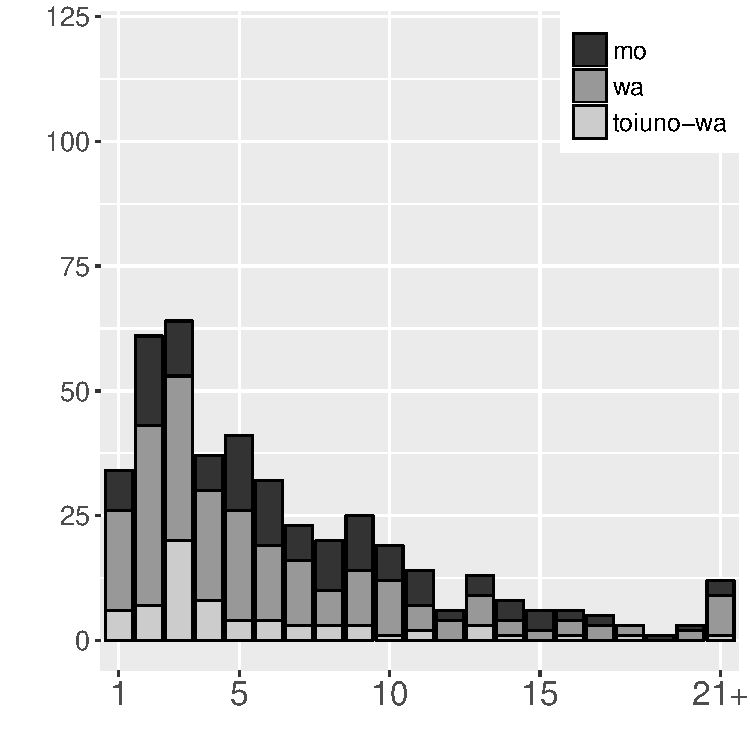
\includegraphics[width=0.7\textwidth]{figure/WOTopPar.pdf}
	\caption{Order of arguments coded by topic markers}
	\label{WOTopParF}
	\end{center}
%\end{minipage}
\end{figure}
\begin{figure}
%\begin{minipage}{0.5\textwidth}
	\begin{center}
	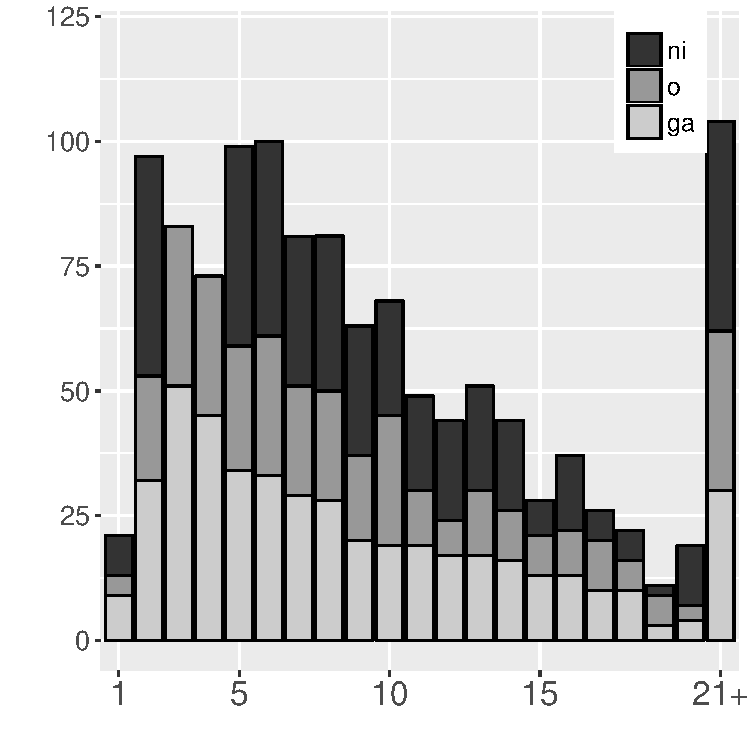
\includegraphics[width=0.7\textwidth]{figure/WOCasePar.pdf}
	\caption{Order of arguments coded by case markers}
	\label{WOCaseParF}
	\end{center}
%\end{minipage}
\end{figure}

%%% \ref{Par:ArgStr}で一部議論重複
Let us test the prediction that elements coded by \isi{topic} markers tend to appear earlier in a clause.
Figure \ref{WOTopParF} shows the distribution of topic-coded elements
and their positions.
Compare this figure with Figure \ref{WOCaseParF},
which shows the distribution of case-coded elements and their positions.
It is clear that
elements coded by \isi{topic} markers are more skewed to earlier positions within a clause as compared to those coded by case markers.

\Next is an example of a \ci{wa}-coded element appearing clause-initially.
The \ci{wa}-coded element \ci{hone} `bone' in line a,
which has been discussed in the previous \isi{discourse},
is separated from the predicate by an intervening locative (a tomb for animals in the temple).
The intervening part is long and the predicate finally appears in line d.
%
\ex.
	\ag. ee suriipii-no itibu-no oo \EM{hone-wa} \\
		\ab{fl} Sleepy-\ab{gen} part-\ab{gen} \ab{fl} bone-\ci{wa} \\
		`Part of bone of Sleepy (dog's name),'
	\bg. sono morimati-no watasi-no senzo-no o hait-teru otera-no \\
		that Morimachi-\ab{gen} \ab{1}\ab{sg}-\ab{gen} ancestor-\ci{gen} \ab{fl} enter-\ab{prog} temple-\ab{gen} \\
		`the temple in Morimachi where my ancestors were,'
	\bg. yahari ano doobutu-no kuyootoo-ga ari-masu \\
		again that animal-\ab{gen} tomb-\ci{ga} exist-\ab{plt} \\
		`there are tombs for animals,'
	\bg. sotira-no hoo-ni \ul{osame}-masite-ne \\
		that-\ab{gen} direction-\ab{dat} place-\ab{plt}-and \\
		`(we) placed (his bone) there.'
	\hfill{(\code{S02M1698: 620.12-634.26})}
%S02M1698|00620119L|620.118778|634.26275|L|(F えー)スリーピーの一部の(0.379)(F おー)骨は(0.438)その<FV>森町の(0.669)私の先祖の(0.598)(F お)入ってるお寺の(0.465)やはり(F あの)動物の供養塔があります(0.358)そちらの方に納め(0.347)ましてね|/テ節/|

In \Next,
\ci{sono ko} `that puppy',
whose referent has appeared in the previous line a,
is also an example of a \ci{wa}-coded element appearing clause-initially.
The element is also separated from the predicate
by an intervening argument `distemper'.
%
\ex.
	\ag. mosi \EMi{koinu-o} kat-tesimat-tara \\
		if puppy-\ci{o} keep-\ab{pfv}-\ab{cond} \\
		`If you decided to keep a new puppy,'
	\bg. \EM{sono} \EM{ko-wa} mata zisutenpaa-ni \ul{kakat}-te sin-zyau-kara \\
			that puppy-\ci{wa} again distemper-\ab{dat} catch-and die-\ab{pfv}-because \\
			`the puppy will die of distemper again, so'
	\b. keep a new puppy after this winter, this is what we were told by the vet.
	\hfill{(\code{S02M0198: 108.68-126.70})}
%
%S02M0198|00108681L|108.680591|126.700531|L|冬を越さないと(0.407)ジステンパーの細菌が(0.47)庭にいるままで死んでくれないから(0.431)もし小犬を飼っ(0.843)てしまったら(0.382)その子はまたジステンパーに掛かって死んじゃうから(0.584)冬を越してから(0.403)新しい犬を飼ってくれ(0.356)と僕らは言われていたもので|<並列節デ>|大きい切れ目−係り先なし

%\Next is an example of given elements that are neither coded by \isi{topic} markers nor put in clause-initially.
%The element \ci{mizu} `water' appears three times in \Next,
%all of which are given.
%\ex.\label{WO:Ex:mizu}
% \ag. desukara daitai iti-niti-ni ni-rittoru-no \EM{mizu-o} \ul{tot}-te kudasai-to iw-are-te \\
% so approximately one-day-for two-liter-\ab{gen} water-\ab{acc} drink-and please-\ab{quot} tell-\ab{pass}-and \\
% `So we were told to drink two liters of water per day,'
% \bg. syokuzi-no toki-wa kanarazu magukappu-de ni-hai-bun-no \EM{mizu-o} \ul{nomi}-masu-si \\
% 	meal-\ab{gen} time-\ci{wa} surely mug-with two-cup-amount-\ab{gen} water-\ab{acc} drink-\ab{plt}-and \\
%	`whenever we have meal, we drink two cups of water,'
% \bg. totyuu totyuu-de-mo kanarazu \EM{mizu-o} ho anoo \ul{nomi}-taku-naku-temo \\
% 		on.the.way on.the.way-\ab{loc}-also surely water-\ab{acc} \ab{frg} \ab{fl} drink-want-\ab{neg}-even.if \\
%		`also on the way, even if we didn't want to drink water,'
% \bg. nom-as-areru-to iu kanzi-de \\
% 	drink-\ab{caus}-\ab{pass}-\ab{quot} say feeling-\ab{cop} \\
%	`we were forced to drink (water).'
% \b. they think that drinking water is very important.
%  \hfill{(\code{S01F0151: 339.78-366.29})}
%%S01F0151|00339776L|339.775512|341.443878|L|でこのティータイムなんですけれども|/並列節ケレドモ/|
%%S01F0151|00341699L|341.698978|349.557717|L|この(0.43)標高の高いところでは(0.141)高山病という非常に危険な(0.329)可能性があるので(0.243)(F えー)水が非常に重要になります|[文末]|
%%S01F0151|00349955L|349.954875|366.290044|L|ですから大体一日に二リットルの水を取ってくださいと言われて(0.316)食事の時は必ずマグカップで二杯分の水を(0.145)飲みますし(0.285)途中途中でも必ず水を(0.113)(D ほ)(0.114)(F あのー)(0.432)飲みたくなくても飲まされるという感じで(0.403)水分補給(0.297)を(0.632)重視しておりました|[文末]|

%I argue that `water' in \Last is interpreted as \isi{indefinite} and the givenness of `water' does not matter in this narrative.
%This is because \ci{mizu} `water' appears non-initial position.
%Of course there are definite referents appearing non-initial position.
%However, the givenness of those referents are still not important.
%Consider the following example.
%%
%\ex.\label{WO:Ex:kuruma}
% \ag. kirauea-kazan-mo mappu-o kai-masi-te \\
% 		Kilauea-volcano-also map-\ab{acc} buy-\ab{plt}-and \\
%		`Also for Kilauea, (we) bought a map and'
% \bg. de zibun-tati-de ma rentakaa \EM{kuruma-o} \ul{tobasi}-te e iki-masi-ta \\
% 		then self-\ab{pl}-by \ab{fl} rent-a-car car-\ab{acc} drive-and \ab{fl} go-\ab{plt}-\ab{past} \\
%		`(we) drove there by rent-a-car by ourselves.'
% \b.[] (83.52 sec talking about the mountain.)
% \bg. de anoo jibun-no koko koko-de tyotto tome-te miyoo-to omot-ta toko-ni \\
% 		and \ab{fl} self-\ab{gen} \ab{frg} here-\ab{loc} a.bit stop-and try-\ab{quot} think-\ab{past} place-\ab{loc} \\
%	 	`At the place (we) wanted to stop,'
% \bg. koo \EM{kuruma-o} \ul{tome}-te \\
% 		this.way car-\ab{acc} stop-and \\
%		`(we) stopped the car,'
% \b. you can take pictures and so on.
% \hfill{(\code{S00F0014: 843.23-940.34})}
%%
%%S00F0014|00843233L|843.23315|850.162512|L|(F あのー)キラウエア火山もマップを買いましてで自分達で(0.363)(F ま)レンタカー(0.102)車を(0.376)飛ばして(0.367)(F え)行きました|[文末]|
%% ...
%%S00F0014|00933685L|933.684509|940.33856|L|で(0.299)(F あのー)自分のここここでちょっと止めてみようと思ったとこにこう車を止めて(0.398)(F まー)その写真を撮ったり|<タリ節>|大きい切れ目−係り先なし
%
%In \Last,
%\ci{kuruma} `car' is mentioned in lines b and d.
%Since it is reasonable to think that the speakers drove the same car while they were travelling,
%\ci{kuruma} `car' in line d is inferred as definite.
%However, the \isi{definiteness} or givenness of the car here is irrelevant to the \isi{discourse};
%the speaker is talking about their travel to Kilauea not about the car.
%Therefore,
%\ci{kuruma} is coded by the \isi{case marker} \ci{o} and appears non-initial position, i.e., immediately before the predicate as will be discussed in \S \ref{WOPrePredEles}.

\ci{Wa} appearing in the initial position is already conventionalized, and
it is possible to test this with acceptability judgements.
It is not acceptable for \ci{wa}-coded P to appear between the focus agent and the predicate except for contrastive readings of \ci{wa}.
%	\footnote{
%	Contrastive \ci{wa} appearing in this position will be
%	discussed more in detail in \S \ref{WODiscussion}.
%	}
As the contrast between \Next[a-c] shows,
the zero-coded P \ci{hon} `book' in \Next[a] right before the predicate is acceptable,
while the \ci{wa}-coded \ci{hon} `book' in the same position in \Next[b] is not acceptable.
To express the idea of \Next[b],
the \ci{wa}-coded P should precede A \ci{taroo} `Taro'.
%
\ex. \ag. \ul{taroo-ga} \EM{hon} yon-deru-yo \\
		Taro-\ci{ga} book read-\ab{prog}-\ab{fp} \\
		`Taro is reading a book.'
	\bg. ??\ul{taroo-ga} \EM{hon-wa} yon-deru-yo \\
		Taro-\ci{ga} book-\ci{wa} read-\ab{prog}-\ab{fp} \\
		`Taro is reading the book.'
	\bg. \EM{hon-wa} \ul{taroo-ga} yon-deru-yo \\
		book-\ci{wa} Taro-\ci{ga} read-\ab{prog}-\ab{fp} \\
		`Taro is reading the book.'
		\hfill{(Constructed)}

There is only one example (out of 9 \ci{wa}-coded Ps) in the corpus
where \ci{wa}-coded P is preceded by \ci{ga}-coded A.
This \ci{wa}-coded P is contrastive, which will be discussed in \S \ref{WODiscussion}.

I propose the hypothesis that elements which belong to the same unit of \isi{information structure} appear adjacent within a clause.
I call this the information-structure \isi{continuity principle} in \isi{word order}.
%
\ex. \label{IScontinuityP}\tl{Information-structure continuity principle}:
 A unit of \isi{information structure} is continuous in a clause;
 i.e., elements which belong to the same unit are adjacent with each other.

This principle explains why \LLast[b] is not acceptable,
while \LLast[a,c] are acceptable.
The \isi{information structure} of each of the examples \LLast is represented in \Next.
In \Next[b],
the \isi{topic} P element \ci{hon-wa} `book-\ci{wa}' intervenes between two focus elements \ci{taroo-ga} `Taro-\ci{ga}' and \ci{yon-deru} `read-\ab{prog}', which is not acceptable.
In \Next[c], on the other hand,
the \isi{topic} P does not split up the domain of focus,
and the whole sentence is acceptable.
In \Next[a],
all the elements including \ci{hon} `book' belong to focus
and hence \ci{hon} in this position is acceptable.
%
\ex. \ag. [\ul{taroo-ga} \EM{hon} yon-deru]$_{F}$-yo \\
		Taro-\ci{ga} book read-\ab{prog}-\ab{fp} \\
		`Taro is reading a book.'
	\bg. ??[\ul{taroo-ga}]$_{F}$ [\EM{hon-wa}]$_{T}$ [yon-deru]$_{F}$-yo \\
		Taro-\ci{ga} book-\ci{wa} read-\ab{prog}-\ab{fp} \\
		`Taro is reading the book.'
	\bg. [\EM{hon-wa}]$_{T}$ [\ul{taroo-ga} yon-deru]$_{F}$-yo \\
		book-\ci{wa} Taro-\ci{ga} read-\ab{prog}-\ab{fp} \\
		`Taro is reading the book.'

Interestingly,
it is possible for \ci{wa}-coded A to be preceded by \ci{o}-coded P, as shown in \Next[a] (compare this with \Next[b]).
%
\ex.
\ag. \ul{hon-o} \EM{taroo-wa}  yon-deru-yo \\
		book-\ci{o} Taro-\ci{wa} read-\ab{prog}-\ab{fp} \\
		`Taro is reading the book.'
\bg. \ul{hon-o} \EM{taroo-ga} yon-deru-yo \\
		book-\ci{o} Taro-\ci{ga} read-\ab{prog}-\ab{fp} \\
		`Taro is reading the book.'

As was argued above,
the preposed P, \ci{hon-o} `book-\ci{o}' in \Last,
is topical, which is represented as in \Next.
%
\ex.
\ag. [\ul{hon-o} \EM{taroo-wa}]$_{T}$  [yon-deru]$_{F}$-yo \\
		book-\ci{o} Taro-\ci{wa} read-\ab{prog}-\ab{fp} \\
		`Taro is reading the book.'
\bg. [\ul{hon-o}]$_{T}$ [\EM{taroo-ga} yon-deru]$_{F}$-yo \\
		book-\ci{o} Taro-\ci{ga} read-\ab{prog}-\ab{fp} \\
		`Taro is reading the book.'

As shown in \Last[a],
the two \isi{topic} elements \ci{hon-o} `book-\ci{o}' and \ci{taroo-wa} `Taro-\ci{wa}' are adjacent to each other and hence this sentence is acceptable.
Also in \Last[b],
the only \isi{topic} element \ci{hon-o} `book-\ci{o}' does not split up the focus elements \ci{taroo-ga yon-deru}, which is predicted to be acceptable.
\ci{Hon-o} `book-\ci{o}' could be focus instead of \isi{topic} in \LLast[b], since given elements can be focus.
But it is reasonable to think of a situation where given focus elements are preposed
for the sentence to be a smooth transition from the previous sentence.
The information-structure \isi{continuity principle} \ref{IScontinuityP} still holds in either case.

Note that \ref{IScontinuityP} does not refer to \isi{word order};
rather, it is about adjacency.
I argue that this principle is also at work in intonation (see Chapter \ref{Intonation}).

What is the difference between clause-initial elements coded by \isi{topic} markers and those coded by case markers?
As was discussed in \S \ref{Par:ArgStr:TopHierarchy},
there is a hierarchy of \isi{topic} coding \ref{ASPGivenSchema},
which is repeated here as \Next.
%
\ex.
 A, S $>$ P

The hierarchy indicates that
evoked or \isi{inferable} A and S are more likely to be coded by \isi{topic} markers than P in the same status.
Word order is not affected by this hierarchy.
Figures \ref{WOSGivenF} and \ref{WOPGivenF} show \isi{word order} of
\isi{anaphoric} S and P, respectively.
Compare these with Figures \ref{WOSNewF} and \ref{WOPNewF},
which show \isi{word order} of non-\isi{anaphoric} S and P.
Word order of A is omitted because the number is too small.
As can be seen from the contrasts between Figures \ref{WOSGivenF} and \ref{WOSNewF} and between Figures \ref{WOPGivenF} and \ref{WOPNewF},
\isi{anaphoric} elements are more likely to appear earlier in a clause than non-\isi{anaphoric} elements.
Although the contrast is less clear between \isi{anaphoric} vs.~non-\isi{anaphoric} P,
especially notable is that there are three times as many \isi{anaphoric} Ps as non-\isi{anaphoric} Ps in the third position.
(There are 27 \isi{anaphoric} Ps in the third position,
while there are only 10 non-\isi{anaphoric} P.)
I speculate that the contrast is less clear in \isi{anaphoric} vs.~non-\isi{anaphoric} P than S because there are cases like \ref{WO:ClauseInit:Given:mizu} and \ref{WO:ClauseInit:Given:tenkan},
where the element is annotated as \isi{anaphoric} but is considered to be not shared.
In this case, P appears pre-predicatively rather than clause-initially.
Therefore, I argue that,
while elements coded by \isi{topic} markers are likely to appear earlier in a clause,
\isi{word order} is independent of \isi{topic} marking.
Topic markers are sensitive to the given-new taxonomy, as was discussed in Chapter \ref{Particles};
clause-initial position is sensitive to sharedness.
Topic markers and \isi{word order} are sensitive to different aspects of topichood.

\begin{figure}
%\begin{minipage}{0.5\textwidth}
	\begin{center}
	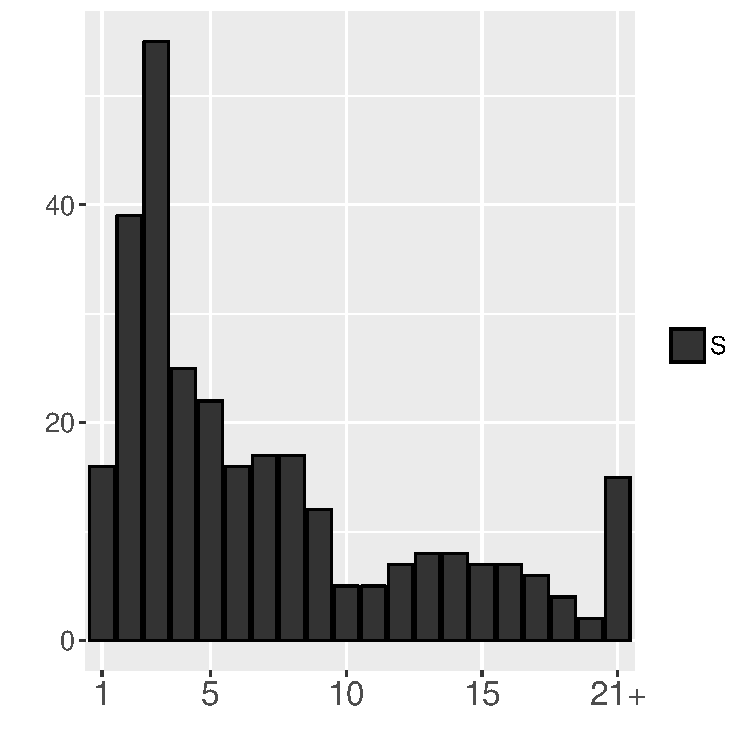
\includegraphics[width=0.6\textwidth]{figure/WOSGiven.pdf}
	\caption{Word order of anaphoric S}
	\label{WOSGivenF}
	\end{center}
%\end{minipage}
\end{figure}
\begin{figure}
%\begin{minipage}{0.5\textwidth}
	\begin{center}
	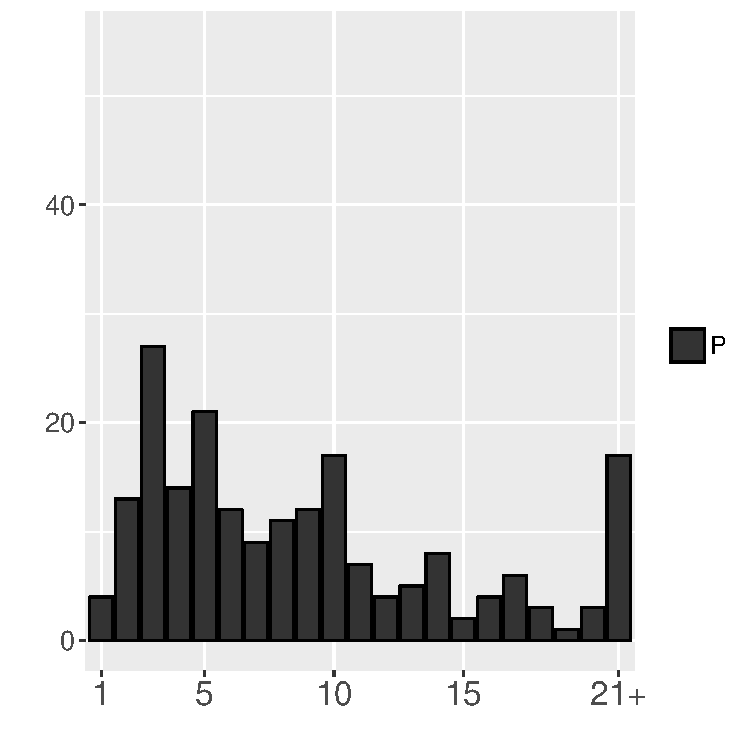
\includegraphics[width=0.6\textwidth]{figure/WOPGiven.pdf}
	\caption{Word order of anaphoric P}
	\label{WOPGivenF}
	\end{center}
%\end{minipage}
\end{figure}
\begin{figure}
%\begin{minipage}{0.5\textwidth}
	\begin{center}
	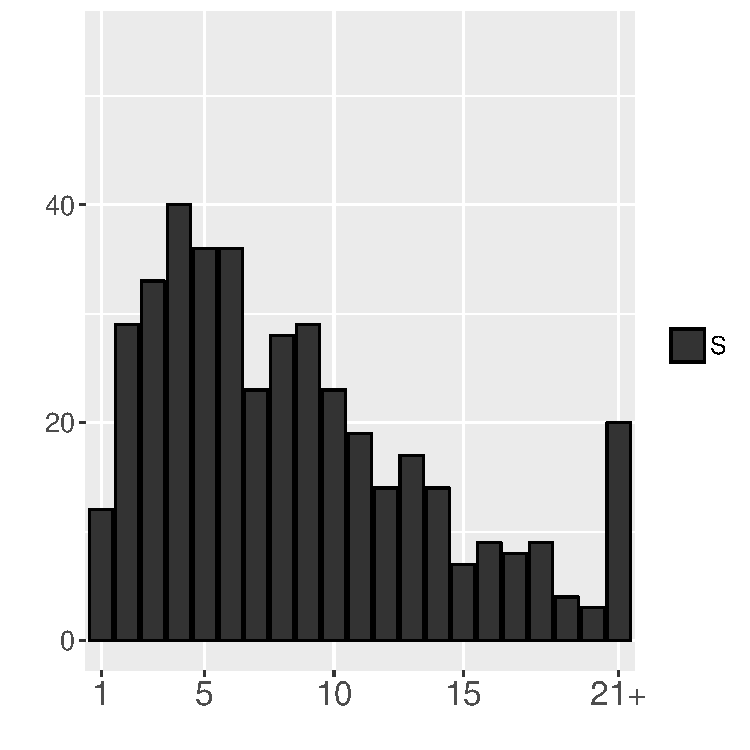
\includegraphics[width=0.6\textwidth]{figure/WOSNew.pdf}
	\caption{Word order of non-anaphoric S}
	\label{WOSNewF}
	\end{center}
%\end{minipage}
\end{figure}
\begin{figure}
%\begin{minipage}{0.5\textwidth}
	\begin{center}
	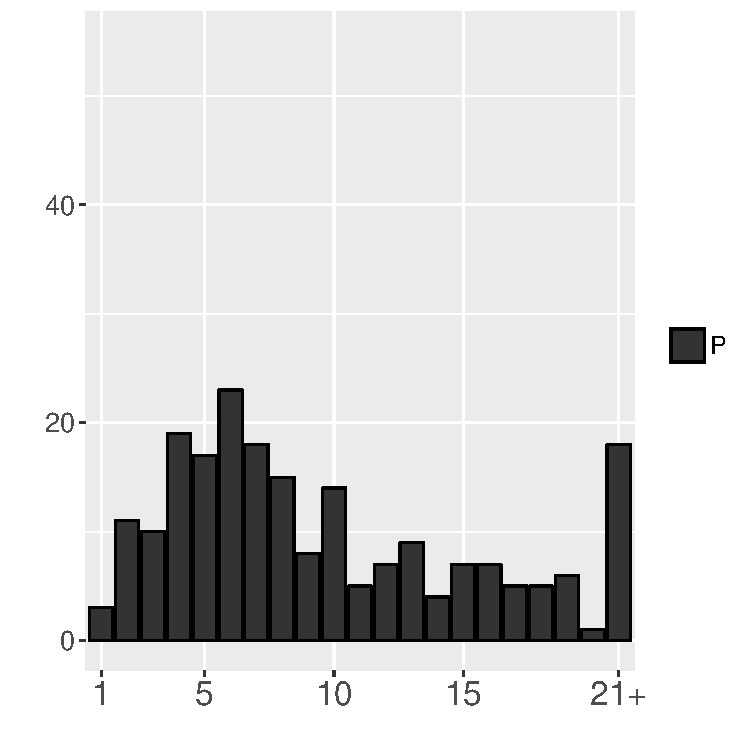
\includegraphics[width=0.6\textwidth]{figure/WOPNew.pdf}
	\caption{Word order of non-anaphoric P}
	\label{WOPNewF}
	\end{center}
%\end{minipage}
\end{figure}

%%----------------------------------------------------
\subsubsection{Pronouns appear clause-initially}\label{WO:ClauseInit:Ident:Pron}

Next let us examine the position of pronouns.
Figure \ref{WOExpTypeF} shows the positions of pronouns.
Figure \ref{DEPositionAllF}, repeated as Figure \ref{DEPositionAllF2} for comparison,
represents the distributions of all elements.
Although the number of pronouns is small,
it is clear, comparing with the overall distributions of elements in Figure \ref{DEPositionAllF2}, that
the order of pronouns is skewed to earlier positions within a clause.
Hence, it is reasonable to conclude that
pronouns are likely to appear earlier in a clause.
Examples of pronouns appearing earlier in a clause are shown in \ref{PronIni1} and \ref{PronIni2} above.
The result is compatible with \citeA{yamashita02} and \citeA{kondoyamashita07}.


\begin{figure}
%\begin{minipage}{0.5\textwidth}
	\begin{center}
	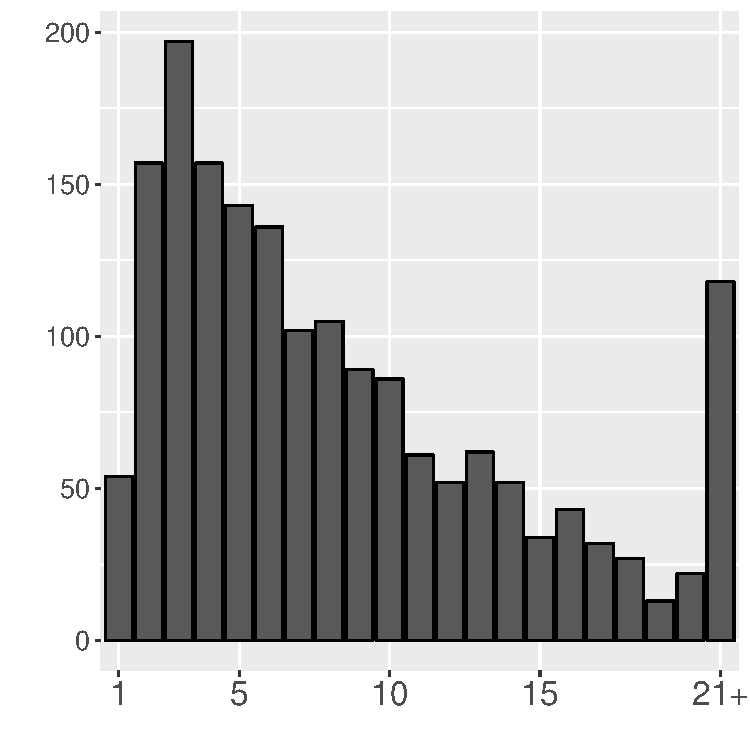
\includegraphics[width=0.6\textwidth]{figure/DEPositionAll.pdf}
	\caption{Order of all elements}
	\label{DEPositionAllF2}
	\end{center}
%\end{minipage}
\end{figure}
\begin{figure}
%\begin{minipage}{0.5\textwidth}
	\begin{center}
	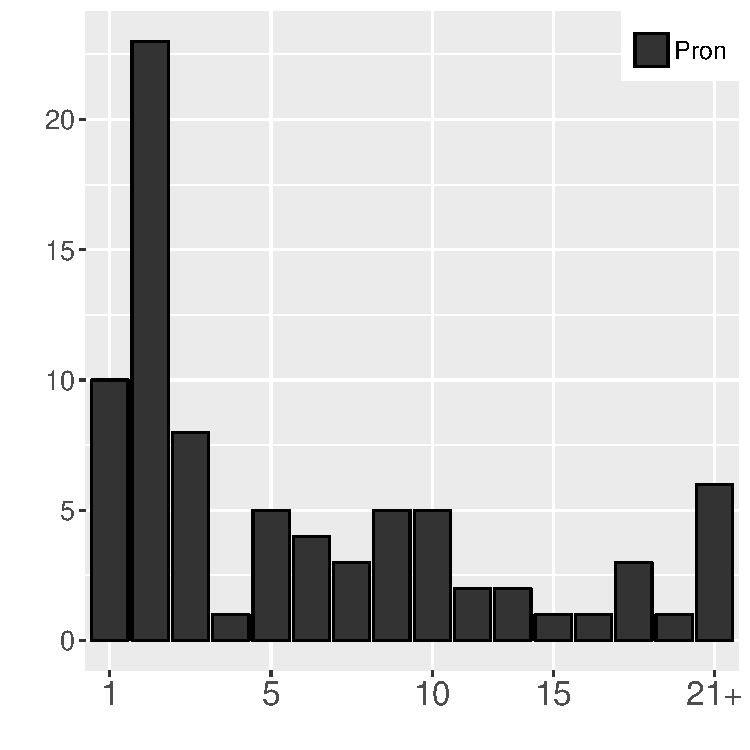
\includegraphics[width=0.6\textwidth]{figure/WOExpType.pdf}
	\caption{Order of pronouns}
	\label{WOExpTypeF}
	\end{center}
\end{figure}

%\begin{table}
%\begin{minipage}{0.5\textwidth}
%\centering
%	\caption{Markers for ASP (given)}
%	\label{ASPParGivenT}
%	\begin{tabular}{lrrr}
%	\toprule
%			 & A & S & P \\
%	\midrule
%	\ci{o} 	& 0 & 0 & 166 \\
%	\ci{ga} 	& 29 & 191 & 0 \\
%	\midrule
%	\isi{case marker} & 29 & 191 & 166 \\
%	  & (50.9\%) & (59.0\%) & (91.2\%) \\
%	\midrule
%	\midrule
%	\ci{wa} 	& 27 & 104 & 14 \\
%	\ci{toiunowa} 	& 1 & 29 & 2 \\
%	\midrule
%	\isi{topic} marker & 28 & 133 & 16 \\
%	  & (49.1\%) & (41.0\%) & (8.8\%) \\
%	\midrule
%	\midrule
%	sum & 57 & 324 & 182 \\
%	  & (100\%) & (100\%) & (100\%) \\
%	\bottomrule
%	\end{tabular}
%\end{minipage}
%\begin{minipage}{0.5\textwidth}
%\centering
%	\caption{Markers for ASP (new)}
%	\label{ASPParNewT}
%	\begin{tabular}{rrr}
%	\toprule
%	A & S & P \\
%	\midrule
%	0 & 0 & 211 \\
%	15 & 351 & 0 \\
%	\midrule
%	15 & 351 & 211 \\
%	(78.9\%) & (76.5\%) & (92.5\%) \\
%	\midrule
%	\midrule
%	3 & 90 & 14 \\
%	1 & 18 & 3 \\
%	\midrule
%	4 & 108 & 17 \\
%	(21.1\%) & (23.5\%) & (7.5\%) \\
%	\midrule
%	\midrule
%	19 & 459 & 228 \\
%	(100\%) & (100\%) & (100\%) \\
%	\bottomrule
%	\end{tabular}
%\end{minipage}
%\end{table}

%%----------------------------------------------------
\subsubsection{Unused elements appear clause-initially}\label{WO:ClauseInit:Ident:ActStatus}

Not only evoked, \isi{inferable}, and declining elements,
but also unused elements appear clause-initially.
Elements coded by the \isi{copula} followed by \ci{ga} or \ci{kedo} are unused elements, as was discussed in Chapter \ref{Particles}.%
 \footnote{
 \chd{See \S \ref{BackSubSubKedo} for the reason why
 an element coded by the \isi{copula} followed by \ci{ga} or \ci{kedo} is not considered to be a clause.}
 }
It is very unnatural when they are preceded by other arguments.
For example,
as shown in the contrast between \Next[a] and \Next[b],
\ci{rei-no ken} `that issue' cannot be felicitously preceded by another argument, in this case \ci{kotira-de} `this side'.
%
\ex.
 \ag. \EM{rei-no} \EM{ken-desu-ga} kotira-de nantoka nari-sou-desu \\
      that-\ab{gen} issue-\ab{cop}.\ab{plt}-though this.side-\ab{loc} whatever become-will-\ab{cop}.\ab{plt} \\
      `Regarding that issue, (I) guess (we) figured the way out.'
      \hfill{\cite[modified from][283]{niwa06}}
 \bg.[a$^{\prime}$.] ??kotira-de \EM{rei-no} \EM{ken-desu-ga} nantoka nari-sou-desu \\
      this.side-\ab{loc} that-\ab{gen} issue-\ab{cop}.\ab{plt}-though whatever become-will-\ab{cop}.\ab{plt} \\

In a similar manner,
\ci{yamada-no koto} `the issue of Yamada' cannot naturally be preceded by an \isi{adverbial}, \ci{ano mama} `that way',
as shown in the contrast between \Next[a] and \Next[b].
%
\ex.
 \ag. \EM{yamada-no} \EM{koto-da-kedo} ano mama hot-toi-te ii-no-kana \\
      Yamada-\ab{gen} issue-\ab{cop} that way leave-let-and good-\ab{nmlz}-\ab{q} \\
      `Regarding Yamada, is it OK to just leave him?'
      \hfill{\cite[283]{niwa06}}
 \bg.[a$^{\prime}$.] ??ano mama \EM{yamada-no} \EM{koto-da-kedo} hot-toi-te ii-no-kana \\
      that way Yamada-\ab{gen} issue-\ab{cop} leave-let-and good-\ab{nmlz}-\ab{q} \\


Unused elements include \isi{indefinite} elements
although it is counter-intuitive to consider \isi{indefinite} NPs as being ``shared''.
For example, as was mentioned in \S \ref{Fr:Definition:TFFeathers:Definite},
an \isi{indefinite} element can appear clause-initially
if the speaker assumes the \isi{hearer} to remember that the speaker (or somebody else) has talked about a category the element refers to.
For example, as shown in \Next[Y],
repeated from \ref{Fr:Definition:TFFeathers:Definite:Ex:Mango1} in \S \ref{Fr:Definition:TFFeathers:Definite},
having mentioned a category of mango makes it possible for \ci{mangoo} `mango' to appear clause-initially,
even though
\ci{mangoo} `mango' is clearly \isi{indefinite}
since the \isi{hearer} has no way to tell which mango the speaker ate.
I regard this as unused and hence shared.
%
\ex. Context:
	Y told H that he had never seen and eaten mangoes.
	H told Y that they are delicious.
	Several days later, Y finally ate a mango.
	\ag.[Y:] \EM{mangoo} konoaida miyako-zima-de tabe-ta-yo \\
			mango the.other.day Miyako-island-\ab{loc} eat-\ab{past}-\ab{fp} \\
			`(I) ate (a) mango (we talked about) in Miyako island the other day.'
	\bg.[Y$^{\prime}$:] konoaida miyako-zima-de \EM{mangoo} tabe-ta-yo \\
			the.other.day Miyako-island-\ab{loc} mango eat-\ab{past}-\ab{fp} \\
			`(I) ate (a) mango in Miyako island the other day.'

In this case, however,
\ci{mangoo} `mango' in the pre-predicate position is also felicitous,
as in \Last[Y$^{\prime}$],
which indicates that this is a borderline case;
\ci{mangoo} can be a \isi{topic} in the sense that
it is unused and the speaker has talked about it before,
while it can be a focus in the sense that
it is new to the \isi{discourse} and \isi{indefinite}.

On the other hand, in \Next[Y],
%repeated from (\ref{Fr:Definition:TFFeathers:Definite:Ex:Mango2}),
where the speaker does not assume the \isi{hearer} to remember that
the speaker has talked about mango,
clause-initial \ci{mangoo} `mango' is infelicitous,
whereas pre-predicate \ci{mangoo} is perfectly acceptable.
%
\ex. Context:
	Y and H have not met for a few months.
	\a.[H:] What did you do these days?
	\bg.[Y:] ??\EM{mangoo} konoaida miyako-zima-de tabe-ta-yo \\
			mango the.other.day Miyako-island-\ab{loc} eat-\ab{past}-\ab{fp} \\
		\hfill(=\LLast[Y])
	\bg.[Y$^{\prime}$:] konoaida miyako-zima-de \EM{mangoo} tabe-ta-yo \\
			the.other.day Miyako-island-\ab{loc} mango eat-\ab{past}-\ab{fp} \\
			`(I) ate (a) mango in Miyako island the other day.'
		\hfill(=\LLast[Y$^{\prime}$])

Therefore, it is reasonable to conclude that
shared elements include those which refer to categories the speaker (or somebody else) has talked about and that
they can appear clause-initially.


%%----------------------------------------------------
\subsection{Persistent elements tend to appear clause-initially}\label{PersistentAppearClause-Initially}

Persistent elements are skewed to earlier positions more than non-persistent elements,
as shown in Figure \ref{DEPositionPerF}.
%This is especially clear in the contrast between Figure \ref{WOASPPerF} and \ref{WOASPNPerF},
%which show the \isi{word order} of A, S, and P for persistent and non-persistent elements
%in a clause which contains more than one argument.
%Most Exs and As are persistent and precede other arguments as in Figure \ref{WOASPPerF} compared to Figure \ref{WOASPNPerF}.

%\begin{figure}
%\begin{minipage}{0.5\textwidth}
%	\begin{center}
%	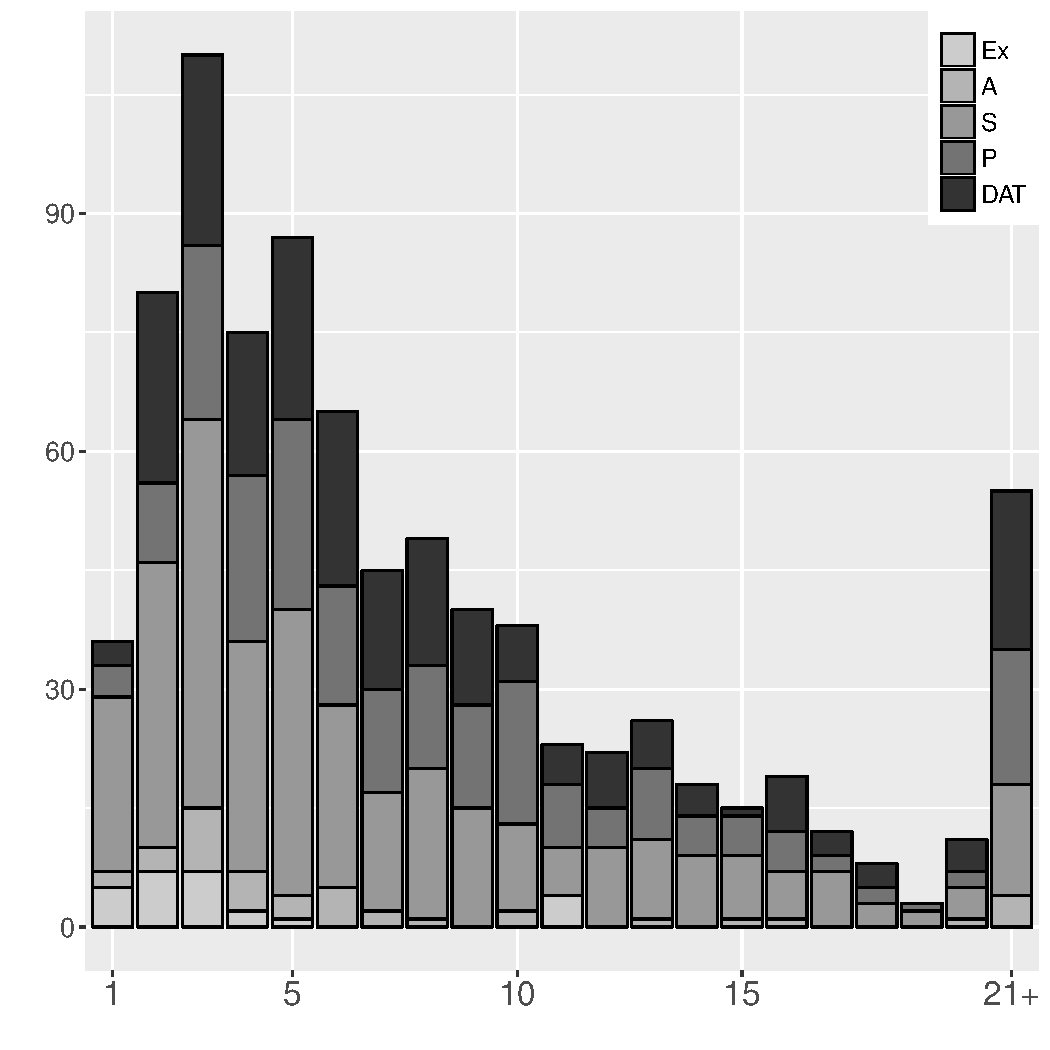
\includegraphics[width=0.95\textwidth]{figure/WOASPPer.pdf}
%	\caption{Word order vs.\ grammatical function (persistent)}
%	\label{WOASPPerF}
%	\end{center}
%\end{minipage}
%\begin{minipage}{0.5\textwidth}
%	\begin{center}
%	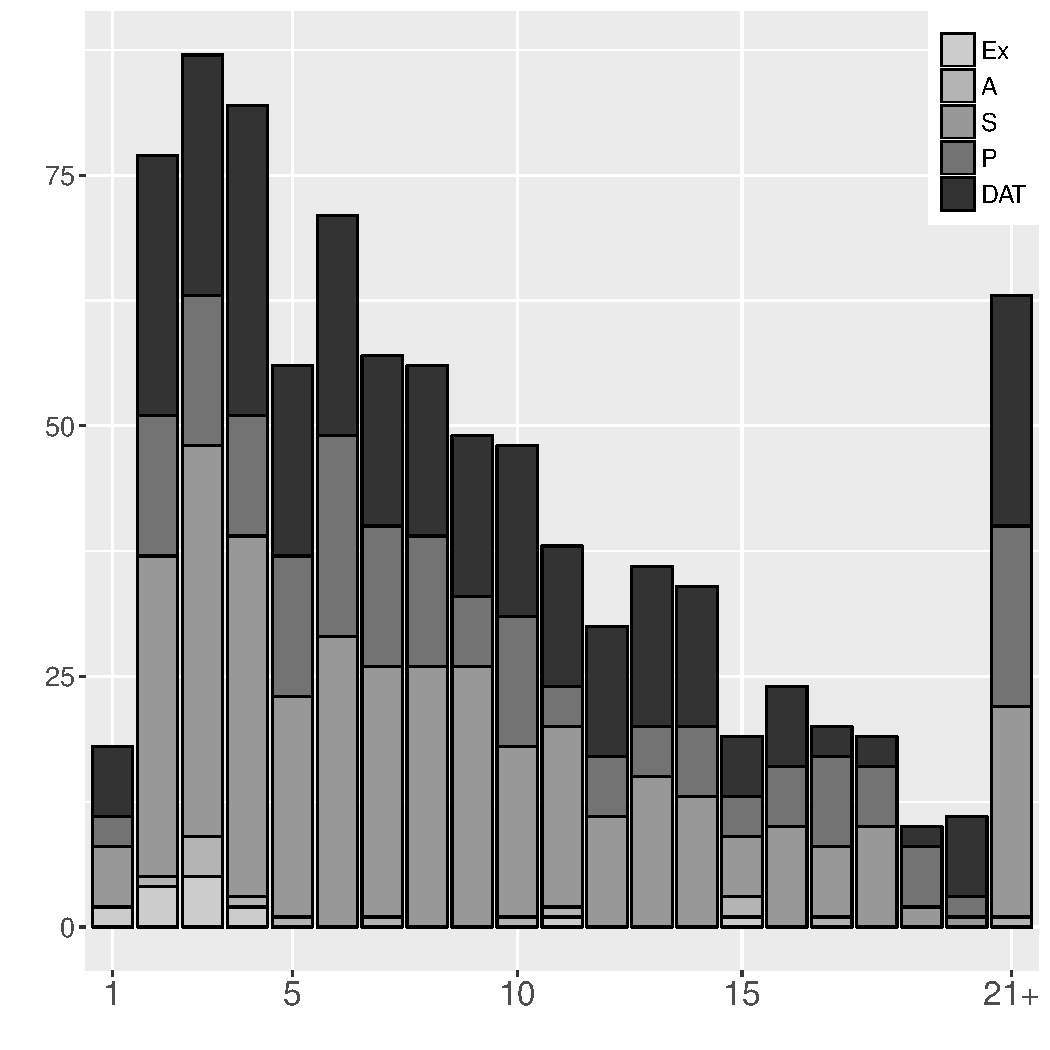
\includegraphics[width=0.95\textwidth]{figure/WOASPNPer.pdf}
%	\caption{Word order vs.\ grammatical function (non-persistent)}
%	\label{WOASPNPerF}
%	\end{center}
%\end{minipage}
%\end{figure}
The following are examples of persistent elements appearing clause-initially.
In \Next,
\ci{hihu-byoo} `skin-disease' in line a, coded by the \isi{topic} marker \ci{toiuno-wa},
appear clause-initially.
The predicate appears in line c,
separated from the subject by a proposition in line b and also another argument (\ci{hito-ni} `person-by') of the clause.
Also in line d, \ci{kore-wa} `this-\ci{wa}', referring to `skin-disease', appears clause initially.
%
\ex.
 \ag. \EM{hihu-byoo-toiuno-wa} \\
 		skin-disease-\ci{toiuno-wa} \\
		`The skin disease,'
 \bg. damat-tei-temo \\
 		keep.silent-\ab{prog}-even.if \\
		`even if you don't tell people about it,'
 \bg. hito-ni \ul{mir-are-te-simau} mono-dat-ta-node \\
 		person-by see-\ab{pass}-and-\ab{pfv} thing-\ab{cop}-\ab{past}-because \\
		`people can see it, so'
 \bg. \EM{kore-wa} ano omot-ta izyooni seesintekini \ul{kutuu-desi}-ta \\
 		this-\ci{wa} \ab{fl} think-\ab{past} more mentally painful-\ab{cop}-\ab{past} \\
		`this was mentally painful more than I had expected.'
		\hfill{(\code{S02F0100: 222.75-231.09})}
%S02F0100|00222751L|222.750605|231.088045|L|皮膚病というのは(0.428)黙っていても(0.285)人に見られてしまうものだったので(0.429)これは(F あの)思った以上に精神的に苦痛でした|[文末]|

Similarly, in \Next,
\ci{sore-wa} `that-\ci{wa}' in line b and g,
and \ci{sore-dake-wa} `that-only-\ci{wa}' in line i,
all of which refer to `chelow kebab' in line a,
appears clause-initially.
%
\ex.
 \a. There is a dish called \EM{chelow kebab}.
 \bg. de \EM{sore-wa} eeto gohan-ni eeto bataa-o maze-te \\
 	and that-\ci{wa} \ab{fl} rice-to \ab{fl} butter-\ci{o} mix-and \\
	`That, you mix rice with butter...'
 \b. on top of that you put spice,
 \b. on top of that you put mutton,
 \b. you mix it and eat it.
 \b. There were many dishes of this kind.
 \bg. \EM{sore-wa} kekkoo sonnani hituzi-no oniku-no kusasa-mo naku-te \\
 	that-\ci{wa} to.some.extent not.really sheep-\ab{gen} meat-\ab{gen} smell-also not.exist-and \\
	`It did not have smell of mutton...'
 \b. I thought it was delicious.
 \bg. \EM{sore-dake-wa} anoo iran-ryoori-no naka-de \ul{taberu} koto-ga ano deki-ta ryoori-desu \\
 		that-only-\ci{wa} \ab{fl} Iran-dish-\ab{gen} inside-\ab{loc} eat thing-\ci{ga} \ab{fl} can-\ab{past} dish-\ab{cop} \\
		`This is the only dish I could eat among \ili{Iranian} dishes.'
 \hfill{(\code{S03F0072: 446.03-447.66})}
%S03F0072|00446026L|446.026013|447.663208|L|チェロカバブというのがありまして|/テ節/|
%S03F0072|00448150L|448.150018|463.667799|L|でそれは(0.114)(F えーと)御飯に(0.376)(F えーと)バターを混ぜてその上に香辛料を振って(0.174)その上に羊のお肉が乗っていて(0.289)それをこう(0.11)混ぜてぐちゃぐちゃに混ぜて食べるという(0.441)(F えーと)お料理が(0.707)(F あのー)(0.681)多かったんですけれども|/並列節ケレドモ/|
%S03F0072|00464361L|464.360734|476.870208|L|それは結構そんなに羊の(0.42)お肉の臭さもなくて(1.094)(F あのー)(0.156)おいしいな(0.178)って(0.418)思ってそれだけは(0.475)(F あのー)イラン料理の中で(0.273)食べることが(0.28)(F あの)できた料理です|[文末]|

\chd{As was mentioned in \ref{WO:Intro},
both \isi{word order} and particles significantly contribute to predict persistence,
contrary to the result of \citeA{imamura17},
who concludes that ``scrambling [PSV order] is pertinent to anaphorically prominent but cataphorically non-prominent objects and that topicalization is especially germane to `continuing \isi{topic}' as the referent of the object'' (p.~78).
There are a few potential reasons for why the results of the present work are different from those of \citeA{imamura17}.
One potential reason is the difference of modalities:
\citeA{imamura17} employed a corpus of written Japanese (\ci{the Balanced Corpus of Contemporary Written Japanese}, BCCWJ), while the present study employs spoken Japanese.
Related to the first point,
clause-chaining, which I will point out is one of the motivations for why clause-initial elements tend to be persistent (see the next section),
only appears in spoken Japanese, but not in written Japanese.
In any case, this is a mere speculation and further studies are needed to analyze
why the results of these two studies differ.}


%%----------------------------------------------------
\subsection{Motivations for topics appearing clause-initially}\label{TopicAppearClause-Initially}

As was pointed out by many linguists,
topics tend to appear clause-initially
because they function as an anchor to the previous \isi{discourse}.
The principle \ref{oldnewprinciple} is motivated by this processing convenience \cite[e.g.,][]{keenan77}.
Clause-initial locatives and other adjectives can also be explained by this motivation.
This anchoring function works best when the \isi{activation cost} of the referent is relatively high \cite{givon83};
i.e.,
when the referent of the element in question is \isi{inferable} or declining.
When the \isi{activation cost} is low, i.e., the \isi{topic} is continuous from the previous \isi{discourse},
the element in question that refers to the \isi{topic} is expected to be zero \cite{givon83,gundeletal93,ariel90};
there is no need for anchoring because the \isi{topic} is already evoked and the \isi{hearer} expects the \isi{topic} to be also mentioned in the current sentence.
This explanation predicts that the distance between the element in question and the \isi{antecedent} is larger when the element in question is expressed in the form of NP instead of zero.
Figure \ref{DistExpTypeF} appears to support this prediction,
\chd{although a statistical analysis indicates that the expression types do not significantly contribute to predict the distance.
This paragraph discusses NPs with long distance.
See the discussion below for NPs with shorter distance.}
The whisker plot in Figure \ref{DistExpTypeF} shows the distance between the element in question (NP vs.\ (explicit) \isi{pronoun} vs.\ zero \isi{pronoun}) and its \isi{antecedent}.
It measures the time between when the \isi{first mora} of the element question is produced and when the \isi{first mora} of the \isi{antecedent} is produced.
The figure shows that the distance between NP and the \isi{antecedent} is larger than that of zero and the \isi{antecedent} in many cases.
Zero pronouns are assumed to be produced at the time
when the \isi{first mora} of the predicate is uttered.

\Next exemplifies this pattern,
\chd{where zero pronouns are indicated by \ci{\O}.}
In line b, \ci{san-nin-me} `the last person' precedes adjuncts (`last fall') and is coded by a variation of \ci{toiuno-wa} (\ci{ttuuno-wa}).
\chd{Zero pronouns \ci{\O} are inserted right before the predicate for the purpose of presentation,
but this does not affect the analysis.}
Since this person is one of the three people mentioned in line a,
this person is \isi{inferable}
through a part-whole relation.
The \isi{topic} moves on to another person in line f, who is also one of the three people mentioned in line a.
In line j, the speaker again refers to the person mentioned in line b.
Also this time, the element \ci{moo hitori-wa} `the other person' appears near clause-initially, preceding other arguments.
The referent continues to be mentioned until line q.
%where the elements that refer to this person is either pronouns, as in line h and k, or zero, as in line i, l, and o.
Finally, the speaker starts talking about himself in line r,
in which case the element \ci{boku-wa} `\ab{1}\ab{sg}-\ci{wa}' appears near clause-initially.
%
\ex.
 \a. All of us three quit this job, interestingly, or strangely.
 \bg. de anoo \EM{san-nin-me-ttuuno-wa} tui se ee kyonen-no o aki-ni yame-ta-n-desu-kedomo \\
 	and \ab{fl} three-\ab{cl}-\ab{ord}-\ci{toiuno}-\ci{wa} just \ab{frg} \ab{fl} last.year-\ab{gen} \ab{fl} fall-in quit-\ab{past}-\ab{nmlz}-\ab{cop}.\ab{plt}-though \\
	`The last person quit this fall.'
 \bg. \EM{soitu-wa} maa itiban saisyo-ni yame-tai yame-tai ttut-ta ningen-nan-desu-kedomo \\
 		\ab{3}\ab{sg}-\ci{wa} \ab{fl} most first-in quit-want quit-want \ab{quot}.say-\ab{past} person-\ab{nmlz}-\ab{cop}.\ab{plt}-though \\
		`He was the first person who said he wanted to quit.'
 \b. This kind of thing often happens.
 \b. All of us three quit eventually.
 \bg. ndee \ul{hitori-wa}-desu-ne \\
 		then one.person-\ci{wa}-\ab{cop}.\ab{plt}-\ab{fp} \\
		`Concerning another person,'
 \b. I guess this is closely related to the fact that we worked in Mobara.
 \bg. de hitotu \ul{sono} \ul{hito-wa} ee ma yappari tonikaku hatarai-te okane-ga koo te-ni \EM{\O} hairu-tte iu koto-ni itiban-no kati-o miidasi-ta wake-desu-ne sono ziki-ni \\
 		then one.thing that person-\ci{wa} \ab{fl} \ab{fl} as.expected any.way work-and money-\ci{ga} this.way hand-to {\O} get.in-\ab{quot} say thing-to most-\ab{gen} value-\ci{o} find-\ab{past} reason-\ab{cop}.\ab{plt}-\ab{fp} that time-at \\
		`At that time this person found it most valuable to work hard and gain money.'
 \b. (Explanation about his view on working. 9.3 sec.)
 \bg. de moo \EM{hitori-wa} maa \EM{kare-mo} hi hizyooni mobara-o aisi-teru-n-desu-ga \\
 	then more one.person-\ci{wa} \ab{fl} \ab{3}\ab{sg}.\ab{m}-also \ab{frg} very Mobara-\ci{o} love-\ab{prog}-\ab{nmlz}-\ab{cop}.\ab{plt}-though \\
	`The other one, who also loves Mobara (a place name),'
 \bg. kondo-no sigoto-tte atarasiku \EM{\O} tui-ta sigoto-tteiuno-wa \\
 		next-\ab{gen} job-\ab{quot} newly {\O} acquire-\ab{past} job-\ci{toiuno}-\ci{wa} \\
		`(his) next job, the new job (he) acquired is...'
 \bg. maa inaka-no hoo-no sigoto-nan-desu-ne \\
 	\ab{fl} rural-\ab{gen} area-\ab{gen} job-\ab{nmlz}-\ab{cop}.\ab{plt}-\ab{fp} \\
	`in rural area.'
 \bg. de \EM{kare} iwaku-desu-ne \\
 	then \ab{3}\ab{sg}.\ab{m} say-\ab{plt}-\ab{fp} \\
	`According to what he says,'
 \bg. sono yama-ga nai tokoro-ni-wa \EM{\O} sum-e-nai-to \\
 	\ab{fl} mountain-\ci{ga} not.exist place-at-\ci{wa} {\O} live-can-\ab{neg}-\ab{quot} \\
 	`He says that he cannot live in places without mountains.'
 \b. Though Mobara does not have mountains, the sky in Mobara is clear.
 \b. We call it Mobara sky. Mobara has such an idyllic scene.
 \bg. sore-ga maa doositemo nai-to \EM{\O} sum-e-nai-tte iu koto-o sono ziki-ni \EM{\O} sato-ta-n-zya-nai-ka-to \\
 	that-\ci{ga} \ab{fl} by.all.means not.exist-\ab{cond} {\O} live-can-\ab{neg}-\ab{quot} say thing-\ci{o} that time-in {\O} learn-\ab{past}-\ab{nmlz}-\ab{cop}-\ab{neg}-\ab{q}-\ab{quot} \\
	`(He) learned at that time that (he) can't live without such scene (I guess).'
 \b. de \EMi{boku-wa}-to ii-masu-to \\
 	then \ab{1}\ab{sg}-\ab{quot} say-\ab{plt}-\ab{cond} \\
	`Talking about myself...'
 \b. ...
   \hfill{(\code{S05M1236: 639.40-738.22})}
%S05M1236|00639399L|639.399427|647.222898|L|て(0.466)(F まー)これがまた(?)(0.115)(F あのー)(0.273)不思議なことにと言うか(0.211)<咳>面白いことにその三人共ですねその会社を(0.187)(F えー)(0.378)辞めました|[文末]|
%S05M1236|00647283L|647.283|653.466794|L|<笑>で(0.587)(F あのー)三人目っつうのはつい(D せ)(F えー)去年の(0.222)(D (? お))秋に辞めたんですけども|/並列節ケドモ/|
%S05M1236|00653467L|653.466794|656.353546|L|そいつは(F まー)一番最初に辞めたい辞めたいっつった人間なんですけども|/並列節ケドモ/|
%S05M1236|00656478L|656.47798|657.577155|L|えてしてそういうもんですが|/並列節ガ/|
%S05M1236|00658101L|658.101232|660.387564|L|(F えー)(0.742)三人共辞めました|[文末]|
%S05M1236|00660711L|660.710985|667.679344|L|んで一人はですね(0.671)(F えー)(0.238)(F ま)これやっぱり茂原で働いたっていうことに大きく関係してそうなんですねその辞めた理由っていうのが||倒置−つなぎ切り
%S05M1236|00667930L|667.930126|678.94475|L|で一つ(D い)その人は(0.608)(F えー)(0.293)(F ま)やっぱり(0.376)とにかく(0.172)働いてお金がこう手に入るっていうことに(0.215)一番の価値観を(0.47)見出だした訳ですねその(0.157)その(D 時)(F えー)時期に||倒置−つなぎ切り
%S05M1236|00679812L|679.811821|689.132829|L|それで今でもですね(0.563)(F まー)(0.166)一番お金が(0.132)入るところっていうんで(0.267)色々職を転々として(0.54)(F まー)(0.294)相当金持ちに(0.284)なってるようですけども|/並列節ケドモ/|
%S05M1236|00689447L|689.446897|694.030141|L|(F まー)一つの生き方かなと(0.427)いう風に(0.372)(F えー)(0.685)僕なんかも見てますけども|/並列節ケドモ/|
%S05M1236|00694880L|694.880285|707.26424|L|でもう一人は(0.959)(F まー)(0.656)彼も(D (? ひ))非常に茂原を愛してるんですが(0.285)(F えー)(0.466)(F ま)今度の仕事っていうのは(0.473)(F あのー)(0.294)今度の仕事って新しく就いた仕事っていうのは(0.39)(F まー)田舎の方(D2 で)(0.275)(F えー)の仕事なんですね|[文末]|
%S05M1236|00708165L|708.164927|711.5187|L|で彼曰くですね(0.192)(F その)山がないところには住めないと|[と文末]|
%S05M1236|00711927L|711.927|728.390145|L|<笑>で茂原ってのは(F まー)山がある訳じゃないんだけど(0.393)(F あのー)(0.308)非常に澄み切った(0.517)(F えー)空でそれのことを(0.24)(F あのー)僕ら茂原晴れと言ってるんですけども(0.602)(F えー)(F まー)(D 非)非常に(F あのー)(0.697)(F まー)(0.215)そういう(0.561)のどかな風景がある訳ですね|[文末]|
%S05M1236|00729305L|729.305466|734.964084|L|で(0.259)<咳>(0.75)それが(F まー)どうしてもないと住めないっていうことをその時期に悟ったんじゃないかと|[と文末]|
%S05M1236|00736425L|736.425057|738.218691|L|で(0.664)僕はと言いますと|/条件節ト/|
%S05M

In this type of example,
clause-initial elements, especially those coded by \isi{topic} markers, function as an anchor to the previous \isi{discourse}.

\begin{figure}
%\begin{minipage}{0.5\textwidth}
	\begin{center}
	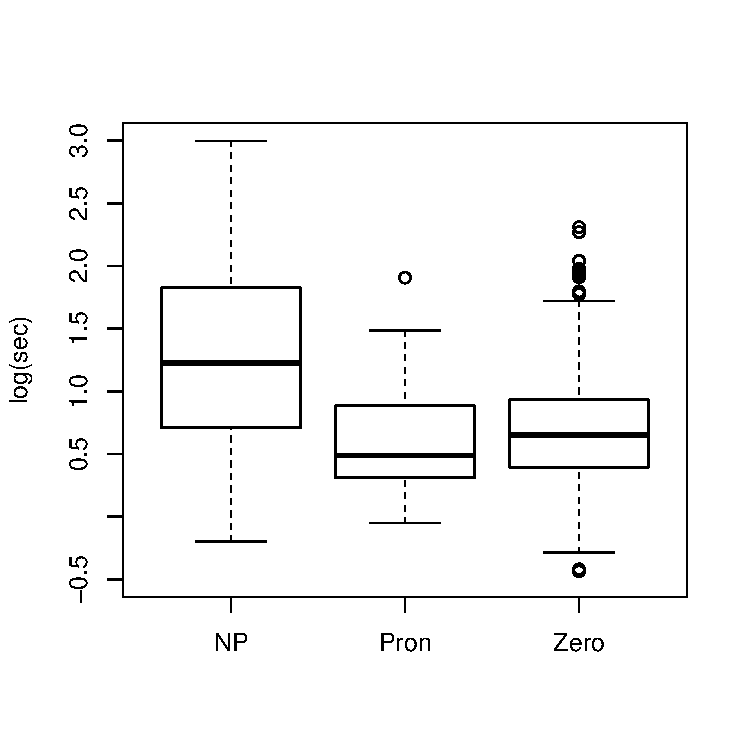
\includegraphics[width=0.5\textwidth]{figure/DistExpType.pdf}
	\caption{Anaphoric distance vs.\ expression type}
	\label{DistExpTypeF}
	\end{center}
%\end{minipage}
\end{figure}


However,
Figure \ref{DistExpTypeF} also indicates that
(explicit) pronouns (\ci{kore} `\ab{dem}.\ab{prox} (this)', \ci{sore} `\ab{dem}.\ab{med} (this/that)', \ci{are} `\ab{dem}.\ab{dist} (that)', \ci{kare} `\ab{3}\ab{sg}.\ab{m} (he)', \ci{kanozyo} `\ab{3}\ab{sg}.\ab{f} (she)')%
	\footnote{
	\ci{Kare} `\ab{3}\ab{sg}.\ab{m} (he)' and \ci{kanozyo} `\ab{3}\ab{sg}.\ab{f} (she)' are very rare in spoken Japanese.
	Instead, \ci{kono hito} `this person' or similar expressions are used more frequently.
	However, this study does not count them as pronouns.
	}
and zero pronouns do not differ from each other.
%Or pronouns even seem to have shorter distance than zeros.
Moreover, there are NPs which refer to the immediate \isi{antecedent}.
\chd{Whereas more than half of the NPs have longer distance than explicit and zero pronouns,
the figure also shows that many NPs have distances as short as those of explicit and zero pronouns.
In fact, a fixed effects analysis for the distance (the expression type as a fixed effect and the speaker as a random effect) indicates that expression types are not a significant factor to predict the distance.}
For example, in the previous example \Last,
the referent of \ci{hitori} `one person' in line f is mentioned in line h as \ci{sono hito} `that person' again,
although the distance is not very far.%
	\footnote{
	The impression of line g is inserted clause rather than \isi{topic} shift.
	}
In a similar manner,
the referent of \ci{san-nin-me} in line b is mentioned in the immediately following clause (line c) as \ci{soitu} `\ab{3}\ab{sg}'.
These examples are not mere exceptions.
In fact, 74.1\% of secondly mentioned referents are still expressed in the form of an NP;
only 21.4\% are expressed as zero and 4.6\% as \isi{pronoun},
as shown in Table \ref{AnaCountExpTypeT} and Figure \ref{AnaCountExpTypeF}.
Figure \ref{AnaCountExpTypeF} and Table \ref{AnaCountExpTypeT} show
the expression type of the element in question based on how many times the referent is mentioned.
"2" indicates that the element in question is mentioned second,
"3" indicates that it is mentioned third, and so on.
The ratio of zero increases as the referent keeps being mentioned.
The fact that the referent introduced is mentioned repeatedly is also reported in \citeA{clancy80}, who investigates Pear Stories;
this pattern is not unique to the corpus of the current study.
\Next is another example
of two NPs which refer to the same referent adjacent with each other.
In this example,
the very long word \ci{yuugosurabia-syakaisyugi-kyoowakoku} `Socialist Federal Republic of Yugoslavia' is repeated twice.
%
\ex.\label{WO:TopicAppearClause-Initially:Ex:Yuugo}
 \ag. ee kon ma kono tiiki ee yu ma \EM{kyuu-yuugosurabia-syakaisyugi-kyoowakoku}-toiu tokoro-nan-desu-keredomo \\
 	\ab{fl} \ab{frg} \ab{fl} this area \ab{fl} \ab{frg} \ab{fl} former-Yugoslavia-socialist-republic-\ab{quot} place-\ab{nmlz}-\ab{cop}.\ab{plt}-though \\
	`This area is called Socialist Federal Republic of Yugoslavia,'
 \bg. kono \EM{yuugosurabia-syakaisyugi-kyoowakoku}-tteiuno-wa motomotoga ee minzoku-tairitu-no hagesii tiiki-de-gozai-masi-te \\
 	this Yugoslavia-socialist-republic-\ci{toiuno}-\ci{wa} originally \ab{fl} ethnic-conflict-\ab{gen} severe area-\ab{cop}-\ab{plt}-\ab{plt}-and \\
	`this Socialist Federal Republic of Yugoslavia is an area with severe ethnic conflicts...'
	\src{S00M0199: 81.95-94.42}
%S00M0199|00081950L|81.949813|94.424971|L|(F えー)(0.143)(D こん)(F ま)この地域(F えー)(D ユ)(0.253)(F ま)旧ユーゴスラビア社会主義共和国というところなんですけれども(0.426)このユーゴスラビア社会主義共和国っていうのは元々が(0.26)(F えー)民族対立の激しい地域でございまして|/テ節/|
%S00M0199|00094875L|94.874776|96.351778|L|(F えー)(0.217)(F ま)一つの||言いさし−言い直しあり
%S00M0199|00096450L|96.449668|124.995828|L|(F えー)(F え)戦後(F えー)第二次大戦終了後(0.115)(F おー)から言われてた言葉として(0.418)(F えー)(D ひ)一つの(0.152)(F えー)(D す)(F ま)政党ですね共産党が支配する(0.418)(F えー)二つの(0.152)(F えー)(F ま)二つの(0.108)(F え)言葉(F え)(F う)(0.196)文字を持ち(0.438)三つの宗教があり(0.219)(F えー)四つの(0.132)(F えー)言語を話す(0.471)で五つの(F えー)民族によって構成される(0.434)国と言われる(F まー)(0.447)(F えー)歴史的に見ても類い稀な(F あ)(F えー)モザイク国家と(0.282)いうことだったんですが|/並列節ガ/|

Why does the speaker repeat the same referent adjacent with each other,
although s/he can fairly assume that the referent has been already evoked by the first mention?
In fact, the second `Socialist Federal Republic of Yugoslavia' in line b cannot be omitted contrary to what is claimed about the nominal forms \cite{givon83,gundeletal93,ariel90}.
Why?

\begin{table}
	\centering
	\tblcaption{Nth mention vs.\ expression type}
	\begin{tabular}{lrrrrr}
	\toprule
          &  2  & 3   &  4 & 5  & 6+ \\
    \midrule
  NP      & 260 & 135 & 83 & 54 & 255 \\
          & \rt{(74.1\%)} & \rt{(64.9\%)} & \rt{(58.0\%)} & \rt{(52.4\%)} & \rt{(40.5\%)} \\
  Pronoun & 16  & 14  & 9  & 13 & 20 \\
          & \rt{(4.6\%)} & \rt{(6.7\%)} & \rt{(6.3\%)} & \rt{(12.6\%)} & \rt{(3.2\%)} \\
  Zero    & 75  & 59  & 51 & 36 & 355 \\
          & \rt{(21.4\%)} & \rt{(28.4\%)} & \rt{(35.7\%)} & \rt{(35.0\%)} & \rt{(56.3\%)} \\
    \midrule
  Sum     & 351 & 208 & 143 & 103 & 630 \\
%          & \rt{(100\%)} & \rt{(100\%)} & \rt{(100\%)} & \rt{(100\%)} & \rt{(100\%)} \\
    \bottomrule
	\end{tabular}
	\label{AnaCountExpTypeT}
%\end{table}
%         2   3   4   5  6+
%  NP   260 135  83  54 255
%  Pron  16  14   9  13  20
%  Zero  75  59  51  36 335
\end{table}

\begin{figure}
	\centering
	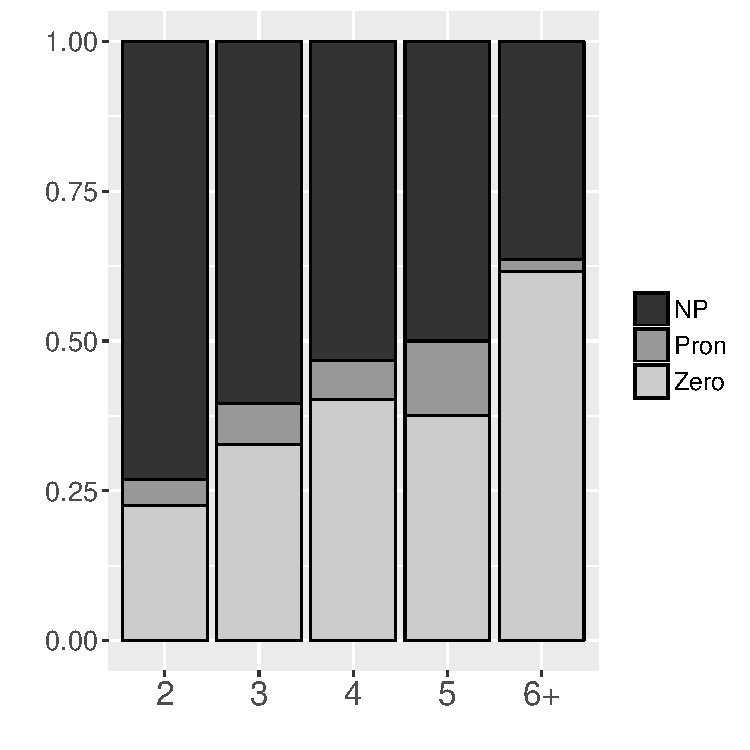
\includegraphics[width=0.5\textwidth]{figure/AnaCountExpType.pdf}
	\caption{Nth mention vs.~expression type}
	\label{AnaCountExpTypeF}
\end{figure}

Since the most frequent \isi{pronoun} in Japanese is the zero \isi{pronoun} as indicated in Figure \ref{AnaCountExpTypeF} and Table \ref{AnaCountExpTypeT},
the speaker needs to make sure that the \isi{hearer} understand which referent zero pronouns refer to.
Therefore, the speaker needs to establish the referent as a \isi{topic}
before s/he uses zero.%
 \footnote{\chd{
 As pointed out by one of the reviewers (Morimoto),
 it is possible to replace `this Socialist Federal Republic of Yugoslavia' in line b of \ref{WO:TopicAppearClause-Initially:Ex:Yuugo} with a pronoun-like form such as \ci{kono kuni} `this country'.
 My argument here still holds because the pronoun-like form `this country' is
 much more informative than the zero \isi{pronoun}.
 The following argument by \citeA{lambrecht94} also suggests that
 focus can be the \isi{antecedent} of overt pronouns, but not zero pronouns.
 See examples \ref{WO:TopicAppearClause-Initially:Ex:John} and \ref{WO:TopicAppearClause-Initially:Ex:Rosa}.
 }}
This might be related to the observation in \citeA[136]{lambrecht94} that
focus elements cannot be the \isi{antecedent} of zero,
while \isi{topic} elements can.
Compare \Next and \NNext (the acceptability judgements are based on Lambrecht. Information structure is added by the present author).
In \Next, \ci{John} is interpreted as \isi{topic} (by default) in \Next[b],
in which case zero is acceptable.
%
\ex.\label{WO:TopicAppearClause-Initially:Ex:John}
 \a. John married Rosa, but he didn't really love her.
 \b. [John]$_{T}$ [married Rosa]$_{F}$, but {\O} didn't really love her.

On the other hand,
in \Next,
\ci{John} is focus because it is the answer to the question,
in which case zero is not acceptable as in \Next[b].
Only an explicit \isi{pronoun} is acceptable, as shown in \Next[a].
%
\ex.\label{WO:TopicAppearClause-Initially:Ex:Rosa}
 \a.[Q:] Who married Rosa?
 \b.[A:]
   \a.[a.] John married Rosa, but he didn't really love her.
   \b.[b.] *?[John]$_{F}$ [married Rosa]$_{T}$, but {\O} didn't really love her.


\begin{figure}
%\begin{minipage}{0.5\textwidth}
	\begin{center}
	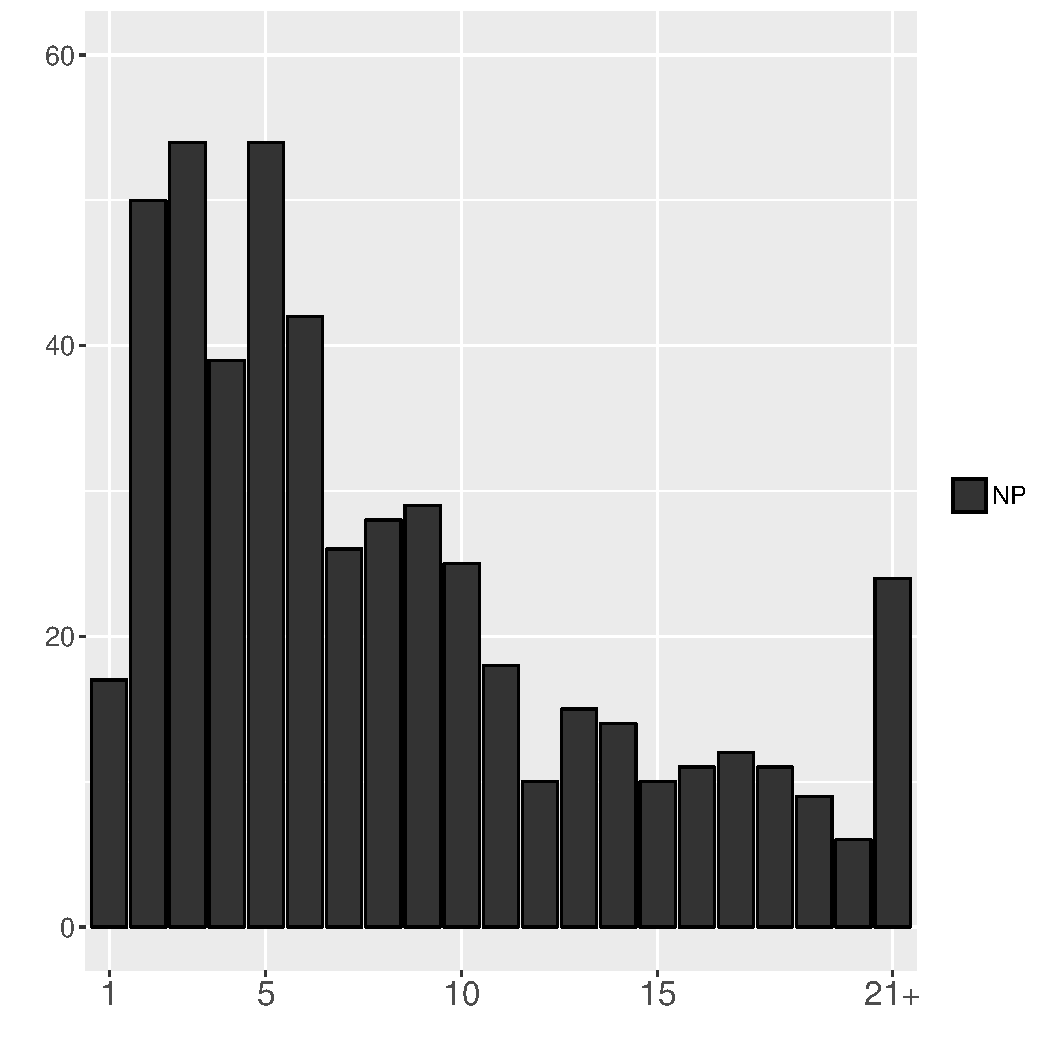
\includegraphics[width=0.6\textwidth]{figure/ExpTypePrevWO.pdf}
	\caption{Antecedent's word order of NPs}
	\label{ExpTypePrevWOF}
	\end{center}
%\end{minipage}
\end{figure}
\begin{figure}
%\begin{minipage}{0.5\textwidth}
	\begin{center}
	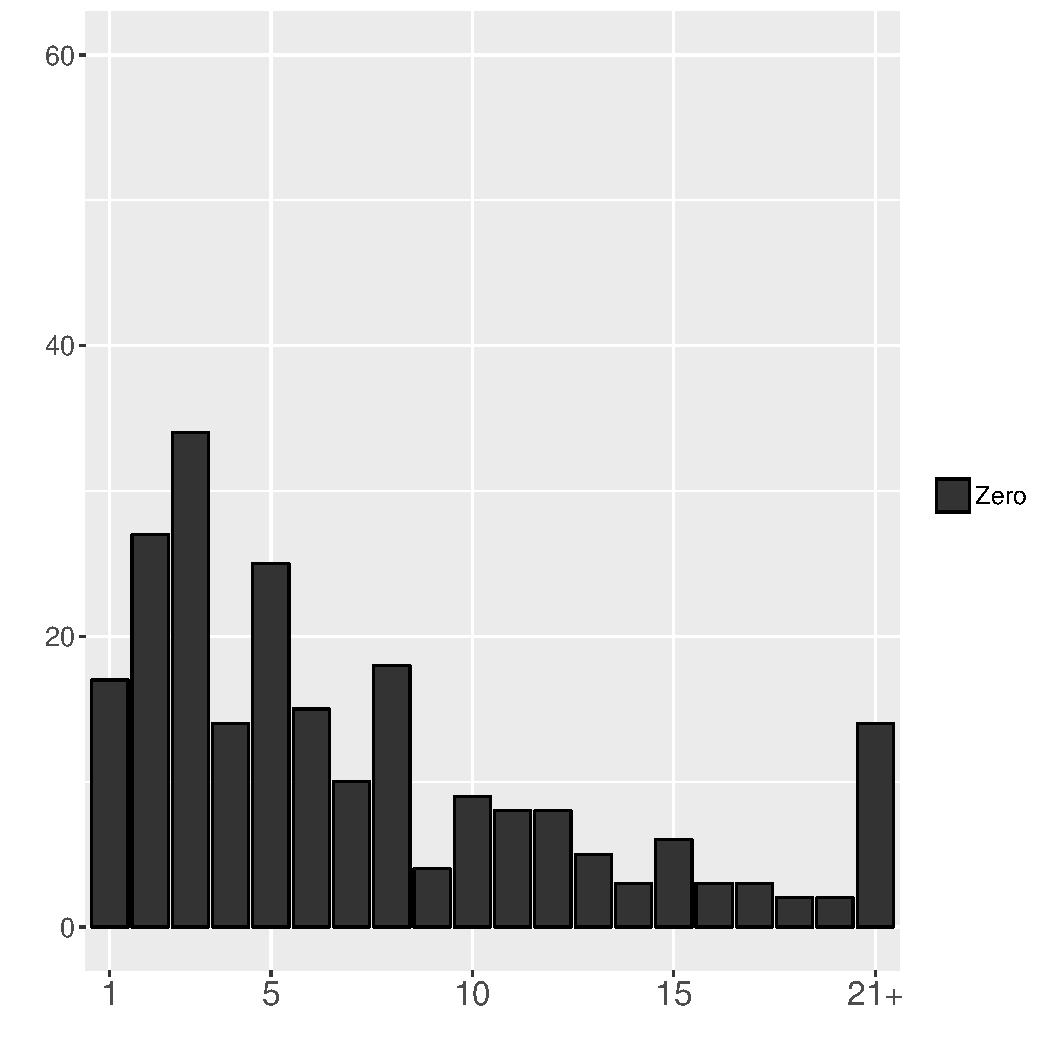
\includegraphics[width=0.6\textwidth]{figure/ExpTypePrevWOZero.pdf}
	\caption{Antecedent's word order of zero pronoun}
	\label{ExpTypePrevWOZeroF}
	\end{center}
%\end{minipage}
\end{figure}

Why do these pronouns or NPs which refer to the immediate \isi{antecedent} appear (near) clause-initially?
I argue that, in addition to the from-old-to-new principle \ref{oldnewprinciple},
the persistent-element-first principle works in \isi{spontaneous speech}.
%
\ex. \label{PerFirstPrinciple}\tl{Persistent-element-first principle}:
 In languages in which \isi{word order} is relatively free,
 the unmarked \isi{word order} of constituents is persistent element first and non-persistent element last.

\chd{One of the factors which motivate this principle is  clause-chaining.
In spoken Japanese, a chain of clauses is frequently observed as schematized in \Next,
where the speaker announces the \isi{topic} at the beginning and continues to talk about it by a chain of multiple clauses.%
 \footnote{
 This is also pointed by Michinori Shimoji (p.c.) on \ili{Ryukyuan} Languages,
 which belong to the same language family as Japanese.
 }
}
%
\ex.
 \a. \fbox{Topic}
 \b. \fbox{Clause1}
 \b. \fbox{Clause2}
 \b. \fbox{Clause3}
 \b. ...

A specific example of clause-chaining is shown in \Next,
where the \isi{topic} `Everest Trail' in line a is preannounced,
and the following clauses (b--f) are about this \isi{topic} `Everest Trail'.
%
\ex.
\ag. \EM{kono} \EM{eberesuto-kaidoo-toiuno-wa} \\
	this Everest-trail-\ab{quot}-\ci{wa} \\
	`{This Everest Trail} is'
\bg. tibetto-to nepaaru-no kooeki-ro-ni-mo nat-te ori-masi-te \\
	Tibet-\ab{com} Nepal-\ab{gen} trade-road-\ab{dat}-also become-and \ab{prog}-\ab{plt}-and \\
	`also used for trading  between Tibet and Nepal.'
\cg. ma zissai-wa nihon-de iu-to \tp{\dvline} \\
	\ab{fl} actual-\ci{wa} Japan-\ab{loc} say-\ab{cond} \\
	`Say, in Japan for example,'
\dg. \EM{\O} takao-san-mitaina yama-miti-nan-desu-keredomo \\
	{\O} Takao-mountain-like mountain-road-\ab{nmlz}-\ab{cop}.\ab{plt}-though \\
	`it's like a road in Mt.\ Takao or something.'
\eg. genti-no hito$\sim$bito-nitotte-wa ee \EM{\O} tuusyoo-ro-to iu-yoona \\
	local-\ab{gen} person$\sim$\ab{pl}-for-\ci{wa} \ab{fl} {\O} trade-road-\ab{quot} say-like \\
\bg. insyoo-no \EM{\O} miti-desi-ta \\
	 impression-\ab{gen} {\O} road-\ab{cop}.\ab{plt}-\ab{past} \\
 `{it} was a road like a trading road for local people.'
 \b.[] \hfill{(\code{S01F0151: 105.73-120.14})}
%このエベレスト街道というのは
%チベットとネパールの交易路にもなっておりまして
%ま実際は日本で言うと
%高尾山みたいな山道なんですけれども
%現地の人々にとってはえー通商路というような印象の道でした (S01F0151: 105.73-120.14)

\chd{This pattern is useful because which referent the speaker talks about in the chain of clauses in question is referred to at the beginning of the chain and s/he can use the zero \isi{pronoun} in the following clauses.}

%This principle is motivated by processing;
%it is easier for the \isi{hearer} to process if the \isi{topic} to be talked about is stated first.
%It is easy also for the speaker to say the \isi{topic} first
%because s/he has already activated the \isi{topic} to be talked about,
%but not necessarily how to express the following content.
%	\footnote{
%	This might be the same as the from-old-to-new principle (\ref{oldnewprinciple}).
%	}
Figure \ref{ExpTypePrevWOF} and \ref{ExpTypePrevWOZeroF} show the \isi{word order} of antecedents of NPs and zero pronouns, respectively.
Although the contrast is subtle,
the antecedents of zero pronouns are more skewed towards earlier positions than NPs.
%The figure is a bar plot of expression types of elements based on the word orders of their antecedents.
%The x-axis indicates the \isi{word order} of the antecedents and y-axis indicates the raw frequencies of elements.

Consider the following example \Next.
The speaker mentions the \isi{topic} `the participants of the trekking' first in line a,
and describes this in the following \isi{discourse}.
After \Next[f],
the speaker extends the \isi{topic} and describes each participant.
%
\ex.\label{trekking}
 \ag. e \EM{torekking-sankasya}-nituki-masite-wa \\
 	\ab{fl} trekking-participant-about-\ab{plt}-\ci{wa} \\
	`Concerning the participants of this trekking,'
 \bg. moo hontooni ni-zyuu-go-sai-no ooeru-san-kara \\
 	\ab{fl} really two-ten-five-years.old-\ab{gen} working.woman-\ab{hon}-from \\
	`from the 25-year-old working lady,'
 \bg. nana-zyuu-ni-sai-no ozii-san-made \\
 	seven-ten-two-years.old-\ab{gen} old.guy-\ab{hon}-till \\
	`to the 72-year-old elderly man,'
 \bg. hizyooni takusan-no hito$\sim$bito-ga \\
 	very many-\ab{gen} person$\sim$\ab{pl}-\ci{ga} \\
	`many people...'
 \b. no, not many people,
 \bg. ta-syu-ni wataru nenree-soo-no hito-ga i-te omosirokat-ta-desu \\
 		many-kind-\ab{dat} cover age-tier-\ab{gen} person-\ci{ga} exist-and interesting-\ab{past}-\ab{plt} \\
		`there were many kinds of people from a wide age range and it was interesting.'
		\src{S01F0151: 597.67-610.87}
%S01F0151|00597665L|597.665333|610.870275|L|(F え)トレッキング参加者につきましては(0.192)もう本当に二十五歳の(A オーエル;OL)さんから七十二歳のお爺さんまで(0.278)非常にたくさんの人々が(0.539)(F えー)(0.131)<FV>たくさんのじゃない(0.11)多種に渡る(0.237)年齢層の人がいて面白かったです|[文末]|
%S01F0151|00611451L|611.450993|614.022662|L|で(0.429)みんな人によって趣味が違いまして|/テ節/|
%S01F0151|00614377L|614.37677|626.616677|L|登山から(0.325)(F え)登山が趣味の方もいれば写真を撮るのが趣味の方もいて(0.352)後は(D こせ)高山植物に非常に詳しい方もいれば(0.328)バードウォッチングに詳しくて物凄く立派な双眼鏡を持ってくる方もいたりして|<テ節>|直後がまとめ表現
%S01F0151|00626928L|626.928382|634.442324|L|(F ま)私達はっきり言って何も知らないで参加したので全部人に(0.301)あれは何ですかとか言って聞きながら(0.292)教えていただいて(0.317)登っていました|[文末]|

In this kind of example,
clause-initial elements do not refer to zero pronouns as constituents in the following clauses,
but are only pragmatically associated with the constituents in the following clauses (see also \S \ref{Par:Subj:Ex}).


\begin{table}
 \tblcaption{Antecedent's particle vs.~current expression type}
 \label{ExpTypePrevParT}
\begin{tabular}{lrrrr}
 \toprule
          & \ci{toiuno-wa} & \ci{wa} & \ci{ga} & \ci{o} \\
 \midrule
 NP       & 11             & 38      & 80      & 89 \\
          & \rt{(36.7\%)}  & \rt{(46.3\%)} & \rt{(63.0\%)} & \rt{(74.8\%)} \\
 Pronoun  & 4              & 3       & 5       & 3 \\
          & \rt{(13.3\%)}  & \rt{(3.7\%)} & \rt{(3.9\%)} & \rt{(2.5\%)} \\
 Zero     & 15             & 41      & 42      & 27 \\
          & \rt{(50.0\%)}  & \rt{(50.0\%)} & \rt{(33.1\%)} & \rt{(22.7\%)} \\
 \midrule
 Sum      & 30             & 82      & 127     & 119 \\ 
%          & \rt{(100\%)}   & \rt{(100\%)} & \rt{(100\%)} & \rt{(100\%)} \\
 \bottomrule
%           NP Pron Zero
%  toiuno-wa 11    4   15
%  wa        38    3   41
%  ga        80    5   42
%  o         89    3   27
\end{tabular}
\end{table}

\begin{figure}
	\begin{center}
	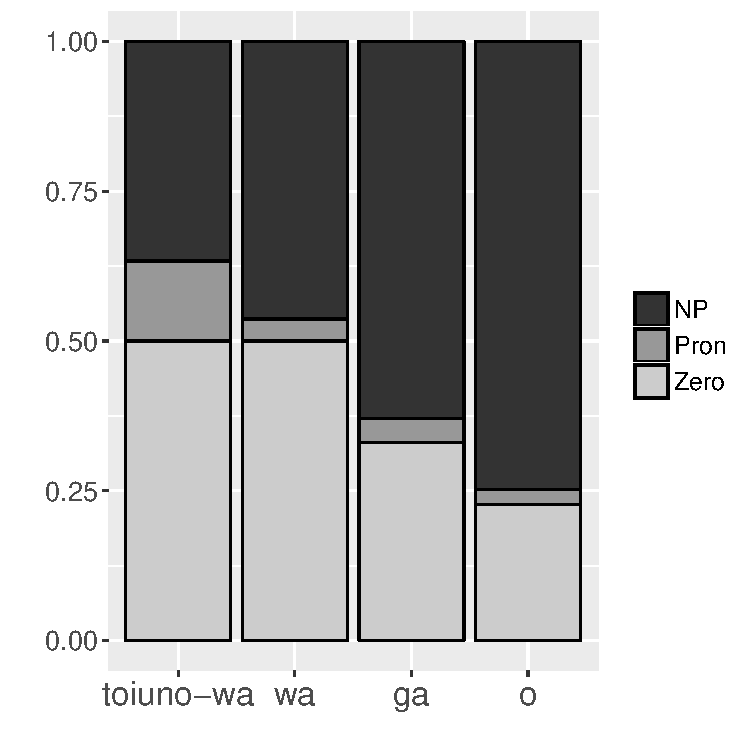
\includegraphics[width=0.5\textwidth]{figure/ExpTypePrevPar.pdf}
	\caption{Antecedent's particle vs.~current expression type}
	\label{ExpTypePrevParF}
	\end{center}
\end{figure}

Not all clause-initial antecedents of zero pronouns are coded by \isi{topic} markers.
Figure \ref{ExpTypePrevParF} is a bar plot of expression types of elements based on the particles of their antecedents.
According to the figure, the antecedents of zero pronouns are more likely to be coded by \ci{wa} or \ci{toiuno-wa} than
those of overt NPs,
although there are many antecedents of zeros coded by \ci{ga} or \ci{o}.

In the following example \Next,
%\ci{syoo-doobutu} `an small animal' in line b is new 
%%
%\ex.
% \a. When we were having dinner,
% \bg. n mado-no tokoro-to iu-ka beranda-ni nanika \EM{syoo-doobutu-ga} koo tyokotyoko-to ki-ta-n-desu-ne \\
% 	\ab{fl} window-\ab{gen} place-\ab{quot} say-\ab{q} balcony-to something small-animal-\ab{nom} this.way \ab{ono}-\ab{quot} come-\ab{past}-\ab{nmlz}-\ab{cop}.\ab{plt}-\ab{fp} \\
%	`a small animal came near the window, or the balcony.'
% \bg. de saisyo koo ano sotira-no soto-no hoo-kara \EM{\O} nozoi-ta mon-desu-kara \\
% 	then at.first this.way \ab{fl} that-\ab{gen} outside-\ab{gen} direction-from {\O} look-\ab{past} thing-\ab{nmlz}.\ab{cop}-because \\
%	`At first, (it) appeared from the outside, that way, so'
% \bg. watasi-wa saisyo \EM{\O} risu-kana-to omot-ta-n-desu \\
% 	\ab{1}\ab{sg}-\ci{wa} at.first {\O} squirrel-\ab{q}-\ab{quot} think-\ab{past}-\ab{nmlz}-\ab{cop}.\ab{plt} \\
%	`at first I thought (it) was a squirrel.'
% \bg. de tu sat-to koo are-to omot-te it-tara sat-to \EM{\O} nige-tyai-masi-te \\
% 	then \ab{frg} \ab{ono}-\ab{quot} this.way \ab{fl}-\ab{quot} think-and go-then \ab{ono}-\ab{quot} {\O} escape-\ab{pfv}-\ab{plt}-and \\
%	`(I) was wondering and approached (the balcony), then (it) ran away.'
%	\src{S00F0014: 612.71-621.50}
%S00F0014|00612711L|612.710582|621.496514|L|それで(0.344)(F あのー)<FV>(0.176)夜に(0.554)(F あの)食事をこうしてましたら(0.748)(F ん)窓のところと言うかベランダに何か小動物がこうちょこちょこと来たんですね|[文末]|
%S00F0014|00621815L|621.814615|627.660077|L|で最初こう(0.282)(F あの)(0.12)そちらの外の方から覗いたもんですから(0.312)私は最初(0.265)リスかなと思ったんです|[文末]|
%S00F0014|00628000L|627.999519|631.707987|L|で(0.329)(D (? つ))さっとこう(F あれ)(0.235)と思って行ったらさっと逃げ(0.169)ちゃいまして|/テ節/|
\ci{waru-gaki} `brats', which is coded by \ci{ga} clause-initially in line a, is the \isi{antecedent} of the zero in line b.
%
\ex.
 \ag. a dokka-no kinzyo-no \EM{waru-gaki-ga} sute-inu-o mi-te \\
		\ab{fl} somewhere-\ab{gen} neighborhood-\ab{gen} bad-brat-\ci{ga} abandon-dog-\ci{o} look-and \\
		`Brats around here found this abandoned dog, and'
 \bg. akai penki-o hana-no ue-ni \EM{\O} nut-ta-n-daroo-to \\
 	red paint-\ci{o} nose-\ab{gen} above-\ab{dat} {\O} paint-\ab{past}-\ab{nmlz}-\ab{infr}-\ab{quot} \\
	`(they) must have painted the dog's nose red.'
 \b. (we) were talking like this.
 \src{S02M0198: 176.26-184.61}
%S02M0198|00176259L|176.258754|184.61063|L|(F あ)どっかの(0.161)近所の悪がきが(0.461)捨て犬を見て(0.599)赤いペンキを(0.263)鼻の上に塗ったんだろうと(0.193)話したんですけども|/並列節ケドモ/|

This might sound \ci{a priori} to some readers because Japanese is traditionally argued to be an SOV language:
of course \ci{ga}-coded elements are subjects and precede other arguments.
However, what I claim is that
the persistent-element-first principle \ref{PerFirstPrinciple}, in addition to the from-old-to-new principle \ref{oldnewprinciple}, is one of the motivations for so-called subjects (A and S) to precede other arguments.
%As \citeA{lambrecht94} points out, topics tend to be outside of a clause, i.e., they do not belong to the arguments of a clause as in \Next.
%In \Next[a],
%the expression \ci{the African elephant} is not an argument of the predicate \ci{fan};
%\ci{fan} has A as \ci{he} and P as \ci{himself}.
%Similarly, in \Next[b],
%\ci{the typical family today} is also non-argument;
%the argument of the \isi{verb} \ci{work} is \ci{the husband and the wife}.
%%
%\ex.
% \a. (Six year old girl, explaining why the African elephant has bigger ears than the Asian elephant)
% 	\EM{The African elephant}, it's so hot there, so he can fan himself.
% \b. (From a TV interview about the availability of child care)
% 	That isn't the typical family anymore.
%	\EM{The typical family today}, the husband and the wife both work.
%	\hfill{\cite[][p.~193 (emphasis added)]{lambrecht94}}
%
%In the same way,
%`the participants of the trekking' in (\ref{trekking}) is not an argument of the clause (\ref{trekking}f).
%The argument of the \isi{verb} \ci{i(ru)} `exist' is \ci{hito} `person'.

Another motivation has been pointed out for \isi{topic} elements immediately repeated clause-initially.
\citeA{dennakagawa13} discuss cases where clause-initial topics are used as fillers.
Since topics have already been evoked in the speaker's mind, the cost of producing topics is lower than that of producing new elements.
While the speaker utters the \isi{topic},
s/he plans the following \isi{utterance}.
\citeA{dennakagawa13} investigated conversations and found that the \isi{topic} elements repeated immediately after the previous speaker's \isi{utterance}
complementarily distribute with fillers.
They also found that the length of the final mora of the \isi{topic} phrase (typically \ci{wa}) correlates with the length of the following \isi{utterance}
\cite[see also][]{watanabeden10}.
%This might be another motivation for topics being outside of a clause.
In the following example \Next,
not only `Serbian people' is repeated twice in line a and b,
the whole sentence is almost repeated;
the sentences in line a and b convey almost the same proposition.
This is another piece of evidence that supports Den \& Nakagawa's claim;
while repeating almost the same proposition,
the speaker can plan what to say next about this \isi{topic}.
%
\ex.
 \ag. sono \EM{serubia-zin-no} \EM{kata-tati}-ga soko-ni-wa ma hazimete ee serubia-teekoku-toiu kokka-o tukuru-no-ga maa zyuu-ni-seeki-no ma owari-gurai-nan-desu-ga \\
 	that Serbia-people-\ab{gen} person.\ab{plt}-\ab{pl}-\ci{ga} there-\ab{dat}-\ci{wa} \ab{fl} first.time \ab{fl} Serbia-empire-\ab{quot} nation-\ci{o} make-\ab{nmlz}-\ci{ga} \ab{fl} ten-two-century-\ab{gen} \ab{fl} end-around-\ab{nmlz}-\ab{cop}.\ab{plt}-though \\
	`Those Serbian people built a nation called the Serbian Empire towards the end of the eleventh century.'
 \bg. ee kono ziki maa \EM{serubia-no} \EM{kata-tati}-ga maa koko-ni tu kokka-o tukut-te ee serubia-teekoku-toiu koto-de \\
 	\ab{fl} this time \ab{fl} Serbia-\ab{gen} person.\ab{plt}-\ci{ga} \ab{fl} here-\ab{dat} \ab{frg} nation-\ci{o} make-and \ab{fl} Serbia-empire-\ab{quot} thing-\ab{cop}.and \\
	`Around this time Serbian people build a nation, this is the Serbian Empire and'
 \bg. ee ryuusee-o \EM{\O} kiwame \\
 		\ab{fl} flourish-\ci{o} {\O} be.extreme \\
	`(it) flourished.'
 \b. At that time Catholics were coming from the north, and from the south, \ili{Greek} Orthodox were coming,
 \b. though they are both Christian,
 \bg. ee ni-keetoo-no syuukyoo-no naka-de seekatu-o \EM{\O} si-te-iku naka-de \\
 		\ab{fl} two-stream-\ab{gen} religion-\ab{gen} inside-\ab{loc} life-\ci{o} {\O} do-and-go inside-\ab{loc} \\
		`While (they) were living surrounded by two streams of religion,'
 \bg. ee serubia-teekoku-tosite ma dotira-o erabu-ka-tteiu na ko ee koto-no naka-de \\
 	\ab{fl} Serbia-empire-as \ab{fl} which-\ci{o} choose-\ab{q}-\ab{quot} \ab{frg} \ab{frg} \ab{fl} thing-\ab{gen} inside-\ab{cop}.and \\
	`(they) faced the question of which one to choose.'
 \bg. ee ma minami-gawa-no girisya-seekyoo-o \EM{\O} toru wake-nan-desu-ga \\
 	\ab{fl} \ab{fl} south-side-\ab{gen} \ili{Greek}-Orthodox-\ci{o} {\O} choose reason-\ab{nmlz}-\ab{cop}.\ab{plt}-though \\
	`(They) eventually chose \ili{Greek} Orthodox.'
	\src{S00M0199: 212.34-221.02}
%S00M0199|00212336L|212.336343|221.023973|L|そのセルビア人の方達がそこには(F ま)初めて(0.163)(F えー)セルビア帝国という(0.373)(F えー)国家を作るのが(F まー)十二世紀の(0.436)(F ま)終わりぐらいなんですが|/並列節ガ/|
%S00M0199|00221455L|221.455248|229.24769|L|(F えー)この時期(F まー)(0.976)セルビアの方達が(F まー)ここに(D つ)国家を作って(0.151)(F えー)セルビア帝国ということで(0.266)(F えー)隆盛を極め|/連用節/|
%S00M0199|00229652L|229.651772|254.15569|L|(F えー)そしてその後(F まー)(F あのー)(F まー)その当時宗教としては(0.337)(F えー)北からは(F えー)(0.13)(D く)(F ま)キリスト教のカトリック(0.128)(F えー)南からは(0.372)(F えー)(F い)ギリシャ正教ということで(F えー)二つの(F えー)(F ま)同じキリスト教ですが(F えー)二系統の宗教の中で(0.327)生活をしていく中で(0.391)(F えー)セルビア(0.177)帝国として(F ま)どちらを選ぶかっていうな(0.212)(D こ)(F えー)ことの(D ん)中で(F えー)(0.14)(F ま)(0.561)南側のギリシャ正教を取る訳なんですが|/並列節ガ/|


%%----------------------------------------------------
\subsection{Summary of clause-initial elements}

This section investigated characteristics of clause-initial elements.
It turned out that
shared and persistent elements tend to appear clause-initially.
Not only did this study confirm the classic observation that
topics tend to appear clause-initially,
this section and the next section analyze what kind of topics appear clause-initially.
I also discussed motivations for clause-initial topics.


%%----------------------------------------------------
%%----------------------------------------------------
\section{Post-predicate elements}\label{WOPostPreEles}

While Japanese is reported to be a \isi{verb-final language} \cite{hinds86,shibatani90},
some elements appear after the \isi{verb} in spoken Japanese \cite{kuno78,onosuzuki92,fujii95,takami95a,takami95b,ono06,nakagawaetal08_paper}.
The following are examples of post-predicate elements.
Since post-predicate elements are very rare in monologues,
the examples are from the dialogue part of CSJ.
\ci{Kono hito} `this person' in \Next and \ci{terii itoo} `Terry Ito (A person's name)' in \NNext are produced after the predicates \ci{yat} `do' and \ci{kake} `wear', respectively.
%
\ex.
\ag.[R:] nani \EMi{yat}-teru-no \EM{kono} \EM{hito} \\
 		what do-\ab{prog}-\ab{nmlz} this person \\
		`What is (he) doing, this person?'
		\src{D02F0028: 193.30-194.45}

\ex.\label{D02F0015_TerryIto}
 \ag.[L:] sangurasu-toka \EMi{kake}-te-masu-yo-ne \EM{terii} \EM{itoo-tte} \\
		sunglasses-\ab{hdg} wear-\ab{prog}-\ab{plt}-\ab{fp}-\ab{fp} Terry Ito-\ab{quot} \\
		`(He) is wearing sunglasses, isn't he, Terry Ito?'
		\src{D02F0015: 359.17-362.42}

This section investigates the \isi{information structure} of post-predicate constructions of this kind.
Although post-predicate expressions could be adverbs, connectives, and other adjuncts,
this study only examines noun phrases.
%I call all the elements which appear before the predicate
%``elements before the predicate'' or ``preposed elements''
%as opposed to ``post-predicate'' or ``postposed'' elements.
%I keep the term ``pre-posed'' elements
%to indicate elements which appear immediately before the predicate
%(to be discussed in \S \ref{WOPrePredEles}).

%%----------------------------------------------------
\subsection{Strongly evoked elements appear after predicate}\label{WORdis}

\citeA[][136]{takami95a} argues that
postposed elements are elements other than the focus.
For example,
the answer to a question or \ci{wh}-phrase cannot be postposed naturally.
\Next is an example of a \isi{postposed element} `a 10-carat diamond ring' as the answer to the question `what'.
While the sentence itself is natural,
the \isi{postposed element} cannot felicitously be the answer to a question.
%
\ex.
 \a.[Q:] What did Taro buy for Hanako?
 \bg.[A:] \#taroo-wa hanako-ni kat-te yat-ta-yo \EM{zyuk-karatto-no} \EM{daiya-no} \EM{yubiwa-o} \\
 		Taro-\ci{wa} Hanako-for buy-and give-\ab{past}-\ab{fp} 10-carat-\ab{gen} diamond-\ab{gen} ring-\ci{o} \\
		`Taro bought (it) for Hanako, a 10-carat diamond ring.'

Similarly,
\ci{wh}-phrases such as \ci{dore} `which' cannot be postposed,
as shown in \Next.
%
\exg. *itiban oisii-desu-ka \EM{dore-ga}? \\
		most delicious-\ab{cop}.\ab{plt}-\ab{q} which-\ci{ga} \\
		`The most delicious one, which?'


%As has been pointed out in \citeA{onosuzuki92,takami95b,ono06,nakagawaetal08_paper},
%topics can be postposed.
\citeA{nakagawaetal08_paper} found that
there are two types of \isi{post-predicate construction}:
the single-contour and the double-contour types.
The single-contour type is a type of \isi{post-predicate construction}
where the post-predicate elements are uttered without a pause and do not have the F$_{0}$ peak,
whereas the double-contour type is a type of construction
where the post-predicate elements are uttered with a pause and do have the F$_{0}$ peak.
The \isi{pitch} contours of each \isi{utterance} are shown in Figure \ref{kome1F} for the single-contour type (\Next[A] and \NNext[A]) and \ref{kome2F} for the double-contour type (\Next[A$^{\prime}$] and \NNext[A$^{\prime}$]),
both of which are produced by the author.
The post-predicate part is \ci{kome-wa} `rice-\ci{wa}',
whose accent nucleus is on \ci{me} and overall accent is supposed to be LHL (L indicates low and H indicates high in \isi{pitch}).
In Figure \ref{kome1F}, where the \isi{postposed element} is uttered with the same continuous contour as the \isi{main clause},
one can neither observe the F$_{0}$ peak in \ci{me} nor a pause between the predicate and the \isi{postposed element}.
In Figure \ref{kome2F}, on the other hand,
where the \isi{postposed element} is uttered in a separate contour from the \isi{main clause},
one can observe the F$_{0}$ peak in \ci{me} and a pause between the predicate and the \isi{postposed element}.

\citeA{nakagawaetal08_paper} investigated the difference between these two types in terms of \isi{information structure} and found that
the post-predicate elements of the single-contour type are evoked
by being mentioned immediately before or through physical context.
On the other hand,
those of the double-contour type are not necessarily evoked.
For example, compare the following examples \Next and \NNext,
where the bold-faced letters indicate that
they are high in \isi{pitch}.%
	\footnote{
	Here I assume that the \isi{pitch accent} of \ci{oisii} `good' is LHHH
	and that of \ci{kome-wa} `rice-\ci{wa}' is LHL.
	}
The referent `rice' in \Next is evoked
because it is mentioned in \Next[Q] immediately before the answer to Q is uttered.
In this case,
\Next[A$^{\prime}$],
where the \isi{post-predicate element} \ci{kome-wa} `rice-\ci{wa}' has its own F$_{0}$ peak and is preceded by a pause,
is not acceptable,
while \Next[A],
where the \isi{post-predicate element} without its own F$_{0}$ peak is uttered immediately after the predicate without a pause,
is acceptable.
%
\ex. \tl{The referent `rice' evoked}
 \a.[Q:] I don't like rice.
	\bg.[A:] o\pk{isii}-yo \ul{kome-wa} \\
			good-\ab{fp} rice-\ci{wa} \\
	\bg.[A$^{\prime}$:] ?o\pk{isii}-yo, \ul{ko\pk{me}-wa} \\
			good-\ab{fp} rice-\ci{wa} \\
			`RICE is good (but others not).'
			\hfill{\cite[][7]{nakagawaetal08_paper}}

On the other hand,
in \Next, where `rice' is not evoked before the speaker utters \Next[A] or \Next[A$^{\prime}$],
only the double-contour type \Next[A$^{\prime}$] is acceptable
and the single-contour type \Next[A] is not natural.
\ex. \tl{The referent `rice' not evoked}
 \a.[Q:] Is that sushi bar good?
	\bg.[A:] ??o\pk{isii}-yo \ul{kome-wa} \\
			good-\ab{fp} rice-\ci{wa} \\
	\bg.[A$^{\prime}$:] o\pk{isii}-yo, \ul{ko\pk{me}-wa} \\
			good-\ab{fp} rice-\ci{wa} \\
			`RICE is good (but others not).'
			\hfill{(ibid.)}

The remaining issue is
to investigate the difference between elements before and after the predicate in terms of \isi{information structure}.

\begin{figure}
%\begin{minipage}{0.5\textwidth}
	\begin{center}
	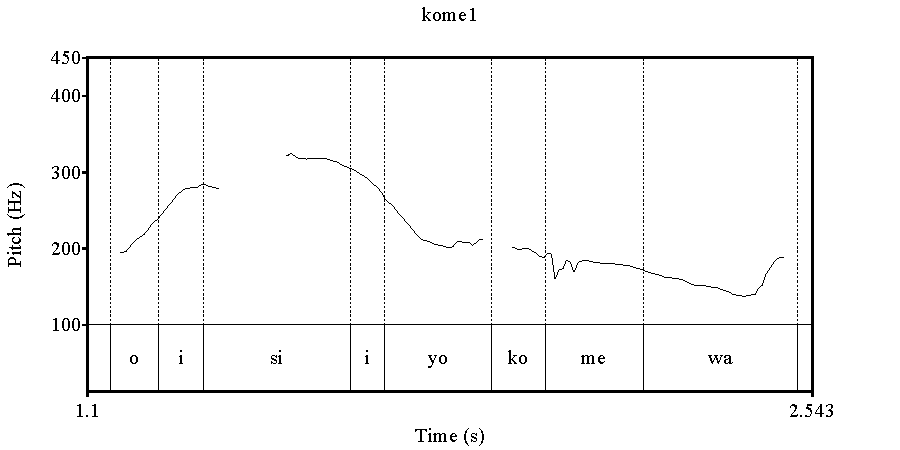
\includegraphics[width=0.6\textwidth]{sounds/kome1.pdf}
	\caption{Post-predicate construction: single-contour type}
	\label{kome1F}
	\end{center}
%\end{minipage}
\end{figure}
\begin{figure}
%\begin{minipage}{0.5\textwidth}
	\begin{center}
	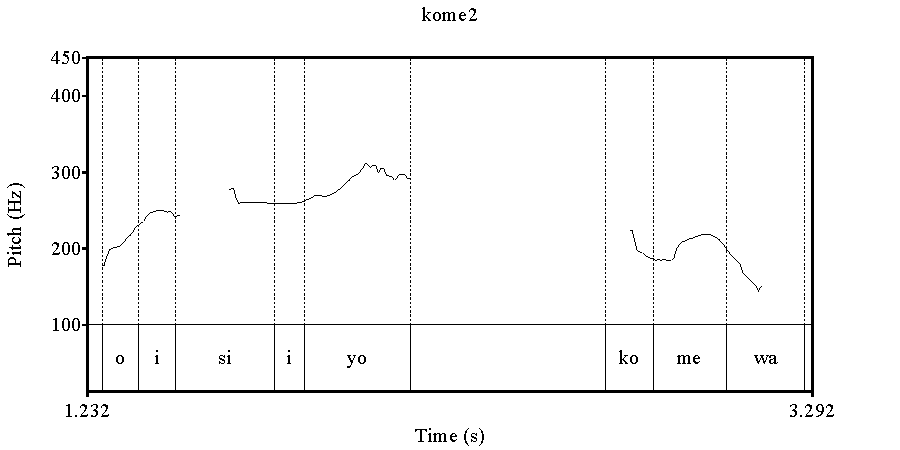
\includegraphics[width=0.6\textwidth]{sounds/kome2.pdf}
	\caption{Post-predicate construction: double-contour type}
	\label{kome2F}
	\end{center}
%\end{minipage}
\end{figure}

\citeA{nakagawaetal08_paper} measured the referential distance (RD) between the post-predicate elements and their antecedents,
i.e., they measured the number of inter-pausal units between the element in question and its \isi{antecedent}.
They modified the definition of RD from the original one \cite{givon83} and decided to use inter-pausal unit as a measure of RD
since clause boundaries are sometimes difficult to identify in spoken Japanese.
Their results are shown in Table \ref{RDPostT}.
The table shows that the average RD of the post-predicate elements of the single-contour type is 6.9 on average,
whereas that of the double-contour type is 39.7.
What about elements before the predicate?

I conducted the same investigation for elements before the predicate, but this time I used monologues employed throughout this study
because the dialogues Nakagawa and her colleagues used in their study lack the information about RD of elements before the predicate.%
	\footnote{
	\citeA{nakagawaetal08_paper} counted the RD of non-\isi{anaphoric} elements as 100 (the maximum value of RD),
	but this study didn't include non-\isi{anaphoric} elements
	since I thought that this is ad hoc.
	This modification makes the RD of elements before the predicate (conducted in this study) smaller.
	This has only a small effect and the overall conclusion does not change because
	according to our result,
	the RD of pre-predicate elements are larger than that of post-predicate elements;
	if this study employed the same criteria as Nakagawa et al.,
	the RD of elements before the predicate would be expected to be even larger.
	}
Further studies are needed to make sure that elements before the predicate in monologues and dialogues have the same characteristics.
Table \ref{RDPreT} shows the average RDs of elements before the predicate based on their \isi{word order}.
Here, I simplified \isi{word order} to only count arguments (excluding fillers, fragments, adverbs, adjectives, etc.).
\code{1} indicates that the element in question is the first argument in a clause,
\ci{2} indicates that it is the second argument, and so on.
The RD of the first argument is 20.9 on average,
that of the second argument is 23.0, and
the third is 41.1.
%the fourth is 70.5.
The table indicates that the RDs of elements before the predicate,
regardless of their word orders,
are larger than that of postposed elements of the single-contour type.
The RD of double-contour postposed elements is similar to that of preposed elements in the third position.
I do not have an explanation for the RD of double-contour postposed elements.
I believe that postposed elements of the double-contour type are heterogeneous;
some might be afterthought,
some might have \isi{interactional} functions \cite{ono07},
others might be something else (\citeA{tanaka05,kakuden12}, see also the discussion in \S \ref{WO:PostP:Motiv:Double}).
What I want to emphasize here is that the RD of the single-contour postposed elements is smaller than that of elements before the predicate.
The postposed elements of the single-contour type are evoked when they are uttered;
their \isi{activation cost} is low.
Taking into consideration the fact that
many of the post-predicative elements are pronouns or nouns preceded by demonstratives \cite{nakagawaetal08_paper},
I propose that post-predicative elements are often strongly evoked.
On the other hand, the \isi{activation cost} of preposed elements is higher than that of postposed elements.%
 \footnote{
 The average RD of zero pronouns is 5.0,
 which shows that post-predicate elements of the single-contour type is
 close to zero pronouns.
 }

\begin{table}
%\begin{minipage}{0.5\textwidth}
 \centering
 \caption{RD of post-predicate elements}
 \begin{tabular}{lrr}
 \toprule
   & Single-contour & Double-contour \\
 \midrule
  RD & 6.9 & 39.7 \\
 \bottomrule
 \end{tabular}
 \label{RDPostT}
% \end{minipage}
\end{table}
\begin{table}
% \begin{minipage}{0.5\textwidth}
  \centering
 \caption{RD of elements before predicate}
 \begin{tabular}{lrrrr}
 \toprule
  &  1  & 2 & 3 \\
 \midrule
 RD & 20.9 & 23.0 & 41.1 \\
 \bottomrule
 \end{tabular}
 \label{RDPreT}
% \end{minipage}
\end{table}

The following are examples of post-predicate constructions from dialogues.
\Next and \NNext are examples of the single-contour type.
The postposed elements of this type are typically pronouns or modified by demonstratives such as \ci{kono} `\ab{dem}.\ab{prox} (this)', \ci{sono} `\ab{dem}.\ab{med} (this/that)', and \ci{ano} `\ab{dem}.\ab{dist} (that)'.
In \Next,
the \isi{postposed element} is the \isi{pronoun} \ci{kore} `\ab{dem}.\ab{prox} (this)'.
The participants are working on a task of ranking famous people based on how much they earn.
The \isi{utterance} is produced in the middle of this task and
the \isi{demonstrative} \ci{kore} refers to the ranking so far.
Therefore, the referent of \ci{kore} is expected to be evoked in the participants' mind.
As shown in Figure \ref{D02F0025_sugoi_tatakaiF},
where the upper box indicates the intensity of the \isi{utterance}
and the lower box indicates the F$_{0}$,
the \isi{postposed element} \ci{kore} does not have a F$_{0}$ peak.
%
\ex. \label{D02F0025_sugoi_tatakai}
	\ag.[L:] sugoi tatakai-da-yo-ne \EM{kore} \\
	awful battle-\ab{cop}-\ab{fp}-\ab{fp} this \\
	`(It) is an awful battle, this?'
		\src{D02F0025: 463.93-465.81}

In \Next,
where the participants are involved in the same task as \Last,
\ci{kono hito} `this person' is the famous person under discussion right now and hence the referent is evoked in the participants' mind.
Figure \ref{D02M0028_konohitoF} shows the intensity and the F$_{0}$ of the \isi{utterance} \Next.
Although the F$_{0}$ of the \isi{postposed element} is not shown because the speaker's \isi{utterance} is too quiet,
the intensity tells us that
the \isi{postposed part} is uttered without a pause.
Also, the fact that the intensity is low indicates that the \isi{postposed element} is only weakly uttered because the referent is sufficiently evoked.
%
\ex.\label{D02M0028_konohito}
	\ag.[R:] nani yat-teru-no \EM{kono} \EM{hito} \\
			what do-\ab{prog}-\ab{nmlz} this person \\
			`What is (he) doing, this person?'
		\src{D02M0028: 193.30-194.45}

Common nouns can also be postposed elements of the single-contour type as in \Next.
In \Next, where the participants are again involved in the same task,
the \isi{postposed element} \ci{syasin} `photo' is uttered without a pause or F$_{0}$ peak, as shown in Figure \ref{D02F0015_syasinF}.
Since R, the other participant, is physically holding the photos and this is part of their rules of the task,
it is reasonable to assume that the participants have already evoked the photos.
%
\ex.\label{D02F0015_syasin}
	\ag.[L:] siro-kuro-desu-ka \EM{syasin} \\
		white-black-\ab{cop}.\ab{plt}-\ab{q} photo \\
		`Are (they) black-and-white, the photos?'
		\src{D02F0015: 313.95-315.26}

\begin{figure}
%\begin{minipage}{0.5\textwidth}
	\begin{center}
	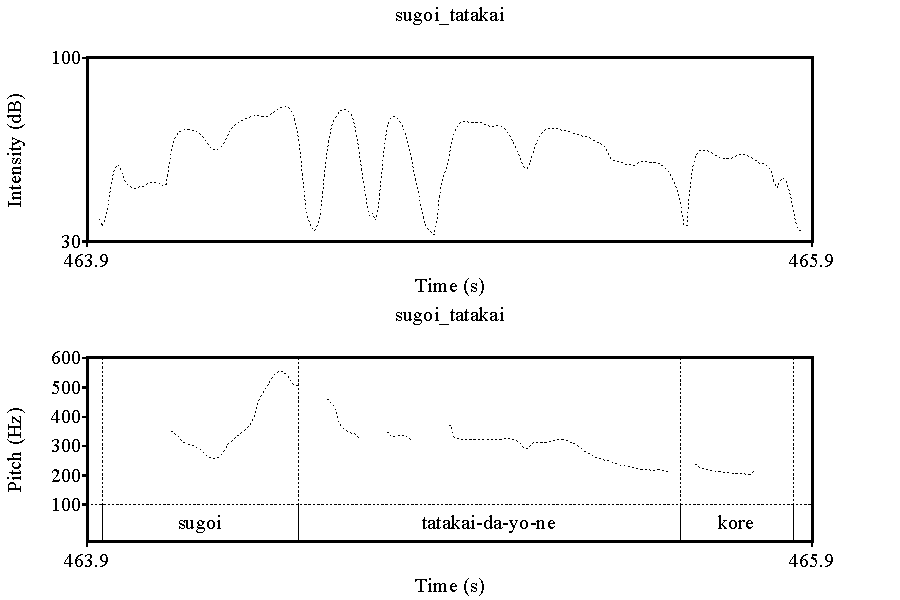
\includegraphics[width=0.6\textwidth]{sounds/D02F0025_sugoi_tatakai.pdf}
	\caption{Intensity and F$_{0}$ of single-contour type \ref{D02F0025_sugoi_tatakai}}
	\label{D02F0025_sugoi_tatakaiF}
	\end{center}
%\end{minipage}
\end{figure}
\begin{figure}
%\begin{minipage}{0.5\textwidth}
	\begin{center}
	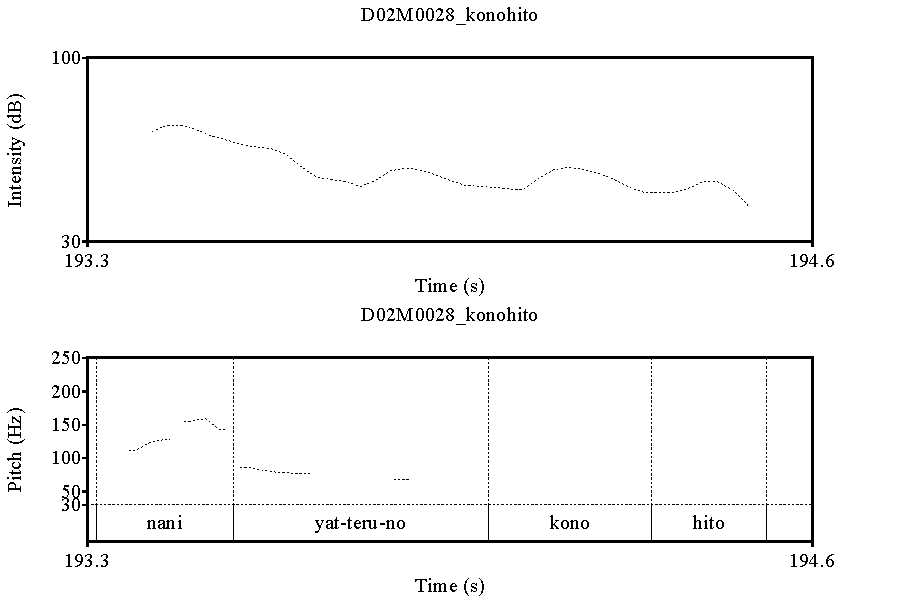
\includegraphics[width=0.6\textwidth]{sounds/D02M0028_konohito.pdf}
	\caption{Intensity and F$_{0}$ of single-contour type \ref{D02M0028_konohito}}
	\label{D02M0028_konohitoF}
	\end{center}
%\end{minipage}
\end{figure}
\begin{figure}
%\begin{minipage}{0.5\textwidth}
	\begin{center}
	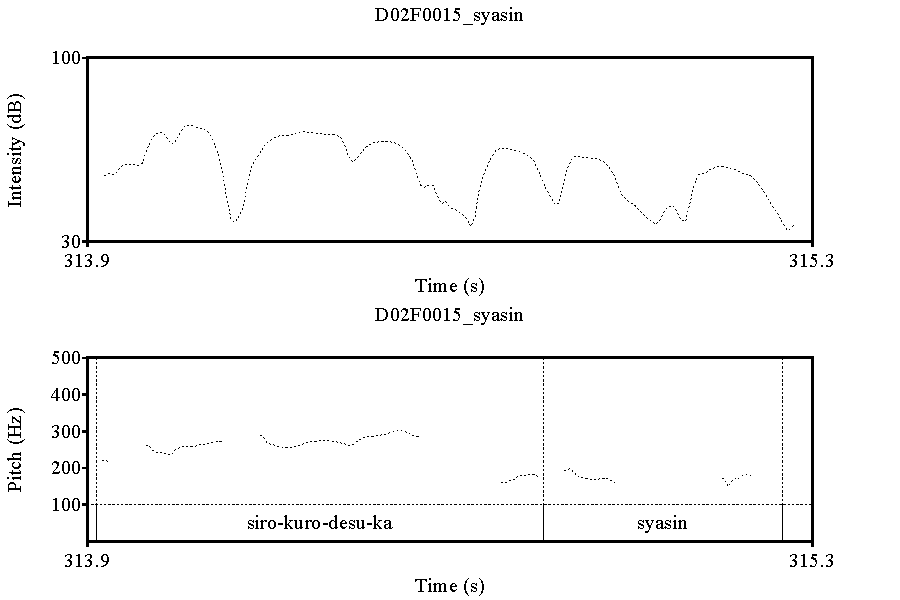
\includegraphics[width=0.6\textwidth]{sounds/D02F0015_syasin.pdf}
	\caption{Intensity and F$_{0}$ of single-contour type \ref{D02F0015_syasin}}
	\label{D02F0015_syasinF}
	\end{center}
%\end{minipage}
\end{figure}


On the other hand,
postposed elements of the double-contour type have not been evoked enough or they are contrastive at the time of \isi{utterance}.
In \Next, where again the participants are involved in the task of ranking famous people based on their income,
\ci{kotti-wa} `on my side' is uttered in a separate contour from the \isi{main clause} and there is a pause between the \isi{main clause} and the \isi{postposed element}, as shown in Figure \ref{D02F0015_kottiwaF}.
`On my side' is necessary information in the sense that
the other participant L was talking about how many people were listed on her own side.
Therefore, the participant R might have thought that `there are ten people' is not enough and added `on my side' later.
The F$_{0}$ peak of the postposed \ci{kotti-wa} `on my side' is still lower than \ci{zyuu} `ten' in the \isi{main clause},
and the intensity is also lower.
This is because the \isi{postposed element} is not the focus as \citeA{takami95a,takami95b} has pointed out.
Foci are typically new in the given-new taxonomy and need both F$_{0}$ peak and intensity in order for the \isi{hearer} to understand clearly what is said.
%
\ex.\label{D02F0015_kottiwa}
 \a.[L:] There are eleven people (listed on my side).
 \bg.[R:] zyuu-nin-desu \EM{kotti-wa} \\
 		ten-people-\ab{cop}.\ab{plt} this.side-\ci{wa} \\
		`There are ten people on my side.'
	\src{D02F0015: 3.27-9.03}

%Similarly in \Next,
%where the participants are involved in the same task,
%the participants were talking about how the compensation system works in the show business and .
%%
%\ex.\label{D02F0015_geenookai}
% \ag.[L:] kore-wa dan-zyo-no sa-wa nai-n-desu-ka-ne geenookai-tte \\
% 		this-\ci{wa} male-female-\ab{gen} difference-\ci{wa} not.exist-\ab{nmlz}-\ab{cop}.\ab{plt}-\ab{q}-\ab{fp} show.business-\ab{top} \\
%		`Isn't there difference between men and women (income), the show business?'
%	\src{D02F0015: 890.51-893.82}

In \Next,
L is interviewing R about her study on the difference among Japanese dialects.
R utters `western area' in a separate contour from the predicate
because R compares different dialects and, only in the eastern area, did she find no differences among smaller areas (prefectures).
Therefore `the eastern area' is contrasted with other areas.
In this case, the F$_{0}$ peak and the intensity of the \isi{postposed element} are as high as those of the \isi{main clause},
as shown in Figure \ref{D04F0050_kantooF}.
%
\ex.\label{D04F0050_kantoo}
 \ag.[R:] kooiu sa-ga aru-ne-tte iu-koto-wa ie-nai zyootai-desi-ta-ne \EM{kantoo-no} \EM{hoo-wa} \\
 	such.and.such difference-\ci{ga} exist-\ab{fp}-\ab{q} say-thing-\ci{wa} say-\ab{neg} situation-\ab{cop}.\ab{plt}-\ab{past}-\ab{fp} east-\ab{gen} direction-\ci{wa} \\
	`One cannot say that there is such and such difference, eastern area.'
	\src{D04F0050: 338.54-349.27}

\begin{figure}
%\begin{minipage}{0.5\textwidth}
	\begin{center}
	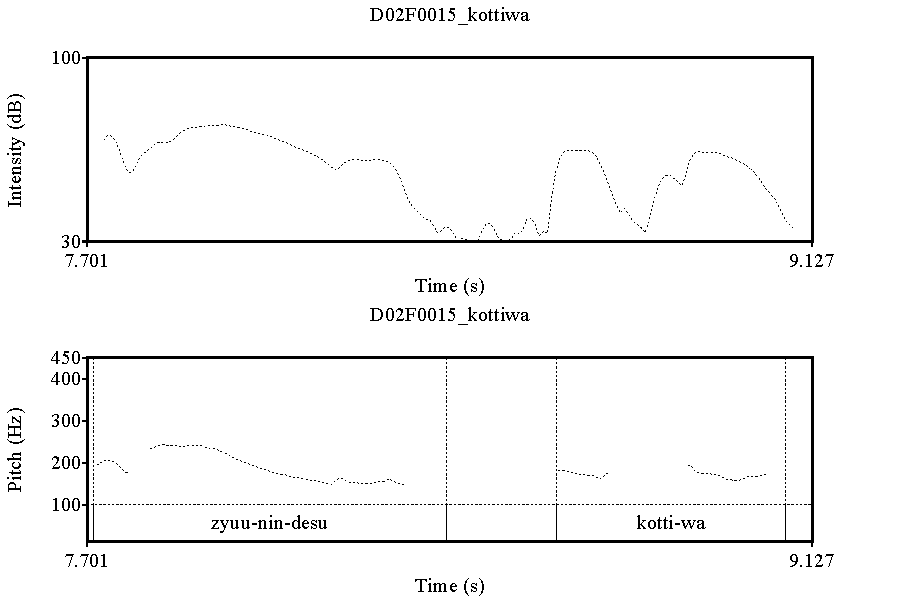
\includegraphics[width=0.6\textwidth]{sounds/D02F0015_kottiwa.pdf}
	\caption{Intensity and F$_{0}$ of double-contour type \ref{D02F0015_kottiwa}}
	\label{D02F0015_kottiwaF}
	\end{center}
%\end{minipage}
\end{figure}
\begin{figure}
%\begin{minipage}{0.5\textwidth}
	\begin{center}
	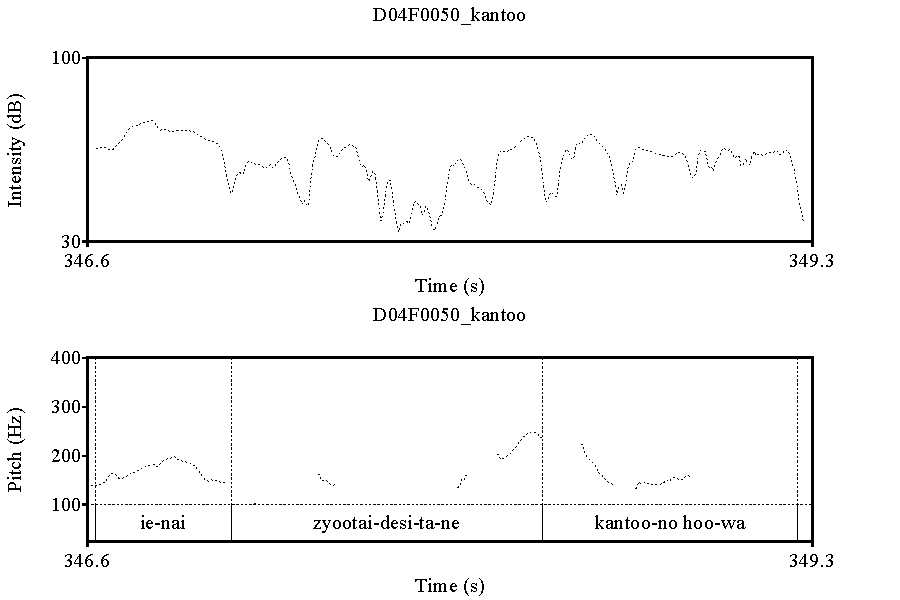
\includegraphics[width=0.6\textwidth]{sounds/D04F0050_kantoo.pdf}
	\caption{Intensity and F$_{0}$ of double-contour type \ref{D04F0050_kantoo}}
	\label{D04F0050_kantooF}
	\end{center}
%\end{minipage}
\end{figure}



%%----------------------------------------------------
\subsection{Motivations for topics to appear post-predicatively}\label{WO:PostP:Motivations}

It has been pointed out that
topics or given elements tend to appear clause initially \cite{mathesius28,firbas64,danes70}.
What are the motivations for them to appear post-predicatively?
In this section I mainly discuss the post-predicate elements of the single-contour type in comparison with the elements before the predicate.
Those of the double-contour type are heterogeneous as discussed above and this needs further investigation.


%%----------------------------------------------------
\subsubsection{Low activation cost and general characteristics of intonation unit}\label{WO:PostP:Motivations:IU}

Before getting directly into the question of
why some topics appear post-pred\-i\-cat\-ively, %
%%%ISSUE "post-predicatively" does not allign properly.
let us begin with the question of why some topics do not appear clause-initially.
As discussed in \S \ref{GivenAppearClause-Initially} and this section,
the \isi{activation cost} of preposed topics is higher than
those of postposed topics and zero pronouns.
The \isi{low activation cost} of post-predicate elements suggests that
they are not anchors to the previous \isi{discourse};
since they are already evoked enough,
they do not have to relate to the previous contexts and the current \isi{utterance}.
Therefore, they have the motivations for not appearing clause-initially.
Why do they appear post-predicatively?

I argue that the element whose \isi{activation cost} is low tends to appear post-predicatively
because, in Japanese and many other languages,
an \isi{intonation unit} starts from high F$_{0}$ and gradually declines toward the end 
\cite{libermanpierrehumbert84,cruttenden86,duboisetal93,chafe94,prieto96,truckenbrodt04,denetal10}.
Since the elements with \isi{low activation cost} do not require high F$_{0}$,
their preferred position is toward the last position in an \isi{intonation unit}.
This kind of phenomenon has already been reported in \ili{Siouan}, Caddoan, and \ili{Iroquoian} languages of North America \cite{mithun95}.
In these languages,
this newsworthy-first (i.e., given-last) \isi{word order} is fully grammaticalized, and Mithun proposes a hypothesis that the given-last \isi{word order} comes from right-detachment constructions, namely, the postposed constructions discussed in this section.
She argues that this \isi{word order} is motivated by the general tendency that intonation units start from high F$_{0}$, which gradually declines.
This tendency of intonation units is physiologically motivated,
as \citeA{cruttenden86} discusses:
%
\begin{quote}
The explanation for declination has often been related to the decline in transglottal pressure as the speaker uses up the breath in his lungs.
A more recent explanation suggests that an upward change of \isi{pitch} involves a physical adjustment which is more difficult than a downward change of \isi{pitch},
the evidence being that a rise takes longer to achieve than a fall of a similar interval in fundamental frequency.
\cite[][168]{cruttenden86}
\end{quote}
%

Moreover, \citeA[][89]{comrie89} argues that unstressed constituents such as \isi{clitic} pronouns are cross-linguistically ``subject to special positioning rules only loosely, if at all, relating to their \isi{grammatical relation}'';
therefore, he argues that ``sentences with pronouns can be discounted in favour of those with full noun phrases''.
%I believe that this tendency is also the case not only with pronouns but also given full NPs in Japanese
%because, in Japanese, pronouns are not very frequent and full NPs are frequently used to refer to activated referent and they are frequently unstressed \cite[\S 6.3]{venditti00}.
Arguing against the hypothesis \cite{givon79}
that one can reconstruct ancient \isi{word order} of a language based on \isi{pronominal} affixes and clitics,
Comrie suggests that the order of \isi{pronominal} affixes and clitics in a clause is more likely to be influenced by stress rhythm properties \cite[][218]{comrie89}.

I argue that the order of Japanese unstressed pronouns and NPs is also affected by phonetic constraints as Comrie suggests.
As will be discussed in Chapter \ref{Intonation},
some unstressed pronouns and NPs referring to highly evoked entities
lose \isi{pitch} peaks and are produced only in \isi{low pitch}.
However, an accent rule in Japanese does not allow lexical items to start with two \isi{low pitch} morae in a row.
Therefore, the best position for unstressed items is the sentence-final or \isi{post-predicate position},
which allows unstressed items to appear.
For phonetic analysis of unstressed items,
see Chapter \ref{Intonation}.


%%----------------------------------------------------
\subsubsection{Why the post-predicate construction mainly appears in dialogue and what the source of ``emotive'' usage is}

The declination of F$_{0}$ does not fully explain post-predicate constructions in Japanese.%
%%%ISSUE "Japanese" out of alignment.
The discussion above does not explain why the Japanese \isi{post-predicate construction} mainly appears in dialogues, but not in monologues.
Moreover, Japanese post-predicate constructions are reported to have ``\isi{emotive}'' characteristics \cite{ono07}.
As examples for \isi{emotive} characteristics of post-predicate constructions, consider the following constructed example.
Let us assume that a boy gave a present to his girlfriend.
The girl happily received the gift and opened it.
After seeing the gift, say a banana case,%
	\footnote{
	Bananas of all sizes can fit into this banana case.
	}
she uttered \Next or \NNext.
Since the most frequent \isi{word order} in Japanese is predicate-final,
the canonical order is \Next and
\NNext can be regarded as a \isi{post-predicate construction}.
%
\exg.\label{korenani}kore nani \\
	this what \\
	`What's this?'
	\hfill{(Canonical \isi{word order})}

\exg.\label{nanikore}nani kore \\
	what this \\
	`What's this (weird thing)?'
	\hfill{(Post-predicate construction)}

These two utterances consist of the same constituents \ci{kore} `this' and \ci{nani} `what'.
As was pointed out in \citeA{onosuzuki92} and \citeA{ono07},
however, the implicatures of these two are different.
In \LLast,
she simply does not know what she received,
probably because she has never seen it before.
By contrast, in \Last,
she knows what she received (it's a banana case) but she did not like it, as we expected.
\chd{In other contexts, \Last can be used to express the speaker's surprise,
excitement, etc.
However, \Last can never be a neutral question.}
Where does this \isi{implicature} come from?

Since these two utterances consist of exactly the same elements,
it is obvious that the \isi{implicature} in \Last cannot be derived from the meaning of each constituent.
In this study, I propose two factors involved in the questions of why post-predicate constructions mainly appear in dialogues and of what the source of this ``\isi{emotive}'' usage is:
\isi{word order} and intonation.

Firstly, I discuss why the \isi{post-predicate construction} appears mainly in dialogues.
My point is that,
since the intonation-unit-final position is a position for expressions with \isi{interactional} functions,
the \isi{post-predicate element} (of the single-contour type) plays some \isi{interactional} role.
As has traditionally been argued \cite[e.g.,][]{watanabe71},
the \isi{post-predicate position} is for interaction in Japanese.
\citeA{iwasaki93} extended this argument and claimed that
in fact the intonation-unit-final position is the position for interaction;
the \isi{post-predicate position} is only one example of this intonation-unit-final position.
Consider the following example.
Each line corresponds to a single \isi{intonation unit}.
The lines a, b, and c end with \isi{interactional} markers \ci{ne} and \ci{sa},
which is indicated by \EM{IT}.
As examples \Next show,
these \isi{interactional} markers appear IU-finally.%
	\footnote{
	IT stands for ``\isi{interactional} component'',
	one of four types of components in an \isi{intonation unit}.
	Other types are:
	LD (lead component (e.g., fillers)),
	ID (ideational component), and
%	SU (subjective component), and
	CO (cohesive component).
	The order of an \isi{intonation unit} is proposed to be
	LD ID CO IT in Japanese \cite[][44]{iwasaki93}.
	}
%
\ex.
 \a.
 \glll sooiu sito-ga siki si-te-\EM{ne} \\
 	such person-\ci{ga} lead do-and-\ab{fp} \\
	ID ID ID ID-CO-\EM{IT}	 \\
	\glt `Such people led, and'
 \b.
 \glll sinin-o asoko-e minna-\EM{ne} \\
 		corpses-\ci{o} there-\ab{dir} all-\ab{fp} \\
		ID ID ID-\EM{IT} \\
%	\glt `'
 \b.
 \glll ano dote-no ue-e-\EM{sa} \\
 		that bank-\ab{gen} top-\ab{dir}-\ab{fp} \\
		ID ID ID-ID-\EM{IT} \\
%	 \glt `'
 \glll atsume-te \\
 		gather-and \\
		ID-CO \\
	\glt `gathered dead bodies on top of that bank...'
	\hfill{\cite[][47, gloss and transcription modified by the current author]{iwasaki93}}

As \citeA{morita05} suggests,
a general function of \isi{interactional} particles such as \ci{ne} and \ci{sa} is ``to foreground a certain stretch of talk as an `interactionally relevant unit' to be operated on
-- whether that unit is itself a whole \isi{utterance} or merely one particular component of that \isi{utterance}'' (p.~92).
Since the post-predicate elements follows these \isi{interactional} particles within the same \isi{intonation unit} as in \ref{D02F0015_TerryIto} and \ref{D02F0025_sugoi_tatakai},
where the post-predicate elements follow \ci{ne},
they are also expected to have some \isi{interactional} functions.
\citeA{kakuden12} report that
77.6\% of the post-predicate constructions have \isi{interactional} particles of this kind after the predicate,
whereas only 47.0 \% of the non-post-predicate constructions have \isi{interactional} particles.
This also suggests that post-predicate constructions are related to
some \isi{interactional} characteristics.
Further investigation is necessary for the question of what kind of \isi{interactional} functions they have,
possibly employing conversational analysis.

Secondly,
I argue that 
the source of ``\isi{emotive}'' \isi{implicature} of \ref{nanikore} in contrast with \ref{korenani} comes from the intonational constraint of the \isi{post-predicate element}.
In Japanese, \ci{wh}-questions can be optionally uttered with \isi{rising intonation}.
%%% 要文献
However, the \isi{post-predicate element} is always falling and the \isi{rising intonation} is not natural.
Figure \ref{nanikoreF} shows the \isi{pitch contour} of the \isi{utterance} \ci{nani kore} `what's this (weird thing)?' \ref{nanikore},
while Figure \ref{korenaniF} shows the \isi{pitch contour} of neutral order \ci{kore nani} `what's this?' \ref{korenani}.
As indicated in the figures, the neutral \isi{word order} \ref{korenani} in Figure \ref{korenaniF} is uttered with \isi{rising intonation},
and I believe that this is the most frequent intonation,
whereas the \isi{post-predicate construction} \ref{nanikore} in Figure \ref{nanikoreF} is \isi{falling intonation},
in which case it is impossible to utter \ci{kore} with \isi{rising intonation}.
%Questions with \isi{falling intonation} convey negative emotion of the speaker.
It is this constraint on the intonation of post-predicate elements that yields the \isi{emotive} \isi{implicature} of the \isi{utterance} \ref{nanikore}.
In fact, the neutral \isi{word order} \ci{kore nani} can be uttered in \isi{falling intonation}, as shown in Figure \ref{korenani_fallF}.
In this case, as predicted from the discussion, the \isi{falling intonation} conveys emotion of the speaker.
It is possible for \ci{nani} `what' in \ref{nanikore} to be uttered with \isi{rising intonation} as indicated in Figure \ref{nanikore_riseF},
in which case the \isi{emotive} nuance of \ref{nanikore} disappears.


\begin{figure}
%\begin{minipage}{0.5\textwidth}
	\begin{center}
	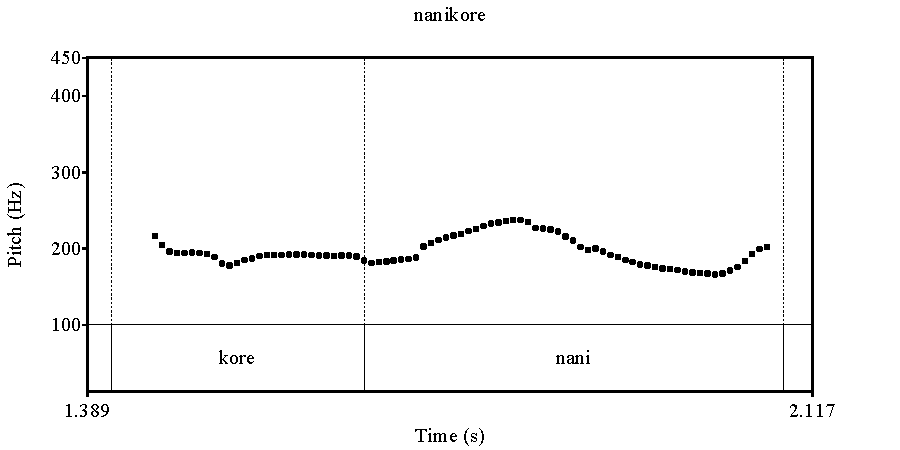
\includegraphics[width=0.6\textwidth]{sounds/korenani.pdf}
	\caption{Pitch contour of \ci{kore nani} \ref{korenani} with rising intonation}
	\label{korenaniF}
	\end{center}
%\end{minipage}
\end{figure}
\begin{figure}
%\begin{minipage}{0.5\textwidth}
	\begin{center}
	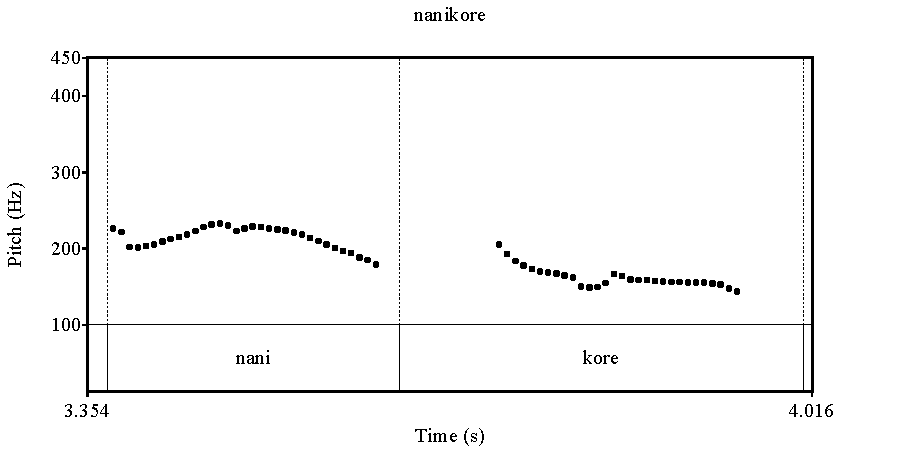
\includegraphics[width=0.6\textwidth]{sounds/nanikore.pdf}
	\caption{Pitch contour of \ci{nani kore} \ref{nanikore}}
	\label{nanikoreF}
	\end{center}
%\end{minipage}
\end{figure}
\begin{figure}
%\begin{minipage}{0.5\textwidth}
	\begin{center}
	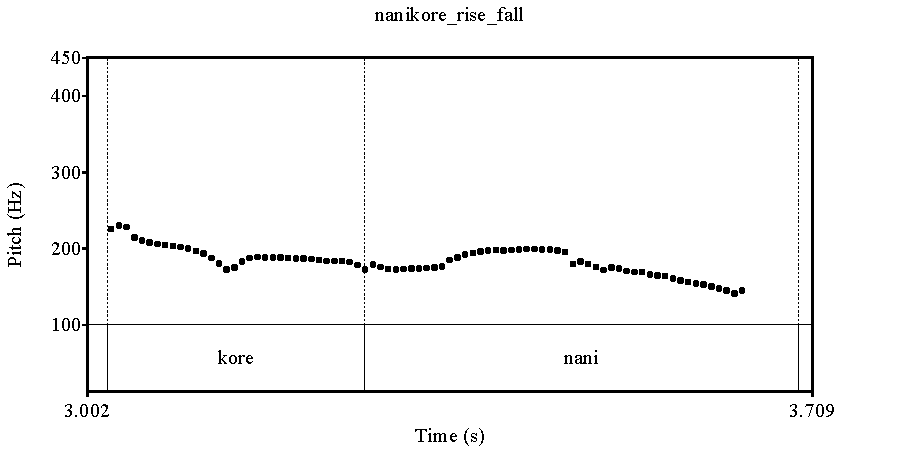
\includegraphics[width=0.6\textwidth]{sounds/korenani_fall.pdf}
	\caption{Pitch contour of \ci{kore nani} \ref{korenani} with falling intonation}
	\label{korenani_fallF}
	\end{center}
%\end{minipage}
\end{figure}
\begin{figure}
%\begin{minipage}{0.5\textwidth}
	\begin{center}
	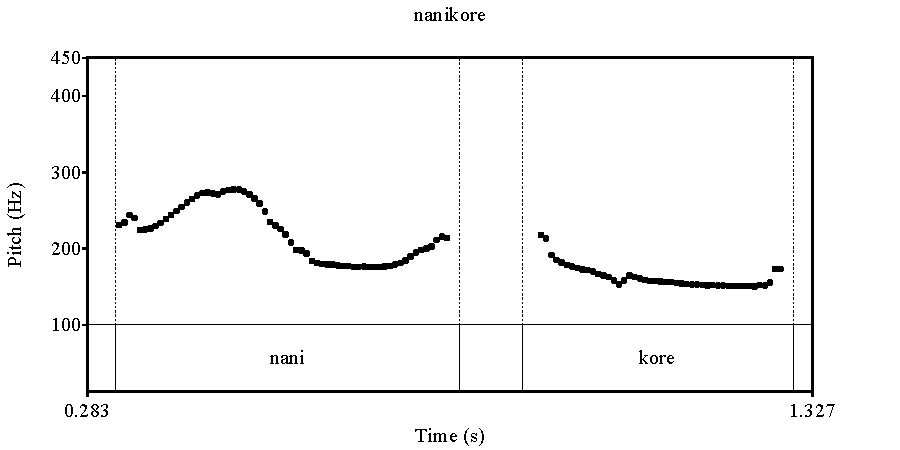
\includegraphics[width=0.6\textwidth]{sounds/nanikore_rise.pdf}
	\caption{Pitch contour of \ci{nani kore} \ref{nanikore} with rising intonation of \ci{nani}}
	\label{nanikore_riseF}
	\end{center}
%\end{minipage}
\end{figure}

%%----------------------------------------------------
\subsubsection{Post-predicate elements with double-contour type}\label{WO:PostP:Motiv:Double}

Finally, in this section,
I briefly mention intriguing studies on post-predicate constructions,
which I assume belong to the double-contour type.
The first study is \citeA{kakuden12}.
They investigated whether the \isi{hearer} responds (including back-channel responses) to the speaker near and after the predicate and showed that
the speaker adds post-predicate elements
when the \isi{hearer} does not respond to the predicate.
Their further analysis suggests that the speaker produces post-predicate elements to acquire the \isi{hearer}'s response and to achieve mutual belief.
Let us see example \Next,
which comes from the dialogue part of CSJ they employed.
The duration of silence is shown in seconds inside parentheses
since it is important for the discussion.
In \Next[-L2], where the speaker postposes the element \ci{kono kenkyuu} `this study',
there are pauses between the \isi{verb} phrase and the postposed \isi{demonstrative} \ci{kono} `this' and between the \isi{demonstrative} and the postposed NP \ci{kenkyuu} `study',
which is enough time for L to realize that
R does not respond to L.
Note that R, the listener of the \isi{postposed construction},
does not respond until 604.33 seconds,
0.32 seconds after L finished the post-predicate part.
Also note that
these pauses differentiate post-predicate constructions of the double-contour type from those of the single-contour type.
%
\ex.
 \ag.[L1:] ima nan-nin-gurai-de (0.588) a (0.29) ohi \\
           now what-\ab{cl}.person-\ab{hdg}-with {} \ab{fl} {} \ab{frg} \\
           `Right now, how many people... oh,'
 \bg.[L2:] kihontekini-wa hitori-de (0.161) \EMi{yat}-te rassyaru-desu-mon-ne
           (0.12) \EM{kono} (0.585) \EM{kenkyuu} \\
           basically-\ci{wa} alone-with {} do-and \ab{prog}.\ab{hon}-\ab{cop}-\ab{nmlz}-\ab{fp} {} this {} study \\
           `basically, (you) do (it) by yourself, this study?'
 \b.[] \src{D04M0010: 597.20-604.01}
 \bg.[R3:] ettoo (0.434) a (0.137) boku-no syozoku-si-teru kenkyuu-situ-de(0.44)-wa hanasi-kotoba-no ninsiki-o yat-teru-no-wa (0.143) m soo-desu-ne \\
           \ab{fl} {} \ab{fl} {} \ab{1}\ab{sg}-\ab{gen} belong-do-\ab{prog} study-room-\ab{loc}-\ci{wa} speech-language-\ab{gen} recognization-\ci{o} do-\ab{prog}-\ab{nmlz}-\ci{wa} {} \ab{frg} so-\ab{cop}.\ab{plt}-\ab{fp} \\
           `Lets see... in the lab I belong to the one who studies speech recognition is, yes...,'
 \bg.[R4:] boku hitori-desu-ne \\
      \ab{1}\ab{sg} alone-\ab{cop}.\ab{plt}-\ab{fp} \\
      `it's just me.'
           \src{D04M0010: 604.33-612.09}
  \b.[] \hfill{\cite[287]{kakuden12}}
%D04M0010|00597201L|597.201362|604.007857|L|今何人ぐらいで(0.588)(F あ)(0.29)(D おひ(? てぃ))基本的には一人で(0.161)やってらっしゃる(0.207)ですもんね(0.12)この(0.585)研究||倒置−つなぎ切り
%D04M0010|00604328R|604.327743|612.085642|R|(F えっとー)(0.434)(F あ)(D (? む))(0.137)僕の所属してる研究室で(0.44)は話し言葉の認識をやってるのは(0.143)(D む)そうですね僕一人ですね|[文末候補]|


\citeA{tanaka05} investigates postposed and preposed constructions
in terms of \isi{interactional} structures:
preferred vs.~dispreferred structures.
See the discussion in \S \ref{Back:CharJ:WO:PostP} for detail.
%Preferred structures include assessment followed by agreement and request followed by acceptance,
%while dispreferred structures include assessment followed by disagreement and request followed by refusal.
%According to \citeA[332ff.]{levinson83},
%preferred second parts including agreement with an assessment and acceptance of a request are typically produced in a 
%simple and direct form without delay;
%on the other hand,
%dispreferred second parts including disagreement with an assessment and
%refusal of a request are typically produced in a 
%complex and indirect form with delay.
%
%%
%\ex.
% \ag.[C:] ima-no katati-to mattaku onnazi.= \\
%          now-\ab{gen} shape-with exactly same \\
%          `(It's) exactly the same shape as the ones in vogue now.'
% \bg.[K:] =onnazi-yo$\downarrow$ =[\EM{eri-mo}. \\
%          same-\ab{fp} collar-also \\
%          `(It's) the same, the collar too.'
% \bg.[E:] {\hspace{2.45cm}} [a! honto::. \\
%          {} oh really \\
%          {\hspace{2.45cm}}`Oh re::ally.'
%          \hfill{\cite[406]{tanaka05}}
%
%\ex. (A response to an inquiry about an advertisement)
% \ag. ${\uparrow}$e:to{\textasciitilde}${\downarrow}$ g{\textasciitilde} (0.3) ano:: .hhhh \\
%      uh:m {} {} uh::m \\
%      `Uh:m- g- uh::m .hhhh'
% \bg. sono $<$\ul{nakami}$>$-made \\
%      its content-as.for \\
%      `when it comes down to its contents,'
% \bg. tyotto-ne \\
%      a.bit-\ab{fp} \\
%      `sort of'
% \bg. kookoku-no$\tilde{}$ gn $>$-ga-tte-no-wa \\
%      advert-\ab{gen} \ab{frg} -\ab{nom}-\ab{quot}-\ab{nmlz}-\ab{top} \\
%      `when it comes to the (gn) of the advert,'
% \bg. tyotto \\
%      a.bit \\
%      `sort.of'r
% \bg. kotira-de-wa \\
%      here-\ab{loc}-\ab{top} \\
%      `on our side,'
% \bg. wakara-nai-n-desu-keredomo$<$, .hhhh \\
%      know-\ab{neg}-\ab{nmlz}-\ab{cop}.\ab{plt}-though \\
%      `(we) have no knowledge of, .hhhh'
%       \hfill{\cite[412-413]{tanaka05}}

%%----------------------------------------------------
\subsection{Summary of post-predicate elements}

In this section
I investigated post-predicate elements.
It turned out that
the activation costs of postposed elements are much lower than
that of preposed elements,
which appear before the predicate.
This suggests that topics also appear post-predicatively.
I also discussed why
topics appear post-predicatively as well as clause-initially
in terms of the shape of intonation and its constraints on Japanese grammar.

The characteristic found in this study is one of many features of post-predicate elements.
In future research,
it is necessary to explore how these features are related to each other.


%%----------------------------------------------------
%%----------------------------------------------------
\section{Pre-predicate elements}\label{WOPrePredEles}

This section discusses pre-predicate elements,
which appear immediately before the predicate.
In \S \ref{WO:PreP:New},
I show results which indicate that
new, namely focus elements, elements tend to appear right before the predicate.
In \S \ref{WO:PreP:Motivation},
I discuss motivations for focus elements to appear near the predicate.

\begin{figure}
%\begin{minipage}{0.5\textwidth}
	\begin{center}
	\includegraphics[width=0.7\textwidth]{figure/DEPositionIS.pdf}
	\caption{Word order vs.\ information status}
	\label{DEPositionISF2}
	\end{center}
%\end{minipage}
\end{figure}
\begin{figure}
%\begin{minipage}{0.5\textwidth}
	\begin{center}
	\includegraphics[width=0.7\textwidth]{figure/DiffInfoStatus.pdf}
	\caption{Distance from predicate vs.\ InfoStatus}
	\label{DiffInfoStatusF2}
	\end{center}
%\end{minipage}
\end{figure}


%%----------------------------------------------------
\subsection{New elements appear right before predicate}\label{WO:PreP:New}

%\begin{figure}
%\begin{minipage}{0.5\textwidth}
%	\begin{center}
%	\includegraphics[width=0.95\textwidth]{figure/DiffCaseGiven.pdf}
%	\caption{}
%	\label{Diff1}
%	\end{center}
%\end{minipage}
%\begin{minipage}{0.5\textwidth}
%	\begin{center}
%	\includegraphics[width=0.95\textwidth]{figure/DiffCaseNew.pdf}
%	\caption{}
%	\label{Diff2}
%	\end{center}
%\end{minipage}
%\end{figure}
%
%\chd{
%According to the statistical analysis reported in \S \ref{WO:Intro},
%the effect of the distance between the element in question and the predicate to predict \isi{information status} is only marginally significant.
%}

As shown in Figure \ref{DEPositionISF} and \ref{DiffInfoStatusF},
which are repeated here for convenience as Figure \ref{DEPositionISF2} and \ref{DiffInfoStatusF2}, respectively,
new elements or focus elements tend to appear immediately before the predicate.
Figure \ref{DEPositionISF2} shows the element position based on their \isi{information status} including all expressions such as fillers, adjectives, and so on;
Figure \ref{DiffInfoStatusF2} shows the distance between the element and the predicate based on their \isi{information status}.
%Figure \ref{WOISGivenF2} and \ref{WOISNewF2} are histograms of position of arguments excluding other expressions and clauses with one argument.
%They also show the distribution of A, S, and P in each position.
As indicated in Figure \ref{DEPositionISF2},
the distribution of \isi{anaphoric} elements is skewed towards clause-initial position,
whereas that of non-\isi{anaphoric} elements is not.
Taking Figure \ref{DiffInfoStatusF2} into this account as well,
we can see that many of new elements appear immediately before the predicate.
%Considering clauses which contain equal to or more than two arguments,
%given elements appear at the initial position most frequently
%as shown in Figure \ref{WOISGivenF2},
%whereas new elements appear at the second position most frequently as shown \ref{WOISNewF2}.
%Especially given A elements are more frequent than new A elements in the initial position.
%This is compatible with the observation that A tend to be given in \ili{Sakapultec Maya} and many other languages \cite{dubois87,duboisetal03}.
%New S or P elements appear more frequently than given S or P elements in the second position.
\chd{As discussed in \ref{WO:Intro}, the mixed effects model of \isi{information status} (the distance between the predicate and the element in question) shows that
the contribution of the distance is only marginally significant.
However, a further analysis implies that the distance is also a significant factor for predicting \isi{information status}.
As is clear from Table \ref{ParInfoStatusCTT} and \ref{Par:InfoStatusPar:LSMEANST},
datives tend to code new elements (especially, as opposed to \ci{wa}).
Datives can appear anywhere, from pre-predicate to clause-initial positions,
which is shown in Figure \ref{WO:Prep:New:DiffASPF}.
%In fact, the model excluding datives indicates that
%both the distance and particles are significant factors to predict \isi{information status} (likelihood ratio test, $p<0.05$ without the distance, $p<0.001$ without particles).
Therefore, I tentatively conclude that the distance between the predicate and the element in question (excluding \ci{ni}-coded elements) is an important factor for \isi{information status} and
new elements appear before the predicate.
This supports a classic observation in other languages that focus appears closely with the predicate (\citeA{bresnan94,morimoto99} on Bantu languages, \citeA{jacennikdryer92} on \ili{Polish}, \citeA{erguvanli84} on \ili{Turkish}, see \citeA{morimoto00} for a summary of studies on both VO and OV languages).
Further studies are necessary to obtain conclusive evidence.}

\begin{figure}
	\begin{center}
	\includegraphics[width=0.8\textwidth]{figure/DiffASP.pdf}
	\caption{Distance from predicate vs.~grammatical functions}
	\label{WO:Prep:New:DiffASPF}
	\end{center}
\end{figure}


The following are example of non-\isi{anaphoric} elements appearing close to the predicate.
\Next and \NNext are examples of non-\isi{anaphoric} P occurring immediately before the predicate.
In \Next,
\ci{kyoomi} `interest' appear immediately before the predicate \ci{moti} `have',
and, in \NNext,
\ci{aidenthithii} `identity' in line a, \ci{inoti} `life' in line b, and \ci{ti} `blood' in line c appear right before the prediates \ci{kake} `risk' and \ci{nagasi} `bleed', respectively.
Non-\isi{anaphoric} Ps are typically abstract concepts like \ci{kyoomi} `interest' in \Next, \ci{aidenthithii} `identity' in \NNext[a], and \ci{inoti} `life' in \NNext[b], or
\isi{indefinite} like \ci{ti} `blood' in \NNext[c].
%
\exg. de ee sono ri-too-no hoo-ni sono \EM{kyoomi-o} \ul{moti} hazime-masi-te \\
		then \ab{fl} \ab{fl} remote-island-\ab{gen} direction-\ab{dat} \ab{fl} interest-\ci{o} have start-\ab{plt}-and \\
	`(We) are started to be interested in remote islands (in Hawaii).'
	\src{S00F0014: 149.92-153.33}
%S00F0014|00149920L|149.919959|153.334445|L|で(0.325)(F えー)(F その)離島の方に(F その)興味を持ち始めまして|/テ節/|

\ex.\label{S00M0199_inoti}
 \ag. tasuu-no serubia-zin-ga minzoku-no ee \EM{aidenthithii-o} \ul{kake}-te \\
 	many-\ab{gen} Serbia-people-\ci{ga} ethnic-\ab{gen} \ab{fl} identity-\ci{o} risk-and \\
	`Serbian people bet their identity, and'
 \bg. \EM{inoti-o} \ul{kake}-te \\
 		life-\ci{o} risk-and \\
		`risked their lives, and'
 \bg. \EM{ti-o} \ul{nagasi}-ta-to iu \\
 		blood-\ci{o} bleed-\ab{past}-\ab{q} say \\
		`bled (in battles),'
 \bg. rekisi-ga ee sono-go tenkai s-are-masu \\
 	history-\ci{ga} \ab{fl} that-later progress do-\ab{pass}-\ab{plt} \\
	`history went on this way.'
	\src{S00M0199: 343.53-351.77}
%S00M0199|00337016L|337.015835|351.772351|L|その時(0.488)(F えー)(F ま)その聖地(0.157)を(0.142)守るという意味で(F あのー)このコソボ平原において(0.422)(F えー)多数のセルビア人が民族の(0.204)(F えー)アイデンティティーを賭けて命を賭けて血を流したという(0.379)歴史が(0.17)(F えー)その後(0.167)展開されます|[文末]|

Non-\isi{anaphoric} S elements also appear immediately before the predicate.
They tend to be abstract or \isi{indefinite} like non-\isi{anaphoric} Ps.
In \Next,
\ci{kanzi} `impression' is the only argument of the predicate \ci{tigau} `differ' and hence is S,
which is an abstract concept.
This appears immediately before the predicate.
%
\ex.\label{S00F0014_kanzi}
 \ag. sono kontorasuto-toiuno-wa nanka totemo koo ekizotikku-to-iu-ka \\
 	that contrast-\ci{toiuno}-\ci{wa} somehow very such exotic-\ab{quot}-say-\ab{q} \\
	`The contrast (the color of black and blue) is very exotic, I would say,'
 \bg. husigina \EM{kanzi}-ga \ul{si}-masi-te \\
 		mysterious impression-\ci{ga} do-\ab{plt}-and \\
		`the impression was mysterious.'
		\src{S00F0014: 1042.88-1047.03}
%S00F0014|01042882L|1042.88247|1047.031717|L|そのコントラストというのは何かとてもこうエキゾチックと言うか不思議な感じがしまして|/テ節/|
%
%\ex.
% \ag. iya risu-nisite-wa tyotto sippo-no \EM{kanzi}-ga tigau-na-to \\
% 		no squirrel-for-\ci{wa} a.bit tail-\ab{gen} impression-\ab{nom} different-\ab{fp}-\ab{quot} \\
%		`No, the impression of (the animal's) tail is different from that of squirrels,'
% \bg. omot-te-ta-n-desu-ne \\
% 	think-\ab{prog}-\ab{nmlz}-\ab{cop}.\ab{plt}-\ab{fp} \\
%	`(I) was thinking like that.'
%	\src{S00F0014: 635.38-639.92}
%S00F0014|00635381L|635.381427|639.920666|L|いやリスにしてはちょっと尻尾の感じが違うなと(0.352)思ってたんですね|[文末]|

In \Next,
\ci{hito} `person' is \isi{indefinite} and appears before the predicate.
\exg. naka-ni-wa byooin-okuri-ni naru \EM{hito}-mo \ul{i}-masi-ta-kedomo \\
		inside-\ab{dat}-\ci{wa} hospital-send-to become person-also exist-\ab{plt}-\ab{past}-though \\
		`Some people were sent to the hospital (lit. People who were sent to the hospital also exist).'
		\src{S05M1236: 578.30-581.49}
%S05M1236|00578305L|578.304793|581.489255|L|中には病院送りになる(0.445)<笑>人もいましたけども|/並列節ケドモ/|


%%----------------------------------------------------
\subsection{Motivations for focus to appear close to predicate}\label{WO:PreP:Motivation}

%Why do non-\isi{anaphoric} elements most frequently appear close to the predicate?
I argue that the information-structure \isi{continuity principle} \ref{IScontinuityP} is also at work here, which is repeated below as \Next for the purpose of convenience.
%
\ex. \label{IScontinuityP2}\tl{Information-structure continuity principle}:
 A unit of \isi{information structure} is continuous in a clause;
 i.e., elements which belong to the same unit are adjacent with each other.

I assume that
most frequently the predicate is in the domain of focus \cite{lambrecht94},
optionally with one focus element.
Since the predicate and the new element are in the same domain of focus,
they appear together most frequently.

In fact, few studies pay attention to the \isi{information status} (and namely \isi{information structure}) of predicates.%
	\footnote{
	\citeA{hopperthompson80} is an important exception.
	}
Unfortunately this study is not an exception.
Typically definite markers such as \ci{the} in \ili{English} and \ci{der} in \ili{German} attach to nouns, not to verbs.
Also \isi{topic} markers such as \ci{wa} in Japanese typically attach to nouns.
Therefore, nouns have attracted more attention than verbs.
Typically verbs are followed by tense or aspect markers, subordinate-clause markers, realis vs.\ irrealis markers, and so on.
I believe that these verbal markers are also related to \isi{information structure},
but this is beyond the scope of this study.

However,
it is obvious that \isi{argument-focus structure},
where the predicate is not in the domain of focus,
is the least frequent type among all three types (predicate-focus, sentence-focus, and argument-focus structures).
Given that the corpus employed in this study consists of monologues, it is to be expected that there are even fewer examples of argument-focus structures because these structures typically appear as the answer to a who/what question, as shown in \Next where the capital letters indicate prominence.
%
\ex.
 \a.[Q:] Who went to school?
 \b.[A:] [The CHILDREN]$_{F}$ [went to school]$_{T}$.
 \hfill{\cite[][121]{lambrecht94}}

Since there are no (explicit) questions in monologues,
we find fewer argument-focus structures.

Another context in which sentences with \isi{argument-focus structure} appear is the ``A not B'' context.
In \isi{monologue}, ``A not B'' contexts typically appear in self-repair,
which is also rare in our relatively smooth monologues.
Therefore, it is not unreasonable to assume that the predicate is in the domain of focus most of the time,
and I argue that the information-structure \isi{continuity principle} \ref{IScontinuityP2} explains why new elements (i.e., focus elements) tend to appear immediately before the predicate.

One piece of evidence that supports the information-structure \isi{continuity principle} is the fact that
it is difficult for presupposed elements to appear immediately before the predicate,
interrupting the focus domain.
Compare \Next[A] and \Next[A$^{\prime}$],
which are assumed to be the answers to the question \Next[Q].%
	\footnote{
	Note that they are not a perfect minimal pair because of the \isi{accusative marker} of \ci{o}.
	The presence or absence of \ci{o} is determined by \isi{word order} and
	\isi{information structure} is a kind of side effect in this case.
	See the discussion in \S \ref{CasePar} for more detail.
	}
In \Next[A],
the presupposed elements \ci{taroo-ni} `to Taro' and \ci{hanako-ni} `to Hanako' are interrupting the domain of focus `gave a travel ticket' and `gave a cake'.
Therefore this sentence is not acceptable.
Conversely, in \Next[A$^{\prime}$],
the presupposed elements do not intervene the domain of focus and hence this is acceptable.
%
\ex.
 \a.[Q:] What did you do for Taro and Hanako for their birthdays?
 \bg.[A:] ?[ryokoo-ken-o]$_{F}$ [taroo-ni]$_{T}$ [age-te]$_{F}$ [keeki-o]$_{F}$ [hanako-ni]$_{T}$ [tukut-te age-ta]$_{F}$-yo \\
 			travel-ticket-\ci{o} Taro-\ab{dat} give-and cake-\ci{o} Hanako-\ab{dat} make-and give-\ab{past}-\ab{fp} \\
			`(I) gave travel tickets to Taro and gave cake to Hanako.'
 \bg.[A$^{\prime}$:] [taroo-ni]$_{T}$ [ryokoo-ken age-te]$_{F}$ [hanako-ni]$_{T}$ [keeki tukut-te age-ta]$_{F}$-yo \\
 			Taro-\ab{dat} travel-ticket give-and Hanako-\ab{dat} cake make-and give-\ab{past}-\ab{fp} \\
			`(I) gave travel Taro travel tickets and gave Hanako cake.'

A more natural context for \Last[A] is where Q asks
what A did for the travel ticket and the cake.
\citeA{kuno78} proposes that
the pre-predicate position is for new elements,
but he limits this principle to cases
where the predicate is given.
%
\ex.
 In cases where the predicate is given,
 the position immediately before the predicate is the position for new.
 \hfill{\cite[][60, translated by the current author]{kuno78}}

I argue that this observation also applies to cases where the predicate is new.

Moreover,
as will be discussed in Chapter \ref{Intonation},
the domain of focus is uttered in a single \isi{intonation unit},
whereas the \isi{topic} is uttered separately from the domain of focus.
Figure \ref{S00M0199_aidenthithiF} to \ref{S00F0014_kanziF} show
the \isi{pitch} contours of examples \ref{S00M0199_inoti} and \ref{S00F0014_kanzi} we discussed in the last section.
As we can see,
there is no pause between the predicate and the previous element and
the \isi{pitch range} is larger in the elements than in the predicates.
In Figure \ref{S00M0199_tiF},
it is difficult to see the \isi{pitch range} because \ci{ti} `blood' does not have accent nucleus.
From the first lowering of \ci{na} in \ci{nagasi-ta} `bled' being cancelled,%
	\footnote{
	The \isi{pitch accent} of \ci{nagasi-ta} is LHLL.
	}
one can see that
\ci{ti-o} `blood-\ci{o}' and \ci{nagasi-ta} `bleed' form a single \isi{intonation unit}.


\begin{figure}
%\begin{minipage}{0.5\textwidth}
	\begin{center}
	\includegraphics[width=0.6\textwidth]{sounds/S00M0199_aidenthithi.pdf}
	\caption{Pitch contour of a in \ref{S00M0199_inoti}}
	\label{S00M0199_aidenthithiF}
	\end{center}
%\end{minipage}
\end{figure}
\begin{figure}
%\begin{minipage}{0.5\textwidth}
	\begin{center}
	\includegraphics[width=0.6\textwidth]{sounds/S00M0199_inoti.pdf}
	\caption{Pitch contour of b in \ref{S00M0199_inoti}}
	\label{S00M0199_inotiF}
	\end{center}
%\end{minipage}
\end{figure}
\begin{figure}
%\begin{minipage}{0.5\textwidth}
	\begin{center}
	\includegraphics[width=0.6\textwidth]{sounds/S00M0199_ti.pdf}
	\caption{Pitch contour of c in \ref{S00M0199_inoti}}
	\label{S00M0199_tiF}
	\end{center}
%\end{minipage}
\end{figure}
\begin{figure}
%\begin{minipage}{0.5\textwidth}
	\begin{center}
	\includegraphics[width=0.6\textwidth]{sounds/S00F0014_kanzi.pdf}
	\caption{Pitch contour of b in \ref{S00F0014_kanzi}}
	\label{S00F0014_kanziF}
	\end{center}
%\end{minipage}
\end{figure}

%%----------------------------------------------------
\subsection{Summary of pre-predicate elements}

The results of this section showed that
new elements, namely focus elements, tend to appear right before the predicate.
A similar claim has been made by \citeA{kuno78} and \citeA{endo14}
through constructed examples.
This study supported their claim by examining naturally occurring utterances.
I also discussed motivations for the focus to appear right before the predicate.

%%----------------------------------------------------
%%----------------------------------------------------
\section{Discussion}\label{WODiscussion}

This section first discusses possible confounding effects on \isi{word order} in Japanese,
in particular in association with basic \isi{word order} (\S \ref{WO:Dis:Confounding}).
Second,
I discuss Giv{\'{o}}n's \isi{topicality} hierarchy (\S \ref{WO:Dis:Givon}).
I provide some counter-examples of this hierarchy and
propose to modify it.
Finally, 
I discuss the implications of this study's findings as regards \isi{word order} typology (\S \ref{WO:Dis:WOTypology}).



%%----------------------------------------------------
\subsection{Possible confounding effects}\label{WO:Dis:Confounding}

\begin{figure}
%\begin{minipage}{0.5\textwidth}
	\begin{center}
	\includegraphics[width=0.6\textwidth]{figure/DEPositionASPA.pdf}
	\caption{Word order of A}
	\label{DEPositionASPAF}
	\end{center}
%\end{minipage}
\end{figure}
\begin{figure}
%\begin{minipage}{0.5\textwidth}
	\begin{center}
	\includegraphics[width=0.6\textwidth]{figure/DEPositionASPS.pdf}
	\caption{Word order of S}
	\label{DEPositionASPSF}
	\end{center}
%\end{minipage}
\end{figure}
\begin{figure}
%\begin{minipage}{0.5\textwidth}
	\begin{center}
	\includegraphics[width=0.6\textwidth]{figure/DEPositionASPP.pdf}
	\caption{Word order of P}
	\label{DEPositionASPPF}
	\end{center}
%\end{minipage}
\end{figure}
\begin{figure}
%\begin{minipage}{0.5\textwidth}
	\begin{center}
	\includegraphics[width=0.6\textwidth]{figure/DEPositionASPDAT.pdf}
	\caption{Word order of dative}
	\label{DEPositionASPDATF}
	\end{center}
%\end{minipage}
\end{figure}


It is necessary to take other features into account
to see the exact effect of topichood and focushood on \isi{word order}.%
%%%ISSUE odd word break in "topichood".
Especially, the effect of ``basic \isi{word order}'' should not be ignored.
%I did not employ any statistical analysis because
%there are still not enough data in my corpus.
Here I provide some evidence to support my argument that
\isi{information structure} contributes to \isi{word order} in spoken Japanese.
Figure \ref{DEPositionASPAF} to \ref{DEPositionASPDATF} show
\isi{word order} and \isi{information status} of each type of grammatical function (A, S, P, and dative).
These figures indicate that
\isi{anaphoric} elements of all grammatical function types are still more likely to appear earlier in a clause than new elements.
A and S are more likely to appear earlier in a clause than P because of the basic \isi{word order}.
However, my argument still holds for the same grammatical function types.
In cases with new elements,
one can see the effect of basic \isi{word order};
the peak of S is 4,
which means the 4th position is the most popular for new S (Figure \ref{DEPositionASPSF}),
whereas the peak of P is 6, which means the 6th position is the most popular for new P (Figure \ref{DEPositionASPPF}).
The distribution of A is not clear because there are few examples.
But the trend still seems to hold for A.

%%----------------------------------------------------
\subsection{Giv\'on's topicality hierarchy and word order}\label{WO:Dis:Givon}

\citeA{givon83} proposes a hierarchy of \isi{topicality} \Next (terminology modified by the author).
``RD'' refers to referential distance,
which is one of the approximations to measure \isi{topicality}.
Low RD means high \isi{topicality},
while high RD means low \isi{topicality}.
%
\ex.\label{TopicHierarchy}
 \a.[$\uparrow$] High RD
 \b. Referential \isi{indefinite} NPs
 \b. Cleft/focus constructions
 \b. Y-moved NPs (`contrastive topicalization')
 \b. Preposed definite NPs
 \b. Neutral-ordered definite NPs
 \b. Postposed definite NPs
 \b. Stressed/independent pronouns
 \b. Unstressed/bound pronouns or grammatical agreement
 \b. Zero anaphora
 \b.[$\downarrow$] Low RD
 \hfill{\cite[][7]{givon83}}

Here I point out two counter-examples against this hierarchy.
First,
as has already been shown in Table \ref{RDPostT} and \ref{RDPreT},
which are repeated as Table \ref{RDPostT2} and \ref{RDPreT2} for convenience,
the average RD of elements in the clause-initial position (20.9) is lower than that in the second (23.0) or third positions (41.1).
To see this more in detail,
I divided the result of Table \ref{RDPreT2} based on grammatical function.
This is shown in Table \ref{RDASP}.
Regardless of whether the element is A, S, or P,
the overall tendency is that
the elements closer to the predicate have higher average RD.%
 \footnote{
 For now I do not have an explanation for S in the second position.
 It is necessary to test whether the difference between Ss in the first and the second positions is statistically significant or not.
 }
%%% 2Sに関しては説明が必要
The \isi{topicality} hierarchy \ref{TopicHierarchy} predicts that
clause-initial elements (d in \ref{TopicHierarchy}) is lower RD than that of elements in the neutral-ordered position (e in \ref{TopicHierarchy}).%
	\footnote{
	I assume that all elements that have antecedents (and namely RDs) are definite.
	}
Especially P is against the \isi{topicality} hierarchy \ref{TopicHierarchy},
according to which P in the second or third positions should have lower RD than P in the first position because the neutral position of P is the second or third positions in Japanese.
But this is not the case.
At least in Japanese,
the data show that
elements closer to the predicate have higher RDs
because the pre-predicate position is for focus and hence new elements.

\begin{table}[bht]
%\begin{minipage}{0.5\textwidth}
\centering
\caption{RD of post-predicate elements}
\begin{tabular}{lrr}
\toprule
  & Single-contour & Double-contour \\
\midrule
RD & 6.9 & 39.7 \\
\bottomrule
\end{tabular}
\label{RDPostT2}
%\end{minipage}
\end{table}
\begin{table}
%\begin{minipage}{0.5\textwidth}
\centering
\caption{RD of pre-predicate elements (based on argument order)}
\begin{tabular}{lrrrr}
\toprule
  &  1  & 2 & 3 \\
\midrule
RD & 20.9 & 23.0 & 41.1 \\
\bottomrule
\end{tabular}
\label{RDPreT2}
%\end{minipage}
\end{table}

\begin{table}
%\begin{minipage}{0.5\textwidth}
\centering
\caption{RD of pre-predicate elements (based on grammatical function)}
\label{RDASP}
\begin{tabular}{lrrr}
\toprule
		& 1	& 2	& 3 \\
\midrule
%	Ex	& 15.2	& 15.0 & --	\\
	A	& 10.3	& 47.3	& -- \\
	S	& 22.5	& 21.7	& 73.5 \\
	P	& 22.4	& 36.6	& 49.1 \\
\bottomrule
\end{tabular}
%\end{minipage}
\end{table}

Second,
the average RD of zero pronouns is as high as that of postposed NPs
according to Table \ref{RDPostExpTypeT} and \ref{RDPreExpTypeT}.
This is against the \isi{topicality} hierarchy \ref{TopicHierarchy}
because it states that
preposed definite NPs (d in \ref{TopicHierarchy}) and neutral-ordered definite NPs (e in \ref{TopicHierarchy}) have
higher RDs than
postposed definite NPs.
As discussed above,
elements are postposed for \isi{interactional} purposes and/or intonational reason.


\begin{table}
%\begin{minipage}{0.5\textwidth}
\centering
\caption{RD of postposed elements of the single-contour type (based on expression type)}
\begin{tabular}{lrr}
\toprule
  & Pronoun & NP \\
\midrule
RD & 15.1 & 5.0 \\
\bottomrule
\end{tabular}
\label{RDPostExpTypeT}
%\end{minipage}
\end{table}
\begin{table}
%\begin{minipage}{0.5\textwidth}
\centering
\caption{RD of pre-predicate elements (based on expression type)}
\begin{tabular}{lrrr}
\toprule
     & Zero & Pronoun & NP \\
\midrule
 RD  & 5.0  & 5.8     & 27.8 \\
\bottomrule
\end{tabular}
\label{RDPreExpTypeT}
%\end{minipage}
\end{table}

The final point is an additional suggestion of \ref{TopicHierarchy} rather than a counter-example.
The RD of postposed elements of the double-contour type is much higher than Giv\'on predicts.
As will be argued in Chapter \ref{Intonation},
a unit of \isi{information structure} corresponds to a unit of intonation.
Since postposed elements of the single-contour type by definition belong to the same \isi{intonation unit} as the main predicate,
the predicate and the \isi{postposed element} form a single unit (construction) and postposed elements are relatively homogeneous and easy to characterize.
However,
postposed elements of the double-contour type are heterogeneous as discussed above and are difficult to characterize
because the element itself corresponds to a single unit.
The motivations for such elements to be uttered are heterogeneous.
The functions of such postposed elements are determined by the sequence of conversation.


%%----------------------------------------------------
\subsection{Information structure and word order typology}\label{WO:Dis:WOTypology}

Since most frequent focus elements are patients according to the correlating features \ref{ISFeatures},
which is repeated as \Next,
the information-structure \isi{continuity principle} \ref{IScontinuityP} predicts that cross-linguistically
P (the patient-like argument in a \isi{transitive clause}) and V (the predicate) tend to appear together most frequently and,
if the \isi{word order} is fixed in the language in question,
P and V tend to appear together.
%
\ex.
\begin{tabular}{lll}
	 & \isi{topic} & focus \\
	a. & presupposed & asserted \\
	b. & evoked & brand-new \\
	c. & definite & \isi{indefinite} \\
	d. & specific & non-specific \\
	e. & \isi{animate} & \isi{inanimate} \\
	f. & agent & patient \\
	g. & \isi{inferable} & non-\isi{inferable} \\
%	h. & entity & proposition \\
\end{tabular}
%

In fact this has already been claimed and tested in \citeA[Chapter 4]{tomlin86}.
Tomlin proposes this claim as Verb-Object Bonding.
%
\ex. \tl{Verb-Object Bonding (VOB):}
	the object of a \isi{transitive verb} is more tightly bounded to the \isi{verb}
	than is its subject.
	\hfill{\cite[][74]{tomlin86}}
%``[i]n general the object of a \isi{transitive clause} is syntactically and semantically more tightly `bound' to the \isi{verb} than is the subject of a \isi{transitive clause}'' (p.~73).

He also states that
``[e]xactly why there should be such a bond between a \isi{transitive verb} and its object is not entirely clear'' (ibid.).
I propose the information-structure \isi{continuity principle}
for the motivation of such bond.
He enumerates many cross-linguistic pieces of evidence that support VOB.
I introduce a few of them to keep the discussion simple.

First,
in many languages,
there exists some clause-level phonological behavior
(reductions or sandhis) which occur between object and \isi{verb},
but not between subject and \isi{verb} (op.~cit., p.~97).
In \ili{French}, for example,
liaison does not occur between the subject and the \isi{transitive verb},
but it does between the object and the \isi{verb} \cite[see also][]{selkirk72}.
There is no liaison between the subject \ci{les gens} and the \isi{verb} \ci{ach\`{e}tent} as in \Next,
whereas there can be liaison between the \isi{verb} \ci{donnerons} and the object \ci{une pomme} as in \NNext.%
%%%ISSUE IPA fonts (inside the command \tp{}) are not shown properly.
%
\ex.
 \a. \glll
	les gens ach\`{e}tent beaucoup de \c{c}a \\
	\tp{le} \tp{Z\~a} \tp{aSEt} \tp{boku} \tp{d@} \tp{sa} \\
	the people buy.\ab{3}\ab{pl} much of that \\
	`Those people buy a lot of that.' \hfill{(no liaison)}
 \b. *\tp{le} \tp{Z\~a} \tp{zaSEt} \tp{boku} \tp{d@} \tp{sa} 
 		 \hfill{(*liaison)}

\ex.
 \a. \glll
	nous donnerons une pomme \`a notre m\`ere \\
  	\tp{nu} \tp{dOn@r\~o} \tp{zyn} \tp{pOm} \tp{a} \tp{notr} \tp{mEr} \\
	we give.\ab{3}\ab{pl} a apple to our mother \\
	`We will give an apple to our mother.'
	\hfill{(liaison)}
\begin{flushright}
\cite[][pp.~98-99, transcription modified based on standard \ili{French}]{tomlin86}
\end{flushright}

Another case is \ili{Yoruba} (Niger-Congo) \isi{vowel} deletion \cite[from][]{bamgbose64}.
In verb-noun sequences of this language,
when the object begins with a \isi{vowel},
the last \isi{vowel} of the \isi{verb} is sometimes deleted.
This happens between \isi{verb} and object, but not between subject and \isi{verb}.
%
\ex.
 \ag. \tp{gb\'e} + \tp{od\'o} $\to$ \tp{gb'\'od\'o} \\
		brought + motor \\
 \bg. \tp{jE} \tp{iy\'On} $\to$ \tp{j'iy\'On} \\
 		eat pounded.yam \\
 \bg. \tp{Se} \tp{\`ow\`o} $\to$ \tp{S'\`ow\`o} \\
 		do trade \\
		\hfill{\cite[][pp.~29--30]{bamgbose64}}

These phonological phenomena in \ili{French} and \ili{Yoruba} suggest that
the object and predicate are bound more tightly than the subject and predicate.
In a similar manner,
in Japanese,
the focus element and the predicate form a single \isi{intonation unit},
but the \isi{topic} element and the predicate do not,
as we will see in Chapter \ref{Intonation}.

The second piece of evidence that supports VOB is \isi{noun incorporation}.
In \ili{Mokilese} (Oceanic), for example,
there is a set of verbs into which an \isi{indefinite} object may be incorporated \cite[from][]{harrison76}.
\Next[a] is a \isi{transitive clause} with definite object,
which is not incorporated into the \isi{verb},
whereas \Next[b] is a clause with \isi{indefinite} object,
which is incorporated into the \isi{verb}.
Note that the incorporate object \ci{rimeh} `bottle' in \Next[b] is between the \isi{verb} and the aspect suffix \ci{la}.
%
\ex.
 \ag. ngoah audoh-\EMi{la} \EM{rimeh}-i \\
		\ab{1}\ab{sg} fill-\ab{pfv} bottle-this \\
		`I filled this bottle.'
 \bg. ngoah audohd \EM{rimeh}-\EMi{la} \\
		\ab{1}\ab{sg} fill bottle-\ab{pfv} \\
		`I filled bottles.'
		\hfill{\cite[162]{harrison76}}

Similarly,
compare \Next[a] and \Next[b].
\Next[a] is a case where the object \ci{suhkoah} `tree' is definite and is not incorporated,
while \Next[b] is a case where the object is \isi{indefinite} and is incorporated into the \isi{verb}.
\ex.
 \ag. ngoah poadok-\EMi{di} \EM{suhkoah}-i \\
 	\ab{1}\ab{sg} plant-\ab{pfv} tree-this \\
	`I planted this tree'
 \bg. ngoah poad \EM{suhkoah}-\EMi{di} \\
 	\ab{1}\ab{sg} plant tree-\ab{pfv} \\
	`I planted trees.'
	\hfill{(ibid.)}

As \citeA{mithun84} observes,
in some languages patient S can also be incorporated into verbs
but languages allows patient S-incorporation also allows P-incorporation (See also \citeA{baker88}).%
%%%ISSUE "P-incorporation" does not align properly.
Namely, there is a universal hierarchy as in \Next.
The last two (agent S and A) are in brackets because
they are not attested.
%
\ex. \label{NIhierarchy}P $>$ patient S ($>$ agent S $>$ A)

In Southern Tiwa (Tanoan), for example,
the patient Ss `dipper' and `snow' are incorporated as in \Next,
while the agent Ss such as `dog' cannot be incorporated as in \NNext.
	\ex. \ag. \tp{l-\EM{k'uru}-k'euwe-m} \\
			{\sc B}-\EM{dipper}-old-\ab{pres} \\
			`The dipper is old.'
		\bg. \tp{we-\EM{fan}-lur-mi} \\
			{\sc C}.\ab{neg}-\EM{snow}-fall-\ab{pres}.\ab{neg} \\
			`Snow isn't falling. (It is not snowing.)'  \hfill{(patient S)}
		\b.[] \hfill{\cite{allenetal84,baker88}}
	
	\ex. \ag. \tp{\EM{khwien}-ide} \tp{{\O}-teurawe-we} \\
			\EM{dog}-{\sc suf} {\sc A}-run-\ab{pres} \\
			`The dog is running.'
		\bg. *\tp{{\O}-\EM{khwien}-teurawe-we} \\
			{\sc A}-\EM{dog}-run-\ab{pres} \\
			`The dog is running.'
			\hfill{(agent S)}
		\b.[] \hfill{\cite{allenetal84,baker88}}

In Japanese,
\citeA{kageyama93} reports that
patient S and P (in his terminology, internal arguments) are widely incorporated into verbs and form noun-\isi{verb} compounds.
He also reports the existence of agent S and A (external arguments) incorporated into verbs,
but claims that they are exceptional.
%%% 例を追加
The hierarchy of \isi{noun incorporation} \ref{NIhierarchy} is similar to the hierarchy of zero-marking in Japanese.
This is because
they are both hierarchy based on focus structure (see also \S \ref{Disc:HardConst}).

Finally, VOB and the information-structure \isi{continuity principle} with correlating features of \isi{information structure} \ref{ISFeatures} predict that
cross-linguistically,
P and V appear together most frequently.
Table \ref{wals-81} shows the order of subject (S in the table, A in our term), object (O in the table, P in our term), and \isi{verb} \cite{wals-81}.
``[O]ne order is considered dominant if text counts reveal it to be more than twice as common as the next most frequent order; if no order has this property, then the language is treated as lacking a dominant order for that set of elements '' \cite{wals-s6}.
The table shows that
SOV and SVO are the most popular dominant \isi{word order} among all other possibilities as predicted,
while the next popular order is VSO,
which is against our prediction.
However, note that in deciding which \isi{word order} is dominant in a language,
Dryer included only
``a \isi{transitive clause}, more specifically declarative clauses in which both the subject and object involve a noun (and not just a \isi{pronoun})'' \cite{wals-81}.
Therefore, this dominant \isi{word order} might not be of \isi{predicate-focus structure}.
Since both of the full noun phrases can be new,
the clause might be of sentence-focus structure.
\citeA{dryer97} (as well as \citeA{wals-81}) points out that
\isi{transitive} clauses with full lexical nouns do not occur frequently;
it is more common that
one of the two arguments is \isi{pronominal},
which is more likely to be of \isi{predicate-focus structure}.
For now,
cross-linguistic examination of word orders controlling \isi{information structure} is very difficult
and I leave this problem for future studies.

\begin{table}
%\begin{minipage}{0.5\textwidth}
\centering
\caption{Order of subject, object, and verb \cite{wals-81}}
\label{wals-81}
\begin{tabular}{lr}
	\toprule
	Word Order & \# of Lgs \\
	\midrule
	SOV &	565 \\
	SVO &	488 \\
	VSO &	95 \\
	VOS &	25 \\
	OVS &	11 \\
	OSV &	4 \\
	No dominant order &	189 \\
	\bottomrule
\end{tabular}
\end{table}



% 「太郎が本は読んでるよ」ContrastiveならOKの理由


%%%----------------------------------------------------
%\subsection{Kuno's information order theory}

%%% 「[太郎は]T [何回]F [ヨーロッパに行った]Tの?」




%%----------------------------------------------------
%%----------------------------------------------------
\section{Summary}

%%----------------------------------------------------
\subsection{Summary of this chapter}

This chapter analyzed associations between \isi{word order} and \isi{information structure} in spoken Japanese.
I made it clear that
shared topics appear clause-initially,
while strongly evoked topics appear post-predicatively.
Also, new, i.e., focus, elements appear immediately before the predicate.
Based on these findings,
I proposed the information-structure \isi{continuity principle},
in addition to from-old-to-new principle and persistent-element-first principle.


%%----------------------------------------------------
\subsection{Remaining issues}

As I briefly discussed in \S \ref{WO:Dis:Confounding},
\isi{information structure} is not the only feature contributing to \isi{word order} in spoken Japanese.
It is necessary to employ statistical analyses.












% !TEX root = ../main.tex
\chapter{Intonation}\label{Intonation}


%%% 「興味を持つ」(S00F0014)など「興味」が低くて「持つ」の方が高い場合にSUU boundaryが設けられているが、これを不要と提案する
%%% 挿入節、引用節が1つのIUで言われるのは、これが1つのunitであるということを示す必要があるという別の動機がある
%%% 1つのIUにどれだけの情報を詰め込めるか、One New Idea Hypothesisとの観点から
%%% IUには、activation costとフォーカスという2つの要因が働いている
%%% 「Xφ」でポーズを置いて発話すれば題目として理解しやすく、ポーズを置かなければ一体的に把握しやすい[が相対的な問題である] (丹羽, 2006: p.290)
%%% Venditti (2000) の結果に言及
%%% Matsumoto (2003: 81): ``what lead NPs indicate about discourse production in the form of IUs is that one of the IU production strategies Japanese speakers employ is to first utter an independent NP IU and then use that NP as a `stepping stone' to build a complete proposition by incorporating that same previously uttered NP or a slightly formally revised NP in the next clausal IU.''

%%----------------------------------------------------
%%----------------------------------------------------
\section{Introduction}\label{Int:PIUCIU}

This chapter investigates the relation between information structure and intonation units.
I propose that
an intonation unit corresponds to a chunk of information, which often corresponds to a unit of information structure.
I employ two methods;
one is a corpus study that I have employed in the previous chapters (\S \ref{Int:IUISUnitCorp}),
and the other is a production experiment, where I ask native speakers of Japanese to read aloud sentences and measure F$_{0}$ of their speech (\S \ref{Int:IUISUnitExp}).
From these findings and the results of the experimental study,
I propose principles governing intonation (\S \ref{Int:Disc}).


Before going into the analyses,
I discuss two types of intonation units (IUs) investigated in this study:
phrasal IU and clausal IU.
For the definition of intonation units,
see \S \ref{BackSubIntonation}.

%%%----------------------------------------------------
%\subsection{Phrasal vs.~clausal IU}

I assume that there are many factors to determine IUs
and it is impossible to investigate all of them.
To study information structure factors determining IUs,
I distinguish two types of intonation units:
phrasal IU and clausal IU.
A phrasal IU is an IU where an element (NP regardless of grammatical functions) is uttered in an IU separate from its predicate, whereas
a clausal IU is an IU where an element is uttered in the same IU as its predicate.
IUs where elements themselves are predicates are excluded from the analysis.
Phrasal and clausal IUs are schematized as in \Next,
where an IU corresponds to a box.
%
\ex.
 \a. Phrasal IU: \fbox{NP} \fbox{Predicate}
 \b. Clausal IU: \fbox{NP Predicate}

The motivations for this distinction come from the observation that IUs in Japanese are more frequently smaller units than a clause \cite{iwasaki93},
while IUs in English often correspond to a clause \cite{chafe94}.
This distinction is also employed in \citeA[Chapter 4]{matsumoto03},
who investigated intonation units in Japanese in terms of information flow.
\Next is an example of Japanese IU,
where a single line corresponds to a single IU.
%
\ex.
 \ag. atasi-wa-ne \\
 		\ab{1}\ab{sg}-\ci{wa}-\ab{fp} \\
 \bg. uti-de kii-ta-no-ne \\
 	home-\ab{loc} listen-\ab{past}-\ab{nmlz}-\ab{fp} \\
 \bg. sono are-wa-ne \\
 	\ab{fl} that-\ci{wa}-\ab{fp} \\
 \bg. hoosoo-wa-ne \\
 	broadcast-\ci{wa}-\ab{fp}\\
 \bg. kazoku-de \\
 	family-with \\
	`I listened to the broadcast at home with my family.'
	\hfill{\cite[][p.~40]{iwasaki93}}

Iwasaki states that IUs in \Last are typical examples in Japanese.
An IU corresponds to a phrase rather than a clause.
Note that the definitions of IU in \citeA{iwasaki93} and \citeA{matsumoto03} are different from those in \citeA{denetal10} and \citeA{denetal11} employed in this study,
while they share some similarities.
In this particular example \Last,
most IUs end with the discourse particle \ci{ne},
which often appears IU-finally also in the criteria of Den et al.

%As discussed in \citeA{matsumoto03} and as will be discussed below,
%clausal IUs are more frequent than phrasal IUs also in Japanese and
%they are considered to be default IUs.
%Therefore, in the following sections,
%the main question is what kind of factors affect the speaker to produce phrasal IUs.

%%----------------------------------------------------
%%----------------------------------------------------
\section[IU and IS unit: corpus study]{Intonation unit and unit of information structure: corpus study}\label{Int:IUISUnitCorp}

\begin{table}
%\begin{minipage}{0.5\textwidth}
\centering
 \tblcaption{IU vs.~information status}
 \label{IUInfoStatusT}
 \begin{tabular}{lrr}
 \toprule
             & Anaphoric & Non-anaphoric \\
 \midrule
  Phrasal IU & 501   & 571 \\
             & \rt{(65.2\%)} & \rt{(59.4\%)} \\
  Clausal IU & 267   & 391 \\
             & \rt{(34.8\%)} & \rt{(40.6\%)} \\
 \midrule
  Sum        & 768   & 962  \\
             & \rt{(100\%)} & \rt{(100\%)} \\
 \bottomrule
 \end{tabular}
%        Phrasal Clausal
%  Anaphoric     501     267
%  Non-anaphoric       571     391
%\end{minipage}
\end{table}

\begin{table}
%\begin{minipage}{0.5\textwidth}
\centering
 \tblcaption{IU vs.~Persistence}
 \label{IUPerT}
 \begin{tabular}{lrr}
 \toprule
             & Persistent & Non-Persistent \\
 \midrule
  Phrasal IU & 524        & 548 \\
             & \rt{(63.2\%)} & \rt{(60.8\%)} \\
  Clausal IU & 305        & 353 \\
             & \rt{(36.8\%)} & \rt{(39.2\%)} \\
 \midrule
  Sum        & 829        & 901  \\
             & \rt{(100\%)} & \rt{(100\%)} \\
 \bottomrule
 \end{tabular}
%                 Phrasal Clausal
%  Persistent         524     305
%  Non-Persistent     548     353
%\end{minipage}
\end{table}

\begin{figure}
%\begin{minipage}{0.5\textwidth}
	\begin{center}
	\includegraphics[width=.5\textwidth]{figure/IUInfoStatus.pdf}
	\caption{IU vs.~information status}
	\label{IUInfoStatusF}
	\end{center}
%\end{minipage}
\end{figure}
\begin{figure}
%\begin{minipage}{0.5\textwidth}
	\begin{center}
	\includegraphics[width=.5\textwidth]{figure/IUPer.pdf}
	\caption{IU vs.~persistence}
	\label{IUPerF}
	\end{center}
%\end{minipage}
\end{figure}


%Since there are expected to be many factors affecting the distinction between phrasal vs.\ clausal IU,
%I conducted logistic regression analysis using R.
%Table \ref{IntonationGlmT} shows the results of the analysis,
%where the dependent variable is the distinction between phrasal (\code{1}) vs.\ clausal (\code{0}) IUs, and
%the independent variables are the following.
%%
%%\ex.
%% \a. Information Status: anaphoric (\code{1}) and non-anaphoric (\code{0})
%% \b. Persistence: persistent (\code{1}) and non-persistent (\code{0})
%% \b. Topic markers: \code{toiuno-wa}, \code{wa}, and \code{mo}
%% \b. grammatical function: \code{A}, \code{S}, \code{P}, and \code{LOC}
%% \b. Word order: \code{1}, \code{2}, \code{3}, and \code{4}
%
%\code{A} in \Last[d] indicates the agent-like argument of a transitive clause,
%\code{S} indicates the only argument of an intransitive clause,
%\code{P} indicates the patient-like argument of a transitive clause, and
%\code{LOC} indicates locative, or elements potentially coded by \ci{ni}.%
%	\footnote{
%	As discussed earlier, both dative and locative are coded by the same form \ci{ni} in Japanese.
%	In this paper, I do not distinguish between dative and locative
%	and call them together locatives.
%	}
%The numbers in \Last[e] represent the order of arguments (A, S, P, and locatives).
%\code{1} indicates that the argument appears in the initial position,
%\code{2} indicates that it appears in the second position, and so on.
%Those variables whose p-values are more than $0.1$ are not shown in table \ref{IntonationGlmT}.
%
%I will discuss the relation between the dependent variable and each independent variable in the following sections.

This section explores the associations between IUs and information structure by investigating our corpus.
I will argue that, in general, topics tend to be uttered in phrasal IUs (\S \ref{Int:IUISUnitCorp:Topic}),
while foci tend to be produced in clausal IUs (\S \ref{Int:IUISUnitCorp:Focus}).
I also discuss exceptional cases for each tendency.

\chd{Table \ref{IUInfoStatusT} and Figure \ref{IUInfoStatusF} show the distribution of phrasal vs.~clausal IUs
in different information statuses (anaphoric vs.~non-anaphoric).
Anaphoric elements refer to those whose referents have been mentioned in the previous discourse,
whereas non-anaphoric elements refer to those whose referents have newly mentioned
(see \ref{FW:Cor:TopFoc} for the annotation procedure more in detail).
A linear mixed effects model was employed to predict information status, as we have seen in \S \ref{TopPar} and \S \ref{WO:Intro}.
Intonation (phrasal vs.~clausal IU), particles (\ci{toiuno-wa, wa, mo, ga, o, ni}), and word order (\code{nth} in CSJ, see \S \ref{WO:Intro} for the definition of this annotation) are included as fixed effects, and
the speaker (\code{TalkID} in the corpus) is included as a random effect.
The model with the effects of intonation, particles, and word order is significantly different from that without each of them (likelihood ratio test, $p<0.05$ without intonation, $p<0.001$ a model without particles, and $p<0.01$ that without word order).
}

\chd{
Table \ref{IUPerT} and Figure \ref{IUPerF} show the distribution of phrasal vs.~clausal IUs in terms of persistence
(persistent vs.~non-persistent).
Persistent elements are those whose referents are to be mentioned again in the following discourse,
whereas non-persistent elements are those whose referents are not to be mentioned.
Again a linear mixed effects model was applied to predict persistence, as discussed in \S \ref{TopPar} and \S \ref{WO:Intro}.
Intonation, particles, and word order are included as fixed effects and
the speaker as a random effect.
The model with the effects of particles, word order, and intonation is not significantly different from that without the effect of intonation ($p=0.423$), whereas
it is significantly different from the model without each of the effects of particles and word order (likelihood ratio test, $p<0.001$ a model without particles, $p<0.01$ that without word order).
}

%%----------------------------------------------------
\subsection{Topics tend to be uttered in phrasal IUs}\label{Int:IUISUnitCorp:Topic}

This section and the next section
discuss associations between topics and IUs and
argue that
evoked, inferable, declining and unused topics tend to be uttered in phrasal IUs (\S \ref{Int:Cor:Topic:PIU}, \ref{Int:Cor:InacTopic:PIU}).
I also claim that some strongly evoked topics, especially pronouns, are in fact part of the following IU
and should be counted as clausal IUs
by modifying the definitions of IU (\S \ref{Int:Cor:Topic:CIU}).
It also discusses exceptional cases where topics appear in clausal IUs (\S \ref{TopCIU}).
I will argue that topics to be established tend to be uttered in phrasal IUs (\S \ref{Int:Disc}).
%Finally, it proposes principles that operates IUs and
%argues that

\begin{table}
 \centering
 \tblcaption{Intonation unit vs.~particles}
 \label{IUParT}
\begin{tabular}{lrrrrrr}
 \toprule
            & \ci{toiuno-wa} & \ci{wa}       & \ci{mo}       & \ci{ga}       & \ci{o}        & \ci{ni} \\
 \midrule
 Phrasal IU &  64            & 157           &  81           &   270         &  160          & 259  \\
            & \rt{(95.5\%)} & \rt{(83.5\%)}  & \rt{(68.6\%)} & \rt{(60.0\%)} & \rt{(47.1\%)} & \rt{(58.6\%)} \\
 Clausal IU &  3             & 31            &  37           & 180           &  180           & 183  \\ 
            & \rt{(4.5\%)}   & \rt{(16.5\%)} & \rt{(31.4\%)} & \rt{(40.0\%)} & \rt{(52.9\%)} & \rt{(41.4\%)} \\
 \midrule
 Sum        &  67            &  188          &  118          &   450         &  340          &  442 \\
            & \rt{(100\%)}   & \rt{(100\%)} & \rt{(100\%)}   & \rt{(100\%)}  & \rt{(100\%)} & \rt{(100\%)} \\
 \bottomrule
\end{tabular}
\end{table}

\begin{figure}
	\begin{center}
	\includegraphics[width=.7\textwidth]{figure/IUPar.pdf}
	\caption{Intonation unit vs.~particles}
	\label{IUParF}
	\end{center}
\end{figure}


%%----------------------------------------------------
\subsubsection{Evoked, inferable, and declining elements with topic markers in phrasal IUs}\label{Int:Cor:Topic:PIU}

As Table \ref{IUInfoStatusT}, Figure \ref{IUInfoStatusF}, and the results of statistical analysis indicate,
%the existence of topic markers is a feature that significantly affects the distinction between phrasal vs.\ clausal IUs;
anaphoric elements are more likely to be uttered in phrasal IUs.
Also, Table \ref{IUParT} and Figure \ref{IUParF} show that
elements with topic markers such as \ci{toiuno-wa} and \ci{wa} are more likely to be in phrasal IUs than those with case markers.
Elements with topic markers are uttered in phrasal IUs most of the time,
while the ratio of elements with case markers (without topic markers) in clausal IUs is larger.
These observations indicate that
at least evoked and inferable topics tend to be produced in phrasal IUs.
This conclusion results from the observation that
elements coded by topic markers such as \ci{toiuno-wa} and \ci{wa}
are evoked or inferable elements as argued for in Chapter \ref{Particles}.
Below I show that declining elements are also uttered in phrasal IUs.
I will argue that strongly evoked elements, especially pronouns, are in fact part of the following IUs,
although in the current criteria they are included in phrasal IUs,
and should be counted as phrasal IUs in \S \ref{Int:Cor:Topic:CIU}.

%Note that the existence of topic markers significantly contribute to the distinction between phrasal vs.\ clausal IUs
%controlling other variables such as word order.
%As shown in Chapter \ref{WordOrder},
%elements with topic markers tend to appear clause-initially.
%One might claim that clause-initial elements are more likely to be uttered in phrasal IUs because the distance between the element and the predicate is larger.
%However, the result is obtained taking word order into consideration.
%Therefore this claim does not hold.
%
\begin{figure}
%\begin{minipage}{0.5\textwidth}
	\begin{center}
	\includegraphics[width=.5\textwidth]{sounds/S00M0221_kaishuu.pdf}
	\caption{Pitch contour of \ref{S00M0221_kaishuu}}
	\label{S00M0221_kaishuuF}
	\end{center}
%\end{minipage}
\end{figure}
\begin{figure}
%\begin{minipage}{0.5\textwidth}
	\begin{center}
	\includegraphics[width=.5\textwidth]{sounds/S02M0198_tenkan.pdf}
	\caption{Pitch contour of \ref{S02M0198_tenkan}}
	\label{S02M0198_tenkanF}
	\end{center}
%\end{minipage}
\end{figure}
\begin{figure}
%\begin{minipage}{0.5\textwidth}
	\begin{center}
	\includegraphics[width=.5\textwidth]{sounds/S00F0014_hawaii.pdf}
	\caption{Pitch contour of \ref{S00F0014_hawaii}}
	\label{S00F0014_hawaiiF}
	\end{center}
%\end{minipage}
\end{figure}
\begin{figure}
%\begin{minipage}{0.5\textwidth}
	\begin{center}
	\includegraphics[width=.5\textwidth]{sounds/s02F0100_yomee.pdf}
	\caption{Pitch contour of \ref{S02F0100_yomee}}
	\label{S02F0100_yomeeF}
	\end{center}
%\end{minipage}
\end{figure}

\Next exemplifies an evoked element with topic marker
uttered in a phrasal IU
(``\tp{\dvline}'' indicates IU boundaries).
In this talk, the speaker is talking about his former job,
collecting debt from people.
There is an IU boundary after \ci{kaisyuu hoohoo-wa} `collecting method-\ci{wa}', the element coded by a topic marker.
\ci{kaisyuu hoohoo} `collecting method' is evoked because
it is mentioned in the immediate context
as indicated by \ci{koo it-ta} `this way of'.
%
\exg.\label{S00M0221_kaishuu}koo it-ta \tp{\dvline} \EM{kaisyuu} \EM{hoohoo-wa} \tp{\dvline} \EMi{mazui}-to \tp{\dvline} \\
	this.way say-\ab{past} {} collecting method-\ci{wa} {} wrong-\ab{quot} {} \\
	`This way of collecting (debt) is wrong...'
	\src{S00M0221: 580.21-582.06}
%S00M0221|00574657L|574.656905|595.534525|L|んで(0.193)新聞にも商工ローンの見出しがたくさん載って(0.89)(F お)(0.177)こういった回収方法はまずいと(0.764)(F おー)(F んー)もっと(D うー)(1.04)回収倫理規定に法に則って(0.179)(F えー)仕事をしなさいということを(1.654)(F えー)(0.756)会社の方から(0.472)強く言われまして|/テ節/|

Figure \ref{S00M0221_kaishuuF} shows the pitch contour of \Last.
In the figure,
one can observe a pitch reset in the first mora of the predicate \ci{mazui} `wrong'.

\Next is another example,
where the speaker is talking about his dog,
who had epilepsia.
There is an IU boundary after \ci{byooki-wa} `disease-\ci{wa}'.
\ci{Byooki} `disesase' is also evoked because it is mentioned in the immediate context
as indicated by the demonstrative \ci{sono} `that'.
%
\exg.\label{S02M0198_tenkan}sono \EM{byooki-wa} \tp{\dvline} {kokuhuku} \EMi{si}-masi-te \tp{\dvline} \\
		that disease-\ci{wa} {} overcome do-\ab{plt}-and {} \\
		`(The speaker's dog) overcame that disease.'
		\src{S02M0198: 480.52-482.47}
%S02M0198|00476548L|476.547845|484.196228|L|(F まー)幸いなことに(0.106)(F そのー)(0.81)てんかん(0.277)と言うか(F ま)その病気は克服しまして(0.579)治ったんですが|/並列節ガ/|

The pitch contour of \Last is shown in Figure \ref{S02M0198_tenkanF}.
In the figure,
one can observe not only a pitch reset,
but also falling intonation,
which typically occurs IU-finally.

\Next is an example of \ci{toiuno-wa}-coded element uttered in a phrasal IU.
The pitch contour is shown in Figure \ref{S00F0014_hawaiiF}.
\ci{Hawai-too} `Hawaii island' is also evoked
as is clear from the demonstrative \ci{kono} `this'.
%
\exg.\label{S00F0014_hawaii}de kono \tp{\dvline} \EM{hawai-too-tteiuno-wa} \tp{\dvline} don'na \EMi{tokoro}-ka-tte ii-masu-to \tp{\dvline} \\
		then this {} Hawaii-island-\ci{toiuno}-\ci{wa} {} how place-\ab{q} say-\ab{plt}-\ab{cond} {} \\
		`What kind of place is this Hawaii island?'
		\src{S00F0014: 166.53-169.71}
%S00F0014|00166531L|166.531125|169.714444|L|でこの(0.268)ハワイ島っていうのはどんなところかって言いますと|/条件節ト/|

As shown in the figure,
one can observe the pitch reset in the first mora of the predicate \ci{don'na} `how'.

Similarly,
the inferable element \ci{yomee-wa} `life.expectancy-\ci{wa}' is produced in a phrasal IU as indicated in Figure \ref{S02F0100_yomeeF}.
\ci{Yomee} `life.expectancy' is inferable
because the speaker is talking about her disease and
it is reasonable to assume that the life expectancy is part of the knowledge about disease.
%
\exg.\label{S02F0100_yomee}osoraku {\iub} \EM{yomee-wa} {\iub} \EMi{zyuu-nen} {\iub} -da-to {\iub} iwa-re-masi-ta \\
      probably {} life.expectancy-\ci{wa} {} ten-\ab{cl}.year {} -\ab{cop}-\ab{quot} {} say-\ab{pass}-\ab{plt}-\ab{past} \\
      `(I) was told that (my) life expectancy was 10 years.'
      \src{S02F0010: 312.22-314.91}
%S02F0100|00300638L|300.637726|314.908404|L|その治療法というのは唯一(0.33)私が使うことのできないステロイド剤で進行遅らせる(0.344)ことだけで(1.347)(D そよ)(0.154)(F その)進行遅らせた状態で(0.17)恐らく余命は十年(0.35)だと言われました|[文末]|


Declining elements are also produced in phrasal IUs rather than clausal IUs.
Consider the following example.
In \Next,
two competing topics, \ci{meisei} `fame' and \ci{sigoto} `job',
are introduced in line a.
Then, the speaker starts to talk about fame first and moves onto `job' in line g,
where the topic \ci{sigoto} `job' is considered to be declining.
In this case, there is an intonation-unit boundary after \ci{sigoto-no bubun-na-n-desu-keredomo} `concerning the other one, job'.
%
\ex.
 \a. I have two goals: one is for \EMi{fame} and the other is for \EMi{\EMi{job}}.
 \b. Concerning \EMi{fame},
 \b. I have been participating in various piano competitions
 \b. So far the best award I received was the fourth best play in the China-Japan International Competition.
 \b. Beyond that, I would like to receive higher awards.
 \b. Titles matters a lot for pianists, so I will work hard.
 \bg. de {\iub} ato-wa {\iub} \EM{sigoto-no} {\iub} \EM{bubun-na-n-desu-keredomo} {\iub} \\
 	then {} remaining-\ci{wa} {} job-\ab{gen} {} part-\ab{cop}-\ab{nmlz}-\ab{cop}.\ab{plt}-though {} \\
	`Concerning the other one, job,'
 \b. to receive higher wages...
\hfill{(\code{S00F0209: 495.77-539.19})}
%
%これからのあの目標っていうのがありまして
%まそれは大きく分けて二つあるんですけども
%ま名声の部分と仕事っていう部分がありまして
%一番目の名声の部分は
%やはりあの今まで受けたコンクールの最高順位が
%あのま日中友好国際音音楽コンクールっていうのがあって
%それがまー一般のピアノ部門で四位で奨励賞だったんですね
%でそれを超えてあの三位以内に入賞することがまず一つで
%あのどうしてもこれはやっぱりピアノを志す者にとっては
%このタイトルってのは凄く大きいので
%あのやってきたいです
%で後は仕事の部分なんですけれども
%あの一回のギャランティーがえーと勿論アップするように
% (S00F0209: 495.77-539.19)


%\Next exemplifies \ci{mo}-coded elements uttered in a phrasal IU
%and Figure \ref{S01F0038_yumeF} shows the pitch contour of the example.
%%
%\exg.\label{S01F0038_yume}anoo kekkyoku \tp{\dvline} ee ma bareebooru-sensyu-no \EM{yume-mo} \tp{\dvline} dan'nen itasi-masi-te \tp{\dvline} \\
%	\ab{fl} eventually {} \ab{fl} \ab{fl} volleyball-player-\ab{gen} dream-also {} give.up do.\ab{hbl}-\ab{plt}-and {} \\
%	`Eventually (I) gave up my dream of (becoming) a volleyball player.'
%	\src{S01F0038: 83.61-87.81}
%%S01F0038|00083609L|83.609345|87.812375|L|(F あのー)結局(0.119)(F えー)(F ま)バレーボール選手の夢も断念いたしまして|/テ節/|
%
%Like other examples of topic markers,
%one can observe a pitch reset after the topic marker \ci{mo}.


%%----------------------------------------------------
\subsubsection{Unused elements with topic markers in phrasal IUs}\label{Int:Cor:InacTopic:PIU}

Unused elements with topic markers also tend to be uttered in
phrasal IUs.
Elements coded by a copula plus \ci{kedo} or \ci{ga} appear
in phrasal IUs most of the time.
For example, in \Next[a],
the element \ci{sutairu} `style', which is introduced for the first time,
are produced in a phrasal IU.%
	\footnote{
	In fact, the predicate of `style' is not clear in this example.
	This is a general characteristics of topics.
	See discussion in \S \ref{Par:Subj:Ex} for more detail.
	}
%
\ex.
 \ag. nde {\iub} ee {\iub} kono {\iub} tabi-no {\iub} \EM{sutairu} {\iub} \EM{-tteiu} \EM{mono-na-n-desu-keredomo} {\iub} \\
      and {} \ab{fl} {} this {} travel-\ab{gen} {} style {} -\ci{toiu} thing-\ab{cop}-\ab{nmlz}-\ab{cop}.\ab{plt}-though \\
      `Regarding my style of travelling,'
 \b. uh, I'm kind of getting used to travelling,
 \b. uh, I want to travel cheap and
 \b. go anywhere freely by myself,
 \b. that was my style of travelling, so...
     \src{S00F0014: 300.43-317.95}
%S00F0014|00300431L|300.430603|306.188251|L|んで(0.512)(F えー)(0.932)この(0.789)旅のスタイル(0.542)っていうものなんですけれども|/並列節ケレドモ/|
%S00F0014|00306553L|306.552902|317.951795|L|(F あのー)私はもう結構(0.111)(F ま)(0.164)旅慣れてると言うか(0.269)(F あの)(0.119)とにかく安くて自分で自由に(0.312)色んなとこ行きたいっていうのが(0.296)ずっと(F その)自分の旅のスタイルだったものですから|<理由節カラ>|話題導入表現

Similarly,
in \Next[a],
\ci{kandoo} `emotion' is mentioned for the first time and
is produced in a phrasal IU.
%
\ex.
 \ag. de eberesuto-o mi-ta \EM{kandoo-na-n-desu-keredomo} {\iub} \\
      and Everest-\ci{o} see-\ab{past} emotion-\ab{cop}-\ab{nmlz}-\ab{cop}.\ab{plt}-though {} \\
      `Talking about the emotion of seeing Everest,'
 \b. um, Himalaya Mountains have very unique shape I've never seen before,
 \b. Actually, local people call them holy mountains,
 \b. hm, somehow their shapes are sacred.
     \src{S01F0151: 460.73-477.82}
%S01F0151|00460734L|460.734005|462.737112|L|でエベレストを見た感動なんですけれども|/並列節ケレドモ/|
%S01F0151|00463340L|463.340088|477.823907|L|(F えー)ヒマラヤの山々っていうのは(0.265)今までに見たことがないぐらい非常に特徴的な形をした山が多くてですね(0.334)実際に現地の方々は(0.24)聖なる山(0.162)って呼んでいる山が非常に多いぐらい(0.394)(F まー)何か近付き難いような山の形をしておりました|[文末]|


Readers might speculate that
these elements appear in phrasal IUs because they are long expressions.
However, examples of the experimental study in \S \ref{Int:IUISUnitExp} that force the speakers to assume topics to be unused,
are short expressions (one word).
The experiment show that
these short unused topics are still produced in phrasal IUs.


%%----------------------------------------------------
\subsubsection{Strongly evoked elements in clausal IUs}\label{Int:Cor:Topic:CIU}

\begin{figure}
%\begin{minipage}{0.5\textwidth}
	\begin{center}
	\includegraphics[width=0.6\textwidth]{figure/DistExpType.pdf}
	\caption{Anaphoric distance vs.\ expression type (all)}
	\label{DistExpTypeF3}
	\end{center}
%\end{minipage}
%\begin{minipage}{0.5\textwidth}
%	\begin{center}
%	\includegraphics[width=0.99\textwidth]{figure/DistExpTypeTop.pdf}
%	\caption{Anaphoric distance vs.\ expression type (coded by topic markers)}
%	\label{DistExpTypeParF2}
%	\end{center}
%\end{minipage}
\end{figure}


I propose that strongly evoked elements, usually pronouns coded by topic markers, are uttered in clausal IUs,
although they are categorized into phrasal IUs by the current definition.
Because strongly evoked elements tend to be uttered in low pitch with smaller pitch range than the following accentual phrase,
they are likely to be counted as phrasal IUs.
However, I argue that they should be regarded as clausal IUs.
The number of pronouns are very small, which does not influence the overall tendency in Figure \ref{IUParF} and Table \ref{IUParT} and
hence this change does not affect the conclusion proposed in the last section.
The claim that pronouns are strongly evoked elements
is supported in
Figure \ref{DistExpTypeF3},
repeated from Figure \ref{DistExpTypeF2},
which show the time difference between
when the first mora of the element in question is produced and
when that of its antecedent is produced.
%Zero pronouns are tantatively supposed to be produed at the time when
%the predicate starts to be produced.
This is assumed to approximate the activation cost of elements.
As indicated in the figure,
pronouns have as low activation costs as zero pronouns.

First, I show examples of strongly evoked elements and their pitch contours.
The pitch contours are different from evoked elements we have seen
in the previous section.
\Next is one of the few examples from the corpus of the current study, CSJ,
whose pitch contour is shown in Figure \ref{S00F0014_soreF}.
The IU boundary ``\iub'' is inserted based on the current definition.
I argue that there is no boundary after \ci{sore-wa} `that-\ci{wa}'.
%
\exg.\label{S00F0014_sore}\EM{sore-wa} \tp{\dvline} \EMi{nan}-daroo-to omot-te \tp{\dvline} \\
		that-\ci{wa} {} what-\ab{cop}.\ab{infr}-\ab{quot} think-and {} \\
		`(I) was wondering what it was...'
		\src{S00F0014: 654.06-655.18}
%それは何だろうと思って

Since the number of pronouns is small in the current corpus,
I provide examples from another corpus.
Examples \Next and \NNext are from
\ci{the Chiba three-party conversation corpus},
which is a corpus of three people's casual conversation \cite{Den_2007_SAC}.
Their pitch contours are shown in Figure \ref{chiba0232_areF} and \ref{chiba1232_soreF} respectively.
Again, the IU boundary is inserted based on the current definition
that I challenge.
%
\exg.\label{chiba0232_are}\EM{are} \tp{\dvline} \EMi{kir}-en-no-ka-na \tp{\dvline} \\
		that {} cut-\ab{cap}-\ab{nmlz}-\ab{q}-\ab{q} {} \\
		`Can (you) cut it?'
		\src{chiba0232: 442.56-443.33}

\exg. \label{chiba1232_sore}\EM{sore} \tp{\dvline} \EMi{dame}-zyan \tp{\dvline} \\
		that {} wrong-\ab{fp} {} \\
		`It's wrong, isn't it?'
		\src{chiba1232: 155.92-156.64}
%\exg. dakara are kin-nai-to ike-nai \\
%		so that cut-\ab{neg}-\ab{cond} go-\ab{neg} \\
%		`So, (you) have to cut it.'
%		\src{chiba0232: 441.41-442.27}

As shown in Figure \ref{S00F0014_soreF}-\ref{chiba1232_soreF},
there is neither a pause nor vowel lengthening,
which is often observed IU-finally.
Moreover, the accent nucleus is not clearly observed in these pronouns.
This suggests that
a phrasal IU of evoked elements coded by topic markers and
that of strongly evoked elements are qualitatively different.
Since strongly evoked elements are already evoked and do not need to attract the hearer's attention,
they are uttered with lower pitch.
When they are followed by the predicate, which is typically not evoked and needs to attract the hearer's attention,
the predicate is uttered with higher pitch,
which causes a pitch reset.
%\citeA{nakagawaden12slud}, who studied the relation between information structure and IU in dialogues using the same criteria of identifying IUs,
%found an effect of pronoun (as opposed to full noun phrase) contributing to the status of phrasal IUs.


%The F$_{0}$ peak of the pronouns \ci{are} and \ci{sore} in these figures
%are lower than that of the following predicate.
%This is because they are anaphoric elements.
%Anaphoric elements pronounced in low F$_{0}$ have been reported in many languages including
%Japanese \cite[Chapter 6]{venditti00}
%Dutch \cite{vandonzeletal97,swertsetal02},
%German \cite{ferykugler08,baumanriester13},
%Swedish \cite{bruce77}, and
%English \cite{halliday67_pitch,halliday67,bolinger72,chafe76,brown83,terken84}.
%%%% そうでない言語もある: インド・カリブの英語、ハワイのピジン (Vanderslice and Pierson, 1967; Gumperz, 1982: ch.5)
%The fact that this phenomenon is not unique to Japanese but is observed cross-linguistically
%supports the explanation that lower F$_{0}$ on anaphoric elements is motivated by human cognition or some other factors shared by all human beings;
%because the speaker needs to pronounce non-anaphoric elements with more prominence than anaphoric elements to attract the hearer's attention to the non-anaphoric elements,
%F$_{0}$ of anaphoric elements are lower than that of non-anaphoric elements.
%If this phenomenon is not cognitively motivated,
%the selection must be random, i.e.,
%it is predicted that,
%in some languages, speakers produce anaphoric elements with high F$_{0}$ and non-anaphoric elements with low F$_{0}$,
%while, in other languages, speakers do vice versa.
%However, this is not the case.
%Many languages seem to have the same tendency.
%This universal tendency that anaphoric elements are pronounced in lower F$_{0}$ than non-anaphoric elements and the fact that they tend to be produced before non-anaphoric elements, which typically include predicates, explain why there tend to be IU boundaries after anaphoric elements, i.e., they tend to be uttered in phrasal IUs.

I challenge the claim that this type of strongly evoked element actually forms a single chunk of processing.
First,
in addition to the qualitative difference between phrasal IUs of evoked elements and of strongly evoked elements,
the transition from the IU with a single strongly evoked element such as \ci{are} and \ci{sore} in Figure \ref{S00F0014_soreF}-\ref{chiba1232_soreF} to the next is too fast for the speaker to plan the next utterance,
assuming that an IU represents some kind of processing unit.
This suggests that the current element and the following element(s) belong to a single processing unit.

Second, a single strongly evoked element is too small a number for a processing unit.
Especially pronouns are of relatively high frequency (although they are less frequent than zero pronouns) and the referent is assumed to have been evoked both in the speaker's and the hearer's mind.
Although ``the magic number'' is still controversial (including the skepticism about ``expressing capacity limits of human cognition in terms of a number'' \cite[][p.~245]{oberauer07}),
\citeA{cowan00,cowan05} estimates that the magic number is around four in healthy young adults,
whereas, in the original proposal in \citeA{miller56},
the number is seven plus or minus two.
Anyway, one element is too small in terms of this magic number.


%Third,
%when anaphoric elements are contrasted,
%they have 

Third,
it is known that, historically, unstressed pronouns can change into clitics, then into affixes \cite{givon76}.
Japanese pronouns such as \ci{are} and \ci{sore} are not exceptions;
\ci{r} in \ci{are} and \ci{sore} are sometimes reduced and are uttered very quickly,
which is highly likely to become a motivation for them to change into clitics in the future.
Moreover, these pronouns often does not seem to have a clear pitch peak any more.
The original pitch accent of \ci{kore}, \ci{sore}, and \ci{are} is LH
(The accent type of \ci{kore}, \ci{sore}, and \ci{are} are flat type;
i.e., they do not have accent nucleus).
However, at least the pitch contours of the pronouns in Figure \ref{S00F0014_soreF}-\ref{chiba1232_soreF} are not LH any more.%
	\footnote{
	This breaks one of the pitch accent principles of Japanese discussed in \S \ref{BackSubSecGeneralChar},
	which states that the pitches of the first and the second morae within a word must be different.
	I claim that this is one of the motivations for pronouns to appear after the predicate.
	See also \S \ref{WO:PostP:Motivations:IU} for discussion.
	}
The pronoun \ci{are} in Figure \ref{chiba0232_areF} is completely low,
and \ci{sore-wa} in Figure \ref{S00F0014_soreF} is HL, whose first pitch I believe is high because the pronoun appear utterance-initially.
When such clitic pronouns start to phonologically depend on other words,
it becomes harder to argue that a single clitic corresponds to a single processing unit.

From the observations above,
I propose that IUs with a single anaphoric element do not form a single processing unit;
rather, it is more appropriate to integrate it to the following IU and regard the whole chunk as a unit of processing.
How to decide to integrate some IUs into the following IUs but not others is necessary to investigate in the future research.

%I argue that integrating strongly active elements (which are often topics) into the predicate IU and uttering a topic in an IU and a focus in another IU are two different competing motivations \cite{dubois85}
%and the speaker decides which motivation to prefer.


\begin{figure}
%\begin{minipage}{0.5\textwidth}
	\begin{center}
	\includegraphics[width=.95\textwidth]{sounds/S00F0014_sore.pdf}
	\caption{Pitch contour of \ref{S00F0014_sore}}
	\label{S00F0014_soreF}
	\end{center}
%\end{minipage}
\end{figure}
\begin{figure}
%\begin{minipage}{0.5\textwidth}
	\begin{center}
	\includegraphics[width=.95\textwidth]{sounds/chiba0232_are.pdf}
	\caption{Pitch contour of \ref{chiba0232_are}}
	\label{chiba0232_areF}
	\end{center}
%\end{minipage}
\end{figure}
\begin{figure}
%\begin{minipage}{0.5\textwidth}
	\begin{center}
	\includegraphics[width=.95\textwidth]{sounds/chiba1232_sore.pdf}
	\caption{Pitch contour of \ref{chiba1232_sore}}
	\label{chiba1232_soreF}
	\end{center}
%\end{minipage}
\end{figure}




%%----------------------------------------------------
\subsubsection{Elements with topic markers in clausal IUs}\label{TopCIU}

\begin{figure}
%\begin{minipage}{0.5\textwidth}
	\begin{center}
	\includegraphics[width=.6\textwidth]{sounds/S02M1698_tinomigo.pdf}
	\caption{Pitch contour of a in \ref{S02M1698_tinomigo}}
	\label{S02M1698_tinomigoF}
	\end{center}
%\end{minipage}
\end{figure}
\begin{figure}
%\begin{minipage}{0.5\textwidth}
	\begin{center}
	\includegraphics[width=.6\textwidth]{sounds/S02M1698_inu.pdf}
	\caption{Pitch contour of b in \ref{S02M1698_tinomigo}b}
	\label{S02M1698_inuF}
	\end{center}
%\end{minipage}
\end{figure}
\begin{figure}
%\begin{minipage}{0.5\textwidth}
	\begin{center}
	\includegraphics[width=.6\textwidth]{sounds/S01F0038_siken.pdf}
	\caption{Pitch contour of \ref{S01F0038_siken}}
	\label{S01F0038_sikenF}
	\end{center}
%\end{minipage}
\end{figure}

I have claimed that
evoked topics tend to be uttered in phrasal IUs,
while strongly evoked topics tend to be uttered in clausal IUs.
This section discusses cases where
lexical NPs coded by topic markers are produced in clausal IUs
for several reasons.

First, contrasted elements coded by topic markers are typically uttered in a clausal IU;
the pitch range of contrasted elements with the topic marker \ci{wa} is larger than
that of the predicate.
In \Next, for example,
where the speaker is talking about his life with his dog in Germany,
\ci{ti-nomi-go} `infant' and \ci{inu} `dog' are contrasted.
%
\ex.\label{S02M1698_tinomigo}
 \ag. \EM{ti-nomi-go-wa} \EMi{hair}-e-nai-yoona resutoran-mo \tp{\dvline} \\
 		milk-drink-child-\ci{wa} enter-\ab{cap}-\ab{neg}-like restaurant-also {} \\
		`Restaurants where infants are not allowed to enter,'
 \bg. \EM{inu-wa} \EMi{hair}-eru-to \tp{\dvline} \\
 		dog-\ci{wa} enter-\ab{cap}-\ab{quot} {}\\
 		`dogs are allowed to enter.'
		\src{S02M1698: 252.32-256.10}
%S02M1698|00249320L|249.319845|256.099267|L|例えば(0.344)(F (? あー))レストランでも(0.397)(F あのー)乳飲み子は入れないようなレストランも犬は(0.156)入れると|[と文末]|

As shown in Figure \ref{S02M1698_tinomigoF} and \ref{S02M1698_inuF},
the pitch range of the contrasted elements coded by the topic marker \ci{wa} are larger than that of the predicates.

In a similar vein,
in \Next,
\ci{siken} `exam' is implicitly contrasted with \ci{mensetsu} `interview'.
Although the speaker did not do well in the exam,
she had a fun time in the interview and she successfully passed the admission.
\ex.\label{S01F0038_siken}
 \ag. tabun \EM{siken-wa} \EMi{dame}-dat-ta-n-desu-ga \tp{\dvline} \\
 	probably exam-\ci{wa} bad-\ab{cop}-\ab{past}-\ab{nmlz}-\ab{plt}-though {} \\
	`Probably (the result of) the exam was bad, but'
 \b. (I) successfully passed the admission.
 \src{S01F0038: 257.69-261.75}
%S01F0038|00257685L|257.685199|259.25619|L|多分試験は駄目だったんですが|/並列節ガ/|
%S01F0038|00259557L|259.556969|261.754399|L|(F あのー)お陰様で入社できました|[文末]|

In this case,
as shown in Figure \ref{S01F0038_sikenF},
\ci{siken} `exam' is uttered in a wider pitch range than the predicate.
%%% 要確認
%%%In sentences where the topic is contrasted,
%%%the predicate is typically presupposed.

\begin{figure}
%\begin{minipage}{0.5\textwidth}
	\begin{center}
	\includegraphics[width=.6\textwidth]{sounds/S01F0151_himaraya.pdf}
	\caption{Pitch contour of c in \ref{S01F0151_himaraya}c}
	\label{S01F0151_himarayaF}
	\end{center}
%\end{minipage}
\end{figure}
\begin{figure}
%\begin{minipage}{0.5\textwidth}
	\begin{center}
	\includegraphics[width=.6\textwidth]{sounds/S01F0038_ohanayasan.pdf}
	\caption{Pitch contour of a in \ref{S01F0038_ohanayasan}a}
	\label{S01F0038_ohanayasanF}
	\end{center}
%\end{minipage}
\end{figure}
\begin{figure}
%\begin{minipage}{0.5\textwidth}
	\begin{center}
	\includegraphics[width=.6\textwidth]{sounds/S00F0209_piano.pdf}
	\caption{Pitch contour of \ref{S00F0209_piano}}
	\label{S00F0209_pianoF}
	\end{center}
%\end{minipage}
\end{figure}


Also,
when the clause is in a special status and is uttered faster,
elements coded by topic markers are typically uttered in clausal IUs.
For example, inserted clauses are uttered faster relative to other utterances and their pitch is lower than the surrounding utterances.
In \Next, where the speaker explains Everest treks and which course she took,
she inserts the clause describing the geometry of the Himalayas in \Next[c].
This clause contains an element coded by a topic marker, i.e., \ci{himaraya-wa} `Himalaya-\ci{wa}',
which is uttered in a clausal IU.
%
\ex.\label{S01F0151_himaraya}
 \ag. de watasi-ga \tp{\dvline} zissaini \tp{\dvline} it-ta \tp{\dvline} torekkingu-koosu-wa \tp{\dvline} \\
 	then \ab{1}\ab{sg}-\ci{ga} {} actually {} go-\ab{past} {} trekking-course-\ci{wa} {} \\
 \bg. eberesuto-kaidoo-to yob-areru \tp{\dvline} masani \tp{\dvline} \\
 	Everest-trail-\ab{quot} call-\ab{pass} {} exactly {} \\
 \bg. ee \EM{himaraya-wa} yokoni \EMi{nagai}-n-desu-keredomo \tp{\dvline} \\
 	\ab{fl} Himalaya-\ci{wa} horizontally long-\ab{nmlz}-\ab{cop}.\ab{plt}-though {} \\
 \bg. ee sono \tp{\dvline} ee higasi-gawa-ni ataru \tp{\dvline} \\
 	\ab{fl} that {} \ab{fl} east-side-\ab{dat} correspond {} \\
 \bg. eberesuto-o \tp{\dvline} nn -ni  mukat-te iku \tp{\dvline} ruuto-desu \\
 	Everest-\ci{o} {} \ab{fl} -\ab{dat} face-and go {} route-\ab{cop}.\ab{plt} \\
	`The course I took for trekking is called the Everest Trail, which exactly, \EM{uh the Himalayas are long horisontally}, uh on the east side is Everest and we walked toward the Everest.'
	\src{S01F0151: 89.71-105.25}
%S01F0151|00089708L|89.708387|105.254992|L|で私が実際に(0.207)行った(0.691)トレッキングコースはエベレスト街道と呼ばれる(0.439)まさに(0.136)(F えー)ヒマラヤは横に長いんですけれども(0.356)(F えー)その(0.219)(F えー)東側に当たるエベレスト(D2 を)(1.065)(F んー)に向かって行く(0.174)ルートです|[文末]|

As shown in Figure \ref{S01F0151_himarayaF},
the F$_{0}$ peak of \ci{himaraya-wa} `Himalaya-\ci{wa}' is higher than
that of the following predicate;
therefore there is no IU boundary between the noun and the predicate.%
	\footnote{
	In \ref{S01F0151_himaraya}, pitch range difference cannot be used
	to determine the IU boundary
	because the F$_{0}$ of the phrase \ci{himaraya-wa} is always high
	and hence one cannot meaningfully measure the pitch range.
	In this case, the IU boundary is identified after the phrase in question
	if the F$_{0}$ peak of the phrase is lower than that of the following phrase.
	In \ref{S01F0151_himaraya}, the F$_{0}$ peak of \ci{himaraya-wa} is higher than that of the predicate.
	Therefore, the IU boundary is not identified after the phrase \ci{himaraya-wa}
	\cite[see][p.~420 ff.]{igarashietal06}.
	}
In a similar way,
in \Next, where the speaker talks about her childhood dream,
she comments on her dream in the inserted clause \Next[a].
%
\ex.\label{S01F0038_ohanayasan}
 \ag. maa \EM{kore-wa} \EMi{tukinami}-desu-ga \tp{\dvline} \\
 		\ab{fl} this-\ci{wa} ordinary-\ab{cop}.\ab{plt}-though {} \\
		`This (dream) might be too ordinary, but'
 \b. because I liked beautiful flowers,
 \b. (my dream was) florist.
  \src{S01F0038: 53.90-58.93}
%S01F0038|00053900L|53.899807|58.929682|L|(F まー)これは月並みですが(F あの)お花が凄い奇麗で好きだからということで(0.322)(F えー)お花屋さん||体言止

Figure \ref{S01F0038_ohanayasanF} shows the pitch contour of \Last[a].
As in the figure,
the F$_{0}$ peak of the topic phrase \ci{kore-wa} `this-\ci{wa}' is higher than that of the predicate.
Therefore, there is no IU boundary after \ci{kore-wa}.

Another type of topic-coded element uttered in an clausal IU is
embedded in a noun-modifier clause or quotation clause.
For example, in \Next[a],
\ci{piano-wa} `piano-\ci{wa}' is embedded in a quotation clause;
the clause is the content of what the speaker thought.
%
\ex.\label{S00F0209_piano}
 \ag. aa moo \tp{\dvline} kore-wa totemo \EM{piano-wa} \EMi{yat}-te-rare-nai-na-to \ul{\ul{omot}}-tara \tp{\dvline} \\
 	oh any.more {} this-\ci{wa} ever piano-\ci{wa} do-\ab{prog}-\ab{cap}-\ab{neg}-\ab{fp}-\ab{quot} think-\ab{cond} {} \\
	`When I thought that (I) cannot play piano any more,'
 \b. it was so painful that I could not stand.
  \src{S00F0209: 214.53-219.84}
%S00F0209|00214526L|214.526341|219.842418|L|(F あー)もうこれはとてもピアノはやってられないなと思ったらもう苦しくて苦しくて仕方(D な)(0.112)がなくて|/テ節/|

As indicated in Figure \ref{S00F0209_pianoF},
which shows the pitch contour of \Last[a],
the F$_{0}$ peak of the topic phrase \ci{piano-wa} is higher than that of the predicate and the whole clause is interpreted as a single IU.


%%%----------------------------------------------------
%\subsubsection{Motivations for IUs with topics}\label{MotivationsForTopicPIU}



%%----------------------------------------------------
\subsection{Foci tend to be uttered in clausal IUs}\label{Int:IUISUnitCorp:Focus}

%S and P contribute to forming clausal IUs.
%Figure \ref{IUASPF} shows the distribution of phrasal vs.\ clausal IUs depending on grammatical function.
%Although it is hard to see from the figure,
%S and P tend to be uttered in clausal IUs
%when controlling other features such as the existence of topic markers and word order.

%%----------------------------------------------------
\subsubsection{\textit{Ga}-coded S and \textit{o}-coded P that appear in clausal IUs}

\begin{table}
 \centering
 \tblcaption{Intonation unit vs.~particles}
 \label{IUParT2}
\begin{tabular}{lrrrrrr}
 \toprule
            & \ci{toiuno-wa} & \ci{wa}       & \ci{mo}       & \ci{ga}       & \ci{o}        & \ci{ni} \\
 \midrule
 Phrasal IU &  64            & 157           &  81           &   270         &  160          & 259  \\
            & \rt{(95.5\%)} & \rt{(83.5\%)}  & \rt{(68.6\%)} & \rt{(60.0\%)} & \rt{(47.1\%)} & \rt{(58.6\%)} \\
 Clausal IU &  3             & 31            &  37           & 180           &  180           & 183  \\ 
            & \rt{(4.5\%)}   & \rt{(16.5\%)} & \rt{(31.4\%)} & \rt{(40.0\%)} & \rt{(52.9\%)} & \rt{(41.4\%)} \\
 \midrule
 Sum        &  67            &  188          &  118          &   450         &  340          &  442 \\
            & \rt{(100\%)}   & \rt{(100\%)} & \rt{(100\%)}   & \rt{(100\%)}  & \rt{(100\%)} & \rt{(100\%)} \\
 \bottomrule
\end{tabular}
\end{table}

\begin{figure}
	\begin{center}
	\includegraphics[width=.7\textwidth]{figure/IUPar.pdf}
	\caption{Intonation unit vs.~particles}
	\label{IUParF2}
	\end{center}
\end{figure}

\begin{table}
 \centering
%\begin{minipage}{0.6\textwidth}
 \tblcaption{Intonation unit vs.~grammatical function}
 \label{IUASPT}
\begin{tabular}{lrrrrr}
 \toprule
            & Ex   & A   & S    & P   & Dative \\
 \midrule
 Phrasal IU &  38  & 41  & 463  & 202 & 328  \\
             & \rt{(97.4\%)} & \rt{(80.4\%)} & \rt{(66.0\%)} & \rt{(49.1\%)} & \rt{(62.2\%)} \\
 Clausal IU &   1  & 10  & 239  & 209 & 199  \\ 
             & \rt{(2.6\%)} & \rt{(19.6\%)} & \rt{(34.0\%)} & \rt{(50.9\%)} & \rt{(37.8\%)} \\
 \midrule
 Sum        &  39  & 51   & 702 & 411 & 527 \\
             & \rt{(100\%)} & \rt{(100\%)} & \rt{(100\%)} & \rt{(100\%)} & \rt{(100\%)} \\
 \bottomrule
\end{tabular}
%      Phrasal Clausal
%  Ex       38       1
%  A        41      10
%  S       463     239
%  P       202     209
%  DAT     328     199
%\end{minipage}
\end{table}

\begin{figure}
%\begin{minipage}{0.5\textwidth}
	\begin{center}
	\includegraphics[width=.5\textwidth]{figure/IUASP.pdf}
	\caption{Intonation unit vs.~grammatical function}
	\label{IUASPF}
	\end{center}
%\end{minipage}
\end{figure}

Table \ref{IUParT} and Figure \ref{IUParF},
repeated here as Table \ref{IUParT2} and Figure \ref{IUParF2},
indicates that \ci{ga}- and \ci{o}-coded elements are more likely to
appear in clausal IUs than those coded by topic markers.
In terms of grammatical function,
it turned out that especially Ss are more likely to be uttered in
clausal IUs than As,
as shown in Table \ref{IUASPT} and Figure \ref{IUASPF},
which show the distribution of grammatical function in terms of intonation unit regardless of whether elements are coded by topic markers or case markers.
Since \ci{ga} and \ci{o} codes focus and
S and P also correlate with focus,
it is reasonable to conclude that
focus in general tends to appear in clausal IUs.

\Next[b] is an example of S in clausal IUs.
The element \ci{o-hanasi-ga} `\ab{plt}-speech-\ci{ga}'
is uttered in a clausal IU.
%
\ex.\label{S00M0221_ohanashi}
 \a. our way of collecting debt might be problematic,
 \bg. oo mina-san \tp{\dvline} zisyuku suru-yooni-to iu \tp{\dvline} \EM{o-hanasi-ga} \EMi{de}-masi-te \tp{\dvline} \\
 	\ab{fl} everyone-\ab{hon} {} control do-\ab{imp}-\ab{quot} say {} \ab{plt}-speech-\ci{ga} come.out-\ab{plt}-and {} \\
 		`somebody proposed that employees should improve the method.'
	\src{S00M0221: 503.23-511.02}
%S00M0221|00503228L|503.227748|511.024933|L|我が社の(0.454)回収方法も少し問題があるんではないかと(1.099)(F おー)皆さん自粛するようにという(0.172)お話が出まして|/テ節/|

As shown in Figure \ref{S00M0221_ohanashiF},
there is no pitch reset in the first mora of the predicate.
Also,
the pitch range of \ci{o-hanasi-ga} `\ab{plt}-speech-\ci{ga}' is larger
than that of the predicate \ci{de-masi-te} `come.out-\ab{plt}-and',
which indicates that the S element and the predicate are uttered in a single IU.

In a similar vein, in \Next,
whose pitch contour is shown in Figure \ref{S05M1236_shikitariF},
the S element \ci{sikitari-ga} `tradition-\ci{ga}' and the predicate
are uttered in a single IU;
there is no pitch reset observed in the first mora of the predicate.
%
\exg.\label{S05M1236_shikitari}hizyooni kanasii \tp{\dvline} anoo \tp{\dvline} \EM{sikitari-ga} \EMi{ari}-masi-te \tp{\dvline} \\
	very sad {} \ab{fl} {} tradition-\ci{ga} exist-\ab{plt}-and {} \\
	`There was a very sad tradition...'
	 \src{S05M1236: 297.99-305.33}
%S05M1236|00297989L|297.989052|305.326268|L|でその人はこう(0.176)毎日消防服を着てるというですね(0.679)非常に悲しい(0.544)(F あのー)(0.284)しきたりがありまして|/テ節/|

\Next[a] is an example of P uttered in a clausal IU.
%
\ex.\label{S01M0182_license}
 \ag. ee zyaa \tp{\dvline} ano \EM{puro-raisensu-o} \EMi{tori}-tai-toka \tp{\dvline} \\
 		\ab{fl} then {} \ab{fl} professional-license-\ci{o} take-want-\ab{hdg} {} \\
		`OK, next, (I) wanna take a professional (boxing) license, or something like that,'
 \b. (I) started to think like this.
  \src{S01M0182: 251.43-257.40}
%S01M0182|00251426L|251.425956|257.399081|L|(F えー)じゃ(F あの)プロライセンスを取りたいとか(1.008)ええ(0.104)そういったことに走りまして|/テ節/|

As shown in Figure \ref{S01M0182_licenseF},
since there is no pitch reset at the first mora of the predicate \ci{tori-tai} `take-want' and the pitch range of the element \ci{puro-raisensu-o} `professional-license-\ci{o}' is larger than that of the predicate,
there is no IU boundary after the element \ci{puro-raisensu-o} `professional-license-\ci{o}'.

Similarly, in \Next[c],
whose pitch contour is shown in Figure \ref{S02F0100_shujutsuF},
the clause is uttered in a single IU.
The pitch range of the element \ci{syuzyutu-o} `operation-\ci{o}'
is larger than that of the predicate.
%
\ex.\label{S02F0100_shujutsu}
 \a. Since I was young,
 \b. many times (I) stayed in the hospital and
 \bg. \EM{syuzyutu-o} \EMi{uke}-tei-tari \tp{\dvline} si-tei-ta-node \tp{\dvline} \\
 		operation-\ci{o} receive-\ab{prog}-\ab{hdg} {} do-\ab{prog}-\ab{past}-because {} \\
		`received operations, so'
 \b. when I die,
 \b. (I) was thinking that (I) would probably die in an accident or from disease.
  \src{S02F0100: 387.22-399.08}
%S02F0100|00387218L|387.218022|399.075|L|で(0.285)あたしは今までに小さい頃から何回も入院したり手術を受けていたり(0.628)していたので私が(0.276)もしも死ぬ時は(0.272)事故や寿命でなく病気だと(0.362)漠然と思っていました|[文末]|

\begin{figure}
%\begin{minipage}{0.5\textwidth}
	\begin{center}
	\includegraphics[width=.6\textwidth]{sounds/S00M0221_ohanashi.pdf}
	\caption{Pitch contour of \ref{S00M0221_ohanashi}}
	\label{S00M0221_ohanashiF}
	\end{center}
%\end{minipage}
\end{figure}
\begin{figure}
%\begin{minipage}{0.5\textwidth}
	\begin{center}
	\includegraphics[width=.6\textwidth]{sounds/S05M1236_shikitari.pdf}
	\caption{Pitch contour of \ref{S05M1236_shikitari}}
	\label{S05M1236_shikitariF}
	\end{center}
%\end{minipage}
\end{figure}
\begin{figure}
%\begin{minipage}{0.5\textwidth}
	\begin{center}
	\includegraphics[width=.6\textwidth]{sounds/S01M0182_license.pdf}
	\caption{Pitch contour of a in \ref{S01M0182_license}}
	\label{S01M0182_licenseF}
	\end{center}
%\end{minipage}
\end{figure}
\begin{figure}
%\begin{minipage}{0.5\textwidth}
	\begin{center}
	\includegraphics[width=.6\textwidth]{sounds/S02F0100_shujutsu.pdf}
	\caption{Pitch contour of c in \ref{S02F0100_shujutsu}}
	\label{S02F0100_shujutsuF}
	\end{center}
%\end{minipage}
\end{figure}


%%----------------------------------------------------
\subsubsection{\textit{Ga}-coded S and \textit{o}-coded P that appear in phrasal IUs}\label{Int:Cor:Focus:PIU}


\begin{figure}
%\begin{minipage}{0.5\textwidth}
	\begin{center}
	\includegraphics[width=.5\textwidth]{sounds/S00F0209_piano2.pdf}
	\caption{Pitch contour of a in \ref{S00F0209_piano2}}
	\label{S00F0209_piano2F}
	\end{center}
%\end{minipage}
\end{figure}
\begin{figure}
%\begin{minipage}{0.5\textwidth}
	\begin{center}
	\includegraphics[width=.6\textwidth]{sounds/S02F0100_kusuri_piu.pdf}
	\caption{Pitch contour of a in \ref{S02F0100_kusuri}}
	\label{S02F0100_kusuri_piuF}
	\end{center}
%\end{minipage}
\end{figure}
\begin{figure}
%\begin{minipage}{0.5\textwidth}
	\begin{center}
	\includegraphics[width=.6\textwidth]{sounds/S02F0100_kusuri_ciu.pdf}
	\caption{Pitch contour of b in \ref{S02F0100_kusuri}}
	\label{S02F0100_kusuri_ciuF}
	\end{center}
%\end{minipage}
\end{figure}

Here, I discuss \ci{ga}-coded S and \ci{o}-coded P that
appear in phrasal IUs.
Although they are more likely to be uttered in clausal IUs than 
those coded by topic markers,
there are many of those uttered in phrasal IUs
as shown in Table \ref{IUASPT} and Figure \ref{IUASPF}.
I point out two types of focal elements uttered in phrasal IUs.

The first type of this kind is strongly evoked elements
which are uttered in lower pitch than their predicate and
therefore have an IU boundary after these elements.
They are uttered in phrasal IUs for the same reason as pronouns as discussed in \S \ref{Int:Cor:Topic:CIU}.
For example, in \Next, whose pitch contour is shown in Figure \ref{S00F0209_piano2F},
\ci{piano} is strongly evoked and is uttered in lower pitch than its predicate.
Therefore, the F$_{0}$ range of \ci{piano} is smaller than that of the following predicate and there is an IU boundary between the element \ci{piano} and the predicate.
\ci{Piano} is considered to be strongly evoked
because the speaker mentions it repeatedly throughout her talk.
%
\ex.\label{S00F0209_piano2}
 \ag. zibun-yori \EM{piano-ga} \tp{\dvline} \EMi{umai} hito-ga yononaka-ni-wa takusan \tp{\dvline} \\
          self-than piano-\ci{ga} {} good.at person-\ci{ga} world-\ab{dat}-\ci{wa} a.lot {} \\
 \bg. takusan iru... \\
      many exist... \\
      `There are so many people who are better at (playing) piano than me...'
 \b.[] \src{S00F0209: 204.28-206.81}

Similarly, in \Next[a], whose pitch contour is shown in Figure \ref{S02F0100_kusuri_piuF},
\ci{kusuri} `medicine' is strongly evoked and uttered in lower pitch than the predicate \ci{tamesu} `try'.
\ci{Kusuri} `medicine' is strongly evoked because
it also has been mentioned immediately before \Next[a],
as indicated by \ci{sono} `that'.
%
\ex.\label{S02F0100_kusuri}
 \ag. sono s \EM{kusuri-o} \tp{\dvline} \EMi{tamesi}-masi-ta \tp{\dvline} \\
       that \ab{frg} medicine-\ci{o} {} try-\ab{plt}-\ab{past} {} \\
       `(I) tried that medicine (because I was told that there was no other way).'
  \bg. de \tp{\dvline} tasikani sono \EM{kusuri-o} nuru-to \tp{\dvline} \\
       then {} certainly that medicine-\ci{o} put-\ab{cond} {} \\
       `As the doctor said, when (I) put on the medicine,'
  \b. (my disease) becomes a little bit better...
  \src{S02F0100: 155.34-159.32}
%S02F0100|00155336L|155.335655|159.319497|L|これより他に方法がないと言われてその(D す)薬を試しました|[文末]|
%S02F0100|00159770L|159.770013|163.130548|L|で(0.375)確かにその薬を塗ると少し良くなるんですが|/並列節ガ/|

However, in \Last[b], which immediately follows \Last[a],
the F$_{0}$ peak of \ci{kusuri} `medicine' is higher than that of the predicate \ci{nuru} `put on',
as shown in Figure \ref{S02F0100_kusuri_ciuF}.
This contrasts with what I have claimed so far.
I believe that the F$_{0}$ peak of \ci{kusuri} in \Last[b] is higher than that of the predicate because this appears sentence-initially.
Japanese is a clause-chaining language,
which combines multiple clauses to form a thematic unit \cite{longacre85,martin92,givon01}.
F$_{0}$ of sentence-initial clauses are the highest and it declines as the sentence goes on \cite{koisoishimoto12,ishimotokoiso12,ishimotokoiso13}.
Therefore,
the elements in the sentence-initial position are the highest among other elements.
As I have argued in \S \ref{Int:Cor:Topic:CIU},
a pair of strongly evoked element and the following phrase should be considered to form a single processing unit.
As in Figure \ref{S00F0209_piano2F} - \ref{S02F0100_kusuri_ciuF},
there is no pause or vowel lengthening between the anaphoric element and the predicate,
which typically appear IU-finally.
This supports that they should be integrated into a single unit at the level higher than intonation unit.


The second type is not as clear as the first one.
I am not sure whether examples of the second type share the same characteristics.
Rather, it is likely that they are still heterogeneous.
Here I try to capture some characteristics they have.
In some examples of the second type,
the element is non-anaphoric and the F$_{0}$ is high,
however, the F$_{0}$ of the predicate is also high for some reason.
Examples of this kind are shown in \Next and \NNext.
In \Next, \ci{kusa} `grass' is non-anaphoric and is uttered with prominence,
but there is a pitch reset before the predicate, which has its own F$_{0}$ peak as in Figure \ref{S00F0014_kusaF}.
%
\ex.\label{S00F0014_kusa}
 \ag. \EM{kusa-ga} \tp{\dvline} \EMi{hae}-te ki-ta \tp{\dvline} tokoro-ni \tp{\dvline} \\
 		grass-\ci{ga} {} grow-and come-\ab{past} {} place-\ab{dat} {} \\
		`The place where grasses grow up'
 \b. some people build houses...
  \src{S00F0014: 276.80-279.30}
%S00F0014|00271393L|271.392628|283.29407|L|(F あの)本当に(F ん)何て言うんでしょう溶岩の中に(0.369)みんなが<FV>それぞれ(F あの)勝手に草が生えてきたところに(0.36)家を建てたり(0.267)色々な生活の場を(0.28)築いてった(0.118)ようなところでした|[文末]|

In \Next,
in a similar vein,
there is a pitch reset before the predicate;
the non-anaphoric element \ci{tatoe} `metaphor' and the predicate \ci{warui} `bad' have their own F$_{0}$ peak as in Figure \ref{S00M0199_tatoeF}.
%
\ex.\label{S00M0199_tatoe}
 \ag. ee tyotto \tp{\dvline} \EM{tatoe-ga} \tp{\dvline} \EMi{warui}-n-desu-ga \tp{\dvline} \\
 		\ab{fl} a.bit {} metaphor-\ci{ga} {} bad-\ab{nmlz}-\ab{cop}.\ab{plt}-though {} \\
		`This might be a bit bad metaphor, but'
 \b. it's kind of kamikaze-like idea.
  \src{S00M0199: 360.76-365.14}
%S00M0199|00351884L|351.883772|377.653608|L|これはもうまさに(0.432)(F えー)歴史的に(0.112)(F えー)(0.263)もう記述されて(0.116)(F えー)もう民族のアイデンティティーの根幹をなすような(0.336)(F ま)まさに日本で言えば(0.457)(F えー)ちょっと例えが悪いんですが(0.151)(F えー)戦中の(F その)神風的な発想で(0.445)(F えー)コソボ平原において(0.121)もう殆どの人が命をなくすんではないかという(0.412)(F え)名誉な(0.125)名誉ある敗北という言い方されてますが(0.391)によって(0.13)このコソボをオスマントルコによって(0.114)(F えー)(F ま)占領される訳なんですが|/並列節ガ/|

\begin{figure}
%\begin{minipage}{0.5\textwidth}
	\begin{center}
	\includegraphics[width=.5\textwidth]{sounds/S00F0014_kusa.pdf}
	\caption{Pitch contour of a in \ref{S00F0014_kusa}}
	\label{S00F0014_kusaF}
	\end{center}
%\end{minipage}
\end{figure}
\begin{figure}
%\begin{minipage}{0.5\textwidth}
	\begin{center}
	\includegraphics[width=.5\textwidth]{sounds/S00M0199_tatoe.pdf}
	\caption{Pitch contour of a in \ref{S00M0199_tatoe}}
	\label{S00M0199_tatoeF}
	\end{center}
%\end{minipage}
\end{figure}
%
In other examples of the second type,
non-anaphoric elements are uttered in low pitch without prominence
as though they are strongly evoked.
In example \Next,
the brand-new element \ci{nyuukinbi} `the deadline of repayment' is produced in low pitch against our prediction
as shown in Figure \ref{S00M0221_nyuukimbiF}.
%
\ex.\label{S00M0221_nyuukimbi}
 \a. ``Do you forget (about the deadline)?''
 \bg. oo \tp{\dvline} \EM{nyuukinbi-ga} \tp{\dvline} \EMi{sugi}-te ori-masu-toiu koto-de \tp{\dvline} \\
      \ab{fl} {} deadline-\ci{ga} {} pass-and \ab{prog}.\ab{plt}-\ab{plt}-\ab{quot} thing-\ab{cop} \\
      ```The deadline of repayment has passed'' something like that...'
  \b.[] \src{S00M0221: 220.24-225.28}
%S00M0221|00220236L|220.235607|232.473221|L|(F おー)取り敢えずお忘れですかと(1.176)(F おー)入金日が過ぎておりますということで(0.676)(F えー)遅れの浅い人から(0.101)どんどんどんどん(0.157)(F おー)回すという形で(0.121)(F えー)(0.157)仕事の方行なっていました|[文末]|

In this case, however,
\ci{nyuukinbi} `the deadline of repayment' can be also regarded to be inferable through the previous context,
because the speaker has been talking about the people who did not return money,
although the speaker has not specifically mentioned \ci{nyuukinbi} `the deadline'.
However, it is more natural for inferable elements
to acquire their own pitch peak.
%Therefore, in this example,
%the element is similar to strongly active elements and there is no wonder that it is uttered in low pitch.
%Since it is similar to a strongly active element,
%I argue that the element and the predicate should form a single processing unit for the same reason I argued in \S \ref{TopCIU}.

Moreover,
there are also cases where perfectly brand-new elements are uttered in low pitch as if they were strongly evoked.
In \Next,
neither the element \ci{kyoomi} `interest' nor the related concepts have been mentioned in the previous discourse,
while it is still uttered in low pitch as in Figure \ref{S00F0014_kyoomiF}.
%
\ex.\label{S00F0014_kyoomi}
 \ag. ee sono ritoo-no \tp{\dvline} hoo-ni \EM{kyoomi-o} \tp{\dvline} \EMi{moti} hazime-masi-te \tp{\dvline} \\
      \ab{fl} \ab{fl} neighbour.island-\ab{gen} {} direction-to interest-\ci{o} {} have start-\ab{plt}-and {} \\
      `(We) started to be interested in neighbour islands (in Hawaii),'
 \b. and the first island in Hawaii we went to is Maui.
 \src{S00F0014: 149.92-156.93}
%S00F0014|00149920L|149.919959|153.334445|L|で(0.325)(F えー)(F その)離島の方に(F その)興味を持ち始めまして|/テ節/|
%S00F0014|00153648L|153.648299|156.934498|L|一番最初(F その)ハワイへ(0.296)行ったのはマウイ島だったんですね|[文末]|

I do not have clear explanation for why this happens.
Intuitively, the F$_{0}$ peak can be either on the element \ci{kyoomi} `interest' or on the predicate \ci{moti} `have'
and the nuance does not change.
However, it is unnatural if both the element and the predicate have their own F$_{0}$ peaks.
Typically there is no pause or vowel lengthening between the element and the predicate in this type of example.
Therefore, I tentatively conclude that uttering both the element and the predicate in a coherent pitch contour is important and I leave it open the question of which one should have the F$_{0}$ peak.
I am inclined to think that the element and the predicate form a single processing unit.

\begin{figure}
%\begin{minipage}{0.5\textwidth}
	\begin{center}
	\includegraphics[width=.5\textwidth]{sounds/S00M0221_nyuukimbi.pdf}
	\caption{Pitch contour of b in \ref{S00M0221_nyuukimbi}}
	\label{S00M0221_nyuukimbiF}
	\end{center}
%\end{minipage}
\end{figure}
\begin{figure}
%\begin{minipage}{0.5\textwidth}
	\begin{center}
	\includegraphics[width=.5\textwidth]{sounds/S00F0014_kyoomi.pdf}
	\caption{Pitch contour of a in \ref{S00F0014_kyoomi}}
	\label{S00F0014_kyoomiF}
	\end{center}
%\end{minipage}
\end{figure}



%%----------------------------------------------------
%\subsubsection{Motivations for S and P appearing in clausal IUs}\label{MotivationsForSPCIU}




%%----------------------------------------------------
%\subsection{Remaining question}



%%% LOCについてもっと議論

%\begin{itemize}
%	\item \EM{Locative} (and temporal) expressions often consist of \EM{phrasal IUs}
%	\item function as a scene setting
%	\item consist of a phrasal IU
%\end{itemize}
%\ex. \ag. \EM{kono} \EM{aida-mo} a ee \EM{kokugikan-de} \tp{\dvline} e nihon-taitoru-matti-ga itutu aru \tp{\dvline} \\
%		this interval-also \ab{fl} \ab{fl} Kokugikan-\ab{loc} \ab{fl} Japan-title-match-\ab{nom} five exist \\
%		`A few days ago also, at Kokugikan, there are five Japan title matches,'
%	\bg. ee taitoru-matti-ga at-ta-n-desu-kedomo \tp{\dvline} \\
%		\ab{fl} title-match-\ab{nom} exist-\ab{past}-\ab{nmlz}-\ab{plt}-though \\
%		`there were title matches...'
%		\hfill{(\code{S01M0182: 630.52-637.04})}
%
%この間もあえー国技館で\tp{\dvline}え日本タイトルマッチが五つある\tp{\dvline}
%えータイトルマッチがあったんですけども\tp{\dvline} (S01M0182: 630.52-637.04)
%\exg. \EM{zissai-ni-wa} \tp{\dvline} ita-no \EM{ue-ni} \tp{\dvline} mattoresu-mitaina-no-ga \tp{\dvline} sii-te-aru-dake-de \tp{\dvline} \\
%	actually-\ci{ni}-\ci{wa} wood-\ab{gen} above-\ab{loc} mattress-like-\ab{nmlz}-\ab{nom} roll-and-exist-only-and \\
%	`Actually, it (the bed) was only a mattress on a piece of wood.'
%		\hfill{(\code{S01M0182: 630.52-637.04})}
%
%実際には\tp{\dvline}板の上に\tp{\dvline}マットレスみたいなのが\tp{\dvline}敷いてあるだけで\tp{\dvline} (S01F0151: 441.33-444.88)


%%----------------------------------------------------
\subsection{Summary of corpus study}

\begin{figure}
\centering
%\begin{minipage}{0.5\textwidth}
	\begin{center}
	\includegraphics[width=.5\textwidth]{figure/IUWO.pdf}
	\caption{Intonation unit vs.~word order}
	\label{IUWOF}
	\end{center}
%\end{minipage}
\end{figure}



This section argued that
evoked, inferable, and declining topics tend to be produced in phrasal IUs,
separately from the IU with the predicate; and
strongly evoked topics are typically produced in clausal IUs
together with the IU with the predicate;
whereas foci tend to be produced in clausal IUs,
although there are explainable exceptions.

However, as discussed in Chapter \ref{WordOrder},
topics tend to appear clause-initially and foci tend to appear right before the predicate.
An element is more likely to be uttered in clausal IUs
if it is closer to the predicate,
which implies that
foci are more likely to be uttered in clausal IUs.
Therefore, it is not entirely clear whether information structure really
affects the difference between phrasal and clausal IUs independent of word order.
As an example, let us assume that \Next is a possible utterance that the speaker bears in his/her mind.
``(\tp{\dvline})'' indicates a potential IU boundary.
For simplicity,
let us assume that
only one out of the three potential IU boundaries realizes in this utterance.
%
\ex. A (\tp{\dvline}$_1$) B (\tp{\dvline}$_2$) C (\tp{\dvline}$_3$) Predicate

If the speaker wants to put an IU boundary in \tp{\dvline}$_1$,
the IU which includes A is a phrasal IU,
whereas the IU which includes B and C is a clausal IU
as schematized in \Next.
%
\ex. \fbox{A} \tp{\dvline}$_1$ \fbox{B C Predicate}

On the other hand, if the speaker wants to put the IU boundary in \tp{\dvline}$_2$,
now the IU which includes A and B is a phrasal IU,
whereas the IU which includes C is a clausal IU.
This is schematized in \Next.
%
\ex. \fbox{A B} \tp{\dvline}$_2$ \fbox{C Predicate}

This indicate that even though the speaker does not want to put the IU boundary in \tp{\dvline}$_1$,
A are uttered in a phrasal IU because of \tp{\dvline}$_2$ and \tp{\dvline}$_3$;
A is more likely to be uttered in a phrasal IU than B and C because it is uttered earlier.
Similarly, B is more likely to be uttered in a phrasal IU than C.
The effects of word order should not be ignored in the distinction between phrasal and clausal IUs.
In fact,
as Figure \ref{IUWOF} shows,
earlier elements are more likely to be produced in phrasal IUs
than later elements.

In the next section,
I discuss an experiment, controlling word order,
and show that topics tend to be followed by an IU boundary,
while foci are not.
%I discuss the relation between word order and the phrasal-vs.-clausal IU distinction and argue that
%word order and IU both reflects human mind processing and one cannot tease them apart.




%%----------------------------------------------------
%%----------------------------------------------------
\section[IU and IS unit: experimental study]{Intonation unit and unit of information structure: experimental study}\label{Int:IUISUnitExp}

In the previous sections,
I investigated the corpus of spoken Japanese.
%argued that a unit of information structure corresponds to an intonation unit.
In this section,
I will show that my argument so far is also supported by a production experiment keeping word order constant.


%%----------------------------------------------------
\subsection{Method}\label{Int:IUISUnitExp:Meth}

This section gives an overview of the method of the experiment.
First, I explain how stimuli are made (\S \ref{Int:IUISUnitExp:Meth:Sti}),
then go over the procedure of the experiment (\S \ref{Int:IUISUnitExp:Meth:Proc}).
Finally,
I explain how the recordings acquired are annotated (\S \ref{Int:IUISUnitExp:Meth:Anot}).

%%----------------------------------------------------
\subsubsection{Stimuli}\label{Int:IUISUnitExp:Meth:Sti}

First, I made a list of three-mora nouns without accent nucleus (the pitch formation is expected to be LHH).
I chose basic words that are used in everyday life,
such as \ci{sakura} `cherry blossom' and \ci{koinu} `puppy'.
I used an electric dictionary of Japanese called \ci{UniDic}
to search words
\cite{denetal02,denetal07}.%
	\footnote{\url{http://sourceforge.jp/projects/unidic/}}
I chose words of this accent type to
exclude the potential effect of the accent of these words on the following words.
Second, I collected a list of verbs starting with low pitch.
The second mora of the verbs should be high because the first and the second morae of a word should be distinct as discussed in \S \ref{BackSubSecGeneralChar}.
I chose these words to see the F$_{0}$ difference between the first
and the second morae.
Third, I made 14 pairs of a noun and a verb of high collocation using \ci{Case Frame} \cite{kawaharakurohashi06b,kawaharakurohashi06}.%
	\footnote{\url{http://reed.kuee.kyoto-u.ac.jp/cf-search/}}
7 pairs are subject-verb, and
the remaining 7 pairs are object-verb,
using the same noun.
%The nouns can be either subject or object of the verbs.
The stimuli can be schematized as in \Next,
where N indicates noun and V indicates verb.
%
\ex. [LHH]$_{N}$ [LH...]$_{V}$

Finally, I made two contexts for each pair;
in one context, the noun is interpreted as topic,
and in the other context, the noun and the verb as a whole are interpreted as focus.

Examples of two kinds of contexts and noun-verb pairs are shown in \Next and \NNext.
The target sentence is \ci{koinu yuzut-ta} `(I/we) gave (a/the) puppy'.
In \Next, where the noun is intended to be interpreted as topic and the verb to be focus,
the referent of the noun \ci{koinu} `puppy' has already been shared between the speaker and the hearer.
Only the verb \ci{yuzu-ta} `gave' is news to the hearer.
In all examples,
the context forces the speakers to assume topics to be unused.
%
\ex.\label{koinut}
\tl{Predicate-focus context}: Yesterday the speaker and his/her friend found an abandoned puppy on the street. The speaker brought it to his/her home. Today, the speaker tells the friend what happened to the puppy.
\ag.[] sooieba [\EM{koinu}]$_{T}$ [\EM{yuzut-ta}]$_{F}$-yo \\
by.the.way puppy give-\ab{past}-\ab{fp} \\
`By the way, (I) gave the puppy (to somebody).'
%	\hfill{\movie{play}{koinut.wav}}

In \Next, on the other hand,
where both the noun and the verb are intended to be interpreted as focus,
the referent of the noun \ci{koinu} `puppy' has not been shared.
Not only the verb `gave', but also `a puppy' is brand-new to the hearer.
%
\ex.\label{koinuf}
 \tl{All-focus context}: The speaker and his/her friend are working in an animal shelter. The friend was absent yesterday and wants to know what happened yesterday.
\ag.[] kinoo-wa [\EM{koinu} \EM{yuzut-ta}]$_{F}$-yo \\
yesterday-\ci{wa} puppy give-\ab{past}-\ab{fp} \\
`Yesterday (we) gave puppies.'
%	\hfill{\movie{play}{koinuf.wav}}


%I collected only nouns without accent nucleus
%because, if a noun has an accent nucleus,
%the pitch pattern of the following words might be influenced.
%For example,

After I made stimuli,
I randomized the order of them so that
the same target sentences (with predicate-focus and all-focus contexts)
do not appear adjacent with each other.

%%----------------------------------------------------
\subsubsection{Experimental procedure}\label{Int:IUISUnitExp:Meth:Proc}

I asked seven native speakers of standard Japanese
to read aloud the stimuli.
All of the participants grew up in Tokyo or near Tokyo (such as Saitama), where standard Japanese is spoken.
All of them have lived for more than a year outside of the areas where standard Japanese is not spoken.
Four of the participants are male, and three are female.
I recorded their production using EDIROL (R09-HR) and the internal microphone.

%%----------------------------------------------------
\subsubsection{Coding process}\label{Int:IUISUnitExp:Meth:Anot}

After the recording, I coded their speech using Praat.%
\footnote{\url{http://www.fon.hum.uva.nl/praat/}}
First, I divided each target sentence into morae,
then I divided each mora into a consonant (if any) and a vowel.
Second, I measured F$_{0}$ of the midpoint of the vowels with a Praat script.


%%----------------------------------------------------
\subsection{Results}

Figure \ref{Int:fig:Sp1}-\ref{Int:fig:Sp4} show
the F$_{0}$ of vowels of each target sentence based on information structure.
The graphs of Speaker 5--7 are omitted.
In the x-axis, \code{n1} indicates the first mora of the noun, \code{n2} indicates the second mora, and
\code{v1} indicates the first mora of the verb, and so on.

In some cases, there are less than 14 data points.
This is because some vowels are devoiced.
In standard Japanese, high vowels are often devoiced between two voiceless consonants such as \ci{kusuri} [\tp{k\r*WsWRi}] `medicine'.
However, this is not always the case.
Therefore, the numbers of data points vary depending on the speaker.

The red lines indicate the plot of the predicate-focus context,
while the blue lines indicate the plot of the all-focus context.
The error bars indicate the standard variations of F$_{0}$.
Although the error bars are too large,
it is clear that there is a pitch reset in \code{v1}, i.e., the first mora of the verb,
and the pitch rises again in \code{v2}, i.e., the second mora of the verb.

\begin{figure}
%\begin{minipage}{0.5\textwidth}
	\begin{center}
	\includegraphics[width=.5\textwidth]{figure/yomiage01.pdf}
	\caption{F$_{0}$ of vowels (Speaker 1)}
	\label{Int:fig:Sp1}
	\end{center}
%\end{minipage}
\end{figure}
\begin{figure}
%\begin{minipage}{0.5\textwidth}
	\begin{center}
	\includegraphics[width=.5\textwidth]{figure/yomiage02.pdf}
	\caption{F$_{0}$ of vowels (Speaker 2)}
	\label{Int:fig:Sp2}
	\end{center}
%\end{minipage}
\end{figure}
\begin{figure}
%\begin{minipage}{0.5\textwidth}
	\begin{center}
	\includegraphics[width=.5\textwidth]{figure/yomiage03.pdf}
	\caption{F$_{0}$ of vowels (Speaker 3)}
	\label{Int:fig:Sp3}
	\end{center}
%\end{minipage}
\end{figure}
\begin{figure}
%\begin{minipage}{0.5\textwidth}
	\begin{center}
	\includegraphics[width=.5\textwidth]{figure/yomiage04.pdf}
	\caption{F$_{0}$ of vowels (Speaker 4)}
	\label{Int:fig:Sp4}
	\end{center}
%\end{minipage}
\end{figure}

%\begin{figure}
%\begin{minipage}{0.5\textwidth}
%	\begin{center}
%	\includegraphics[width=.95\textwidth]{figure/yomiage05.pdf}
%	\end{center}
%\end{minipage}
%\begin{minipage}{0.5\textwidth}
%	\begin{center}
%	\includegraphics[width=.95\textwidth]{figure/yomiage06.pdf}
%	\end{center}
%\end{minipage}
%\begin{minipage}{0.5\textwidth}
%	\begin{center}
%	\includegraphics[width=.95\textwidth]{figure/yomiage07.pdf}
%	\end{center}
%\end{minipage}
%\end{figure}

A logistic regression analysis supports this impression.
Table \ref{Pitchv1n3GlmT} and \ref{Pitchv2v1GlmT} show the results of the regression analysis.
The dependent value is the F$_{0}$ difference between the adjacent morae of each utterance;
in Table \ref{Pitchv1n3GlmT}, the dependent value is the F$_{0}$ difference between \code{n3} and \code{v1},
while, in Table \ref{Pitchv2v1GlmT},
it is the difference between \code{v1} and \code{v2}.
The independent values (predictors) are information structure (the distinction between the predicate- vs.~all-focus contexts),
grammatical relation (the distinction between the subject and the object),
in addition to speakers and items as random effects.

Table \ref{Pitchv1n3GlmT} shows that
the predicate-focus context significantly contributes to
the F$_{0}$ difference between \code{n3} and \code{v1}.
The fact that the estimate is minus indicate that the F$_{0}$ value of \code{v1} is lower than that of \code{n3},
which leads to the conclusion that there is a pitch reset in \code{v1}.
Table \ref{Pitchv2v1GlmT} shows that, on the other hand,
both the predicate-focus structure as well as the subject significantly contribute to the F$_{0}$ difference between \code{v1} and \code{v2}.
The estimate is plus this time,
which indicates that there is a pitch rising from \code{v1} to \code{v2}.%
	\footnote{I do not have explanation why the subject also contributes to the pitch difference of verbs.
	Further investigation is definitely necessary.}
To summarize,
there is a pitch reset in the first mora of the verb in the predicate-focus context, where the noun is topic,
while the pitch reset is not observed in the all-focus context.


\begin{table}
%\begin{minipage}{0.9\textwidth}
\centering
\caption{Results of logistic regression analysis (\code{v1-n3})}
\begin{tabular}{lrrr}
\toprule
Coefficients  & Estimate & p-value & \\
\midrule
 Information structure (predicate-focus)          & $-5.591$   & $0.0437$  & *  \\
 Grammatical relation (subject)          & $0.7901$   & $0.7758$  &   \\
\bottomrule
\end{tabular} \\
%\hfill{(0 $\le$ `***' $\le$ 0.001 $\le$ `**' $\le$ 0.01 $\le$ `*' $\le$ 0.05 `.' $\le$ 0.1 $\le$ ` ' 1)}
\label{Pitchv1n3GlmT}
%\end{minipage}
\end{table}

\begin{table}
%\begin{minipage}{0.9\textwidth}
\centering
\caption{Results of logistic regression analysis (\code{v2-v1})}
\begin{tabular}{lrrr}
\toprule
Coefficients  & Estimate & p-value & \\
\midrule
 Information structure (predicate-focus)    & $8.5667$   & $0.0149$  & *  \\
 Grammatical relation (subject)     & $8.2356$   & $0.0221$  & *  \\
\bottomrule
\end{tabular} \\
\hfill{(0 $\le$ `***' $\le$ 0.001 $\le$ `**' $\le$ 0.01 $\le$ `*' $\le$ 0.05 `.' $\le$ 0.1 $\le$ ` ' 1)}
\label{Pitchv2v1GlmT}
%\end{minipage}
\end{table}

Examples of the pitch contours of actual production are shown
in Figure \ref{Int:Fig:koinut} and \ref{Int:Fig:koinuf}.
In Figure \ref{Int:Fig:koinut},
where one of the participants of the experiment uttered \ref{koinut},
there is a pitch reset in the first mora of the verb \ci{yuzut-ta} `gave',
while in Figure \ref{Int:Fig:koinuf},
where the same participant uttered \ref{koinuf},
there is no pitch reset.

\begin{figure}
%\begin{minipage}{0.5\textwidth}
	\begin{center}
		\includegraphics[width=.6\textwidth]{figure/pitcht.pdf}
	\end{center}
	\caption{Pitch contour of \ref{koinut}}
	\label{Int:Fig:koinut}
%\end{minipage}
\end{figure}
\begin{figure}
%\begin{minipage}{0.5\textwidth}
	\begin{center}
		\includegraphics[width=.6\textwidth]{figure/pitchf.pdf}
	\end{center}
	\caption{Pitch contour of \ref{koinuf}}
	\label{Int:Fig:koinuf}
%\end{minipage}
\end{figure}

I also measured the vowel length of the last mora of the nouns.
However, neither information structure nor grammatical relation significantly contributes to the vowel length.
In addition, I conducted the regression analysis
using the pitch-range difference between the noun and the verb as a dependent variable.
Again, however,
neither information structure nor grammatical relation do not significantly contribute to the pitch-range difference.


%%%----------------------------------------------------
%\subsection{Discussion}
%
%These results suggest that
%the pitch reset depends on information structure and
%word order or topic marking is independent of intonation.
%It also indicates that the pitch reset
%is more important factor for a unit of information structure
%rather than the vowel length and the pitch range,
%as I suggested in \S \ref{Int:Cor:Topic:CIU} and \S \ref{Int:Cor:Focus:PIU}.
%
%I argue that phrase-final pitch movements are also important factor for information structure.
%The phrase final particles such as \ci{ne} and \ci{sa}, with rapid rising or falling pitch (i.e., boundary pitch movements), can be attached to topic NPs, but not to focus NPs.
%In \Next and \NNext, for example,
%assuming that the preceding contexts are the same as (\ref{koinut}) and (\ref{koinuf}) respectively,
%the topic \ci{koinu} `puppy' can be attached to \ci{ne} and \ci{sa},
%while the focus \ci{koinu} `puppy' cannot felicitously attached to these particles.
%%
%\ex.\tl{Predicate-focus context}
% \ag.[] sooieba [koinu-\{\EM{ne\tp{:}}/\EM{sa\tp{:}}\}]$_{T}$ [yuzut-ta-yo]$_{F}$ \\
%		by.the.way puppy-\ab{fp} give-\ab{past}-\ab{fp} \\
%		`By the way, (I) gave the puppy (to somebody).'
%
%\ex.\tl{All-focus context}
%	\ag.[] ??kinoo-wa [koinu-\{\EM{ne\tp{:}}/\EM{sa\tp{:}}\} yuzut-ta-yo]$_{F}$ \\
%			yesterday-\ci{wa}-\ab{fp} puppy give-\ab{past}-\ab{fp} \\
%			`Yesterday (we) gave puppies.'
%
%The particles such as \ci{ne} and \ci{sa} are typically uttered in 
%rapid rising or falling pitch,
%as shown in Figure \ref{Int:Fig:koinune1} and \ref{Int:Fig:koinune2} (the author's speech).
%
%This kind of boundary pitch movement is impossible without particles such as \ci{wa}, \ci{ga}, \ci{o}, \ci{ne}, and \ci{sa}
%because in Japanese it is necessary to produce content words with the specified lexical pitch pattern.
%%%% 先行研究を追加
%
%%Fillers, sentence initial elements and topic markers tend to be lengthened in a long utterance \cite{watanabeden10}.
%
%\begin{figure}
%\begin{minipage}{0.5\textwidth}
%	\begin{center}
%		\includegraphics[width=.95\textwidth]{sounds/koinune1.pdf}
%	\end{center}
%	\caption{Pitch contour of \ci{koinu ne} with rapid rising}
%	\label{Int:Fig:koinune1}
%\end{minipage}
%\begin{minipage}{0.5\textwidth}
%	\begin{center}
%		\includegraphics[width=.95\textwidth]{sounds/koinune2.pdf}
%	\end{center}
%	\caption{Pitch contour of \ci{koinu ne} with falling}
%	\label{Int:Fig:koinune2}
%\end{minipage}
%\end{figure}
%%\begin{figure}
%%\begin{minipage}{0.5\textwidth}
%%	\begin{center}
%%		\includegraphics[width=.95\textwidth]{figure/PartLength.pdf}
%%	\end{center}
%%	\caption{}
%%	\label{Int:Fig:PartLength}
%%\end{minipage}
%%\begin{minipage}{0.5\textwidth}
%%	\begin{center}
%%		\includegraphics[width=.95\textwidth]{figure/PartLengthTukey.pdf}
%%	\end{center}
%%	\caption{}
%%	\label{Int:Fig:PartLengthTukey}
%%\end{minipage}
%%\end{figure}

%%----------------------------------------------------
\subsection{Summary of experimental study}

In this section,
I discussed the results of the production experiment
and concluded that
topic elements are produced intonationally separated from the focus predicate,
namely, in phrasal IUs;
while elements which consist of focus with the predicate are produced intonationally unified with the predicate,
namely, in clausal IUs.


%%----------------------------------------------------
%%----------------------------------------------------
\section{Discussion}\label{Int:Disc}

This section discusses motivations for intonation units.

%%----------------------------------------------------
\subsection{Principles of intonation unit, information structure, and activation cost}

I propose two closely related motivations for evoked, inferable, declining, and unused topics in phrasal IUs and for foci in clausal IUs.
First,
uttering an evoked, inferable, declining, or unused topic, typically a noun followed by a topic particle, in an IU and
a focus, typically the predicate and optionally a noun, in another IU
is iconic and easy to process for both the speaker and the hearer.
I call it the iconic principle of intonation unit and information structure \Next.
%
\ex.\label{IUIconicP}\tl{The iconic principle of intonation unit and information structure}:
	In spoken language,
	an IU tends to correspond to a unit of information structure.

This motivates the tendency that
an evoked topic tends to be uttered in a phrasal IU and
a focus uttered in a clausal IU.

Second,
strongly evoked elements are proposed to be produced in a coherent IU with the predicate,
namely, in a clausal IU;
elements with low activation cost are not produced by themselves.
Based on this observation,
I propose the principle of IU and activation cost.
%
\ex.\label{IUActCostP}\tl{The principle of intonation unit and activation cost}:
     all substantive IUs have similar activation costs;
     there are few IUs with only a strongly evoked element or
     those with too much new elements.

This is inspired by, but also elaborates, ``one new idea at a time'' constraint in \citeA{chafe87,chafe94}.
\citeA{chafe87,chafe94}, and \citeA{matsumoto03}, who follows Chafe,
considers this ``one idea'' corresponds to a grammatical category such as subject, object, and verb.
\citeA[p.~110 ff.]{chafe94}, for example, discusses IUs consisting of an object and a verb as exceptional IUs.
He argues that,
in such IUs,
there are special reasons for an object and a verb to be produced in an IU;
verbs have been already evoked,
the IU includes a low-content verb (such as ``\ci{have, get, give, do, make, take, use} and \ci{say}'', p.~111), or
the object and verb is a lexicalized phrase (such as \ci{wash dishes}).
However, in my corpus,
IUs with an object and a verb (or a subject and a verb) which do not apply
to these conditions are not rare.
For example,
\ci{toti-o uba-u} `deprive (somebody) of land'
is produced in a single IU.
However, the expression is not frequently used in everyday life
and the predicate \ci{uba-u} `deprive' is mentioned for the first time in this monologue.
The verb \ci{uba-u} `deprive' is not low-content, either.
%
\exg. wareware-no {\iub} \EM{toti-o} \EMi{ubat}-te {\iub} \\
      \ab{1}\ab{pl}-\ab{gen} {} land-\ci{o} deprive-and {} \\
      `(They) deprived our land...'
      \src{S00M0199: 473.79-475.65}
%S00M0199|00473792L|473.792039|489.768786|L|それで(0.106)我々の土地を奪って(0.398)聖地を(D だ)(0.118)(D うばっ)(0.164)(F えー)蹂躙してるということに対して(0.127)聖地を奪還したいという(0.448)(F えー)(F ま)(0.11)同じ国内の民族アルバニア人の(0.132)(F えー)悲願が(0.582)(F えー)ここに来て(0.263)(F えー)(0.888)達成されたいと(0.285)いうことで|<並列節デ>|直後がまとめ表現

Similarly, in \Next[b],
\ci{i-nai kata-ga nana-wari} `those who are absent consist of 70\%'
is neither conventionalized nor evoked,
but it is still produced in a single IU.
%
\ex.
% \ag. hiraki-naoru kata-ga ee soo-su-ne san-wari \\
%      open-correct person-\ab{nom} \ab{fl} so-\ab{cop}.\ab{plt}-\ab{fp} three-ratio \\
%      `Those who '
 \a. Those who do not pay back their debt consist of 30 \%.
 \bg. sorekara {\iub} \EM{i-nai} \EM{kata-ga} \EMi{nana-wari}-to {\iub} \\
      then {} exist-\ab{neg} person-\ci{ga} seven-ratio-\ab{quot} {} \\
      `And, those who are absent consist of 70\%.'
 \b.[] \src{S00M0221: 348.22-356.07}
%S00M0221|00345065L|345.065284|352.276062|L|行ってもですね(0.414)ないものはないっていう形で開き直る方が(1.278)(F えー)そうすね三割||体言止
%S00M0221|00354106L|354.106425|356.073046|L|それからいない方が七割と||体言止

I argue that the NP and the verb are produced in a clausal IU
because they consist of a unit of information structure: focus.
\chd{At the same time, they form a syntactic constituent: VP.}
A unit of focus can contain several clauses through clause-chaining,
but they are usually not realized as a single IU, but as several IUs
because of the limitation of processing,
which is captured by the principle \ref{IUActCostP}.

The principles \ref{IUIconicP} and \ref{IUActCostP} compete with each other and form an actual IU.



%%----------------------------------------------------
\subsection{Principle of the separation of reference and role}

%%%----------------------------------------------------
%\subsubsection{Word order and IU of focal elements}
%
%
%Word order and the distinction between phrasal vs.~clausal IUs are interrelated with each other.
%More specifically,
%the information-structure continuity principle (\ref{IScontinuityP}) proposed in Chapter \ref{WordOrder},
%repeated here as (\ref{IScontinuityP3}),
%predicts that focus elements (typically P and (patient) S) tend to appear close to the predicate.
%%
%\ex. \label{IScontinuityP3}\tl{Information-structure continuity principle}:
% A unit of information structure must be continuous in a clause;
% i.e., elements which belong to the same unit are adjacent with each other.
%
%Also, in the previous sections,
%I claimed that focus elements tend to appear in clausal IUs.
%%because of the iconic principle of intonation unit and information structure (\ref{IUIconicP}).
%Some readers might argue that this result is a natural consequence of the information-structure continuity principle (\ref{IScontinuityP3})
%because the elements closer to the predicate are more likely to be clausal IUs.
%%However, note that, according to Table \ref{IntonationGlmT},
%%P and S are variables significantly contributing to predicting clausal IUs,
%%\EMt{controlling} word order,
%%i.e., P and S are significant predictors independent of word order.
%
%Of course the information-structure continuity principle and
%the iconic principle of intonation unit and information structure
%are two different perspectives of the same thing:
%the tendency of human mind processing.
%A cognitively substantial unit of information structure such as topic and focus provides motivations for the speaker to utter the topic and focus adjacent with each other in a single processing unit.
%Therefore, one cannot tease apart these two.

%%%----------------------------------------------------
%\subsubsection{Clause-chaining and intonation unit}
%
%The same argument also applies to topic;
%topics tend to be uttered clause-initially in phrasal IUs.
%Word order and the distinction between phrasal vs.~clausal IUs
%are closely interrelated with each other and it is impossible to tease them apart because they are motivated by the same tendency of human cognition.
%
%As in Chapter \ref{WordOrder},
%there is a tendency that topic (especially) definite elements tend to appear clause-initially.
%The fact that word order is a better predictor than information status and persistence
%indicates that my way of coding information status does not perfectly reflect the status of the element in question,
%rather, word order better reflects the status of the referent.
%
%Moreover, as also discussed in Chapter \ref{WordOrder},
%persistent elements tend to appear word-initially and expected to be uttered in phrasal IUs rather than clausal IUs.
%However, Table \ref{IntonationGlmT} shows exactly an opposite result;
%persistence is a predictor contributing to clausal IUs,
%although this is only marginally significant.
%I believe that this is also because persistence (being persistent) and word order (appearing clause-initially) are correlating with each other and word order better predicts the distinction between phrasal vs.~clausal distinction.
%Persistence and topic-coding is also correlating with each other and, again, topic-coding is a better predictor.
%The remaining examples of persistent elements are exceptional cases such as (\ref{WO:Ex:miss}) and (\ref{WO:Ex:kuruma}) in Chapter \ref{WordOrder}
%where the elements neither are coded by topic markers nor appear clause-initially.

I argue that intonation units play an important role in clause-chaining.
%I show a few examples where
%persistent elements, coded by topic-markers, appear clause-initially
%and are uttered in phrasal IUs.
%I also argue that this kind of example is cognitively motivated,
%although their significance is overridden by word order and topic markers in Table \ref{IntonationGlmT}.
As discussed in Chapter \ref{WordOrder},
uttering persistent elements clause-initially (with topic markers) is especially useful in clause-chaining language;
this announces which element becomes zero in the following utterance.
This type of clause-initial elements are often uttered in phrasal IUs rather than clausal IUs.
For example, in \Next,
\ci{eberesto-kaidoo} `Everest trail' appears clause-initially,
followed by an IU boundary,
and is mentioned three times in the following clauses as indicated by {\O}.%
 \footnote{
 \chd{{\O} is assumed to appear right before the predicate for the purpose of presentation.
 However, this assumption does not affect the analysis here.}
 }
This big chunk of clauses in \Next as a whole consists of a sentence and
each clause is combined through clause-chaining.
%
\ex.
\ag. \EM{kono} \EM{eberesuto-kaidoo-toiuno-wa} {\tp{\dvline}} \\
	this Everest-trail-\ab{quot}-\ci{wa} {} \\
	`{This Everest Trail} is'
\bg. tibetto-to nepaaru-no \tp{\dvline} kooeki-ro-ni-mo nat-te ori-masi-te\tp{\dvline} \\
	Tibet-\ab{com} Nepal-\ab{gen} {} trade-road-\ab{dat}-also become-and \ab{prog}-\ab{plt}-and \\
	`also used for trading  between Tibet and Nepal.'
\cg. ma zissai-wa nihon-de iu-to \tp{\dvline} \\
	\ab{fl} actual-\ci{wa} Japan-\ab{loc} say-\ab{cond} {} \\
	`Say, in Japan for example,'
\dg. \EM{\O} takao-san-mitaina \tp{\dvline} yama-miti-nan-desu-keredomo \tp{\dvline} \\
	{\O} Takao-mountain-like {} mountain-road-\ab{nmlz}-\ab{cop}.\ab{plt}-though {} \\
	`it's like a road in Mt.\ Takao or something.'
\eg. genti-no hito$\sim$bito-nitotte-wa \tp{\dvline} ee \tp{\dvline} \EM{\O} tuusyoo-ro-to \tp{\dvline} iu-yoona \\
	local-\ab{gen} person$\sim$\ab{pl}-for-\ci{wa} {} \ab{fl} {} {\O} trade-road-\ab{quot} {} say-like \\
\bg. insyoo-no \EM{\O} miti-desi-ta \tp{\dvline} \\
	 impression-\ab{gen} {\O} road-\ab{cop}.\ab{plt}-\ab{past} {} \\
 `{it} was a road like trading road for local people.'
 \b.[] \hfill{(\code{S01F0151: 105.73-120.14})}
%このエベレスト街道というのは
%チベットとネパールの交易路にもなっておりまして
%ま実際は日本で言うと
%高尾山みたいな山道なんですけれども
%現地の人々にとってはえー通商路というような印象の道でした (S01F0151: 105.73-120.14)

To schematize,
utterances like \Next are frequently observed.
%
\ex.
 \a. \fbox{Topic} \tp{\dvline}
 \b. \fbox{Clause1} \tp{\dvline}
 \b. \fbox{Clause2} \tp{\dvline}
 \b. \fbox{Clause3} \tp{\dvline}
 \b. ...

First, the topic is uttered clause-initially (often coded by topic markers) in a phrasal IU.
Then the explanation about the topic follows the topic.
In other words, expressions like \Last[a] followed by an IU boundary establishes topics to be mentioned in the following discourse.

This type of example is small in number per monologue because there is only a few topics introduced in each monologue.
This blurs the pattern like \Last in simple count of raw numbers like the one shown in Table \ref{IUPerT} and Figure \ref{IUPerF}.
%Similarly, Table \ref{IUInfoStatusT} and Figure \ref{IUInfoStatusF} appear to indicate that information status does not affect the distinction between phrasal vs.~clausal IUs.
%For now, topic and case markers are better predictors.
%However, this does not mean that the pattern does not exist.
%
%
%\begin{figure}
%\begin{minipage}{0.5\textwidth}
%\centering
% \tblcaption{IU vs.~information status}
% \label{IUInfoStatusT}
% \begin{tabular}{lrr}
% \toprule
%             & Anaphoric & Non-anaphoric \\
% \midrule
%  Phrasal IU & 501   & 571 \\
%             & \rt{(65.2\%)} & \rt{(59.4\%)} \\
%  Clausal IU & 267   & 391 \\
%             & \rt{(34.8\%)} & \rt{(40.6\%)} \\
% \midrule
%  Sum        & 768   & 962  \\
%             & \rt{(100\%)} & \rt{(100\%)} \\
% \bottomrule
% \end{tabular}
%%        Phrasal Clausal
%%  Anaphoric     501     267
%%  Non-anaphoric       571     391
%\end{minipage}
%\begin{minipage}{0.5\textwidth}
%\centering
% \tblcaption{IU vs.~Persistence}
% \label{IUPerT}
% \begin{tabular}{lrr}
% \toprule
%             & Persistent & Non-Persistent \\
% \midrule
%  Phrasal IU & 524        & 548 \\
%             & \rt{(63.2\%)} & \rt{(60.8\%)} \\
%  Clausal IU & 305        & 353 \\
%             & \rt{(36.8\%)} & \rt{(39.2\%)} \\
% \midrule
%  Sum        & 829        & 901  \\
%             & \rt{(100\%)} & \rt{(100\%)} \\
% \bottomrule
% \end{tabular}
%%                 Phrasal Clausal
%%  Persistent         524     305
%%  Non-Persistent     548     353
%\end{minipage}
%
%\begin{minipage}{0.5\textwidth}
%	\begin{center}
%	\includegraphics[width=.95\textwidth]{figure/IUInfoStatus.pdf}
%	\caption{IU vs.~information status}
%	\label{IUInfoStatusF}
%	\end{center}
%\end{minipage}
%\begin{minipage}{0.5\textwidth}
%	\begin{center}
%	\includegraphics[width=.95\textwidth]{figure/IUPer.pdf}
%	\caption{IU vs.~persistence}
%	\label{IUPerF}
%	\end{center}
%\end{minipage}
%\end{figure}

I argue that the tendency schematized in \Last is a realization
of the principle of the separation of reference and role proposed by
\citeA{lambrecht94}.
\citeA[184-185]{lambrecht94} argues:
``[t]he non-canonical configurations thus allow speakers to separate the {\sc referring} function of noun phrases from the {\sc relational} role their denotata play as arguments in a proposition. [...]
I will call the grammatical principle whereby the lexical representation of a topic referent takes place separately from the designation of the referent's role as an argument in a proposition the {\sc principle of the separation of reference and role} (PSRR) for topic expressions. The communicative motivation of this principle can be captured in the form of a simple pragmatic maxim:
`Do not introduce a referent and talk about it in the same clause'''.
In Japanese,
PSRR is reflected by the fact that
topic elements are also separated intonationally from the clause.


%%----------------------------------------------------
%%----------------------------------------------------
\section{Summary}

%%----------------------------------------------------
\subsection{Summary of this chapter}


This chapter analyzed intonation units in Japanese
in terms of whether an NP is intonationally separated from the predicate or not.
It argued that evoked, inferable, declining, and unused topics tend to be separated intonationally from the predicate,
while strongly evoked topics tend to be integrated into the predicate.
On the other hand,
focus elements tend to be integrated into the predicate
to form a unit of focus with the predicate.
I proposed three inter-related principles at work to determine
intonation units in Japanese.



%%----------------------------------------------------
\subsection{Remaining issues}

In this chapter,
I proposed to modify the definitions of intonation units.
Further studies are needed to investigate cognitively-valid definitions of intonation units.
Furthermore, it is also necessary to come up with methodology to find a unit of processing independent of intonation
to avoid circularity.







% !TEX root = ../main.tex
\chapter[Discussion]{Discussion: Multi-dimensionality of linguistic forms}\label{Discussion}


%%% 属性叙述 vs. 事象叙述

%%% 生成文法の、音声部門、統語部門、意味部門の独立性仮説に対する反証?

%%% topic-comment構造と主語-述語構造の類似 (, 1990: p.280ff.)
%%% Whitman (1986)のまとめ参照

%%----------------------------------------------------
\section{Summary of findings}

The findings so far are summarized in Table \ref{TopSummary} and \ref{FocSummary}.

\begin{table}[hbt]
	\caption{Summary of topic}
	\label{TopSummary}
\fittable{
	\begin{tabular}{|l|l|c|c|c|}
	\hhline{-----}
	Activation status & Given-new taxonomy & Particles & Word order & Intonation \\
	\hhline{|-|-|-|-|-|}
	 \multirow{4}{*}{Active} & \multirow{3}{*}{Strongly evoked} & \multicolumn{3}{c|}{(Zero pronoun)} \\
	\hhline{|~|~|-|-|-|}
	  & & \multirow{3}{*}{\ci{toiuno-wa, wa}, {\O}} & {Post-predicate} & \multirow{2}{*}{Clausal IU} \\
	\hhline{|~|~|~|-|~|}
	  &                &  & \multirow{5}{*}{Clause-initial} &  \\
	\hhline{|~|-|~|~|-|}
	  & Evoked          &  &  & \multirow{4}{*}{Phrasal IU} \\
	\hhline{|-|-|-|~|~|}
	 \multirow{2}{*}{Semi-active} & Inferable & \ci{wa}, {\O} &  &  \\
	\hhline{|~|-|-|~|~|}
	  & Declining & \multirow{2}{*}{\ab{cop}-\ci{kedo/ga}, {\O}}  &   &  \\
	\hhline{|-|-|~|~|~|}
	 \multirow{2}{*}{Inactive} & Unused  &  &   &  \\
	\hhline{|~|-|-|-|-|}
	  & Brand-new &  --  & -- & -- \\
	\hhline{-----}
	\end{tabular}
	}
\end{table}


\begin{table}[hbt]
\centering
 \caption{Summary of (broad) focus}
 \label{FocSummary}
 \begin{tabular}{|l|c|c|c|}
 \hhline{|-|-|-|-|}
            & Particles  & Word order    & Intonation \\
 \hhline{|-|-|-|-|}
  A         & \ci{ga}    & \multirow{4}{*}{Pre-predicate} & \multirow{4}{*} {Clausal IU} \\
 \hhline{|-|-|~|~|}
  Agent S   & \ci{ga}    &  &  \\
\hhline{|-|-|~|~|}
  Patient S & \ci{ga, \O} &  &  \\
 \hhline{|-|-|~|~|}
  P         & \ci{\O}         &  &  \\
 \hhline{|-|-|-|-|}
 \end{tabular}
\end{table}

%where \ci{N} and \ci{V} mean noun and verb,
%the subscripts $T$ and $F$ mean topic and focus, respectively,
%* means repetition of linguistic expression more than 0 times,
%+ means repetition more than 1 times, and
%{\iub} indicates intonational-phrase boundary.
%\ci{TC} and \ci{AC} mean topic and focus codings, respectively.
%%
%\ex.\label{Dis:Ex:PredFocus}Predicate-focus
% \a. Unestablished topic: [\EM{N}(-TC)]$_{T}$ {\iub} [({N}(-AC))* \EM{V}]$_{F}$
% \b. Established topic: [(N(-TC))*]$_{T}$ [({N}(-AC))* \EM{V}]$_{F}$ [({N}(-TC))*]$_{T}$
%
%\ex.\label{Dis:Ex:ArgFocus}Argument focus
% \a. {[\EM{N-AM}]$_{F}$}$^{+}$ [(V)]$_{T}$

Overall,
I showed that correlated but distinct features affect the choice of particles, word order, and intonation in spoken Japanese.
The features proposed are summarized in \ref{ISFeatures} in Chapter \ref{Framework},
which is repeated here as \Next for convenience.
%
\ex.\label{Dis:Ex:ISFeatures}
\begin{tabular}{lll}
	 & topic & focus \\
	a. & presupposed & asserted \\
	b. & evoked & brand-new \\
	c. & definite & indefinite \\
	d. & specific & non-specific \\
	e. & animate & inanimate \\
	f. & agent & patient \\
	g. & inferable & non-inferable \\
%	h. & entity & proposition \\
\end{tabular}


In Chapter \ref{Particles},
I concentrated on particles.
Topic markers such as \ci{toiuno-wa}, \ci{wa}, and \ci{kedo/ga}
are sensitive to the assumed statuses in the given-new taxonomy of the referent in question.
All topic markers code elements that are presupposed to be
shared between the speaker and the hearer
and cannot be negated in a normal way.
Namely, topic markers are sensitive to
a and b in \ref{Dis:Ex:ISFeatures}.
The marker \ci{toiuno-wa} codes elements referring to an entity in evoked status in the hearer's mind.
The marker \ci{wa} codes elements referring to an entity in inferable status,
in addition to elements that can be coded by \ci{toiuno-wa}.
The marker \ci{kedo/ga} preceded by the copula \ci{da} or \ci{desu}
codes elements referring to an entity that is declining or unused in the assumed hearer's mind.
Topic markers are optional except for contrastive topics.
In a formal speech style,
topic markers tend to appear.
In addition to whether the referent in question is evoked or not,
I also showed that the topic markers are partially sensitive to grammatical function (f in \ref{Dis:Ex:ISFeatures});
when the clause has two evoked arguments, A and P,
A is more likely to be coded by topic markers (in this case, \ci{wa}),
rather than P.

Case markers are, on the other hand, sensitive to whether the referent is (part of) an assertion or not (a in \ref{Dis:Ex:ISFeatures}),
in addition to grammatical functions (f in \ref{Dis:Ex:ISFeatures}).
A, agent S, and optionally patient S are coded by \ci{ga},
whereas patient S and P tend to be coded by \ci{\O}.
A, S, and P in the argument focus or narrow focus environment are coded by explicit markers.
I (and the previous literature) also suggested the possibility that
\ci{ga} and \ci{o} are sensitive to animacy (e in \ref{Dis:Ex:ISFeatures}).

In Chapter \ref{WordOrder},
I focused on word order.
I showed that shared elements, which correlate with topics, tend to appear clause-initially irrespective of the status of the given-new taxonomy.
Strongly evoked elements can appear post-predicatively
especially in conversation.
Post-predicate elements are sensitive to the given-new taxonomy (b in \ref{Dis:Ex:ISFeatures}),
while clause-initial elements are sensitive to identifiability.
%which appear to be related to definiteness (\ref{Dis:Ex:ISFeatures}c).
On the other hand, foci tend to appear pre-predicatively
(i.e., immediately before the predicate).
Pre-predicate elements tend to refer to non-shared entities,
in contrast with clause-initial topics.
Word order is also sensitive to grammatical function (f in \ref{Dis:Ex:ISFeatures}),
as classically observed.
The referent of clause-initial elements is referred to by zero pronouns in the following discourse,
while the referent of pre-predicate elements repeatedly appears as full NPs.
%When established topics appear explicitly,
%they are produced clause-initially or post-predicatively in a reduced form (intonationally and phonetically).
%Finally, 
%Pre-predicate elements form a focus with the predicate.
%Word order is also sensitive to grammatical function (\ref{Dis:Ex:ISFeatures}f) as classically observed.
In terms of word order,
I proposed that three inter-related principles, repeated here as \ref{Disc:oldnewprinciple}, \ref{Disc:IScontinuityP}, and \ref{Disc:PerFirstPrinciple} are working to determine word order of spoken Japanese.
Principles \ref{Disc:oldnewprinciple} and \ref{Disc:PerFirstPrinciple}
predict that topics appear clause-initially,
while Principle \ref{Disc:IScontinuityP} and the assumption that Japanese is a verb-final language predict that
the focus appears pre-predicatively.
%
\ex. \label{Disc:oldnewprinciple}\tl{From-old-to-new principle}:
 In languages in which word order is relatively free,
 the unmarked word order of constituents is old,
 predictable information first and new, unpredictable information last.
 \hfill{(\citeA[][54]{kuno78}, \citeA[][p.\ 326]{kuno04})}

\ex. \label{Disc:IScontinuityP}\tl{Information-structure continuity principle}:
 A unit of information structure must be continuous in a clause;
 i.e., elements which belong to the same unit are adjacent to each other.

\ex. \label{Disc:PerFirstPrinciple}\tl{Persistent-element-first principle}:
 In languages in which word order is relatively free,
 the unmarked word order of constituents is persistent element first and non-persistent element last.

Perhaps, there is no principle that predicts the order of strongly evoked elements because they are not necessary;
the hearer is assumed to be able to identify the referent
because it is strongly evoked.
They are produced for some intonational or interactional reasons
as has been discussed in \ref{WO:PostP:Motivations}.

In Chapter \ref{Intonation},
I discussed intonation.
I showed that
evoked, inferable, declining, and unused topics tend to be produced in an intonation unit separately from the predicate,
while strongly evoked topics tend to be produced in an intonation unit together with the predicate.
On the other hand,
the broad focus tends to appear in an intonation unit with the predicate
to form a unit of predicate focus structure.
I proposed two principles determining intonation units in Japanese,
repeated here as \ref{Disc:IUIconicP} and \ref{Disc:IUActCostP}.
Principle \ref{Disc:IUIconicP} predicts that
a topic appears in an intonation contour and a focus appears in another intonation contour,
whereas Principle \ref{Disc:IUActCostP} predicts that
strongly evoked topics are glued to an IU of focus.
%
\ex.\label{Disc:IUIconicP}\tl{Iconic principle of intonation unit and information structure}:
	In spoken language,
	an IU tends to correspond to a unit of information structure.

\ex.\label{Disc:IUActCostP}\tl{Principle of intonation unit and activation cost}:
     all substantive IUs have similar activation costs;
     there are few IUs with only a strongly evoked element or
     those with too many new elements.

To be more precise, these principles predict that
when the activation cost of a topic is high,
it is separated intonationally from the focus predicate, as in \Next[a];
whereas when the activation cost of a topic is low,
it is produced with the focus predicate, as in \Next[b-c].
A box corresponds to an IU.
%
\ex.
 \a. \fbox{Topic} \fbox{Focus}
 \b. \fbox{Topic Focus}
 \b. \fbox{Focus Topic}

%%----------------------------------------------------
\section{Competing motivations}\label{Disc:CompMotivations}

As summarized above,
there is no single feature (such as topic or focus) which determines
the choice of particles, word order, and intonation;
multiple features influence a single linguistic expression.
This is not a rare phenomenon;
rather, it is frequently observed in languages and
it is a source of language change.
\citeA{comrie79} called this variability ``seepage''.
As has been discussed in \S \ref{Par:CasePar:Ga:GaAnim},
\ci{ko} in Hindi codes definite or animate direct object;
there is no single feature that determines the use of \ci{ko}.
Citing \cite{poppe70}, he discusses another example from Mongolian.
According to Poppe, the accusative suffix \ci{-iig} only attaches to certain kinds of direct objects.
Human direct objects are always followed by the suffix as exemplified in
\Next.
%
\ex.\label{Disc:Ex:Mongolian1}
 \ag. dor\v{z} bag\v{s}-\EM{iig} zalav \\
	dorj teacher-{\ab{do}} invited \\
	`Dorj invited the teacher.'
 \bg. bid nar olan x\"{u}n-\EM{iig} \"{u}zsen \\
	we ? many people-{\ab{do}} saw \\
	`We saw many people.'
	\hfill{\cite[18]{comrie79}}

On the other hand, non-human direct objects are optionally followed by the suffix, as in \Next.
In this case,
definiteness plays an important role.
To complicate things,
the suffix also attaches to indefinite direct objects
when they are apart from the verb.
%
\ex.\label{Disc:Ex:Mongolian2}
 \ag. \v{c}oidog zurag zurav \\
	Choidog picture painted \\
	`Choidog painted a picture'
 \bg. zurag-iig Choidog zurav \\
	picture-\ab{do} Choidog painted \\
	`Choidog painted the picture. (As for the picture, it was Choidog that painted it.)'
	\hfill{\cite[19]{comrie79}}

The distinction between the so-called accusative marker \ci{o} and the zero particles in Japanese is similar to the use (or non-use) of this suffix \ci{-iig} in Mongolian.
%in the sense that they are sensitive to multiple features.
The choice between \ci{o} and the zero particles is reported to be determined by definiteness, animacy, and word order.
Definite or animate objects are more likely to be coded by \ci{o}
rather than the zero particles \cite{minashima01,fry01,kurumadajaeger13,kurumadajaeger15}.
Also,
according to \citeA{tsutsui84,matsuda96}, and \citeA{fry01},
verb-adjacent objects are more likely to be zero-coded (hence less likely to be \ci{o}-coded),
while non-verb-adjacent objects are more likely to be coded by \ci{o},
although the distinction is subtle.


\citeA{dubois85} argues that multi-dimensionality of a linguistic expression is based on ``competing motivations''.
%In a situation where multiple (sometimes contradicting) motivations compete with each other,
An example of competing motivations that Du Bois provides and is relevant to this study is
that of the distinction between ergative-absolutive and nominative-accusative languages.
%
\begin{quote}
The reason that not all languages are ergative -- i.e.~that some languages choose the `option' of categorizing S with A rather than with O [P in terms of this study] -- 
is that there is another motivation which competes for the same limited good,
the structuring of the person-number-role paradigm. [...]
S and A are united by their tendency to code referents which are human,
(relatively) agentive, and maintained as topics over significant stretches of discourse (`thematic').
Thus, a discourse pressure to roughly mark topic/agent motivates nominative-accusative morphology,
while a discourse pressure to roughly mark new information motivates ergative-absolutive morphology.
These two pressures may be seen as competing to overlay a secondary function on the existing A/S/O base (though this formulation is of course somewhat oversimplified). [...]
Thus the answer to the question as to why not all languages are ergative is simply that,
while there is a strong discourse pressure which motivates an absolutive category, there is an equally strong -- possibly stronger --
discourse pressure which motivates a nominative category.
Both motivations cannot prevail in the competition for control of the linguistic substance of this paradigm.
\cite[354--355]{dubois85}
\end{quote}
%
My study showed competing motivations that affect
choices of particles, word order, and intonation in spoken Japanese.
For example,
as has been discussed in \S \ref{Par:Dis:Markedness} and \citeA{nakagawa13m},
case particles are sensitive to focushood and thus
P and patient S are unmarked (zero-coded).
On the other hand, topic markers are sensitive to topichood and thus
A and agent S are unmarked in another dialect, Kansai Japanese.

If a single feature ``topic'' or ``focus'' determines the choice of word order and particles,
it is expected, for example, that
all clause-initial elements are coded by topic markers
because both clause-initial elements and those coded by topic markers are topics.
However, this is not the case,
as shown in \S \ref{WO:ClauseInit:Ident:Topic}.
Although clause-initial elements tend to be coded by topic markers,
not all clause-initial elements are coded by topic markers.
This is because word order and topic coding are sensitive to different features, while both of them are sensitive to topichood and focushood; clause-initial elements are sensitive to identifiability,
whereas topic markers are sensitive to activation status of the referent in question.

The claim of this study is an elaboration of the claim made by
\citeA{lithompson76} that
Japanese is a subject-prominent and topic-prominent language.
In terms of this study,
the claim is elaborated in the following way;
Japanese is sensitive to various features related to topichood and focushood such as presupposition vs.~assertion (a in \ref{Dis:Ex:ISFeatures})
and the status of the given-new taxonomy (b in \ref{Dis:Ex:ISFeatures}),
in addition to grammatical function (f in \ref{Dis:Ex:ISFeatures}).

The theory of competing motivations and correlating features of topic and focus \ref{Dis:Ex:ISFeatures} predicts that
there are other types of languages such as animacy-prominent languages and specificity-prominent languages.
As far as I am aware,
there are at least what I call animacy-prominent languages according to the literature \cite[\EMt{inter alia}]{dahlfraurud96,minkoff00,deswartetal07}.
For example, in grammatical sentences in Mam-Maya,
the subject is as animate as, or more animate than the object \cite{minkoff00}.
%%% 要文献
%%% 例
Another well-known example is Navajo (Athapaskan).
In Navajo, the order of S and P can be either SP or PS.
In the case of an SP order, the marker \ci{yi} attaches before the verb;
in the case of a PS order, the marker \ci{bi} attaches to the verb \cite{hale72,frischberg72}.
This is exemplified in \Next.
In \Next[a],
where the subject `horse' precedes the object `mule',
the affix \ci{yi} attaches to the verb.
In \Next[b], on the other hand,
where the object precedes the subject,
\ci{bi} is used.
%
%%% 要文献
%%% 例
\ex.
 \ag. lh\'{\i}\'{\i} dzaan\'e\'ez \EM{yi}-ztalh \\
      horse mule him-kicked \\
      `The horse kicked the mule.' \hfill{(SP)}
 \bg. dzaan\'e\'ez lh\'{\i}\'{\i} \EM{bi}-ztalh \\
      mule horse him-kicked \\
      `The horse kicked the mule.' \hfill{(PS)}\\
 \b.[] \hfill{\cite[300]{hale72}}

When the subject and the object are equally animate, as in \Last,
both \ci{yi-} and \ci{bi-} constructions can be used.
However,
when the subject is more animate than the object,
only \ci{yi-}construction with the SP order is grammatical;
while when the object is more animate than the subject,
only \ci{bi-} construction with the PS order is grammatical.
These languages can be called animate-prominent languages
in the sense that
animacy constrains word order or grammatical functions.


%the topic in this study was defined mainly based on Japanese.
%there is no single marker that codes topics.
%in some languages, there might not be a clear linguistic category that codes topic.
%English, for example,
%does not seem to code topic.
%maybe the following case:
%A whale--it is a largest creature in the sea.

Finally, I point out that this kind of multivariate analysis
is not compatible with theories like generative grammar.
For example,
\citeA{endo14}, following Rizzi's cartography theory \cite[e.g.,][]{rizzi97,rizzi04},
points out that ``an information focus occurs immediate left to the verb'' (p.~170).%
 \footnote{
 An information focus is ``the answer to \ci{wh}-questions and the target of negation'' (ibid.),
 which is the same focus discussed in this study.
 }
This observation is compatible with that of \citeA{kuno78}.
In the following example \Next[A],
\ci{hon} `book' is a focus because it is the answer to the \ci{wh}-question \Next[Q].
The focus appears immediately before the verb \ci{kai-masi-ta} `bought'.
%
\ex.
 \a.[Q:] What did you buy?
 \bg.[A:] watasi-wa \EM{hon-o} kai-masi-ta \\
          \ab{1}\ab{sg}-\ab{top} book-\ab{acc} buy-\ab{plt}-\ab{past} \\
          `I bought a book.'
  \hfill{\cite[170--171]{endo14}}

As we immediately notice, however,
the focus \ci{hon} `book' is the object (P) of the sentence at the same time.
In the cartography framework,
it is not clear how to represent an element which is a focus and the object
at the same time.



%%----------------------------------------------------
%\section{Unit of processing and noun incorporation}

%%----------------------------------------------------
%\section{``A sentence'' as a unit of information structure}

%%----------------------------------------------------
\section{Languages with hard constraints}\label{Disc:HardConst}

This study showed a variety of statistical tendencies of particle choice, word order, and intonation in Japanese.
Especially, in Chapter \ref{WordOrder} and \ref{Intonation},
I discussed the distinction between
elements that appear close to the predicate (in terms of word order) and are glued to the predicate (in terms of intonation) and
elements that appear separately from the predicate (in terms of both word order and intonation).
In this section,
I discuss other languages that have conventionalized the statistical tendency shown in this study.
As \citeA{bresnanetal01} state,
``soft constraints mirror hard constrains'';
namely, ``[t]he same categorical phenomena which are attributed to hard grammatical constraints in some languages continue to show up as statistical preferences in other languages,
motivating a grammatical model that can account for soft constraints'' (p.~29).
See also \cite{givon79,bybeehopper01}.

In \S \ref{Disc:HardConst:Integrated},
I discuss languages that
integrate some elements into the predicate.
In \S \ref{Disc:HardConst:Separated},
I focus on languages that
separate some elements from the predicate.

%%----------------------------------------------------
\subsection{Elements glued to the predicate}\label{Disc:HardConst:Integrated}

There are two kinds of elements proposed in this study
that are glued to the predicate:
strongly evoked elements that are postposed and
focus elements.

%%----------------------------------------------------
\subsubsection{Affixation of pronouns}

First, I discuss languages where strongly evoked elements, especially pronouns, are glued to the predicate.
As discussed in \S \ref{WOPostPreEles},
strongly evoked elements in spoken Japanese can appear immediately after the predicate, with a single intonation contour with the predicate.
This is a statistical tendency (i.e., soft constraint) rather than a categorical phenomenon (i.e., hard constraint),
showing that strongly evoked elements tend to be glued to the predicate.
I argue that in languages with hard constraints,
this corresponds to so-called ``grammatical agreement''.
In languages with grammatical agreement,
an affix, which is coreferential with the subject or the object,
typically attaches to the verb.
As \citeA[151]{givon76} states,
``[grammatical agreement and pronominalization] are fundamentally one and the same phenomenon, and [...] neither diachronically nor, most often, synchronically could one draw a demarcating line on any principled grounds.''
He argues that ``subject grammatical agreement'' arose from topic-shift constructions like \Next[a],
which are reanalyzed as ``subject-verb agreement'', as in \Next[b].
%
\ex.\label{Disc:HardConst:Integrated:Ex:TS}
 \a. Topic shift
 \bg.[] \EMi{The man}, \EM{he} came. \\
        (topic) (pronoun) (verb) \\
 \b. Neutral (reanalyzed)
 \bg.[] \EMi{The man} \EM{he}-came. \\
        (subject) (agreement)-(verb) \\
 \hfill{\cite[155]{givon76}}

Giv\'{o}n argues that
``[t]he morphological binding of the pronoun to the verb is an inevitable natural phenomenon, cliticization,
having to do with the unstressed status of pronouns, their decreased information load and the subsequent loss of resistance to phonological attrition'' (p.~155).
The following are examples from Swahili (Bantu).
In \Next[a],
the subject \ci{m-toto} `child (class 1)' has an agreement relationship with the verb prefix \ci{a} `he (class 1)'.
According to Giv\'{o}n,
the verb prefix \ci{a} originates from a pronoun.
Similarly, in \Next[b],
the subject \ci{ki-kopo} `cup (class 7)' agrees with \ci{ki} `it (class 7)'.
The examples are glossed based on \citeA{contini-morava94}.
%
\ex.
 \ag. \EM{m-toto} \EM{a}-li-kuja \\
      \ab{cl1}-child \ab{3}\ab{sbj}.\ab{cl1}-\ab{past}-come \\
      `The child came.'
% \bg. \EM{a}-li-kuja \\
%      \ab{3}\ab{sbj}.\ab{cl1}-\ab{past}-come \\
%      `He came (the child).'
% \bg. \EM{wa-toto} \EM{wa}-li-kuja \\
%      \ab{cl2}-child \ab{3}\ab{sbj}.\ab{cl2}-\ab{past}-come \\
%      `The children came.'
 \bg. \EM{ki}-kopo \EM{ki}-li-vunjika \\
      \ab{cl7}-cup \ab{3}\ab{sbj}.\ab{cl7}-\ab{past}-break \\
      `The cup broke.'
% \bg. \EM{ki}-li-vunjika \\
%      \ab{3}\ab{sbj}.\ab{cl7}-\ab{past}-break \\
%      `It broke (the cup).'
% \bg. \EM{vi}-kopo \EM{vi}-li-vunjika \\
%      \ab{cl8}-cup \ab{3}\ab{sbj}.\ab{cl8}-\ab{past}-break \\
%      `The cups broke.'
 \hfill{\cite[157]{givon76}}

Also, preposed objects are attested in Swahili,
and they have an agreement relationship with a verb affix in a way similar to subject agreement.
The object \ci{m-toto} `child (class 1)' agrees with the interfix \ci{kw} `him (class 1)', as in \Next[a], and
the object \ci{ki-kopo} `cup (class 7)' with \ci{ki} `it (class 7)', as in \Next[b].
%
\ex.
 \ag. \EM{m-toto}, ni-li-\EM{mw}-ona \\
      \ab{cl1}-child \ab{1}\ab{sg}-\ab{past}-\ab{3}\ab{obj}.\ab{cl1}-see \\
      `The child, I saw him.'
 \bg. \EM{ki-kopo}, ni-li-\EM{ki}-vunja \\
      \ab{cl7}-cup \ab{1}\ab{sg}-\ab{past}-\ab{3}\ab{obj}.\ab{cl7}-break \\
      `The cup, I broke it.'
      \hfill{(ibid.)}
      
\citeA{wals-101} states that
``[l]anguages in which pronominal subjects are expressed by pronominal affixes are widespread throughout the world.''
According to him,
in 437 out of 711 languages,
``pronominal subjects are expressed by affixes on verbs.''
Mian (Ok, Papua New Guinea) is one of those languages.
As shown in \Next, in Mian,
the subject is expressed by the suffix \ci{i}, and
the object are expressed by the prefix \ci{a}.
%
\exg.
 \EM{n\={e}} \EMi{naka=e} \EMi{a}-tem\^{e}'-b-\EM{i}=be \\
 \ab{1}\ab{sg} man=\ab{sg}.\ab{m} \ab{3}\ab{sg}.\ab{m}.\ab{obj}-see.\ab{impfv}-\ab{impfv}-\ab{1}\ab{sg}.\ab{sbj}=\ab{decl} \\
 `I am looking at the man.'
 \hfill{\cite[261]{fedden07}}


\citeA{givon76} argues that
the subject-agreement stems from topic-shift constructions like \ref{Disc:HardConst:Integrated:Ex:TS},
while the object-agreement originates from afterthought-topic constructions like \ref{Disc:HardConst:Integrated:Ex:AT},
i.e., post-predicate constructions,
at least in SVO languages.
%
\ex.\label{Disc:HardConst:Integrated:Ex:AT}
 \a. Topic shift
 \b.[] \EMi{The man}, I saw \EM{him}.
 \b. Afterthought
 \b.[] I saw \EM{him}, \EMi{the man}.
 \b. Neutral
 \b.[] I saw-\EM{him} \EMi{the man}.

\chd{Deaccented pronouns in Japanese can be interpreted as premature pronominal affixes.}

%\ex.
% \ag. y-a-bonye umu-nhu \\
%      \ab{3}\ab{sg}-\ab{past}-see \ab{cl1}-man \\
%      `He saw a man'
% \bg. y-a-\EM{mu}-bonye umu-nhu \\
%      \ab{3}\ab{sg}-
% \hfill{\cite[p.~159, sic]{givon76}}
%I suggest that post-predicate subjects could also evolve into
%subject suffix,
%since, in Japanese, subjects (A and S) can also be post-posed
%as shown in examples in \S \ref{WOPostPreEles}.
%However, according to Giv\'{o}n's prediction,
%``languages which use zero anaphoric pronouns[,] and in particular do not use anaphoric pronouns in topic-shift constructions, will not develop subject-verb or object-verb agreement'' ('p.~151);
%therefore, Japanese will not develop an agreement system in the future and
%my hipothesis cannot be tested.


%%----------------------------------------------------
\subsubsection{Noun incorporation}

While focus elements tend to be produced pre-predicatively in a coherent intonation contour with the predicate in Japanese,
I propose that, in languages with hard constraints,
focus elements are incorporated into the predicate.
In this section,
I point out some similarities between focus elements in the predicate focus environment and incorporated nouns.
Also, I discuss similarities between focus zero-coding and noun incorporation based on \citeA{mithun84}.
In noun incorporation,
a nominal and predicate form a unit;
nominals and the predicate are phonologically, morphologically, and syntactically {cohesive}.
According to \citeA{mithun84},
zero-coding is the first stage of noun incorporation.
%The following are characteristics of NI
%proposed in \citeA{mithun84,baker88,haspelmathsims10}.
%\ex.
%	\a. Nominals are (typically) {non-definite} (\S \ref{IndefN}). \hfill{\cite[p.\ 856]{mithun84}}
%	\b. various Nominal markers such as case markers, definite/indefinite markers, and number markers are dropped (\S \ref{MarkerDrop}). \hfill{(ibid.)}
%	\b. Nominals form {a unit with the predicates} (\S \ref{Unit}). \hfill{(ibid.)}
%	\b. Nominals and the predicate are phonologically, morphologically, and syntactically {cohesive} (\S \ref{Unit}). \hfill{\cite[p.\ 190ff.]{haspelmathsims10}}
%	\b. An {patient} S is more often incorporated
%		than an {agent} S (\S \ref{Hierarchy}). \hfill{\cite[p.\ 81ff.]{baker88}}
%	\b. Nominals lose its status as argument (\S \ref{NonArgument}). \hfill{\cite[p.\ 849]{mithun84}}

First,
as \citeA{mithun84} states,
typically incorporated nouns are {indefinite} and/or {non-specific},
which are features correlating with focus.
Definite and/or specific nouns, which are closer to topics,
are not incorporated into the verb.
Examples are shown below from Onondaga.
\citeA[11]{woodbury75a} states that
``[i]t is generally agreed that a noun which is incorporated makes a more general reference than one which is free of the verb stem.''
In \Next[a], the noun `tobacco',which is not incorporated into the verb,
refers to specific tobacco, and, as the translation shows,
it is interpreted as definite.
On the other hand, in \Next[b],
the incorporated noun `tobacco' refers to tobacco in general rather than a specific tobacco, as the translation shows.
%
\ex. Onondaga (Iroquoian)
 \ag. \tp{waP-ha-hnin\'{u}-P} \tp{neP} \tp{oy\'{E}Pkwa-P} \\
       \ab{tr}-\ab{3}\ab{sg}-buy-\ab{asp} the \EM{tobacco}-n.s. \\
       `He bought the tobacco.'
 \bg. \tp{waP-ha-yEPkwa-hn\'{\i}:nu-P} \\
      \ab{tr}-\ab{3}\ab{sg}-\EM{tobacco}-buy-\ab{asp} \\
      `He bought tobacco.'
      \hfill{\cite[10]{woodbury75a}}
%\ex. Ponapean (Oceanic)
% \ag. {i} {kanga-la} {\EM{wini}-o} \\
%	I eat-\ab{pfv} {medicine}-that \\
%	`I took all that medicine.'
% \bg. {i} {keng-\EM{winih}-la} \\
%	I eat-{medicine}-\ab{pfv} \\
%	`I completed my medicine-taking.' \hfill{\cite[214]{rehg81}}
%\ex. Kanjobal (Mayan)
%\ag. {\v{s}-{\O}-a-lo-t-oq} {\EM{in-pan}} \\
%	\ab{past}-\ab{3}\ab{abs}-\ab{2}\ab{erg}-eat-go-{\sc opt} \ab{1}\ab{erg}-{bread} \\
%	`You ate my bread.'
%\bg. {\v{s}-at-lo-w-i} \EM{pan} \\
%	\ab{past}-\ab{2}\ab{abs}-eat-{\sc aff}-{\sc aff} {bread} \\
%	`You ate bread.' \hfill{\cite{robertson80}}
%%% 要ページ数
%In Lahu,
%putting the accusative marker as in \Next[a] ``implies something like
%`drink the liquor in question; drink some particular liquor;
%drink liquor as opposed to something else' \cite[307]{matisoff81}.
%On the other hand,
%sentence without the accusative marker simply means
%`drink liquor' in general.
%%
%\ex. Lahu (Tibeto-Burman)
% \ag. \tp{j1} \tp{th\`{a}'} \tp{d\`{O}} \\
%      \EM{liquor} {\ab{acc}} drink \\
%      `to drink (the) liquor'
% \bg. \tp{j1} \tp{d\`{O}} \\
%      \EM{liquor} drink \\
%      `to drink liquor'
%      \hfill{\cite[307]{matisoff81}}

Similarly, in pseudo-noun incorporation in Niuean (Oceanic),
definite nouns cannot be incorporated into the verb.
Niuean is a VSO language;
canonically, the object appears after the subject.
On the other hand,
incorporated objects appear after the verb (before the subject),
from which one can see noun incorporation.
Unlike typical noun incorporation,
incorporated nouns can accompany modifiers,
as shown in \Next.
This is why \citeA{massam01} calls this pseudo-noun incorporation.
Note that the A argument \ci{mele} is coded as absolutive instead of ergative.
%
\ex. Niuean (Oceanic)
 \ag. ne inu \EM{kofe} \EM{kono} a mele \\
      \ab{past} drink coffee bitter \ab{abs} Mele \\
      `Mele drank bitter coffee.'
 \bg. ne holoholo \EM{kapiniu} \EM{kiva} fakaeneene a sione \\
      \ab{past} wash dish dirty carefully \ab{abs} Sione \\
      `Sione washed dirty dishes carefully.'
  \hfill{\cite[158]{massam01}}

Niuean does not allow nouns coded by case markers or number articles
to be incorporated
because they are interpreted as definite and non-specific.
%
\ex.
% \ag. *ne inu kofe a sione ne aute e au \\
%       \ab{past} drink coffee \ab{abs} Sione that made \ab{erg} \ab{1}\ab{sg} \\
%       `Sione drank coffee that I made.'
 \ag. *ne inu \EM{e} \EM{kofe} \EM{kona} a mele \\
      \ab{past} drink \ab{abs} coffee bitter \ab{abs} Mele \\
      `Mele drank the bitter coffee.'
 \bg. *kua holoholo \EM{tau} \EM{kapiniu} a mele \\
       \ab{pfv} wash \ab{pl} dishes \ab{abs} Mele \\
       `Mele washes the dishes.'
 \hfill{(op.cit.: 168)}

In Southern Tiwa,
all inanimate direct objects must be incorporated,
while animate direct objects are optionally incorporated \cite{allenetal84}.
As shown in the contrast between \Next[a] and \Next[b],
the inanimate object \ci{shut} `shirt' is incorporated,
otherwise it is ungrammatical.
%
\ex. Southern Tiwa (Tanoan)
 \ag. ti-\EM{shut}-pe-ban \\
      \ab{1}\ab{sg}.{\sc A}-shirt-make-\ab{past}\\
      `I made the/a shirt.'
 \bg. *\EM{shut} ti-pe-ban \\
      shirt \ab{1}\ab{sg}-make-\ab{past}\\
      \hfill{\cite[293]{allenetal84}}

On the other hand,
animate objects are only optionally incorporated,
they are grammatical irrespective of whether they are incorporated or not,
as shown in \Next[a-b].
%
\ex.
 \ag. ti-\EM{seuan}-m\~{u}-ban \\
      \ab{1}\ab{sg}.{\sc A}-man-see-\ab{past} \\
      `I saw the/a man.'
 \bg. seuanide ti-m\~{u}-ban \\
      man \ab{1}\ab{sg}.{\sc A}-see-\ab{past} \\
      `I saw the/a man.'
      \hfill{\cite[294-295]{allenetal84}}

Southern Tiwa is sensitive to animacy instead of definiteness.
However Southern Tiwa is like Onondaga and Niuean discussed above
in the sense that
Ps with features correlating with focus are incorporated,
while Ps with features correlating with topic can be not incorporated.


Second,
while patient nouns tend to be incorporated into the verb,
agent nouns are not incorporated \cite{mithun84,baker88}.
In Southern Tiwa, for example,
the patient Ss, `dipper' and `snow', are incorporated, as in \Next,
while the agent S, `dog', cannot be incorporated, as in \NNext.
\ex. Southern Tiwa (Tanoan)
 \ag. {i-\EM{k'uru}-k'euwe-m} \\
	{\sc B}-{dipper}-old-\ab{pres} \\
	`The dipper is old.'
 \bg. {we-\EM{fan}-lur-mi} \\
	{\sc C}.\ab{neg}-{snow}-fall-\ab{pres}.\ab{neg} \\
	`Snow isn't falling. (It is not snowing.)' \hfill{\cite[300]{allenetal84}}
	
\ex.
 \ag. {\EM{khwienide}} {{\O}-teurawe-we} \\
	{dog} {\sc A}-run-\ab{pres} \\
	`The dog is running.'
 \bg. *{{\O}-\EM{khwien}-teurawe-we} \\
	{\sc A}-{dog}-run-\ab{pres} \\
	`The dog is running.' \hfill{(op.cit.: 299)}

This is parallel with Onondaga, as shown by the contrast between \Next and \NNext.
Patient S is incorporated into the verb, as in \Next,
while agent S cannot be incorporated, as in \Next[b].
Glosses are based on \citeA[87-89]{baker88}.
%
\ex. Onondaga (Iroquoian)
 \ag. \tp{ka-\EM{hsahePt}-ah\'{\i}-hw-i} \\
	\ab{3}\ab{n}-\EM{bean}-spill-\ab{caus}-\ab{asp} \\
	`Beans got spilled.'
	\hfill{\cite[15]{woodbury75}}

\ex.
 \ag. \tp{h-at\'{e}-Ps\'{e}:-P} \tp{neP} \tp{o-\EM{ts\'{\i}Pkt}-aP} \\
	\ab{3}\ab{m}{\sc S}-\ab{refl}-drag-\ab{asp} the {\sc pre}-\EM{louse}-{\sc suf} \\
	`The louse crawls.'
 \bg. *\tp{h-ate-\EM{tsiPkt\'{\i}}-Pse:-P} \\
	\ab{3}\ab{m}{\sc S}-\ab{refl}-\EM{louse}-drag-\ab{asp} \\
	`The louse crawls.'
	\hfill{(ibid.)}

\citeA[875]{mithun84} argues that,
verb-internally, incorporated nouns bear a limited number of possible semantic relationships to their host verbs.
This applies no matter whether the language is basically of the ergative, accusative, or agent/patient type.
She proposes the following hierarchy of possible noun incorporations in different languages.
Agent S and A are put in parentheses because they are not attested in Mithun's data.
The hierarchy implies that
languages which incorporate patient S can also incorporate P,
but not necessarily vice versa.
%
\ex. P $>$ patient S ($>$ agent S $>$ A)
%	\ex.
%		\a. If a language incorporates nominals of only one semantic case, they will be \EM{Ps}.
%		\b. If a language incorporates only two types of arguments, they will be \EM{Ps and patient Ss}.
%		\b. Many languages additionally incorporate \EM{instruments and/or locations}.


I point out that the same hierarchy \Last explains the variety of zero-coding cross-linguistically.
According to \citeA{mithun84},
simple juxtaposition of a noun (without any markers) and a verb is the first stage of noun incorporation.
%First, there are languages which allow zero marking for Ps.
%Second, there are languages which allow zero marking for Ps and patient Ss.
%	\ex.\label{ZeroHierarchy}
%		\a. If a language zero-marks nominals of only one semantic case, they will be \EM{Ps}: Turkish, Hebrew, Romanian, and Sinhalese are examples of this. \label{OnlyPZero}
%		\b. If a language zero-marks only two types of arguments, they will be \EM{Ps and patient Ss}: Japanese and Lahu are examples of this. \label{PandS}
%		\b. If a language zero-marks only three types of arguments, they will be \EM{As and agent Ss}: Kansai Japanese and Korean are examples of this.
%		\b. Many languages additionally incorporate \EM{instruments and/or locations}.
There are many examples of languages without P-coding discussed in the literature
\cite[\ci{inter alia}]{comrie79,comrie83,croft03,aissen03,haspelmath08}.
In these languages,
Ps with features correlating with topic,
i.e.,  animate, human, and/or definite Ps,
are overtly coded,
while Ps with features correlating with focus
are zero-coded.
Some examples are discussed above as \ref{Disc:Ex:Mongolian1}-\ref{Disc:Ex:Mongolian2} in \S \ref{Disc:CompMotivations}.
Another example is from Russian,
which has a special marker for animate (or human) Ps,
but not for inanimate Ps.
As shown in the following examples,
\ci{nosorog} `rhinoceros' in \Next[a], an animate P,
is overtly coded by the direct object marker \ci{a},
whereas \ci{il} `slime', an inanimate P,
is zero-coded.
%
\ex.
 \ag. begemont ljubit nosorog\EM{-a} \\
      hippopotamus loves rhinoceros-\ab{do} \\
      `The/a hippopotamus loves the/a rhinoceros.'
 \bg. begemont ljubit il \\
      hippopotamus loves slime \\
      `The hippopotamus loves (the) slime.'

Examples for languages without P- and patient-S-codings are (Standard) Japanese and Lahu.
In (Standard) Japanese,
as discussed in \S \ref{Par:CasePar:Ga},
the agent S tends to be coded overtly, as in \Next[a],
while the patient S tends to be zero-coded, as in \Next[b-c]
\cite[93]{kageyama93}.

\ex.\label{Disc:Ex:Kodomo}
	\ag.\label{Disc:Ex:Kodomoa}a kodomo-\{ga/\EM{??\O}\} ason-deru \\
		oh child-\{\ab{nom}/\EM{\O}\} play-\ab{prog} \\
		`Look! A child is playing.' \hfill{(Agent S)}
%		\bg. a anna toko-ni kodomo-\{ga/\EM{\O}\} iru \\
%			oh that place-\ab{loc} child-\{\ab{nom}/\EM{\O}\} is \\
%			`Look! A child is in that kind of (dangerous) place!'
%		\bg. a kodomo-\{ga/\EM{??\O}\} taore-teru \\
%			oh child-\{\ab{nom}/\EM{\O}\} fall-\ab{prog} \\
%			`Look! A child has fallen (and he is lying).' \hfill{(patient S)}%animacy?
		\bg. a saihu-\{ga/\EM{\O}\} oti-teru \\
			oh wallet fall-\ab{prog} \\
			`Look! A wallet has fallen!' \hfill{(Patient S)}

\Next and \NNext are examples from Lahu.
As in \Next[a],
the definite P `the liquor' is coded with the accusative marker,
while the indefinite P `liquor' is not.
\ex. Lahu (Tibeto-Burman)
 \ag. \tp{j\`{1}} {\tp{th\`a'}} \tp{d\`O} \\
	\EM{liquor} \ab{acc} drink \\
	`to drink (the) liquor'
 \bg. \tp{j\`{1}} \tp{d\`O} \\
	\EM{liquor} drink \\
	`to drink liquor' \hfill{(P)}
 \b.[] \hfill{\cite[p.\ 307]{matisoff81}}

As in \Next,
the indefinite patient S is also zero-coded in Lahu (ibid.).
	\exg. \tp{m\^{u}-y\`e}\footnotemark{} \tp{l\`a} \\
			\EM{rain} comes \\
			`it is raining.' \hfill{(Patient S)}

 \footnotetext{
 The expression \ci{m\^{u}-y\`e} as a whole means `rain (noun)';
 which originates from \ci{m\^{u}} `sky' and \ci{y\`e} `water'
 \cite[60]{matisoff81}.
 }
%
There are also languages which zero-code P, patient S, and agent S.
In Kansai Japanese, for example,
agent Ss can be also zero-coded in addition to Ps and patient S.
% (p.c.\ with S.-H. Park).
%\ex. Korean
%	\ag. \tp{mun-{\O}} \tp{tata} \\
%		door-{\O} close \\
%		`Close the door!' \hfill{(P)}
%	\bg. \tp{pap-{\O}} \tp{matOpta} \\
%		food-{\O} not.tasty \\
%		`The food tasts bad!' \hfill{(Patient S)}
%	\bg. \tp{tSOki} \tp{kojaNji-\{ka/{\O}\}} \tp{kanta} \\
%		there cat-\{\ab{nom}/{\O}\} go \\
%		`There a cat goes!' \hfill{(Agent S)}
\ref{Disc:Ex:Kodomoa} without \ci{ga} is acceptable in Kansai Japanese \cite[see also][]{nakagawa13m}.%
	\footnote{
	Although the form of the sentence is identical,
	the pitch accent is drastically different and it is easy to distinguish Standard Japanese from Kansai Japanese.
	Grammaticality judgements are of mine.
	}


%Third,
%according to \citeA[p.\ 856]{mithun84},
%incorporated nouns lose their status as arguments.
%For example, in Yucatec,
%the verb takes the transitive suffix \ci{ik}
%when the direct P `tree' is not incorporated into the verb as in \Next[a],
%while the verb takes intransitive suffix (zero morpheme)
%when the direct P is incorporated as in \Next[b].
%%%% 要文献
%\ex. Yucatec (Mayan)
% \ag. {t-in-\v{c}'ak-{\O}-\EM{ik}} \EM{\v{c}e'} \\
%	  \ab{incomp}-\ab{1}\ab{sg}-chop-it-\ab{impfv}.{\ab{tr}} tree \\
%	`I chop a tree.'
% \bg. {t-in-\v{c}'ak-\EM{\v{c}e'}-\EM{\O}} \\
%	\ab{incomp}-\ab{1}\ab{sg}-chop-tree-\ab{impfv}.{\ab{intr}} \\
%	`I wood-chop.' \hfill{\cite{bricker78}}
%
%In Niuean pseudo-noun incorporation,
%the ``subject'' is coded by the absolutive marker \ci{a} as shown in \Next[b],
%while, in non-incorporated construcion,
%the ``subject'' is coded by the ergative marker \ci{e} as in \Next[a].
%%
%\ex. Niuean (Oceanic)
% \ag. takafaga t\={u}mau n\={\i} \EM{e} ia e tau \EM{ika} \\
%      hunt always \ab{emph} \ab{erg} \ab{3}\ab{sg} \ab{abs} \ab{pl} fish \\
%      `He is always fishing.'
% \bg. takafaga \EM{ika} t\={u}mau n\={\i} \EM{a} ia \\
%      hunt fish always \ab{emph} \ab{abs} \ab{3}\ab{sg} \\
%      `He is always fishing.'
%      \hfill{\cite[69]{seiter80}}
%
%There may be parallel phenomena observed in more analytic languages.
%In Tongan, for example,
%A, in this case \ci{sione}, is marked by the ergative marker when the P `fish' is coded by the definite marker as in \Next[a],
%while it is marked by the absolutive marker when the P is indefinite as in \Next[b].
%This indicates that \Next[b] is intransitive rather than transitive and that
%`fish' might have lost its status as argument.
%\ex. Tongan (Oceanic)
%	\ag. {na'e} {kai} \EM{'e} {sione} {'a} {e} \EM{ika} \\
%		\ab{past} eat \ab{erg} John \ab{abs} \ab{def} {fish} \\
%		`John ate the fish.'
%	\bg. {na'e} {kai} \EM{ika} \EM{'a} {sione} \\
%		\ab{past} eat {fish} \ab{abs} John  \\
%		`John ate fish.' \hfill{\cite[pp.\ 257-258]{hopperthompson80}}
%In Hungarian,
%for example,
%the object conjugation appears when the P is definite as in \Next[a],
%while it disappears when the P is indefinite as in \Next[b-c] no matter whether the P is specific or non-specific.
%Glosses are modified from \citeA[872]{mithun84}.
%%
%\ex.Hungarian
%	\ag. {a} {fi\'u} \EM{olvassa} \EM{az} {\'ujs\'agot} \\
%		\ab{def} boy {read}.\ab{obj} \ab{def} {paper} \\
%		`The boy is reading the newspaper.'
%	\bg. {a} {fi\'u} \EM{olvas} {egy} {\'ujs\'agot} \\
%		\ab{def} boy \EM{read} \EM{a} {paper} \\
%		`The boy is reading a [specific] newspaper.'
%	\bg. {a} {fi\'u} {\'ujs\'agot} \EM{olvas} \\
%		\ab{def} boy {paper} {read} \\
%		`The boy is reading a newspaper.'
%		\hfill{\cite[118]{beseetal70}}
%
%
%
%	\exg. kinoo \EM{eego-o} \EM{benkyoo-{\O}} si-ta \\
%		yesterday \EM{English-\ab{acc}} \EM{study-{\O}} do-\ab{past} \\
%		`Yesterday I studied English. (lit. I did study English.)' \hfill{Zero marking: Japanese}
%
%Mithun further argues that
%when a transitive verb incorporates its direct P, then an instrument, location, or possessor may assume the vacated P role.
%When an intransitive verb incorporates its S, another argument may be advanced to S status.
%In Yucatec, for example,
%the semantically locative `my cornfield' takes the locative marker
%when the direct P `tree' is not incorporated as in \Next[a],
%it does not take the locative marker
%when the direct P is incorporated
%and the verb's suffix is still transitive as in \Next[b].
%%%% 要文献
%\ex. Yucatec (Mayan)
% \ag. {t-in-\v{c}'ak-{\O}-\EM{k}} {\v{c}e'} \tp{i\v{c}il} {in-kool} \\
%	\ab{incomp}-I-chop-it-\ab{impfv}.{\ab{tr}} tree in my-cornfield \\
%	`I chop a tree in my cornfield.'
% \bg. {t-in-\v{c}'ak-\v{c}e'-\EM{t}-ik} {in-kool} \\
%	\ab{incomp}-I-chop-tree-{\ab{tr}}-\ab{impfv} my-cornfield \\
%	`I clear my cornfield.' \hfill{\cite{bricker78}}
%
%There might be zero-coding examples where non-arguments are coded by nominative or accusative markers.
%In Japanese,
%there is an example attested
%where an idiomatic expression `belly stands' (which means `to get angry')
%seems to function as a predicate as a whole and takes a new subject as in \Next.
%	\exg. are-wa musiro \EM{ore-tati-ga} \EM{hara-{\O}} tat-ta-yo-ne \\
%		that-\ab{top} rather \ab{1}\ab{sg}-\ab{pl}-\ab{nom} \EM{belly-{\O}} stand-\ab{past}-\ab{par}-\ab{par} \\
%		`In that event, WE got angry (rather than you).' \hfill{(\code{chiba0432: 111.64-113.37})}
%
%However,
%other analyses are possible.
%For example,
%\ci{ga} could be analyzed as focus marker not coding S or A.
%The putative nominative marker \ci{ga} does not always code S and A;
%it sometimes codes focalized non-S/A nominals
%as has been discussed in \ref{Par:CasePar:Ga:GaFoc}.
%The fact that in \Last the narrow focus `we' reading is the only possible reading
%could indicate that `we' is still non-argument but just focalized.


%%----------------------------------------------------
\subsection{Elements separated from the predicate}\label{Disc:HardConst:Separated}

As discussed in \S\S \ref{Int:IUISUnitCorp:Topic} and \ref{Int:IUISUnitExp},
topics which have not been established are produced intonationally separate from the predicate.
This section explores the possibility of the existence of
languages with hard constraints,
i.e., languages that do not allow unestablished topics to appear together with the predicate or main clause.

I did not find languages which match this exact condition.
However, one of the related phenomena is that, in some languages,
indefinite non-generic NPs cannot in general be the subject;
they can only be the subject of existential constructions \cite[173ff.]{givon76}.
I assume that, in these languages,
the connection between the subject (A and S) and topic is so strong
that non-topical subjects are not allowed.
%However,
%Giv\'on does not provide any examples and the details are not clear.%
% \footnote{
% Giv\'on refers to \citeA{hetzron71},
% but I did not succeed in obtaining this article.
% }
%I leave this as an open question for future studies.
\chd{
Canonical pre-verbal subjects in many Bantu languages are inherently topical and
subjects cannot be focus in situ (See \citeA{downinghyman16} and works cited therein for the summary of information structure in Bantu languages).
For example, in Northern Sotho,
it is possible for the subject to appear in the canonical pre-verbal position, as in \Next[a]
or in the post-verbal position, as in \Next[b].}
%
\ex.
 \ag. \EM{Mo-nna} o ngwala le-ngwalo \\
      \ab{cl1}-man \ab{cl1} write \ab{cl5}-letter \\
      `The man is writing a letter.'
 \bg. Go fihla \EM{mo-nna} \\
      \ab{cl17} arrive \ab{cl1}-man \\
      Lit. `There arrives a man.'
     \hfill{\cite[171]{zerbian06}}

\chd{
It is ungrammatical to put \ci{wh}-words in the canonical pre-verbal position, as shown in \Next.}
%
\ex.
 \ag. *\EM{Mang} \EM{o} nyaka ngaka? \\
       who \ab{cl1} look.for \ab{cl9}.doctor \\
       Intended: `Who is looking of the doctor?'
 \bg. *\EM{O} nyaka ngaka \EM{mang}? \\
       \ab{cl1} look.for \ab{cl9}.doctor who \\
       Intended: `Who is looking for the doctor?'
     \hfill{\cite[69]{zerbian06}}

\chd{In many Bantu languages,
it appears that an NP must be introduced in a special clause of non-canonical VS order and,
only after that, can the NP be mentioned in a normal clause of canonical SV(P) order to bring the narrative forward.}

\chd{Also in French, which is a SV(P) language,
VS order is used to focalize the subject and the predicate typically expresses existence, emergence, and motion \cite{togoohki86}.
Because the inverted subject is focus,
the scope of negation is the subject, as shown in \Next[a], and
it is unnatural to provide alternatives incompatible with the subject, as in \Next[b].}
%
\ex.
 \ag. Dans cet immeuble n'habitent pas \EM{des} \EM{ouvriers} \EM{fran\c{c}ais}, mais des ouvriers espagnols. \\
      in this building not.live \ab{neg} some workers French but some workers Spanish \\
      `In this building, French workers do not live, but Spanish workers.'
 \bg. ??Dans cet immeuble n'habitent pas \EM{des} \EM{ouvriers} \EM{fran\c{c}ais}, mais dans l'autre immeuble. \\
      in this building not.live \ab{neg} some workers French but in the.other building \\
      `In this building, French workers do not live, but in the other building.'\\
      \hfill{\cite[3, translated by NN]{togoohki86}}

\chd{It is infelicitous to put more new elements after the inverted subject.
For example, \Next[a], which is a typical subject inversion, is acceptable,
whereas \Next[b], which is \Next[a] followed by another phrase `by French and Japanese educators', is not acceptable.}
%
\ex.
 \ag. Dans ce d\'{e}bat ont \'{e}t\'{e} discut\'{e}s \EM{probl\`{e}mes} \EM{de} \EM{l'\'{e}ducation} \EM{morale}. \\
      in this debate have be discuss problems of the.education moral \\
      `In this debate, problems of moral education were discussed.'
 \bg. ??Dans ce d\'{e}bat ont \'{e}t\'{e} discut\'{e}s \EM{probl\`{e}mes} \EM{de} \EM{l'\'{e}ducation} \EM{morale} par des p\'{e}dagogues fran\c{c}ais et japonais. \\
      in this debate have be discuss problems of the.education moral by some educators French and Japanese \\
      `In this debate, problems of moral education were discussed by French and Japanese educators.'
      \hfill{(op.cit.: 4)}

\chd{Interestingly, however,
if a pause is inserted between the VS part (\ci{ont \'{e}t\'{e} discut\'{e}s \EM{probl\`{e}mes} \EM{de} \EM{l'\'{e}ducation} \EM{morale}} `problems of moral education were discussed') and the additional phrase (\ci{par des p\'{e}dagogues fran\c{c}ais et japonais} `by French and Japanese educators') in \Last[b],
the acceptability improves.
This suggests that a new NP is introduced in a special construction of VS order, and additional new information cannot be introduced within the same intonational phrase in French.}

%%----------------------------------------------------
\section{Summary}

This section outlined a summary of the study and
discussed languages that grammaticalize the tendencies proposed in this study.
Of course the discussion provided more possibilities than conclusion.
Further investigation is needed to analyze the exact associations between languages with hard constraints and those with soft constraints.
Also, it is intriguing to account for 
the factors that determine whether a language has
hard constraints or soft constraints.














% !TEX root = ../main.tex
\chapter{Conclusion}\label{Conclusion}


%%----------------------------------------------------
%%----------------------------------------------------
\section{Summary}

This study attempted to partially answer a larger question of
how Japanese speakers communicate with each other
through abduction of the mental state of other people.
It revealed that Japanese speakers employ a variety of cues to express the speaker's assumption about the hearer's mental state.

While a great amount of literature has discussed the distinction between \ci{wa} and \ci{ga},
the relationships among other kinds of particles have not been discussed as thoroughly.
Chapter \ref{Particles} in this study revealed the distinction between \ci{wa} and other topic particles such as \ci{toiuno-wa} and \ci{kedo/ga} preceded by copula,
as well as the distribution of case markers,
by drawing a semantic map of particles.
It also investigated the distribution of the zero particles and their associations with information structure.

The previous literature investigated clause-initial, pre-predicate, and post-predicate constructions %
%%%ISSUE post-predicate out of alignment
independently in different frameworks;
however, there was no unified account of word order in Japanese.
In Chapter \ref{WordOrder},
I described word order in spoken Japanese in a unified framework.

Chapter \ref{Intonation} investigated intonation.
While the previous literature mainly concentrates on contrastive focus,
this study discussed both topic and focus.
I investigated intonation as a unit of processing and
argued that information structure influences the form of intonation units.

To the best of my knowledge,
particles, word order, and intonation in Japanese have been investigated separately in the literature;
there was no unified theory to account for the whole phenomena.
This study investigated the phenomena as a whole in a consistent way
by annotating the same information for all linguistic expressions and
by employing the same analytical framework.



%%----------------------------------------------------
%%----------------------------------------------------
\section{Theoretical and methodological implications}

This section discusses some theoretical and methodological implications
this study has.
First, I proposed that topic and focus are multidimensional
rather than homogeneous;
topic and focus are interpreted to be a bundle of features and
each feature is scalar rather than binary.
Different languages are sensitive to different features to different degrees.
Even within a language,
different linguistic expressions are sensitive to different features to various extents.
Moreover, it is often the case that
a single linguistic expression is sensitive to multiple features.
As outlined in Chapter \ref{Background},
different authors discuss different kinds of topic and focus,
which is a confusing situation.
I argue that linguistic research would be clearer if one asks
``what feature(s) is/are sensitive to what linguistic expression(s)?'',
instead of asking
``which feature best predicts the distribution of some linguistic expressions?''

Second,
I proposed methods of annotation and analysis
that are cross-linguistically applicable.
I did not annotate all the features proposed in \ref{ISFeatures} in \S \ref{FrameworkDefinition};
however, all the features can be defined independent of language-specific categories and can be applied universally.
Some features such as specificity and definiteness are hard to annotate, and it is highly likely that different annotators have different intuitions about the expression in question.
I argue that this is not a problem.
In real life,
some people might interpret some expression to be definite,
while other people might interpret the same expression to be indefinite.
This is a source of linguistic variation, and there is no single right answer.
Ideally, a statistically sufficient number of annotators annotate the same corpus, and all the annotations are used in analyses.

Third,
I point out the importance of qualitative analysis in addition to quantitative analysis.
In \S \ref{TopPar}, for example,
I concluded that \ci{toiuno-wa} and \ci{wa} attach to elements in different statuses in the given-new taxonomy by examining each example,
even though the difference was not visible from the raw numbers.
This is because my annotation is not fine-grained enough to capture the subtle difference between these markers.
Of course, it is necessary to run statistical tests in the future.
However, it is also important to examine each example to make sure that
the results do not contradict observations.



%%----------------------------------------------------
%%----------------------------------------------------
\section{Remaining issues}

This study has many remaining issues to be investigated in the future.
I discuss two of these in this section.


%%----------------------------------------------------
\subsection{Predication or judgement types}

As discussed in Chapter \ref{Background},
traditional Japanese linguistics scholars have paid attention to
predication types or judgement types.
Predication or judgement types include the distinctions between thetic vs.~categorical judgements and between attribute vs.~phenomenon judgements
\cite{matsushita28,yamada36,mio48,kuroda72,masuoka08,kageyama12}.
Although this study focused on the distinction among nominal types such as topic and focus,
the findings of this study can be integrated into theories of predication or judgement types.
This implies that information structure is not only related to properties of NPs;
rather, it is also associated with properties of predicates.
Especially, grammatical categories such as tense, aspect, modality, and evidentiality are highly likely to related to types of information structure.
For example, as \citeA{masuoka12} points out,
the topic marker \ci{toiuno-wa} cannot be used in event predication (or stage-level predication);
it can only be used in property predication (or individual-level predication).%
 \footnote{
 See \S \ref{Back:GeneralChar:Toiunowa} in Chapter \ref{Background}
 for the distinction between property vs.~event predication.
 }
This is shown in the contrast between \Next[a] and \Next[b].
\Next[a], where \ci{toiuno-wa} is used in event predication with simple past tense,
is unacceptable.
\Next[b],
on the other hand, where \ci{toiuno-wa} is used in property predication,
is acceptable.
%
\ex.
 \ag. *sachiko-\EM{toiuno-wa} uso-o tui-ta \\
      Sachiko-\ci{toiuno-wa} lie-\ci{o} spit-\ab{past} \\
      `Regarding Sachiko, she lied.'
     \hfill{\cite[p.~96]{masuoka12}}
 \bg. sachiko-\EM{toiuno-wa} uso-tuki-da \\
      Sachiko-\ci{toiuno-wa} lie--spitter-\ab{cop} \\
      `Regarding Sachiko, she is a liar.'
     \hfill{(Constructed)}

\citeA{masuoka12} concludes that
\ci{toiuno-wa} is used only for property predication.

Moreover, it is well known that
the interpretations of \ci{wa} and \ci{ga} change
depending on predicate types \cite{kuroda72,kuno73}.
In property predication,
\ci{wa} is the default marker, and
\ci{ga} tends to be interpreted to be exhaustive listing.
As exemplified in \Next[a-b], both of which are copular sentences (i.e., property predication),
the sentence with \ci{wa} \Next[a] is considered to have a common topic-comment structure,
while the sentence with \ci{ga} \Next[b] is considered to focus only John.
Specifically, \Next[b] is interpreted as the answer to the question `who is a student?'
In Kuno's term,
\ci{ga} is interpreted to be exhaustive listing.
%
\ex.
 \ag. zyon-\EM{wa} gakusei-desu \\
      John-\ci{wa} student-\ab{cop} \\
      `John is a student.'
 \bg. zyon-\EM{ga} gakusei-desu \\
      John-\ci{ga} student-\ab{cop} \\
      `JOHN is a student. (it is John who is a student.)'
      \hfill{\cite[38]{kuno73}}

In event predication,
on the other hand,
\ci{ga} is the default marker and is interpreted to be a neutral description,
while \ci{wa} tends to be interpreted as contrastive.
In \Next[a-b], which involve event predication,
the NP followed by \ci{wa} in \Next[a] is interpreted to be contrastive,
while the whole sentence including the NP with \ci{ga} in \Next[b] is interpreted to have broad focus structure;
as above, in Kuno's term,
\ci{ga} is considered to be neutral description.
%
\ex.
 \ag. ame-\EM{wa} hut-te i-masu-ga... \\
      rain-\ci{wa} fall-and \ab{prog}-\ab{plt}-though \\
      `Though it IS raining...'
 \bg. ame-\EM{ga} hut-te i-masu \\
      rain-\ci{ga} fall-and \ab{prog}-\ab{plt} \\
      `It is raining.'
      \hfill{(ibid.)}


I am aware of only a few studies investigating the question of
why sentences of some information structure type are associated with
particular predication types.



%%----------------------------------------------------
\subsection{Genres}

Genres are also an important factor to influence the phenomena investigated in this study.
As pointed out in \S \ref{BackSubSubZero},
for example,
the choice between zero vs.~overt particles is sensitive to
styles (casual vs.~formal).
However, it is not clear why the formal style requires overt particles more often than
the casual style.

Also, I have argued that
post-predicate constructions are more frequent in conversations than monologues.
Although I suggested a few possible answers why this is the case (\S \ref{WOPostPreEles},
there is still no clear answer.
Since there is a corpus of conversations annotated in the same way as the corpus used in this study \cite{nakagawaden12},
it is useful to compare these corpora.

In monologues like the ones employed here,
it is likely that predicate-focus structure appears more frequently than in usual conversations;
\chd{the speaker usually talks about what s/he did or what happened to him/her in narratives, which fixes a topic (typically the speaker), and fixing a topic elicits a predicate-focus structure.}
\chd{Moreover, because of the absence of hearers who ask \ci{wh}-questions and misunderstand what the speaker means,} the speaker less frequently has to answer \ci{wh}-questions or correct hearers, which typically elicit an argument-focus structure.
It is important also for this reason to investigate other genres of spoken language.





%%%%%%%%%%%%%%%%%%%%%%%%%%%%%%%%%%%%%%%%%%%%%%%%%%%%
%%%             Backmatter                       %%%
%%%%%%%%%%%%%%%%%%%%%%%%%%%%%%%%%%%%%%%%%%%%%%%%%%%%
\backmatter
\phantomsection%this allows hyperlink in ToC to work
\printbibliography[heading=references] 
\cleardoublepage

\phantomsection 
\addcontentsline{toc}{chapter}{Index} 
\addcontentsline{toc}{section}{Name index}
\ohead{Name index} 
\printindex 
\cleardoublepage
  
\phantomsection 
\addcontentsline{toc}{section}{Language index}
\ohead{Language index} 
\printindex[lan] 
\cleardoublepage
  
\phantomsection 
\addcontentsline{toc}{section}{Subject index}
\ohead{Subject index} 
\printindex[sbj]
\ohead{} 
 
\end{document} 
